%% USPSC-modelo-IQSC.tex
% ---------------------------------------------------------------
% USPSC: Modelo de Trabalho Academico (tese de doutorado, dissertacao de
% mestrado e trabalhos monograficos em geral) em conformidade com 
% ABNT NBR 14724:2011: Informacao e documentacao - Trabalhos academicos -
% Apresentacao
%----------------------------------------------------------------
%% Esta \'e uma customiza\c{c}\~ao do abntex2-modelo-trabalho-academico.tex de v-1.9.5 laurocesar 
%% para as Unidades do Campus USP de S\~ao Carlos:
%% EESC - Escola de Engenharia de S\~ao Carlos
%% IAU - Faculdade de Educa\c{c}\~ao
%% ICMC - Faculdade de Educa\c{c}\~ao
%% IFSC - Faculdade de Educa\c{c}\~ao
%% IQSC - Faculdade de Educa\c{c}\~ao
%%
%% Este trabalho utiliza a classe USPSC.cls que \'e mantida pela seguinte equipe:
%% 
%% Coordena\c{c}\~ao e Programa\c{c}\~ao:
%%   - Marilza Aparecida Rodrigues Tognetti - marilza@sc.usp.br (PUSP-SC)
%%   - Ana Paula Aparecida Calabrez - aninha@sc.usp.br (PUSP-SC)
%% Normaliza\c{c}\~ao:
%%   - Brianda de Oliveira Ordonho Sigolo - brianda@usp.br (IAU)
%%   - Eduardo Graziosi Silva - edu.gs@sc.usp.br (EESC)
%%   - Eliana de C\'assia Aquareli Cordeiro - eliana@iqsc.usp.br (IQSC)
%%   - Fl\'avia Helena Cassin - cassinp@sc.usp.br (EESC)
%%   - Maria Cristina Cavarette Dziabas - mcdziaba@ifsc.usp.br (IFSC)
%%   - Regina C\'elia Vidal Medeiros - rcvmat@icmc.usp.br (ICMC)
%%
%% O USPSC-modelo.tex e USPSC-TCC-modelo.tex utilizam diversos arquivos relacionado em 
%% 2.1 Pacote USPSC: Classe USPSC e modelos de trabalhos acad\^emicos	do Tutorial do Pascote 
%%  USPSC para modelos de trabalhos de acad\^emicos em LaTeX - vers\~ao 3.1


%----------------------------------------------------------------
%% Sobre a classe abntex2.cls:
%% abntex2.cls, v-1.9.5 laurocesar
%% Copyright 2012-2015 by abnTeX2 group at https://www.abntex.net.br/ 
%%
%----------------------------------------------------------------

\documentclass[
% -- op\c{c}\~oes da classe memoir --
12pt,		% tamanho da fonte
openright,	% cap\'{\i}tulos come\c{c}am em p\'ag \'{\i}mpar (insere p\'agina vazia caso preciso)
twoside,  % para impress\~ao em anverso (frente) e verso. Oposto a oneside - Nota: utilizar \imprimirfolhaderosto*
%oneside, % para impress\~ao em p\'aginas separadas (somente anverso) -  Nota: utilizar \imprimirfolhaderosto
% inclua uma % antes do comando twoside e exclua a % antes do oneside 
a4paper,			% tamanho do papel. 
% -- op\c{c}\~oes da classe abntex2 --
chapter=TITLE,		% t\'{\i}tulos de cap\'{\i}tulos convertidos em letras mai\'usculas
% -- op\c{c}\~oes do pacote babel --
english,			% idioma adicional para hifeniza\c{c}\~ao
french,				% idioma adicional para hifeniza\c{c}\~ao
spanish,			% idioma adicional para hifeniza\c{c}\~ao
brazil				% o \'ultimo idioma \'e o principal do documento
% {USPSC-classe/USPSC} configura o cabe\c{c}alho contendo apenas o n\'umero da p\'agina
]{USPSC-classe/USPSC}
%]{USPSC-classe/USPSC1}
% Inclua % antes de ]{USPSC-classe/USPSC} e retire a % antes de %]{USPSC-classe/USPSC1} para utilizar o 
% cabe\c{c}alho diferenciado para as p\'aginas pares e \'{\i}mpares:
%- p\'aginas \'{\i}mpares: com se\c{c}\~oes ou subse\c{c}\~oes e o n\'umero da p\'agina
%- p\'aginas pares: com o n\'umero da p\'agina e o t\'{\i}tulo do cap\'{\i}tulo 
% ---
% ---
% Pacotes b\'asicos - Fundamentais 
% ---
\usepackage[T1]{fontenc}		% Sele\c{c}\~ao de c\'odigos de fonte.
\usepackage[utf8]{inputenc}		% Codifica\c{c}\~ao do documento (convers\~ao autom\'atica dos acentos)
\usepackage{lmodern}			% Usa a fonte Latin Modern
% Para utilizar a fonte Times New Roman, inclua uma % no in\'{\i}cio do comando acima  "\usepackage{lmodern}"
% Abaixo, tire a % antes do comando  \usepackage{times}
%\usepackage{times}		    	% Usa a fonte Times New Roman	
% Para usar a fonte , lembre-se de tirar a % do comando %\renewcommand{\ABNTEXchapterfont}{\rmfamily}, localizado mais abaixo, logo ap\'os "Outras op\c{c}\~oes para nota de rodap\'e no Sistema Num\'erico" 				
\usepackage{lastpage}			% Usado pela Ficha catalogr\'afica
\usepackage{indentfirst}		% Indenta o primeiro par\'agrafo de cada se\c{c}\~ao.
\usepackage{color}				% Controle das cores
\usepackage{graphicx}
\usepackage[export]{adjustbox}
\usepackage[skip=2pt,font=scriptsize]{caption}
\usepackage{subcaption}
\usepackage{soul}
			% Inclus\~ao de gr\'aficos
\usepackage{float} 				% Fixa tabelas e figuras no local exato
\usepackage{chemfig,chemmacros} % Para escrever rea\c{c}\~oes qu\'{\i}micas
\usepackage{tikz}				% Para escrever rea\c{c}\~oes qu\'{\i}micas e outros
\usetikzlibrary{positioning}
\usetikzlibrary{er}

\usepackage{microtype} 			% para melhorias de justifica\c{c}\~ao
\usepackage{pdfpages}
\usepackage{makeidx}            % para gerar \'{\i}ndice remissivo
\usepackage{hyphenat}          % Pacote para retirar a hifenizacao do texto
\usepackage[absolute]{textpos} % Pacote permite o posicionamento do texto
\usepackage{eso-pic}           % Pacote para incluir imagem de fundo
\usepackage{makebox}           % Pacote para criar caixa de texto
% ---

% ---
% Pacotes de cita\c{c}\~oes
% Cita\c{c}\~oes padr\~ao ABNT
% ---
% Sistemas de chamada: autor-data ou num\'erico.
% Sistema autor-data
%\usepackage[alf, abnt-emphasize=bf, abnt-thesis-year=both, abnt-repeated-author-omit=no, abnt-last-names=abnt, abnt-etal-cite, abnt-etal-list=3, abnt-etal-text=it, abnt-and-type=e, abnt-doi=doi, abnt-url-package=none, abnt-verbatim-entry=no]{abntex2cite}
%\bibliographystyle{USPSC-classe/abntex2-alf-USPSC}
% Se o idioma for o ingl\^es, inclua % no comando acima e exclua o % do comando abaixo
%\bibliographystyle{USPSC-classe/abntex2-alfeng-USPSC}

% Para o IQSC, que indica todos os autores nas refer\^encias, incluir % no in\'{\i}cio dos comandos acima e retirar a % dos comandos abaixo 
\usepackage[alf, abnt-emphasize=bf, abnt-thesis-year=both, abnt-repeated-author-omit=no, abnt-last-names=abnt, abnt-etal-cite, abnt-etal-list=0, abnt-etal-text=it, abnt-and-type=e, abnt-doi=doi, abnt-url-package=none, abnt-verbatim-entry=no]{abntex2cite} 
\bibliographystyle{USPSC-classe/abntex2-alf-USPSC}
% Se o idioma for o ingl\^es, exclua % no comando acima ou do comando abaixo
%\bibliographystyle{USPSC-classe/abntex2-alfeng-USPSC}

% Sistema Num\'erico
% Para cita\c{c}\~oes num\'ericas, sistema adotado pelo IFSC, incluir % no in\'{\i}cio dos comandos acima e retirar a % dos comandos abaixo 
%\usepackage{cite}             % agrupa cita\c{c}\~oes num\'ericas consecutivas
%\usepackage[num, abnt-emphasize=bf, abnt-thesis-year=both, abnt-repeated-author-omit=no, abnt-last-names=abnt, abnt-etal-cite, abnt-etal-list=3, abnt-etal-text=it, abnt-and-type=e, abnt-doi=doi, abnt-url-package=none, abnt-verbatim-entry=no]{abntex2cite} 
%\bibliographystyle{USPSC-classe/abntex2-num-USPSC}
% Se o idioma for o ingl\^es, exclua % no comando acima ou do comando abaixo
%\bibliographystyle{USPSC-classe/abntex2-numeng-USPSC}

% Complementarmente, verifique as instru\c{c}\~oes abaixo sobre os Pacotes de Nota de rodap\'e
% ---
% Pacotes de Nota de rodap\'e
% Configura\c{c}\~oes de nota de rodap\'e

% O presente modelo adota o formato num\'erico para as notas de rodap\'es quando utiliza o sistema de chamada autor-data para cita\c{c}\~oes e refer\^encias. Para utilizar o sistema de chamada num\'erico para cita\c{c}\~oes e refer\^encias, habilitar um dos comandos abaixo.
% H\'a diversa op\c{c}\~oes para nota de rodap\'e no Sistema Num\'erico.  Para o IFSC, habilitade o comando abaixo.

%\renewcommand{\thefootnote}{\fnsymbol{footnote}}  %Comando para inser\c{c}\~ao de s\'{\i}mbolos em nota de rodap\'e

% Outras op\c{c}\~oes para nota de rodap\'e no Sistema Num\'erico:
%\renewcommand{\thefootnote}{\alph{footnote}}      %Comando para inser\c{c}\~ao de letras min\'uscula em nota de rodap\'e
%\renewcommand{\thefootnote}{\Alph{footnote}}      %Comando para inser\c{c}\~ao de letras mai\'uscula em nota de rodap\'e
%\renewcommand{\thefootnote}{\roman{footnote}}     %Comando para inser\c{c}\~ao de n\'umeros romanos min\'usculos  em nota de rodap\'e
%\renewcommand{\thefootnote}{\Roman{footnote}}     %Comando para inser\c{c}\~ao de n\'umeros romanos min\'usculos  em nota de rodap\'e

\renewcommand{\footnotesize}{\small} %Comando para diminuir a fonte das notas de rodap\'e
%Para utilizar a fonte Times New Roman, inclua retire % do in\'{\i}cio do comando abaixo 
%\renewcommand{\ABNTEXchapterfont}{\rmfamily}

% ---
% Pacote para agrupar a cita\c{c}\~ao num\'erica consecutiva
% Quando for adotado o Sistema Num\'erico, a exemplo do IFSC, habilite 
% o pacote cite abaixo retirando a porcentagem antes do comando abaixo
%\usepackage[superscript]{cite}	

% ---
% Pacotes adicionais, usados apenas no \^ambito do Modelo Can\^onico do abnteX2
% ---
\usepackage{lipsum}				% para gera\c{c}\~ao de dummy text
% ---

% pacotes de tabelas
\usepackage{multicol}	% Suporte a mesclagens em colunas
\usepackage{multirow}	% Suporte a mesclagens em linhas
\usepackage{longtable}	% Tabelas com v\'arias p\'aginas
\usepackage{threeparttablex}    % notas no longtable
\usepackage{array}

% ----
% Compatibiliza\c{c}\~ao com a ABNT NBR 6023:2018
% Para tirar <> da URL
%\DeclareFieldFormat{url}{\bibstring{urlfrom}\addcolon\addspace\url{#1}}
\usepackage{USPSC-classe/ABNT6023-2018}
% As demais compatibiliza\c{c}\~oes est\~ao nos arquivos abntex2-alf-USPSC.bst,abntex2-alfeng-USPSC.bst, abntex2-num-USPSC.bst e abntex2-numeng-USPSC.bst, dependendo do idioma do textos e se o sistemas de chamada for autor-data ou num\'erico, conforme explicitado acima.
% ----
% ---
% DADOS INICIAIS - Define sigla com t\'{\i}tulo, \'area de concentra\c{c}\~ao e op\c{c}\~ao do Programa 
% Consulte a tabela referente aos Programas, \'areas e op\c{c}\~oes de sua unidade contante do
% arquivo USPSC-Siglas estabelecidas para os Programas de P\'os-Gradua\c{c}\~ao por Unidade.xlsx 
% ou nos AP\^ENDICES A-F
\siglaunidade{IQSC}
\programa{DFQ}
% Os demais dados dever\~ao ser fornecidos no arquivo USPSC-pre-textual-UUUU ou USPSC-TCC-pre-textual-UUUU, onde UUUU \'e a sigla da Unidade. 
% Exemplo:USPSC-pre-textual-IFSC.tex
% ---
% Configura\c{c}\~oes de apar\^encia do PDF final
% alterando o aspecto da cor azul
\definecolor{blue}{RGB}{41,5,195}

% informa\c{c}\~oes do PDF
\makeatletter
\hypersetup{
	%pagebackref=true,
	pdftitle={\@title}, 
	pdfauthor={\@author},
	pdfsubject={\imprimirpreambulo},
	pdfcreator={LaTeX with abnTeX2},
	pdfkeywords={abnt}{latex}{abntex}{USPSC}{trabalho acad\^emico}, 
	colorlinks=true,       		% false: boxed links; true: colored links
	linkcolor=black,          	% color of internal links
	citecolor=black,        		% color of links to bibliography
	filecolor=black,      		% color of file links
	urlcolor=black,
	%Para habilitar as cores dos links, retire a % antes dos comandos abaixo e inclua a % antes das 4 linhas de comando acima 
	%linkcolor=blue,            	% color of internal links
	%citecolor=blue,        		% color of links to bibliography
	%filecolor=magenta,      		% color of file links
	%urlcolor=blue,
	bookmarksdepth=4	
}
\makeatother
% --- 
% --- 
% Espa\c{c}amentos entre linhas e par\'agrafos 
% --- 

% O tamanho do par\'agrafo \'e dado por:
\setlength{\parindent}{1.3cm}

% Controle do espa\c{c}amento entre um par\'agrafo e outro:
\setlength{\parskip}{0.2cm}  % tente tamb\'em \onelineskip

% ---
% compila o sum\'ario e \'{\i}ndice
\makeindex
% ---

% ----
% In\'{\i}cio do documento
% ----
\begin{document}

% Seleciona o idioma do documento (conforme pacotes do babel)
\selectlanguage{brazil}
% Se o idioma do texto for ingl\^es, inclua uma % antes do 
%      comando \selectlanguage{brazil} e 
%      retire a % antes do comando abaixo
%\selectlanguage{english}

% Retira espa\c{c}o extra obsoleto entre as frases.
\frenchspacing 

% --- Formata\c{c}\~ao dos T\'{\i}tulos
\renewcommand{\ABNTEXchapterfontsize}{\fontsize{12}{12}\bfseries}
\renewcommand{\ABNTEXsectionfontsize}{\fontsize{12}{12}\bfseries}
\renewcommand{\ABNTEXsubsectionfontsize}{\fontsize{12}{12}\normalfont}
\renewcommand{\ABNTEXsubsubsectionfontsize}{\fontsize{12}{12}\normalfont}
\renewcommand{\ABNTEXsubsubsubsectionfontsize}{\fontsize{12}{12}\normalfont}


% ----------------------------------------------------------
% ELEMENTOS PR\'E-TEXTUAIS
% ----------------------------------------------------------
% ---
% Capa
% ---
\imprimircapa
% ---
% Folha de rosto
% (o * indica impress\~ao em anverso (frente) e verso )
% ---
\imprimirfolhaderosto*
%\imprimirfolhaderosto
% ---
% ---
% Inserir a ficha catalogr\'afica em pdf
% ---
% A biblioteca da sua Unidade lhe fornecer\'a um PDF com a ficha
% catalogr\'afica definitiva. 
% Quando estiver com o documento, salve-o como PDF no diret\'orio
% do seu projeto como fichacatalografica.pdf e inclua o arquivo
% utilizando o comando abaixo:

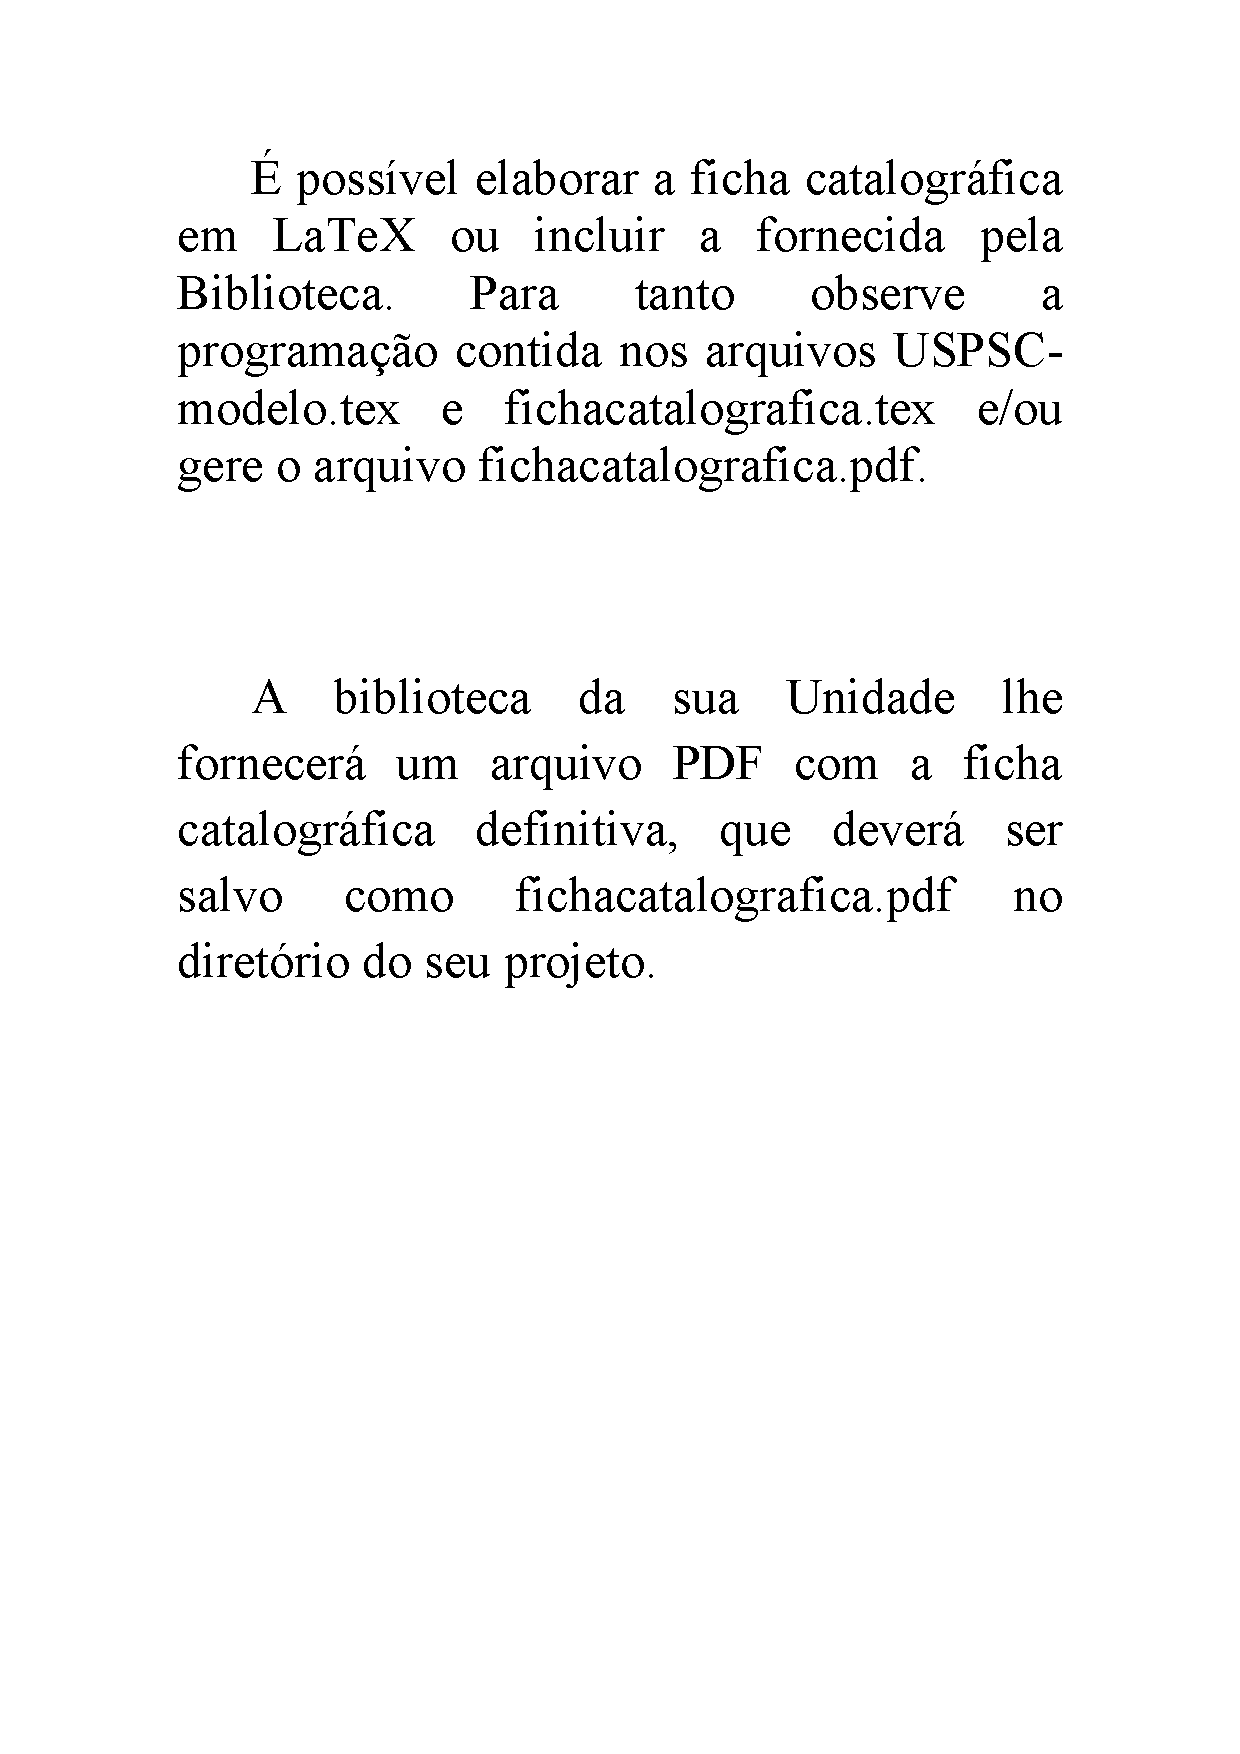
\includepdf{USPSC-TA-PreTextual/USPSC-fichacatalografica.pdf}

% Se voc\^e optar por elaborar a ficha catalogr\'afica, dever\'a 
% incluir uma % antes da linha % antes
% do comando %% USPSC-fichacatalografica.tex
% ---
% Inserir a ficha bibliografica
% ---
% Isto \'e um exemplo de Ficha Catalogr\'afica, ou ``Dados internacionais de
% cataloga\c{c}\~ao-na-publica\c{c}\~ao''. Voc\^e pode utilizar este modelo como refer\^encia. 
% Por\'em, provavelmente a biblioteca da sua universidade lhe fornecer\'a um PDF
% com a ficha catalogr\'afica definitiva ap\'os a defesa do trabalho. Quando estiver
% com o documento, salve-o como PDF no diret\'orio do seu projeto e substitua todo
% o conte\'udo de implementa\c{c}\~ao deste arquivo pelo comando abaixo:
%
\begin{fichacatalografica}
	\hspace{-1.4cm}
	\imprimirnotaautorizacao \\ \\
	%\sffamily
	\vspace*{\fill}					% Posi\c{c}\~ao vertical
\begin{center}					% Minipage Centralizado
  \imprimirnotabib \\
  \begin{table}[htb]
	\scriptsize
	\centering	
	\begin{tabular}{|p{0.9cm} p{8.7cm}|}
		\hline
	      & \\
		  &	  \imprimirautorficha     \\
		
		 \imprimircutter & 
							\hspace{0.4cm}\imprimirtitulo~  / ~\imprimirautor~ ;  ~\imprimirorientadorcorpoficha. -- 	\imprimirlocal, \imprimirdata.   \\
		
		  &  % Para incluir nota referente \`a vers\~ao corrigida no corpo da ficha,
			  % incluir % no in\'{\i}cio da linha acima e tirar a % do in\'{\i}cio da linha abaixo
			  %	\hspace{0.4cm} \imprimirtitulo~  / ~\imprimirautor~ ; ~\imprimirorientadorcorpoficha~- ~\imprimirnotafolharosto. -- \imprimirlocal, \imprimirdata.  \\
		
			\hspace{0.4cm}\pageref{LastPage} p. : il. (algumas color.) ; 30 cm.\\ 
		  & \\
		  & 
		    \hspace{0.4cm}\imprimirnotaficha ~--~ 
						  \imprimirunidademin, 
						  \imprimiruniversidademin, 
		                  \imprimirdata. \\ 
		  & \\                 
		   % Para incluir nota referente \`a vers\~ao corrigida em notas,
		    % incluir uma % no in\'{\i}cio da linha acima e	
		    % tirar a % do in\'{\i}cio da linha abaixo
		    % & \hspace{0.4cm}\imprimirnotafolharosto \\ 
		  & \\ 
		  & \hspace{0.4cm}1. LaTeX. 2. abnTeX. 3. Classe USPSC. 4. Editora\c{c}\~ao de texto. 5. Normaliza\c{c}\~ao da documenta\c{c}\~ao. 6. Tese. 7. Disserta\c{c}\~ao. 8. Documentos (elabora\c{c}\~ao). 9. Documentos eletr\^onicos. I. \imprimirorientadorficha. 
		   II. T\'{\i}tulo. \\
	
		     %Se houver co-orientador, inclua % antes da linha (antes de II. T\'{\i}tulo.) 
		     %          e tire a % antes do comando abaixo 
		     %III. T\'{\i}tulo. \\   
		  \hline
	\end{tabular}
  \end{table}
\end{center}
\end{fichacatalografica}
% ---

 
% e retirar o % do comando abaixo
%%% USPSC-fichacatalografica.tex
% ---
% Inserir a ficha bibliografica
% ---
% Isto \'e um exemplo de Ficha Catalogr\'afica, ou ``Dados internacionais de
% cataloga\c{c}\~ao-na-publica\c{c}\~ao''. Voc\^e pode utilizar este modelo como refer\^encia. 
% Por\'em, provavelmente a biblioteca da sua universidade lhe fornecer\'a um PDF
% com a ficha catalogr\'afica definitiva ap\'os a defesa do trabalho. Quando estiver
% com o documento, salve-o como PDF no diret\'orio do seu projeto e substitua todo
% o conte\'udo de implementa\c{c}\~ao deste arquivo pelo comando abaixo:
%
\begin{fichacatalografica}
	\hspace{-1.4cm}
	\imprimirnotaautorizacao \\ \\
	%\sffamily
	\vspace*{\fill}					% Posi\c{c}\~ao vertical
\begin{center}					% Minipage Centralizado
  \imprimirnotabib \\
  \begin{table}[htb]
	\scriptsize
	\centering	
	\begin{tabular}{|p{0.9cm} p{8.7cm}|}
		\hline
	      & \\
		  &	  \imprimirautorficha     \\
		
		 \imprimircutter & 
							\hspace{0.4cm}\imprimirtitulo~  / ~\imprimirautor~ ;  ~\imprimirorientadorcorpoficha. -- 	\imprimirlocal, \imprimirdata.   \\
		
		  &  % Para incluir nota referente \`a vers\~ao corrigida no corpo da ficha,
			  % incluir % no in\'{\i}cio da linha acima e tirar a % do in\'{\i}cio da linha abaixo
			  %	\hspace{0.4cm} \imprimirtitulo~  / ~\imprimirautor~ ; ~\imprimirorientadorcorpoficha~- ~\imprimirnotafolharosto. -- \imprimirlocal, \imprimirdata.  \\
		
			\hspace{0.4cm}\pageref{LastPage} p. : il. (algumas color.) ; 30 cm.\\ 
		  & \\
		  & 
		    \hspace{0.4cm}\imprimirnotaficha ~--~ 
						  \imprimirunidademin, 
						  \imprimiruniversidademin, 
		                  \imprimirdata. \\ 
		  & \\                 
		   % Para incluir nota referente \`a vers\~ao corrigida em notas,
		    % incluir uma % no in\'{\i}cio da linha acima e	
		    % tirar a % do in\'{\i}cio da linha abaixo
		    % & \hspace{0.4cm}\imprimirnotafolharosto \\ 
		  & \\ 
		  & \hspace{0.4cm}1. LaTeX. 2. abnTeX. 3. Classe USPSC. 4. Editora\c{c}\~ao de texto. 5. Normaliza\c{c}\~ao da documenta\c{c}\~ao. 6. Tese. 7. Disserta\c{c}\~ao. 8. Documentos (elabora\c{c}\~ao). 9. Documentos eletr\^onicos. I. \imprimirorientadorficha. 
		   II. T\'{\i}tulo. \\
	
		     %Se houver co-orientador, inclua % antes da linha (antes de II. T\'{\i}tulo.) 
		     %          e tire a % antes do comando abaixo 
		     %III. T\'{\i}tulo. \\   
		  \hline
	\end{tabular}
  \end{table}
\end{center}
\end{fichacatalografica}
% ---


% As informa\c{c}\~oes que comp\~oem a ficha catalogr\'afica est\~ao 
% definidas no arquivo USPSC-pre-textual-UUUU.tex
% ---

% ---
% Folha de rosto adicional
% Para imprimir a folha de rosto adicional, exigida por algumas Unidades, a exemplo do ICMC,
% retire a % antes do comando abaixo

%\imprimirfolhaderostoadic

% ---
% ---
% Inserir errata
% ---


% ---

% ---
% Inserir folha de aprova\c{c}\~ao
% ---

% A Folha de aprova\c{c}\~ao \'e um elemento obrigat\'orio da NBR 4724/2011 (se\c{c}\~ao 4.2.1.3). 
% Ap\'os a defesa/aprova\c{c}\~ao do trabalho, gere o arquivo folhadeaprovacao.pdf da p\'agina assinada pela banca 
% e iclua o arquivo utilizando o comando abaixo:
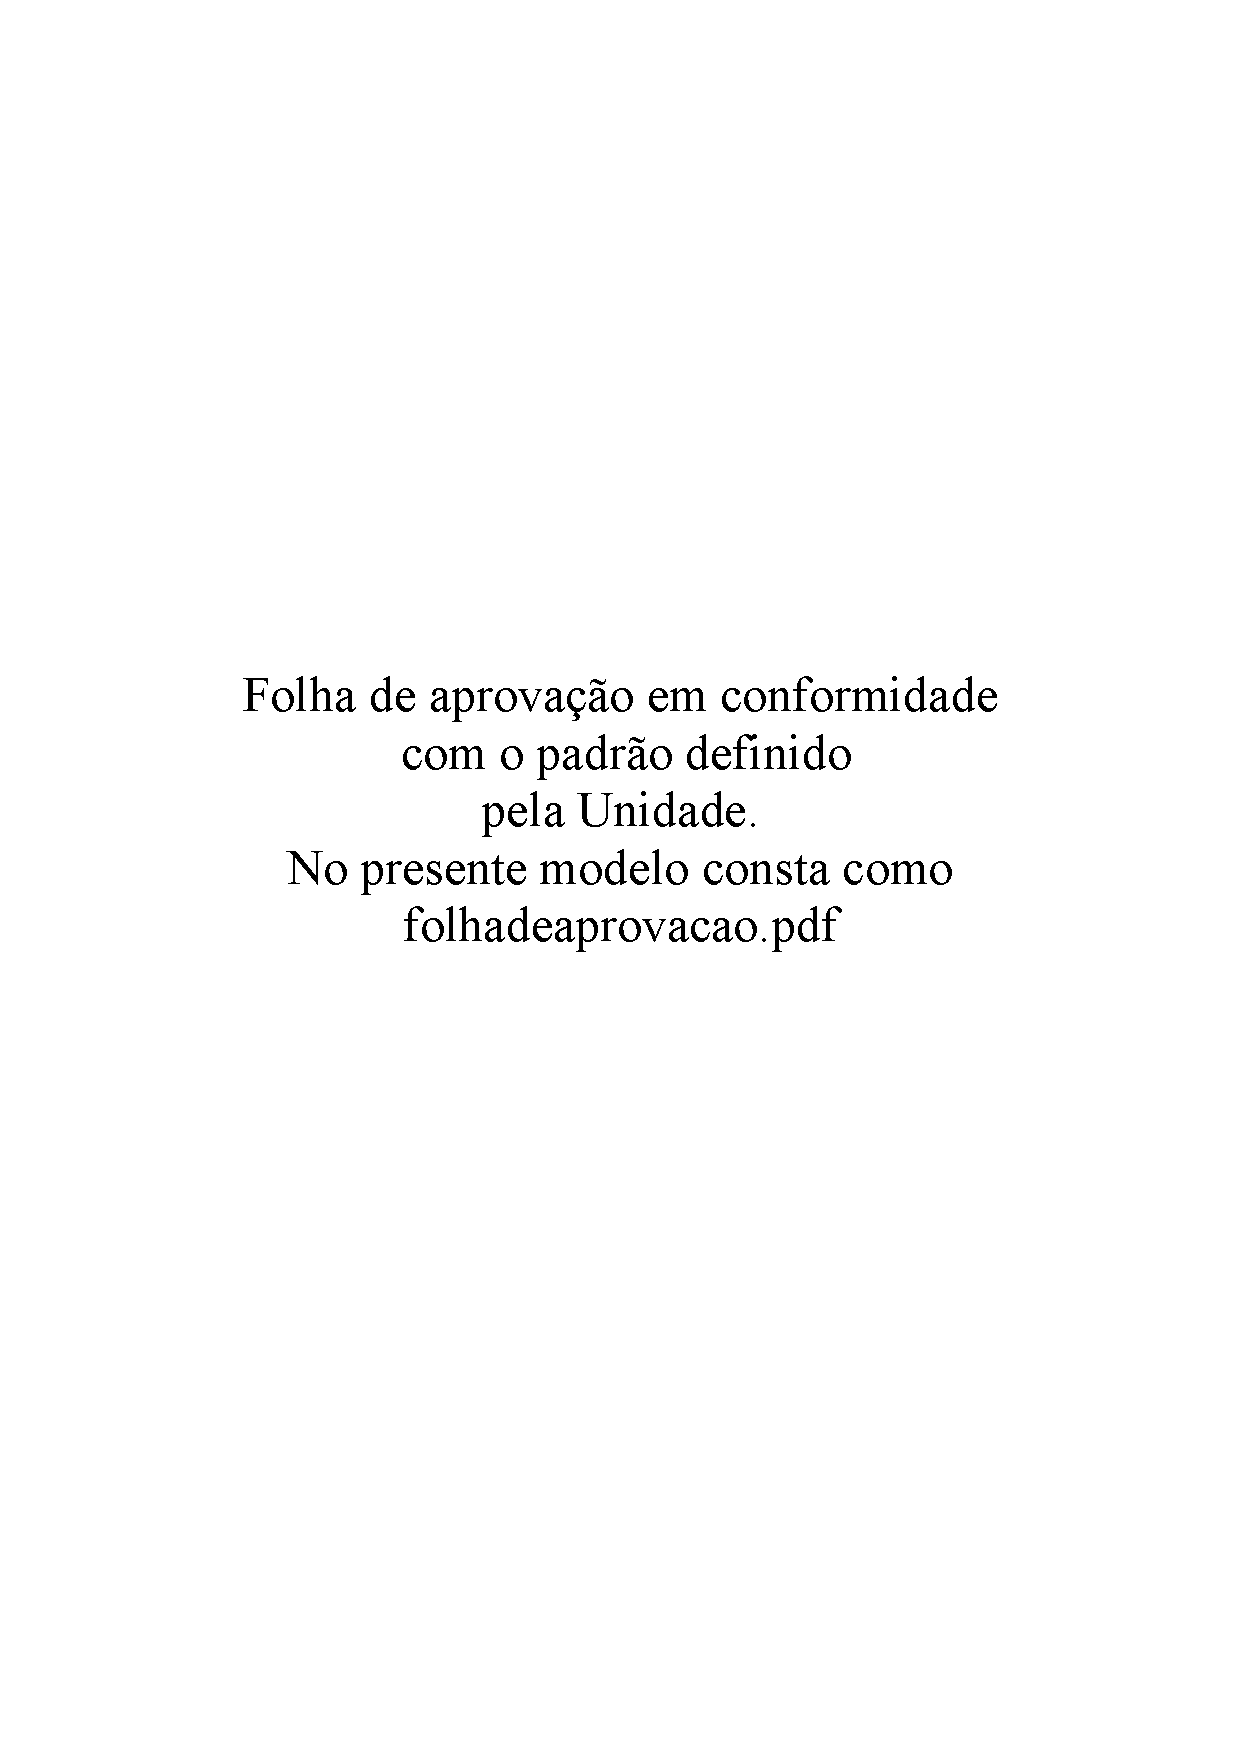
\includepdf{USPSC-TA-PreTextual/USPSC-folhadeaprovacao.pdf}
% Alternativa para a Folha de Aprova\c{c}\~ao:
% Se for a sua op\c{c}\~ao elaborar uma folha de aprova\c{c}\~ao, insira uma % antes do comando acima que inclui o arquivo folhadeaprovacao.pdf,
% tire o % do comando abaixo e altere o arquivo folhadeaprovacao.tex conforme suas necessidades
%\include{folhadeaprovacao}

\includepdf{USPSC-TA-PreTextual/USPSC-PaginaEmBranco.pdf}

% ---
% Dedicat\'oria
% ---
%% USPSC-Dedicatoria.tex
\begin{dedicatoria}
   \vspace*{\fill}
   \centering
   \noindent\textit{@[dedicatoria]@} \vspace*{\fill}
\end{dedicatoria}
% ---
% ---

% ---
% Agradecimentos
% ---
%% USPSC-Agradecimentos.tex
\begin{agradecimentos}
Quero expressar minha gratid\~ao \`as crian\c{c}as e aos jovens; que passaram pelo WASH; que est\~ao conosco e que ser\~ao o futuro do Programa.
Em especial, agrade\c{c}o a uma “crian\c{c}a sempre viva”, ativa, presente, curiosa e que outrora usou o LOGO, gostou de fazer seu jogo e trouxe essa experi\^encia para o seu mundo adulto de cientista, professor, pesquisador, gestor, amigo e companheiro de luta, h\'a mais de uma d\'ecada. Refiro-me ao Dr. Victor Pellegrini Mammana, que ao vivenciar esse prazeroso experimento, quis legar a outras crian\c{c}as o \^extase das descobertas e comprovou que \'e poss\'{\i}vel somar esfor\c{c}os da sociedade civil, das unidades de pesquisa e de educa\c{c}\~ao para contribuir com os processos de aprendizagens em ci\^encia e tecnologia.
Sou, tamb\'em, grata ao meu orientador, Prof. Dr Paulo S\'ergio de Camargo Filho pela companhia e orienta\c{c}\~ao, ao Grupo de Pesquisa STEM Education; e \`a banca de avalia\c{c}\~ao, Prof. Dra. Luciane Capelo e Profº. Dr Eduardo Damasceno.
N\~ao posso deixar de mencionar a generosidade e disposi\c{c}\~ao dos professores Drs. Ala\'{\i}de Pellegrini Mammana e Carlos Mammana, que me forneceram preciosas informa\c{c}\~oes para o trabalho.
Agrade\c{c}o, carinhosamente, \`a Professora Dra. Afira Viana Ripper, por sua contribui\c{c}\~ao para a educa\c{c}\~ao cientifica no ensino fundamental; e por participar do v\'{\i}deo, que resgata essa trajet\'oria e foi parte integrante da minha pesquisa.
Algumas pessoas, tamb\'em, precisam ser destacadas, pois foram imprescind\'{\i}veis para o Programa WASH, desde as suas origens, e marcaram essa hist\'oria (precisei colocar em ordem alfab\'etica): Adriane Pinheiro da Silva, Adriana Tito, Aldo Rabelo, Alex \^Angelo, Alexandre C\^andido Paulo, Alisson Alexandre de Ara\'ujo, Aloizio Mercadante, Am\'elia Naomi, Ant\^onio Carlos dos Santos (o Tot\'o), Ant\^onio Pestana, Alexandre Motta, Ana Paula Rodrigues, Andrea Saraiva, Andrea Dias Victor, Andrea Napolitano, Angel Luis, Antonio Bezerra de Albuquerque, Benedita Aparecida Rodrigues de Freitas, Carlinhos Almeida, C\'assia Oliveira, Cec\'{\i}lia Baranauskas, Celio Turino, Mirza Maria Pellicciotta, Celso Pansera, Celso Pan, Chico Sim\~oes, C\'{\i}ntia Cinquini, Claudio Romanelli, Cleide Santos, Mariana Moura, Clotilde Diogo, Ana Carolina de Deus Soares, Daniel Sp\'ozito, Everbal de Castro, Denise  Vieira Pereira, Dilma Rousseff,  Fabiana Kitagawa, F\'abio Couto, Delma  Medeiros, Fernanda Gon\c{c}alves, Gisele Fink, N\'adia Abiel, Gl\'aucia Veloso, Guida Calixto,  Ingridy Janaina Alves, Haissa Gabriela Silva, Irma Passoni, Isabela Maria Vieira Pereira Rodrigues, Jacqueline Baumgratrz, Jaciara Rodrigues dos Santos, Jandira Maria Rodrigues de Freitas, Jos\'e Leonardo de Oliveira, Juliana Moralles Louvison, Juliana Rabelo, Kevin Martins, Layla Xavier, Leila Bomfim, Let\'{\i}cia Mizael, Lucas Gabriel Batista da Silva, Lucas Titon, Luciano Rudinik, Fernando Accorsi, Magna Gon\c{c}alves, Malu Alencar, Marcela Moreira, Marcelo Aguirre, Maria Fernandes, Michel Morandi Alencar, Nelcina Tropardi. Pedro Tourinho, Paula Ropelo, Paulo B\'ufalo, Priya Patel, Rafael de Deus Soares, Rafael Gomes da Cruz, Rafael Proc\'opio, Renan Inqu\'erito, Renata Xavier, Roberta Santana,  Sandra Lanza, Saulo Monteiro, Sebastian Marques, Tayssa Santana,  S\'ergio Benassi, S\'{\i}lvio Ant\^onio Damasceno, S\'{\i}lvio Aparecido Spinella, TC ( Antonio Carlos), Thatiane Verni Lopes de Ara\'ujo, Toni Klaus, Valdirene Maria dos Santos, Vitor de Oliveira Pochmann, Wagner Rodrigo Silva, Wil Namen, dentre tantos outros.
A todas as gera\c{c}\~oes do WASH: as que passaram, as que compartilham conosco, nesse ano de 2023, os 10 anos do Programa: s\~ao colegas, bolsistas, educandos, educadores, cientistas, coordenadores, orientadores, Conselhos de classes, Sindicatos, gestores, pesquisadores, vereadores, comunidades, os entes federados, que acreditam na ci\^encia e no papel transformador da educa\c{c}\~ao.
Meus agradecimentos, tamb\'em. \`as institui\c{c}\~oes parceiras: Conselho Nacional de Desenvolvimento Cient\'{\i}fico e Tecnol\'ogico - CNPq , Funda\c{c}\~ao Arauc\'aria, WASH Paran\'a, Cia Bola de Meia, Legislativo Federal, por meio dos deputados: Ivan Valente, Alex e Luiza Canziani, Alexandre Padilha, Vicentinho, Carlos Zaratini, Orlando Silva e Alexandre Cury, que foram sens\'{\i}veis e valorizaram a educa\c{c}\~ao cientifica, atrav\'es do Programa WASH. Aos legislativos de Prado Ferreira e Dr. Camargo por fazerem o WASH leis municipais. N\~ao posso deixar de reconhecer a contribui\c{c}\~ao da AkiPosso , com o apoio dos colegas Kevin Martins, Adriana Tito, Priya Patel, Caroline Gardemann, Nelcina Tropardi e Daniela Napolitano. Por fim, agrade\c{c}o a minha fam\'{\i}lia, a minha filha, Agatha Abayomi Silva Sene, aos meus pais, Maria Imaculada de Oliveira e Silva e Joaquim Roberto da Silva, ao meu irm\~ao Eduardo Roberto da Silva in memoriam - presente! e ao Alessandro, que contribu\'{\i}ram para que as condi\c{c}\~oes necess\'arias para o desenvolvimento dessa pesquisa fossem as mais leves para a execu\c{c}\~ao do meu estudo.
Termino enfatizando os papeis especiais do Vereador Paulo Bufalo, que est\'a nesta caminhada conosco desde os prim\'ordios do programa, e da Dra. Andrea Dias Victor, servidora do CNPq que permanece aceitando, com compromisso p\'ublico, excel\^encia administrativa e acad\^emica, a carga de gest\~ao do programa WASH, representada por centenas de bolsistas semestrais.
% @[pontoinsercaoparagrafoagradecimento]@

\end{agradecimentos}
% ---
% ---

% ---
% Ep\'{\i}grafe
% ---
%% USPSC-Epigrafe.tex
\begin{epigrafe}
    \vspace*{\fill}
	\begin{flushright}\textit{. Brasil Meu Brasil ande pra frente. Venha com a gente pra Avenida desfilar . \'E chegada a hora da verdade. N\~ao \'e preciso mais voc\^e se disfar\c{c}ar. Levante os panos, mostra tua cara. E assuma essa cara que voc\^e tem. Brasil Terra dos Ianom\^amis. Essas matas s\~ao de Oxossi. Deixa na terra as riquezas de Oxum. Devolva pro povo o que \'e do povo. Bote os malditos pra fora. E vamos refazer essa na\c{c}\~ao. Pois,o pa\'{i}s que  \'e o olho d’\'agua do mundo n\~ao pode ver sofrer. N\~ao pode ver chorar um povo que trabalha, canta e \'e feliz. Chega de tanta injusti\c{c}a, chega de corrup\c{c}\~ao. Vamos arrumar a casa, vamos dividir o nosso ch\~ao. E chega de sofrer e chega de chorar. Oh p\'atria amada idolatrada. Salve-se Brasil! Antonio Carlos (TC) Santos Silva Alu\'{i}zio Jeremias (Samba Enredo, 1988)}
	\end{flushright}
\end{epigrafe}
% ---
% ---

% A T E N \c{C} \~A O
% Se o idioma do texto for em ingl\^es, o abstract deve preceder o resumo
% resumo em portugu\^es
%
% Resumo
% ---
%% USPSC-Resumo.tex
\setlength{\absparsep}{18pt} % ajusta o espa\c{c}amento dos par\'agrafos do resumo
\begin{resumo}
\begin{flushleft} 
\setlength{\absparsep}{0pt} % ajusta o espa\c{c}amento da refer\^encia
\SingleSpacing 
\imprimirautorabr~~\textbf{\imprimirtituloresumo}.\imprimirdata. \pageref{LastPage}p. 
%Substitua p. por f. quando utilizar oneside em \documentclass
%\pageref{LastPage}f.
\imprimirtipotrabalho~-~\imprimirinstituicao, \imprimirlocal, \imprimirdata. 
 \end{flushleft}
\OnehalfSpacing 
O  Programa Workshop de Aficcionados em Software e Hardware (WASH), de educa\c{c}\~ao em Ci\^encia, Tecnologia, Engenharia, Artes e Matem\'atica (STEAM) \'e executado desde 2013 em dezenas de munic\'{\i}pios brasileiros e com milhares de crian\c{c}as atendidas. Ap\'os anos de pr\'atica, as caracter\'{\i}sticas principais foram agrupadas no Documento de Refer\^encia publicado em 2018, anexado \`a Portaria CTI 178/2018. Esta pesquisa \'e dividida em 2 eixos: m\'etodo historiogr\'afico (eixo 1) e o emprego de consultas estruturadas a uma base de dados especialmente desenvolvida para produzir os indicadores (eixo 2). O trabalho buscou comparar, a partir das defini\c{c}\~oes do Documento de Refer\^encia, \textquotedbl\{\}o que o WASH gostaria de ter sido\textquotedbl\{\} com \textquotedbl\{\}o que o WASH conseguiu ser\textquotedbl\{\}, informa\c{c}\~ao decorrente dos Resultados e An\'alise desta disserta\c{c}\~ao. Para objetivar essa compara\c{c}\~ao, foram formuladas seis hip\'oteses, a partir do Documento de Refer\^encia, que ao final do trabalho foram submetidas a uma valida\c{c}\~ao.  A an\'alise dos sucessos e insucessos dessa valida\c{c}\~ao permitiu produzir uma revis\~ao do Documento de Refer\^encia, a qual \'e o principal produto educacional desta disserta\c{c}\~ao, quesito obrigat\'orio para a obten\c{c}\~ao do t\'{\i}tulo em Mestrado. Agrega-se a esse produto educacional a entrevista com a Profa. Afira Ripper, um dos elementos usados para a an\'alise no eixo 1 e, tamb\'em, um testemunho bastante raro sobre a vinda de Seymour Papert ao Brasil no final do s\'eculo passado.
% @[pontoinsercaoparagraforesumo]@
 

 \textbf{Palavras-chave}: Papert, STEAM, STEM, WASH
\end{resumo}
% ---

% Abstract
% ---
%% USPSC-Abstract.tex
%\autor{Silva, M. J.}
\begin{resumo}[Abstract]
 \begin{otherlanguage*}{english}
	\begin{flushleft} 
		\setlength{\absparsep}{0pt} % ajusta o espaçamento dos par\'agrafos do resumo		
 		\SingleSpacing  		\imprimirautorabr~~\textbf{\imprimirtitleabstract}.	\imprimirdata.  \pageref{LastPage}p. 
		%Substitua p. por f. quando utilizar oneside em \documentclass
		%\pageref{LastPage}f.
		\imprimirtipotrabalhoabs~-~\imprimirinstituicao, \imprimirlocal, 	\imprimirdata. 
 	\end{flushleft}
	\OnehalfSpacing 
   This is the english abstract.

   \vspace{\onelineskip}
 
   \noindent 
   \textbf{Keywords}: LaTeX. USPSC class. Thesis. Dissertation. Conclusion course paper. 
 \end{otherlanguage*}
\end{resumo}

% ---

% ---
% inserir lista de figurass
% ---
\pdfbookmark[0]{\listfigurename}{lof}
\listoffigures*
\cleardoublepage
% ---

% ---
% inserir lista de tabelas
% ---
\pdfbookmark[0]{\listtablename}{lot}
\listoftables*
\cleardoublepage
% ---

% ---
% inserir lista de quadros
% ---
\pdfbookmark[0]{\listofquadroname}{loq}
\listofquadro*
\cleardoublepage
% ---

% ---
% inserir lista de abreviaturas e siglas
% ---
% USPSC-AbreviaturasSiglas.tex
\begin{siglas}
    \item[ABNT] Associação Brasileira de Normas Técnicas
    \item[abnTeX] ABsurdas Normas para TeX
	\item[IBGE] Instituto Brasileiro de Geografia e Estatística
	\item[LaTeX] Lamport TeX
	\item[USP] Universidade de São Paulo
	\item[USPSC] Campus USP de São Carlos
\end{siglas}

% ---

% ---
% inserir lista de s\'{\i}mbolos
% ---
% USPSC-Simbolos.tex
\begin{simbolos}
  \item[$ \Gamma $] Letra grega Gama
  \item[$ \Lambda $] Lambda
  \item[$ \zeta $] Letra grega minúscula zeta
  \item[$ \in $] Pertence
\end{simbolos}
% ---
% ---
% inserir o sumario
% ---
\pdfbookmark[0]{\contentsname}{toc}
\tableofcontents*
\cleardoublepage
% ---
% ----------------------------------------------------------
% ELEMENTOS TEXTUAIS
% ----------------------------------------------------------
\textual
% Os cap\'{\i}tulos s\~ao inseridos como arquivos externos 

% Cap\'{\i}tulo 1 - Introdu\c{c}\~ao
% ---
\chapter[INTRODU\c{C}\~AO]{INTRODU\c{C}\~AO}\label{INTRODU\c{C}\~AO}
Aos olhos de jovens observadores contempor\^aneos, parece natural a relativa desenvoltura com que as pessoas utilizam  as tecnologias da informa\c{c}\~ao e comunica\c{c}\~ao-TIC, em computadores e celulares, nos dias de hoje. J\'a est\~ao bastante difundidos os servi\c{c}os de governo eletr\^onico, os sites de com\'ercio, os  aplicativos de entrega, as plataformas de ensino, de reuni\~oes, a busca por oportunidades profissionais, educacionais, o sistema de urna eletr\^onica, os servi\c{c}os financeiros, como o pix, por exemplo.












Desta forma, \'e poss\'{\i}vel afirmar que as pessoas t\^em usado com frequ\^encia  as ferramentas digitais: aplicativos de mensagens, buscadores (browsers), correio eletr\^onico, redes sociais, entre outras.












Essa no\c{c}\~ao de que os servi\c{c}os digitais no Brasil est\~ao bastante difundidos pode ser confirmada pela grande quantidade de usu\'arios de plataformas como o iFood e o PIX, por exemplo, ou de redes sociais tais como FaceBook, Twitter, Instagram e Google. No caso do iFood, a empresa divulgou que em 2021, por exemplo, seu aplicativo foi \textquotedbl\{\}baixado\textquotedbl\{\} cerca de 1.5 milh\~oes de vezes por m\^es , o que viabilizou a entrega mensal de cerca de 60 milh\~oes de pedidos  (CANALTECH, 2022). A Ag\^encia Brasil, por seu lado, indica que o n\'umero de usu\'arios de PIX chegou a 51 milh\~oes de pessoas em mar\c{c}o de 2022  (M\'aximo, 2022). O n\'umero de trabalhadores em plataformas digitais tamb\'em \'e representativo, chegando a 1.5 milh\~ao de pessoas  (Manzano e Krein, 2022). Nas redes sociais, segundo o site internacional Statista, especializado em indicadores do mundo digital, o Brasil representa o quinto maior mercado, com 165 milh\~oes de usu\'arios, em 2022. Corrobora com essa no\c{c}\~ao de acesso cada vez mais disseminado no Brasil o gr\'afico da Fig. 1, que indica a evolu\c{c}\~ao percentual dos domic\'{\i}lios com acesso \`a internet.














\captionsetup{format=plain}
\begin{figure}[max size={\textwidth}{\textheight}]

\centering


\begin{minipage}[b]{0.4\linewidth}
        \centering
                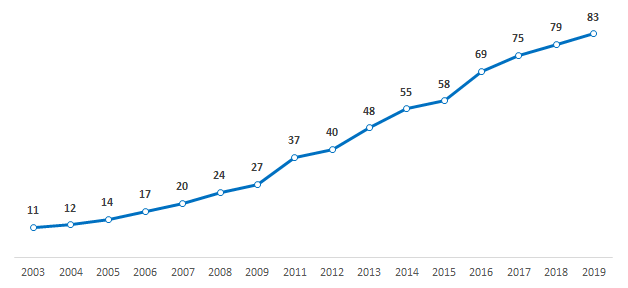
\includegraphics[width=1.0\linewidth]{../../imagens/acesso-internet.png}
                \caption{Evolu\c{c}\~ao do percentual de domic\'{i}lios com acesso para internet (Fonte: SIDRA 2016-2019  (apud [[Schmitz et al., 2021]]))}
                \label{dc69b8cf40fae2ba00158e43d2db2d294110957c}
\end{minipage}%
\hspace{0.5cm}
\end{figure}



As novas gera\c{c}\~oes precisam saber que n\~ao foi sempre assim. Muito embora a percep\c{c}\~ao corrente de que o uso de computadores e celulares \'e indispens\'avel para o conv\'{\i}vio na sociedade, a rigor seu uso \'e relativamente recente.












\'E poss\'{\i}vel identificar a evolu\c{c}\~ao das telecomunica\c{c}\~oes, a partir do s\'eculo passado, como origem das transforma\c{c}\~oes tecnol\'ogicas e digitais disponibilizadas em larga escala. PIERRE LEVY, no livro \textquotedbl\{\}Cibercultura\textquotedbl\{\} (LEVY, 2000):













\noindent\begin{center}\mbox{\centering\fbox{\centering\par\parbox{0.7\linewidth}{\small\textit{\textquotedbl\{\}Durante uma entrevista nos anos 50, Albert Einstein (1879-1955) declarou que tr\^es grandes bombas haviam  explodido durante o s\'eculo XX: a bomba demogr\'afica, a bomba at\^omica e a bomba das telecomunica\c{c}\~oes. Aquilo que Einstein chamou de bomba das telecomunica\c{c}\~oes foi chamado, por meu amigo Roy Ascott (um dos pioneiros e principais te\'oricos da arte em rede), de segundo dil\'uvio, o das informa\c{c}\~oes. As telecomunica\c{c}\~oes geram esse novo dil\'uvio por conta da natureza exponencial, explosiva e ca\'otica de seu crescimento. A quantidade bruta de dados dispon\'{\i}veis se multiplica e se acelera. A densidade dos links entre as informa\c{c}\~oes aumenta vertiginosamente nos bancos de dados, nos hipertextos  e nas redes. Os contatos transversais entre os indiv\'{\i}duos proliferam de forma an\'arquica. \'E o  transbordamento ca\'otico das informa\c{c}\~oes, inunda\c{c}\~ao de dados\textquotedbl\{\}.}\normalsize}}}\end{center}


Ainda, segundo Pierre Levy,













\noindent\begin{center}\mbox{\centering\fbox{\centering\par\parbox{0.7\linewidth}{\small\textit{\textquotedbl\{\}O segundo dil\'uvio n\~ao ter\'a fim. N\~ao h\'a nenhum fundo s\'olido sob o oceano de informa\c{c}\~oes. Devemos aceit\'a-lo como nossa nova condi\c{c}\~ao. Temos que ensinar nossos filhos a nadar, a flutuar, talvez a navegar.\textquotedbl\{\}}\normalsize}}}\end{center}


Para a sociedade chegar nesse ponto, os governos e a iniciativa privada tiveram que, continuamente, investir no desenvolvimento de inova\c{c}\~oes cient\'{\i}ficas e tecnol\'ogicas,  provendo a infraestrutura de comunica\c{c}\~oes e de redes digitais, bem como os meios de acesso a essas redes. O esfor\c{c}o cient\'{\i}fico e tecnol\'ogico de p\'os- guerra americano, liderado por Vannevar Bush a partir do relat\'orio \textquotedbl\{\}Science - The endless frontier\textquotedbl\{\}(5 de julho de 1945), foi o  motivador da cria\c{c}\~ao do National Science Foundation, em 1950; e pode ser considerado  o ponto de partida para o protagonismo do Estado no investimento em inova\c{c}\~oes tecnol\'ogicas, na segunda metade do s\'eculo XX.












Em outra ponta, os governos tiveram que formular pol\'{\i}ticas p\'ublicas para disponibilizar e preparar os cidad\~aos para que pudessem se apropriar dessas tecnologias.












A partir da segunda metade do s\'eculo XX, as redes digitais estavam vinculadas \`a academia, \`as institui\c{c}\~oes de pesquisa e \`a \'area de defesa  (ARPANET, 2022), num contexto de coordena\c{c}\~ao estatal.












No in\'{\i}cio da \'ultima d\'ecada do s\'eculo XX, essas inova\c{c}\~oes  foram avan\c{c}ando em dire\c{c}\~ao ao suprimento das necessidades de relacionamento do cidad\~ao com o governo. Ap\'os esse per\'{\i}odo, os servi\c{c}os baseados nestas inova\c{c}\~oes foram mais longe e alcan\c{c}aram  os demais aspectos dos indiv\'{\i}duos;inclusive na sua rela\c{c}\~ao com os prestadores de servi\c{c}os privados.












Essa expans\~ao ocorreu como resultado de v\'arias a\c{c}\~oes e a sua universaliza\c{c}\~ao \'e consequ\^encia do surgimento de novas formas de relacionamento social, viabilizadas pelas redes digitais, que tornaram mais acess\'{\i}veis novas ferramentas.












Tais transforma\c{c}\~oes tiveram impactos econ\^omicos e sociais profundos, inclusive nas rela\c{c}\~oes de trabalho, tanto na cria\c{c}\~ao e extin\c{c}\~ao de postos de trabalho,quanto em suas formas de contrata\c{c}\~ao, jornada e remunera\c{c}\~ao; acarretando a precariza\c{c}\~ao dos direitos trabalhistas. Essas mudan\c{c}as est\~ao bem descritas  no relat\'orio da Unesco  de 2004 \textquotedbl\{\}Social Transformation in an Information Society: Rethinking Access to You and the World\textquotedbl\{\} (DUTTON, 2004).












A amplitude destas transforma\c{c}\~oes foi sintetizada no conceito de \textquotedbl\{\}Sociedade da Informa\c{c}\~ao\textquotedbl\{\}, \`as vezes, referido como \textquotedbl\{\}Era Digital\textquotedbl\{\} ou \textquotedbl\{\}Era da Informa\c{c}\~ao\textquotedbl\{\}.












O efeito dessas transforma\c{c}\~oes no mundo do trabalho exige dos governos, das empresas e dos cidad\~aos uma constante e r\'apida readapta\c{c}\~ao  nas rela\c{c}\~oes de produ\c{c}\~ao, de novos saberes, e de  compet\^encias. Tamb\'em o sistema educacional vem sendo desafiado a se adaptar, uma vez que \'e dele que se espera o preparo dos cidad\~aos para a nova realidade.












Inicialmente essas mudan\c{c}as eram associadas \`a substitui\c{c}\~ao do trabalho humano decorrente da automa\c{c}\~ao industrial. Mas a radicaliza\c{c}\~ao no uso de solu\c{c}\~oes digitais, inclusive de intelig\^encia artificial, associadas ao aumento da conectividade, v\^em substituindo, segundo  Manyika (2016), \textquotedbl\{\}capacidades cognitivas que antes eram exclusivas de humanos\textquotedbl\{\}. Uma das consequ\^encias mais radicais \'e o surgimento de novos meios de explora\c{c}\~ao humana, representados pela \textquotedbl\{\}Gigs Economy\textquotedbl\{\}  (Manyika, 2016) ou \textquotedbl\{\}Economia do Bico\textquotedbl\{\}, que precariza as rela\c{c}\~oes trabalhistas por meio de plataformas, que as impessoaliza a ponto de camuflar a explora\c{c}\~ao. O termo \textquotedbl\{\}bico\textquotedbl\{\} aqui est\'a sendo usado como tradu\c{c}\~ao livre de \textquotedbl\{\}gigs\textquotedbl\{\}, que nos Estados Unidos \'e uma g\'{\i}ria usada para trabalho tempor\'ario. A uberiza\c{c}\~ao \'e um exemplo de rela\c{c}\~ao de trabalho no contexto da Gigs Economy.












V\'arios pa\'{\i}ses t\^em buscado uma melhor prepara\c{c}\~ao para enfrentar essas transforma\c{c}\~oes. Para isso, t\^em procurado remodelar seus sistemas educacionais, uma vez que um eventual atraso em rela\c{c}\~ao aos demais pa\'{\i}ses pode afetar a prosperidade (CONGRESS, 1998)  de suas popula\c{c}\~oes, sua autonomia e liberdade.












Mais do que \textquotedbl\{\}treinar\textquotedbl\{\} os cidad\~aos, quanto ao uso  de servi\c{c}os digitais, a educa\c{c}\~ao tem um papel fundamental de prepar\'a-los para a sua inser\c{c}\~ao aut\^onoma e digna na sociedade, transformada pelas tecnologias de informa\c{c}\~ao e comunica\c{c}\~ao. Portanto, o desafio do Estado n\~ao se limita a estabelecer pol\'{\i}ticas p\'ublicas de provimento de infraestrutura para que o cidad\~ao possa ter acesso e se beneficiar dos recursos digitais e de comunica\c{c}\~ao, mas, principalmente, preparar estes cidad\~aos para que contribuam com a  constru\c{c}\~ao desses recursos, beneficiando-se da autonomia e prosperidade, que  essa constru\c{c}\~ao gera.












O cidad\~ao, tamb\'em, precisa ser capaz de entender \textquotedbl\{\}o que est\'a por tr\'as\textquotedbl\{\} desses sistemas digitais, para que possa reagir aos excessos da \textquotedbl\{\}algoritimiza\c{c}\~ao\textquotedbl\{\} de suas rela\c{c}\~oes com outros indiv\'{\i}duos.












Assim, antecipando  uma das conclus\~oes desta disserta\c{c}\~ao, \'e no contexto do \textquotedbl\{\}segundo dil\'uvio\textquotedbl\{\} de Ascott que se insere a necessidade de um programa educacional como o WASH.












A percep\c{c}\~ao da import\^ancia da educa\c{c}\~ao para a prosperidade da sociedade n\~ao \'e novidade. No caso americano, por exemplo, remonta aos prim\'ordios de sua independ\^encia. Em termos globais, \'e poss\'{\i}vel perceber o reconhecimento de sua import\^ancia desde a Gr\'ecia e do Egito antigos.












No cap\'{\i}tulo \textquotedbl\{\}Fundamenta\c{c}\~ao Te\'orica,\textquotedbl\{\} revisaremos as origens do conceito de \textquotedbl\{\}Science, Technology, Engineering and Mathematics\textquotedbl\{\} (STEM), mostrando que em, 1.790, o presidente George Washington, em seu primeiro discurso do \textquotedbl\{\}Estado da Uni\~ao\textquotedbl\{\}, enaltecia a ci\^encia e a literatura como  basilares para a \textquotedbl\{\}felicidade p\'ublica\textquotedbl\{\} [(Relat\'orio CRS para o Congresso, www.crs.gov, 2012)]. Essa percep\c{c}\~ao de valor da ci\^encia e da cultura perdura at\'e os dias atuais. Em muitos momentos foi estimulada, inclusive, como resposta \`as amea\c{c}as externas, como foi o caso da mobiliza\c{c}\~ao americana para fazer frente ao sucesso sovi\'etico no programa espacial, representado pelo pioneirismo do lan\c{c}amento do sat\'elite Sputnik, no final da d\'ecada de 50. \'E no cen\'ario da Guerra Fria, que a pol\'{\i}tica de educa\c{c}\~ao em STEM e alfabetiza\c{c}\~ao cient\'{\i}fica e tecnol\'ogica passaram a ser vistas mais claramente como um bem comum, mesmo muito antes do uso desse acr\^onimo de forma oficial.












N\~ao obstante esta permanente percep\c{c}\~ao p\'ublica da import\^ancia e do valor da ci\^encia, os Estados Unidos n\~ao conseguiram manter uma forma\c{c}\~ao de qualidade nas \'areas STEM.












Nos anos 90, os EUA identificaram fragilidades na educa\c{c}\~ao STEM com preju\'{\i}zo ao \textquotedbl\{\}poderio b\'elico e tecnol\'ogico nacional\textquotedbl\{\}, \`a inser\c{c}\~ao de seus cidad\~aos no novo mundo do trabalho, de forma aut\^onoma, soberana  e pr\'ospera. Essas fragilidades foram, relativamente evidenciadas pelo baixo desempenho de adolescentes americanos no \textquotedbl\{\}Programme for International Student Assessment\textquotedbl\{\} (PISA)  (CATTERALL, 2017). Com isso, o governo americano teve que propor a\c{c}\~oes para atualizar as compet\^encias curriculares, visando manter uma inser\c{c}\~ao hegem\^onica na economia do s\'eculo XXI.












Segundo o Relat\'orio \textquotedbl\{\}Congress Research Service\textquotedbl\{\} (CRS - Servi\c{c}o de pesquisa do Congresso Americano), mais de 200 projetos de Lei contendo o termo \textquotedbl\{\}educa\c{c}\~ao cient\'{\i}fica\textquotedbl\{\} foram apresentados entre o per\'{\i}odo de 1987 a 2008. O mesmo relat\'orio aponta que 13 ag\^encias federais estavam envolvidas em programas ou atividades de educa\c{c}\~ao \textquotedbl\{\}STEM\textquotedbl\{\}. (Pag.2 do Relat\'orio)












Os atores governamentais e estudiosos daquele per\'{\i}odo identificaram que faltava aos EUA uma pol\'{\i}tica nacional, uniforme e inclusiva de ensino de ci\^encias, pois era poss\'{\i}vel categorizar diferentes \^enfases sobre o assunto no vasto sistema educacional americano  (CATTERALL, 2017)












Mas, existia tamb\'em, o reconhecido pioneirismo da comunidade acad\^emica americana nos m\'etodos voltados ao aprendizado de temas relacionados ao STEM, ainda que n\~ao identificados sob esse acr\^onimo ou mesmo que n\~ao amplamente disseminados em seu sistema educacional, como viriam a reconhecer os relat\'orios do congresso americano  (CONGRESS, 1998).












Seymour Papert, matem\'atico sul-africano, radicado nos EUA, do Laborat\'orio de Intelig\^encia Artificial do Massachusetts Institute of Technology (MIT), foi um  cientista e educador que acreditava  no  uso do computador como forma de revolucionar o sistema  educacional,  desde os anos 60.












Papert foi um cientista vision\'ario, ao pensar a aprendizagem de crian\c{c}as de forma diferente. Em 1968, escreveu o artigo, \textquotedbl\{\} Teaching Children Thinking \textquotedbl\{\}  em que abordava  o tema sobre crian\c{c}as, educa\c{c}\~ao e computadores. No cap\'{\i}tulo de Fundamenta\c{c}\~ao Te\'orica, sua contribui\c{c}\~ao ser\'a aprofundada, mas \'e necess\'ario antecipar, aqui, alguns elementos para que seja poss\'{\i}vel delimitar o escopo da presente pesquisa.












Cabe reconhecer, de forma resumida, que, quando Papert formulou suas ideias, nos anos 70, os computadores ainda n\~ao eram amplamente acess\'{\i}veis ou dispon\'{\i}veis para uso dom\'estico. Naquele tempo, no existia conceito de \textquotedbl\{\}microcomputadores\textquotedbl\{\}. Equipamentos com poder de processamento milhares de vezes inferior ao de um notebook ocupavam centenas de metros quadrados  (CIPOLI, 2012). Segundo  SOLOMON et al. (2020) , \textquotedbl\{\}em 1.966, os computadores eram poucos, grandes e espalhados\textquotedbl\{\}, os custos eram muito altos e o acesso era muito restrito.












Mas, mesmo na forma de mainframes centralizados (computadores de grande porte) com as limita\c{c}\~oes indicadas acima, foi poss\'{\i}vel a Papert realizar incurs\~oes desbravadoras no campo da aprendizagem para crian\c{c}as utilizando computadores, ainda que sem uma ampla dissemina\c{c}\~ao no sistema educacional americano.












Uma gera\c{c}\~ao de educadores foi formada em torno das ideias de Papert, para quem a pr\'atica de programa\c{c}\~ao de computadores, j\'a no ensino fundamental, poderia ter um papel importante no aprendizado de muitas disciplinas, tais como matem\'atica, ci\^encias e linguagem. A proposta de Papert, at\'e por enfatizar o aprendizado de crian\c{c}as, n\~ao tinha qualquer ambi\c{c}\~ao de capacita\c{c}\~ao profissional e, por si s\'o, n\~ao visava diretamente fazer frente aos desafios do \textquotedbl\{\}mundo do trabalho\textquotedbl\{\}, que foram sendo introduzidos pelas transforma\c{c}\~oes inerentes \`a Sociedade da Informa\c{c}\~ao, nas d\'ecadas subsequentes. Para Papert o uso do computador poderia funcionar como indutor da aprendizagem de um amplo espectro de disciplinas.












Diferentemente de um simples treinamento para usar computadores, o m\'etodo de Papert representava uma mudan\c{c}a em paradigmas educacionais, focalizando a aprendizagem em detrimento do ensino  (NEGROPONTE, 2004). A ideia era \textquotedbl\{\}aprender o que se precisa\textquotedbl\{\} e n\~ao \textquotedbl\{\}aprender o que se deve\textquotedbl\{\}.












O car\'ater estritamente educacional e a peculiar abordagem das propostas de Papert s\~ao apontados em \textquotedbl\{\}Brazil Plan\textquotedbl\{\}  (NEGROPONTE, 2004), embora muito a posteriori por seus colegas, como uma alternativa para a inser\c{c}\~ao do indiv\'{\i}duo na \textquotedbl\{\}era digital\textquotedbl\{\} (digital age).












Assumindo que o conceito de \textquotedbl\{\}era digital \textquotedbl\{\} se refere \`as transforma\c{c}\~oes tecnol\'ogicas que viabilizaram a \textquotedbl\{\}Sociedade da Informa\c{c}\~ao\textquotedbl\{\},  \'e razo\'avel depreender, a partir do que est\'a presente em Brazil Plan  (NEGROPONTE, 2004), que seus sucessores no MIT, de forma independente, entendiam a proposta de Papert como um caminho natural para a melhor inser\c{c}\~ao dos indiv\'{\i}duos na Sociedade da Informa\c{c}\~ao.












O pioneirismo de Papert permite reconhecer nele uma inspira\c{c}\~ao para as demais iniciativas educacionais no estilo STEM, que vieram depois. Essas iniciativas propunham uma educa\c{c}\~ao despojada de formalismos, voltada para a resolu\c{c}\~ao de problemas, ao inv\'es da hist\'orica obsess\~ao por conte\'udos. Esse tipo de abordagem inspirou boa parte dos conceitos subjacentes como \textquotedbl\{\}maker culture\textquotedbl\{\}, entre outros.












As preocupa\c{c}\~oes com o relativo baixo desempenho em STEM, que se aprofundavam nos EUA, nos anos 90, alcan\c{c}aram o resto do mundo. Come\c{c}aram a surgir propostas para tentar promover a qualifica\c{c}\~ao da educa\c{c}\~ao em pa\'{\i}ses em desenvolvimento, por meio do uso intensivo de computadores, nos moldes do que enxergara Papert em seus trabalhos seminais.












Dentre estas propostas, destaca-se o \textquotedbl\{\}One Laptop per Child-OLPC\textquotedbl\{\}, projeto elaborado por pesquisadores do MIT  (NEGROPONTE, 2004), sucessores dos trabalhos de Papert. Uma descri\c{c}\~ao detalhada sobre as caracter\'{\i}sticas e hist\'oria do OLPC pode ser encontrada no cap\'{\i}tulo de Resultados e An\'alises, bem como em outras refer\^encias  (ALVAREZ, 2015); cabendo antecipar que o OLPC foi apresentado ao governo brasileiro, em 2005, durante o F\'orum Econ\^omico em Davos, como solu\c{c}\~ao para os problemas educacionais brasileiros.












Podemos sintetizar que o OLPC envolvia a distribui\c{c}\~ao massiva de laptops (notebooks) para crian\c{c}as e adolescentes dos ensinos fundamental e m\'edio, com vistas a universalizar o acesso \`a internet, no \^ambito da escola p\'ublica brasileira.












Esta universaliza\c{c}\~ao visava oportunizar v\'arias pr\'aticas pedag\'ogicas da Escola P\'ublica, dentre elas a programa\c{c}\~ao de computadores, consequ\^encia direta do pensamento de Papert. Para que pudesse ser implementada nos prazos e formato pretendidos pelo MIT, a proposta do OLPC comprometeria boa parcela do or\c{c}amento do Minist\'erio da Educa\c{c}\~ao na compra de laptops (notebooks). Foi esse comprometimento, e o risco a ele associado, que estimularam o Governo Brasileiro a buscar formas de avaliar sua efetividade. Segundo a avalia\c{c}\~ao do CTI Renato Archer, do Projeto OLPC  (MAMMANA, 2006), solicitada pela Presid\^encia da Rep\'ublica, a proposta do MIT tinha foco na distribui\c{c}\~ao de equipamentos para estudantes, sem uma vis\~ao estruturada de como as pessoas do sistema educacional brasileiro se apropriariam dessa tecnologia.












A avalia\c{c}\~ao do Projeto OLPC proporcionou uma ressignifica\c{c}\~ao para a proposta, permitindo compreender mais profundamente os desafios do uso intensivo de Tecnologia da Informa\c{c}\~ao e Comunica\c{c}\~ao (TIC), no contexto da escola p\'ublica brasileira e, com isso, propor uma alternativa.












O Programa WASH nasceu como uma proposta alternativa ao OLPC (MAMMANA e TOZZI, 2018), com custo inferior, que n\~ao exigia a aquisi\c{c}\~ao de milh\~oes de equipamentos, mas que se inspirava nos mesmos conceitos exitosos de Papert, que fundamentaram a proposta do OLPC.












Cabe uma breve descri\c{c}\~ao nesta introdu\c{c}\~ao sobre o Programa WASH, ressalvando-se que o aprofundamento constar\'a no cap\'{\i}tulo de Resultados e An\'alise. O WASH busca criar espa\c{c}os de intera\c{c}\~ao, na forma de  viv\^encias ou oficinas praticadas no ambiente da escola b\'asica, que visam a promo\c{c}\~ao dos valores do m\'etodo cient\'{\i}fico. A \^enfase s\~ao atividades relacionadas ao STEM e, posteriormente STEAM, que inclui a arte na lista das disciplinas, como tantos outros autores fizeram no in\'{\i}cio do s\'eculo  (CATTERALL, 2017) (MAMMANA e TOZZI, 2018)  (YAKMAN, 2019). Desta forma, um novo acr\^onimo surgiu agregando Science, Technology Engineering, Arts and Mathematics, o STEAM  (YAKMAN, 2019).












Destarte, de forma sint\'etica, pode-se antecipar que o WASH se constitui em atividades em grupo, no \^ambito do STEAM, realizadas no turno e contraturno da escola b\'asica, desvinculadas do curr\'{\i}culo da escola formal, cujos valores principais se alicer\c{c}am no m\'etodo cient\'{\i}fico. O WASH n\~ao \'e um curso, mas se constitui em espa\c{c}os de intera\c{c}\~ao humana para experimenta\c{c}\~ao e conviv\^encia entre indiv\'{\i}duos, no contexto do desenvolvimento de projetos de v\'arios n\'{\i}veis de complexidade.












Pela forma como os pilotos do WASH, em anos iniciais, acabaram sendo implementados no contexto do CTI Renato Archer, houve a consolida\c{c}\~ao da vis\~ao de que institui\c{c}\~oes de Pesquisa poderiam atuar nas  pontes entre centros de excel\^encia, o ensino b\'asico e a comunidade. Em particular, a exist\^encia de um conv\^enio entre o CTI e o Instituto Federal de Educa\c{c}\~ao, Ci\^encia e Tecnologia de S\~ao Paulo (IFSP), campus Campinas, no momento da funda\c{c}\~ao do WASH, em 2013-2014, permitiu experimentar o papel que uma universidade poderia ter no projeto. Esta experi\^encia inicial configurou a conceitua\c{c}\~ao do WASH, que perdura at\'e os tempos atuais- dez anos depois, com intensa participa\c{c}\~ao dos campi do IFSP e do IFPR na amplia\c{c}\~ao regional e estadual.












O Programa WASH tem seu m\'etodo descrito por meio do Documento de Refer\^encia, anexo \`a Portaria CTI 178/2018 (ver Fig. 2), que estabelece uma \textquotedbl\{\}liturgia\textquotedbl\{\}  (CNPq, 2020) para realizar oficinas, bem como os pap\'eis de cada participante e sua forma de opera\c{c}\~ao. Mas, \'e evidente que, por ser longevo, alcan\c{c}ando em 2023 a marca de 10 anos, o WASH passou por muitas transforma\c{c}\~oes em rela\c{c}\~ao \`a proposta inicial, requerendo uma constante caracteriza\c{c}\~ao e revis\~ao, com base em indicadores e an\'alise de seus processos.














\captionsetup{format=plain}
\begin{figure}[htb]

	\begin{center}

		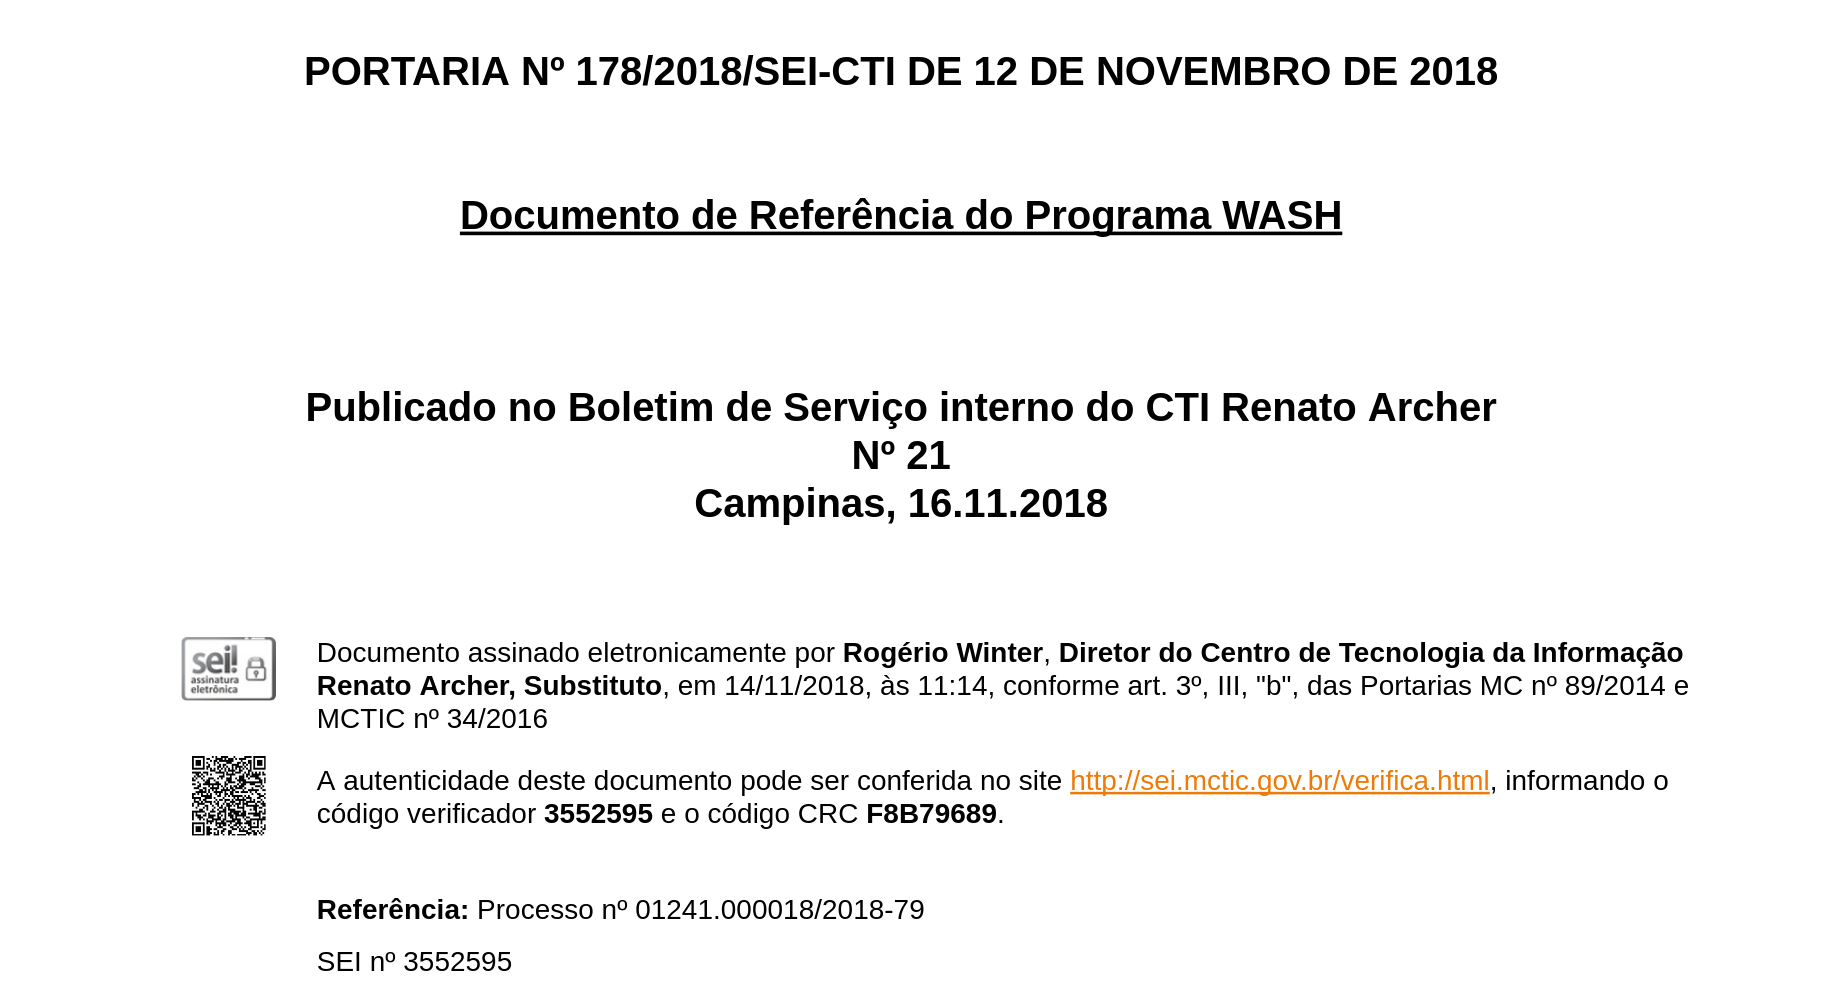
\includegraphics[max size={\textwidth}{\textheight}]{../../imagens/capa-portaria-178.png}

	\end{center}

	\caption{\label{5369350fe31df6a16c506eebf158a3d2b77020ea}Portaria CTI 178-2018, cujo anexo \'e o  Documento de Refer\^encia do Programa WASH. (fonte: SEI-MCTI)}

\end{figure}

Por curioso, n\~ao obstante os criadores do WASH tenham se inspirado nos conceitos pedag\'ogicos do OLPC, tamb\'em opuseram-se \`a aquisi\c{c}\~ao dos notebooks  (MAMMANA e TOZZI, 2018) pelo governo brasileiro, em raz\~ao de outros aspectos do projeto que se mostravam invi\'aveis, nos campos or\c{c}ament\'ario, industrial, ergon\^omico, inclusivo e de log\'{\i}stica  (MAMMANA, 2005a).












Neste trabalho, ser\~ao abordadas a hist\'oria e a caracteriza\c{c}\~ao do Programa WASH. O documento fundamental a ser usado para permitir a caracteriza\c{c}\~ao do WASH \'e a pr\'opria Portaria CTI 178, cujo anexo \'e o documento de refer\^encia do WASH, al\'em de outros registros, tais como publica\c{c}\~oes, relat\'orios, planos de trabalho e produ\c{c}\~ao audiovisual. A an\'alise do documento do WASH permitir\'a compreender \textquotedbl\{\}o que o WASH gostaria de ter sido\textquotedbl\{\}, ao passo que todo o resto do desenvolvimento do trabalho buscar\'a estabeler \textquotedbl\{\}o que o WASH de fato conseguiu ser\textquotedbl\{\}. A partir desses dois entendimentos, ser\'a proposta uma  revis\~ao do Documento de Refer\^encia, com vistas a aprimor\'a-lo.












A abordagem adotada na presente disserta\c{c}\~ao se encaixa no m\'etodo de \textquotedbl\{\}Estudo de Caso\textquotedbl\{\}  e buscar\'a contar, por meio da aplica\c{c}\~ao de um m\'etodo historiogr\'afico, toda essa trajet\'oria que se inicia no que foi descrito aqui, bem como identificar o m\'etodo do Programa WASH e seus resultados.












\section[WASH: projeto, programa, sistema, organiza\c{c}\~ao ou pol\'{\i}tica p\'ublica?]{WASH: projeto, programa, sistema, organiza\c{c}\~ao ou pol\'{\i}tica p\'ublica?}\label{WASH: projeto, programa, sistema, organiza\c{c}\~ao ou pol\'{\i}tica p\'ublica?}
\'E oportuno que se busque, logo no in\'{\i}cio desse estudo, uma uniformiza\c{c}\~ao na denomina\c{c}\~ao do WASH. Trata-se de um projeto, de um programa, de um sistema, de uma organiza\c{c}\~ao ou de uma pol\'{\i}tica p\'ublica?












Para responder a essa pergunta \'e preciso, adiantar que o WASH ocorre no \^ambito de projetos de inicia\c{c}\~ao cient\'{\i}fica e de extens\~ao junto ao Conselho Nacional de Desenvolvimento Cient\'{\i}fico e Tecnol\'ogico-CNPq, financiados por emendas parlamentares, (ver  lista de emendas na se\c{c}\~ao 4.2.1).












Por essa raz\~ao, historicamente, temos nos referido ao WASH como projeto, mas, talvez, n\~ao seja a melhor forma de denomin\'a-lo.












Os planos de trabalho do WASH s\~ao registrados no CNPq e especificam como ser\'a a execu\c{c}\~ao das emendas parlamentares. Os quais est\~ao organizados da seguinte forma:













\begin{alineas}
\item t\'{\i}tulo do projeto;
\item introdu\c{c}\~ao, materiais e m\'etodos;
\item objeto, objetivo e p\'ublico alvo;
\item prazo de execu\c{c}\~ao e entreg\'aveis;
\item identifica\c{c}\~ao da equipe;
\item cronograma e
\item or\c{c}amento.
\end{alineas}

Os planos de trabalho podem ser complementados por aditivos, prorroga\c{c}\~ao de prazo e vig\^encia; mas, em geral, essas altera\c{c}\~oes n\~ao podem ampliar seus escopos de execu\c{c}\~ao.












Iniciado, em 2013, sem financiamento, o WASH recebeu, de 2016 at\'e o 2022, quinze emendas parlamentares, cada uma com seu plano de trabalho espec\'{\i}fico, submetido ao CNPq e registrado na Plataforma Carlos Chagas (CHAGAS (2022)).












Esses planos de trabalho, embora com caracter\'{\i}sticas e escopos espec\'{\i}ficos, seguiram diretrizes de execu\c{c}\~ao que t\^em em comum a promo\c{c}\~ao da aprendizagem STEAM.












Portanto, essa repeti\c{c}\~ao de projetos sequenciais, cada um com sua especifidade, mas todos seguindo a mesma diretriz, indica que o WASH tem caracter\'{\i}sticas de Programa, como \'e poss\'{\i}vel verificar nos conceitos do Project Management Institute  (PMI, 2008), citadas por  Weaver (2010):













\noindent\begin{center}\mbox{\centering\fbox{\centering\par\parbox{0.7\linewidth}{\small\textit{Programas focalizam a coordena\c{c}\~ao de um conjunto de projetos relacionados, bem como de outras atividades, ao longo do tempo, para entregar benef\'{\i}cios para a organiza\c{c}\~ao (Tradu\c{c}\~ao livre de apud. PMI, 2008).}\normalsize}}}\end{center}


Desta forma, \'e razo\'avel aceitar que aquilo que vem sendo chamado de Projeto WASH j\'a possa ser considerado como Programa, dado que \'e justamente um conjunto de Projetos, com atividades coordenadas e com m\'etodos que, emboram evoluam no tempo, seguem uma diretriz.












N\~ao obstante ser poss\'{\i}vel atribuir tacitamente ao WASH uma caracter\'{\i}stica de programa, em termos dos citados conceitos do Project Management Institute (PMI), h\'a mais elementos para se considerar.












A vincula\c{c}\~ao do WASH ao governo federal exige a observ\^ancia de normas para a cria\c{c}\~ao de programas, a exemplo da edi\c{c}\~ao de atos de of\'{\i}cio (portarias, decretos etc) espec\'{\i}ficos para tal.












A aus\^encia desses instrumentos legais, que estabeleceriam um \textquotedbl\{\}programa federal\textquotedbl\{\}, indica que a sobreviv\^encia do WASH depende da aprova\c{c}\~ao, a cada nova emenda parlamentar, das propostas de plano de trabalho apresentadas ao CNPq. Em outras palavras, a exist\^encia do WASH depende da dilig\^encia da equipe na busca constante por recursos financeiros (emendas), bem como da avalia\c{c}\~ao anual, por parte do CNPq e parlamentares, dos resultados alcan\c{c}ados, n\~ao havendo a garantia de continuidade que um programa proveria.












Essa caracter\'{\i}stica exige um cuidado com o uso da palavra \textquotedbl\{\}programa\textquotedbl\{\}, sendo necess\'ario esclarecer o contexto em que pode ser usada, como segue: o WASH efetivamente praticado extrapola os limites de qualquer um dos planos de trabalho, que o implementaram desde sua cria\c{c}\~ao at\'e os dias de hoje.












Por outro lado, veremos, ao longo desta disserta\c{c}\~ao, que tamb\'em \'e poss\'{\i}vel entender o WASH como um sistema, sob a \'otica de uma da defini\c{c}\~ao a seguir:













\noindent\begin{center}\mbox{\centering\fbox{\centering\par\parbox{0.7\linewidth}{\small\textit{\textquotedbl\{\}(Sistema \'e um) conjunto de elementos, concretos ou abstratos, intelectualmente organizados.\textquotedbl\{\} (fonte: Oxford Languages atrav\'es do Google)}\normalsize}}}\end{center}


A defini\c{c}\~ao de sistema trazida por BERTALANFFY (1968) tamb\'em, corrobora com esse entendimento:













\noindent\begin{center}\mbox{\centering\fbox{\centering\par\parbox{0.7\linewidth}{\small\textit{\textquotedbl\{\}Sistema \'e um complexo de elementos interagentes que \'e aberto para o ambiente e interage com ele\textquotedbl\{\} (Fonte:  BERTALANFFY (1968), tradu\c{c}\~ao livre)}\normalsize}}}\end{center}


A import\^ancia de considerar o WASH como um sistema tem a ver com aplica\c{c}\~ao de m\'etodos de an\'alise de sistemas, a exemplo da modelagem de dados relacional para a cria\c{c}\~ao de sua plataforma de gest\~ao, a \textquotedbl\{\}Platu\'oxe\textquotedbl\{\}.












Quanto a verificar se o WASH \'e uma organiza\c{c}\~ao, podemos usar a seguinte defini\c{c}\~ao  (MAXIMIANO, 1981):













\noindent\begin{center}\mbox{\centering\fbox{\centering\par\parbox{0.7\linewidth}{\small\textit{\textquotedbl\{\}As organiza\c{c}\~oes s\~ao grupos sociais deliberadamente orientados para a realiza\c{c}\~ao de objetivos ou finalidades (...)\textquotedbl\{\} (Fonte:  MAXIMIANO (1981))}\normalsize}}}\end{center}


Usando palavras diferentes, o mesmo autor nos contempla com outra forma de defini\c{c}\~ao que \'e particularmente interessante para o WASH:













\noindent\begin{center}\mbox{\centering\fbox{\centering\par\parbox{0.7\linewidth}{\small\textit{(...) uma organiza\c{c}\~ao \'e uma combina\c{c}\~ao de esfor\c{c}os individuais que tem por finalidade realizar prop\'ositos coletivos. Por meio da organiza\c{c}\~ao torna-se poss\'{\i}vel perseguir e alcan\c{c}ar objetivos que seriam inating\'{\i}veis para uma pessoa.\textquotedbl\{\} (Fonte:  MAXIMIANO (1981))}\normalsize}}}\end{center}


As defini\c{c}\~oes de Maximiano indicam a possibilidade de qualificar o WASH tamb\'em, como organiza\c{c}\~ao, dado que ele \'e constitu\'{\i}do por um grupo de pessoas que conjuminam esfor\c{c}os individuais para alcan\c{c}ar prop\'ositos coletivos. Essa possibilidade d\'a a abertura para empregar, em nosso estudo, o m\'etodo historiogr\'afico aplicado \`a administra\c{c}\~ao p\'ublica, como se ver\'a em Materiais e M\'etodos.












O WASH tamb\'em pode ser considerado uma protopol\'{\i}tica p\'ublica, daquelas que s\~ao vivenciadas mas que ainda n\~ao est\~ao formalizadas numa lei federal. Essa possibilidade de entendimento surge de v\'arios elementos, entre eles, a exist\^encia de leis municipais que criaram o WASH nas cidades de Prado Ferreira e Dr. Camargo, ambas no Paran\'a; ou de normas infralegais para a mesma finalidade nas cidades de Jacare\'{\i} (SP)e Santo In\'acio (PR), entre outras. Essas experi\^encias locais servem de piloto para uma poss\'{\i}vel legisla\c{c}\~ao federal, que venha a transformar o WASH em uma pol\'{\i}tica p\'ublica de fato.












Considerando essas delimita\c{c}\~oes conceituais, decidimos adotar, na maior parte das vezes, o ep\'{\i}teto \textquotedbl\{\}Programa\textquotedbl\{\} para qualificar o WASH, sem preju\'{\i}zo para as demais dimens\~oes (sistema, organiza\c{c}\~ao e protopol\'{\i}tica p\'ublica).












Assim, reconhecemos antecipadamente que o WASH tem, as dimens\~oes de programa, sistema, organiza\c{c}\~ao e protopol\'{\i}tica, o que ser\'a demonstrado ao longo do estudo.












\section[Objeto]{Objeto}\label{Objeto}
Este trabalho tem por objeto de estudo a hist\'oria e a caracteriza\c{c}\~ao, do Programa WASH considerando o per\'{\i}odo de novembro de 2013 a outubro de 2022.












\section[Objetivos]{Objetivos}\label{Objetivos}
Essa disserta\c{c}\~ao tem objetivos  \textquotedbl\{\}Gerais\textquotedbl\{\} e \textquotedbl\{\}Espec\'{\i}ficos\textquotedbl\{\}.












\subsection[Objetivo Geral]{Objetivo Geral}\label{Objetivo Geral}
Estudar e caracterizar o Programa WASH em dois eixos:(1)sua hist\'oria e (2) seus indicadores.












\subsection[Objetivos Espec\'{\i}ficos]{Objetivos Espec\'{\i}ficos}\label{Objetivos Espec\'{\i}ficos}














\begin{alineas}
\item identificar no Documento de Refer\^encia (Portaria CTI 178/2018) os pontos que requerem adequa\c{c}\~ao \`as cont\'{\i}nuas mudan\c{c}as sociais e educacionais do pa\'{\i}s, que ocorreram depois da sua edi\c{c}\~ao;
\item verificar se os objetivos presentes nesse documento se concretizaram, atrav\'es da valida\c{c}\~ao das hip\'oteses levantadas nesta disserta\c{c}\~ao;
\item identificar as pr\'aticas do WASH que precisam ser melhoradas;
\item identificar novos conceitos e pr\'aticas que precisam ser incorporados ao WASH; e
\item produzir uma revis\~ao do Documento de Refer\^encia do WASH como produto educacional a ser apresentado ao final desta pesquisa
\end{alineas}

\section[Hip\'oteses]{Hip\'oteses}\label{Hip\'oteses}
Decidimos utilizar como origem das hip\'oteses deste estudo parte dos objetivos presentes na Portaria 178/2018. Assim, podemos dizer que, ao validar uma hip\'otese com essa origem, estamos verificando se aquele objetivo foi alcan\c{c}ado pelo Programa WASH.












Complementarmente aos objetivos da Portaria CTI 178/2018, enunciamos hip\'oteses adicionai, com base em nossa viv\^encia como part\'{\i}cipes do Programa. As hip\'oteses obtidas, a partir dessas duas origens, foram organizadas em uma lista mostrada adiante.












O trabalho de verifica\c{c}\~ao das hip\'oteses \'e imprescind\'{\i}vel para conhecer a efici\^encia e efic\'acia do WASH,como programa de educa\c{c}\~ao.












O fato de um objetivo estar declarado no Documento de Refer\^encia da Portaria CTI 178/2018 n\~ao significa que o mesmo foi alcan\c{c}ado. Neste sentido, esses objetivos, base das hip\'oteses, refletem \textquotedbl\{\}o que o WASH gostaria de ter sido\textquotedbl\{\}. Ao passo que, nesta disserta\c{c}\~ao, verificaremos hip\'otese a hip\'otese, \textquotedbl\{\}o que o WASH conseguiu ser\textquotedbl\{\}. As falhas eventualmente encontradas contribuir\~ao para apontar o caminho que deve ser seguido na revis\~ao do Documento de Refer\^encia.












\subsection[Hip\'otese 1: Efici\^encia e Efic\'acia do WASH]{Hip\'otese 1: Efici\^encia e Efic\'acia do WASH}\label{Hip\'otese 1: Efici\^encia e Efic\'acia do WASH}
O enunciado \'e:













\noindent\begin{center}\mbox{\centering\fbox{\centering\par\parbox{0.7\linewidth}{\small\textit{Hip\'otese 1: O WASH conseguiu promover a dissemina\c{c}\~ao de conhecimentos em Ci\^encia e Tecnologia, beneficiando milhares de pessoas em dezenas de cidades pela oferta de oficinas de curta dura\c{c}\~ao nos ensinos fundamental, m\'edio e superior.}\normalsize}}}\end{center}


O enunciado acima pode ser verificado pela avalia\c{c}\~ao da efici\^encia e efic\'acia do WASH, no contexto do eixo 2-indicadores.












\subsection[Hip\'otese 2: Orienta\c{c}\~ao a Projetos]{Hip\'otese 2: Orienta\c{c}\~ao a Projetos}\label{Hip\'otese 2: Orienta\c{c}\~ao a Projetos}
O enunciado \'e:













\noindent\begin{center}\mbox{\centering\fbox{\centering\par\parbox{0.7\linewidth}{\small\textit{Hip\'otese 2: O WASH estimula a aprendizagem por meio da orienta\c{c}\~ao a projetos para alunos dos ensinos m\'edio e t\'ecnico e gradua\c{c}\~ao em temas relacionados ao STEAM.}\normalsize}}}\end{center}


\subsection[Hip\'otese 3: Origem do WASH]{Hip\'otese 3: Origem do WASH}\label{Hip\'otese 3: Origem do WASH}
O enunciado \'e:













\noindent\begin{center}\mbox{\centering\fbox{\centering\par\parbox{0.7\linewidth}{\small\textit{Hip\'otese 3: O WASH teve como origem: (i)  o aprendizado com a avalia\c{c}\~ao do OLPC (NEGROPONTE, 2004) pelo governo brasileiro; (ii) as pr\'aticas do Programa Governo Eletr\^onico de Servi\c{c}o de Atendimento ao Cidad\~ao (GESAC); e (iii) a Avalia\c{c}\~ao do Programa de Inclus\~ao Digital (PID) da Secretaria de Inclus\~ao Social (SECIS), do Minist\'erio da Ci\^encia e Tecnologia (CGEE, 2009).}\normalsize}}}\end{center}


\subsection[Hip\'otese 4: Pr\'atica Pedag\'ogica do WASH]{Hip\'otese 4: Pr\'atica Pedag\'ogica do WASH}\label{Hip\'otese 4: Pr\'atica Pedag\'ogica do WASH}
O enunciado \'e:













\noindent\begin{center}\mbox{\centering\fbox{\centering\par\parbox{0.7\linewidth}{\small\textit{Hip\'otese 4: O WASH se inspira em conceitos e pr\'aticas de Seymour Papert (PAPERT, 1980), combinados com outros m\'etodos, tendo se embasado, em parte, nas experi\^encias pioneiras da Profa. Dra. Afira Vianna Ripper, na transposi\c{c}\~ao dos conceitos de Papert para o Brasil e no trabalho de inicia\c{c}\~ao cient\'{\i}fica para o ensino fundamental.}\normalsize}}}\end{center}


\subsection[Hip\'otese 5:WASH como proto-pol\'{\i}tica p\'ublica]{Hip\'otese 5:WASH como proto-pol\'{\i}tica p\'ublica}\label{Hip\'otese 5:WASH como proto-pol\'{\i}tica p\'ublica}
O enunciado \'e:













\noindent\begin{center}\mbox{\centering\fbox{\centering\par\parbox{0.7\linewidth}{\small\textit{Hip\'otese 5: O WASH pode ser considerado como uma protopol\'{\i}tica p\'ublica nacional, apesar da Portaria CTI 178/2018 n\~ao se constituir em um instrumento de cria\c{c}\~ao desse tipo de pol\'{\i}tica.}\normalsize}}}\end{center}


\subsection[Hip\'otese 6: WASH como organiza\c{c}\~ao heter\'arquica]{Hip\'otese 6: WASH como organiza\c{c}\~ao heter\'arquica}\label{Hip\'otese 6: WASH como organiza\c{c}\~ao heter\'arquica}
O enunciado \'e:













\noindent\begin{center}\mbox{\centering\fbox{\centering\par\parbox{0.7\linewidth}{\small\textit{Hip\'otese 6: Em termos organizacionais, o WASH \'e estruturado atrav\'es de rela\c{c}\~oes heter\'arquicas.}\normalsize}}}\end{center}


\section[Problema]{Problema}\label{Problema}
Com a passagem dos anos,os desafios do Programa WASH foram se transformando. Pr\'aticas tiveram que ser adaptadas e outras incorporadas.












Um exemplo eloquente de transforma\c{c}\~ao de realidade, que requeriu revis\~ao de pr\'aticas do WASH, decorreu da pandemia de COVID-19, que exigiu o isolamento social, inviabilizando viv\^encias presenciais.












O Programa WASH que se restringia a atividades presenciais, precisou criar formas de praticar oficinas remotamente, o que contrariava as diretrizes originais que estabeleciam  realiza\c{c}\~ao exclusivamente presencial. Assim, como em todo o resto do sistema escolar, essa imposi\c{c}\~ao exigiu vencer barreiras t\'ecnicas de conectividade e conceituais com rela\c{c}\~ao \`as atividades remotas. Esta transforma\c{c}\~ao de pr\'atica ainda n\~ao est\'a refletida nas diretrizes presentes na Portaria CTI 178/2018.












Outros desafios contempor\^aneos podem ser citados, como a promulga\c{c}\~ao da Lei Geral de Prote\c{c}\~ao de Dados (LGPD), a incorpora\c{c}\~ao do registro de nome social, as transforma\c{c}\~oes tecnol\'ogicas nas ferramentas de programa\c{c}\~ao pedag\'ogica, entre outros. O Documento de Refer\^encia anexado \`a Portaria CTI 178/2018 ,tamb\'em, n\~ao trata esses aspectos.












A verifica\c{c}\~ao ou n\~ao das hip\'oteses elencadas na se\c{c}\~ao anterior, poder\'a contribuir para a identifica\c{c}\~ao de outros problemas.












Isto posto, podemos sintetizar a situa\c{c}\~ao-problema, atrav\'es da seguinte pergunta: \textquotedbl\{\}Quais altera\c{c}\~oes devem ser realizadas no Documento de Refer\^encia do WASH para que o Programa possa evoluir e se adaptar \`as novas realidades?\textquotedbl\{\}












\section[Justificativa]{Justificativa}\label{Justificativa}
A aceita\c{c}\~ao do m\'etodo do Programa WASH pelas institui\c{c}\~oes parceiras espalhadas pelos estados de S\~ao Paulo e Paran\'a, documentada por dezenas de instrumentos legais de ades\~ao (portarias, boletins, entre outros - ver se\c{c}\~ao 4.2.2), permite vislumbrar a transforma\c{c}\~ao do WASH em pol\'{\i}tica p\'ublica. Acreditamos que h\'a um potencial de crescimento nas ades\~oes ao Programa, como resultado de uma almejada melhoria em suas pr\'aticas.












Portanto um pr\'oximo passo, necess\'ario para que o Programa atinja o est\'agio de pol\'{\i}tica p\'ublica consolidada (mas n\~ao suficiente) \'e realizar uma revis\~ao em seu Documento de Refer\^encia, contido no anexo \`a Portaria CTI 178/2018, para que os problemas identificados na se\c{c}\~ao anterior, entre outros, possam ser equacionados.












Alcan\c{c}ado esse objetivo de revis\~ao, outros passos de car\'ater de governo, que fogem ao escopo desse trabalho, ser\~ao necess\'arios.












\chapter[FUNDAMENTA\c{C}\~AO TE\'ORICA ]{FUNDAMENTA\c{C}\~AO TE\'ORICA }\label{FUNDAMENTA\c{C}\~AO TE\'ORICA }
Neste cap\'{\i}tulo, buscaremos a fundamenta\c{c}\~ao para a vindoura escolha dos m\'etodos, que ser\~ao efetivamente empregados para alcan\c{c}ar os objetivos deste estudo.












Assim, o presente cap\'{\i}tulo, tamb\'em, \'e dividido nos dois eixos principais da presente investiga\c{c}\~ao:













\begin{alineas}
\item Eixo 1: hist\'oria
\item Eixo 2: indicadores
\end{alineas}

Antes de prosseguir \'e necess\'ario entender o papel do m\'etodo em um trabalho cient\'{\i}fico. Essa compreens\~ao pode ser constru\'{\i}da pela an\'alise da origem etmol\'ogica da palavra.













\noindent\begin{center}\mbox{\centering\fbox{\centering\par\parbox{0.7\linewidth}{\small\textit{\textquotedbl\{\}O \'etimo latino “methodus” \'e um dos fundamentos para a significa\c{c}\~ao do termo “m\'etodo”. Com o sentido de caminho (“chemin”, “route”), do grego odos (Cl\'edat, 1914, 213), est\'a presente em v\'arios idiomas: “methode” (Al), “m\'ethode” (Fr), “m\'etodo” (Esp), “metodo” (It). Com o methodus e o seu significado mais abrangente, “caminho” (way, Weg, route, via e camino), designamos o nosso tipo ideal.\textquotedbl\{\} (fonte: (FREITAS, 2019) )}\normalsize}}}\end{center}


Tendo em vista a necessidade de escolher um caminho para chegar  aos objetivos desta pesquisa, ser\~ao descritos os fundamentos te\'oricos, que ser\~ao considerados para essa escolha de m\'etodo.












Portanto, neste cap\'{\i}tulo, n\~ao trataremos dos m\'etodos efetivamente utilizados no trabalho, mas das op\c{c}\~oes que consideramos para escolher os m\'etodos que de fato utilizamos.












\'E preciso declarar que temos sensibilidade aos argumentos apresentados por GODOI et al. (2006), dando conta da impossibilidade \textquotedbl\{\} do m\'etodo como corretor ou rem\'edio, para as dificuldades \textquotedbl\{\} inerentes a uma inevit\'avel inseguran\c{c}a epistemol\'ogica\textquotedbl\{\}. Entretanto, n\~ao haver\'a como nos debru\c{c}armos sobre isso com mais profundidade, havendo que prosseguir, mesmo que t\~ao somente para, em car\'ater preliminar, \textquotedbl\{\}adquirir conhecimento de maneira instrumental\textquotedbl\{\}, de uma busca por uma sempre question\'avel \textquotedbl\{\}objetividade cient\'{\i}fica\textquotedbl\{\} (GODOI et al., 2006), com a esperan\c{c}a de plantar uma semente para que outras abordagens possam se somar a nossa, contribuindo para a constru\c{c}\~ao do conhecimento.












Uma caracter\'{\i}stica da pesquisa bibliogr\'afica, que apresentamos aqui, \'e seu  car\'ater instrumental, n\~ao voltado para gerar novos conhecimentos (interpreta\c{c}\~oes) sobre a literatura em si.












Nosso objetivo principal \'e o de melhorar o Documento de Refer\^encia do Programa WASH e, para isso, decidimos otimizar nosso trabalho, usufruindo da colabora\c{c}\~ao de outros pesquisadores que j\'a se debru\c{c}aram sobre os cl\'assicos e  sintetizaram os m\'etodos de nosso interesse.












Assim, nossa escolha bibliogr\'afica sintetiza e consolida conhecimentos complementares que est\~ao nos cl\'assicos. Mas, fazemos isso sempre de forma cr\'{\i}tica, para n\~ao nos apoiarmos em textos de baixa confiabilidade.












Essa forma dita \textquotedbl\{\} pragm\'atica \textquotedbl\{\} de abordagem nos permite avan\c{c}ar no que realmente temos para contribuir, nos apoiando com seguran\c{c}a no trabalho de compila\c{c}\~ao e interpreta\c{c}\~ao que outros j\'a fizeram nas diversas \'areas onde temos interesse. Al\'em disso, nossa abordagem instrumental exige a explora\c{c}\~ao de refer\^encias mais recentes, porque essas acabam por compilar conhecimentos de v\'arias \'areas, apresentando descri\c{c}\~oes de m\'etodos encapsuladas em formatos prontamente aplic\'aveis.












Finalmente, faz parte dessa fundamenta\c{c}\~ao te\'orica uma revis\~ao de alguns conceitos gerais, que permear\~ao todo o texto, os quais est\~ao presentes na \'ultima se\c{c}\~ao deste cap\'{\i}tulo.












\section[Fundamenta\c{c}\~ao: hist\'oria (eixo 1)]{Fundamenta\c{c}\~ao: hist\'oria (eixo 1)}\label{Fundamenta\c{c}\~ao: hist\'oria (eixo 1)}
Para  tra\c{c}ar a hist\'oria e caracterizar o Programa WASH, o contexto no qual ele surgiu, quais pol\'{\i}ticas, projetos e  a\c{c}\~oes, enfim, as diversas experi\^encias que o antecederam (ver Hip\'oteses), faz-se  necess\'ario que seja definido e aplicado o m\'etodo. Mas, antes de defini-lo, revisitaremos conceitos pr\'e-existentes que  desenvolveremos nesta se\c{c}\~ao.












Assim, nesta se\c{c}\~ao, complementada pelo Ap\^endice A, ser\'a revisitada a base te\'orica das pr\'aticas historiogr\'aficas, dispon\'{\i}veis para construir as narrativas sobre atividades e conceitos, que antecederam a exist\^encia do Programa WASH, a exemplo do GESAC, do OLPC e do Pensamento de Papert.

























Ocorre que, pelo car\'ater recente de muitas das hist\'orias que contribu\'{\i}ram para exist\^encia do WASH, elas ainda est\~ao sendo contadas por diversos perspectivas e atores. Por ter sido testemunha ocular de algumas delas, esta autora tem a contribuir com sua pr\'opria narrativa, a qual n\~ao pode ficar restrita a uma simples cr\^onica ou descri\c{c}\~ao de linha do tempo. Ao contr\'ario, o eixo 1 foi desenvolvido de forma complementar ao eixo 2, estabelecendo uma abordagem plural, que deve culminar com a proposta de mudan\c{c}as no Documento de Refer\^encia do WASH.












A nossa reconhecida proximidade com os fatos, que tentamos descrever e narrar nesta disserta\c{c}\~ao, exige um cuidado especial, porque, como alerta  PIERANTI (2022):













\noindent\begin{center}\mbox{\centering\fbox{\centering\par\parbox{0.7\linewidth}{\small\textit{\textquotedbl\{\}(...) a perspectiva do autor est\'a intrinsicamente ligada ao seu modo de ver e expor a Hist\'oria, sendo determinante, em parte, do seu relato e das interpreta\c{c}\~oes da\'{\i} decorrentes. (...)\textquotedbl\{\} (fonte:  (PIERANTI, 2022)}\normalsize}}}\end{center}


Esse risco n\~ao \'e novidade e pode-se dizer que foi abordado por Pierre Nora  (apud DOSSE (2012)), criador da ego-hist\'oria, nos anos 80, quando o historiador assumia publicamente sua subjetividade. Considerando que, neste trabalho, estamos fazendo um tipo de \textquotedbl\{\}hist\'oria do tempo presente\textquotedbl\{\}  (DOSSE, 2012), pelo car\'ater recente do per\'{\i}odo abordado, \'e indispens\'avel \textquotedbl\{\}conhecer o lugar de enuncia\c{c}\~ao do historiador, a institui\c{c}\~ao necess\'aria em fun\c{c}\~ao da qual ele conduz sua investiga\c{c}\~ao e o momento preciso durante o qual ele escreve a sua pr\'atica \textquotedbl\{\}  (DOSSE, 2012).












Esse reconhecimento de que se trata de uma hist\'oria de tempo presente permite, de uma forma alternativa, considerar nosso trabalho, tamb\'em, como um estudo de uma organiza\c{c}\~ao, onde o WASH assume essa dimens\~ao, sem desconsiderar seu car\'ater de  programa, sistema ou protopol\'{\i}tica.












Assim sendo, n\~ao seria surpresa se algu\'em propusesse o emprego de m\'etodos de administra\c{c}\~ao, pertinentes \`a disciplina de \textquotedbl\{\}Organiza\c{c}\~ao, Sistemas de M\'etodos\textquotedbl\{\} (OSM) para estudar o WASH.













\noindent\begin{center}\mbox{\centering\fbox{\centering\par\parbox{0.7\linewidth}{\small\textit{Organiza\c{c}\~ao, Sistemas e M\'etodos \'e uma \'area da administra\c{c}\~ao, que lida com um conjunto de t\'ecnicas, que t\^em como objetivo principal aperfei\c{c}oar o funcionamento das organiza\c{c}\~oes. (Fonte: CARDOSO (2014) )}\normalsize}}}\end{center}


O WASH n\~ao pode ser considerado uma institui\c{c}\~ao dentro do Servi\c{c}o P\'ublico Federal, porque carece de equipe est\'avel ou documento formal de institucionaliza\c{c}\~ao, que defina um organograma ou outra forma de hierarquia, t\~ao cara \`as corpora\c{c}\~oes. Dentro da classifica\c{c}\~ao de organiza\c{c}\~oes oferecida por MAXIMIANO (1981), o WASH n\~ao se encaixa integralmente em \textquotedbl\{\}Grupos Sociais Secund\'arios\textquotedbl\{\}, que \'e justamente o grupo que tem caracter\'{\i}sticas de institucionaliza\c{c}\~ao adequadas para o emprego da OSM.












Por esse motivo, concentraremos nosso trabalho nos dois eixos j\'a elencados, sem o emprego da OSM.












Um outro aspecto a ser considerado \'e a posi\c{c}\~ao da presente autora, que \'e part\'{\i}cipe do Programa/Organiza\c{c}\~ao, representado pelo WASH. A literatura nos socorre com a vis\~ao de que \'e imposs\'{\i}vel \textquotedbl\{\}negar a natureza humana do pesquisador e (...) seu conjunto de refer\^encias comuns ao tempo presente\textquotedbl\{\} (PIERANTI, 2022), mesmo quando o pesquisador est\'a \textquotedbl\{\}distante da \'epoca e do local estudados\textquotedbl\{\}. Refor\c{c}a a confian\c{c}a na possibilidade da autora produzir uma contribui\c{c}\~ao relevante para o  estudo, mesmo com um envolvimento pr\'oximo  \`a compreens\~ao de que \textquotedbl\{\}deve prevalecer o reconhecimento das limita\c{c}\~oes da historiografia, implicando na aceita\c{c}\~ao dos resultados obtidos como um encaminhamento, dentre outros poss\'{\i}veis da pesquisa proposta\textquotedbl\{\} (PIERANTI, 2022).












 FAVERSANI (1998) corrobora com esse entendimento, quando traz:













\noindent\begin{center}\mbox{\centering\fbox{\centering\par\parbox{0.7\linewidth}{\small\textit{O discurso cient\'{\i}fico, assim, n\~ao exige que se elimine a subjetividade do pesquisador, mas imp\~oe que esta seja expl\'{\i}cita em seus tra\c{c}os fundamentais, pressupondo que o cientista tenha que ter, necessariamente, clareza de quais as convic\c{c}\~oes que o movem quando realiza o seu trabalho, de quais id\'eias ele traz subjacentes quando exerce seu of\'{\i}cio que tem por fun\c{c}\~ao, entre outras coisas, criar elementos para a forma\c{c}\~ao de opini\~oes em sua sociedade. (Fonte:  FAVERSANI (1998))}\normalsize}}}\end{center}


Tamb\'em, conforta-nos a vis\~ao da epistemologia social que aponta para dois aspectos complementares, in verbis  (GODOI et al., 2006) : \textquotedbl\{\}a quest\~ao da impossibilidade do distanciamento e da assepsia metodol\'ogica ao lan\c{c}armos olhares sobre o mundo; e o fato de que somos necessariamente parte daquilo que analisamos e, muitas vezes, tentamos modificar\textquotedbl\{\}.












Ademais, desafia a nossa ambi\c{c}\~ao de \textquotedbl\{\}encontrar um m\'etodo\textquotedbl\{\} \`a compreens\~ao de que a \textquotedbl\{\}historiografia n\~ao produziu um \'unico m\'etodo, mas diferentes tradi\c{c}\~oes\textquotedbl\{\}  (Firat, 1987).  Esse desafio se aprofunda, quando consideramos, por exemplo, Costa e Silva (2019), que apontam que a \textquotedbl\{\}pesquisa hist\'orica ainda pode ser considerada marginal na maioria dos livros sobre metodologia de pesquisa em ci\^encias sociais, pois n\~ao desfruta do espa\c{c}o dado a outros m\'etodos de pesquisa\textquotedbl\{\}, in verbis. Lan\c{c}ando nossa ambi\c{c}\~ao num limbo,  Costa e Silva (2019) reconhecem \textquotedbl\{\}que um dos argumentos mais fortes acerca dessa aus\^encia (de descri\c{c}\~ao de m\'etodo) transfere uma certa responsabilidade para o historiador, que n\~ao teria, por pr\'atica de pesquisa, de justificar metodologicamente o seu trabalho\textquotedbl\{\}.












Para al\'em de nos desafiar, muitas vezes, sent\'{\i}mo-nos arrefecidos em nosso intento de \textquotedbl\{\}encontrar um m\'etodo\textquotedbl\{\} para o registro hist\'orico, tendo em vista a nega\c{c}\~ao de Popper em rela\c{c}\~ao \`a cientificidade da hist\'oria antiga, por exemplo (FAVERSANI, 1998), ou mesmo de sua utilidade (Firat, 1987).












Os historiadores v\^em dando respostas a estes questionamentos, como no caso do exemplo citado por  Costa e Silva (2019), que relata a publica\c{c}\~ao, em 2013, pela revista \textquotedbl\{\}Management and Organizational History\textquotedbl\{\} (\textquotedbl\{\}Gest\~ao e Hist\'oria Organizacional\textquotedbl\{\}, em tradu\c{c}\~ao livre), de uma edi\c{c}\~ao especial entitulada \textquotedbl\{\}Doing Research in Management and Organizational Studies\textquotedbl\{\} (\textquotedbl\{\}Fazendo pesquisa em gest\~ao e em estudos organizacionais\textquotedbl\{\}, em tradu\c{c}\~ao livre). Esta edi\c{c}\~ao especial \'e voltada para apresentar aplica\c{c}\~oes do m\'etodo hist\'orico, com orienta\c{c}\~oes pr\'aticas  (Costa e Silva, 2019) para o mundo dos estudos organizacionais. A mesma refer\^encia traz outros exemplos de iniciativas recentes semelhantes.












Dessa forma, n\~ao podemos nos deixar abater por essas quest\~oes epistemol\'ogicas, pelo menos do ponto de vista do trabalho historiogr\'afico, que precisa ser realizado nesta disserta\c{c}\~ao, cabendo adotar uma vis\~ao pragm\'atica para a quest\~ao, inspirada pelo entendimento de FAVERSANI (1998):













\noindent\begin{center}\mbox{\centering\fbox{\centering\par\parbox{0.7\linewidth}{\small\textit{Se assumimos uma postura cient\'{\i}fica, temos que o trabalho resultante sempre apresentar\'a a seu leitor quais os caminhos que foram trilhados para obter determinados resultados, quais as  fontes foram utilizadas para se realizar este trabalho e quais os conceitos que servem de par\^ametro para a leitura de fontes. Este rigor n\~ao \'e um mero capricho, mas uma rotina necess\'aria para que este trabalho possa ser \'util a outros pesquisadores, que se dedicam a pesquisas semelhantes, \`a medida que estes poder\~ao, com estes elementos em m\~aos, extrair muito maior proveito para suas pr\'oprias reflex\~oes. (Fonte:  FAVERSANI (1998))}\normalsize}}}\end{center}


As busca pela verifica\c{c}\~ao das Hip\'oteses indica uma complexidade que exige uma vis\~ao sist\^emica entre abordagens hist\'oricas (eixo 1) e levamentamento estat\'{\i}stico de dados para a produ\c{c}\~ao de indicadores (eixo 2). Esta men\c{c}\~ao a uma pluralidade de m\'etodos e, em particular, a men\c{c}\~ao ao uso da estat\'{\i}stica, nos motiva a olhar com mais cuidado para a segunda fase da Escola de Annales, quando se praticou a \textquotedbl\{\}Hist\'oria Quantitativa\textquotedbl\{\} (ver Ap\^endice A). Fazemos isso com o devido cuidado de n\~ao suscitar expectativas nos leitores que, depois, n\~ao conseguiremos satisfazer. Esse olhar, para a segunda fase da Escola de Annales, como refer\^encia para o nosso trabalho, ser\'a feito com a devida parcim\^onia e consci\^encia do papel, limitado que podemos desempenhar em termos de historiografia.












Esta necessidade de uma vis\~ao sist\^emica, que respeita os contextos presentes, \'e sustentada por v\'arios autores e bem sintetizada em uma frase de PIERANTI (2022):













\noindent\begin{center}\mbox{\centering\fbox{\centering\par\parbox{0.7\linewidth}{\small\textit{\textquotedbl\{\}An\'alises descontextualizadas perdem sua relev\^ancia, na medida em que se tornam pouco fact\'{\i}veis ou possivelmente deslocadas da realidade\textquotedbl\{\} (PIERANTI, 2022)}\normalsize}}}\end{center}


Com isso em mente, no cap\'{\i}tulo de Materias e M\'etodos, tentaremos estabelecer um caminho pr\'oprio de historiografia, com inspira\c{c}\~ao na possibilidade de aplicar o m\'etodo historiogr\'afico como elemento de pesquisa em administra\c{c}\~ao p\'ublica contempor\^anea, seguindo as op\c{c}\~oes indicadas em   Costa e Silva (2019) e PIERANTI (2022), por exemplo. Esta iniciativa parte da aceita\c{c}\~ao da hist\'oria, como determinante para explicar os acontecimentos e estruturas existentes em qualquer sociedade (PIERANTI, 2022) e, consequentemente, em suas organiza\c{c}\~oes. Mas, tal aceita\c{c}\~ao n\~ao esteve sempre presente na disciplina de Estudos Organizacionais, a exemplo da \textquotedbl\{\}forte influ\^encia cientificista norte-americana, que resultou em um afastamento da hist\'oria, conferindo um car\'ater a-hist\'orico \`as pesquisas\textquotedbl\{\}  (Costa e Silva, 2019).












Kieser (1994)  analisa o motivo pelo qual a hist\'oria teria sido \textquotedbl\{\}expelida\textquotedbl\{\} de pr\'aticas recentes da Teoria das Organiza\c{c}\~oes. Citando Max Weber como um dos pais dessa \'area, bem como da sociologia, Kieser indica que Weber estaria \textquotedbl\{\}convencido que para entender institui\c{c}\~oes contempor\^aneas seria necess\'ario conhecer como elas se desenvolveram na hist\'oria\textquotedbl\{\}  (Kieser, 1994, tradu\c{c}\~ao livre). Segundo ele, uma das raz\~oes para essa neglig\^encia com a hist\'oria, contrariando a prescri\c{c}\~ao de Weber, seria a recente profissionaliza\c{c}\~ao da sociologia, que na busca de uma identidade que a tornasse independente, desenvolveu a prefer\^encia por m\'etodos espec\'{\i}ficos tais como experimentos e entrevistas, que \textquotedbl\{\}em conjun\c{c}\~ao com a an\'alise estat\'{\i}stica, ofereciam um prospecto de metodologia precisa, an\'aloga \`a da ci\^encia\textquotedbl\{\}  (Kieser, 1994, tradu\c{c}\~ao livre).












Tendo em mente que caracterizar o WASH \'e uma forma de estudo organizacional, nos parece adequado dedicar uma parcela do esfor\c{c}o deste trabalho \`a hist\'oria, ainda que seja necess\'ario manter nossa ambi\c{c}\~ao auto-limitada, porque tratamos de eventos muito recentes, sem um compromisso com a hist\'oria de longa dura\c{c}\~ao, como \'e o caso da contribui\c{c}\~ao dos grandes nomes da Escola de Annales, por exemplo.












Mesmo com a consci\^encia desse limite, entendemos que \'e poss\'{\i}vel contribuir com os registros que ser\~ao trazidos no cap\'{\i}tulo de resultados, desta disserta\c{c}\~ao, para que outros pesquisadores possam se debru\c{c}ar com mais profundidade sobre os eventos que descrevemos e narramos em car\'ater pioneiro.












\subsection[Revis\~ao: historiografia]{Revis\~ao: historiografia}\label{Revis\~ao: historiografia}
Para que nosso trabalho vinculado ao eixo 1 n\~ao ficasse sem uma identidade dentro do universo das tradi\c{c}\~oes historiogr\'aficas, decidimos fazer uma revis\~ao das principais escolas.












Por outro lado, tal revis\~ao, ainda que muito resumida, mostrou-se por demais extensa para os objetivos deste trabalho, raz\~ao pela qual est\'a sendo apresentada no Ap\^endice A, desta disserta\c{c}\~ao.












A revis\~ao apresentada permite avaliar em que medida o m\'etodo historiogr\'afico escolhido e descrito em Materiais e M\'etodos carrega elementos da \textquotedbl\{\}Hist\'oria Quantitativa\textquotedbl\{\} da segunda fase da Escola de Annales.












\subsection[Hierarquia versus heterarquia]{Hierarquia versus heterarquia}\label{Hierarquia versus heterarquia}
A literatura traz muitas formas de definir heterarquia e, frequentemente, se vale de exemplos e situa\c{c}\~oes hist\'oricas para isso. Trata-se de um termo  recente introduzido  por  McCULLOCH (1945), em seu estudo sobre a organiza\c{c}\~ao dos neur\^onios no c\'erebro humano  (CRUMLEY, 1995). Esse trabalho foi disruptivo para a \'area de neuroci\^encias, porque demonstrou que n\~ao existe hierarquia entre neur\^onios no c\'erebro humano  (CRUMLEY, 1995).












A partir de  McCULLOCH (1945), o termo se espalhou para outras \'areas de, a exemplo das ci\^encias sociais, redes de computadores e teoria das organiza\c{c}\~oes  (PERLO et al., 2012). O emprego do termo em cada \'area espec\'{\i}fica tem nuances pr\'oprias.












Como o conceito de heterarquia \'e colocado em oposi\c{c}\~ao ao de hierarquia, vamos iniciar nossa discuss\~ao com a defini\c{c}\~ao de hierarquia (CRUMLEY, 1995):













\noindent\begin{center}\mbox{\centering\fbox{\centering\par\parbox{0.7\linewidth}{\small\textit{\textquotedbl\{\}(...) elementos que na base de certos fatores est\~ao subordinados a outros e podem ser ordenados (ranked)\textquotedbl\{\} (Fonte:  CRUMLEY (1995), tradu\c{c}\~ao livre)}\normalsize}}}\end{center}


Heterarquia \'e definida, por  CRUMLEY (1995), como:













\noindent\begin{center}\mbox{\centering\fbox{\centering\par\parbox{0.7\linewidth}{\small\textit{\textquotedbl\{\}(...) rela\c{c}\~ao entre elementos em que eles n\~ao est\~ao ordenados (ranked) ou quando eles t\^em o potencial de serem ordenados (ranked) em diferentes formas.\textquotedbl\{\}}\normalsize}}}\end{center}


A literatura cita (PERLO et al., 2012) e (DA SILVA, 2017), a exemplifica\c{c}\~ao de um sistema heter\'arquico, a partir da experi\^encia da Batalha de Midway, (1942) no Pac\'{\i}fico, quando a frota americana derrotou a japonesa.












Nesse epis\'odio, os americanos perderam sua nau capit\^ania (USS Yorktown) em pouco tempo de combate, obrigando uma reorganiza\c{c}\~ao do comando. Segundo Von Foerster (apud  PERLO et al. (2012)), como resposta a esta situa\c{c}\~ao, houve um movimento espont\^aneo dos v\'arios comandantes de navios americanos para que assumissem \'a frente das iniciativas b\'elicas, em fun\c{c}\~ao da percep\c{c}\~ao que tinham da posi\c{c}\~ao privilegiada de observa\c{c}\~ao do teatro naval, em cada momento. Como resultado dessa iniciativa de \textquotedbl\{\}quebrar a hierarquia\textquotedbl\{\}, os americanos conseguiram vencer a batalha.












Esse exemplo \'e curioso, porque as for\c{c}as armadas s\~ao reconhecidamente como hier\'ariquicas, mas a batalha de Midway mostra uma situa\c{c}\~ao em que essa organiza\c{c}\~ao teve que ser substitu\'{\i}da, mesmo que temporariamente, por uma heterarquia.












N\~ao poder\'{\i}amos nos furtar de citar a defini\c{c}\~ao de heterarquia presente na Wikipedia, porque a pr\'opria forma de organiza\c{c}\~ao e produ\c{c}\~ao de conte\'udos daquela enciclop\'edia \'e considerada como um exemplo de heter\'arquia  (CASTILHO, 2008).












Segundo a Wikipedia, no verbete \textquotedbl\{\}heterarquia\textquotedbl\{\} consta que:













\noindent\begin{center}\mbox{\centering\fbox{\centering\par\parbox{0.7\linewidth}{\small\textit{\textquotedbl\{\}Heterarquia (...), sistema onde n\~ao h\'a um controle centralizado vertical, mas predomina uma ordem consensual. \'E diferente da homoarquia, aus\^encia de centraliza\c{c}\~ao e coer\c{c}\~ao; e da hierarquia, ordem centralizada e verticalizada.\textquotedbl\{\} (Fonte: Wikipedia)}\normalsize}}}\end{center}


 CASTILHO (2008) define a heterarquia como segue:













\noindent\begin{center}\mbox{\centering\fbox{\centering\par\parbox{0.7\linewidth}{\small\textit{\textquotedbl\{\}(a heterarquia) procura definir uma forma de trabalho coletivo onde n\~ao h\'a um superior e nem uma agenda ou m\'etodo imposto de cima para baixo, por meio de chefias hierarquizadas. No sistema heter\'arquico existe uma ordem, decidida pela maioria, ao contr\'ario da anarquia, onde n\~ao existe ordem alguma.\textquotedbl\{\} (Fonte:  CASTILHO (2008))}\normalsize}}}\end{center}


Neste trabalho,s\~ao importantes os questionamentos trazidos por Papert se a hierarquia seria um modo adequado de organiza\c{c}\~ao para a educa\c{c}\~ao  (PAPERT, 1994). Segundo Papert:













\noindent\begin{center}\mbox{\centering\fbox{\centering\par\parbox{0.7\linewidth}{\small\textit{\textquotedbl\{\}H\'a atividades em que a organiza\c{c}\~ao hier\'arquica \'e obrigat\'oria: o ex\'ercito \'e um exemplo \'obvio. Num outro extremo, h\'a atividades em que qualquer pessoa sensata consideraria a organiza\c{c}\~ao hier\'arquica como absurda - por exemplo, em poesia ou pintura. Em outras \'areas, h\'a espa\c{c}o para a escolha no equil\'{\i}brio entre hierarquia e seu oposto - para o qual sigo Warren McCulloch ao usar o nome heterarquia, que sugere um sistema no qual cada elemento \'e igualmente governado por todos os outros.\textquotedbl\{\} (fonte:  PAPERT (1994))}\normalsize}}}\end{center}


\subsection[Governo Eletr\^onico]{Governo Eletr\^onico}\label{Governo Eletr\^onico}
Foi no s\'eculo XIX, que os primeiros conceitos de programa\c{c}\~ao come\c{c}aram a ser desenvolvidos. O mec\^anico franc\^es, Joseph-Marie Jacquard, (1752-1854) inventou o primeiro tear automatizado, utilizando a inova\c{c}\~ao dos cart\~oes perfurados. Outros contribuintes foram Charles Baggage (1791-1871) e Ada Lovelace (1815-1852), com o desenvolvimento do conceito de m\'aquina anal\'{\i}tica, embora a m\'aquina, propriamente dita, n\~ao tenha sido efetivamente constru\'{\i}da. No entanto, mesmo assim, seus esfor\c{c}os s\~ao considerados basilares para o desenvolvimento dos primeiros computadores. Ada Lovelace foi considerada a primeira pessoa efetivamente a se valer do conceito de programa\c{c}\~ao na Hist\'oria.












O empres\'ario norte americano, Herman Hollerith, (1860-1929) desenvolveu um sistema capaz de computar dados. Seu desenvolvimento se deu no contexto de uma demanda de Governo. Desde 1880, o governo americano fazia o censo demogr\'afico e demorava 8 anos para contabilizar os dados. Hollerith criou uma m\'aquina capaz de computar as informa\c{c}\~oes coletadas, durante o censo de 1890, tamb\'em, a partir de cart\~oes perfurados, diminuindo assim o tempo de c\'alculo para apenas dois anos e meio. Esse exemplo talvez seja uma das primeiras formas de emprego de uma tecnologia digital primitiva numa atividade de governo. Mas n\~ao era uma tecnologia voltada para disponibilizar servi\c{c}os diretamente para o cidad\~ao, um conceito que veio a se concretizar muitas d\'ecadas depois.












A partir desta iniciativa, Hollerith vendeu suas m\'aquinas para governos e empresas, tendo sido, tamb\'em, um dos fundadores da IBM-International Business Machines, hoje uma das maiores empresas de tecnologia da informa\c{c}\~ao do mundo. Dentre os \textquotedbl\{\}servi\c{c}os\textquotedbl\{\} prestados pela IBM, lamentavelmente, est\'a o apoio ao Holocausto nazista contra judeus e outras minorias, durante o Terceiro Reich Alem\~ao  (BLACK, 2001).












Atualmente, os computadores s\~ao ferramentas indispens\'aveis para o desenvolvimento do mundo e funcionamento das sociedades contempor\^aneas, bem como do conhecimento cient\'{\i}fico. Em suma, a hist\'oria da computa\c{c}\~ao e das m\'aquinas remonta a tempos antigos, que v\~ao desde as ferramentas de c\'alculo, passando pela revolu\c{c}\~ao industrial e suas tentativas de se criar computadores mec\^anicos, os computadores eletr\^onicos anal\'ogicos  (BRITANNICA, 2022), at\'e chegar \`a forma dos computadores eletr\^onicos digitais conhecidas hoje.












Como se v\^e pela hist\'oria, o uso de tecnologias da informa\c{c}\~ao e comunica\c{c}\~ao pelos governos \'e t\~ao antigo quanto a pr\'opria exist\^encia da computa\c{c}\~ao.












No Brasil, a utiliza\c{c}\~ao da tecnologia da informa\c{c}\~ao na administra\c{c}\~ao p\'ublica teve in\'{\i}cio na d\'ecada de 60, principalmente pelas empresas estatais  (DANTAS, 1988). Uma frase bastante repetida naquela \'epoca \'e que os engenheiros brasileiros rec\'em-formados tinham pouca oportunidade de fazer engenharia de fato, e suas perspectivas se restringiam a trabalhar no governo comprando equipamentos ou trabalhar nas multinacionais, vendendo equipamentos para o Governo. Isto se dava porque o Brasil n\~ao tinha uma cultura de desenvolvimento no mundo digital e esse tipo de atividade era desestimulada pelas filiais de empresas estrangeiras. Um esfor\c{c}o muito grande foi institu\'{\i}do no pa\'{\i}s, a partir, da d\'ecada de 60, para reverter essa situa\c{c}\~ao  (DANTAS, 1988). Essa iniciativa do governo permitiu a g\^enese de uma comunidade de profissionais, estabelecendo as bases para a constitui\c{c}\~ao de uma \textquotedbl\{\} cultura digital\textquotedbl\{\} que veio a se expressar mais amplamente a partir da d\'ecada de 90.












As press\~oes internacionais por um estado gerencial e empreendedor, intensificaram o movimento conhecido por reforma da gest\~ao p\'ublica (Bresser-Pereira, 2002) ou new public management (Ferlie etal., 1996). Este movimento teve como cerne a busca da excel\^encia e a orienta\c{c}\~ao aos servi\c{c}os ao cidad\~ao.












Nos prim\'ordios do emprego de tecnologias digitais em atividades de governo, a men\c{c}\~ao a \textquotedbl\{\}IT in Government\textquotedbl\{\} (Tecnologia da Informa\c{c}\~ao no Governo, em tradu\c{c}\~ao livre) se referia exclusivamente ao uso da tecnologia no interior dos governos. Portanto, n\~ao era uma tecnologia voltada para disponibilizar servi\c{c}os diretamente para o cidad\~ao .












A vis\~ao gerencial da d\'ecada de 90 inaugurou a ideia de um \textquotedbl\{\}governo eletr\^onico\textquotedbl\{\}, que buscava tratar o indiv\'{\i}duo como \textquotedbl\{\} cliente \textquotedbl\{\} de servi\c{c}os de governo ou, na melhor das hip\'oteses, como um cidad\~ao \textquotedbl\{\}pagador de impostos\textquotedbl\{\}, que recebia em troca servi\c{c}os. Essa vis\~ao, na sua g\^enese, ainda n\~ao pensava o cidad\~ao como um titular de um conjunto completo de direitos civis.












Em que pese esse in\'{\i}cio bastante vinculado \`as controversas ideologias da \'epoca, em particular \`a no\c{c}\~ao de \textquotedbl\{\}empreendedorismo de Estado\textquotedbl\{\}, h\'a que se reconhecer que tais iniciativas prepararam a sociedade para as transforma\c{c}\~oes tecnol\'ogicas vindouras, que alteraram a rela\c{c}\~ao do Estado com seus cidad\~aos.












A ideia de governo eletr\^onico difere-se de um simples uso de \textquotedbl\{\}IT in Government\textquotedbl\{\}, porque trata do acesso direto ao governo por meios digitais pelo pr\'oprio cidad\~ao, sem intermedi\'arios. Portanto, s\'o se tornou vi\'avel a partir da dissemina\c{c}\~ao em grande escala das tecnologias de informa\c{c}\~ao e comunica\c{c}\~ao.












\'E comum atribu\'{\i}rem ao advento do WebBrowser, ou seja, ao pr\'oprio advento da internet como se conhece hoje, o pioneirismo para a dissemina\c{c}\~ao das tecnologias digitais.












Mas, por justi\c{c}a hist\'orica, \'e preciso reconhecer que antes mesmo desse marco, j\'a existia na Fran\c{c}a uma tecnologia que oferecia servi\c{c}os de todo tipo aos cidad\~aos: o MINITEL mostrado na Fig. 3 (BBC, 2012), que no Brasil era conhecido como v\'{\i}deotexto. Muito antes do HTML, em meados da d\'ecada de 80, o MINITEL e suas vers\~oes locais (Su\'ecia, Irlanda, \'Africa do Sul, Canad\'a, Brasil etc) eram extensivamente usadas. Na cidade de S\~ao Paulo, o v\'{\i}deotexto da Telesp- Telecomunica\c{c}\~oes de S\~ao Paulo chegou a ter dezenas de milhares de assinantes  (Longhi, 2009).














\captionsetup{format=plain}
\begin{figure}[max size={\textwidth}{\textheight}]

\centering


\begin{minipage}[b]{0.4\linewidth}
        \centering
                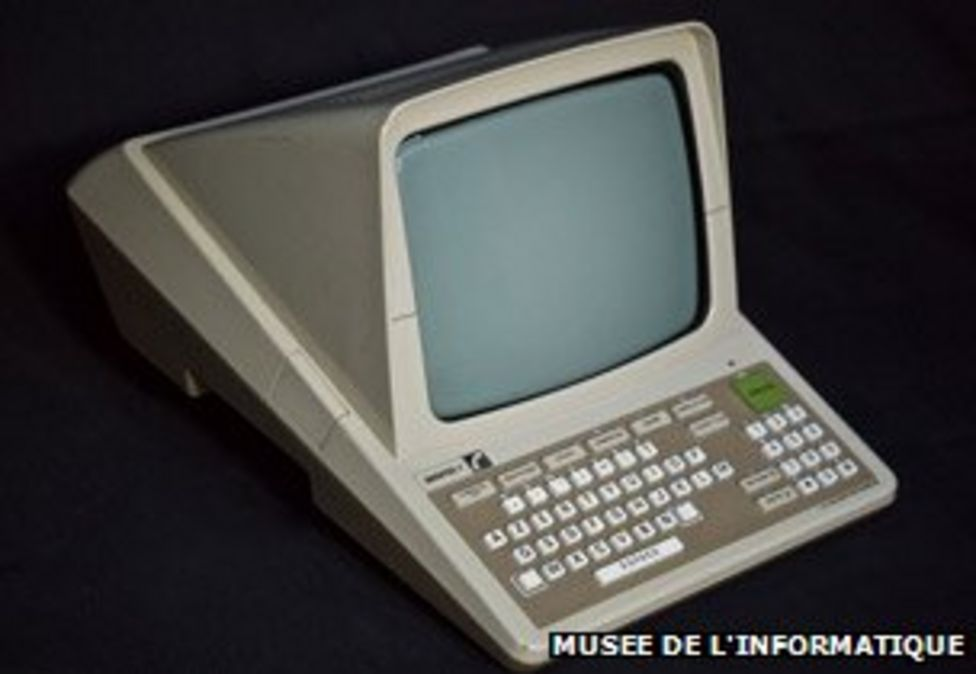
\includegraphics[width=1.0\linewidth]{../../imagens/minitel.jpg}
                \caption{Imagem de um terminal Minitel.}
                \label{5d9a2782548e094108d5241aeff768916b33be6c}
\end{minipage}%
\hspace{0.5cm}
\end{figure}



O Judici\'ario brasileiro inaugurou os servi\c{c}os digitais para atendimento ao cidad\~ao, no in\'{\i}cio da d\'ecada de 90. Esse pioneirismo se deu com o uso de c\'odigos de barra para identifica\c{c}\~ao de eleitores, por exemplo. Ali\'as, muito antes das a\c{c}\~oes do executivo, houve o desenvolvimento do sistema da Urna Eletr\^onica, uma iniciativa totalmente estatal, com a participa\c{c}\~ao de unidades de pesquisa federais  (MAMMANA et al., 1990) e (ANDRADE, 2022). As a\c{c}\~oes do executivo brasileiro em dire\c{c}\~ao ao governo eletr\^onico remontam a d\'ecada de 90, sempre com a participa\c{c}\~ao do SERPRO - Servi\c{c}o Federal de Processamento de Dados. Pode-se considerar que o programa de imposto de renda oferecido pela Receita Federal, a partir de, 1991 foi uma das primeiras a\c{c}\~oes em grande escala do Executivo no sentido de ofertar servi\c{c}os digitais diretos para o cidad\~ao, mesmo considerando que o envio dos dados da declara\c{c}\~ao por internet, s\'o foi viabilizado a partir de 1998. No in\'{\i}cio, era preciso enviar os disquetes da declara\c{c}\~ao, juntamente com a documenta\c{c}\~ao em papel.












O governo eletr\^onico ganhou mais institucionalidade no final do governo FHC, principalmente com a atua\c{c}\~ao de Pedro Parente \`a frente da Casa Civil  (DINIZ, 2009).












O movimento do Brasil em dire\c{c}\~ao ao Governo Eletr\^onico se deu no contexto da j\'a mencionada tend\^encia mundial de promover Reformas Administrativas da d\'ecada de 90 e in\'{\i}cio dos anos 2000. Ramon Garcia identifica a concomit\^ancia da a\c{c}\~ao de Brasil, M\'exico e Estados Unidos, que em tr\^es anos formalizaram seus programas de Governo Digital. Brasil e M\'exico focalizaram na infraestrutura da Internet, ao passo que os Estados Unidos trabalharam para o uso da internet em servi\c{c}os e processos.












O Governo Digital no Brasil foi formalizado por Decreto Presidencial, de 3 abril, de 2000  (DINIZ, 2009), cuja implementa\c{c}\~ao se deu sob a coordena\c{c}\~ao pol\'{\i}tica da Presid\^encia da Rep\'ublica, com apoio t\'ecnico e gerencial da Secretaria de Log\'{\i}stica e Tecnologia da Informa\c{c}\~ao (SLTI), do Minist\'erio do Planejamento, Or\c{c}amento e Gest\~ao. Essa atua\c{c}\~ao foi sustentada por um comit\^e, integrado pelos secret\'arios executivos (e cargos equivalentes) dos minist\'erios e \'org\~aos da Presid\^encia da Rep\'ublica, denominado Comit\^e Executivo de Governo Eletr\^onico (CEGE).












Inicialmente, o governo brasileiro concentrou esfor\c{c}os em tr\^es linhas de a\c{c}\~ao do Programa Sociedade da Informa\c{c}\~ao, institu\'{\i}do pelo Decreto no. 3.294, de 15 de dezembro, de 1999 (e depois alterado por v\'arios instrumentos legais): universaliza\c{c}\~ao de servi\c{c}os, governo ao alcance de todos e infraestrutura avan\c{c}ada.












As iniciativas do Governo FHC eram  acess\'{\i}veis a uma elite de cidad\~aos, uma vez que a maior parte da popula\c{c}\~ao n\~ao tinha acesso \`a internet, como se v\^e no estudo SIDRA do IBGE (apud Schmitz et al., 2021); e, embora ainda n\~ao houvesse um apontamento de solu\c{c}\~oes sist\^emicas para sua universaliza\c{c}\~ao, essas iniciativas abriram o caminho institucional do Governo Eletr\^onico.












\subsection[Pol\'{\i}ticas P\'ublicas de Inclus\~ao e Cultura Digital]{Pol\'{\i}ticas P\'ublicas de Inclus\~ao e Cultura Digital}\label{Pol\'{\i}ticas P\'ublicas de Inclus\~ao e Cultura Digital}
As transforma\c{c}\~oes, pelas quais a sociedade passava no in\'{\i}cio dos anos 90, exigiam novos paradigmas sociais, culturais e educacionais, que envolvessem estrat\'egias de inclus\~ao dos  cidad\~aos \`a nova realidade.












Entretanto, essa diretriz n\~ao estava presente na fase de implanta\c{c}\~ao do governo eletr\^onico no Brasil, ainda no Governo FHC. Inicialmente, tratando os cidad\~aos como clientes, o foco era a redu\c{c}\~ao de custos unit\'arios, melhorias na gest\~ao e qualidade dos servi\c{c}os p\'ublicos, transpar\^encia governamental e simplifica\c{c}\~ao de procedimentos - formalizados como estrat\'egias, macro-objetivos e  as metas priorit\'arias  do governo brasileiro para o per\'{\i}odo de 2000 a 2003.












Paralelamente, ocorria a consolida\c{c}\~ao de uma cadeia produtiva mundial de eletroeletr\^onicos eficiente, que usufru\'{\i}a de m\~ao de obra barata na \'Asia. Esse fato contribuiu para a redu\c{c}\~ao de barreiras econ\^omicas e para o acesso a dispositivos digitais, uma vez que houve ampla comoditiza\c{c}\~ao da produ\c{c}\~ao de eletroeletr\^onicos em geral e dos bens de computa\c{c}\~ao em particular. Esse fen\^omeno era uma decorr\^encia direta da Lei de Moore (CIPOLI, 2012), atrav\'es do qual o mundo passou a produzir mais transistores eletr\^onicos do que gr\~aos de soja, com ganhos de escala que tornaram essas tecnologias mais acess\'{\i}veis.












Vale lembrar que a Lei de Moore foi observada empiricamente, pela primeira vez, por Gordon Earle Moore, presidente da fabricante de microprocessadores Intel, em 1965. Ele observou que a cada 18 meses a ind\'ustria de microchips eletr\^onicos conseguia dobrar a quantidade de transistores presentes numa pastilha de sil\'{\i}cio de \'area definida. Os transistores s\~ao os \textquotedbl\{\}tijolos\textquotedbl\{\} da eletr\^onica e s\~ao usados para processar os sinais digitais.












Essa alta disponibilidade de equipamentos digitais, a relativo baixo custo, facilitou uma presen\c{c}a cada vez maior da internet na vida das pessoas, principalmente a partir da populariza\c{c}\~ao dos celulares do tipo \textquotedbl\{\}smartphone\textquotedbl\{\}, situa\c{c}\~ao que se reproduziu no Brasil no in\'{\i}cio do s\'eculo XXI.












A transforma\c{c}\~ao digital estimulou os governos a enfrentarem as dificuldades  de falta de  capacita\c{c}\~ao dos cidad\~aos na apropria\c{c}\~ao tecnol\'ogica, de forma que pudessem usufruir melhor o acesso aos equipamentos digitais. Para isso, estabeleceram pol\'{\i}ticas p\'ublicas que os preparassem para usufru\'{\i}rem do direito humano \`a comunica\c{c}\~ao, como estabelecido no Art. 19 da Declara\c{c}\~ao Universal de Direitos Humanos. Ou seja, os governos passaram a se preocupar com a inser\c{c}\~ao efetiva de seus cidad\~aos na Sociedade da Informa\c{c}\~ao.












Essas iniciativas ficaram conhecidas como programas pertinentes a politicas de \textquotedbl\{\}inclus\~ao digital ou  de \textquotedbl\{\}cultura digital\textquotedbl\{\}; ou mesmo de \textquotedbl\{\}alfabetiza\c{c}\~ao tecnol\'ogica\textquotedbl\{\}. Independentemente da abordagem escolhida, dentre as tr\^es indicadas, essas pol\'{\i}ticas sempre estiveram vinculadas \`as iniciativas de educa\c{c}\~ao.












Diferentes iniciativas e perspectivas foram implementadas para uso das tecnologias da informa\c{c}\~ao e comunica\c{c}\~ao no Brasil, na primeira d\'ecada deste s\'eculo, ao longo do segundo mandato de FHC, e do primeiro e segundo mandatos de Lula. Por meio de diferentes pol\'{\i}ticas p\'ublicas, foram disponibilizados acesso, equipamentos, aplicativos, softwares, hardwares, os quais visavam processar, armazenar, comunicar, prover apropria\c{c}\~ao tecnol\'ogica e acesso \'a informa\c{c}\~ao e ao conhecimento.












Dentre as pol\'{\i}ticas de inclus\~ao digital do per\'{\i}odo, destaca-se o  PROINFO - (Programa Nacional de Tecnologia Educacional) pol\'{\i}ticas de implanta\c{c}\~ao de \textquotedbl\{\}laborat\'orios de microcomputadores\textquotedbl\{\} em escolas p\'ublicas, iniciada no Governo FHC e, substancialmente, ampliada nos Governos de Lula e Dilma.












Tamb\'em, destacam-se as pol\'{\i}ticas com vi\'es industrial, voltadas para a redu\c{c}\~ao de pre\c{c}o dos computadores para consumidores finais; concomitantemente com a ado\c{c}\~ao de Software Livre, a exemplo do PC Conectado e o Computador para Todos.












A dissemina\c{c}\~ao de Telecentros, tamb\'em, teve um papel importante, criando pontos de acesso coletivo, que usufru\'{\i}am do Programa GESAC, quando necess\'ario.












Para garantir a objetividade da an\'alise, h\'a que se concentrar nos aspectos pertinentes ao objeto de estudo, i.e. o Programa WASH. Esta restri\c{c}\~ao exige focalizar a rela\c{c}\~ao entre as tecnologias digitais e a educa\c{c}\~ao, abordagem adotadas pelo programa em estudo, como se ver\'a mais adiante.












Assim, no prop\'osito de manter a objetividade e por sua rela\c{c}\~ao direta na g\^enese do Programa WASH, optou-se por focalizar, neste estudo:













\begin{alineas}
\item a) pol\'{\i}tica p\'ublica \textquotedbl\{\}Governo Eletr\^onico de Servi\c{c}os de Atendimento ao Cidad\~ao-GESAC\textquotedbl\{\}, criada em 2001, programa do Minist\'erio das Comunica\c{c}\~oes do governo FHC, cujo formato de interesse para este trabalho \'e o que se consolidou a partir de 2003;

\item b) Programa de Inclus\~ao Digital da Secretaria de Inclus\~ao Digital do Minist\'erio de Ci\^encia e Tecnologia, no recorte de 2005 a 2007; e
\item c) o Projeto Um Computador por Aluno (UCA), resultado da \textquotedbl\{\}tropicaliza\c{c}\~ao\textquotedbl\{\} da proposta americana \textquotedbl\{\}One Laptop per Child\textquotedbl\{\}.
\end{alineas}

Mesmo reconhecendo que este \'e um cap\'{\i}tulo de Fundamenta\c{c}\~ao Te\'orica, parece-nos oportuno abrir par\^enteses para contextualizar o que vem sendo descrito at\'e aqui, pela \'otica da experi\^encia profissional da autora. Nessa toada, cabe antecipar algo que ser\'a bastante enfatizado adiante: tivemos um papel na constru\c{c}\~ao e execu\c{c}\~ao de pol\'{\i}ticas p\'ublicas com as caracter\'{\i}sticas acima, inicialmente no \^ambito do Governo Eletr\^onico, passando pelas \'areas de comunica\c{c}\~ao, sa\'ude, cultura, e culminando na \'area de ci\^encia e tecnologia.












Estes trabalhos se deram em v\'arios momentos da carreira da autora, ao longo de quase tr\^es d\'ecadas. Isso a transformou em testemunhas ocular dos fatos, inicialmente no  munic\'{\i}pio de Campinas, na d\'ecada de 90, e, em seguida, no \^ambito do Governo Federal, nas primeiras duas d\'ecadas do presente s\'eculo.












Nessa trajet\'oria, foi poss\'{\i}vel aprender sobre as vantagens e desvantagens de cada uma das abordagens adotadas ao longo dessas tr\^es d\'ecadas, bem como sobre a forma de combinar capacita\c{c}\~ao e estabelecimento de infraestrutura para o acesso do cidad\~ao ao mundo digital.












A partir de uma pr\'atica regular e frequente de oficinas de forma\c{c}\~ao para  crian\c{c}as e adolescentes, que se iniciou em setembro de 2013, no Centro de Tecnologia da Informa\c{c}\~ao CTI - Renato Archer, em Campinas, esse aprendizado se consolidou em um m\'etodo, do qual essa pesquisadora \'e co-autora, conhecido como WASH.












Ap\'os um longo per\'{\i}odo de matura\c{c}\~ao, ajustes e repeti\c{c}\~ao, esse m\'etodo veio a ser formalizado em 2018, por meio de portaria de uma unidade de pesquisa do Minist\'erio da Ci\^encia, Tecnologia e Inova\c{c}\~oes (Portaria 178/2018 SEI/CTI).












A descri\c{c}\~ao detalhada do m\'etodo consta como anexo da referida portaria, a qual sintetiza os aprendizados conquistados ao longo dos anos, pelos v\'arios participantes do Programa. De 2018 para c\'a, mais aprendizados ocorreram, havendo uma necessidade de aprimoramento de sua caracteriza\c{c}\~ao.












\'E justamente uma an\'alise sobre esse m\'etodo que a presente disserta\c{c}\~ao intenciona oferecer, complementada por uma proposta de melhoria, na forma de produto educacional, como parte dos requisitos para obten\c{c}\~ao do t\'{\i}tulo de mestre, no \^ambito do Mestrado Profissional em Ensino de Ci\^encias Humanas, Sociais e da Natureza da Universidade  Tecnol\'ogica Federal do Paran\'a - UTFPR- Campus Londrina/PR.












\subsection[O pensamento de Papert]{O pensamento de Papert}\label{O pensamento de Papert}
Pela import\^ancia do pensamento de Papert para o Projeto One Laptop per Child (OLPC) e, portanto, para a g\^enese do WASH, cabe uma revis\~ao r\'apida de sua obra e contribui\c{c}\~oes, permitindo uma melhor compreens\~ao da inser\c{c}\~ao do WASH no universo conceitual das correntes pedag\'ogicas. Essa rela\c{c}\~ao entre a g\^enese do WASH e a proposta do OLPC ficar\'a mais clara no cap\'{\i}tulo de Resultados e An\'alise, quando a hist\'oria do WASH ser\'a apresentada. Por ora, \'e oportuno restringirmos-nos \`a revisita\c{c}\~ao das contribui\c{c}\~oes de Papert.












Para conhecer  o pensamento, um pouco da hist\'oria de Papert e  a filosofia do LOGO, \'e preciso fazer uma viagem no tempo, retornando a meados da d\'ecada de 60, quando o matem\'atico e educador sul-africano, radicado nos EUA, Seymour Papert, em colabora\c{c}\~ao com outros pesquisadores, desenvolveu a linguagem  de programa\c{c}\~ao LOGO.  Foi um dos fundadores do Media Lab e diretor do grupo de Epistemologia e Aprendizado do Massachusetts Institute of Technology - MIT.












Vale ressaltar para os nativos digitais, pessoas que nasceram a partir dos anos 80 e que cresceram com essas tecnologias, que no in\'{\i}cio da era da computa\c{c}\~ao, nos anos 60, os computadores existentes eram gigantes e ocupavam andares de pr\'edios. Eram usados apenas por grandes empresas e governos e n\~ao se cogitava aplic\'a-los para o uso pessoal e dom\'estico. Poucas pessoas, com treinamento, conseguiam usar um computador. O mouse, por exemplo, nem existia ainda. Para entrar com informa\c{c}\~oes nos computadores, era preciso usar cart\~oes perfurados, inspirados nos que foram criados pelo mec\^anico franc\^es Joseph-Marie Jacquard (1752-1854), que tamb\'em inventou o primeiro tear automatizado, cujos padr\~oes eram definidos nos cart\~oes perfurados.












Papert foi um pensador vision\'ario. Percebeu o potencial do uso da tecnologia na educa\c{c}\~ao. Fil\'osofo e pioneiro no pensar o processo de aprendizagem de crian\c{c}as, de forma diferente. Em 1968, escreveu o artigo \textquotedbl\{\}Teaching Children Thinking\textquotedbl\{\}, no qual abordou a tem\'atica crian\c{c}as, educa\c{c}\~ao e computadores:













\noindent\begin{center}\mbox{\centering\fbox{\centering\par\parbox{0.7\linewidth}{\small\textit{\textquotedbl\{\}T\'{\i}nhamos a certeza de que, quando os computadores se tornassem t\~ao comuns quanto o l\'apis, a educa\c{c}\~ao mudaria t\~ao r\'apida e profundamente quanto as transforma\c{c}\~oes pelas quais viv\'{\i}amos nos direitos civis e nas rela\c{c}\~oes sociais e sexuais\textquotedbl\{\}. (PAPERT, 1980)}\normalsize}}}\end{center}


Ele formulou esse pensamento quando os computadores dos anos 70 eram inacess\'{\i}veis tamb\'em para o sistema educacional. Naquele tempo, n\~ao existia o conceito de \textquotedbl\{\}microcomputadores\textquotedbl\{\} e os computadores existentes eram poucos, grandes, espalhados  (SOLOMON et al., 2020) e desajeitados, com poder de processamento e armazenagem entre milhares e milh\~oes de vezes, inferiores ao de um notebook. Mesmo com esse baixo desempenho, os custos eram muito altos e, portanto, o acesso era muito restrito. Entretanto, valendo-se de mainframes centralizados (computadores de grande porte) com as limita\c{c}\~oes indicadas, foi poss\'{\i}vel a Papert realizar incurs\~oes pioneiras no campo da aprendizagem para crian\c{c}as, utilizando os computadores que estavam dispon\'{\i}veis, ainda que esse uso estivesse restrito a uma elite, sem a possibilidade de uma grande dissemina\c{c}\~ao no sistema educacional.












Toda uma gera\c{c}\~ao de educadores foi formada em torno das ideias de Papert, que defendia que a aprendizagem de linguagem de programa\c{c}\~ao de computadores, j\'a no ensino fundamental, poderia ter um papel importante no aprendizado de muitas outras disciplinas tradicionais, principalmente a matem\'atica, mas tamb\'em gram\'atica (SOLOMON et al., 2020), entre outras.












Entendemos que a proposta de Papert, at\'e por enfatizar o aprendizado de crian\c{c}as, n\~ao tinha qualquer ambi\c{c}\~ao de capacita\c{c}\~ao profissional e, por si, n\~ao visava diretamente fazer frente aos desafios do \textquotedbl\{\}mundo do trabalho\textquotedbl\{\}, que foram sendo introduzidos pelas transforma\c{c}\~oes inerentes \`a Sociedade da Informa\c{c}\~ao, nas d\'ecadas subsequentes.












Em sua obra \textquotedbl\{\}A M\'aquina das Crian\c{c}as\textquotedbl\{\} (1994), Papert discorre sobre a import\^ancia da tecnologia e sua inser\c{c}\~ao na educa\c{c}\~ao, a fim de melhorar a qualidade do ambiente de aprendizagem.













\noindent\begin{center}\mbox{\centering\fbox{\centering\par\parbox{0.7\linewidth}{\small\textit{N\'os podemos dar um poder sem precedentes para as crian\c{c}as inventarem e desenvolverem projetos excitantes, provendo o acesso a computadores, com uma linguagem de programa\c{c}\~ao adequada, intelig\'{\i}vel e clara, bem como com perif\'ericos capazes de produzir uma a\c{c}\~ao on-line/real-time\textquotedbl\{\}  (SOLOMON et al., 2020).}\normalsize}}}\end{center}


Segundo o autor, \textquotedbl\{\}ao redor do mundo inteiro, as crian\c{c}as entraram em um apaixonante e duradouro caso de amor com os computadores\textquotedbl\{\} (1994, p.07).












Essa filosofia e a maneira de colocar em pr\'atica a crian\c{c}a epistem\'ologa vieram do seu aprendizado na rela\c{c}\~ao de trabalho e conviv\^encia com Piaget.












Papert ficou impressionado de ver as crian\c{c}as, construtoras de suas pr\'oprias estruturas intelectuais [Logo, computadores e educa\c{c}\~ao, p\'ag 35]:













\noindent\begin{center}\mbox{\centering\fbox{\centering\par\parbox{0.7\linewidth}{\small\textit{A linguagem LOGO faz com que o computador deixe de ser apenas um meio de transferir informa\c{c}\~ao e passe a ser a ferramenta, com a qual a crian\c{c}a pode formalizar os seus conhecimentos intuitivos.  (PAPERT, 1980)}\normalsize}}}\end{center}


Essa nova rela\c{c}\~ao com a computa\c{c}\~ao, proposta por Papert, permitiu uma transforma\c{c}\~ao na educa\c{c}\~ao e no processo de ensino e aprendizagem, colocando o computador como relevante para o ensino fundamental, mas sempre entendendo a crian\c{c}a como programadora e n\~ao apenas como usu\'aria.












Papert examinou as crian\c{c}as que tinham aprendido a programar computadores e identificou que elas podiam usar os modelos concretos para \textquotedbl\{\}pensar sobre o pensar\textquotedbl\{\} e \textquotedbl\{\}aprender sobre o aprender\textquotedbl\{\}  (PAPERT, 2005), estimulando-as  a aumentarem seus poderes de epistem\'ologos. Sobre isso, ele discorreu no artigo publicado, em 1970, intitulado Teaching Children Thinking.












Segundo Jos\'e Armando Valente, um dos respons\'aveis, em conjunto com a Professora Afira Vianna Ripper, pela tradu\c{c}\~ao do livro LOGO: computadores e educa\c{c}\~ao: \textquotedbl\{\}Papert acreditava que o computador era a ferramenta que propiciava \`as crian\c{c}as as condi\c{c}\~oes de entrar em contato com algumas das mais profundas ideias em ci\^encia, matem\'atica e a cria\c{c}\~ao de modelos\textquotedbl\{\}.












Programar, na filosofia LOGO, significa \textquotedbl\{\}comunicar-se com o computador, numa linguagem que tanto ele, quanto o homem,  podem entender\textquotedbl\{\}. Toda crian\c{c}a aprende a falar. Por que, ent\~ao, n\~ao deveria aprender a \textquotedbl\{\}falar\textquotedbl\{\} com um computador?\textquotedbl\{\}, indagava Papert  (PAPERT, 1980).












A proposta de Papert envolvia, tamb\'em, a ideia de que o computador pudesse ser um interlocutor  de matem\'atica ou um interlocutor de l\'{\i}nguas. Nessa concep\c{c}\~ao, o LOGO, ao ser um interlocutor da matem\'atica, contribui, de uma maneira l\'udica, para superar as barreiras matof\'obicas (fobia por matem\'atica e fobia pelo aprendizado), transformando a matem\'atica, que passa a ser uma l\'{\i}ngua viva  (PAPERT, 1980) .












Papert abordou sobre a \textquotedbl\{\}matofobia: o medo de aprender\textquotedbl\{\}, com duas associa\c{c}\~oes: o conhecido medo da matem\'atica, que tem a intensidade de uma verdadeira fobia; e o  significado do radical mathe, que, em grego, significa aprender.













\noindent\begin{center}\mbox{\centering\fbox{\centering\par\parbox{0.7\linewidth}{\small\textit{\textquotedbl\{\}A matofobia pode cultural e materialmente limitar a vida das pessoas. Muitas outras pessoas ainda n\~ao desistiram completamente de aprender, mas sentem-se impedidas por opini\~oes negativas, arraigadas sobre suas capacidades. A defici\^encia torna-se uma identidade, \textquotedbl\{\}n\~ao consigo aprender franc\^es, n\~ao tenho ouvido para l\'{\i}nguas, nunca poderia ser um homem de neg\'ocios, n\~ao tenho cabe\c{c}a para contas. Essas cren\c{c}as s\~ao supersti\c{c}\~oes e est\~ao presentes em nosso cotidiano, elas criam tabus para a aprendizagem. Se as pessoas acreditam que n\~ao podem entender matem\'atica, conseguiram abster-se de tentar executar qualquer coisa que reconhe\c{c}am a matem\'atica, gerando como consequ\^encia uma auto-sabotagem\textquotedbl\{\}  [LOGO: Computadores e educa\c{c}\~ao, PAPERT, S. pg.62, 63]}\normalsize}}}\end{center}


Papert chamou aten\c{c}\~ao quanto \`a separa\c{c}\~ao, imposta por nossa cultura, entre o verbal e o matem\'atico. Tornou-se muito comum falar como se houvesse diferentes c\'erebros ou mesmo \'org\~aos separados no c\'erebro, para matem\'atica e linguagem.












Em suas viv\^encias com as crian\c{c}as, Papert materializava o pensamento abstrato da matem\'atica. Ao constru\'{\i}rem os seus jogos, primeiro, as crian\c{c}as faziam o movimento com o seu corpo, para, depois, usar os comandos do LOGO. A ilustra\c{c}\~ao deste processo pode ser vista no v\'{\i}deo  da entrevista, realizada com a Professora Afira Ripper,  um dos produtos desta disserta\c{c}\~ao (ver no cap\'{\i}tulo de Produtos Educacionais).












As crian\c{c}as s\~ao permeadas por ideias de que h\'a pessoas boas em matem\'atica e outras que n\~ao podem entender matem\'atica; mas, Papert acreditava que a presen\c{c}a do computador poderia neutralizar a matofobia  (PAPERT, 1980) .












Papert criticou o modo como os computadores estavam sendo usados na educa\c{c}\~ao americana, ou seja, estavam sendo usados para fornecer informa\c{c}\~oes ou instrumentos de instru\c{c}\~ao assistida por computador (CAI – Computed Aid instruction)  (PAPERT, 2005a).












Segunda a percep\c{c}\~ao do autor, o tipo de abordagem existente materializava a ideia do computador programando a crian\c{c}a (PAPERT, 2005a). O LOGO, enquanto linguagem de programa\c{c}\~ao pensada para as crian\c{c}as, tinha como proposta inverter essa rela\c{c}\~ao.












Papert p\^ode conferir, com as crian\c{c}as em idade pr\'e-escolar, que \'e poss\'{\i}vel ela controlar a m\'aquina e ser protagonista na programa\c{c}\~ao do seu computador. Com isso, ao ensinar o computador a pensar, ela explora a sua pr\'opria forma de pensar.












Teaching Children Thinking, artigo escrito por Papert, foi a primeira publica\c{c}\~ao que sugeria que a crian\c{c}a poderia ficar no comando da m\'aquina e n\~ao a m\'aquina no comando da crian\c{c}a.  Esse artigo  foi publicado em 1970; e,  apresentou um novo processo para a educa\c{c}\~ao, em que os computadores pudessem serem usados para a criatividade.












Papert apresentou uma nova ideia: de que \textquotedbl\{\}ensinar o pensamento\textquotedbl\{\}  \'e apropriado para a escola prim\'aria, mas essa n\~ao era a corrente principal da educa\c{c}\~ao americana, naquele contexto.












O LOGO, segundo Papert, proporcionou a milhares de professores do ensino b\'asico a sua primeira oportunidade para apropriar-se do computador, de maneira que ampliaram seus estilos pessoais de ensinar. ( Papert, S, \textquotedbl\{\}A maquina das crian\c{c}as, repensando a escola da era da inform\'atica\textquotedbl\{\}, pg57).












Em seu percurso de pesquisa, na apresenta\c{c}\~ao do LOGO, na experimenta\c{c}\~ao, seja com as crian\c{c}as ou com os professores, Papert encontrou o que ele chamava de \textquotedbl\{\}professores conservadores e  inovadores\textquotedbl\{\} (PAPERT, 1980).












Outro aspecto importante na obra e viv\^encia de Papert \'e quanto aos modos hier\'arquicos de pensar sobre o conhecimento. Ele adotou o termo  \textquotedbl\{\} heterarquia \textquotedbl\{\} para descrever a forma de aprendizagem pretendida, um conceito presente em  \textquotedbl\{\}A m\'aquina das Crian\c{c}as\textquotedbl\{\}. Trata-se de  um termo oposto \`a hierarquia, comum na forma de trabalho da escola tradicional. Como vimos na se\c{c}\~ao 2.1.2, na heterarquia, cada elemento \'e igualmente governado por todos os outros.












Mais adiante ser\'a poss\'{\i}vel mostrar que o WASH se estruturou numa forma de heterarquia, assunto que ser\'a tratado nos resultados.












A proposta de Papert para o Governo Federal, em 2005, n\~ao foi a primeira oportunidade de intera\c{c}\~ao com o poder p\'ublico brasileiro.












Em 1989, quando a prefeita eleita Luiza Erundina de Souza assumiu a Prefeitura de S\~ao Paulo, convidou o Prof. Paulo Freire para assumir a pasta de educa\c{c}\~ao. Um novo projeto pol\'{\i}tico-educacional foi elaborado a partir de uma reavalia\c{c}\~ao dos existentes. A partir dessa iniciativa, foi recriado o projeto de Educa\c{c}\~ao e Inform\'atica da Secretaria Municipal de Educa\c{c}\~ao de S\~ao Paulo, fundamentando-se na tese de que:













\noindent\begin{center}\mbox{\centering\fbox{\centering\par\parbox{0.7\linewidth}{\small\textit{[…] uma sociedade informatizada est\'a passando a exigir homens com potencial de assimilar a \textquotedbl\{\}novidade\textquotedbl\{\} e criar o novo, o homem aberto para o mundo, no sentido que lhe confere a teoria piagetiana quando se refere \`as assimila\c{c}\~oes mentais majorantes; da mesma forma, exige a presen\c{c}a do cidad\~ao cr\'{\i}tico e comunit\'ario, onde os artefatos tecnol\'ogicos, especificamente o computador, possam ser ferramentas auxiliares para a constru\c{c}\~ao de uma sociedade mais igualit\'aria e justa. (S\~AO PAULO, 1992 , p. 7). Em 1995, Paulo Freire.}\normalsize}}}\end{center}


Ao longo da consolida\c{c}\~ao dos conceitos descritos at\'e aqui, Papert estabeleceu uma vertente do construcionismo com grandes resultados pr\'aticos, tendo inaugurado a base para uma cultura de aprendizagem baseada no \textquotedbl\{\}fazer\textquotedbl\{\}, sustentada em ideias como:













\begin{alineas}
\item A crian\c{c}a deve estar no centro do processo de aprendizagem, conduzindo-na sempre que poss\'{\i}vel;
\item N\~ao existe idade ideal para aprender as coisas: cada crian\c{c}a tem o seu pr\'oprio tempo e momento de interesse; e
\item Das pr\'oprias palavras de Papert: \textquotedbl\{\}a meta \'e ensinar de forma a produzir a maior aprendizagem, a partir do m\'{\i}nimo de ensino\textquotedbl\{\}  (PAPERT, 1994).
\end{alineas}

Com estes conceitos, Papert indica a necessidade de estimular as crian\c{c}as a fazerem suas pr\'oprias pescarias,  (PAPERT, 1994) com vistas a obter o conhecimento.












Complementam essas ideias,os conceitos de  (PAPERT, 1999):













\begin{alineas}
\item Learn by doing ou aprender fazendo: a ideia, em parte,  do senso comum em parte originada, por Dewey, \'e aprender ao longo do processo de fazer coisas que realmente nos causa interesse;
\item Technology as a building material, ou \textquotedbl\{\}tecnologia como um material de constru\c{c}\~ao\textquotedbl\{\}: a tecnologia nos permite fazer muito mais, \`a medida que aprendemos, porque ela nos empodera, com seus recursos, para alcan\c{c}ar caracter\'{\i}sticas em nossas produ\c{c}\~oes, seja um jogo, prot\'otipo ou pe\c{c}a de comunica\c{c}\~ao, por exemplo, que n\~ao conseguir\'{\i}amos sem ela;
\item Hard fun ou \textquotedbl\{\}divers\~ao desafiadora\textquotedbl\{\}: existe um entendimento de que aprende-se melhor quando nos divertimos, mas a divers\~ao n\~ao requer que a atividade seja f\'acil. \'E preciso garantir que a aprendizagem, mesmo sendo divertida, tenha um car\'ater de desafio, que instigue o educando.
\item Learn to learn ou \textquotedbl\{\}aprenda a aprender\textquotedbl\{\}: o conceito subjacente \'e o de protagonismo do educando na aprendizagem, implicando que a ideia de ensinar \'e muito menos importante do que a ideia de aprender.
\item Taking time ou \textquotedbl\{\}assumindo o controle do seu pr\'oprio tempo\textquotedbl\{\}: os estudantes devem, ao assumir o protagonismo de sua aprendizagem, gerenciar o pr\'oprio tempo e suas pr\'oprias atividades, sem a necessidade de algu\'em lhes dizendo o que fazer;
\item You can’t get it right without getting it wrong ou \textquotedbl\{\}voc\^e n\~ao consegue acertar
se n\~ao errar primeiro\textquotedbl\{\}\'e o conceito de que para aprender \'e preciso existir a
liberdade para errar. As coisas importantes nunca funcionam da primeira vez, e ao tentar corrig\'{\i}-las \'e que o processo de aprendizagem ocorre;
\item Do unto ourselves what we do unto our students ou \textquotedbl\{\}fa\c{c}amos conosco o que fazemos com nossos estudantes\textquotedbl\{\}: este conceito \'e direcionado aos educadores, que precisam adotar para si a ideia de que, tamb\'em, v\~ao aprender fazendo e tamb\'em v\~ao aprender errando. A melhor li\c{c}\~ao para nossos estudantes \'e deix\'a-los nos assistir, \textquotedbl\{\}sofrendo\textquotedbl\{\} durante o nosso pr\'oprio aprendizado;
\item We are entering a digital world ou \textquotedbl\{\}n\'os estamos entrando em um mundo digital\textquotedbl\{\}: conhecer e saber atuar dentro do mundo digital \'e t\~ao importante quando ler ou escrever.
\end{alineas}

Mitchel Resnick, do Grupo Lifelong Kindergarten, MIT, baseado nas ideias construcionistas de Seymour Papert, apresenta, em 2007, o Scratch, como uma ferramenta para a aprendizagem criativa, considerando os 4 Ps da aprendizagem criativa: projetos, paix\~ao, pares e pensar brincando (play). A iniciativa de Resnick se consolidou. \'E por isso que, hoje, voc\^e pode encontrar no Scratch um aliado no processo de aprendizagem. O Scratch re\'une uma comunidade ativa, da qual fazem parte quase 50 milh\~oes de crian\c{c}as, jovens e adultos do mundo inteiro. O coordenador do Programa WASH teve a oportunidade de conhecer uma das primeiras vers\~oes do Scratch, descrita pessoalmente pelo Prof. Resnick, 2007.












O Programa WASH, seguindo nossa hip\'otese de que tem g\^enese nas propostas do OLPC, se inspirou na metodologia subjacente ao Scratch e, desde os prim\'ordios, tem como base o uso desse instrumento nas atividades de educa\c{c}\~ao. O WASH estimula a cultura digital no turno e contraturno escolares e oferece oficinas, que n\~ao podem ser classificadas como aulas tradicionais, porque abdicam de roteiros, apostilas e conte\'udos fixos, uma caracter\'{\i}stica muito presente nos m\'etodos criados pelos pensadores do MIT, disc\'{\i}pulos de Papert. Nessa concep\c{c}\~ao, o educando aprende, fazendo e errando, com objetivos determinados e oportunidade para tentar de novo. Assim, embora haja uma abertura muito grande para a experimenta\c{c}\~ao de propostas variadas, o Programa WASH oferece, como linha b\'asica de a\c{c}\~ao, a programa\c{c}\~ao de jogos, usando a linguagem Scratch, e isto ser\'a visto adiante.












Ao usar o Scratch, nas oficinas do Programa WASH, estamos oportunizando e estimulando \textquotedbl\{\}as crian\c{c}as e jovens a serem criativas, produzirem seus jogos, suas narrativas, suas anima\c{c}\~oes, o racioc\'{\i}nio l\'ogico, contribuindo com o letramento digital, colaborando com a alfabetiza\c{c}\~ao cient\'{\i}fica, e para n\~ao serem somente consumidores de jogos, games, mas produtores, tamb\'em\textquotedbl\{\}.












Os resultados do emprego do Scratch, no Programa WASH ser\~ao discutidos em Resultados e An\'alise; mas pode-se antecipar que envolveram milhares de crian\c{c}as e jovens, produzindo jogos, com os bolsistas de inicia\c{c}\~ao cient\'{\i}fica aprendendo com o ensinar, multiplicando e compartilhando o conhecimento das ferramentas digitais  com a comunidade, tanto por meio das oficinas do WASH, quanto pela participa\c{c}\~ao em feiras, eventos e congressos.












Em nossa viv\^encia, a tartaruga, de Seymour Papert; e o gato, de Mitchel Resnick,  representam as bases da  programa\c{c}\~ao e com eles aprendemos a  programar, brincando.












\subsection[O LOGO e o SCRATCH]{O LOGO e o SCRATCH}\label{O LOGO e o SCRATCH}
O LOGO \'e uma linguagem de programa\c{c}\~ao, desenvolvida em 1966 por Seymour Papert, Wallace Feurzeig, Daniel Bobrow e Cynthia Solomon (ver Fig. 4), no \^ambito dos laborat\'orios Bolt, Beranek and Newman, Inc (BBN) and MIT Artificial Intelligence Lab (SOLOMON et al., 2020). O LOGO foi muito difundido no contexto educacional a partir daquela d\'ecada, tendo ajudado gera\c{c}\~oes de crian\c{c}as a aprender v\'arias disciplinas, mas principalmente matem\'atica  (SOLOMON et al., 2020).














\captionsetup{format=plain}
\begin{figure}[max size={\textwidth}{\textheight}]

\centering


\begin{minipage}[b]{0.4\linewidth}
        \centering
                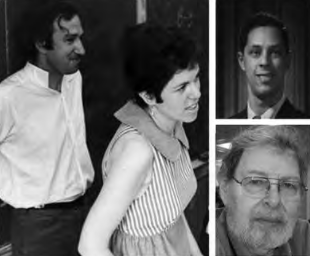
\includegraphics[width=1.0\linewidth]{../../imagens/criadores-logo.png}
                \caption{Criadores do Logo em 1966: Seymour Papert, Cynthia Solomon, Danny Bobrow e Wally Feurzeig (fonte:  [[SOLOMON et al. (2020)]])}
                \label{c40acbbf355efda753f44d02f297bbce67f5e4b8}
\end{minipage}%
\hspace{0.5cm}
\begin{minipage}[b]{0.4\linewidth}
        \centering
                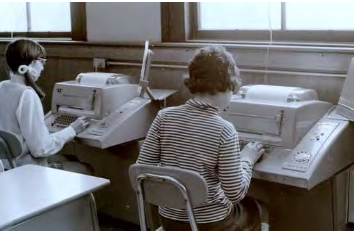
\includegraphics[width=1.0\linewidth]{../../imagens/criancas-1968.png}
                \caption{Crian\c{c}as de 12 anos da Muzzey Junior High School usando LOGO em terminais teletipo (Fonte:  [[SOLOMON et al. (2020)]], circa 1968).}
                \label{1a5368da06f895c87008b3fc1675ccfbb494f1f9}
\end{minipage}
\hspace{0.5cm}
\begin{minipage}[b]{0.4\linewidth}
        \centering
                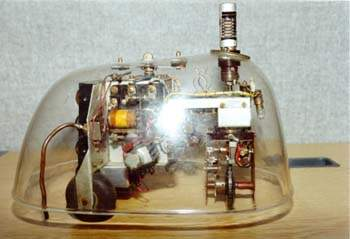
\includegraphics[width=1.0\linewidth]{../../imagens/Elmer-Elsie4.jpg}
                \caption{Elmer e Elsie eram dois rob\^os com rodas, chamados de c\'agados (tortoise), que podiam se deslocar pelo ch\~ao. Foram desenvolvidos pelo Ingl\^es Grey Walter.}
                \label{fdc1f0b8e99c3e3a345c88c79ff4e953d65b3424}
\end{minipage}%
\hspace{0.5cm}
\begin{minipage}[b]{0.4\linewidth}
        \centering
                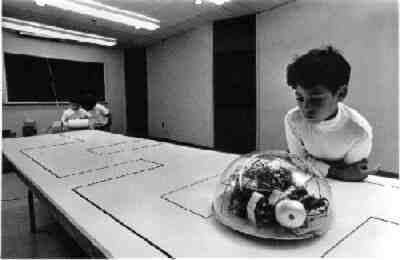
\includegraphics[width=1.0\linewidth]{../../imagens/historia-logo-turtle-01.jpg}
                \caption{Em foto de 1969, uma crian\c{c}a observa o primeiro rob\^o tartaruga criado no MIT (Fonte:  [[CIBERNECTZOO (2010)]]).}
                \label{c2ca828982a83621e08977a23628db7b32a934d9}
\end{minipage}
\hspace{0.5cm}
\begin{minipage}[b]{0.4\linewidth}
        \centering
                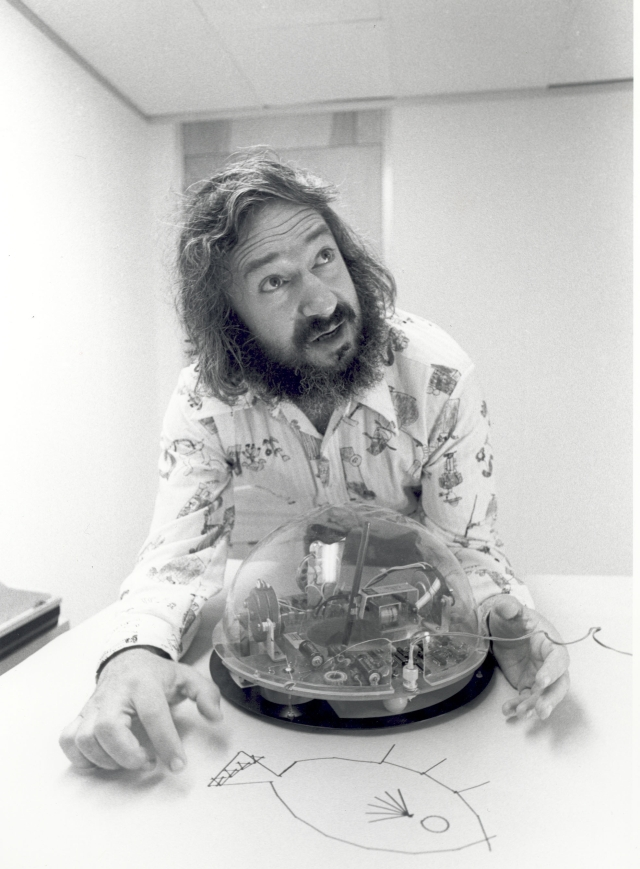
\includegraphics[width=1.0\linewidth]{../../imagens/Papert-x640.jpg}
                \caption{Papert com uma de suas tartarugas rob\^os. (Fonte:  [[CIBERNECTZOO (2010)]])}
                \label{16372e5cf76e6860245131e51a3bf17c58dd1e46}
\end{minipage}%
\hspace{0.5cm}
\begin{minipage}[b]{0.4\linewidth}
        \centering
                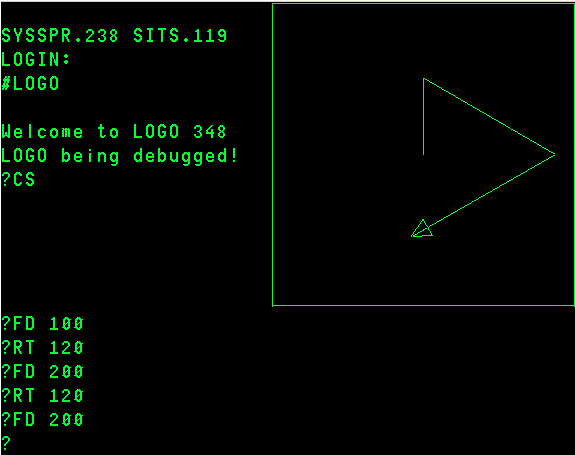
\includegraphics[width=1.0\linewidth]{../../imagens/logo-PDP11.png}
                \caption{Imagem de uma tela do LOGO num terminal gr\'afico da d\'ecada de 70, provavelmente rodando em um PDP11. O tri\^angulo pequeno \'e a tartaruga (Fonte: gunkies.org).}
                \label{ca83b217b58f57e503ff496c6c6f47bee5dc77cd}
\end{minipage}
\hspace{0.5cm}
\end{figure}



No LOGO, a constru\c{c}\~ao se d\'a pela cria\c{c}\~ao, jun\c{c}\~ao e reaproveitamento de algoritmos de computador, como num jogo de encaixe.












O LOGO possibilita a defini\c{c}\~ao de novos comandos e fun\c{c}\~oes, numa configura\c{c}\~ao interativa, que permite visualizar e vivenciar os resultados, \`a medida que os programas s\~ao constru\'{\i}dos. Considerando que o LOGO foi criado na d\'ecada de 60, j\'a se tratava de uma inova\c{c}\~ao num per\'{\i}odo em que a interface de muitos computadores ainda era baseada em cart\~ao perfurado.












Desta forma, pode-se dizer que o LOGO nunca foi um mero brinquedo; mas, ao contr\'ario, se constitui em uma poderosa linguagem de computa\c{c}\~ao, planejada para fornecer acesso \`a programa\c{c}\~ao para principiantes, visando estimular a aprendizagem.












O LOGO \'e associado \`a imagem de seu cursor, uma tartaruga que percorre a tela deixando um rastro que forma as figuras geom\'etricas desejadas. Entretanto, poucas pessoas sabem que em seu in\'{\i}cio, a linguagem \textquotedbl\{\}focava em brincar com palavras e senten\c{c}as\textquotedbl\{\} (SOLOMON et al., 2020), sendo que sua tartaruga \textquotedbl\{\} ic\^onica \textquotedbl\{\} apareceu depois.  SOLOMON et al. (2020) menciona que o aprendizado sem a tartaruga podia ocorrer no campo da gram\'atica, por exemplo, quando as crian\c{c}as, independentemente de recursos visuais, demonstravam uma aprecia\c{c}\~ao por sistemas formais.












A Fig. 5 mostra a experi\^encia de utiliza\c{c}\~ao do LOGO com alunos do s\'etimo ano na Escola Muzzey Junior High School, na cidade de Lexington, em Massachussetts. Naquela experi\^encia, os estudantes desenvolveram o jogo Pig Latin, Vinte Quest\~oes, Nim, SENGEN (gerador de senten\c{c}as), ensino de matem\'atica e contador de hist\'orias  (SOLOMON et al., 2020). Eram usados terminais teletipos sem tela e ainda n\~ao existia o conceito de tartaruga.












A ideia do \'{\i}cone da tartaruga surgiu quando a experi\^encia da Escola Muzzey estava chegando ao fim, em 1969. As crian\c{c}as tiveram uma boa experi\^encia com a diversidade de projetos de programa\c{c}\~ao, que focavam em palavras, e senten\c{c}as, ainda sem as tartarugas; mas Papert queria expandir os dom\'{\i}nios de explora\c{c}\~ao pelas crian\c{c}as (SOLOMON et al., 2020). Para isso, foi pensado que era necess\'ario criar um objeto concreto para se brincar, algo que pudesse ser controlado diretamente pelas crian\c{c}as. Papert se inspirou nos \textquotedbl\{\}c\'agados\textquotedbl\{\}  (tortoise) rob\^os de William Grey Walter. \textquotedbl\{\}Elmer and Elsie\textquotedbl\{\} (ver Fig. 6) tinham rodas, motores e sensores e podiam se deslocar pelo ch\~ao da sala ou sobre uma mesa, sendo conectados ao computador por um cabo (tether) num primeiro momento. Logo em seguida foram substitu\'{\i}dos pela imagem de tartarugas numa tela de computador, (SOLOMON et al., 2020). A Fig. 7 mostra uma crian\c{c}a de 1969 observando o primeiro rob\^o tartaruga criado no MIT, a Fig. 8 mostra Papert com uma de suas tartarugas e a Fig. 9 mostra a imagem de uma tela de um computador PDP11 rodando LOGO na d\'ecada de 70.












Com o avan\c{c}o da tecnologia e a disponibiliza\c{c}\~ao de interfaces humano-computador, cada vez mais avan\c{c}adas (displays melhores, mouse, tablets, etc.), o longevo LOGO come\c{c}ou a sentir o peso da idade.












Em SOLOMON et al. (2020) \'e mencionado o valor de uma alternativa ao LOGO, que pudesse tirar proveito das virtudes das chamadas \textquotedbl\{\}linguagens de programa\c{c}\~ao visual\textquotedbl\{\}, uma vez que reconheciam:













\noindent\begin{center}\mbox{\centering\fbox{\centering\par\parbox{0.7\linewidth}{\small\textit{\textquotedbl\{\}Os jovens iniciantes em LOGO dedicavam muito tempo ca\c{c}ando letras no teclado\textquotedbl\{\} (SOLOMON et al., 2020)}\normalsize}}}\end{center}


A alternativa veio na forma de linguagem Scratch, criada por Mitchel Resnick e seus estudantes. Mitchel, em 1989, j\'a tinha se dedicado ao desenvolvimento de uma vers\~ao do LOGO, com m\'ultiplas tartarugas (StarLogo). As discuss\~oes sobre a necessidade de um  LOGO visual come\c{c}aram logo depois, em 1990, mesmo com a vis\~ao de Papert que uso de uma interface visual significaria apenas uma mudan\c{c}a de representa\c{c}\~ao, o que n\~ao faria muita diferen\c{c}a   (SOLOMON et al., 2020). Mitchel Resnick, segundo  SOLOMON et al. (2020), \textquotedbl\{\}n\~ao compartilhava desse pessimismo\textquotedbl\{\} e pressionou para que uma linguagem em blocos simples fosse criada e testada. Sobre o teste,  SOLOMON et al. (2020) se manifesta como segue:













\noindent\begin{center}\mbox{\centering\fbox{\centering\par\parbox{0.7\linewidth}{\small\textit{\textquotedbl\{\}Para a minha surpresa, mas n\~ao para a surpresa de Mitchel, o teste funcionou realmente bem. O que Seymour e eu n\~ao t\'{\i}nhamos antecipado \'e que o fato da linguagem parecer simples aumentava a vontade das pessoas se engajarem nos est\'agios iniciais da experi\^encia de programa\c{c}\~ao, comparativamente com a forma n\~ao visual. Em certo sentido n\~ao era mais simples, mas o que importa \'e que parecia mais simples.  (SOLOMON et al., 2020, tradu\c{c}\~ao livre)}\normalsize}}}\end{center}


Assim, depois de uma s\'erie de desdobramentos e desenvolvimentos, Mitchel Resnick apresenta, em 2007, o Scratch, como uma ferramenta para a aprendizagem criativa. A iniciativa de Resnick se consolidou, criando as condi\c{c}\~oes para que fosse disponibilizada uma ferramenta poderosa de programa\c{c}\~ao, encapsulada num formato l\'udico e atraente para crian\c{c}as, que funciona como um aliado no processo de aprendizagem. A Fig. 10 mostra um trecho de c\'odigo em Scratch, organizado na forma de blocos.














\captionsetup{format=plain}
\begin{figure}[max size={\textwidth}{\textheight}]

\centering


\begin{minipage}[b]{0.4\linewidth}
        \centering
                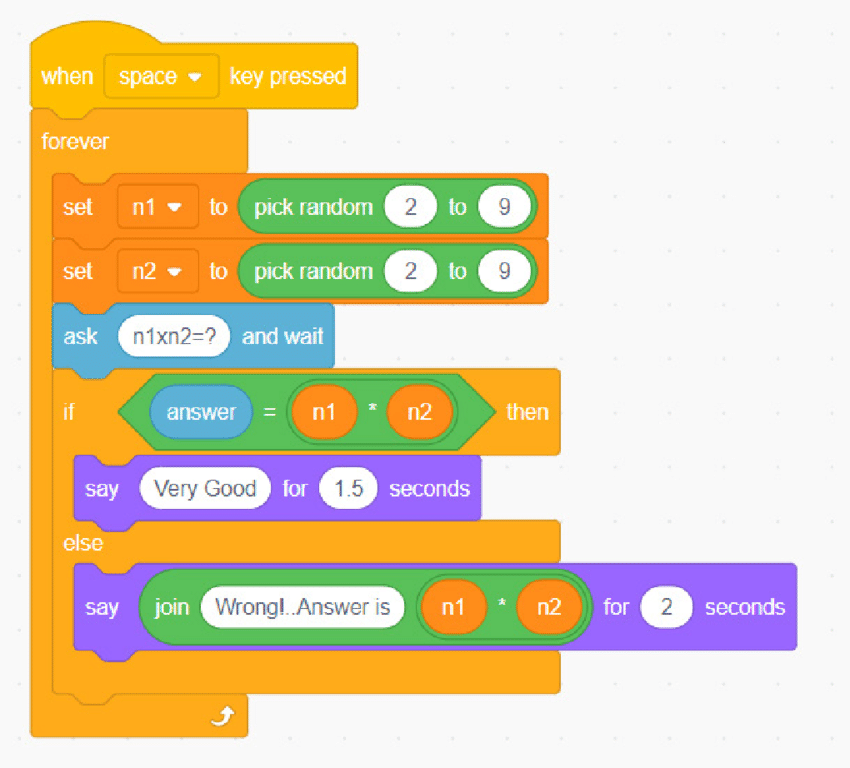
\includegraphics[width=1.0\linewidth]{../../imagens/Scratch-Block.png}
                \caption{Trecho de um c\'odigo em Scratch, em que se v\^e a organiza\c{c}\~ao por blocos, que podem ser montados como num jogo de encaixe. (Fonte: u [[SUNG (2019)]])}
                \label{5cac9c9edeb34a88b5571069bb494cda1ce1bd9c}
\end{minipage}%
\hspace{0.5cm}
\end{figure}



O Scratch re\'une uma comunidade ativa, da qual fazem parte quase 50 milh\~oes de crian\c{c}as, jovens e adultos do mundo inteiro. O Coordenador do Programa WASH teve a oportunidade de conhecer uma das primeiras vers\~oes do Scratch, descrita pessoalmente pelo Prof. Resnick, na \'epoca de seu desenvolvimento.












Ainda h\'a questionamentos sobre a acessibilidade do Scratch, por seu car\'ater visual, cabendo aos pesquisadores do mundo todo se debrucem sobre a quest\~ao do design universal, para que pessoas cegas, principalmente, possam usufruir dos mesmos benef\'{\i}cios da ferramenta, que hoje est\'a restrita aos videntes.












\subsection[O que \'e STEM/STEAM?]{O que \'e STEM/STEAM?}\label{O que \'e STEM/STEAM?}
V\'arios autores (CATTERALL, 2017)  (GONZALES e KUENZI, 2012)  (JANKOSKI, 2017)  (BYBEE, 2010) indicam a d\'ecada de 90 do s\'eculo passado como o in\'{\i}cio do uso estruturado do conceito de Science, Technology, Engineering and Mathematics (STEM) em curr\'{\i}culos escolares, mas o acr\^onimo para represent\'a-lo teve altera\c{c}\~oes ao longo dos anos. 
Segundo post de  JANKOSKI (2017), inicialmente o conceito era representado pela sigla SMET, mas a similaridade de pron\'uncia com a palavra \textquotedbl\{\}smut (que significa obscenidade, em ingl\^es) sugeriu a mudan\c{c}a da sigla para METS e depois para STEM, em 2001  (BRITANNICA, 2022a).












Autores mencionam a confus\~ao que este termo gera, uma vez que em ingl\^es pode se referir a c\'elulas tronco, com tronco de \'arvore ou com o pedestal de um copo de vinho  (BYBEE, 2010). Para evitar esse tipo de confus\~ao, \'e poss\'{\i}vel identificar uma recorr\^encia da forma \textquotedbl\{\}STEM Education\textquotedbl\{\} nas publica\c{c}\~oes. Neste trabalho, ser\'a usada a forma STEM, em mai\'usculas, para se fazer refer\^encia ao movimento de revis\~ao curricular associado \`as disciplinas de \textquotedbl\{\}Science, Technology, Engineering and Mathematics.












Os Estados Unidos sempre deram import\^ancia para a educa\c{c}\~ao de ci\^encias como pol\'{\i}tica p\'ublica. Uma evid\^encia disso pode ser encontrada nas atas da Conven\c{c}\~ao Constitucional de 1787, a exemplo do que se extrai da \textquotedbl\{\}Notes of Debates in the Federal Convention of 1787  (GONZALES e KUENZI, 2012):













\noindent\begin{center}\mbox{\centering\fbox{\centering\par\parbox{0.7\linewidth}{\small\textit{\textquotedbl\{\}to establish seminaries for the promotion of literature and the arts and the sciences.}\normalsize}}}\end{center}


Outra evid\^encia pode ser extra\'{\i}da do primeiro discurso do Presidente George Washington do Estados Unidos da Am\'erica:













\noindent\begin{center}\mbox{\centering\fbox{\centering\par\parbox{0.7\linewidth}{\small\textit{\textquotedbl\{\}Nor am I less persuaded that you will agree with me in opinion that there is nothing which can better deserve your patronage than the promotion of science and literature. Knowledge is in every country the surest basis of public happiness. In one in which the measures of government receive their impressions so immediately from the sense of the community as in ours it is proportionably [sic] essential. 2 (First State of Union Address - President George Washington)}\normalsize}}}\end{center}


Da mesma forma, autores como  BYBEE (2013)  ou  GONZALES e KUENZI (2012) tra\c{c}am o lan\c{c}amento do sat\'elite Sputnik, em 1950, como um divisor de \'aguas para o ensino de STEM, nos Estados Unidos.












O movimento pelo STEM, naquele pa\'{\i}s, tem evidente motiva\c{c}\~ao econ\^omica, estrat\'egica e de manuten\c{c}\~ao da hegemonia americana. Uma evid\^encia disso \'e a cita\c{c}\~ao \`a fala do Presidente da Lockheed Martin, Norm Augustine, em outubro de 2012, presente em  CATTERALL (2017):













\noindent\begin{center}\mbox{\centering\fbox{\centering\par\parbox{0.7\linewidth}{\small\textit{\textquotedbl\{\}... industry and government to promote more STEM education in the U.S. ‘Failure to do so... will undermine the U.S. economy, security and place as a world leader.’ Competing with knowledge-based resources will be one way that the U.S. can recover and retain primacy in the global marketplace (Twittweb, 2012).}\normalsize}}}\end{center}


Mas, em termos recentes, foi em meados da d\'ecada de 90 que o baixo desempenho comparativo em STEM dos estudantes americanos ganhou notoriedade na imprensa, pela constata\c{c}\~ao de uma sequ\^encia de notas med\'{\i}ocres no Programme for International Student Assessment (PISA)  (CATTERALL, 2017). O PISA \'e um exame internacional promovido pela Organiza\c{c}\~ao para a Coopera\c{c}\~ao e Desenvolvimento Econ\^omico (OCDE), que busca estabelecer um padr\~ao global de avalia\c{c}\~ao, que permita comparar o desempenho de estudantes de diferentes pa\'{\i}ses. Nos dias de hoje, estudantes de cerca de 65 pa\'{\i}ses participam do exame, que \'e considerado um instrumento importante para planejar melhorias nos sistemas educacionais ao redor do mundo.












Em 1998, por meio de um relat\'orio apresentado ao Congresso Americano pelo Committee on Equal Opportunities in Science and Engineering da National Science Foundation, este organismo, que seria o equivalente ao nosso CNPq, alerta para a import\^ancia do ensino de STEM nas escolas fundamentais americanas, para que os EUA mantenham sua lideran\c{c}a global  (CONGRESS, 1998):













\noindent\begin{center}\mbox{\centering\fbox{\centering\par\parbox{0.7\linewidth}{\small\textit{\textquotedbl\{\}In order to maintain its global leadership, America must ensure our citizens can meet the demands of a more scientifically- and technologically-centered world. The National Science Foundation (NSF) has a key role in creating and maintaining the science, mathematics, engineering, and technology (SMET) capacity in this nation. The Committee on Equal Opportunities in Science and Engineering (CEOSE) has been charged by Congress with advising NSF in assuring that all individuals are empowered and enabled to participate fully in the science, mathematics, engineering, and technology (SMET) enterprise.}\normalsize}}}\end{center}


No relat\'orio, o NSF usa ainda o acr\^onimo SMET que, em 2001, segundo a enciclop\'edia Brit\^anica teria sido alterado para STEM (BRITANNICA, 2022a).












As \'areas em que os estudantes americanos n\~ao conseguiam se sobressair, em rela\c{c}\~ao aos demais pa\'{\i}ses desenvolvidos, eram as de ci\^encias, tecnologia e matem\'atica  (CATTERALL, 2017). Essa situa\c{c}\~ao passou a representar inc\^omodo para os gestores educacionais do pa\'{\i}s, dado que n\~ao refletia a sua imagem pr\'opria de pot\^encia internacional  (CATTERALL, 2017), principalmente no campo da ci\^encia e tecnologia. Foi nesse momento que as iniciativas educacionais em \textquotedbl\{\}science, technology, engineering and mathematics se destacaram e o acr\^onimo SMET surgiu, posteriormente substitu\'{\i}do por STEM  (CATTERALL, 2017).












Segundo a interpreta\c{c}\~ao da \'epoca, o baixo desempenho americano em STEM tinha rela\c{c}\~ao com a falta de equidade no acesso ao STEM, dentro da realidade das escolas americanas  (CATTERALL, 2017).












Dentre as respostas do governo americano, destacaram-se o programa \textquotedbl\{\}Nenhuma Crian\c{c}a Deixada para Tr\'as\textquotedbl\{\}, em tradu\c{c}\~ao livre de \textquotedbl\{\}No Child Left Behind Act\textquotedbl\{\}, uma iniciativa de 2002, e o \textquotedbl\{\}Todo Estudante ter\'a Sucesso\textquotedbl\{\}, em tradu\c{c}\~ao livre de \textquotedbl\{\}Every Student Succeeds, de 2015  (CATTERALL, 2017).












Mas, as respostas americanas n\~ao ficaram restritas \`as esferas de governo, havendo tamb\'em as que foram conduzidas por organiza\c{c}\~oes n\~ao-governamentais, universidades, think-tanks, entre outras.












Em termos epistemol\'ogicos, podemos dizer que o STEM \'e o sincretismo de diferentes vis\~oes do m\'etodo cient\'{\i}fico, cabendo uma an\'alise individual de cada um, identificado pela primeira letra do acr\^onimo STEAM.












De acordo do relat\'orio do WASH enviado ao CNPq (2020), fizemos uma discuss\~ao sobre a epistemologia subjacente a cada um dos elementos. Sentimo-nos confort\'aveis com a reprodu\c{c}\~ao das ideias aqui, recompiladas, uma vez que somos coautores do referido relat\'orio. Como exemplos do que descrevemos concentramos-nos na ind\'ustria de semicondutores, \'area de dom\'{\i}nio do co-orientador desta disserta\c{c}\~ao, bem como no campo dos instrumentos de percuss\~ao, \'area na qual esta autora investiu tempo, atrav\'es de sua participa\c{c}\~ao no grupo cultural \textquotedbl\{\}Caixeirosas\textquotedbl\{\}. A escolha dos semicondutores (ou chips) como exemplo \'e oportuna, tamb\'em, porque s\~ao esses dispositivos, os viabilizadores das tecnologias digitais, fundamentais para a exist\^encia, nos dias de hoje, de uma \textquotedbl\{\}cultura digital\textquotedbl\{\}. Os chips s\~ao imprescind\'{\i}veis para todos os dispositivos digitais, n\~ao havendo tecnologia substituta.












Um dos pontos altos da discuss\~ao a seguir \'e trazer a interdepend\^encia dos 5 elementos do STEAM.












\'E razo\'avel considerar o m\'etodo de engenharia (E) como sendo derivado do m\'etodo cient\'{\i}fico (S), havendo uma grande interdepend\^encia entre os resultados de um no outro; muito embora seus objetivos sejam diferentes. O desenvolvimento tecnol\'ogico (T) tem na engenharia (E) sua aliada e pode ser considerado, em alguma situa\c{c}\~oes, como decorrente dela, principalmente quando se faz refer\^encia ao termo \textquotedbl\{\}alta tecnologia\textquotedbl\{\}. Mas n\~ao basta um produto ser baseado em algum conhecimento cient\'{\i}fico para que seja alta tecnologia. De forma gen\'erica, \'e poss\'{\i}vel dizer que \textquotedbl\{\}alta tecnologia \textquotedbl\{\} \'e uma alus\~ao a processos de manufatura complexos, com muitas etapas de alto grau de risco de sucesso cada uma, o qual pode ser mitigado atrav\'es do emprego de alguma forma de conhecimento cient\'{\i}fico.












Um exemplo de alta tecnologia \'e a manufatura de circuitos integrados ou chips. Os chips s\~ao circuitos eletr\^onicos ultra-miniaturizados cuja produ\c{c}\~ao requer entre dezenas e centenas de etapas de processo. A exist\^encia de uma \textquotedbl\{\}Cultura Digital\textquotedbl\{\} \'e diretamente relacionada ao sucesso da ind\'ustria de chips, que, al\'em de desenvolver os dispositivos em si, que sustentam as redes digitais contempor\^aneas, conseguiu desenvolver os conhecimentos necess\'arios para contornar o alto risco de suas etapas de produ\c{c}\~ao, conduzindo para um processo que hoje tem alta produtividade. Nesse exemplo dos chips, a engenharia teve papel preponderante e muitos outros exemplos da contribui\c{c}\~ao da engenharia para a tecnologia podem ser citados.












Por sua rela\c{c}\~ao com a engenharia, \'e natural considerar que a tecnologia tamb\'em pode estar relacionada ao m\'etodo cient\'{\i}fico, muito embora n\~ao devesse ser confundida com a ci\^encia em si. As pessoas tendem a confundir os conceitos de tecnologia e ci\^encia, assumindo que a primeira (T) \'e decorrente da segunda (C). Entretanto, defendemos que n\~ao existe depend\^encia intr\'{\i}nseca entre tecnologia e ci\^encia. Os processos que levam ao estabelecimento de (T) podem ter contextos cognitivos, sensoriais e culturais n\~ao formais, independentes de (C). Ent\~ao, vale a pena refletir sobre situa\c{c}\~oes em que a tecnologia pode se desenvolver por outros meios, que n\~ao os cient\'{\i}ficos.












Aproveitando os resultados de nossa reflex\~ao registrada em  CNPq (2020), vamos nos debru\c{c}ar de forma um pouco mais estendida sobre essa quest\~ao, criando uma hip\'otese sobre o desenvolvimento de instrumentos musicais.












O ser humano tem a necessidade constante de expressar seus sentimentos e emo\c{c}\~oes, e faz isso atrav\'es do est\'{\i}mulo \`as percep\c{c}\~oes e sensa\c{c}\~oes em si e nos outros. Reduzida a um contexto instrumental, a arte (A) pode ser considerada como uma concretiza\c{c}\~ao da comunica\c{c}\~ao dessas percep\c{c}\~oes e sensa\c{c}\~oes entre os indiv\'{\i}duos, tendo um car\'ater muito mais amplo do que a pr\'opria ci\^encia, a tecnologia ou a engenharia. Por outro lado, o est\'{\i}mulo m\'utuo sempre requer alguma forma de intera\c{c}\~ao por meio, dos sentidos, a qual, por sua vez, exige o emprego de meios materiais, diretos ou indiretos. Por exemplo, a arte pode depender de instrumentos musicais, de tintas coloridas ou de ferramentas de corte para esculpir, por exemplo. Todos estes meios t\^em um certo grau de depend\^encia dos conhecimentos da ci\^encia, da engenharia e da tecnologia.












Em oposi\c{c}\~ao, podemos imaginar situa\c{c}\~oes em que as artes pl\'asticas s\~ao desempenhadas por artes\~aos ou outros profissionais artistas sem reconhecimento acad\^emico formal, mas que dominam gestos e t\'ecnicas complexos. Quando o homem esticou a primeira pele de animal para produzir um tambor primitivo, talvez (apenas por hip\'otese) tenha sido motivado pela necessidade org\^anica de reproduzir sons peri\'odicos, tais como seus pr\'oprios batimentos card\'{\i}acos. Eles sutilmente acompanham os seres humanos por toda a vida e t\^em um papel na no\c{c}\~ao de ritmo. \'E imposs\'{\i}vel ter certeza, mas podemos imaginar, como apoio ret\'orico, de que forma o conhecimento necess\'ario para esticar a pele do tambor surgiu. \'E plaus\'{\i}vel que os processos que levaram ao gesto de esticar a pele para gerar o tambor, bem como o gesto de \textquotedbl\{\}bater\textquotedbl\{\} na pele com as m\~aos, podem n\~ao ter se originado num modelo formal, mas simplesmente num acidente sensorial-cognitivo. Este \'e um poss\'{\i}vel exemplo, no qual a tecnologia (de fazer um tambor) se desenvolve independentemente de um conhecimento formal; o qual por seu lado, seria t\'{\i}pico da esfera da ci\^encia e da engenharia.












Do ponto de vista da motiva\c{c}\~ao para a produ\c{c}\~ao do som, pertinente \`a esfera da arte (A), o que se deu foi a necessidade de fazer o outro receber est\'{\i}mulos diversos. A partir deles, o receptor teve a oportunidade de alterar seu estado cognitivo e sensorial, com a produ\c{c}\~ao de emo\c{c}\~oes que s\~ao reinterpreta\c{c}\~oes das que motivaram a express\~ao percussiva original.












A percuss\~ao, talvez a primeira forma de m\'usica, tem base fisiol\'ogica e se estabelece a partir de seu elemento percursor: o ritmo. Entretanto, n\~ao necessariamente tem origem num formaliza\c{c}\~ao de algum conhecimento. N\~ao obstante essa independ\^encia, tamb\'em incentiva o desenvolvimento de instrumentos, o que, ironicamente, pode requerer a formaliza\c{c}\~ao de conhecimentos, dependendo da complexidade do instrumento.












Independentemente de como foi a g\^enese dos conhecimentos que levaram \`a produ\c{c}\~ao do tambor, h\'a muito tempo existem t\'ecnicas espec\'{\i}ficas para esticar a pele do tambor, para achar o local dos furos da flauta ou para construir um violino. Muitas s\~ao totalmente sensoriais, envolvendo tamb\'em o dom\'{\i}nio de gestos (e.g. entalhe do pesco\c{c}o do viol\~ao); outras s\~ao formais, requerendo muitas etapas de processamento f\'{\i}sico-qu\'{\i}mico (e.g. recobrimento met\'alico do saxofone). Isso, por si s\'o, mostra que a arte, em sua busca pela express\~ao de sentimentos e emo\c{c}\~oes, tamb\'em \'e um motor da tecnologia. O mesmo racioc\'{\i}nio \'e v\'alido para as artes pl\'asticas, a arquitetura, a produ\c{c}\~ao audiovisual etc. Todas estimularam a cria\c{c}\~ao e se beneficiaram de novas tecnologias.












A matem\'atica (M) \'e o quinto elemento presente no STEAM. O debate sobre se a matem\'atica teria sido descoberta ou inventada \'e intermin\'avel. Conquanto esta incerteza, o fato \'e que em muitos momentos as teorias matem\'aticas abstratas precederam a percep\c{c}\~ao e entendimento dos fen\^omenos naturais, \`as quais foi preciso recorrer para sua compreens\~ao. Nas viv\^encias envolvendo STEAM, a matem\'atica \'e um dos elementos centrais, que alimenta todos os demais, seja no momento de modelar geometricamente o comportamento de um dispositivo de caracteriza\c{c}\~ao meteorol\'ogica (e.g. pluvi\^ometro de b\'ascula baseado em sucata), seja na hora de construir um algoritmo de programa de computador (e.g. plano cartesiano).












Como dissemos, as reflex\~oes que expusemos aqui buscam justamente mostrar a interdepend\^encia dos cinco conceitos que formam o STEAM, sem a preval\^encia de um sobre o outro, num fluxo harm\^onico e complementar de troca de informa\c{c}\~oes, motiva\c{c}\~oes e resultados.













\noindent\begin{center}\mbox{\centering\fbox{\centering\par\parbox{0.7\linewidth}{\small\textit{\'E essa mistura dos cinco elementos que traz a for\c{c}a do STEAM como instrumento de aprendizagem. Nada mais oportuno do que deixar que as crian\c{c}as fa\c{c}am suas \textquotedbl\{\}pescarias\textquotedbl\{\}, usufruindo do imbricamento que estes cinco mundos conectados t\^em. Do ponto de vista do educando, o conjunto representado pelo STEAM oferece um universo ilimitado de aprendizados, todos muito relevantes para seu futuro, seja profissional, social ou pessoal. Dominar conhecimentos pertinentes ao STEAM \'e cada vez mais determinante para a capacidade do ser humano de se inserir em sua pr\'opria cultura de forma aut\^onoma. (Fonte:  CNPq (2020))}\normalsize}}}\end{center}


Acreditamos que as diretrizes para o ensino m\'edio permitam aprofundar o emprego da abordagem STEAM na escola p\'ublica brasileira, como mais um elemento a contribuir com a redu\c{c}\~ao da evas\~ao escolar e das vulnerabilidades sociais  (CNPq, 2020b).












\section[Fundamenta\c{c}\~ao: produ\c{c}\~ao de indicadores (eixo 2)]{Fundamenta\c{c}\~ao: produ\c{c}\~ao de indicadores (eixo 2)}\label{Fundamenta\c{c}\~ao: produ\c{c}\~ao de indicadores (eixo 2)}
Nesta se\c{c}\~ao, ser\'a descrito o embasamento para o trabalho de levantamento de resultados.












\subsection[Indicadores]{Indicadores}\label{Indicadores}
Segundo  Rodrigues (2010)  existe uma \textquotedbl\{\}estreita e indissoci\'avel\textquotedbl\{\} rela\c{c}\~ao entre as palavras: medir, informar e \textquotedbl\{\}indicador\textquotedbl\{\}.












Esta percep\c{c}\~ao de sinon\'{\i}mia fundamenta-se em [apud: [MEADOWS (2006), que aponta a equival\^encia entre os conceitos: sinal, sintoma, press\'agio, aviso, dica, pista, situa\c{c}\~ao, categoria, dados, ponteiro, mostrador, luz de advert\^encia, instrumento e medida.












O termo \textquotedbl\{\} indicador \textquotedbl\{\} pode ter um sentido muito mais espec\'{\i}fico, quando pensado no contexto gerencial-corporativo (PARMENTER, 2007) ou no contexto de planejamento estrat\'egico, situa\c{c}\~oes que n\~ao est\~ao dentro desta disserta\c{c}\~ao. Nesse escopo, nos limitaremos a pensar no papel dos indicadores na mensura\c{c}\~ao de dois conceitos: efic\'acia e efici\^encia, que s\~ao citadas na Hip\'otese 1, desta disserta\c{c}\~ao.












Segundo Peter Drucker:













\noindent\begin{center}\mbox{\centering\fbox{\centering\par\parbox{0.7\linewidth}{\small\textit{\textquotedbl\{\}Efici\^encia \'e fazer as coisas direito. Efic\'acia \'e fazer a coisa certa\textquotedbl\{\}}\normalsize}}}\end{center}


Esse vi\'es corporativo n\~ao ser\'a aprofundado nesta disserta\c{c}\~ao, e n\~ao avan\c{c}aremos muito mais do que a seguinte defini\c{c}\~ao de indicador: \textquotedbl\{\}estat\'{\i}sticas que fornecem algum tipo de medida de um fen\^omeno particular de preocupa\c{c}\~ao\textquotedbl\{\} (apud: WONG, 2006).












Portanto, no contexto deste trabalho, e usando a defini\c{c}\~ao de  Setzer e Silva (2017) para o conceito de \textquotedbl\{\}informa\c{c}\~ao\textquotedbl\{\}, indicadores s\~ao informa\c{c}\~oes quantitativas, que permitem caracterizar os resultados do projeto, tais como:













\begin{alineas}
\item n\'umero de crian\c{c}as atendidas;
\item n\'umero de bolsistas;
\item n\'umero de relat\'orios;
\item distribui\c{c}\~ao de temas abordados em relat\'orios;
\item n\'umero de oficinas realizadas;
\item distribui\c{c}\~ao et\'aria dos participantes em oficinas;
\item temas abordados nas oficinas;
\item distribui\c{c}\~ao de temas nas oficinas;
\item tipos de atividades realizadas;
\item distribui\c{c}\~ao das atividades nas oficinas;
\item quantidade de cidades atendidas;
\item quantidade de escolas envolvidas;
\item quantidade de institui\c{c}\~oes envolvidas;
\item quantidade de parlamentares envolvidos; e
\item participantes mais ass\'{\i}duos.
\end{alineas}

Para que os indicadores acima possam ser alcan\c{c}ados, \'e preciso uma boa escolha da estrutura\c{c}\~ao de dados, assunto que ser\'a tratado adiante.












\subsection[Informa\c{c}\~ao, dados e conhecimento]{Informa\c{c}\~ao, dados e conhecimento}\label{Informa\c{c}\~ao, dados e conhecimento}
 Setzer e Silva (2017)  nos ensinam a diferen\c{c}a entre:













\begin{alineas}
\item dados;
\item informa\c{c}\~oes; e
\item conhecimento.
\end{alineas}

Segundo os autores, os \textquotedbl\{\} dados \textquotedbl\{\} s\~ao \textquotedbl\{\}representa\c{c}\~oes simb\'olicas quantific\'aveis\textquotedbl\{\}  (Setzer e Silva, 2017). Como exemplo de dados ele cita as letras do alfabeto. Sempre \'e poss\'{\i}vel atribuir um n\'umero a cada letra. Por exemplo, podemos atribuir o n\'umero 1 \`a letra A, o n\'umero 2 \`a letra B, o n\'umero 3 \`a letra C; e, assim por diante. Desta forma, no sentido indicado, o texto \'e um dado, porque tamb\'em pode ser representado por uma sequ\^encia de n\'umeros (a sequ\^encia de n\'umeros que representa a sequ\^encia de letras).












A temperatura de um ambiente, tamb\'em, \'e um dado: podemos atribuir um n\'umero que indica o valor da temperatura numa determinada escala. Por exemplo, podemos dizer que a sala \textquotedbl\{\}est\'a a 35 graus c\'elsius\textquotedbl\{\}.












Podemos atribuir um n\'umero para a quantidade de brasileiros e brasileiras, portanto o n\'umero de habitantes do nosso pa\'{\i}s, tamb\'em \'e um dado.












Segundo Setzer e Silva (2017) o dado se transforma em \textquotedbl\{\}informa\c{c}\~ao\textquotedbl\{\} quando algu\'em \'e capaz de associar um conceito ao dado, estabelecendo uma compreens\~ao humana sobre o que aquele s\'{\i}mbolo quantific\'avel representa.












Desta forma, o dado \textquotedbl\{\} temperatura \textquotedbl\{\} s\'o se transforma em informa\c{c}\~ao quando o conceito de \textquotedbl\{\} quente \textquotedbl\{\} e \textquotedbl\{\} frio \textquotedbl\{\} pode ser associado a ele, numa perspectiva humana.












Ainda segundo Setzer e Silva (2017), as informa\c{c}\~oes se transformam em conhecimento quando os indiv\'{\i}duos s\~ao capazes de estabelecer rela\c{c}\~oes e associa\c{c}\~oes entre as informa\c{c}\~oes. Os autores mencionam a import\^ancia das informa\c{c}\~oes serem adquiridas por uma viv\^encia pessoal para que se tornem conhecimento, caracterizando-o como um atributo subjetivo.












Esta singela defini\c{c}\~ao oferecida por Setzer nos basta para este trabalho, e renunciamos ao tratamento matem\'atico da Teoria da Informa\c{c}\~ao como apresentado por Shannon (Barrios, 2015), por exemplo, uma vez que n\~ao foge ao estudo.












Adiantando um pouco o que se ver\'a nos resultados, para contextualizar a import\^ancia desta se\c{c}\~ao, vale esclarecer neste ponto que o WASH ocorre  em escolas de n\'{\i}veis fundamental e m\'edio, gradua\c{c}\~ao, organiza\c{c}\~oes sociais, sindicatos, igrejas, centros de inclus\~ao social, unidades de pesquisa, universidades,  conselhos, centros culturais, em feiras e exposi\c{c}\~oes, dentre tantas outros espa\c{c}os. O WASH pode ocorrer no turno escolar ou no contraturno, com tem\'aticas variadas.  Essa pluralidade resulta numa variedade de formatos de execu\c{c}\~ao, que associada \`a grande quantidade de crian\c{c}as, adolescentes e adultos atendidos, torna o Programa WASH prof\'{\i}cuo na produ\c{c}\~ao de dados.












As condi\c{c}\~oes apresentadas acima apontam para a necessidade de identificar quais dados e suas combina\c{c}\~oes, na forma de informa\c{c}\~oes, t\^em relev\^ancia para a exist\^encia e reprodu\c{c}\~ao do WASH ao longo dos anos. Portanto \'e a identifica\c{c}\~ao desta relev\^ancia que definir\'a quais s\~ao as informa\c{c}\~oes que dos dados precisam ser extra\'{\i}das, com vistas \`a  caracteriza\c{c}\~ao e produ\c{c}\~ao dos conhecimentos de interesse.












Por esta raz\~ao, uma grande parte do esfor\c{c}o deste estudo, conduzido principalmente no cap\'{\i}tulo de Materiais e M\'etodos, \'e de buscar entender como os dados foram estruturados, para que representem a ess\^encia do programa, convers\'{\i}vel em informa\c{c}\~oes \'uteis para a avalia\c{c}\~ao, gest\~ao, reprodu\c{c}\~ao e longevidade do mesmo.












Esta forma de estrutura\c{c}\~ao dos dados define como ser\~ao gerados os indicadores de interesse para a caracteriza\c{c}\~ao do programa, estabelecendo o n\'{\i}vel de confian\c{c}a na sua capacidade de representar essas caracter\'{\i}sticas.












\subsection[Registro de dados na escola p\'ublica]{Registro de dados na escola p\'ublica}\label{Registro de dados na escola p\'ublica}
Visando compreender as alternativas para determinar a quantidade de participantes, bem como outros indicadores do Programa WASH, h\'a que se olhar brevemente para como a escola p\'ublica regula sua pr\'opria armazenagem de dados. Al\'em disso, \'e preciso compreender preliminarmente a forma como o WASH funciona, tema que ser\'a muito mais detalhado na parte de Resultados.












A primeira caracter\'{\i}stica do Programa WASH, que determina a forma como a coleta de dados precisar\'a ser feita, e que podemos antecipar neste ponto do texto, \'e sua diferen\c{c}a em rela\c{c}\~ao a outros programas de bolsas de inicia\c{c}\~ao cient\'{\i}fica.












Diferente do programas que ocorrem no \^ambito acad\^emico de pesquisa, o Programa WASH tem uma \^enfase maior em extens\~ao, que deve ser concretizada pela oferta de oficinas em STEAM para o ensino fundamental. Na pr\'atica, isso significa que os bolsistas participantes do WASH precisam realizar oficinas nas escolas p\'ublicas e outros tipos de entidade, com temas variados, promovendo atividades diversas, com cronogramas que s\~ao articulados caso a caso, uma vez que precisam se adaptar \`as necessidades da escola. Estas caracter\'{\i}sticas geram uma complexidade maior do modelo de representa\c{c}\~ao de dados do que aquele que seria necess\'ario para uma escola regular.












Com esta complexidade em mente, \'e preciso criar meios de coletar dados sobre:













\begin{alineas}
\item o n\'umero de crian\c{c}as atendidas;
\item n\'umero de oficinas ofertadas;
\item n\'umero de institui\c{c}\~oes participantes;
\item n\'umero de horas de atividade por estudante;
\item cidades atendidas;
\item frequ\^encia dos bolsistas multiplicadores; e
\item distribui\c{c}\~ao et\'aria dos participantes
\end{alineas}














A forma plural como o Programa WASH busca atender seus benefici\'arios ficar\'a mais clara adiante; mas, neste ponto podemos dizer que o WASH tamb\'em \'e bastante diferente de uma escola do ensino formal, na qual est\~ao bem estabelecidas as normas de participa\c{c}\~ao de estudantes, bem como as regras para o registro da frequ\^encia dos participantes.












Por ser um programa sem uma legisla\c{c}\~ao espec\'{\i}fica para o estabelecimento de obriga\c{c}\~oes entre os part\'{\i}cipes, o WASH tem que ocorrer no \^ambito de organiza\c{c}\~oes (escolas, associa\c{c}\~oes, igrejas, sindicatos etc) que j\'a seguem normas voltadas para garantir a prote\c{c}\~ao dos menores de idade.












Portanto, outra caracter\'{\i}stica do sistema de registro de participa\c{c}\~oes de estudantes do WASH \'e ser flex\'{\i}vel o bastante para garantir a representa\c{c}\~ao desse ambiente diverso institucionalmente, adaptando-se \`a realidade de cada institui\c{c}\~ao parceira.












Podemos exemplificar o n\'{\i}vel de normatiza\c{c}\~ao da escola p\'ublica regular usando o caso do Estado de S\~ao Paulo, que, como em outros estados, tem legisla\c{c}\~ao espec\'{\i}fica detalhada sobre como registrar a presen\c{c}a de seus alunos.












Escolhemos a vers\~ao de 2010 da \textquotedbl\{\}LEGISLA\c{C}\~AO DE ENSINO FUNDAMENTAL E M\'EDIO ESTADUAL\textquotedbl\{\} do Estado de S\~ao Paulo, como exemplo, para mostrar que o controle de frequ\^encia de alunos \'e normatizado por meio do Art. 6º da RESOLU\c{C}\~AO SE No 20, DE 17 DE FEVEREIRO DE 2010, in verbis:













\noindent\begin{center}\mbox{\centering\fbox{\centering\par\parbox{0.7\linewidth}{\small\textit{Artigo 6º – Cabe aos professores manter atualizados os dados de frequ\^encia e avalia\c{c}\~ao dos alunos nos respectivos di\'arios de classe, a fim de subsidiar o seu registro e atualiza\c{c}\~ao, no Sistema.}\normalsize}}}\end{center}


Em outros pontos, essa legisla\c{c}\~ao traz mais detalhes sobre como esse registro deve ser feito.












Como se v\^e, pela import\^ancia que tem na medi\c{c}\~ao da efici\^encia e efic\'acia da presta\c{c}\~ao do servi\c{c}o de educa\c{c}\~ao, o controle de presen\c{c}a \'e instrumento regulamentado e com atribui\c{c}\~ao de responsabilidades espec\'{\i}ficas no \^ambito da Secretaria Estadual de Educa\c{c}\~ao de S\~ao Paulo, assim como ocorre em outros estados.












Al\'em de servir de indicador de efici\^encia e efic\'acia, o controle de frequ\^encia tamb\'em funciona como auxiliar das tarefas log\'{\i}sticas e de planejamento da escola. Com o controle de presen\c{c}a \'e poss\'{\i}vel, saber quais escolas devem receber mais recursos, por exemplo, e uma falha na gera\c{c}\~ao destes dados pode comprometer a qualidade de todo o servi\c{c}o.












O WASH, por ser uma atividade de educa\c{c}\~ao complementar \`a da escola regular, n\~ao tem uma normatiza\c{c}\~ao equivalente. Mesmo assim n\~ao pode abrir m\~ao de produzir seus pr\'oprios indicadores de efici\^encia e efic\'acia, raz\~ao pela qual precisou desenvolver um m\'etodo pr\'oprio.












Essa necessidade de um sistema pr\'oprio de registro decorre da impossibilidade de compartilhamento de dados, por parte das institui\c{c}\~oes respons\'aveis pelos alunos. Em algumas situa\c{c}\~oes, como \'e o caso de atividades realizadas em associa\c{c}\~oes e igrejas, por exemplo, a institui\c{c}\~ao parceira sequer tem um sistema otimizado de controle de presen\c{c}a, fato que refor\c{c}a a necessidade do WASH de criar seus pr\'oprios m\'etodos de gera\c{c}\~ao de indicadores.












A import\^ancia do registro foi reconhecida nos prim\'ordios do Programa e uma descri\c{c}\~ao da evolu\c{c}\~ao dos m\'etodos de coleta de dados, \'e feita no Resultados e An\'alise desta disserta\c{c}\~ao.












\subsection[Investimento por educando: escola p\'ublica vs. privada]{Investimento por educando: escola p\'ublica vs. privada}\label{Investimento por educando: escola p\'ublica vs. privada}
CNPq (2020)  apresenta, atrav\'es da Tabela 1, um c\'alculo do investimento por estudante, por hora, com base em dados do FUNDEB- Fundo de Manuten\c{c}\~ao e Desenvolvimento da Educa\c{c}\~ao B\'asica, comparando-o com o que \'e investido em alunos das escolas privadas. Na tabela, usamos os seguintes c\'odigos: EF (ensino fundamental), PS (primeiras s\'eries) e TN (todos os n\'{\i}veis).
















\begin{table}[htb]
\tiny
\caption{\label{489af209007e651b007535a7733d5ca117c5b310}Compara\c{c}\~ao do investimento por hora, por aluno, nas escolas privadas e p\'ublicas. Os dados t\^em origem em v\'arias fontes regionais: FUNDEB, DOU - Di\'ario Oficial da Uni\~ao e Plataforma Campineira Melhor Escola. (Fonte:  [[CNPq (2020)]])}

\centering
\begin{tabular}{|c|c|c|c|c|c|}
\hline
Tipo  &  Fonte  &  N\'{\i}vel  &  \'Area  &  Reais por aluno por ano  &  Reais por hora por aluno \\
\hline
P\'ublica  &  Fundeb 2006  &  EF/PS  &  Urbana  &  3,3 mil  &  4,12 \\
P\'ublica  &  Fundeb 2006  &  EF/PS  &  Rural  &  3,8 mil  &  4,75 \\
P\'ublica  &  DOU 2006  &  TN  &  Nordeste  &  2,7 mil  &  3,37 \\
Priv. Alto Padr\~ao  &  Estimativa  &  TN  &  Urbana  &  48 mil  &  60,00 \\
Priv. M\'edio Padr\~ao  &  Plat. Melhor Escola  &  TN  &  Urbana  &  13,3 mil  &  16,70 \\
\hline
\end{tabular}
\end{table}


Para o c\'alculo de investimento por hora, por aluno,  CNPq (2020) considerou que um ano letivo tem 200 dias e que a crian\c{c}a \'e exposta a quatro horas di\'arias de atividades escolares.












Os dados mostram que o setor p\'ublico tem investido menos de 1 d\'olar por hora, por aluno. Esse n\'umero \'e cerca de quatro a cinco vezes menor do que \'e investido pelas fam\'{\i}lias numa crian\c{c}a que frequenta escola privada de classe m\'edia, no interior de S\~ao Paulo; e cerca de 10 vezes menor do que o investido por fam\'{\i}lias de alta renda  (CNPq, 2020).













\noindent\begin{center}\mbox{\centering\fbox{\centering\par\parbox{0.7\linewidth}{\small\textit{\textquotedbl\{\}Estes dados mostram uma situa\c{c}\~ao de apartheid que pode aprofundar ainda mais o desequil\'{\i}brio de oportunidades entre estudantes mais e menos abastados, principalmente quando se considera que todos experimentar\~ao, em desigualdade de condi\c{c}\~oes, os processos seletivos nacionais uniformizados para ingresso no ensino superior\textquotedbl\{\} (Fonte:  CNPq (2020))}\normalsize}}}\end{center}


\subsection[Planilhas eletr\^onicas para registro de dados]{Planilhas eletr\^onicas para registro de dados}\label{Planilhas eletr\^onicas para registro de dados}
As planilhas eletr\^onicas s\~ao softwares que permitem guardar dados e realizar opera\c{c}\~oes com eles num formato de tabela, com o objetivo de  extrair informa\c{c}\~oes.












A planilha eletr\^onica \'e um dos m\'etodos mais populares para armazenagem, opera\c{c}\~oes e an\'alise de dados, porque tem uma curva de aprendizagem relativamente favor\'avel. Em outras palavras, com pouca capacita\c{c}\~ao \'e poss\'{\i}vel obter resultados rapidamente. Mas esta facilidade tem um pre\c{c}o, que normalmente impacta a confiabilidade dos dados, tema que passa a ser discutido a partir de agora.












O Programa WASH iniciou sua armazenagem de dados empregando planilhas eletr\^onicas justamente por conta desta facilidade, mas t\~ao r\'apido quanto os primeiros resultados come\c{c}aram a aparecer, tamb\'em come\c{c}aram a ficar evidentes as limita\c{c}\~oes deste m\'etodo; embora ainda existam muitos dados que permanecem sendo armazenados em planilhas. Ali\'as, utilizamo-nos de planilhas para verifica\c{c}\~ao de dados que j\'a est\~ao estruturados em Bancos de Dados Relacionais, como se ver\'a nos Resultados e An\'alise. Por ora este assunto n\~ao ser\'a tratado aqui.












Com base nesta observa\c{c}\~ao de dificuldades, o foco  ser\'a estabelecer a Fundamenta\c{c}\~ao Te\'orica para, por compara\c{c}\~ao, justificar a posterior decis\~ao (ver Materiais e M\'etodos) de empregar a modelagem relacional, em detrimento de outros m\'etodos menos estruturados, como \'e o caso das planilhas eletr\^onicas. A modelagem relacional ser\'a tratada na pr\'oxima se\c{c}\~ao como solu\c{c}\~ao para algumas das dificuldades que ser\~ao tratadas nesta presente se\c{c}\~ao.












Para justificar a abordagem da Fundamenta\c{c}\~ao Te\'orica, de forma bem sucinta, podemos recapitular que a coleta de dados de presen\c{c}a no  Programa WASH se deu, inicialmente, por meio anal\'ogico: o registro em papel do nome das crian\c{c}as presentes, com a marca\c{c}\~ao da data e caracter\'{\i}sticas dos eventos no topo da folha.












Com o crescimento r\'apido do Programa, este m\'etodo come\c{c}ou a ficar invi\'avel e foi tentada a utiliza\c{c}\~ao de formul\'arios on-line tipo \textquotedbl\{\}Google Forms\textquotedbl\{\}, os quais eram transferidos para planilhas eletr\^onicas visando armazenagem.












O emprego de planilhas eletr\^onicas tamb\'em se mostrou insatisfat\'orio e foi iniciada a revis\~ao da literatura sobre o assunto.












FULLER (2011), em seu artigo \textquotedbl\{\}Vantagens e perigos de usar o Microsoft Excel para organizar e apresentar dados de qualidade de \'agua\textquotedbl\{\} (tradu\c{c}\~ao livre do t\'{\i}tulo) nos presenteia, com algumas importantes reflex\~oes:













\noindent\begin{center}\mbox{\centering\fbox{\centering\par\parbox{0.7\linewidth}{\small\textit{Usar o Excel para organizar os dados \'e uma tremenda vantagem, mas tamb\'em cria oportunidade para introduzir erros insidiosos no conjunto de dados, erros que podem entrar nos dados de forma sutil, com impacto perversivo mas muito dif\'{\i}ceis de descobrir(...) (tradu\c{c}\~ao livre de FULLER (2011))}\normalsize}}}\end{center}


O n\'{\i}vel de confian\c{c}a nesta afirma\c{c}\~ao de  FULLER (2011) \'e bastante alto, uma vez que o trabalho de coleta de dados por ele realizado envolveu a entrada de uma m\'edia de 4.752 dados anuais por mais de 10 anos, o que certamente permitiu que ele avaliasse a confiabilidade do Excel como ferramenta. A escolha do Excel como ferramenta em sua, pesquisa, fora aprovada pela Ag\^encia de Fomento  (FULLER, 2011), uma transi\c{c}\~ao do m\'etodo anterior de coleta, que segundo ele era baseado em planilhas em papel com c\'alculos feitos em calculadora.












Apenas para registro, no sentido de prover uma melhor figura sobre o que essa refer\^encia pode nos trazer, cabe mencionar que os dados envolviam data de coleta, hor\'ario, condi\c{c}\~oes meteorol\'ogicas, temperatura do ar, pH, condutividade, condut\^ancia espec\'{\i}fica e oxig\^enio dissolvido.












Com base nesta vasta experi\^encia,  FULLER (2011) identificou as seguintes fontes de erros na entrada de dados:













\begin{alineas}
\item Erros de digita\c{c}\~ao: normalmente, envolviam apertar inadvertidamente n\'umeros adjacentes no teclado ou simplesmente ler os dados de laborat\'orio de forma errada. Esse tipo de erro pode alterar dramaticamente as m\'edias e passar despercebido nos gr\'aficos de espalhamento de dados;
\item Deslocamento de colunas e repeti\c{c}\~ao inadvertida de dados; algumas vezes, uma coluna pode ser repetida sem que a pessoa respons\'avel por entrar os dados perceba, por exemplo; e
\item Perda de n\'umeros ou multiplicidade indevida de entrada de dados: isto pode gerar uma coluna de dados com menos ou mais dados do que o n\'umero original, causando um deslocamento nos dados.
\end{alineas}

Esses erros, por mais prosaicos que possam parecer, tinham paralelo na experi\^encia de registro do WASH por n\'os vivenciada. No in\'{\i}cio, observamos uma falta de qualidade dos dados de presen\c{c}a de crian\c{c}as do ensino fundamental no WASH, uma situa\c{c}\~ao que requeria medidas de conten\c{c}\~ao por parte da equipe de gest\~ao do Programa.












 Brudner (2022) complementa essa vis\~ao, mas com uma abordagem mais de neg\'ocios, trazendo as vantagens e desvantagens na utiliza\c{c}\~ao de planilhas eletr\^onicas.












Dentre as vantagens, podemos citar (Brudner, 2022) e comentar, como segue:













\begin{alineas}
\item as planilhas eletr\^onicas podem ser obtidas gratuitamente, a exemplo do Libre Office e do Google Docs. Mesmo empresas como a Microsoft oferecem acesso gratuito a algumas de suas vers\~oes;
\item as planilhas eletr\^onicas requerem pouco treinamento para seu uso b\'asico;
\item planilhas eletr\^onicas s\~ao \textquotedbl\{\}customiz\'aveis\textquotedbl\{\}, ou seja, permitem ser configuradas facilmente para atender aquela necessidade espec\'{\i}fica do usu\'ario;
\item as planilhas eletr\^onicas permitem o trabalho colaborativo, quando muitos usu\'arios editam a planilha ao mesmo tempo. Essa possibilidade ,tamb\'em, pode ser um problema, dado que pode resultar em retrabalho quando um usu\'ario modifica os dados j\'a verificados por outro, por exemplo;
\item as planilhas eletr\^onicas permitem uma manipula\c{c}\~ao e an\'alise de dados relativamente f\'acil, o que tamb\'em pode ser um problema, dado que \'e f\'acil remover parte dos dados, tornando-os n\~ao confi\'aveis;
\item as planilhas s\~ao facilmente integr\'aveis com outras ferramentas, mesmo com banco de dados especializados;
\item as planilhas s\~ao facilmente integr\'aveis ao fluxo de trabalho de sua equipe, n\~ao requerendo dif\'{\i}ceis adapta\c{c}\~oes, como \'e o caso de sistemas menos flex\'{\i}veis; e
\item as planilhas geram facilmente documentos de grande apelo visual, principalmente no ambiente de neg\'ocios. H\'a uma grande quantidade de \textquotedbl\{\}templates\textquotedbl\{\} que d\~ao bastante flexibilidade para a apresenta\c{c}\~ao dos resultados
\end{alineas}

 Brudner (2022), tamb\'em, aponta as desvantagens das planilhas eletr\^onicas, as quais s\~ao comentadas abaixo:













\begin{alineas}
\item embora f\'aceis de usar, as planilhas s\~ao desajeitadas, principalmente quando \'e preciso manipular grandes quantidades de dados. O usu\'ario se ver\'a percorrendo (scrolling) e inspecionando centenas ou at\'e milhares de c\'elulas para poder encontrar seus dados, mesmo quando tem ferramentas de busca e filtros dispon\'{\i}veis;
\item as planilhas eletr\^onicas n\~ao s\~ao seguras, dado que n\~ao t\^em sistemas de autentica\c{c}\~ao (login). Uma vez distribu\'{\i}das, colocam em risco a privacidade das pessoas ali registradas (no caso de registros de presen\c{c}a), uma fragilidade frente aos requisitos da Lei Geral de Prote\c{c}\~ao de Dados, por exemplo;
\item a facilidade com que as planilhas eletr\^onicas podem ser utilizadas de forma colaborativa cria um outro problema; \'e dif\'{\i}cil dizer quem editou os dados pela \'ultima vez. Isso prejudica a rastreabilidade dos erros, dificultando sua corre\c{c}\~ao. Quando muitas pessoas entram dados, como \'e o caso do WASH, \'e comum um usu\'ario inadvertidamente introduzir erros em cima do trabalho de outro, os quais depois ser\~ao muito dif\'{\i}ceis de encontrar.
\item as planilhas eletr\^onicas criam v\'arias vers\~oes da mesma \textquotedbl\{\}verdade\textquotedbl\{\}  (Brudner, 2022), mesmo que todos os usu\'arios de dados partam da mesma fonte de dados inicial. Isso ocorre porque \'e comum os usu\'arios salvarem suas pr\'oprias vers\~oes da planilha, criando um problema de concorr\^encia de atualiza\c{c}\~oes e, consequentemente, de coer\^encia;
\item da mesma forma como  FULLER (2011),  Brudner (2022), tamb\'em aponta a inevitabilidade de erros introduzidos pelos v\'arios usu\'arios;
\item muito embora as planilhas permitam obter relat\'orios rapidamente para estruturas simples, \`a medida que as estruturas v\~ao ficando mais complexas, torna-se cada vez mais dif\'{\i}cil gerar novos relat\'orios;
\item o fato das planilhas serem \textquotedbl\{\}customiz\'aveis\textquotedbl\{\} e independentes de uma equipe de suporte, tamb\'em significa que o pr\'oprio usu\'ario tem que gerar seus gr\'aficos, o que consume tempo e pode ser frustrante quando n\~ao se consegue obter a vis\~ao desejada;
\item al\'em da falta de seguran\c{c}a em termos de expor a privacidade das pessoas registradas, as planilhas s\~ao particularmente propensas a perder dados, seja por erros de opera\c{c}\~ao ou por problemas com os sistemas de armazenamento, uma vez que as planilhas n\~ao t\^em sistemas robustos de \textquotedbl\{\}back-up\textquotedbl\{\}
\item \`a medida que o seu \textquotedbl\{\} neg\'ocio \textquotedbl\{\} se amplia e os requisitos de tratamento de dados v\~ao se tornando mais complexos, \'e natural que sistemas especializados sejam necess\'arios, situa\c{c}\~ao que nem sempre permite a integra\c{c}\~ao dos dados antigos, presentes na planilha eletr\^onica; e
\item as planilhas eletr\^onicas n\~ao podem ser integradas a aplicativos mobile, dificultando a ubiquicidade.
\end{alineas}

N\~ao obstante, \`as vantagens, o fato \'e que todas estas desvantagens mostraram-se determinantes no caso do Programa WASH, requerendo uma a\c{c}\~ao no sentido de buscar formas mais robustas de armazenagem.












Inspirados em  FULLER (2011) e  Brudner (2022), mostraremos, ainda no contexto da Fundamenta\c{c}\~ao Te\'orica, algumas situa\c{c}\~oes que ocorrem em planilhas eletr\^onicas que acabam prejudicando a confiabilidade nos dados.












Vamos considerar uma planilha  eletr\^onica que contenha o cadastro de estudantes, representada pela Tabela 2, em que cada linha traz o cadastro de apenas um estudante, com os dados de nome, local de nascimento, data de nascimento e escola onde estuda dispostos ao longo das colunas da tabela.
















\begin{table}[htb]
\tiny
\caption{\label{ddd7a335bbc10f88eaaf4abda266d151f0ba0e6f}Exemplo de cadastro de estudantes armazenado em planilha eletr\^onica.}

\centering
\begin{tabular}{|c|c|c|c|c|}
\hline
  &  A  &  B  &  C  &  D  \\
\hline
0 & Nome  &  Cidade  &  Data de Nascimento  &  Escola \\
1 & Jos\'e  &  Campinas  &  10/10/2010  &  Bento \\
2 & Maria  &  Cmpinas  &  03/04/2012  &  Bento \\
3 & Jo\~ao  &  S\~ao Paulo  &  11/12/2004  &  Bento \\
4 & M\'ario  &  S. Paulo  &  30/01/2009  &  Bento \\
5 & Pedro  &  Sao Paulo  &  13/02/2013  &  Bento \\
\hline
\end{tabular}
\end{table}


Na Tabela 2 vemos um tipo de erro de preenchimento muito comum em planilhas eletr\^onicas, que \'e a falta de uniformiza\c{c}\~ao da representa\c{c}\~ao dos dados.












Veja, por exemplo, o nome da cidade na c\'elula B2 da Tabela 2, que est\'a grafada errado (Cmpinas, quando deveria ser Campinas). Esse \'e um erro t\'{\i}pico de digita\c{c}\~ao, quando a pessoa respons\'avel por entrar o dado esquece uma letra.












Tamb\'em no que tange a falta de uniformiza\c{c}\~ao, vemos a situa\c{c}\~ao das c\'elulas B3, B4 e B5 da Tabela 2. Ali a cidade \textquotedbl\{\}S\~ao Paulo\textquotedbl\{\} est\'a grafada de tr\^es formas diferentes: S\~ao Paulo, S. Paulo e Sao Paulo. N\~ao \'e um erro de digita\c{c}\~ao, mas simplesmente a falta de um acordo pr\'evio sobre como a palavra S\~ao Paulo deve ser grafada. Podemos imaginar uma situa\c{c}\~ao em que v\'arias pessoas preencheram informa\c{c}\~oes na planilha, cada uma com uma pr\'atica de grafia diferente da palavra S\~ao Paulo.












Essa falta de uniformiza\c{c}\~ao, seja por um erro ou por diferentes pr\'aticas de representa\c{c}\~ao dos dados, causa muitos problemas para a obten\c{c}\~ao de informa\c{c}\~oes, a partir dos dados. No exemplo, pode ser interpretado que o Projeto tem apenas uma pessoa da cidade de S\~ao Paulo, caso a busca por paulistanos se d\^e a partir da grafia \textquotedbl\{\}S\~ao Paulo\textquotedbl\{\}. Da mesma forma, pode ser interpretado que h\'a apenas uma pessoa da cidade de Campinas, caso a busca se d\^e pela grafia \textquotedbl\{\}Campinas\textquotedbl\{\}. Numa planilha pequena, com poucas linhas, \'e evidente que este tipo de erro \'e f\'acil de perceber e corrigir. Mas em planilhas com grande quantidade de dados, como \'e o caso de  FULLER (2011), esse tipo de erro pode ser muito dif\'{\i}cil de detectar.












As planilhas eletr\^onicas t\^em meios de diminuir a chance desse problema ocorrer. Uma das formas \'e o autopreenchimento, uma facilidade que usa a informa\c{c}\~ao das c\'elulas anteriores daquela coluna para sugerir um preenchimento para o usu\'ario. Mas esta facilidade n\~ao \'e autoconsistente e o usu\'ario pode n\~ao aceitar a sugest\~ao, criando o erro.












O exemplo de planilha eletr\^onica apŕesentado na Tabela 3 mostra outro tipo de problema de preenchimento comum a esta ferramenta digital, que \'e o deslocamento de dados para esquerda,  mencionado por  FULLER (2011), decorrente do indevido apagamento de uma c\'elula.
















\begin{table}[htb]
\tiny
\caption{\label{f6feaa39313aa0691b7fdadc84175a203e68bf77}Deslocamento para esquerda de um conjunto de c\'elulas de uma planilha eletr\^onica}

\centering
\begin{tabular}{|c|c|c|c|c|}
\hline
  &  A  &  B  &  C  &  D  \\
0 & Nome  &  Cidade  &  Data de Nascimento  &  Escola \\
1 & Jos\'e  &  10/10/2010  &  Bento  &   \\
2 & Maria  &  Cmpinas  &  03/04/2012  &  Bento \\
3 & Jo\~ao  &  S\~ao Paulo  &  11/12/2004  &  Bento \\
4 & M\'ario  &  S. Paulo  &  30/01/2009  &  Bento \\
5 & Pedro  &  Sao Paulo  &  13/02/2013  &  Bento \\
\hline
\end{tabular}
\end{table}


Este tipo de erro \'e muito comum em  planilhas, porque essa ferramenta n\~ao verifica o tipo de dado que est\'a sendo colocado em dada coluna. Por exemplo, com o deslocamento para a esquerda representado na Tabela 3, a c\'elula que cont\'em o nome da escola D1 acaba por preencher a c\'elula C1, que deveria ser do tipo data, mas que agora cont\'em uma sequ\^encia de letras (\textquotedbl\{\}Bento\textquotedbl\{\}). Novamente, \'e um erro f\'acil de perceber em planilhas pequenas, mas que pode causar muito estrago e ser dif\'{\i}cil de perceber quando temos milhares de linhas numa planilha.












Neste ponto podemos, nos perguntar: ser\'a que existe alguma tecnologia que garanta a consist\^encia dos dados a qualquer momento, evitando que o usu\'ario consiga entrar dados de forma a prejudicar a integridade da base de dados?












Esta tecnologia se chama \textquotedbl\{\}Banco de Dados Relacional\textquotedbl\{\}, que ser\'a descrita na pr\'oxima se\c{c}\~ao.












\subsection[Bancos de Dados Relacionais]{Bancos de Dados Relacionais}\label{Bancos de Dados Relacionais}
A teoria por tr\'as de Bancos de Dados Relacionais (BDR) \'e bastante sofisticada envolvendo uma \'algebra, que escapa aos objetivos desta disserta\c{c}\~ao. Entretanto, alguns elementos s\~ao f\'aceis de compreender e podem ser expostos  de uma forma simples o suficiente para atender ao objetivo de justificar as escolhas deste trabalho. Isto pode ser feito sem preju\'{\i}zo para o rigor e erudi\c{c}\~ao cient\'{\i}ficos.












O primeiro a criar os conceitos de Base de Dados Relacional - BDR foi Edgard Codd, um pesquisador da IBM, que revolucionou a forma como o mundo passou a armazenar dados. Seu \textquotedbl\{\}paper\textquotedbl\{\} seminal foi  \textquotedbl\{\}A Relational Model of Data for Large Shared Data Banks\textquotedbl\{\} (\textquotedbl\{\} Um modelo relacional de dados para grandes bancos de dados compartilhados \textquotedbl\{\}, em tradu\c{c}\~ao livre) de 1970, um marco na \'area (CODD, 1970).












Ao longo de sua vida, Codd lutou contra a resist\^encia para implanta\c{c}\~ao de suas ideias dentro da pr\'opria IBM, resist\^encia esta que tinha origem em interesses comerciais, uma vez que a IBM j\'a tinha sistemas implantados baseados em outras formas de representa\c{c}\~ao de dados, e n\~ao tinha interesse em uma nova solu\c{c}\~ao concorrente. O modelo de Codd, muito superior, passou a ser considerado pela IBM por conta da press\~ao de concorrentes e de seus clientes, que passaram a exigir uma solu\c{c}\~ao baseada nas ideias de Codd.












A for\c{c}a das ideias de Codd pode ser percebida na seguinte transcri\c{c}\~ao de seu artigo seminal (CODD, 1970):













\noindent\begin{center}\mbox{\centering\fbox{\centering\par\parbox{0.7\linewidth}{\small\textit{A vis\~ao ou Modelo Relacional de Dados descrita na se\c{c}\~ao um parece ser superior, em v\'arios aspectos, quando comparada com os modelos de grafo e de rede [3,4] presentemente em voga para sistemas n\~ao inferenciais. Ela prov\^e meios para descrever dados com estrutura puramente natural, ou seja, sem a super imposi\c{c}\~ao de uma estrutura adicional para a representa\c{c}\~ao dos dados na m\'aquina. Assim, obt\'em-se as bases para uma linguagem de dados de alto n\'{\i}vel, que prov\^e a m\'axima independ\^encia entre programas de um lado e a representa\c{c}\~ao e organiza\c{c}\~ao dos dados de outro. (Tradu\c{c}\~ao Livre de  CODD (1970))}\normalsize}}}\end{center}


A frase acima indica uma busca por uma representa\c{c}\~ao dos dados que fosse independente da representa\c{c}\~ao espec\'{\i}fica numa m\'aquina em particular. Ou seja, Codd buscou uma forma de abstrair a representa\c{c}\~ao dos dados, sem ter que se preocupar como a m\'aquina os guardava, criando a possibilidade de independ\^encia do tipo de computador, sistema operacional ou at\'e do tipo de software de gest\~ao de dados. Isto tornou a armazenagem de dados muito mais flex\'{\i}vel, robusta e auto-consistente. Por autoconsistente podemos entender dados que dificilmente poder\~ao sofrer corrup\c{c}\~oes, porque o pr\'oprio sistema \'e preparado para evitar dados n\~ao consistentes.












Para garantir a funcionalidade de seu esquema de armazenagem, Codd pensou em \textquotedbl\{\} regras \textquotedbl\{\} ou normas.












Frequentemente s\~ao referidas 12 normas para caracterizar a formaliza\c{c}\~ao de Codd, mas identificamos muitas varia\c{c}\~oes na forma de apresentar essas regras, a exemplo do que oferece Setzer e Silva (2017).












Assim, buscamos criar a nossa pr\'opria compreens\~ao das regras de Codd, a qual est\'a documentada no Ap\^endice B.












\subsection[Linguagem SQL]{Linguagem SQL}\label{Linguagem SQL}
Embora a presente autora n\~ao tenha forma\c{c}\~ao em programa\c{c}\~ao de computadores, cabe neste ponto fazer um singelo registro sobre a linguagem principal utilizada para o tratamento de dados apresentado no cap\'{\i}tulo de \textquotedbl\{\}Resultados e An\'alise\textquotedbl\{\}.












Este registro \'e necess\'ario porque a maior parte dos dados quantitativos apresentados neste trabalho foi obtidos por meio de consultas implementadas por meio da Structured Query Language, ou simplesmente SQL.












A hist\'oria da linguagem SQL se inicia com o surgimento dos bancos de dados relacionais na d\'ecada de 70, tendo sido  especificada por Donald Chamberlin e Raymond Boyce naquela d\'ecada, pesquisadores da IBM. Tornou-se a linguagem padr\~ao para lidar com dados em Bancos de Dados Relacionais, fato que \'e curiosamente lamentado por  Setzer e Silva (2017). N\~ao temos suficientemente erudi\c{c}\~ao no assunto para compreender as cr\'{\i}ticas feitas por Setzer com o seu jeito muito peculiar. Feito esse registro, \'e preciso prosseguir com a descri\c{c}\~ao de aspectos da linguagem pertinentes a este trabalho.












Pela j\'a mencionada falta de forma\c{c}\~ao em programa\c{c}\~ao de computadores, aqui ser\'a feita uma breve descri\c{c}\~ao de um dos comandos mais utilizados para gerar os dados aqui apresentados: o SELECT.












Cabe registrar, tamb\'em, que para conseguir extrair os dados que est\~ao apresentados nos Resultados e An\'alise deste programa, esta autora contou com a prestimosa colabora\c{c}\~ao da equipe de TI do Programa WASH, principalmente de Michel Morandi e Victor Mammana, que a partir das especifica\c{c}\~oes de consultas por n\'os elaboradas, construiram as formas mais sofisticadas de emprego do comando SELECT com vistas a gerar os dados.












Esta breve descri\c{c}\~ao da linguagem partir\'a da tradu\c{c}\~ao das principais palavras reservadas utilizadas nos comandos SELECT, como mostrado na Tabela 4.
















\begin{table}[htb]
\tiny
\caption{\label{0faf6421bd5dff6b3cb8bedd3f0b4212f1150970}Tradu\c{c}\~ao livre das palavras chave SQL associadas ao comando SELECT.}

\centering
\begin{tabular}{|c|c|}
\hline
PALAVRA RESERVADA DO SQL  &  TRADU\c{C}\~AO \\
\hline
SELECT  &  SELECIONE \\
FROM  &  DE (PREPOSI\c{C}\~AO) \\
WHERE  &  ONDE (NO SENTIDO DE ESCOLHA) \\
LIKE  &  SEMELHANTE \\
\hline
\end{tabular}
\end{table}


Assim, com essas palavras chave, podemos, por exemplo, consultar na tabela \textquotedbl\{\}participantes2\textquotedbl\{\}  da base de dados do WASH todas os participantes que t\^em \textquotedbl\{\}Paulo\textquotedbl\{\} como primeiro nome, utilizando o comando a seguir:













\noindent\begin{center}\mbox{\centering\fbox{\centering\par\parbox{0.7\linewidth}{\small\textit{SELECT nome\_participante FROM participantes2 WHERE nome\_participante LIKE \textquotedbl\{\}Paulo\%\textquotedbl\{\};}\normalsize}}}\end{center}


Em portugu\^es esse comando pode ser interpretado como:













\noindent\begin{center}\mbox{\centering\fbox{\centering\par\parbox{0.7\linewidth}{\small\textit{SELECIONE o campo \textquotedbl\{\}nome\_participante\textquotedbl\{\} DA tabela \textquotedbl\{\}participante2\textquotedbl\{\} ONDE o campo \textquotedbl\{\}nome\_participante\textquotedbl\{\} FOR SEMELHANTE A \textquotedbl\{\}Paulo\%\textquotedbl\{\};}\normalsize}}}\end{center}


O s\'{\i}mbolo de porcento presente ap\'os a palavra \textquotedbl\{\} Paulo \textquotedbl\{\} indica que o sistema selecionar\'a os registros que come\c{c}am com \textquotedbl\{\}Paulo\textquotedbl\{\}, independentemente do sobrenome.












A aplica\c{c}\~ao do comando SQL indicado acima produz a resposta pelo sistema de gerenciamento de banco de dados MySQL representada na Tabela 5.
















\begin{table}[htb]
\tiny
\caption{\label{fe3cd6334e1b9072eda70730e1734e26869d9c57}Lista de resultados (nomes fict\'{i}cios) para a consulta SQL de todos os participantes cujo primeiro nome \'e Paulo.}

\centering
\begin{tabular}{|c|}
\hline
nome\_participante        \\
Paulo Silva              \\
Paulo Moraes \\
Paulo Sousa \\
Paulo Matos \\
Paulo Guerra \\
Paulo Melo \\
Paulo Oto \\
Paulo Trindade \\
Paulo Tefuncio \\
Paulo Panalo \\
Paulo Portela \\
Paulo Perto \\
Paulo Berto \\
\hline
\end{tabular}
\end{table}


Pelo que pudemos apurar na literatura, este assunto poderia ser aprofundado tanto quanto desejado, mas para os objetivos e escopo desta disserta\c{c}\~ao consideramos que a presente revis\~ao \'e suficiente.












\section[Conceitos Gerais]{Conceitos Gerais}\label{Conceitos Gerais}
Para sustentar uma almejada uniformiza\c{c}\~ao de conceitos, decidimos apresentar defini\c{c}\~oes para alguns termos recorrentes neste texto. Diferentemente de uma lista de acr\^onimos, nos concentramos-nos em palavras que, para este trabalho, t\^em um significado particular para o  WASH, dadas que refletem uma d\'ecada de experi\^encia na execu\c{c}\~ao do Programa:













\begin{alineas}
\item eventos: atividade de intera\c{c}\~ao humana que envolve pelo menos mais de uma pessoa, com dura\c{c}\~ao limita e datas definidas. Essa atividade pode ser realizada presencialmente ou remotamente. Dentre as caracter\'{\i}sticas de um evento, est\~ao o tipo de atividade realizada e os temas tratados.
\item emendas parlamentares: segundo  KIMPARA et al. (2023),  \textquotedbl\{\}s\~ao proposi\c{c}\~oes legislativas definidas pelos deputados (federais e estaduais) e senadores durante a tramita\c{c}\~ao de um projeto de lei elaborado pelo Executivo, particularmente os projetos: PPPA, PLDO e PLOA\textquotedbl\{\}, relacionados \`a distribui\c{c}\~ao de recursos or\c{c}ament\'arios nas a\c{c}\~oes de governo. Em outras palavras, \'e um instrumento legal que permite ao Congresso Nacional interferir na forma que o or\c{c}amento p\'ublico \'e gasto, direcionando recursos para demandas espec\'{\i}ficas da sociedade. No caso do WASH, as bolsas s\~ao financiadas pelo aporte das emendas parlamentares no CNPq.
\item Planos de Trabalho: s\~ao os instrumentos que definir\~ao a forma como um projeto ser\'a realizado. No contexto do WASH, se referem a documentos descritivos do projeto apresentado ao CNPq. Normalmente, s\~ao constitu\'{\i}dos de t\'{\i}tulo, objeto, objetivos, m\'etodos, entreg\'aveis, equipe, or\c{c}amento e cronograma.
\item Relat\'orios: s\~ao documentos que apresentam os resultados da realiza\c{c}\~ao do Plano de Trabalho vinculado a um Projeto do CNPq. Esses documentos s\~ao elaborados pelos estudantes e seus orientadores, sendo apresentados ao CNPq, no t\'ermino de seus projetos de pesquisa.
\item Inicia\c{c}\~ao Cient\'{\i}fica: oportunidade para que estudantes da gradua\c{c}\~ao e do ensino m\'edio exercitem o m\'etodo cient\'{\i}fico, no contexto de um projeto de pesquisa definido por um plano de trabalho. No caso do WASH, esses projetos seguem as instru\c{c}\~oes normativas do CNPq, que financiam as bolsas.
\end{alineas}

\chapter[MATERIAIS E M\'ETODOS]{MATERIAIS E M\'ETODOS}\label{MATERIAIS E M\'ETODOS}
Para simplificar os conceitos, podemos dizer que o \textquotedbl\{\}m\'etodo aplicado\textquotedbl\{\} na presente pesquisa pode ser entendido como o \textquotedbl\{\}caminho percorrido \textquotedbl\{\} para chegar aos resultados. Esse entendimento  foi abordado  na Fundamenta\c{c}\~ao Te\'orica, quando mostramos que o termo \textquotedbl\{\}m\'etodo\textquotedbl\{\} vem do \'etimo latino \textquotedbl\{\}methodus\textquotedbl\{\}  (FREITAS, 2019), que significa \textquotedbl\{\}caminho\textquotedbl\{\}.












Os materiais utilizados neste trabalho no eixo 1 (hist\'oria), seguindo os ensinamentos de  PIERANTI (2022) e  Costa e Silva (2019), referentes \`a pesquisa historiogr\'afica em administra\c{c}\~ao,  s\~ao os registros organizados em um acervo que cont\'em: documentos de refer\^encia, termos de ades\~ao, portarias, planos de trabalho, manuais, relat\'orios, emendas, artigos, not\'{\i}cias, websites etc., bem como documentos in\'editos acumulados pela autora, tais como di\'arios, fotografias, entrevistas, emails, v\'{\i}deos, entre outros.












A Plataforma Platu\'oxe \'e o principal material de pesquisa do eixo 2, para gerar os indicadores.












Na ci\^encia \'e muito importante que os caminhos percorridos e os materiais utilizados para chegar num resultado sejam bem descritos; para que outros, de posse dos mesmos materiais, tenham a possibilidade de tentar percorr\^e-los, verificando a reprodutibilidade dos resultados obtidos pelos que por ali passaram.












Os 10 anos do Programa WASH geraram um emaranhado de dados, informa\c{c}\~oes e conhecimentos registrados em variados formatos. Al\'em do que \'e documental, contamos com a mem\'oria de personagens da hist\'oria do Programa. Portanto, nos propusemos a resgatar algumas dessas mem\'orias trabalhando, atrav\'es de entrevistas, suas representa\c{c}\~oes simb\'olicas, imag\'eticas, buscando torn\'a-las, dentro do poss\'{\i}vel, mais objetivas e, em alguns casos, quantific\'aveis.












Na Fundamenta\c{c}\~ao Te\'orica, descrevemos uma parcela mais ampla do universo de m\'etodos e outros conhecimentos dispon\'{\i}veis para o trabalho. Neste cap\'{\i}tulo, passaremos a descrever os que foram efetivamente escolhidos e praticados.












\section[Caminhos para constru\c{c}\~ao da narrativa hist\'orica (eixo 1)]{Caminhos para constru\c{c}\~ao da narrativa hist\'orica (eixo 1)}\label{Caminhos para constru\c{c}\~ao da narrativa hist\'orica (eixo 1)}
Esta se\c{c}\~ao deve culminar com a apresenta\c{c}\~ao do m\'etodo efetivamente empregado, no \^ambito do eixo 1.












Na Fundamenta\c{c}\~ao Te\'orica, mencionamos a import\^ancia dos m\'etodos historiogr\'aficos para o estudo de organiza\c{c}\~oes bem como pesquisa em administra\c{c}\~ao, dimens\~oes plaus\'{\i}veis para caracterizar o WASH. Para que nosso estudo n\~ao ficasse sem identidade do ponto de vista das escolas historiogr\'aficas, decidimos desenvolver uma revis\~ao bem sucinta dessas variadas tradi\c{c}\~oes, desde a Escola Prussiana at\'e os dias de hoje, a qual \'e apresentada no Ap\^endice A.












N\~ao obstante, a nossa busca pela identidade metodol\'ogica do nosso trabalho no universo de tradi\c{c}\~oes historiogr\'aficas, seria exagero dizer que a presente pesquisa seguiu a tradi\c{c}\~ao de Annales, quando definiu seu caminho. Os grandes autores da Escola de Annales se debru\c{c}aram sobre longos per\'{\i}odos da hist\'oria, identificando as estruturas, conjunturas e fatos da \textquotedbl\{\}hist\'oria de longa dura\c{c}\~ao\textquotedbl\{\}, ao passo que aqui nosso recorte temporal \'e restrito, concentrado na hist\'oria recente.












Em rela\c{c}\~ao ao objeto desta disserta\c{c}\~ao seja a caracteriza\c{c}\~ao do WASH no per\'{\i}odo que se inicia em 2013, ano de sua funda\c{c}\~ao, tivemos que buscar sustenta\c{c}\~ao em relatos e refer\^encias que remontam \`a d\'ecada de 60 do s\'eculo passado (e.g. entrevista com a Professora Afira Vianna Ripper), quando a pesquisa em sistemas digitais adentrara a academia brasileira. No outro extremo, o estudo culmina com a fase dos programas de dissemina\c{c}\~ao de cultura digital no \^ambito p\'ublico, j\'a no s\'eculo XXI (e.g. GESAC, PID, OLPC).  Mesmo com a adi\c{c}\~ao de quase cinco d\'ecadas antes da funda\c{c}\~ao do WASH, trata-se de tempo relativamente curto e recente para os padr\~oes da historiografia tradicional.












Assim, reconhecemos os limites de nossa pesquisa, em compara\c{c}\~ao com a grandeza dos trabalhos historiogr\'aficos da Escola de Annales e outros. Pensamos que \'e poss\'{\i}vel tra\c{c}ar um paralelo do nosso trabalho com aquele tipo de abordagem, principalmente quando constatamos a possibilidade de complementar a abordagem hist\'orica com a an\'alise quantitativa de nosso eixo 2. Guardadas as devidas propor\c{c}\~oes, a combina\c{c}\~ao dos dois eixos d\'a os contornos de uma pesquisa Hist\'orica Quantitativa, como descrita por  Burke (1991) ao se referir \`a contribui\c{c}\~ao de Labrousse (ver Ap\^endice A).












Al\'em disso, no presente trabalho abdicamos de uma vis\~ao personalista dos atores que levaram \`a cria\c{c}\~ao do Programa WASH, tentando compreender as rela\c{c}\~oes de causa e efeito que levaram ao movimento que hoje est\'a em curso.












Assim, ao conduzir a pesquisa em dois eixos, nos distanciamos da mera cr\^onica de fatos hist\'oricos isolados em uma linha de tempo, buscando aumentar a confiabilidade de nossas afirma\c{c}\~oes pela condu\c{c}\~ao de uma an\'alise que se alimenta de m\'etodos formais e quantitativos, no caso, aqueles pertinentes ao eixo 2.












No que se refere \`a parte exclusivamente hist\'orica, o que fizemos se aproxima do que \'e descrito por   Costa e Silva (2019), PIERANTI (2022) e  Kieser (1994). Nossa Hip\'otese 8 assume que o WASH pode ser entendido como uma organiza\c{c}\~ao heter\'arquica, n\~ao institucionalizada e, portanto, sem organograma definido. Entretanto, por sua longevidade e repeti\c{c}\~ao, pode ser considerado um programa com caracter\'{\i}sticas de protopol\'{\i}tica p\'ublica. Assim, esta pesquisa deve atender \`as especificidades de uma caracteriza\c{c}\~ao de organiza\c{c}\~ao no \^ambito da administra\c{c}\~ao p\'ublica, similar ao que \'e descrito nas literaturas citadas.












Embora tenhamos iniciado o trabalho de levantamento hist\'orico anteriormente ao conhecimento das refer\^encias  Costa e Silva (2019) e  PIERANTI (2022), elas permitiram nos reconfortar, no sentido de refor\c{c}ar nossa confian\c{c}a no m\'etodo empregado.












Similar \`a linha de  Kieser (1994),  PIERANTI (2022) refor\c{c}a a import\^ancia de buscar em eventos ocorridos no passado as explica\c{c}\~oes dos fen\^omenos de administra\c{c}\~ao p\'ublica vivenciados no presente. Assim, ele defende que \textquotedbl\{\}a metodologia historiogr\'afica pode ser aplicada \`a pesquisa em Administra\c{c}\~ao\textquotedbl\{\}, observados princ\'{\i}pios que proporcionem o rigor cient\'{\i}fico necess\'ario. Segundo sua vis\~ao, adotando  Firat (1987) como refer\^encia, a hist\'oria seria \textquotedbl\{\}central para o entendimento da humanidade\textquotedbl\{\}.












N\~ao obstante j\'a vi\'essemos conduzindo um trabalho metodologicamente plural para caracterizar o WASH enquanto organiza\c{c}\~ao heter\'arquica, nos fortalecemos conceitualmente ao identificar em trabalhos como os de  Kieser (1994),  Burke (1991), Costa e Silva (2019) e PIERANTI (2022) elementos que nos ajudassem a justificar nossas decis\~oes metodol\'ogicas. Essa afinidade se d\'a porque o WASH, como protopol\'{\i}tica, tem legisla\c{c}\~oes, portarias e termos de ades\~ao exarados por autoridades p\'ublicas, pr\'aticas que facilitam o emprego dos m\'etodos de pesquisa historiogr\'afica em administra\c{c}\~ao.












 PIERANTI (2022) tamb\'em enfatiza a oportunidade aberta pelo m\'etodo historiogr\'afico  no campo de identificar trajet\'orias e concatena\c{c}\~ao de diferentes acontecimentos. Segundo sua vis\~ao, \textquotedbl\{\}isso evita, por exemplo que se analisem pol\'{\i}ticas de forma isolada, sem que haja interliga\c{c}\~ao entre elas e outras \'areas\textquotedbl\{\}. Esta vis\~ao \'e particularmente atrativa para n\'os, uma vez que uma de nossas hip\'oteses identifica um conjunto de pol\'{\i}ticas pregressas como inspiradoras do WASH.












Tamb\'em nos interessa a preocupa\c{c}\~ao de  PIERANTI (2022) em evitar a Hist\'oria Tradicional, na qual o trabalho centra-se exclusivamente em documentos oficiais, cuja an\'alise fica aprisionada no \^ambito pol\'{\i}tico da a\c{c}\~ao de \textquotedbl\{\}personagens de destaque\textquotedbl\{\}, no contexto de \textquotedbl\{\}acontecimentos reconhecidos como importantes\textquotedbl\{\}.












Buscamos uma abordagem menos grandiloquente do que a historiografia tradicional exigiria. Queremos valorizar personagens ativos e decisivos da hist\'oria, mas que, por n\~ao terem tido protagonismo gerencial no momento de sua atua\c{c}\~ao, ainda n\~ao puderam ver sua contribui\c{c}\~ao nominalmente reconhecida. Desta, forma exploramos o m\'etodo da entrevista, que \'e v\'alido no contexto das refer\^encias em tela. Nosso m\'etodo tenta combinar as informa\c{c}\~oes formais com as opini\~oes dos entrevistados, intercalando essas duas fontes de informa\c{c}\~ao, principalmente na narrativa sobre o GESAC (ver Resultados e An\'alise).












Como bem pontua  PIERANTI (2022), \textquotedbl\{\}\'e o indiv\'{\i}duo que est\'a no cerne das estruturas: \'e ele quem det\'em as informa\c{c}\~oes (...) e as disponibiliza; \'e ele quem, entrevistado, reconta a hist\'oria, de acordo com sua perspectiva\textquotedbl\{\}. Investido dessa sensibilidade,  PIERANTI (2022) n\~ao descarta o uso de documentos oficiais e impessoais, a exemplo das leis, porque mesmo eles \textquotedbl\{\}guardam uma carga de individualidade\textquotedbl\{\}.












Como complementa\c{c}\~ao \`a descri\c{c}\~ao do que nos atr\'ai na abordagem de  PIERANTI (2022) \'e o reconhecimento, citando Curado, da import\^ancia da pesquisa em Administra\c{c}\~ao, focalizando \textquotedbl\{\}documentos administrativos, (...) livros atas, (...) di\'arios, (...) fichas de funcion\'arios\textquotedbl\{\}. Citando Martins, destaca outras naturezas de fontes, tais como manuscritos e \'albuns de fotografias.












Por nosso lado, em quase 10 anos de conviv\^encia com o Programa WASH, e outros cinco anos no Programa GESAC, dedicamo-nos a colecionar materiais semelhantes ou equivalentes aos descritos por PIERANTI (2022). O encontro com refer\^encias que tamb\'em d\'a import\^ancia permitiu que permanec\^essemos confiantes em nosso plano original de m\'etodo. Nossa abordagem, a bem da verdade, suplantou a lista de acervos v\'alidos, citada por  PIERANTI (2022), porque nos dedicamos, durante anos, para a constru\c{c}\~ao de um sistema de banco de dados relacional, plataformizado (Plataforma Platu\'oxe), que permitisse criar uma fonte confi\'avel e normatizada de dados (ver Ap\^endice B), cuja a an\'alise, como se ver\'a, nos revelou muitos aspectos que o simples exame de documentos n\~ao nos esclareceria.












Mas, antes de prosseguir, \'e preciso refor\c{c}ar o reconhecimento da singeleza de nosso trabalho, que se dedica, como j\'a bastante enfatizado, a um per\'{\i}odo relativamente curto e muito recente. Mesmo PIERANTI (2022) explora per\'{\i}odos um pouco mais long\'{\i}nquos, a exemplo do estudo da comunidade de Canudos ou do per\'{\i}odo de implanta\c{c}\~ao da radiodifus\~ao no Brasil. Nosso estudo remonta n\~ao antes de meados da d\'ecada de 60, culminando no presente ano.












Apesar da riqueza de transforma\c{c}\~oes do per\'{\i}odo em que a cria\c{c}\~ao do WASH se insere, \'e claro que este trabalho n\~ao tem a pretens\~ao de produzir uma narrativa hist\'orica completa do per\'{\i}odo em que o Brasil transformou a inclus\~ao digital numa pol\'{\i}tica de Estado. Outros autores podem oferecer textos bastante completos sobre isso, a exemplo de  ALVAREZ (2015).












Este trabalho tem uma abordagem mais modesta, concentrando-se numa revisita\c{c}\~ao dos fatos que levaram \`a concep\c{c}\~ao do WASH, buscando, como parte do m\'etodo, v\'arias linhas de investiga\c{c}\~ao:













\begin{alineas}
\item a Avalia\c{c}\~ao do Projeto OLPC como motivadora da cria\c{c}\~ao do Programa WASH;
\item o Projeto de Avalia\c{c}\~ao do PIDS, da Secretaria de Ci\^encia e Tecnologia para Inclus\~ao Social- SECIS/MCT, como inspira\c{c}\~ao para as solu\c{c}\~oes espec\'{\i}ficas que fizeram o WASH se diferenciar do OLPC;
\item A influ\^encia do Programa GESAC, a partir de 2014, na transforma\c{c}\~ao do WASH j\'a existente;
\item o contexto hist\'orico, que influenciou todos os acontecimentos; e
\item os resultados alcan\c{c}ados, analisados de uma perspectiva quantitativa.
\end{alineas}

\subsection[Fases da Pesquisa Hist\'orica]{Fases da Pesquisa Hist\'orica}\label{Fases da Pesquisa Hist\'orica}
Costa e Silva (2019) identificam tr\^es fases para a pesquisa hist\'orica: (i) a identifica\c{c}\~ao do tema e do problema da pesquisa, (ii) a coleta de dados: fontes e documentos hist\'oricos, (iii) a opera\c{c}\~ao hist\'orica: cr\'{\i}tica e an\'alise de dados. Este \textquotedbl\{\}roteiro\textquotedbl\{\} de fases apresentado por  Costa e Silva (2019), parece-nos bastante confort\'avel para a organiza\c{c}\~ao de nosso m\'etodo, raz\~ao pela qual passamos a us\'a-lo.












No que tange \`a fase (i), temos nosso tema bem delimitado, como foi explicitado na Introdu\c{c}\~ao deste texto. Propusemo-nos a caracterizar o Programa WASH, com vistas a \textquotedbl\{\}compreend\^e-lo\textquotedbl\{\} e, a partir dessa compreens\~ao, propor uma revis\~ao de seu Documento de Refer\^encia, originalmente materializado na forma da Portaria CTI 178/2018. Se \textquotedbl\{\}identificar uma inquieta\c{c}\~ao\textquotedbl\{\} \'e importante, a nossa \'e produzir melhorias na forma de execu\c{c}\~ao do Programa e, para isso, h\'a que se conhecer, da melhor forma poss\'{\i}vel, no que ele se transformou. Essa situa\c{c}\~ao de \textquotedbl\{\}interesse \textquotedbl\{\} se coaduna com uma caracter\'{\i}stica da Escola de Annales  (Costa e Silva, 2019): \textquotedbl\{\}a inevitabilidade da falta de isen\c{c}\~ao do pesquisador ao olhar sobre o passado para uma hist\'oria dominada pelo presente.\textquotedbl\{\}












Costa e Silva (2019) mencionam que na fase (i) \'e necess\'ario delimitar o \textquotedbl\{\}corte temporal \textquotedbl\{\} e o \textquotedbl\{\}espa\c{c}o geogr\'afico \textquotedbl\{\} da pesquisa.  Quanto a isso, na Introdu\c{c}\~ao, citamos que o recorte temporal \'e coincidente com per\'{\i}odo de exist\^encia do Programa WASH, que foi iniciado no final de 2013, perdurando at\'e os dias de hoje. Quanto ao espa\c{c}o geogr\'afico, o Programa WASH se concentra em cidades dos Estados de S\~ao Paulo e Paran\'a. Portanto, no que tange \`a fase (i), nosso m\'etodo est\'a coerente com o que preconiza a literatura.












No que se refere \`a fase (ii), vimos nos ocupando de coletar e preservar um acervo de documentos e fontes hist\'oricas h\'a pelo menos 10 anos. Esta candidata tem a pr\'atica recorrente de registrar sua vida profissional em cadernos-di\'arios, com marca\c{c}\~oes de eventos e pessoas participantes, incluindo as tem\'aticas e atividades realizadas em cada data. Em alguns casos, h\'a registro das impress\~oes desta autora. Esses singelos documentos foram de grande valia, tanto para a contabiliza\c{c}\~ao dos eventos, quanto para sua qualifica\c{c}\~ao, de uma forma rastre\'avel, ou seja, que pode ser verificada. Inclusive, imagens de p\'aginas desses cadernos passaram a fazer parte do banco de dados da Plataforma Platu\'oxe, como testemunhos da realiza\c{c}\~ao de eventos e registro de tem\'aticas e atividades.












Outro cuidado foi o de promover o registro fotogr\'afico e em v\'{\i}deo das atividades realizadas, pelo WASH e GESAC. O acervo tem cerca de milhares de fotos e in\'umeros v\'{\i}deos, organizados no banco de dados da Platu\'oxe, tamb\'em como testemunhos.












Fazem parte do acervo de pesquisa, os documentos oficiais, tais como Portarias, Planos de Trabalho de Projetos junto ao CNPq, Relat\'orios do CNPq, Curr\'{\i}culos Lattes, termos de ades\~ao institucional ao WASH, entre outros.












Na organiza\c{c}\~ao interna do WASH, o acervo inclui: listas de presen\c{c}a dos participantes nas oficinas, folhas de cadastros de participantes, autoriza\c{c}\~oes diversas (uso de imagem e participa\c{c}\~ao etc.), convites   para participa\c{c}\~ao em eventos etc.












Em termos da produ\c{c}\~ao, o acervo inclui publica\c{c}\~oes cient\'{\i}ficas, produ\c{c}\~oes audiovisuais registradas em redes sociais (e.g. link do YouTube), produ\c{c}\~oes de jogos (e.g. link dos jogos na plataforma do Scratch), entre outras.












Ainda no que concerne \`a fase (ii), nosso projeto n\~ao ficou restrito \`a armazenagem do acervo, mas, com j\'a bastante enfatizado, desenvolveu uma base de dados estruturada, no modelo relacional, para organizar todo esse acervo, que passou a funcionar como testemunho rastre\'avel das informa\c{c}\~oes extra\'{\i}das da base de dados. Esse assunto \'e tratado com bastante cuidado no eixo 2 e no Ap\^endice B.












Um fato de destaque da nossa pesquisa foi a realiza\c{c}\~ao de entrevistas com testemunhas dos fatos em caracteriza\c{c}\~ao. Foram feitas em v\'arios formatos: por meio audiovisual (e.g. Profa. Afira Ripper), por escrito (e.g. implementadores do GESAC) ou presencial (e.g. coordenador do Programa WASH).












Como m\'etodo, na apresenta\c{c}\~ao da narrativa hist\'orica (ver Resultados e An\'alise), buscamos intercalar conhecimentos obtidos de documentos oficiais e da literatura com as opini\~oes dos entrevistados, oferecendo uma forma de pontuar os fatos hist\'oricos com a contribui\c{c}\~ao de testemunhas oculares. O emprego deste m\'etodo est\'a mais expl\'{\i}cito na narrativa do GESAC, uma vez que h\'a mais entrevistados.












No que se refere \`a fase (iii), descrita por  Costa e Silva (2019), praticamos seguidamente a busca pelo discernimento entre fontes hist\'oricas de simples artefatos e documentos. Assim, o documento \textquotedbl\{\}Brazil Plan \textquotedbl\{\}, de  NEGROPONTE (2004), por exemplo, pode ser considerado como um elemento central para identificar as origens do WASH, ao passo que as autoriza\c{c}\~oes de uso de imagens t\^em um valor limitado para nossos objetivos.  Por outro lado, essas autoriza\c{c}\~oes funcionam, por exemplo, como evid\^encia de participa\c{c}\~ao de pessoas no Programa, um item importante para a parte quantitativa da an\'alise que produzir\'a os indicadores (eixo 2).












Costa e Silva (2019) enfatizam a import\^ancia de verificar a autenticidade e confiabilidade das fontes. Consideramos que a contemporaneidade do nosso estudo facilita a verifica\c{c}\~ao da autenticidade dos documentos: as portarias, leis e termos de ades\~ao s\~ao atos de of\'{\i}cio de autoridades p\'ublicas que, por serem recentes, podem ter sua autenticidade facilmente verificada. Os planos de trabalho, relat\'orios e termos de outorga de bolsas s\~ao documentos registrados em plataformas do CNPq e, portanto, de f\'acil verifica\c{c}\~ao. A produ\c{c}\~ao cient\'{\i}fica e nas redes sociais tamb\'em \'e de f\'acil acesso e verifica\c{c}\~ao.












Entretanto, no que tange \`a confiabilidade, alguns cuidados tiveram que ser tomados. Por exemplo: uma das quest\~oes centrais da an\'alise quantitativa \'e estimar o n\'umero de eventos realizados e o n\'umero de crian\c{c}as participantes nas v\'arias inst\^ancias locais do Programa, bem como o perfil et\'ario dos benefici\'arios. Para isso, estabelecemos na Plataforma Platu\'oxe uma estrutura de dados capaz de registrar o testemunho de participa\c{c}\~oes, bem como as evid\^encias de que os eventos foram efetivamente realizados.












Em muitos casos, recebemos documentos de parceiros locais do Programa, dando conta de um n\'umero de participa\c{c}\~oes que n\~ao s\~ao rastre\'aveis. Nesses casos, tais n\'umeros n\~ao foram contabilizados.












Situa\c{c}\~ao semelhante se d\'a em rela\c{c}\~ao \`as visualiza\c{c}\~oes de produ\c{c}\~oes audiovisuais do Programa, em redes sociais. Observamos n\~ao conformidades com esses registros oferecidos pelas pr\'oprias redes sociais. Um exemplo bastante evidente dessa situa\c{c}\~ao \'e o caso do Youtube, que muitas vezes, apresenta um certo n\'umero de visualiza\c{c}\~oes que posteriormente \'e reduzido sem explica\c{c}\~ao plaus\'{\i}vel. Outra situa\c{c}\~ao observada foi a discrep\^ancia entre o n\'umero de dispositivos sabidamente ligados simultaneamente em um canal e o n\'umero apresentado pela plataforma.












O que, relatamos, aqui indica que temos tido cuidado em selecionar nossas fontes, no sentido indicado na fase (iii).












\subsection[Acervos]{Acervos}\label{Acervos}
Para a realiza\c{c}\~ao da pesquisa historiogr\'afica, valemo-nos dos seguintes acervos:













\begin{alineas}
\item documentos normativos, a exemplo de portarias e leis, com destaque para a Portaria CTI 178/2018;
\item termos de ades\~ao, com destaque para os que foram publicados pelos  Institutos Federal de Educa\c{c}\~ao de Ci\^encia e Tecnologia;
\item fotografias e v\'{\i}deos, a exemplo dos gerados nos Programas GESAC e do WASH;
\item relat\'orios de Projetos CNPq que estruturaram o Programa WASH ao longo de uma d\'ecada;
\item planos de trabalho e relat\'orios de Bolsas CNPq, em v\'arios n\'{\i}veis, que beneficiaram centenas de bolsistas vinculados ao WASH;
\item avalia\c{c}\~oes de outros Programas, a exemplo do OLPC e do PIDS; e
\item informa\c{c}\~oes presentes na plataforma Platu\'oxe.
\end{alineas}

\section[Caminho para a obten\c{c}\~ao dos indicadores (eixo 2)]{Caminho para a obten\c{c}\~ao dos indicadores (eixo 2)}\label{Caminho para a obten\c{c}\~ao dos indicadores (eixo 2)}
Nesta se\c{c}\~ao, apresentaremos os caminhos percorridos para chegar aos indicadores, no contexto do eixo 2.












De forma sum\'aria, podemos antecipar que os indicadores foram obtidos atrav\'es de consultas usando a linguagem SQL, aplicada \`a base de dados da Plataforma Platu\'oxe, ferramenta criada pela equipe do WASH para registrar os dados de execu\c{c}\~ao do Programa. Essa plataforma come\c{c}ou a ser desenvolvida pelo coordenador do WASH, em 2018, para a armazenagem de dados de eventos e a respectiva presen\c{c}a de participantes. Posteriormente, a ferramenta foi sendo aprimorada para registrar o cadastro de participantes, institui\c{c}\~oes envolvidas, documentos gerados, localidades atendidas, bolsas concedidas, entre outros.












Os indicadores gerados, nesta disserta\c{c}\~ao, referem-se a tr\^es recortes temporais:













\begin{alineas}
\item Recorte A da Platu\'oxe: referente ao per\'{\i}odo de setembro de 2013 a agosto de 2022, quando os dados da \textquotedbl\{\}Platu\'oxe\textquotedbl\{\} foram copiados da base original e \textquotedbl\{\}congelados \textquotedbl\{\} para a pesquisa. O dito  \textquotedbl\{\}congelamento\textquotedbl\{\} dos dados foi necess\'ario para que ferramentas especiais de extra\c{c}\~ao de dados pudessem ser desenvolvidas. Essas ferramentas permitiram extrair o perfil et\'ario de participantes, apresentado na forma de um histograma de idades (ver Fig. 49), bem como a evolu\c{c}\~ao anual de participantes, de participa\c{c}\~oes, de m\'edias de participa\c{c}\~oes e de eventos (ver Figs. 37, 38, 39 e 47, respectivamente). Esse esfor\c{c}o foi conduzido pela autora com a colabora\c{c}\~ao de Victor Pellegrini Mammana, respons\'avel por gerar as consultas em linguagem SQL, para posterior produ\c{c}\~ao dos gr\'aficos.
\item Recorte B da Platu\'oxe: referente ao per\'{\i}odo de setembro de 2013 a janeiro de 2023, implementado com um sistema de consulta direta na base de dados da \textquotedbl\{\}Platu\'oxe \textquotedbl\{\}, ou seja, alimentado em tempo real pelo aplicativo em produ\c{c}\~ao. As ferramentas de consulta no Recorte B visam a extra\c{c}\~ao de dados, tais como: distribui\c{c}\~ao de bolsas, modalidades de bolsas, tipos de atividades realizadas nos eventos, evolu\c{c}\~ao anual da quantidade de eventos,  entre outros. Por ter um car\'ater geral, anonimizado, o Recorte B contribui para a gest\~ao do Programa e foi disponibilizado publicamente  (WASH, 2023). Este esfor\c{c}o foi conduzido por Michel Alencar Morandi, resultando nos gr\'aficos das  Figs. 42, 43, 45 e 48, por exemplo. Por outro lado, certos dados do Recorte B se referem a um subconjunto do total, a exemplo dos dados de bolsistas e documentos, cuja ferramenta de registro ficou dispon\'{\i}vel apenas a partir de 2019-2020.
\item Recorte C da ferramenta de Planejamento do WASH: a ferramenta de planejamento do WASH \'e um esfor\c{c}o independente do coordenador do WASH, para verificar a execu\c{c}\~ao financeira das emendas que sustentam os projetos do WASH no CNPq, complementando as informa\c{c}\~oes da Plataforma Carlos Chagas  (CHAGAS, 2022). Essa ferramenta independente refere-se a um per\'{\i}odo de janeiro de 2020 a dezembro de 2021. Os dados presentes nessa ferramenta s\~ao uma amostra dos dados de concess\~ao de bolsas, uma vez que o per\'{\i}odo abarcado \'e menor do que o per\'{\i}odo completo de exist\^encia do WASH. O interesse nesse recorte se d\'a pelo armazenamento de detalhes de vig\^encia das bolsas, que permite determinar o histograma de dura\c{c}\~ao das bolsas do WASH. Um exemplo de dado, obtido a partir, deste recorte pode ser visto na Fig. 44.
\end{alineas}

N\~ao obstante, essa concentra\c{c}\~ao na consulta estruturada \`a plataforma Platu\'oxe (Recortes A e B) e \`a ferramenta de planejamento do WASH (Recorte C), outros m\'etodos complementares foram usados para gerar os indicadores, como montagem de planilhas de dados, consultas diretas ao acervo f\'{\i}sico e pesquisa em bases de dados p\'ublicas.












\subsection[M\'etodo de busca estruturada na plataforma Platu\'oxe]{M\'etodo de busca estruturada na plataforma Platu\'oxe}\label{M\'etodo de busca estruturada na plataforma Platu\'oxe}
Vimos, no cap\'{\i}tulo de Fundamenta\c{c}\~ao Te\'orica, que os Bancos de Dados Relacional (BDR) oferecem uma melhor forma de representar dados complexos como os do WASH, quando comparada com formas menos estruturadas, tais como as planilhas eletr\^onicas.












Diferentemente do robusto m\'etodo BDR, as planilhas eletr\^onicas s\~ao mais propensas aos erros de digita\c{c}\~ao, falta de uniformiza\c{c}\~ao no preenchimento de dados, falta de confiabilidade, falta de prote\c{c}\~ao da informa\c{c}\~ao, dentre outras desvantagens. Por outro lado, tem uma r\'apida curva de aprendizado e ciclo de desenvolvimento de solu\c{c}\~oes, permitindo a verifica\c{c}\~ao r\'apida de dados sem a necessidade de mobiliza\c{c}\~ao de grandes equipes de desenvolvimento.












A decis\~ao da coordena\c{c}\~ao do WASH de adotar o BDR, anterior ao in\'{\i}cio desta disserta\c{c}\~ao, foi resultado de um aprendizado de anos da equipe com a falta de confiabilidade em registrar presen\c{c}as individualizadas de participantes nas planilhas eletr\^onicas.












Essa decis\~ao abriu a oportunidade para que, neste trabalho, us\'assemos como m\'etodo de pesquisa, para a gera\c{c}\~ao de indicadores, a busca estruturada em base de dados utilizando a Linguagem SQL. Em alguns casos pontuais n\~ao cr\'{\i}ticos, mantivemos o uso das planilhas eletr\^onicas como forma de verifica\c{c}\~ao \textquotedbl\{\}manual \textquotedbl\{\} de dados. Mas, de forma geral, o m\'etodo BDR abriu um leque muito grande de alternativas de indicadores que, com as planilhas eletr\^onicas, seriam muito dif\'{\i}ceis de obter.












Para implementar o m\'etodo BDR foi desenvolvida uma plataforma web constitu\'{\i}da de backend e front-end. O backend \'e executado em um servidor que cont\'em uma infraestrutura baseada nos seguintes softwares:













\begin{alineas}
\item Sistema Operacional do servidor: GNU/LINUX;
\item Servidor de p\'aginas WEB: Apache;
\item Servidor de Banco de Dados: MySQL;
\item Linguagens de Programa\c{c}\~ao: PHP, Javascript e SQL
\end{alineas}

Esse tipo de infraestrutura \'e conhecida como LAMP, um acr\^onimo formado pela inicial dos softwares listados, acima.












Os detalhes de implementa\c{c}\~ao dessa infraestrutura fogem ao escopo desta disserta\c{c}\~ao, exceto no que se refere ao MySQL, onde est\~ao as tabelas da base de dados da plataforma. Essas tabelas ser\~ao tratadas na pr\'oxima se\c{c}\~ao.












A plataforma de dados do WASH foi denominada \textquotedbl\{\}Platu\'oxe\textquotedbl\{\}, uma contra\c{c}\~ao estilizada das palavras \textquotedbl\{\}plataforma\textquotedbl\{\} e \textquotedbl\{\}WASH\textquotedbl\{\}.












O desenvolvimento da \textquotedbl\{\}Platu\'oxe\textquotedbl\{\} contou com a participa\c{c}\~ao da presente autora em sua concep\c{c}\~ao  (MAMMANA et al., 2022), bem como de muitos outros colegas do WASH. A coordena\c{c}\~ao do desenvolvimento dessa plataforma foi assumida por Michel Alencar Morandi, em meados de 2019, ap\'os a apresenta\c{c}\~ao de uma primeira vers\~ao do sistema, por Victor Pellegrini Mammana.












Para compreender como o desenvolvimento da Platu\'oxe se deu, \'e preciso rever como o m\'etodo de registro de dados do WASH evoluiu.












Desde seu in\'{\i}cio, o WASH buscou registrar presen\c{c}as individualizadas, porque observava-se duas tend\^encias concorrentes: uma alta rotatividade de participantes, simultaneamente a uma parcela bastante ass\'{\i}dua, que retornava para as oficinas toda semana. Essa volatilidade exigia do WASH um m\'etodo de registro din\^amico de cadastro, diferente da escola regular, por exemplo, cujo corpo discente  permanece est\'atico por v\'arios anos.












As Figs. 11, 12 e 13 mostram exemplos de como as presen\c{c}as individualizadas eram registradas no WASH, em seu in\'{\i}cio.














\captionsetup{format=plain}
\begin{figure}[max size={\textwidth}{\textheight}]

\centering


\begin{minipage}[b]{0.4\linewidth}
        \centering
                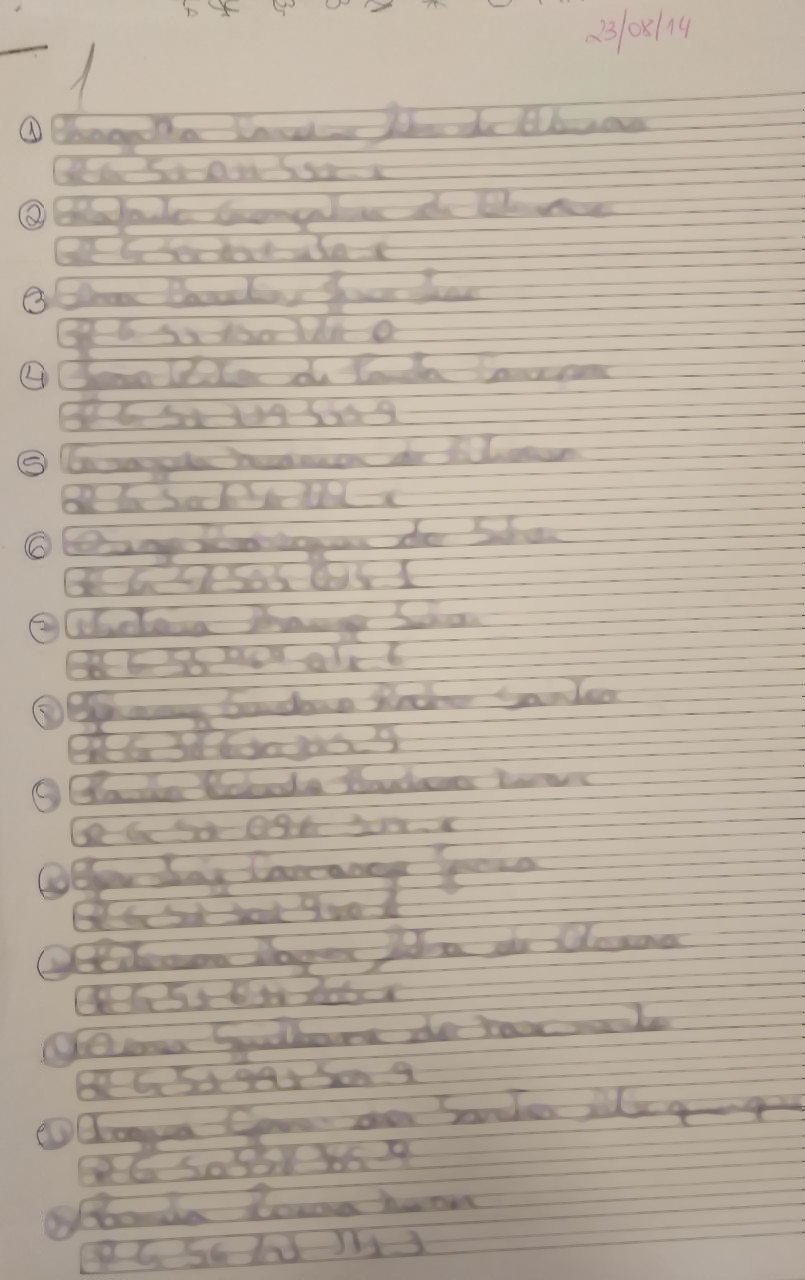
\includegraphics[width=1.0\linewidth]{../../imagens/blurred-Presenca-Oficina-2014-08-23.jpeg}
                \caption{Testemunhos de presen\c{c}a de estudantes do fundamental, em eventos do Programa WASH, coletados pela autora. O exemplo \'e de uma oficina em 23 de agosto de 2014. Nos prim\'ordios do Programa eram usados registros na forma de listas de presen\c{c}a em folhas de papel. A imagem foi desfocalizada para proteger a privacidade dos participantes. (fonte: acervo da autora)}
                \label{dec219c809788f521312f8d75d2f5591f069f132}
\end{minipage}%
\hspace{0.5cm}
\begin{minipage}[b]{0.4\linewidth}
        \centering
                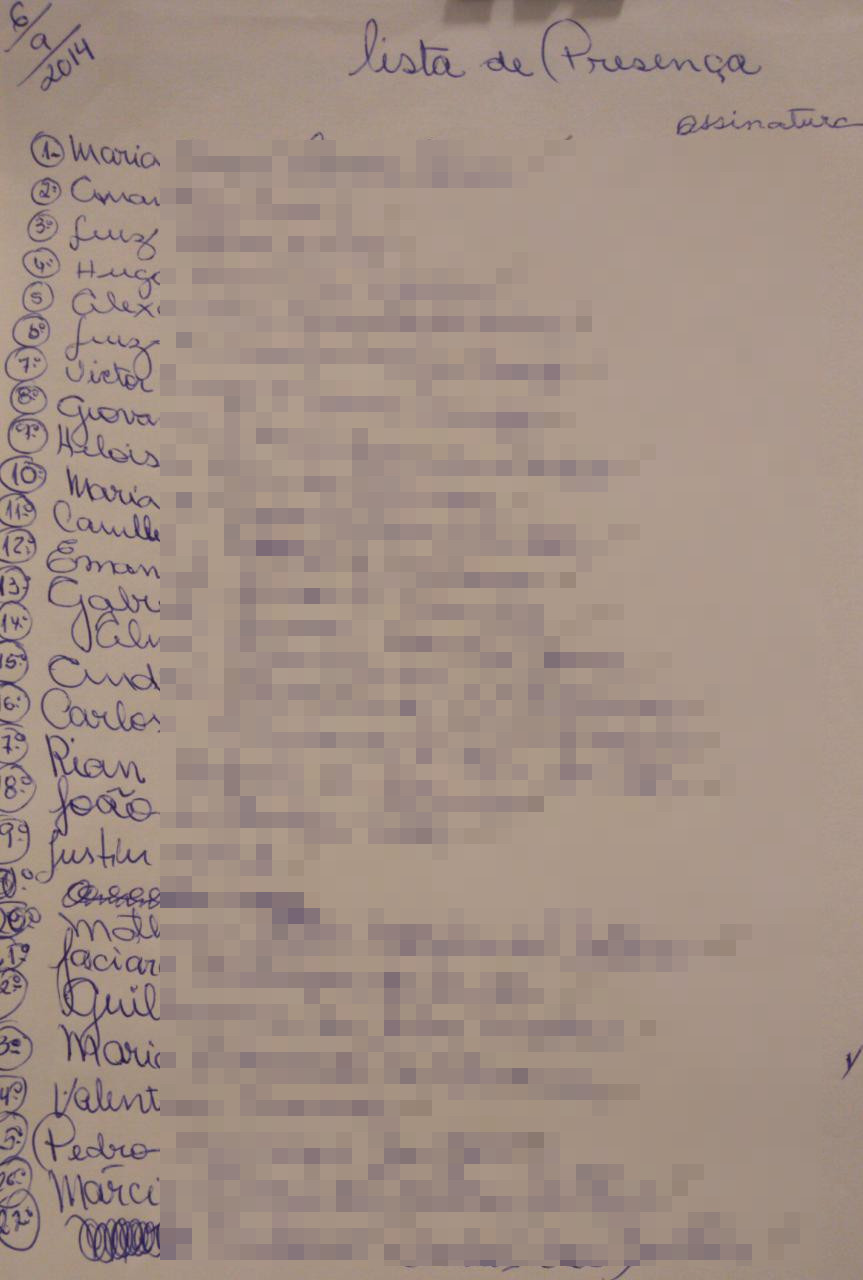
\includegraphics[width=1.0\linewidth]{../../imagens/blurred-Presenca-Oficina-2014-09-06.jpeg}
                \caption{Exemplo de lista de presen\c{c}a em papel, da oficina realizada em 6 de setembro de 2014. A imagem foi desfocalizada para proteger a privacidade dos participantes. Estes testemunhos eram coletados pela autora para permitir a posterior presta\c{c}\~ao de contas aos \'org\~aos de fomento. (fonte: acervo da autora)}
                \label{9a8c04c719fc4f9811165547ded35a00eb4fbeed}
\end{minipage}
\hspace{0.5cm}
\begin{minipage}[b]{0.4\linewidth}
        \centering
                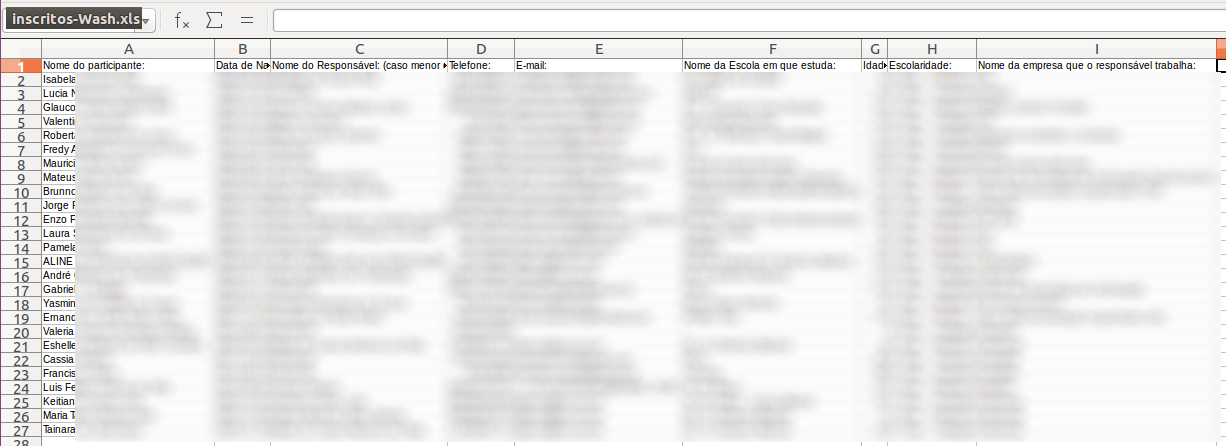
\includegraphics[width=1.0\linewidth]{../../imagens/blurred-planilha2.png}
                \caption{Planilhas eletr\^onicas tamb\'em foram empregadas para armazenar os registros de participa\c{c}\~oes, criando um protocadastro de participantes. A imagem foi desfocalizada intencionalmente para proteger a privacidade dos participantes. (fonte: acervo da autora)}
                \label{b43907f0fa6b6fb935e7384ab03b508859ff0609}
\end{minipage}%
\hspace{0.5cm}
\end{figure}



A Fig. 14 sumariza a evolu\c{c}\~ao do registro de presen\c{c}as, que se inicia com um manuscrito em folha de papel (2013), passando pelo registro em planilhas eletr\^onicas (2014) e chegando no uso pleno da plataforma Platu\'oxe (2022).














\captionsetup{format=plain}
\begin{figure}[htb]

	\begin{center}

		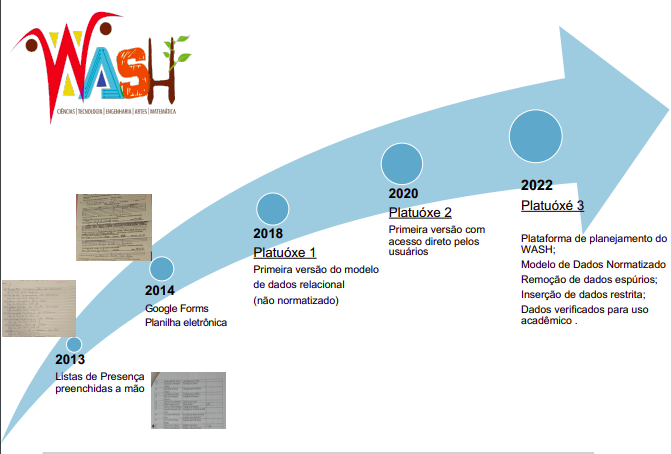
\includegraphics[max size={\textwidth}{\textheight}]{../../imagens/evolucao-da-documentacao.png}

	\end{center}

	\caption{\label{d237f9364cfe04892cbdffff7fea732012fa5804}Evolu\c{c}\~ao do m\'etodo de documenta\c{c}\~ao do WASH. (fonte: [[WASHCNPq (2022)]], com participa\c{c}\~ao da autora)}

\end{figure}

Esse cuidado em individualizar os participantes permitia, por exemplo, ter uma melhor no\c{c}\~ao do perfil et\'ario do p\'ublico atendido, bem como do interesse das pessoas em participar novamente das atividades, entre tantos outros indicadores que ficar\~ao mais claros no cap\'{\i}tulo de Resultados e An\'alise. Outro aspecto favor\'avel da individualiza\c{c}\~ao era uma melhor organiza\c{c}\~ao dos documentos do Programa, tais como autoriza\c{c}\~oes para a participa\c{c}\~ao de menores, consentimento de uso de imagem, identifica\c{c}\~ao de respons\'aveis para casos de emerg\^encia, entre outros.












A individualiza\c{c}\~ao das presen\c{c}as era obtida com o registro do nome do participante, o nome do respons\'avel e a data de nascimento. Dessa forma era diminu\'{\i}da a chance de confus\~ao entre hom\^onimos.












Assim, o desenvolvimento da \textquotedbl\{\}Platu\'oxe\textquotedbl\{\} nasceu com essa pr\'atica inicial de coleta e organiza\c{c}\~ao de testemunhos e controle de presen\c{c}a individualizado em oficinas, culminando com a disponibiliza\c{c}\~ao do sistema digital de registro.












A primeira vers\~ao do Platu\'oxe permitia registrar as oficinas realizadas, seus participantes e os testemunhos de realiza\c{c}\~ao, mas n\~ao dispunha de sistema de autentica\c{c}\~ao de usu\'ario. Por essa raz\~ao, requeria que os dados fossem registrados off-line. Mesmo com essa limita\c{c}\~ao, a primeira vers\~ao do software, que ficou pronta no in\'{\i}cio de 2019, passou a ser usada para gerar os indicadores do programa, de forma rastre\'avel, provendo meios confi\'aveis de prestar contas aos \'org\~aos de fomento e de controle, viabilizando melhores pr\'aticas de \textquotedbl\{\}compliance\textquotedbl\{\}.












A Platu\'oxe foi sendo evolu\'{\i}da paulatinamente a partir do teste constante de suas funcionalidades, atividade da qual participamos intensamente, juntamente com outros membros do Programa. A cada teste, eram identificados os problemas, com a subsequente propostas de alternativas, que eram implementadas pela equipe respons\'avel pela codifica\c{c}\~ao do Programa. Contribu\'{\i}ram substancialmente para essa fase de desenvolvimento as colegas Clotilde Maffra Diogo e Ana Carolina de Deus Soares.












Com a entrada do desenvolvedor Michel Alencar Morandi, a \textquotedbl\{\}Platu\'oxe\textquotedbl\{\} passou a dispor de um sistema de autentica\c{c}\~ao e todos os participantes do WASH puderam obter suas \textquotedbl\{\}contas de usu\'arios do sistema \textquotedbl\{\}, descentralizando a entrada de dados.












N\~ao obstante todos os esfor\c{c}os para criar uma ferramenta digital que facilitasse os registros de presen\c{c}a na plataforma, observaram-se muitas oficinas nas quais os registros fotogr\'aficos associados indicavam uma presen\c{c}a substancialmente maior do que estava registrado na lista de presen\c{c}a.













\noindent\begin{center}\mbox{\centering\fbox{\centering\par\parbox{0.7\linewidth}{\small\textit{Os dados da Platu\'oxe representam uma amostra do total de participantes no Programa.}\normalsize}}}\end{center}


Essa situa\c{c}\~ao ser\'a discutida no cap\'{\i}tulo de Resultados e An\'alise e est\'a, possivelmente, associada \`a falta de atribui\c{c}\~ao legal ao WASH para coletar dados de presen\c{c}a. Com essa limita\c{c}\~ao, o registro de presen\c{c}a \'e dependente da a\c{c}\~ao da entidade respons\'avel, introduzindo uma barreira para dinamizar a coleta de presen\c{c}as.












\subsection[Modelo relacional de dados do WASH]{Modelo relacional de dados do WASH}\label{Modelo relacional de dados do WASH}
Uma atividade fundamental conduzida pela equipe de codifica\c{c}\~ao da \textquotedbl\{\}Platu\'oxe\textquotedbl\{\} foi a modelagem de dados - MD, visando estabelecer as tabelas que seriam necess\'arias para representar os dados do WASH. Esta modelagem tinha como base as informa\c{c}\~oes fornecidas pelos (as) colaboradores do WASH envolvidos (as) com a opera\c{c}\~ao na ponta, entre eles (as), esta autora.












Como j\'a dito, uma das quest\~oes centrais no registro de dados do Programa WASH \'e saber quem s\~ao os(as) seus(suas) participantes. O Programa, por concep\c{c}\~ao, estimula participa\c{c}\~oes vol\'ateis, dado que as oficinas podem ser abertas e, como prev\^e o Documento de Refer\^encia do WASH, um novo participante consegue acompanhar uma oficina mesmo que n\~ao tenha vindo na anterior. Essa volatilidade \'e uma forma de estimular a inclus\~ao, uma vez que remove barreiras para a participa\c{c}\~ao. Ao mesmo tempo, cria desafios para como os dados ser\~ao representados.












No come\c{c}o da modelagem dos dados, havia uma d\'uvida sobre se dever\'{\i}amos criar uma tabela de cadastro para educandos(as), outra para os membros da equipe do WASH e mais outra para os (as) bolsistas (as) multiplicadores (as). A segunda op\c{c}\~ao seria criar uma tabela \'unica para todos (as) os (as) participantes, independentemente de seu papel no Programa. No caso da cria\c{c}\~ao de uma tabela \'unica, passam a ser necess\'arias tabela auxiliares, que, de forma coordenada, consigam representar os \textquotedbl\{\}tipos de papeis \textquotedbl\{\}  desempenhados pelos participantes no WASH.












A segunda op\c{c}\~ao (tabela \'unica de participantes com tabelas auxiliares) foi a escolhida porque j\'a se antecipava que o WASH seria um programa de longo prazo. Quando o sistema de registro come\c{c}ou a ser elaborado, o WASH j\'a tinha 6 anos e o crescimento anual indicava que haveria f\^olego para muitos anos de execu\c{c}\~ao. Assim, n\~ao fazia sentido separar os participantes em diversas tabelas, porque era razo\'avel esperar a mudan\c{c}a de pap\'eis dos participantes \`a medida, que os anos passavam, situa\c{c}\~ao que j\'a era observada em alguns casos, como explicamos a seguir.












De fato, observava-se que educandos do WASH, vinculados ao ensino fundamental, ao adentrar no ensino m\'edio, passavam a realizar sua inicia\c{c}\~ao cient\'{\i}fica, mudando de status para bolsistas multiplicadores do Programa. Bolsistas multiplicadores do ensino superior, por sua vez, ao se formarem em seus cursos, mudavam de status, assumindo pap\'eis no  \textquotedbl\{\}staff \textquotedbl\{\} do WASH; e, assim por diante. Muitos casos de transi\c{c}\~ao de pap\'eis (ou \textquotedbl\{\}status \textquotedbl\{\}) puderam ser constatados e a ideia de ter m\'ultiplas tabelas para participantes implicaria em um complicado sistema de transi\c{c}\~ao do registro de uma tabela para outra, quando o participante mudasse de papel. Outro motivo para usar uma tabela \'unica para representar participantes \'e que j\'a se observavam casos de pap\'eis simult\^aneos, a exemplo de multiplicadores que tamb\'em eram servidores p\'ublicos.












A tabela \'unica de participantes foi denominada \textquotedbl\{\}participantes2\textquotedbl\{\}, sendo parte da  \textquotedbl\{\}Platu\'oxe\textquotedbl\{\}. Esta tabela est\'a em uso at\'e os dias de hoje sendo complementada por tr\^es tabelas auxiliares, que tamb\'em s\~ao partes integrantes da \textquotedbl\{\}Platu\'oxe\textquotedbl\{\}. A primeira tabela auxiliar \'e \textquotedbl\{\}cargos \textquotedbl\{\}, que cont\'em os tipos de vincula\c{c}\~ao com o WASH. A segunda tabela auxiliar \'e \textquotedbl\{\}institui\c{c}\~oes \textquotedbl\{\}, que cont\'em as institui\c{c}\~oes a que um participante pode estar vinculado. Para relacionar o participante a um cargo e a uma institui\c{c}\~ao, foi criada a terceira tabela auxiliar denominada \textquotedbl\{\}afiliacoes \textquotedbl\{\}, que cont\'em a data de in\'{\i}cio e do fim daquela afialia\c{c}\~ao.












Este conjunto de 4 tabelas exemplifica a aplica\c{c}\~ao do m\'etodo de modelagem que foi empregado para representar os dados do WASH.












Come\c{c}aremos mostrando o conte\'udo (parcial) da tabela de \textquotedbl\{\}cargos\textquotedbl\{\}, representada na Tabela 6.
















\begin{table}[htb]
\tiny
\caption{\label{4d91d8ebc21ea7f9f54231ce125fae7980e789a3}Vis\~ao parcial da tabela cargos da base de dados do WASH. A tabela completa tem 42 linhas com registros de cargos.}

\centering
\begin{tabular}{|c|c|}
\hline
id\_chave\_cargo  &  nome\_cargo            \\
             9  &  Coordenador           \\
            10  &  Bolsista EXP A        \\
            11  &  Educando              \\
            13  &  Professor             \\
            15  &  Presidente            \\
            16  &  Diretor               \\
            17  &  Servidor              \\
            18  &  Coordenador Local     \\
            19  &  Coordenador Nacional  \\
            21  &  Deputado              \\
            22  &  Presidente            \\
            23  &  Multiplicador         \\
            25  &  Bolsista PCI   \\
            26  &  Bolsista ITI A \\
            27  &  Bolsista ITI B \\
            28  &  Reitor \\
            31  &  Secretaria \\
            38  &  Prefeito              \\
            39  &  Pesquisador           \\
            40  &  Secretaria Executiva             \\
            42  &  Estudante    \\
            43  &  Estagiario \\
            48  &  Bolsista EXP B \\
            49  &  Bolsista EXP C \\
            50  &  Bolsista ATP B \\
            51  &  Educando \\
            52  &  Voluntario \\
            54  &  Orientador            \\
            55  &  Bolsista DTI A \\
\hline
\end{tabular}
\end{table}


Na sequ\^encia, mostramos uma vis\~ao parcial da tabela \textquotedbl\{\}Instituicoes\textquotedbl\{\} (ver Tabela 7), que cont\'em todas as institui\c{c}\~oes atendidas pelo WASH. A tabela completa tem 150 linhas de registros de institui\c{c}\~oes, mas estamos mostrando apenas 38, por motivos de espa\c{c}o.
















\begin{table}[htb]
\tiny
\caption{\label{89e4a4c81cad3904f1348ca629486a33cc2c9bb6}Vis\~ao parcial da tabela instituicoes da base de dados do WASH. A tabela completa tem 150 linhas com registros, de institui\c{c}\~oes. Na presente reprodu\c{c}\~ao foram selecionados registros que mostram a pluralidade do atendimento do WASH, tendo sido retirados as repeti\c{c}\~oes de tipos de institui\c{c}\~oes por motivos de espa\c{c}o.}

\centering
\begin{tabular}{|c|c|}
\hline
id\_chave\_instituicao  &  nome\_instituicao \\
                  164  &  APAE  \\
                   68  &  Associa\c{c}\~ao Cultural Bola de Meia \\
                   74  &  Biblioteca Cidad\~a Paulo Freire  \\
                   52  &  Camara Federal \\
                   32  &  C\^amara Municipal de Campinas                                                      \\
                   25  &  Casa de Cultura Taina                                                             \\
                  168  &  CEI Vov\'o Maria                                                                    \\
                   23  &  Cemaden                                                                           \\
                  150  &  Centro de Forma\c{c}\~ao Popular Frei Betto                                             \\
                   19  &  Centro Paula Souza                                                                \\
                   22  &  Ci\^encia em Show                                                                   \\
                   57  &  CNPq                                                                              \\
                   91  &  Col\'egio Estadual Rio Branco                                                       \\
                   56  &  CPqD                                                                              \\
                    1  &  CTI Renato Archer                                                                 \\
                   70  &  E.E. Vitor Meireles                                                               \\
                   80  &  E.E. Expedito Camargo Freire                                                      \\
                  130  &  EMEF D\'ecio Moreira \\
                    5  &  Escola Dona Lindu \\
                  128  &  Escola Estadual MAJOR MIGUEL NAKED \\
                  111  &  ETEC Carapicu\'{\i}ba \\
                   47  &  Ex\'ercito Brasileiro \\
                  156  &  Faculdade Zumbi dos Palmares \\
                   53  &  FAPESP \\
                  119  &  Funda\c{c}\~ao Arauc\'aria \\
                   35  &  Governo do Estado de S\~ao Paulo \\
                  127  &  IFPR - Campus Pitanga \\
                   62  &  PUC de Campinas \\
                   21  &  Prefeitura de S\~ao Paulo           \\
                   48  &  Bolsista EXP \\
                   49  &  Secretaria de Cultura de Londrina \\
                   85  &  Secretaria de Educa\c{c}\~ao de Jacare\'{\i}/SP \\
                  169  &  SENAC Minas  \\
                   38  &  Sindicato dos Metal\'urgicos do ABC \\
                   16  &  Unicamp \\
                   75  &  UNIFESP  \\
                    9  &  USP \\
                  181  &  UTFPR \\
\hline
\end{tabular}
\end{table}


Para dar prosseguimento \`a exemplifica\c{c}\~ao, agora isolaremos um participante do Programa, separando seu registro do resto da tabela \textquotedbl\{\}participantes2\textquotedbl\{\} (ver Tabela 8). Note que a tabela original (participantes2)  tem 3312 registros, (linhas) mas decidimos usar como exemplo um \'unico participante, resultando em apenas uma linha na Tabela 8. Substitu\'{\i}mos o nome do participante para proteger sua privacidade, substituindo-o por um nome fict\'{\i}cio (\textquotedbl\{\}Maria Pereira \textquotedbl\{\}).
















\begin{table}[htb]
\tiny
\caption{\label{96081f1bc28f7c738012f4beb3ef867b6b67107f}Exemplo de linha da tabela participantes2, selecionada para que se possa entender como o registro dos pap\'eis desempenhados por cada participante \'e feito no \^ambito do WASH. A tabela participantes2 tem 3312 registros de participantes.}

\centering
\begin{tabular}{|c|c|c|}
\hline
id\_chave\_participante  &  nome\_participante             &  data\_nascimento  \\
                     2  &  Maria Pereira  &  1994-06-15 \\
\hline
\end{tabular}
\end{table}


\'E importante observar, na \'ultima coluna da Tabela 8 que, por escolha da \'area de TI do WASH, todas as datas no \^ambito dos registros do Programa s\~ao invertidas, sempre come\c{c}ando pelo ano, passando pelo m\^es e terminando no dia. Isto \'e feito assim para garantir que a ordena\c{c}\~ao dos registros por data seja facilitada.












Agora, vamos extrair da tabela \textquotedbl\{\}afiliacoes\textquotedbl\{\}, (ver Tabela 9) todos os registros cujo identificador de participante seja \textquotedbl\{\}2 \textquotedbl\{\}, como consta no excerto da tabela participantes2 mostrado na Tabela 8.
















\begin{table}[htb]
\tiny
\caption{\label{e6120545268b93238330297571c4756e7c97df1a}Subconjunto de registro da tabela afiliacoes, onde foram selecionados apenas os dados do participante que tem identificador 2 na tabela participantes2.}

\centering
\begin{tabular}{|c|c|c|c|c|c|}
\hline
id\_participante  &  id\_instituicao  &  id\_cargo  &  nome\_documento  &  inicio      &  fim \\
              2  &              62  &        42  &  RA12345679      &  2012-02-01  &  2015-01-31  \\
              2  &              57  &        48  &  111111/2018-9   &  2018-08-01  &  2019-07-31  \\
              2  &              57  &        48  &  222222/2019-6   &  2019-08-01  &  2019-12-31  \\
              2  &              57  &        48  &  333333/2019-2   &  2020-08-01  &  2021-12-31  \\
              2  &              57  &        26  &  444444/2016-1   &  2016-08-02  &  2017-07-31  \\
              2  &              62  &        52  &  n\~ao consta      &  2015-08-01  &  2016-08-01 \\
\hline
\end{tabular}
\end{table}


O excerto da tabela \textquotedbl\{\}afiliacoes\textquotedbl\{\} mostrado na tabela 9 indica que a participante identificada pelo n\'umero 2 (Maria Pereira)  teve duas afilia\c{c}\~oes durante o per\'{\i}odo em que esteve vinculada ao WASH: \`a universidade PUC de Campinas, que \'e identificada pelo n\'umero 62 e ao CNPq, que \'e identificado pelo n\'umero 57 (se tiver d\'uvida, veja o identificador dessas institui\c{c}\~oes na Tabela 7).












Al\'em disso, essa mesma participante identificada pelo n\'umero 2 desempenhou 4 pap\'eis no WASH (ver Tabela 6): estudante, identificado pelo n\'umero 42, Bolsista EXP B, identificado pelo n\'umero 48 e Bolsista ITI A, identificado pelo n\'umero 26.












A tabela \textquotedbl\{\}afiliacoes\textquotedbl\{\} tamb\'em permite conhecer o documento que formaliza a vincula\c{c}\~ao com o Programa WASH, pelo campo nome\_documento (ver Tabela 9). Os campos \textquotedbl\{\}inicio \textquotedbl\{\} e \textquotedbl\{\}fim \textquotedbl\{\} permitem conhecer o per\'{\i}odo em que uma determinada afilia\c{c}\~ao estava v\'alida.












O exemplo mostrado at\'e agora permite compreender o m\'etodo baseado em bancos de dados relacionais de uma forma pr\'atica.












O sistema de armazenamento de dados do WASH \'e integralmente baseado nessa l\'ogica de m\'ultiplas tabelas, que se relacionam por meio de identificadores num\'ericos. Esse m\'etodo \'e bastante robusto e reduz sobremaneira a ocorr\^encia de dados esp\'urios, muito embora ainda exista a possibilidade de algum erro estar presente, porque a integridade da base de dado \'e dependente da qualidade do preenchimento de dados. Isso quer dizer que, para garantir a qualidade de dados, \'e preciso uma capacita\c{c}\~ao constante dos colaboradores.












A maior robustez do m\'etodo relacional vem justamente do fato de que a informa\c{c}\~ao est\'a segregada, de forma que em cada tabela exista apenas um registro para cada fato representado. Em outras palavras: note que na tabela \textquotedbl\{\}participantes2\textquotedbl\{\} (ver Tabela 2) existir\'a apenas 1 registro para o participante que \'e identificado pelo n\'umero 2 (Maria Pereira), ao passo que na tabela \textquotedbl\{\}cargos \textquotedbl\{\} (ver Tabela 6) haver\'a apenas um registro identificado pelo n\'umero 48 (Bolsista EXP B), da mesma forma que na tabela \textquotedbl\{\}instituicoes \textquotedbl\{\} (ver Tabela 7) haver\'a apenas um registro identificado pelo n\'umero 57 (CNPq).












Vimos que o participante identificado pelo n\'umero \textquotedbl\{\}2 \textquotedbl\{\} teve  pelo menos 6 diferentes tipos de v\'{\i}nculos com o WASH, em momentos diferentes de sua atua\c{c}\~ao, mas n\~ao foi preciso criar 6 registros na tabela \textquotedbl\{\}participantes2\textquotedbl\{\}. Se o WASH usasse planilhas eletr\^onicas para guardar seus dados seria necess\'ario repetir 6 vezes todas as informa\c{c}\~oes sobre o participante, criando a oportunidade para falta de uniformiza\c{c}\~ao de dados e, portanto, perda de confiabilidade nos mesmos.












Para representar todos os seus dados de forma flex\'{\i}vel e adapt\'avel \`as suas diversas parcerias, o sistema de armazenamento de dados do WASH precisou criar 54 tabelas, como mostrado na Tabela 10.
















\begin{table}[htb]
\tiny
\caption{\label{5b2e4ba8f3836249e7dd88b37344da7bfa3669c5}O banco de dados relacional da Platu\'oxe \'e constitu\'{i}do por 54 tabelas}

\centering
\begin{tabular}{|c|c|}
\hline
afiliacoes                     &   local\_eventos \\
 atividades                     &   local\_part \\
 atividades\_eventos             &   modelo\_atividades\_eventos \\
 atividades\_fotos               &   modelo\_documentos\_eventos \\
 avaliacao\_bolsista             &   modelo\_eventos \\
 bolsa\_cnpq                     &   modelo\_tematicas\_eventos \\
 cargos                         &   parametros \\
 comentario\_evento              &   part\_eventos \\
 compartilhados                 &   participantes2 \\
 documentos                     &   processo\_cnpq \\
 documentos\_equipes             &   processo\_ivan\_valente \\
 documentos\_eventos             &   processo\_wash\_ABC \\
 documentos\_instituicoes        &   processo\_wash\_cury \\
 documentos\_participantes       &   processo\_wash\_regioes \\
 estimativa                     &   relacao\_grupo\_modelo \\
 eventos                        &   responsaveis\_eventos \\
 fontes                         &   status \\
 fontes\_eventos                 &   status\_doc \\
 formacao                       &   tematicas \\
 fotos                          &   tematicas\_eventos \\
 grupo\_evento                   &   tipo\_documento \\
 grupo\_modelo                   &   tipos\_encerramento \\
 grupo\_participante             &   trash \\
 grupos                         &   trash\_fontes \\
 inst\_eventos                   &   trash\_fotos \\
 instituicoes                   &   vincula\_instituicao\_instituicao \\
 locais                         &   vincula\_local\_instituicao \\
\hline
\end{tabular}
\end{table}


N\~ao aprofundaremos mais na descri\c{c}\~ao da modelagem de dados do Platu\'oxe por raz\~oes de espa\c{c}o, mas acreditamos que as informa\c{c}\~oes at\'e agora compartilhadas permitem ao leitor compreender o m\'etodo de registro de dados utilizado nesta disserta\c{c}\~ao.












\subsection[Consulta \`a base de dados atrav\'es da Linguagem SQL]{Consulta \`a base de dados atrav\'es da Linguagem SQL}\label{Consulta \`a base de dados atrav\'es da Linguagem SQL}
Vimos no cap\'{\i}tulo de Fundamenta\c{c}\~ao Te\'orica um r\'apida descri\c{c}\~ao dos princ\'{\i}pios da Linguagem SQL.1












Essa linguagem foi extensamente utilizada como m\'etodo para obter os indicadores deste Projeto. Para isso, foi aplicada \`a base de dados relacional da plataforma Platu\'oxe descrita na se\c{c}\~ao anterior.












As consultas SQL foram elaboradas pela equipe de TI, com base nas especifica\c{c}\~oes dos indicadores de interesse para esta autora. Em algumas situa\c{c}\~oes, os resultados dessas consultas puderam ser verificados pelo emprego de uma planilha eletr\^onica, elaborada pela autora.












\subsection[M\'etodo de determina\c{c}\~ao do sexo dos participantes]{M\'etodo de determina\c{c}\~ao do sexo dos participantes}\label{M\'etodo de determina\c{c}\~ao do sexo dos participantes}
A maior preval\^encia de participa\c{c}\~ao masculina em atividades STEAM, em detrimento da feminina, \'e um fen\^omeno que, infelizmente, se reproduz mundialmente (Kijima et al., 2021). Cabe ao WASH verificar, da melhor forma poss\'{\i}vel, se essa situa\c{c}\~ao injusta est\'a sendo reproduzida dentro do pr\'oprio Programa, com vistas a promover interven\c{c}\~oes que possam mitig\'a-la.












Com a finalidade de verificar essa situa\c{c}\~ao, decidimos incluir, entre os indicadores do Programa, o percentual de mulheres e homens participantes. Isso exigiu um esfor\c{c}o de cria\c{c}\~ao de um m\'etodo especial, uma vez, que antes de 2019 o WASH n\~ao armazenava dados de sexo ou g\^enero.












\'E poss\'{\i}vel identificar v\'arios est\'agios, ao longo da exist\^encia do WASH, referentes \`a forma de armazenar dados (ver Fig. 14). Foi comentando na se\c{c}\~ao anterior que logo no in\'{\i}cio do Programa, por exemplo, os dados de participantes eram coletados por meio de listas de presen\c{c}a em papel (ver Figs. 11, 12 e 13). Estas listas registravam apenas o nome dos participantes e a data do evento, sem registro de sexo. Posteriormente, novos dados foram sendo coletados, como o ano do nascimento da crian\c{c}a, seu Registro Geral (RG) ou do respons\'avel, mas ainda sem registrar o sexo.












1Esse crescimento gradativo na quantidade de dados coletados revela, por parte da Coordena\c{c}\~ao do WASH, um cuidado de armazenar exclusivamente dados que estavam vinculados aos objetivos do Programa. Essa vis\~ao decorre do Programa n\~ao ter um mandato espec\'{\i}fico (atribui\c{c}\~ao legal) para registro de dados cadastrais mais detalhados. Na falta desse mandato, o registro sem prop\'osito desses dados pode ser considerado prejudicial \`a privacidade dos participantes, requerendo custosas medidas de prote\c{c}\~ao de dados adicionais.












Assim, \'e poss\'{\i}vel compreender porque a coleta de dados sempre foi mantida no limite dos prop\'ositos do projeto, a saber: contabilizar o n\'umero de participantes, evitar a contagem duplicada de participantes, identificar os respons\'aveis para o caso de emerg\^encias, registrar autoriza\c{c}\~oes de uso de imagens, e assim por diante.












Em outras palavras, por falta de conex\~ao com os objetivos iniciais do Programa, n\~ao havia armazenagem de dados de sexo de seus participantes.












Com o passar dos anos, percebeu-se que o projeto j\'a contava com milhares de cadastros incompletos, comprometendo a avalia\c{c}\~ao equ\^anime do Programa mencionada no come\c{c}o desta se\c{c}\~ao.












Para vencer essa defici\^encia de cadastro, decidiu-se por criar um m\'etodo em que os indicadores de sexo do WASH pudessem ser constru\'{\i}dos a partir de uma avalia\c{c}\~ao a posteriori (em rela\c{c}\~ao ao momento do cadastro) dos primeiros nomes dos participantes. Esse m\'etodo pode ser sumarizado como:













\noindent\begin{center}\mbox{\centering\fbox{\centering\par\parbox{0.7\linewidth}{\small\textit{O m\'etodo consiste em verificar se o primeiro nome de cada participante est\'a numa lista extensiva de nomes \textquotedbl\{\}considerados masculinos\textquotedbl\{\}, situa\c{c}\~ao em que, de forma anonimizada, um contador de participantes masculinos \'e incrementado. Caso o primeiro nome do participante esteja numa lista de nomes \textquotedbl\{\}considerados femininos\textquotedbl\{\}, o contador de participantes femininos \'e incrementado. Quando o nome n\~ao est\'a em nenhuma das listas ou quando \'e um nome com sexo indefinido, o contador de \textquotedbl\{\}sexo desconhecido\textquotedbl\{\} \'e incrementado.}\normalsize}}}\end{center}


A rigor, do ponto de vista do WASH, n\~ao h\'a interesse em rotular peremptoriamente as pessoas com base no sexo identificado por esse m\'etodo. Por essa raz\~ao, o dado de sexo gerado n\~ao \'e vinculado ao cadastro do participante, ficando armazenado num contador anonimizado.












Dito isso, o fato \'e que o primeiro nome do participante n\~ao permite avaliar a identidade de g\^enero. Assim, a postura limita a coleta de dados gerando uma reconhecida defici\^encia de registro associada \`a falta de coleta de dados autodeclarat\'orios de g\^enero antes de 2019.












Mesmo reconhecida esta defici\^encia, os n\'umeros encontrados (ver Resultados e An\'alise) indicam que a estimativa produzida pelo m\'etodo \'e suficiente para suportar a avalia\c{c}\~ao das hip\'oteses desse trabalho.












\chapter[RESULTADOS E AN\'ALISES]{RESULTADOS E AN\'ALISES}\label{RESULTADOS E AN\'ALISES}
Alcan\c{c}amos o final dos caminhos percorridos (m\'etodos) descritos no cap\'{\i}tulo anterior, criando as condi\c{c}\~oes para que os resultados obtidos sejam apresentados.












Os resultados obtidos ser\~ao descritos e, concomitantemente, analisados para que a validade das hip\'oteses levantadas possa ser verificada.












Os resultados est\~ao organizados, inicialmente, em duas se\c{c}\~oes separadas, relacionadas aos eixos da da presente pesquisa:













\begin{alineas}
\item hist\'oria (eixo 1)
\item indicadores (eixo 2); e
\end{alineas}

Ser\'a apresentada uma terceira se\c{c}\~ao contendo uma s\'{\i}ntese que integrar\'a os achados dos dois eixos indicados acima. Esta terceira se\c{c}\~ao analisar\'a cada hip\'otese separadamente.












\section[Narrativas contru\'{\i}das a partir do m\'etodo historiogr\'afico (eixo 1)]{Narrativas contru\'{\i}das a partir do m\'etodo historiogr\'afico (eixo 1)}\label{Narrativas contru\'{\i}das a partir do m\'etodo historiogr\'afico (eixo 1)}
Aqui, s\~ao apresentadas as narrativas constru\'{\i}das a partir da aplica\c{c}\~ao do m\'etodo historiogr\'afico, descrito em Materiais e M\'etodos.












O m\'etodo utilizado se baseia na an\'alise do acervo de documentos oficiais (portarias, planos de trabalho, termos de outorga, boletins, legisla\c{c}\~ao, entre outros), registros pessoais da autora (fotografias, v\'{\i}deos, di\'arios, entre outros) e literatura (artigos, not\'{\i}cias, entre outros), complementados pelas mem\'orias narradas pelos part\'{\i}cipes do percurso hist\'orico em estudo. Estas mem\'orias foram colhidas pela autora por meio de entrevistas.












Como j\'a indicado no Cap\'{\i}tulo de Materiais e M\'etodos, no texto final da narrativa hist\'orica, buscamos intercalar conhecimentos obtidos do acervo com trechos selecionados das entrevistas citadas, complementando o olhar objetivo da autora com a subjetividade dos atores entrevistados.












\subsection[O GESAC e sua contribui\c{c}\~ao para  a cultura  digital  no pa\'{\i}s]{O GESAC e sua contribui\c{c}\~ao para  a cultura  digital  no pa\'{\i}s}\label{O GESAC e sua contribui\c{c}\~ao para  a cultura  digital  no pa\'{\i}s}
Vimos na Introdu\c{c}\~ao que os benef\'{\i}cios e conforto trazidos para os dias de hoje por esse admir\'avel mundo novo digital s\~ao resultados de a\c{c}\~oes e iniciativas da ci\^encia e da tecnologia, que foram deflagradas l\'a nos anos 50, impulsionadas ao longo das d\'ecadas seguintes, mas cuja populariza\c{c}\~ao e dissemina\c{c}\~ao se intensificaram nos anos 90.












Os anos 90 s\~ao considerados como os anos dourados para que cheg\'assemos \`a atual configura\c{c}\~ao de planeta tecnol\'ogico e informatizado, que vivencia a Sociedade da Informa\c{c}\~ao em suas v\'arias dimens\~oes. Esta afirma\c{c}\~ao se sustenta na consolida\c{c}\~ao das cadeias produtivas, que permitiram reduzir o custo dos equipamentos digitais e sua consequente difus\~ao  (CIPOLI, 2012), preparando o mundo para o crescimento do acesso \`as redes digitais observado na d\'ecada seguinte, como exemplificado na Fig. 1, em que \'e mostrado o crescimento do acesso \`a internet no Brasil.












Dentre os  in\'umeros feitos dessa \'epoca, basta lembrarmos o surgimento da Internet, a populariza\c{c}\~ao do computador pessoal e a chegada dos dispositivos m\'oveis (celulares).












Na esfera governamental, o Brasil assistiu, a partir de 2003, bem no in\'{\i}cio do Governo Lula, a implanta\c{c}\~ao do Governo Eletr\^onico e Servi\c{c}o de Atendimento ao Cidad\~ao- GESAC.












Mas, o Programa tinha sido institu\'{\i}do oficialmente um ano antes, pelo Minist\'erio das Comunica\c{c}\~oes do Governo FHC, por meio  da Portaria nº. 256, de 13 de mar\c{c}o de 2002 (BRASIL, 2004b), cujo  objetivo era disseminar meios que permitissem a universaliza\c{c}\~ao do acesso \`as informa\c{c}\~oes e servi\c{c}os do governo, por meio eletr\^onico no territ\'orio nacional, a toda popula\c{c}\~ao brasileira (BRASIL, 2002).












A licita\c{c}\~ao para a contrata\c{c}\~ao de uma empresa para implanta\c{c}\~ao do Programa GESAC foi realizada durante o governo FHC, no ano de 2002. Na \'epoca, foram alocados para o Programa GESAC recursos da ordem de 86 milh\~oes de reais para serem investidos ao longo de 18 meses.












Ant\^onio Albuquerque, entrevistado pela autora e primeiro Diretor Nacional do GESAC, traz uma vis\~ao esclarecedora do que previa a proposta de 2002:













\noindent\begin{center}\mbox{\centering\fbox{\centering\par\parbox{0.7\linewidth}{\small\textit{\textquotedbl\{\}A proposta do GESAC, originalmente estabelecida no Governo FHC, tinha algumas defici\^encias. Por exemplo, o GESAC original previa apenas instala\c{c}\~ao de infraestrutura para permitir o acesso a sites do governo, sem nenhuma apropria\c{c}\~ao tecnol\'ogica por parte das comunidades. Outra defici\^encia era escolha dos locais de instala\c{c}\~ao dos pontos de presen\c{c}a, que seria feita pela empresa contratada, sem uma articula\c{c}\~ao para identificar onde realmente estavam as pessoas mais necessitadas. Outro problema era a t\'{\i}mida abrang\^encia prevista para o programa, que com poucos milhares de computadores planejados, n\~ao contemplava o desafio de levar inclus\~ao digital para um pa\'{\i}s continental como o Brasil. Em suma, o Programa GESAC, como estava especificado no processo licitat\'orio de 2002, estava muito aqu\'em do que deveria ser um verdadeiro Programa de inclus\~ao digital.\textquotedbl\{\} (fonte: entrevista com Ant\^onio Albuquerque, Diretor Nacional do Programa GESAC em 2003)}\normalsize}}}\end{center}


O entendimento manifesto pela Coordena\c{c}\~ao do Relacionamento com as Comunidades do Programa GESAC, Toni Klaus, tamb\'em entrevistado por esta autora, corrobora com a vis\~ao trazida por Ant\^onio Albuquerque, acrescentando que a proposta de 2002, embora licitada, nunca fora colocada em pr\'atica:













\noindent\begin{center}\mbox{\centering\fbox{\centering\par\parbox{0.7\linewidth}{\small\textit{\textquotedbl\{\}Para se falar do GESAC , eu entendo que temos que situ\'a-lo no tempo. O Governo Lula estava come\c{c}ando em 2003 e a internet estava em amplo processo de populariza\c{c}\~ao no Brasil e no mundo, desde 1996. O GESAC foi uma iniciativa do governo FHC, que nunca tinha sido executada. A iniciativa original previa 1200 Pontos de Presen\c{c}a, para serem disponibilizados em lugares p\'ublicos, tais como quiosques para acesso \`a internet pela popula\c{c}\~ao, em postos dos correios e outras localiza\c{c}\~oes semelhantes. Mas, esse contrato nunca foi executado no \^ambito do governo FHC.\textquotedbl\{\} (fonte: entrevista com Toni Klaus Bochat,Programa GESAC entre 2003 e 2005)}\normalsize}}}\end{center}


O implementador do GESAC, Angel Luis, sintetiza as duas vis\~oes sobre a proposta de 2002 com a met\'afora de \textquotedbl\{\}Guich\^e Eletr\^onico\textquotedbl\{\}:













\noindent\begin{center}\mbox{\centering\fbox{\centering\par\parbox{0.7\linewidth}{\small\textit{\textquotedbl\{\}O Programa tinha a finalidade inicial (em 2002) de ser o \textquotedbl\{\}guich\^e eletr\^onico\textquotedbl\{\} do governo federal.\textquotedbl\{\} (fonte: entrevista com o implementador do GESAC, Angel Luis)}\normalsize}}}\end{center}


Foi durante o ano de 2003, no primeiro Governo Lula, que de fato iniciou-se o funcionamento do  GESAC. Os gestores que assumiram a responsabilidade pelo Programa usaram o primeiro semestre de 2003 para que se fizessem as adequa\c{c}\~oes administrativas e t\'ecnicas necess\'arias para transform\'a-lo em um amplo processo de inclus\~ao digital. Essas adequa\c{c}\~oes foram resultado de mudan\c{c}as conceituais no Programa GESAC com altera\c{c}\~oes de seus princ\'{\i}pios, colocando seus benefici\'arios como protagonistas do processo de inclus\~ao digital.












No segundo semestre de 2003, o Programa GESAC foi efetivamente implantado com os Pontos de Presen\c{c}a (PPs), espa\c{c}o com  computadores conectados \`a internet, via sat\'elite. \`A \'epoca, cada PP deveria ter, no m\'{\i}nimo, entre cinco e quinze computadores, podendo ser utilizados gratuitamente por cada comunidade local.












Com a readequa\c{c}\~ao do Programa GESAC, foi criado o Departamento de Inclus\~ao Digital - DESID, no Minist\'erio das Comunica\c{c}\~oes, sendo nomeado como diretor, Ant\^onio Bezerra de Albuquerque, que conduziu a implanta\c{c}\~ao e gest\~ao do GESAC. Posteriormente esse executivo, veio a contribuir tamb\'em com o Programa WASH.













\noindent\begin{center}\mbox{\centering\fbox{\centering\par\parbox{0.7\linewidth}{\small\textit{\textquotedbl\{\}No inicio de 2003, o engenheiro Ant\^onio Albuquerque, funcion\'ario de carreira do CPqD da Telebr\'as da cidade de Campinas, \'e designado  assessor especial do Ministro das Comunica\c{c}\~oes. Uma  de suas tarefas foi analisar o contrato do GESAC e, se necess\'ario, fazer as adequa\c{c}\~oes contratuais, atendendo \`as novas diretrizes de inclus\~ao digital do governo federal. Foi adotado o uso do software livre e disponibilizado um data-center com um conjunto de ferramentas destinadas aos usu\'arios  para a produ\c{c}\~ao de conte\'udos e suporte operacional.\textquotedbl\{\} (fonte: entrevista com Toni Klaus Bochat, Programa GESAC entre 2003 e 2009)}\normalsize}}}\end{center}


O primeiro Ponto de Presen\c{c}a - PP foi  instalado na  Escola Estadual Belmiro Soares, na cidade de Paranaguaiara, em  Goi\'as.












As diretrizes de pol\'{\i}tica p\'ublica de inclus\~ao digital que o GESAC procurou atender, a partir de 2003 foram:













\begin{alineas}
\item oferecer acesso aos servi\c{c}os de governo eletr\^onico (e-gov);
\item acesso \`a internet deveria ser irrestrito;
\item oferecer conex\~ao de banda larga, via sat\'elite (ver antena GESAC na Fig. 15), para atender \`as comunidades sem infraestrutura,  em localidades distantes, que n\~ao poderiam ter acesso a esse servi\c{c}o;
\item implantar uso e gest\~ao comunit\'aria dos equipamentos, possibilitando a apropria\c{c}\~ao coletiva  da tecnologia,  desenvolvimento local atrav\'es de apoio \`a produ\c{c}\~ao econ\^omica, educativa e cultural da comunidade;
\item oferecer uma cesta de servi\c{c}os on-line de apoio ao usu\'ario para o processo de inclus\~ao digital, disponibilizando correio eletr\^onico (e-mail),  jornal mural (Teia), sistema de compartilhamento de informa\c{c}\~oes ( RAU-TU) e hospedagem de s\'{\i}tios eletr\^onicos produzidos pela comunidade (Pousada). Todos os servi\c{c}os  foram oferecidos em software livre, conforme as diretrizes do governo da \'epoca;
\item cria\c{c}\~ao do portal IDBRASIL para estabelecer um canal de comunica\c{c}\~ao entre o MC e as comunidades e entre as pr\'oprias comunidades. Esse portal dava acesso aos servi\c{c}os do programa e ao compartilhamento  de informa\c{c}\~oes  entre as comunidades usu\'arias;
\item promover a apropria\c{c}\~ao das TICS  para as comunidades usu\'arias, por meio de  capacita\c{c}\~oes e oficinas de forma\c{c}\~ao de multiplicadores.
\item Disponibiliza\c{c}\~ao de uma plataforma multisservi\c{c}os com voz sobre ip, servi\c{c}o 0800, 700 mil caixas postais de e-mail, espa\c{c}os para produ\c{c}\~ao de “homepages”, canal de IP-TV, multicasting, oficinas de cultura digital, encontros de forma\c{c}\~ao e outros;
\end{alineas}



\captionsetup{format=plain}
\begin{figure}[htb]

	\begin{center}

		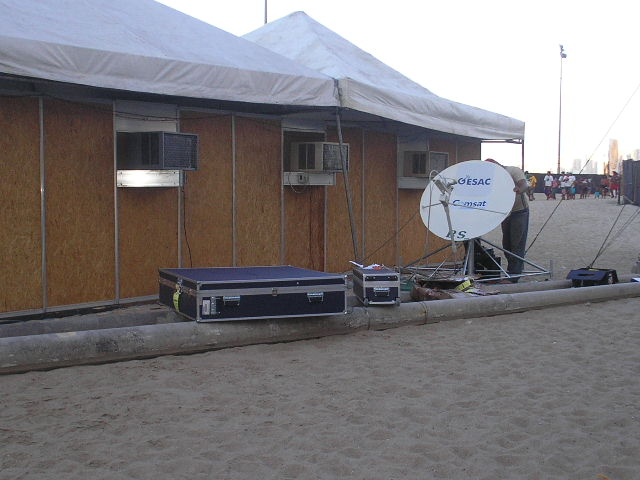
\includegraphics[max size={\textwidth}{\textheight}]{../../imagens/antenagesac.jpg}

	\end{center}

	\caption{\label{a3225c07ca3bc896130a8519e74f575fb919fefd}Antena Gesac, instalada nos jogos ind\'{i}genas.}

\end{figure}

Tinha-se a compreens\~ao que somente a disponibiliza\c{c}\~ao de equipamentos tecnol\'ogicos n\~ao era suficiente, mas  era imprescind\'{\i}vel que o Programa contribu\'{\i}sse para a forma\c{c}\~ao dos usu\'arios no uso das tecnologias de informa\c{c}\~ao e comunica\c{c}\~ao. Em 2004, passou-se a oferecer oficinas de capacita\c{c}\~ao,em campo, \`as comunidades atrav\'es de profissionais denominados como implementadores sociais, pessoas com habilidades t\'ecnicas,  que realizavam o trabalho de forma\c{c}\~ao  e apropria\c{c}\~ao das TICS pelas comunidades.












O grupo de implementadores(as) sociais passou por um processo de sele\c{c}\~ao e forma\c{c}\~ao sobre o Programa. A escolha buscava identificar habilidades t\'ecnicas e sociais, com vistas \`a atua\c{c}\~ao em diversas comunidades. Para garantir pluralidade, os implementadores (as) eram oriundos(as) de todas as regi\~oes do Brasil. A forma\c{c}\~ao destes (as) implementadores (as) buscava  permitir que eles (elas) aprendessem, dominassem, compartilhassem  e disseminassem a utiliza\c{c}\~ao dos servi\c{c}os oferecidos pelo GESAC, assim como a ado\c{c}\~ao e o uso de software livre. Essas pessoas visitavam as comunidades de Norte a Sul do pa\'{\i}s, preparando e realizando oficinas, e fazendo a migra\c{c}\~ao para o uso do software livre. O Programa GESAC seguia as Diretrizes, Objetivos e A\c{c}\~oes priorit\'arias para implementar o uso do Software Livre, conforme estabelecido no Planejamento Estrat\'egico 2003-2004, organizado pela  Casa Civil, Presid\^encia Rep\'ublica, em que essa autora fez parte do Comit\^e T\'ecnico de implementa\c{c}\~ao do Software Livre.












Entre as atividades que deveriam realizar estavam:













\begin{alineas}
\item instala\c{c}\~ao de laborat\'orios (as atividades inclu\'{\i}am, por exemplo, a capacita\c{c}\~ao em cabeamento de rede, migra\c{c}\~ao de softwares propriet\'arios para software livre, dentre outras atividades t\'ecnicas)
\item promo\c{c}\~ao de encontros locais e estaduais do programa,
\item colabora\c{c}\~ao para que os  Pontos de Presen\c{c}a organizassem o seu comit\^e de gestor,
\item resolu\c{c}\~ao ou encaminhamento de poss\'{\i}veis quest\~oes t\'ecnicas.
\end{alineas}

A cada implementador (a) era disponibilizado um equipamento GPS, celular, notebook, projetor multim\'{\i}dia e kit de ferramentas. O papel mais vis\'{\i}vel das pessoas que atuavam na condi\c{c}\~ao de implementadores (as) era o de oferecer as oficinas de cultura digital, bem como colaborar para que a as pessoas inseridas em suas comunidades tivessem acesso e pudessem se apropriar das tecnologias da informa\c{c}\~ao e comunica\c{c}\~ao que estavam sendo disponibilizadas.













\noindent\begin{center}\mbox{\centering\fbox{\centering\par\parbox{0.7\linewidth}{\small\textit{\textquotedbl\{\}Os implementadores sociais trabalhavam localmente nos pontos implantados, principalmente com os administradores desses pontos. A ideia era multiplicar os conhecimentos do mundo digital para os usu\'arios locais. Eram feitas oficinas sobre os servi\c{c}os disponibilizados pelo GESAC, mas tamb\'em sobre Software Livre em geral (ver Figs. 17 e 18)). O uso de software livre era uma pol\'{\i}tica p\'ublica do governo federal e, portanto, todos os computadores do programa tinham uma distribui\c{c}\~ao em software livre. Os servi\c{c}os disponibilizados tamb\'em eram em software livre.\textquotedbl\{\} (fonte: entrevista com Toni Klaus Bochat, do Programa GESAC entre 2003 e 2009)}\normalsize}}}\end{center}


A  primeira gera\c{c}\~ao de implementadores  sociais foi composta por:













\begin{alineas}
\item Rafael Gomes da Cruz (Banto Palmarino) (ver Fig. 16);
\item Victor Reis;
\item Angel Lu\'{\i}s;
\item Tatiane Wells;
\item Isabela Toya;
\item Sergio Melo;
\item Renata Louren\c{c}o;
\item Eduardo Aguiar;
\item Vincenzo Tozzi (ver Fig. 19)
\end{alineas}

Ap\'os 20, colhemos as impress\~oes de uma parte dos(as) implementadores(as) sobre o que aquele Programa significou em suas vidas, um elemento que consideramos importante para nosso processo historiogr\'afico, raz\~ao pela qual registramos  o relato de tr\^es entrevistados (as): S\'ergio Melo, Renata Louren\c{c}o e Angel Luis.













\noindent\begin{center}\mbox{\centering\fbox{\centering\par\parbox{0.7\linewidth}{\small\textit{\textquotedbl\{\}Ter feito parte da equipe de implementadores  sociais do GESAC foi  de extrema relev\^ancia para a minha vida, quando tive a oportunidade de conviver com tantas pessoas, em tantos lugares, e contextos sociais diferentes. Isso me fez perceber e vivenciar na pr\'atica toda a multiplicidade  de saberes, culturas, experi\^encias e, tamb\'em, as dificuldades que fazem parte da  constitui\c{c}\~ao social do nosso pa\'{\i}s.\textquotedbl\{\} (fonte: entrevista com S\'ergio Melo, implementador do  GESAC, entre, 2003 e 2005)}\normalsize}}}\end{center}



\noindent\begin{center}\mbox{\centering\fbox{\centering\par\parbox{0.7\linewidth}{\small\textit{\textquotedbl\{\}Foi uma primeira experi\^encia profissional que me colocou no mercado de trabalho, de uma forma muito positiva. O GESAC contribuiu para que eu me reconhecesse neste mundo enquanto  pessoa negra, pessoa ind\'{\i}gena, enquanto jornalista, com as potencialidades que essa profiss\~ao oferece no campo da comunica\c{c}\~ao.\textquotedbl\{\} (fonte: entrevista com Renata Louren\c{c}o)}\normalsize}}}\end{center}



\noindent\begin{center}\mbox{\centering\fbox{\centering\par\parbox{0.7\linewidth}{\small\textit{\textquotedbl\{\}Quando eu fui convidado para integrar o Gesac me propuseram a realiza\c{c}\~ao de oficinas de produ\c{c}\~ao audiovisual, a promo\c{c}\~ao do jornalismo comunit\'ario e de debates sobre o papel da m\'{\i}dia. A promo\c{c}\~ao do ativismo cidad\~ao era parte da minha vida, mas a \textquotedbl\{\}milit\^ancia hacker\textquotedbl\{\}, ainda n\~ao. \'Alvaro Malaguti, que me fez o convite, perguntou: \textquotedbl\{\}Voc\^e sabe mexer com Linux? \textquotedbl\{\},  respondi \textquotedbl\{\}N\~ao, mas aprendo!\textquotedbl\{\}. (fonte: entrevista com Angel Luis, implementador do GESAC, entre 2003 e 2005)}\normalsize}}}\end{center}


Os implementadores (as) percorreram os Pontos de Presen\c{c}a, GESAC instalados em comunidades urbanas, rurais, quilombolas, ind\'{\i}genas, ribeirinhos, sem-terra, telecentros, pontos de cultura, escolas, sindicatos, entre outros, ensinando e aprendendo. Eles planejavam seus trabalhos e as visitas nas comunidades usando uma ferramenta de edi\c{c}\~ao colaborativa (Wiki). Mensalmente, cada implementador apresentava seu relat\'orios de atividades. Escolhemos um trecho da entrevista de S\'ergio Melo para ilustrar essa presen\c{c}a em lugares remotos, que segue.













\noindent\begin{center}\mbox{\centering\fbox{\centering\par\parbox{0.7\linewidth}{\small\textit{\textquotedbl\{\}Do ponto de vista das comunidades  atendidas e dos impactos gerados, eu avalio que o GESAC esteve presente num momento determinante da hist\'oria da tecnologia no Brasil. Um momento em que o acesso tanto aos equipamentos eram muitos restritos, o acesso a internet tamb\'em era ainda bastante embrion\'ario e o GESAC transgredia essa regra ao levar conectividade a contextos t\~ao diversos e lugares t\~ao afastados dos grandes centros urbanos, quanto, tamb\'em, pela disponibiliza\c{c}\~ao dos equipamentos que eram t\~ao fundamentais para que o Programa desse certo.\textquotedbl\{\} (fonte: entrevista com S\'ergio Melo, implementador do GESAC, entre 2003 e 2005).}\normalsize}}}\end{center}


Sobre os universos quilombola e ind\'{\i}gena, tivemos a oportunidade de coletar as impress\~oes do entrevistado Ant\^onio Carlos (TC) Santos Silva, l\'{\i}der comunit\'ario da Casa de Cultura Tain\~a, um quilombo urbano localizado na cidade de Campinas que, com apoio do GESAC, conseguiu estabelecer a conex\~ao digital de quilombos espalhados pelo pa\'{\i}s. Essa iniciativa ficou conhecida como Rede Mocambos.













\noindent\begin{center}\mbox{\centering\fbox{\centering\par\parbox{0.7\linewidth}{\small\textit{\textquotedbl\{\}A Rede Mocambos se expandiu para o territ\'orio nacional quando nasceu o conv\^enio com o poder p\'ublico, atrav\'es do GESAC, em 2007. Mas, a ideia de redes quilombolas e ind\'{\i}genas conectadas surgiram muito antes. Foi essa estrutura\c{c}\~ao anterior que permitiu \`a nossa comunidade, a Casa de Cultura Tain\~a, encarar um conv\^enio com o Minist\'erio das Comunica\c{c}\~oes. Mesmo antes do conv\^enio com o GESAC, j\'a t\'{\i}nhamos pensado os N\'ucleos de Forma\c{c}\~ao Continuada e de Comunica\c{c}\~ao e Pedagogia, pilares da Rede Mocambos. Tent\'avamos pensar como dever\'{\i}amos nos comunicar com os territ\'orios que est\~ao nas sombras da comunica\c{c}\~ao, com olhares que n\~ao acessam e que n\~ao t\^em vozes para falar. Pens\'avamos, tamb\'em, sobre a apropria\c{c}\~ao tecnol\'ogica, para que n\~ao f\^ossemos usu\'arios passivos de tecnologias estrangeiras. Era preciso falar de autonomia e soberania tecnol\'ogica. Com esse entendimento pr\'evio sobre o nosso papel, pudemos, a partir do conv\^enio com o GESAC, obter conex\~ao, apropria\c{c}\~ao tecnol\'ogica, forma\c{c}\~ao, georreferenciamento das comunidades e produ\c{c}\~ao de conte\'udos\textquotedbl\{\} (fonte: entrevista com Ant\^onio Carlos TC Santos Silva)}\normalsize}}}\end{center}


A Coordena\c{c}\~ao de Relacionamento com as Comunidade-REL, do GESAC foi inicialmente composta por esta autora (ver Fig. 19) junto, com Toni Klaus Bochat. Depois, foi ampliada e alternada, contando com o trabalho de Alvaro Malagute, Karina Bueno, Alcione Gabriel da Silva, Ana Val\'eria Machado Mendon\c{c}a, Regiane Nigro, Josiane Ribeiro e Ariane Maciel.












Dentre as atribui\c{c}\~oes da REL estavam,  a prepara\c{c}\~ao e a organiza\c{c}\~ao das oficinas, a gest\~ao e instala\c{c}\~ao dos Pontos de Presen\c{c}a, a certifica\c{c}\~ao dos Pontos de Presen\c{c}a instalados, o estabelecimento de parcerias, como relatado por Toni Klaus:













\noindent\begin{center}\mbox{\centering\fbox{\centering\par\parbox{0.7\linewidth}{\small\textit{\textquotedbl\{\}A empresa come\c{c}ou a executar a instala\c{c}\~ao das antenas satelitais e a gente em Bras\'{\i}lia ia certificando esses pontos, \`a medida que os ligavam. As instala\c{c}\~oes dos Pontos de Presen\c{c}a eram realizadas em variados lugares, tais como escolas, comunidades quilombolas, ind\'{\i}genas,\textquotedbl\{\} (fonte: entrevista com Toni Klaus Bochat, Programa GESAC, entre 2003 e 2009)}\normalsize}}}\end{center}


O primeiro v\'{\i}deo comunit\'ario produzido sobre o GESAC, intitulado \textquotedbl\{\} O GESAC \'e lento \textquotedbl\{\}  (BAOBAXIA, 2003),  mostra as oficinas de conhecimentos livres do GESAC e do Programa Cultura Digital (Programa conduzido pelo Minist\'erio da Cultura), realizadas em Teresina/PI, Jo\~ao Pessoa/PB, Brazil\^andia/DF, Natal/RN e Fortaleza/CE. Produzido pelos (as) implementadores (as), com a participa\c{c}\~ao da comunidade, o v\'{\i}deo mostra o processo de forma\c{c}\~ao junto \`as comunidades envolvidas.












O GESAC dava grande \^enfase ao apoio para a produ\c{c}\~ao cultural local, por meio de ferramentas digitais, com destaque para a produ\c{c}\~ao audiovisual. Era uma \'epoca em que os dispositivos m\'oveis (celulares) com c\^ameras de boa qualidade integradas eram menos difundidos, bem como as ferramentas de edi\c{c}\~ao de v\'{\i}deo em software livre.












Para ilustrar a forma de produ\c{c}\~ao audiovisual no GESAC, selecionamos um trecho da entrevista de Renata Louren\c{c}o:













\noindent\begin{center}\mbox{\centering\fbox{\centering\par\parbox{0.7\linewidth}{\small\textit{\textquotedbl\{\}O Cine Kurumin nasceu no contexto da produ\c{c}\~ao de audiovisual, junto \`as comunidades ind\'{\i}genas. Eu e a implementadora Thais Brito, juntamente com Jaborandyr Tupinamb\'a, articulador ind\'{\i}gena, fomos os idealizadores do Projeto. Jaborandyr era um dos respons\'aveis por oferecer oficina de audiovisual usando celular. O Projeto Cine Kurumin mostrou a cosmovis\~ao e a produ\c{c}\~ao ind\'{\i}gena. Os realizadores participaram de festivais com os produtores, debatendo suas produ\c{c}\~oes.\textquotedbl\{\} (fonte: entrevista com Renata Louren\c{c}o, implementadora do Projeto GESAC, entre 2003 e 2005)}\normalsize}}}\end{center}


Com a viv\^encia obtida com a crescente implementa\c{c}\~ao do Programa, listamos  algumas atribui\c{c}\~oes que os (as) implementadores (as) sociais deveriam ter em sua atua\c{c}\~ao junto aos Pontos de Presen\c{c}a. Estas atribui\c{c}\~oes foram classificadas como a\c{c}\~oes b\'asicas, desej\'aveis e necess\'arias. Esse conte\'udo consta da disserta\c{c}\~ao da Profa. Dra Ana Val\'eria Machado Mendon\c{c}a  (MENDON\c{C}A, 2015) e s\~ao reproduzidos abaixo:













\begin{alineas}
\item Conectar e dialogar com os administradores estaduais e regionais dos Pontos de Presen\c{c}a, visando estabelecer estrat\'egias para aperfei\c{c}oar o trabalho;
\item intermediar e propor parcerias, em corresponsabilidade com a equipe do Minist\'erio das Comunica\c{c}\~oes (MC); e Relacionamento com as Comunidades;
\item forma\c{c}\~ao e capacita\c{c}\~ao no uso das ferramentas GESAC;
\item comunicar a  necessidade de remanejamento de antena  do Ponto de Presen\c{c}a junto ao Minist\'erio das Comunica\c{c}\~oes;
\item criar condi\c{c}\~oes de manuten\c{c}\~ao t\'ecnica;
\item realizar migra\c{c}\~ao de software propriet\'ario para software livre;
\item promover a metareciclagem: aproveitamento de m\'aquinas usadas para serem colocadas na rede GESAC;
\item verificar a qualidade da conex\~ao e  funcionalidade da rede local LAN (ping, teste da taxa de download, FTP, entre outros);
\item identificar problemas de cabeamento, sugerir poss\'{\i}veis solu\c{c}\~oes e implement\'a-las; e
\item incentivar a forma\c{c}\~ao de um Conselho Gestor no Ponto de Presen\c{c}a.
\end{alineas}

A realiza\c{c}\~ao dessas atribui\c{c}\~oes produzia como resultado uma promo\c{c}\~ao do protagonismo comunit\'ario, testemunhado, por exemplo, por Toni Klaus:













\noindent\begin{center}\mbox{\centering\fbox{\centering\par\parbox{0.7\linewidth}{\small\textit{\textquotedbl\{\}Em vez de s\'o consumir informa\c{c}\~oes pela internet,  a ideia era que essas pessoas das comunidades conseguissem criar seus conte\'udos, os publicassem, seja por meio de blogs, v\'{\i}deos etc ou tamb\'em, pudessem se comunicar por meio dos servi\c{c}os ofertados pelo GESAC.\textquotedbl\{\} (fonte: entrevista com Toni Klaus Bochat do GESAC, entre 2003 e 2009)}\normalsize}}}\end{center}


O GESAC conectou os Pontos de Presen\c{c}a em diversas comunidades, institui\c{c}\~oes governamentais, da sociedade civil, de movimentos sociais e outras iniciativas de inclus\~ao digital.












O Minist\'erio das Comunica\c{c}\~oes estabeleceu, no Programa GESAC, parcerias estrat\'egicas com outros minist\'erios e entes da sociedade. Entre as parcerias formalizadas estavam, o Minist\'erio da Educa\c{c}\~ao, o Minist\'erio da Industria e Com\'ercio e o Minist\'erio da Defesa. Entre as parcerias informais estavam: o Minist\'erio da Cultura,o Minist\'erio do Desenvolvimento Agr\'ario, Minist\'erio do Planejamento, Instituto  Nacional ded Tecnologia da Informa\c{c}\~ao - ITI,  a Eletronorte, a Itaipu, o Minist\'erio da Sa\'ude, a Secretaria Nacional de Promo\c{c}\~ao de Politicar de Igualdade racial- SEPPIR, o Minist\'erio da Ci\^encia e Tecnologia-MCTI,  prefeituras diversas, a Casa de Cultura Tain\~a e a Rede Mocambos, organiza\c{c}\~ao social \textquotedbl\{\}Sa\'ude e Alegria\textquotedbl\{\}, os Territ\'orios da Cidadania etc.












Dessa forma, o GESAC se consolidou como um grande Programa de integra\c{c}\~ao de inciativas de inclus\~ao digital de outros Programas de menor escala.












Para atender essa diversidade de parcerias e de outros programas de cultura digital em curso, e para poder levar as capacita\c{c}\~oes no uso das tecnologias da informa\c{c}\~ao e comunica\c{c}\~ao, organizamos encontros estaduais de forma\c{c}\~ao, conhecidos como \textquotedbl\{\}Encontros de Conhecimentos Livres \textquotedbl\{\}, realizados em  quase todos os estados do Brasil. Ocorreram, ainda, as  oficinas de inclus\~ao digital com as redes de ensino e organiza\c{c}\~oes sociais.












O \textquotedbl\{\}Primeiro Encontro Estadual de Forma\c{c}\~ao de Conhecimentos Livres \textquotedbl\{\} ocorreu em  Teresina, Piau\'{\i}, em parceria com o governo do estado e com  o Programa Cultura Viva, do Minist\'erio da Cultura. A partir deste, os demais estados passaram a organizar seus encontros, sempre com a participa\c{c}\~ao da equipe do GESAC, como relatado pelo implementador Angel Luis:













\noindent\begin{center}\mbox{\centering\fbox{\centering\par\parbox{0.7\linewidth}{\small\textit{\textquotedbl\{\}Esse primeiro encontro em Teresina, em julho de 2005, moldou a forma de atuar do nosso grupo. \textquotedbl\{\} Nos viramos \textquotedbl\{\} (sic) para transformar uma escola em alojamento, montar laborat\'orios e cinema para, por uma semana, reunir e preparar professores (as) e alunos(as) de escolas da rede estadual que receberam o Ponto de Presen\c{c}a GESAC. Ao mesmo tempo, outro encontro acontecia na cidade para reunir os jovens dos Pontos de Cultura do pa\'{\i}s todo, que tamb\'em receberiam a antena do GESAC. Ali, tamb\'em era a \textquotedbl\{\}estreia\textquotedbl\{\} em campo da equipe da Cultura Digital.\textquotedbl\{\} (fonte: entrevista com Angel Luis, implementador do GESAC, entre 2003 e 2005)}\normalsize}}}\end{center}


Al\'em das oficinas estaduais e dos locais de forma\c{c}\~ao, o GESAC, tamb\'em, organizava encontros com os gestores estaduais dos pontos de presen\c{c}a, para planejar as a\c{c}\~oes nos estados. Assim foram organizados encontros com as redes de ensino e  representantes da sociedade civil, pois cada ponto  tinha seu Comit\^e Gestor.












A Coordena\c{c}\~ao de Relacionamento com as Comunidades elaborou a partir destes aprendizados e viv\^encias, o \textquotedbl\{\}Manual do Usu\'ario do Programa GESAC\textquotedbl\{\}, editado pelo Minist\'erio das Comunica\c{c}\~oes (MC, 2008).












O Manual do GESAC visava  orientar as atividades pedag\'ogicas das oficinas realizadas nos Pontos de Presen\c{c}a, bem como as  atividades rotineiras de funcionamento dos equipamentos e aplicativos.












O conte\'udo do Manual inclu\'{\i}a informa\c{c}\~oes sobre:













\begin{alineas}
\item o pr\'oprio GESAC, sua estrutura e organiza\c{c}\~ao;
\item o funcionamento da conex\~ao via sat\'elite VSAT, a banda larga usada pelo programa;
\item as cestas de servi\c{c}os dispon\'{\i}veis no Portal IDBRASIL, destacando as regras de uso dos servi\c{c}os;
\item os canais de comunica\c{c}\~ao para atendimento das comunidades, dado que o Programa provia um \textquotedbl\{\}Fale conosco\textquotedbl\{\};
\item  o correio eletr\^onico disponibilizado; e
\item a TEIA, blogs, listas de discuss\~ao, editor de HTML, NVU, RAU-TU, WIKI, VOIP, MULTICAST, com respectivo gloss\'ario.
\end{alineas}


\noindent\begin{center}\mbox{\centering\fbox{\centering\par\parbox{0.7\linewidth}{\small\textit{\textquotedbl\{\}Com essa amplia\c{c}\~ao dos 3200 pontos, a primeira fase foi  justamente come\c{c}ar a implantar esses pontos  em que a internet disponibilizada era via sat\'elite. Isso era uma novidade, num pa\'{\i}s como o Brasil, com uma diferen\c{c}a imensa regional.\textquotedbl\{\} (fonte: entrevista com Toni Klaus Bochat, do GESAC, entre 2003 e 2009)}\normalsize}}}\end{center}


O primeiro ponto de presen\c{c}a instalado do Governo Eletr\^onico de servi\c{c}os para o cidad\~ao foi, em Goias em 2003; portanto, seis meses ap\'os a posse do novo governo. Com as altera\c{c}\~oes introduzidas no projeto original, a primeira vers\~ao do GESAC previa 3,2 mil pontos, e cada local de instala\c{c}\~ao recebia um computador, e tinha que ter no m\'{\i}nimo cinco computadores. O GESAC, em parceria com o Proinfo chegou a ter mais de 30 mil m\'aquinas conectadas em rede. N\~ao existia nenhum Programa dessa ordem de grandeza no Brasil naquela \'epoca.












Segundo Ant\^onio Albuquerque,













\noindent\begin{center}\mbox{\centering\fbox{\centering\par\parbox{0.7\linewidth}{\small\textit{\textquotedbl\{\}Tudo era muito dif\'{\i}cil no in\'{\i}cio do Programa, pela sua magnitude, num pa\'{\i}s continental e para fazer e executar o projeto. A solu\c{c}\~ao foi tornar o GESAC um programa de programas, que aproximasse pequenas iniciativas de inclus\~ao digital.\textquotedbl\{\} (trecho de entrevista de Ant\^onio Albuquerque)}\normalsize}}}\end{center}


Este entendimento do gestor do GESAC criou as condi\c{c}\~oes para a articula\c{c}\~ao de v\'arias iniciativas, principalmente com programas locais que n\~ao tinham acesso \`a internet; mas, que j\'a estavam trabalhando com computadores.












Foi a partir desse entendimento que o GESAC passou a fazer parcerias com os Minist\'erios da Defesa, com o MEC, com o MDIC, o Minist\'erio da Sa\'ude, o Minist\'erio da Cultura e as diversas ONGS, dentre as quais destacam-se: a \textquotedbl\{\}Sa\'ude e Alegria\textquotedbl\{\} no Amazonas; e a \textquotedbl\{\}Casa de Cultura Tain\~a\textquotedbl\{\}, em Campinas, com \^enfase nas comunidades quilombolas, por meio da Rede Mocambos, bem como muitas outras no semi-\'arido.













\noindent\begin{center}\mbox{\centering\fbox{\centering\par\parbox{0.7\linewidth}{\small\textit{\textquotedbl\{\}O GESAC fez parcerias com alguns minist\'erios, a exemplo do MEC, que cuidava  naquele momento do Fome Zero e, depois, foi respons\'avel pelo Bolsa Fam\'{\i}lia. Foram feitas parcerias com algumas secretarias como a da Pesca, da Igualdade Racial. Tamb\'em, fizemos parcerias com os governos dos Estados, principalmente com Secretarias de Educa\c{c}\~ao.\textquotedbl\{\} (fonte: entrevista com Toni Klaus Bochat, GESAC, entre 2003 e 2009)}\normalsize}}}\end{center}


No Minist\'erio da Cultura, que estava sendo estruturado pelo m\'usico Gilberto Gil, com apoio de C\'elio Turino, o Programa GESAC buscou integrar-se aos programas \textquotedbl\{\}Cultura Viva\textquotedbl\{\} e \textquotedbl\{\}Pontos de Cultura\textquotedbl\{\}.













\noindent\begin{center}\mbox{\centering\fbox{\centering\par\parbox{0.7\linewidth}{\small\textit{“Os Programas \textquotedbl\{\}Cultura Viva\textquotedbl\{\} e \textquotedbl\{\}Pontos de Cultura \textquotedbl\{\}  foram muito importantes, com os quais tivemos uma grande aproxima\c{c}\~ao. N\'os levamos o GESAC para diversos Pontos de Cultura, em todo o Brasil, onde constru\'{\i}amos elementos de cultura digital. Cada ponto recebia uma m\'aquina fotogr\'afica, filmadora, mesa de edi\c{c}\~ao e internet para \textquotedbl\{\}subir\textquotedbl\{\} (upload) os conte\'udos produzidos. Estamos falando de tempos nos quais n\~ao existia a produ\c{c}\~ao audiovisual disseminada como \'e hoje. Essa somat\'oria de programas e complementariedades foi muito grande. Fizemos parcerias, ainda, com o Minist\'erio do Planejamento, com a Rede Mocambos, colocamos o projeto em mais de 90 comunidades quilombolas, onde n\~ao existia conex\~ao \`a internet; e n\'os chegamos com conex\~ao, via sat\'elite. A Rede Mocambos se institucionalizou no campo da comunica\c{c}\~ao gra\c{c}as ao GESAC. N\'os fizemos um trabalho muito importante com a Eletronorte para colocar pontos em comunidades ind\'{\i}genas, onde n\~ao havia energia el\'etrica para fazer a internet funcionar. A Eletronorte chegou com placas de energia solar, que alimentavam o sat\'elite e os computadores. O GESAC levou a internet em palho\c{c}as de taipa, que passaram a contar com o que n\~ao era nem sonhado.” (ALBUQUERQUE, depoimento, coletado  em setembro de 2022).}\normalsize}}}\end{center}


O GESAC ganhou premia\c{c}\~oes e reconhecimento pelo trabalho, entre eles o Pr\^emio de Melhores Experi\^encias de Gest\~ao P\'ublica, ficando entre as cinco melhores experi\^encias da ENAP (Escola Nacional de Administra\c{c}\~ao P\'ublica), vinculada ao Minist\'erio da Economia.













\noindent\begin{center}\mbox{\centering\fbox{\centering\par\parbox{0.7\linewidth}{\small\textit{\textquotedbl\{\}A produ\c{c}\~ao do Cine Kurumin foi apresentada na RetrospectivaTVE, da TVE Bahia. Em 2018 o Cine Kurumin fechou uma parceria para a exibi\c{c}\~ao dos filmes do festival durante o m\^es de abril. A ideia foi ampliar o espa\c{c}o na TV P\'ublica da Bahia para a veicula\c{c}\~ao das produ\c{c}\~oes ind\'{\i}genas e compartilhar essas diferentes experi\^encias de mundo. Uma demarca\c{c}\~ao das telas.\textquotedbl\{\} (fonte: entrevista com Renata Louren\c{c}o, implementadora do GESAC, entre 2003 e 2005)}\normalsize}}}\end{center}


O GESAC, no governo federal, foi a primeira experi\^encia de fazer um programa de inclus\~ao digital numa escala continental, n\~ao s\'o pensando no acesso, mas na gera\c{c}\~ao de conte\'udo.













\noindent\begin{center}\mbox{\centering\fbox{\centering\par\parbox{0.7\linewidth}{\small\textit{\textquotedbl\{\}Conseguimos uma jornalista dos Correios que cuidaria do site do Projeto GESAC, C\'{\i}ntia Cinquini, uma inova\c{c}\~ao para a \'epoca. V\'arias pessoas da equipe passaram a contribuir para criar, manter e alimentar o site\textquotedbl\{\} (fonte: entrevista com Toni Klaus Bochat, GESAC, entre 2003 e 2009)}\normalsize}}}\end{center}


Para alcan\c{c}ar objetivos t\~ao ampliados em rela\c{c}\~ao \`a proposta original, o GESAC teve que desenvolver um m\'etodo de educa\c{c}\~ao. Foi tecida uma grande rede de institui\c{c}\~oes e atores, que  implementaram  a cultura digital, envolvendo os entes federados, as redes de ensino  e a sociedade civil;  contribuindo, assim, com o fortalecimento da sociedade da informa\c{c}\~ao no Brasil.













\noindent\begin{center}\mbox{\centering\fbox{\centering\par\parbox{0.7\linewidth}{\small\textit{\textquotedbl\{\}Foi uma jun\c{c}\~ao de universos: da milit\^ancia digital global ao mundo das culturas populares, dos movimentos sociais, afroind\'{\i}genas (ver Fig. 20) \`as iniciativas de economia solid\'aria. Para mim, o encanto foi a descoberta da sinergia entre as culturas populares e seus modos de vida, conectados aos ritmos da natureza, e o “ativismo digital livre”. (fonte: entrevista com Angel Luis,do GESAC, entre 2003 e 2005)}\normalsize}}}\end{center}


Como se ver\'a na discuss\~ao final desse trabalho, o Programa GESAC teve forte influ\^encia na concep\c{c}\~ao do WASH, dado que o WASH tamb\'em buscou se valer do conceito de multiplicadores e de uma estrutura de funcionamento heter\'arquica. Como caracter\'{\i}sticas comuns entre os dois Programas: GESAC e WASH, podemos citar:  os esfor\c{c}os de mobilizar as comunidades; empoderamento social; apropria\c{c}\~ao de ferramentas de tecnologia da informa\c{c}\~ao e comunica\c{c}\~ao, uso da plataforma internet; uso de software livres; media\c{c}\~ao atrav\'es de implementadores, multiplicadores em campo; letramento digital; relacionamentos e parcerias com entes federados, produ\c{c}\~ao de conte\'udos locais e a\c{c}\~oes descentralizadas.












A descri\c{c}\~ao apresentada indica que o GESAC seguia o modelo de mobiliza\c{c}\~ao itinerante por meio de volunt\'arios(as) ou vinculados a diferentes institui\c{c}\~oes, que n\~ao tinham rela\c{c}\~oes de hierarquia entre si.












O WASH seguiu mais uma caracter\'{\i}stica do GESAC, o qual  mostrava uma preocupa\c{c}\~ao com a gera\c{c}\~ao de indicadores e inaugurou um sistema de \textquotedbl\{\} sala de situa\c{c}\~ao \textquotedbl\{\} que permitia supervisionar, em tempo real, todos os pontos do sistema, a partir da sala de coordena\c{c}\~ao em Bras\'{\i}lia.













\noindent\begin{center}\mbox{\centering\fbox{\centering\par\parbox{0.7\linewidth}{\small\textit{\textquotedbl\{\}T\'{\i}nhamos um professor doutor alem\~ao, Werner Leyh, que implantou e  georreferenciou os pontos do GESAC. Isso era uma revolu\c{c}\~ao, porque pod\'{\i}amos, atrav\'es desses dados, produzir conhecimento para a gest\~ao pelo  Brasil todo.\textquotedbl\{\} (fonte: entrevista com Toni Klaus Bochat, do GESAC entre 2003 e 2009).}\normalsize}}}\end{center}


Uma aspecto diferente entre o GESAC e o WASH \'e relativo ao p\'ublico alvo. Enquanto o GESAC n\~ao define um p\'ublico alvo espec\'{\i}fico em termos de faixa et\'aria, o WASH \'e voltado para estudantes dos ensinos fundamental e m\'edio. As semelhan\c{c}as e diferen\c{c}as entre os dois programas ser\~ao elencadas ao final deste cap\'{\i}tulo, como base para a busca de elementos comuns entre os dois programas.














\captionsetup{format=plain}
\begin{figure}[max size={\textwidth}{\textheight}]

\centering


\begin{minipage}[b]{0.4\linewidth}
        \centering
                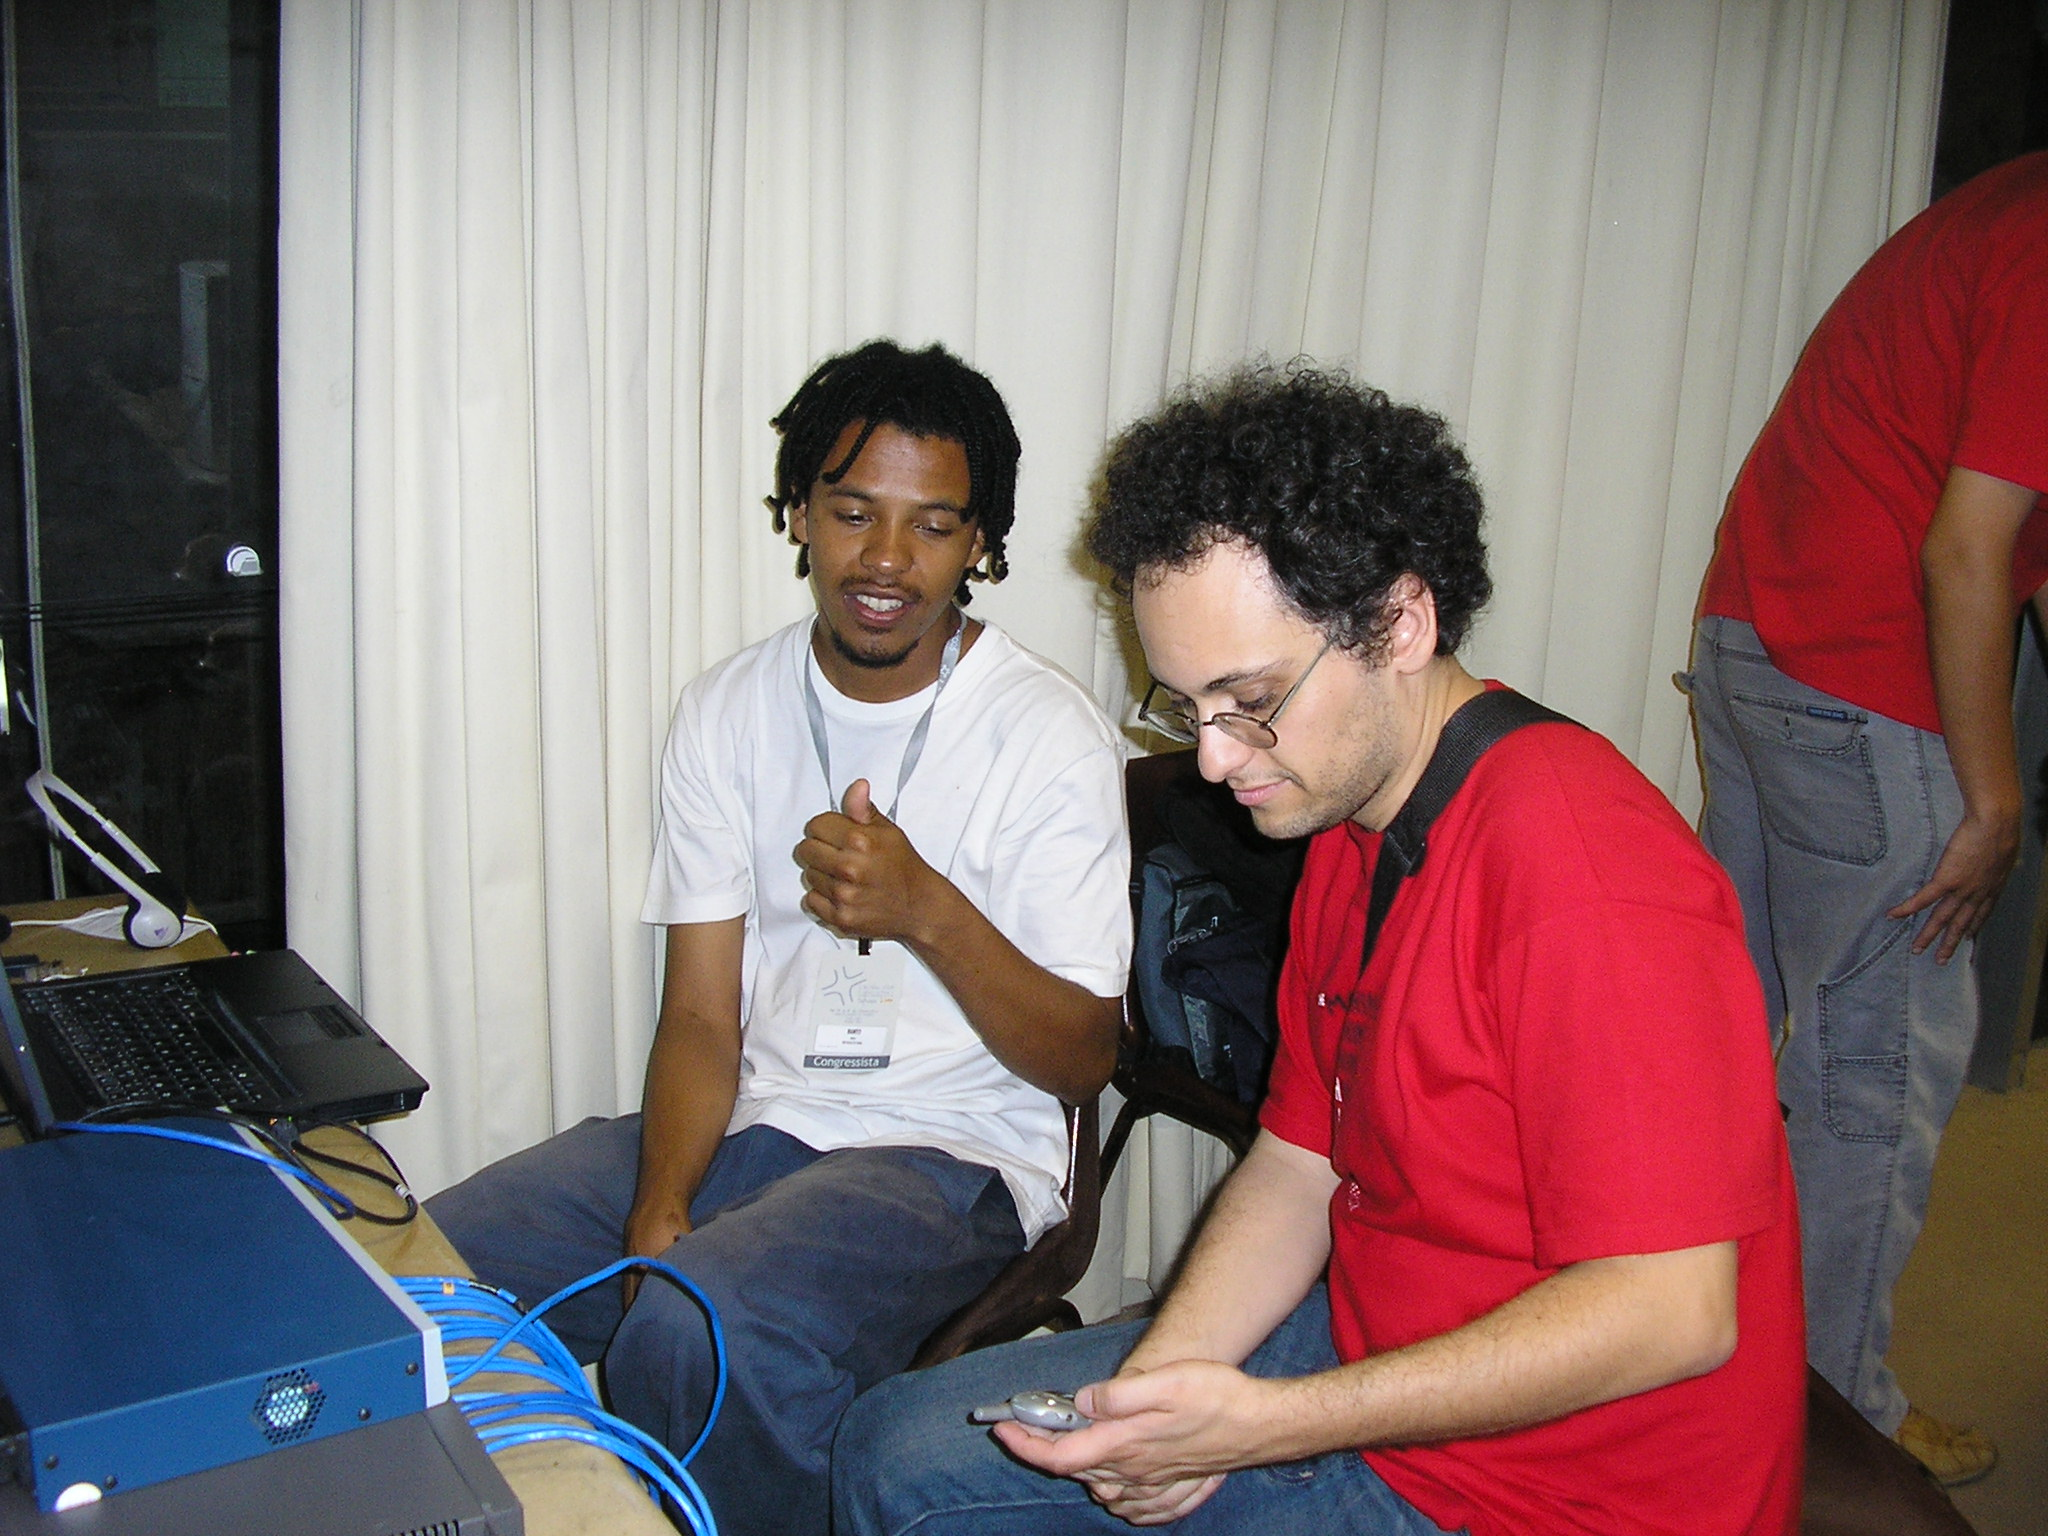
\includegraphics[width=1.0\linewidth]{../../imagens/bantorafa.JPG}
                \caption{Oficina de forma\c{c}\~ao de implementadores(as). Na foto v\^e-se Rafael Gomes da Cruz (i.e. Banto Palmarino). Banto foi posteriormente integrado `a equipe do WASH, trazendo para o novo programa a experi\^encia de multiplica\c{c}\~ao do GESAC.}
                \label{d2d74ac61c1b95a746858e8420d24348e1b48f51}
\end{minipage}%
\hspace{0.5cm}
\begin{minipage}[b]{0.4\linewidth}
        \centering
                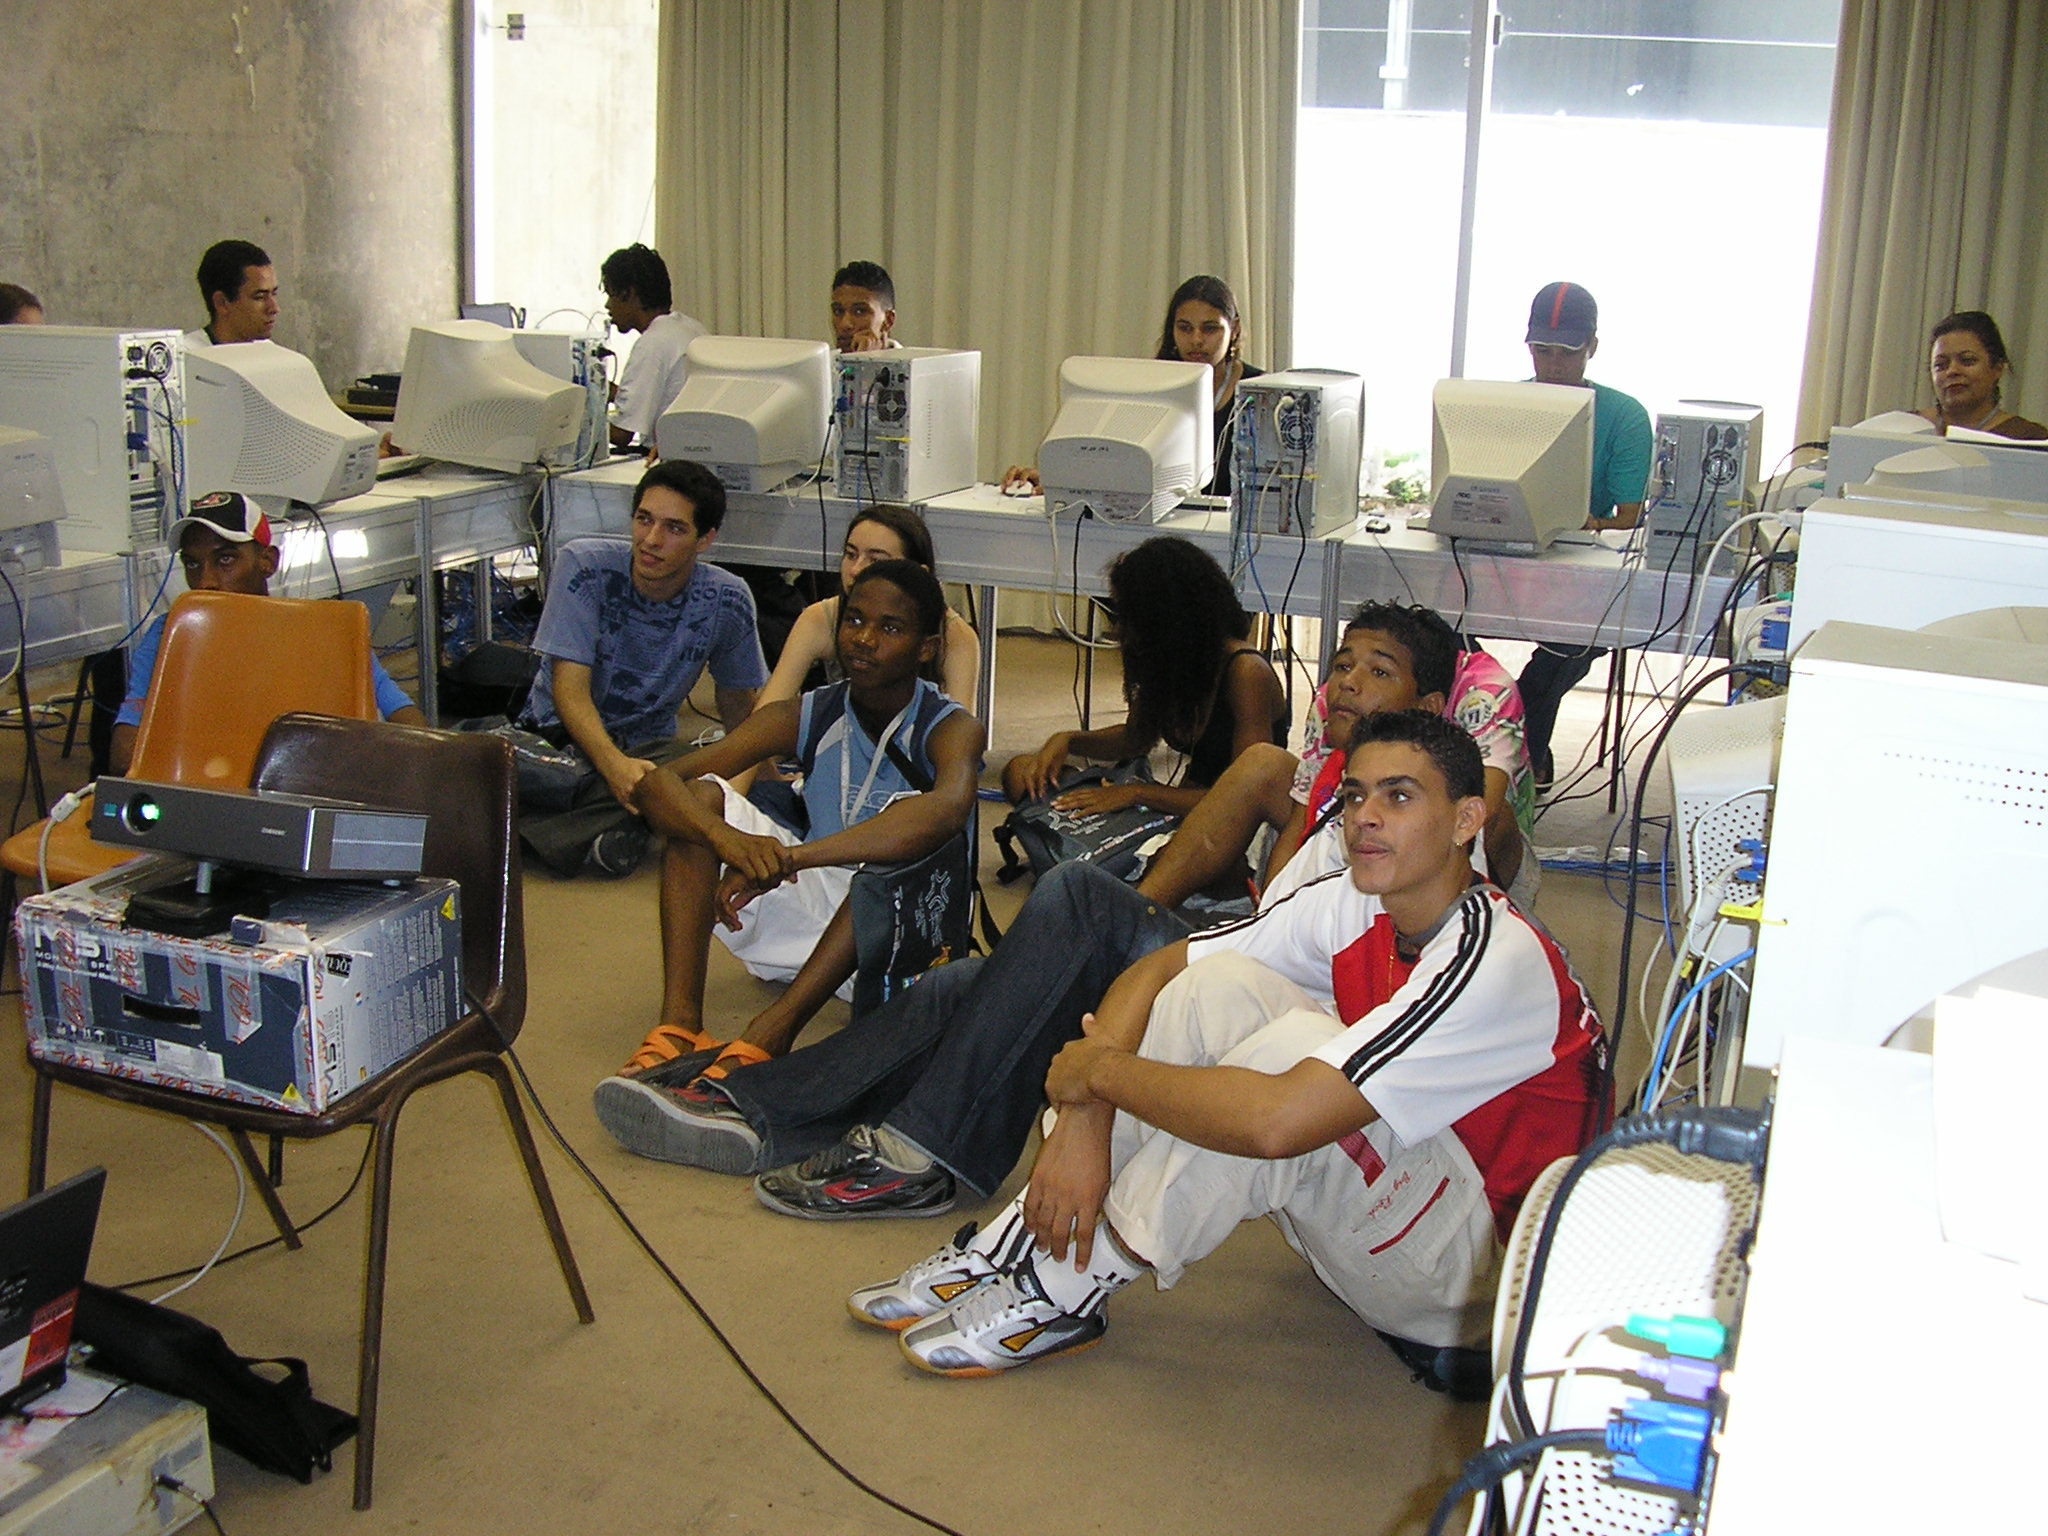
\includegraphics[width=1.0\linewidth]{../../imagens/oficinalac.JPG}
                \caption{Oficina LacFree do GESAC, baseada sempre em conhecimentos livres.}
                \label{350ae75fda8eb19905317e70b64079af869125d8}
\end{minipage}
\hspace{0.5cm}
\begin{minipage}[b]{0.4\linewidth}
        \centering
                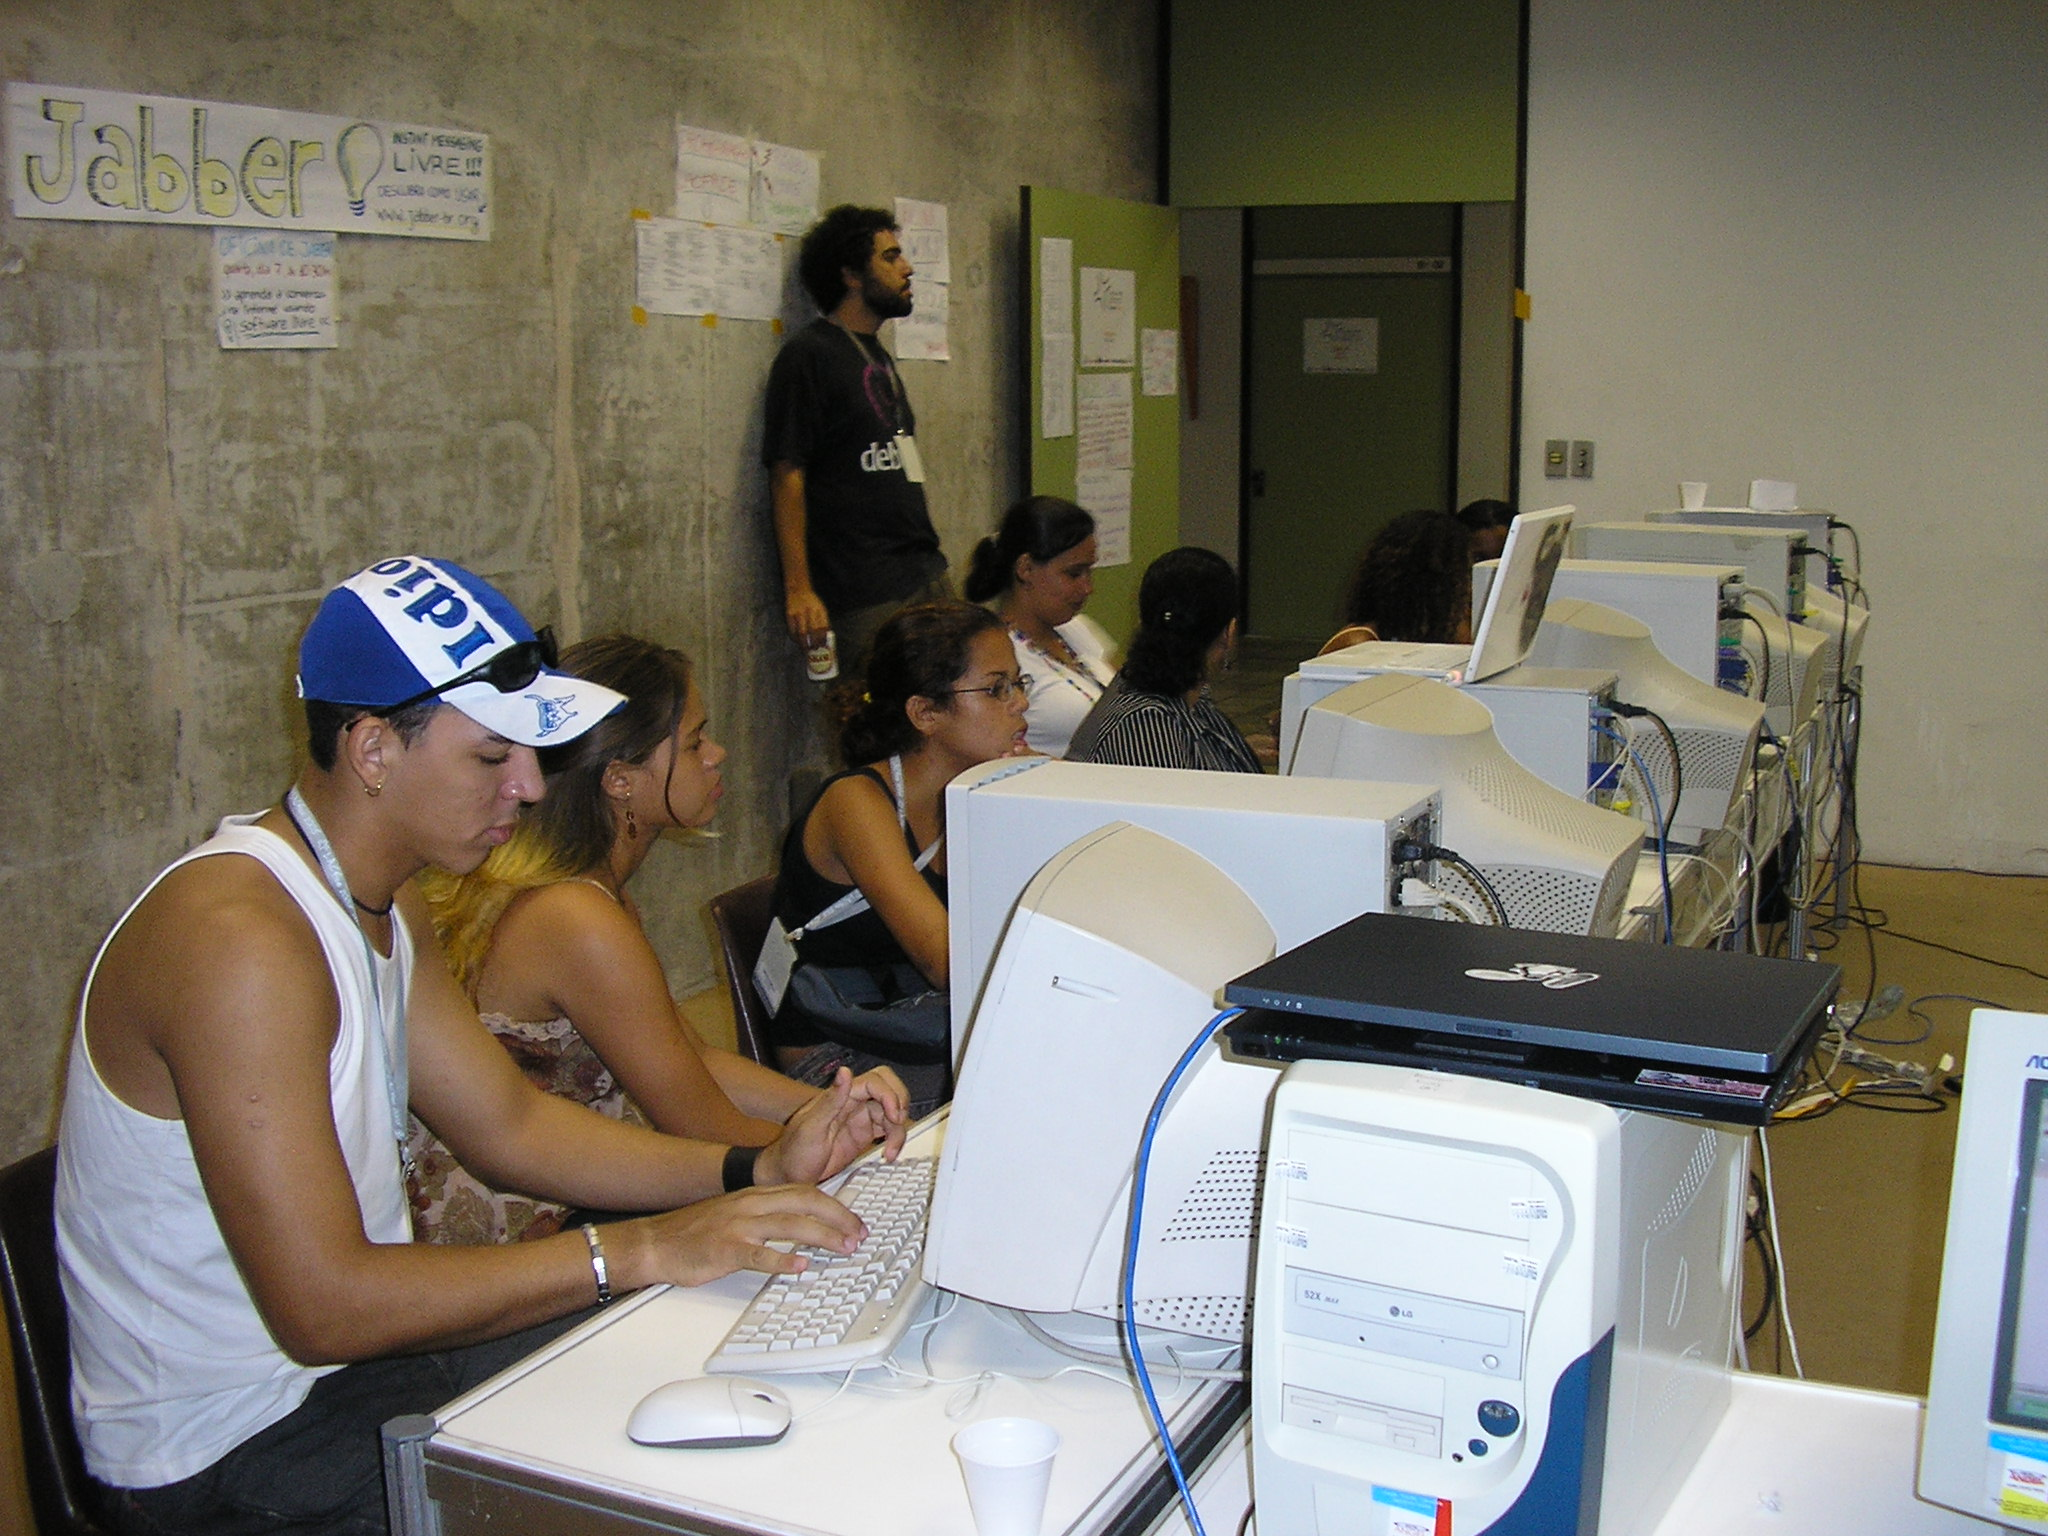
\includegraphics[width=1.0\linewidth]{../../imagens/jabber.JPG}
                \caption{Oficina de Jabber com gestores.}
                \label{e29d9c3f5a4aa82fa420bc60ed161880a24bc2b6}
\end{minipage}%
\hspace{0.5cm}
\begin{minipage}[b]{0.4\linewidth}
        \centering
                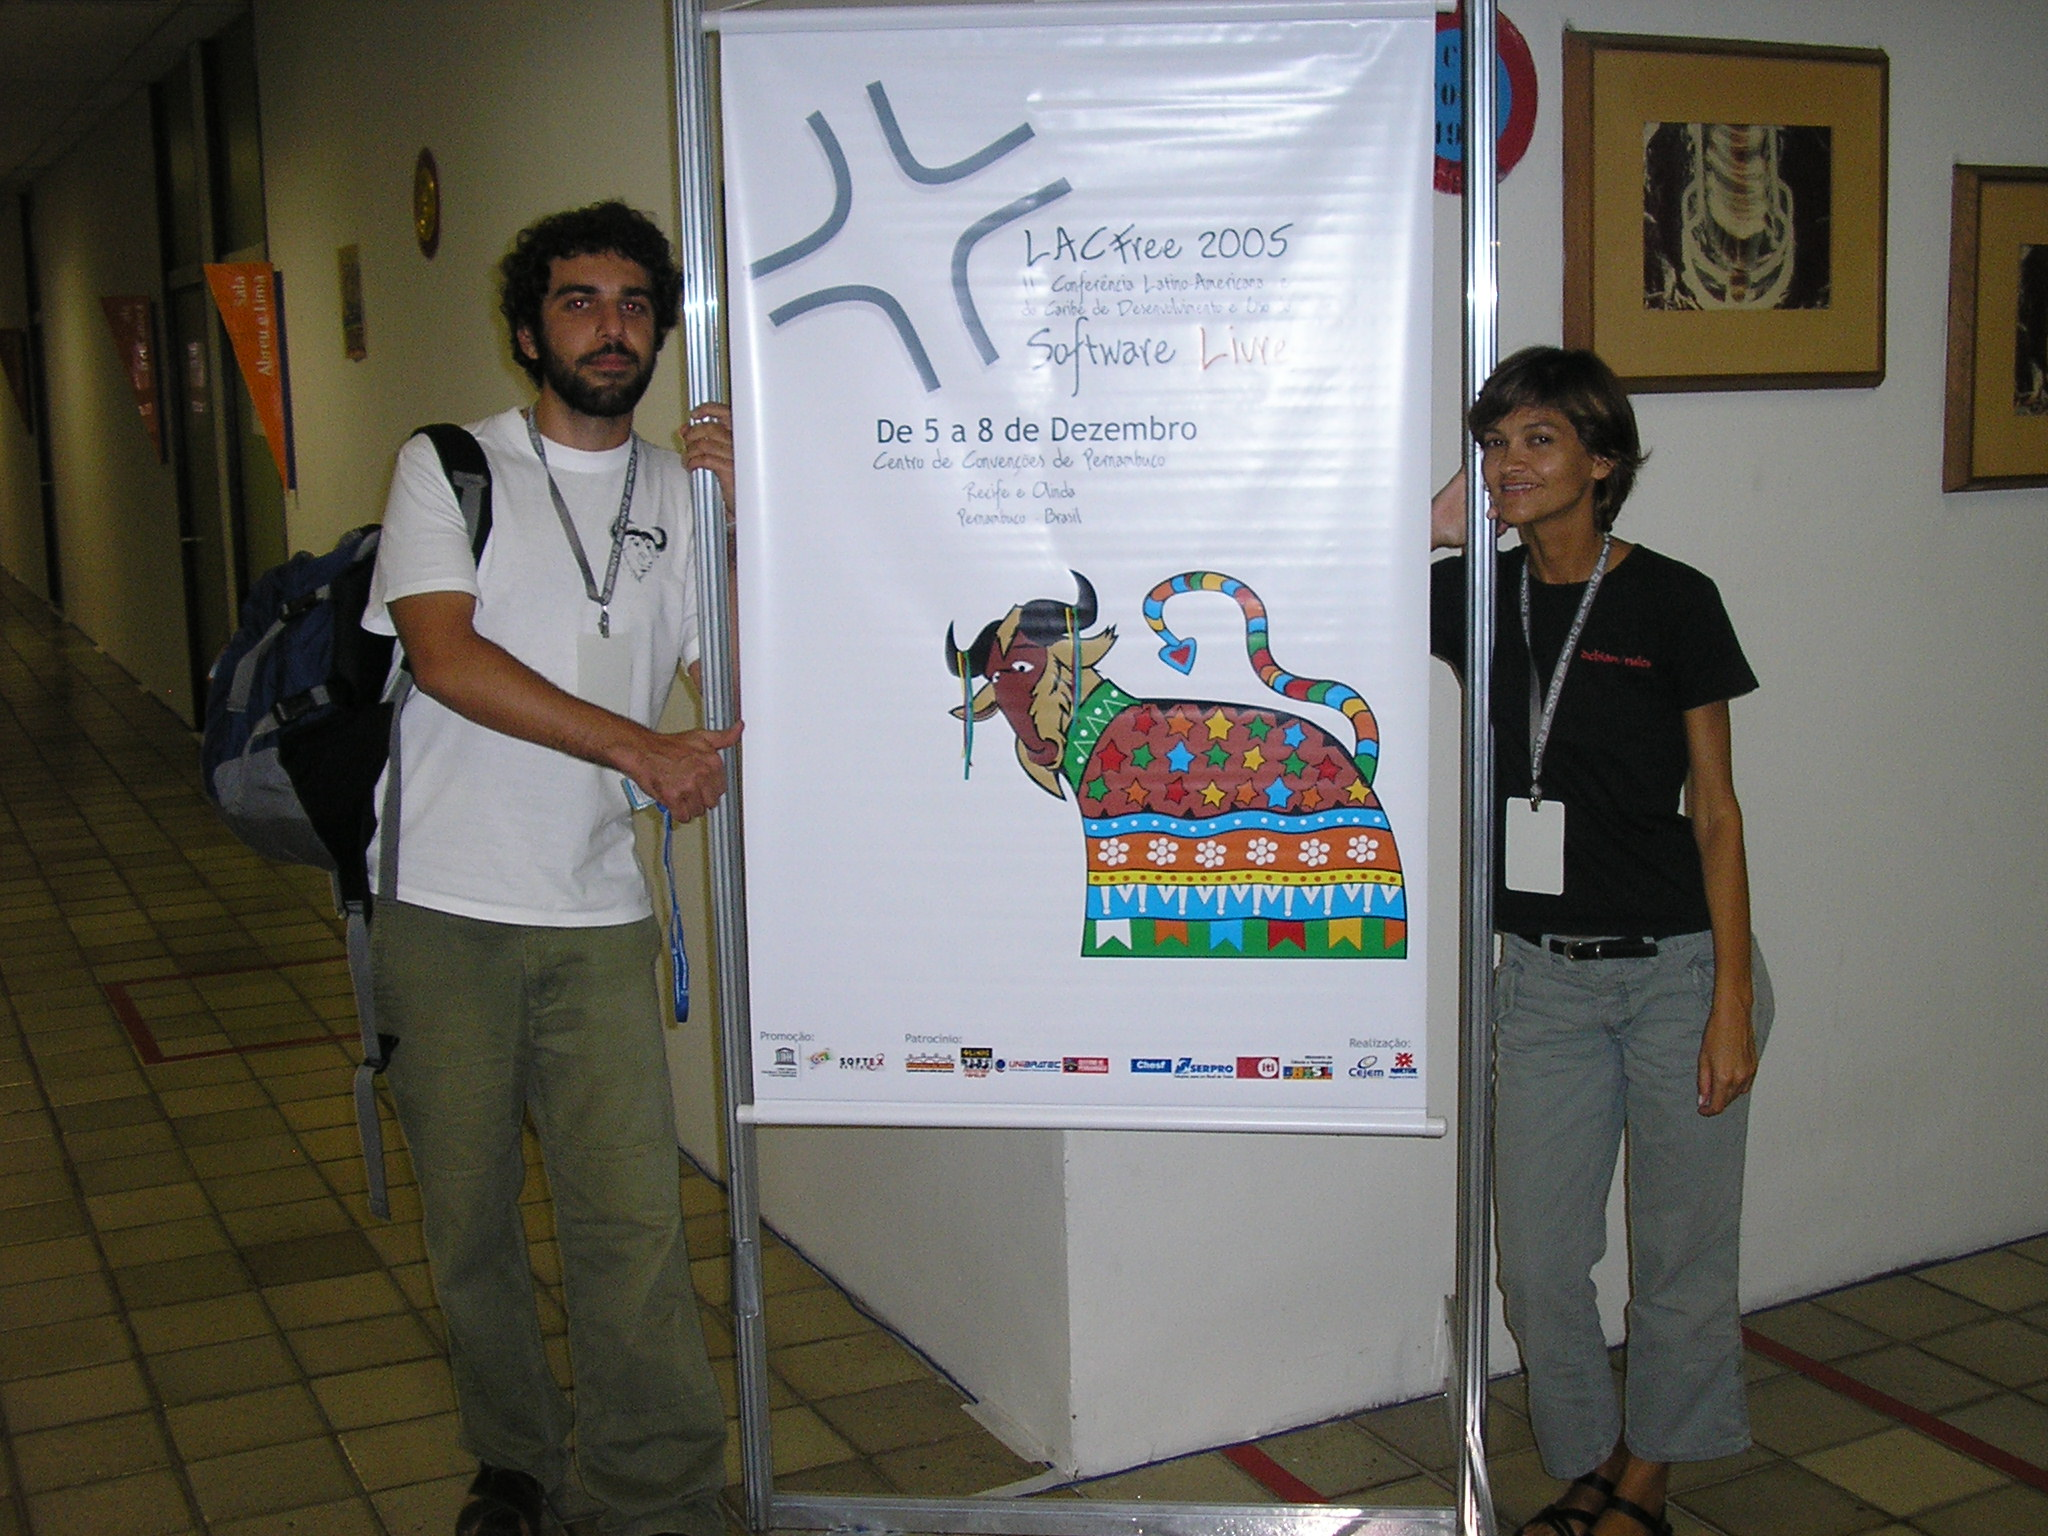
\includegraphics[width=1.0\linewidth]{../../imagens/lacelavince.JPG}
                \caption{A presente autora, ao lado de Vincenzo Tozzi, implementador que tamb\'em veio a contribuir com o WASH.}
                \label{4459669909728990ef00df4bdb6a369f3449704e}
\end{minipage}
\hspace{0.5cm}
\begin{minipage}[b]{0.4\linewidth}
        \centering
                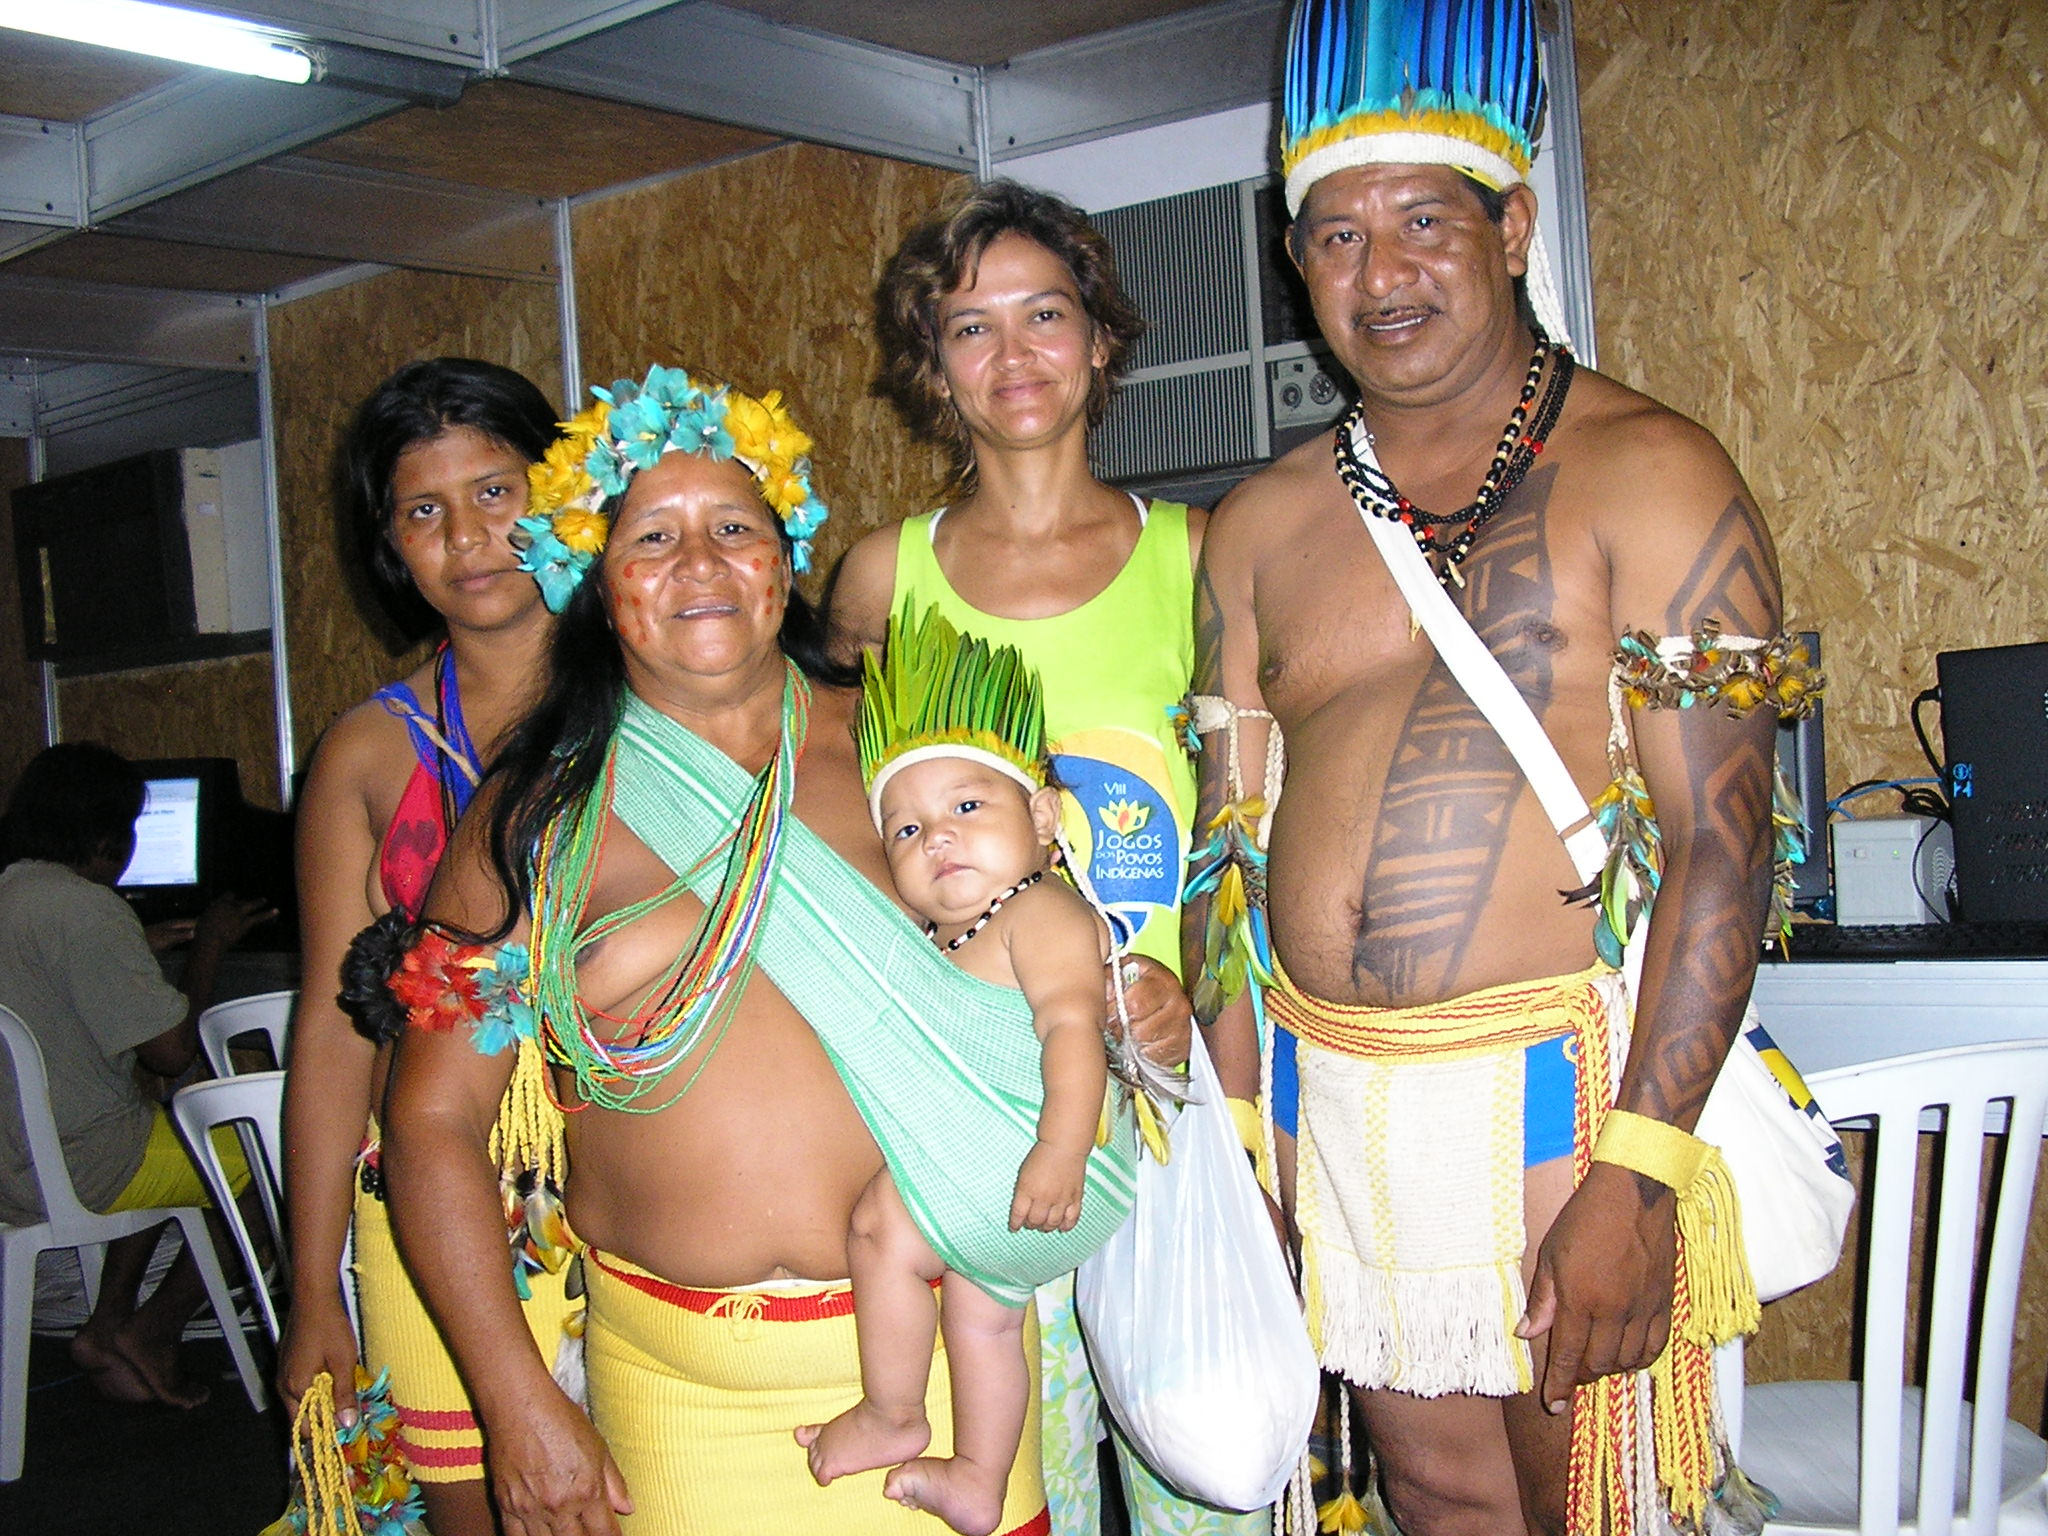
\includegraphics[width=1.0\linewidth]{../../imagens/povo.JPG}
                \caption{Oficinas em comunidades ind\'{i}genas eram muito comuns no GESAC.}
                \label{50c13a4f82feece9e41db915d8e5bc4c5d5094dd}
\end{minipage}%
\hspace{0.5cm}
\end{figure}



\subsection[A avalia\c{c}\~ao do OLPC pelo CTI como g\^enese do WASH]{A avalia\c{c}\~ao do OLPC pelo CTI como g\^enese do WASH}\label{A avalia\c{c}\~ao do OLPC pelo CTI como g\^enese do WASH}
Nesta se\c{c}\~ao fazemos uma interpreta\c{c}\~ao sobre a g\^enese do Programa WASH, a partir do acervo de documentos por n\'os levantado. Foram utilizados, principalmente  os documentos referentes a duas avalia\c{c}\~oes conduzidas pelo coordenador do Programa WASH, na primeira d\'ecada deste s\'eculo:













\begin{alineas}
\item Avalia\c{c}\~ao do Projeto \textquotedbl\{\}One Laptop per Child\textquotedbl\{\} (OLPC) e sua vers\~ao brasileira, \textquotedbl\{\}Projeto Um Computador por Aluno\textquotedbl\{\} (UCA)  (MAMMANA, 2006)
\item Avalia\c{c}\~ao do Programa de Inclus\~ao Digital (PID) da Secretaria de Inclus\~ao Social do Minist\'erio da Ci\^encia e Tecnologia  (CGEE, 2010a)
\end{alineas}

Al\'em dos documentos citados, a presente se\c{c}\~ao se baseou em entrevistas com o Dr. Victor Pellegrini Mammana.












O Projeto \textquotedbl\{\}One Laptop Per Child\textquotedbl\{\} (NEGROPONTE, 2004) foi uma das iniciativas mais completas e robustas no sentido de ampliar a escala de aplica\c{c}\~ao das ideias de Papert. Ao mesmo tempo, era bastante pol\^emica, (ALVAREZ, 2015) por suas caracter\'{\i}sticas disruptivas, alcance e ambi\c{c}\~ao de crescimento, simultaneamente a uma certa desestrutura\c{c}\~ao que prejudicava a confian\c{c}a dos gestores p\'ublicos em sua viabilidade (MAMMANA e TOZZI, 2018).












Embora o Projeto OLPC estivesse no \^ambito de uma Organiza\c{c}\~ao n\~ao Governamental independente,  foi concebido por pesquisadores do Massachusetts Institute of Technology (MIT), apoiados nas ideias e experi\^encias de Seymour Papert  (ALVAREZ, 2015). Especificamente, o Projeto OLPC \'e resultado das ideias debatidas por muitos anos no Media Lab, laborat\'orio do MIT, do qual Papert foi Presidente do Conselho e Co-Fundador  (ALVAREZ, 2015).












Os proponentes do OLPC tinham a ambi\c{c}\~ao de que suas ideias fossem adotadas por pa\'{\i}ses em desenvolvimento e, para isso, estabeleceram planos para regi\~oes espec\'{\i}ficas do mundo, a exemplo do Brasil.












Em 2005, Nicholas Negroponte, idealizador do Projeto OLPC, apresentou sua ideia em Davos (MARKOFF, 2005). Naquela oportunidade, encontrou-se com representantes do Governo Brasileiro (ALVAREZ, 2015) que organizaram um encontro com o presidente Lula, o qual foi realizado em junho daquele ano (ALVAREZ, 2015) (CRISTINA, 2005).












Como resultado dessas tratativas iniciais, o documento intitulado \textquotedbl\{\}Brazil Plan \textquotedbl\{\}  (NEGROPONTE, 2004), fonte prim\'aria para a constru\c{c}\~ao da presente narrativa, foi direcionado \`a \textquotedbl\{\}Brazilian Task Force\textquotedbl\{\}, tendo sido compartilhado com o governo brasileiro, em 2005.












O OLPC era explicitamente apoiado por Papert, quando ainda estava vivo, tendo contado com sua presen\c{c}a ativa e eloquente nas reuni\~oes de apresenta\c{c}\~ao do OLPC para o Governo Brasileiro, inclusive em uma visita ao presidente Lula (ver Fig. 21).














\captionsetup{format=plain}
\begin{figure}[max size={\textwidth}{\textheight}]

\centering


\begin{minipage}[b]{0.4\linewidth}
        \centering
                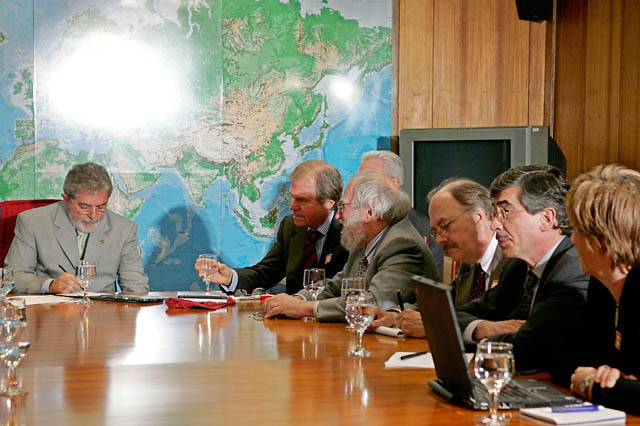
\includegraphics[width=1.0\linewidth]{../../imagens/lula-papert.jpg}
                \caption{Presidente Lula, Negroponte, Papert, Rodrigo Mesquita e Mary Lou Kepsen (fonte: flicker de Rodrigo Mesquita).}
                \label{7c0febad22b3e599a6886b31cdcbd3be3ce60df2}
\end{minipage}%
\hspace{0.5cm}
\begin{minipage}[b]{0.4\linewidth}
        \centering
                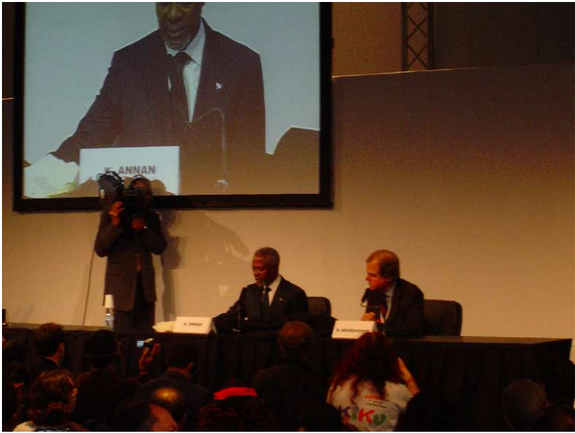
\includegraphics[width=1.0\linewidth]{../../imagens/Kofi-negroponte.png}
                \caption{Nicholas Negroponte apresentando o prot\'otipo do OLPC para o Secret\'ario Geral da ONU, Kofi Anan (cr\'edito: Victor Mammana, 2005).}
                \label{31f6206a8e4662597d5a134974d64a4696f4129c}
\end{minipage}
\hspace{0.5cm}
\begin{minipage}[b]{0.4\linewidth}
        \centering
                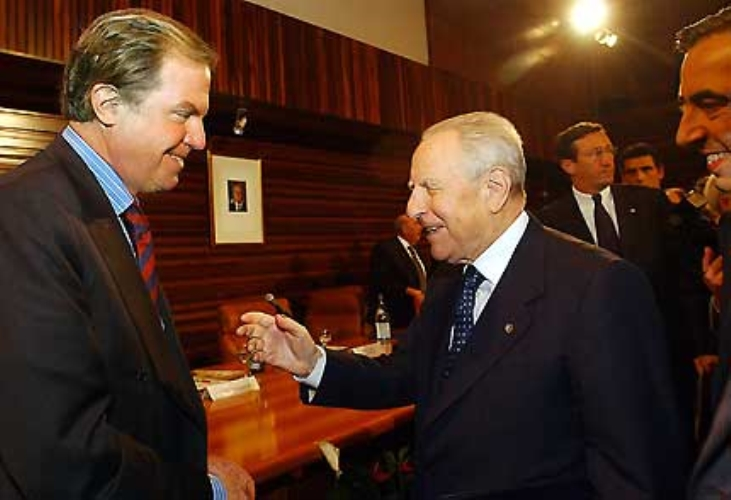
\includegraphics[width=1.0\linewidth]{../../imagens/presidente-italia.jpg}
                \caption{Nicholas Negroponte com o presidente da It\'alia, em 2003.}
                \label{f15f5d2fa7b78d2e6dec6ac4a7be76d564c9bf71}
\end{minipage}%
\hspace{0.5cm}
\begin{minipage}[b]{0.4\linewidth}
        \centering
                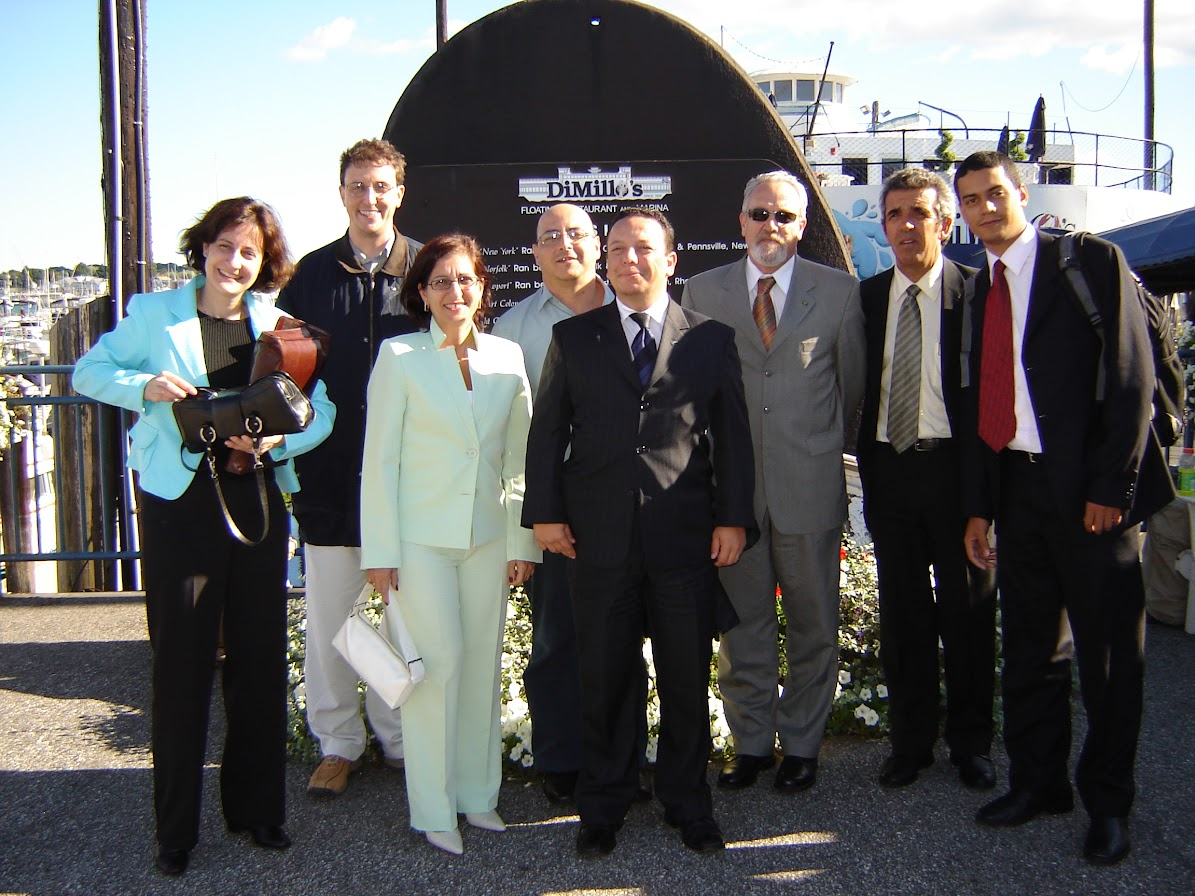
\includegraphics[width=1.0\linewidth]{../../imagens/equipeOLPC.jpg}
                \caption{Miss\~ao Brasileira de avalia\c{c}\~ao da proposta OLPC, em visita ao Maine em 2005. (fonte: acervo pessoal)}
                \label{b1b538b3cf66c3aaf3d7a74aac4332a1f40be14d}
\end{minipage}
\hspace{0.5cm}
\end{figure}



Nicholas Negroponte, o l\'{\i}der da iniciativa do OLPC, era um destacado \textquotedbl\{\}guru \textquotedbl\{\} tecnol\'ogico, professor do MIT, cofundador da revista Wired e tinha acesso a chefes de estado, a exemplo do presidente Miterrand, da Fran\c{c}a que, na d\'ecada de 80, foi apoiador da cria\c{c}\~ao do \textquotedbl\{\}Centre mondial informatique et ressource humaine\textquotedbl\{\}, onde Negroponte atuou como dirigente. Coincidentemente, era irm\~ao de John Negroponte, ent\~ao Secret\'ario de Estado do Governo Bush, diplomata americano influente nos meios pol\'{\i}ticos, na comunidade de informa\c{c}\~ao e em outras \'areas estrat\'egicas e de defesa daquele pa\'{\i}s.












A refer\^encia ao \textquotedbl\{\}Centre mondial informatique et ressource humaine\textquotedbl\{\} assume uma particular import\^ancia nesta narrativa, uma vez que um outro part\'{\i}cipe desta hist\'oria, o Prof. Jose Ellis Ripper Filho (esposo da Profa. Afira Ripper) foi membro do conselho dessa institui\c{c}\~ao francesa, estabelecendo um emaranhado de rela\c{c}\~oes entre seus atores, ao longo de v\'arias d\'ecadas. No per\'{\i}odo em que atuou como conselheiro, a convite de Miterrand, o Prof. Ripper chegou a interagir diretamente com Negroponte, muito antes da concep\c{c}\~ao do OLPC.












Nicholas transitava com razo\'avel desenvoltura entre l\'{\i}deres mundiais, a exemplo de Kofi Anan (ver Fig. 22), Lula (ver Fig. 21), Mitterrand ou o presidente da It\'alia (ver Fig. 23). Essa presen\c{c}a junto a governos criou a oportunidade para que, em 2006, pa\'{\i}ses como Argentina, Nig\'eria, China, \'India, Egito e Costa Rica participassem das tratativas do OLPC  (p\'ag. 84 de ALVAREZ, 2015).












A proposta era ousada e atraente no que tange \`a transforma\c{c}\~ao dos m\'etodos pedag\'ogicos. Por outro lado, era tamb\'em exigente em termos de recursos, uma vez que preconizava a aquisi\c{c}\~ao de milh\~oes de notebooks como forma de empoderamento dos estudantes pela possibilidade de conex\~ao \`a internet  (NEGROPONTE, 2004). Em termos or\c{c}ament\'arios, a ades\~ao \`a proposta de Negroponte representava um valor significativo do or\c{c}amento do Minist\'erio da Educa\c{c}\~ao (cerca de quatro bilh\~oes de d\'olares) e havia o entendimento do governo brasileiro de que, para que fosse viabilizado no pa\'{\i}s, o OLPC precisaria passar por um escrut\'{\i}nio da sociedade brasileira.












Ciente do risco que representava uma ades\~ao voluntariosa a um programa t\~ao disruptivo, a Presid\^encia da Rep\'ublica da \'epoca decidiu estabelecer um grupo de avalia\c{c}\~ao  daquela proposta, o  qual foi constitu\'{\i}do por universidades e centros de pesquisa. Foram chamados o Centro de Tecnologia da Informa\c{c}\~ao Renato Archer (CTI), a Escola Polit\'ecnica da USP e a Funda\c{c}\~ao CERTI (ALVAREZ, 2015). A Fig. 24 traz uma imagem de uma parte da miss\~ao brasileira, constitu\'{\i}da para avaliar o OLPC, em visita ao Maine em 2005.












Coordenavam as atividades de avalia\c{c}\~ao, o assessor especial da Presid\^encia da Rep\'ublica, Dr. C\'esar Santos Alvarez, e o secret\'ario de Pol\'{\i}tica de Inform\'atica, Dr. Marcelo Lopes.












O grupo de tr\^es entidades de pesquisa tinha como intuito:













\noindent\begin{center}\mbox{\centering\fbox{\centering\par\parbox{0.7\linewidth}{\small\textit{\textquotedbl\{\}verificar sua adequa\c{c}\~ao (OLPC) \`a realidade nacional dentro das expectativas do governo de investir em processos de melhoria da qualidade da educa\c{c}\~ao brasileira\textquotedbl\{\}  (MEC, 2006 apud ALVAREZ, 2015)}\normalsize}}}\end{center}


As institui\c{c}\~oes mencionadas avaliaram o projeto em v\'arios aspectos  (MAMMANA, 2005a):













\begin{alineas}
\item proposta pedag\'ogica;
\item modelo de neg\'ocios;
\item cadeia de fornecimento;
\item sistema de qualidade;
\item produ\c{c}\~ao;
\item software;
\item ergonomia;
\item certifica\c{c}\~ao e normas t\'ecnicas;
\item displays;
\item mock-ups;
\item usabilidade;
\item arquitetura de refer\^encia;
\item avalia\c{c}\~ao experimental; e
\item rede.
\end{alineas}

A proposta previa a aquisi\c{c}\~ao de um \textquotedbl\{\}laptop\textquotedbl\{\} por estudante brasileiro, ou seja, perto de 30 a 40 milh\~oes de unidades.












Segundo a vis\~ao trazida pelo OLPC  (NEGROPONTE, 2004) ao governo brasileiro, a disponibiliza\c{c}\~ao em larga escala de acesso \`a internet alteraria a rela\c{c}\~ao aluno-professor, promovendo formas de aprendizagem alternativas ao conteudismo tradicional, reformulando tamb\'em o formato lousa-giz inerente ao sistema educacional brasileiro.












Um dos aspectos principais do projeto apresentado ao governo, do ponto de vista de software, era a disponibiliza\c{c}\~ao de uma ferramenta de programa\c{c}\~ao mais intuitiva e l\'udica do que o pr\'oprio LOGO, linguagem criada por Papert e colegas na d\'ecada de 60 e que se disseminou por todo o mundo (ver Fundamenta\c{c}\~ao Te\'orica).












Das tr\^es institui\c{c}\~oes envolvidas na avalia\c{c}\~ao do OLPC, tivemos acesso \`a avalia\c{c}\~ao do CTI  (MAMMANA e TOZZI, 2018), que ficou encarregado da:













\begin{alineas}
\item avalia\c{c}\~ao de caracter\'{\i}sticas de ergonomia postural, por meio da captura de movimento;
\item avalia\c{c}\~ao de caracter\'{\i}sticas de ergonomia sensorial, por meio de t\'ecnicas relacionadas \`a \'area de mostradores de informa\c{c}\~ao;
\item avalia\c{c}\~ao da funcionalidade dos \textquotedbl\{\}laptops\textquotedbl\{\}, principalmente em termos de redes, processamento, mem\'oria e baterias;
\item avalia\c{c}\~ao do emprego dos dispositivos  da escola p\'ublica;
\item avalia\c{c}\~ao da percep\c{c}\~ao dos professores sobre o projeto;
\item an\'alise da infraestrutura das escolas, visando verificar a viabilidade de implanta\c{c}\~ao do projeto;
\item acompanhamento de pilotos de avalia\c{c}\~ao em escolas p\'ublicas brasileiras; e
\item visitas a pilotos nos Estados Unidos.
\end{alineas}

Do ponto de vista da aquisi\c{c}\~ao de \textquotedbl\{\}laptops \textquotedbl\{\} em larga escala, o CTI identificou uma s\'erie de dificuldades nas seguintes \'areas: apropria\c{c}\~ao pela escola brasileira, produ\c{c}\~ao dos laptops, restri\c{c}\~oes or\c{c}ament\'arias, falta de vis\~ao clara sobre o controle dos conte\'udos, falta de uma vis\~ao sobre capacita\c{c}\~ao dos profissionais da educa\c{c}\~ao, problemas ergon\^omicos e, principalmente, obsolesc\^encia dos equipamentos  (MAMMANA e TOZZI, 2018). Estes aspectos demonstraram que a ideia de aquisi\c{c}\~ao de milh\~oes de laptops representava um risco muito grande para o sistema educacional brasileiro.












O estudo apontava, tamb\'em, que o sistema educacional poderia se beneficiar de alguns aspectos da proposta, mas que qualquer iniciativa disruptiva no sistema educacional brasileiro requereria mais investimentos em capacita\c{c}\~ao de recursos humanos do que em hardware ou software, ao contr\'ario do que propunha o Projeto OLPC, que focalizava a aquisi\c{c}\~ao dos computadores.












A percep\c{c}\~ao de que o Projeto OLPC, como proposto por Negroponte, tinha um equ\'{\i}voco em seu foco foi expressa principalmente pela equipe do CTI, que se destacou dos demais participantes da avalia\c{c}\~ao, que estavam mais propensos a apoiar o projeto como originalmente proposto. A posi\c{c}\~ao do CTI se sustentava na pr\'opria defini\c{c}\~ao de educa\c{c}\~ao empregada na an\'alise da proposta OLPC: \textquotedbl\{\}Educa\c{c}\~ao \'e a inser\c{c}\~ao do indiv\'{\i}duo em sua pr\'opria cultura, atrav\'es da intera\c{c}\~ao com outros indiv\'{\i}duos\textquotedbl\{\}.












Esta defini\c{c}\~ao colocava a intera\c{c}\~ao entre indiv\'{\i}duos no centro do processo e, portanto, qualquer esfor\c{c}o de qualifica\c{c}\~ao da escola brasileira precisaria passar por uma \^enfase no investimento em \textquotedbl\{\}pessoas, mais do que em software ou hardware \textquotedbl\{\}.












A proposta do MIT envolvia abordagens pedag\'ogicas que buscavam combinar elementos de um amplo espectro de correntes distintas, que partiam de Piaget, passando por Vygotsky, Dewey e chegando em Paulo Freire  (NEGROPONTE, 2004).












N\~ao obstante essa pluralidade conceitual, o documento do OLPC n\~ao escondia a preval\^encia do pensamento de Papert (que na \'epoca ainda era vivo) na concep\c{c}\~ao da proposta apresentada ao Governo Brasileiro.













\noindent\begin{center}\mbox{\centering\fbox{\centering\par\parbox{0.7\linewidth}{\small\textit{(...) um dos aspectos mais atraentes da proposta \'e a \^enfase em “estrat\'egias para aprender o que n\~ao se sabe” ao inv\'es de focalizar “em ensinar o que os outros devem saber”. Esta mudan\c{c}a de foco no processo educacional, segundo os argumentos apresentados, seria poss\'{\i}vel atrav\'es do emprego de dispositivos digitais port\'ateis conectados \`a internet, que devem superar os problemas oriundos de t\'ecnicas tradicionais de ensino. O programa, segundo o MIT, oferece uma solu\c{c}\~ao para os problemas que “foram formulados (mas, talvez, nunca resolvidos) por Jean Piaget, Paulo Freire, John Dewey e Lev Vygotsky”. (Fonte: tradu\c{c}\~ao livre de NEGROPONTE (2004))}\normalsize}}}\end{center}


Um outro aspecto do programa era o foco na \textquotedbl\{\}propriedade de um bem de inform\'atica em detrimento do compartilhamento destes recursos em um laborat\'orio de computadores\textquotedbl\{\}. A vis\~ao da \'epoca considerava que a doa\c{c}\~ao de um laptop com acesso irrestrito \`a internet deveria ser a base de um novo processo educacional  (MAMMANA, 2006). Este enfoque buscava enfrentar uma defici\^encia de programas anteriores como o Proinfo do MEC, que por ser desprovido de uma vis\~ao pedag\'ogica estruturada sobre o uso de computadores, deixando o controle de acesso aos laborat\'orios para profissionais sem uma capacita\c{c}\~ao espec\'{\i}fica, resultou em uma profus\~ao de relatos de \textquotedbl\{\}laborat\'orios de micros trancados\textquotedbl\{\} (ver Fig. 25)  (CNPq, 2020b). No OLPC n\~ao existiria restri\c{c}\~ao de acesso aos computadores, porque os donos dos equipamentos eram os pr\'oprios estudantes. Mas, esta \textquotedbl\{\}vantagem\textquotedbl\{\} n\~ao trazia luz sobre  uma quest\~ao que surgiria imediatamente ap\'os a doa\c{c}\~ao do laptop para a crian\c{c}a: v\~ao fazer o que com isso?














\captionsetup{format=plain}
\begin{figure}[htb]

	\begin{center}

		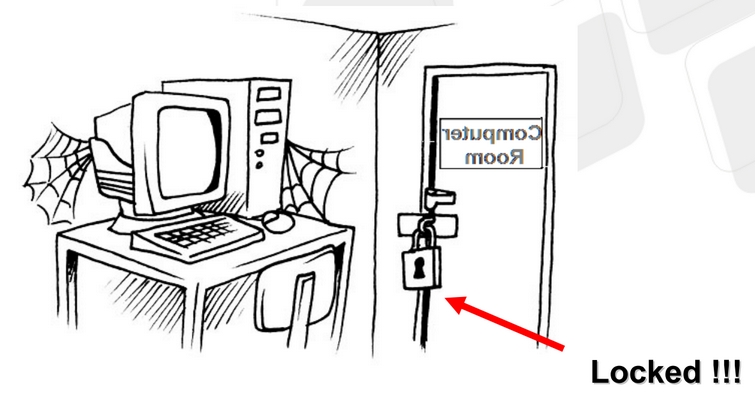
\includegraphics[max size={\textwidth}{\textheight}]{../../imagens/computer-room.png}

	\end{center}

	\caption{\label{5817b264c8a300b4b46214039b2e579aba5d70a7}Arte produzida sob encomenda para a avalia\c{c}\~ao do OLPC, expondo a situa\c{c}\~ao dos laborat\'orios de micro-computadores de muitas escolas brasileiras no final de s\'eculo XX, in\'{i}cio do XXI. (Fonte: acervo pessoal de Victor Mammana)}

\end{figure}

A avalia\c{c}\~ao do Governo Brasileiro j\'a percebia que o OLPC exagerava o papel que uma simples ferramenta digital (laptop) poderia desempenhar no processo educacional, mas reconhecia que o uso desta ferramenta na escola poderia \textquotedbl\{\}permitir uma melhor prepara\c{c}\~ao para a sobreviv\^encia do educando na sociedade de informa\c{c}\~ao, criando oportunidades para sua inclus\~ao como membro ativo desta sociedade\textquotedbl\{\}.












Mas, o proleto tamb\'em criava muita inseguran\c{c}a nas autoridades brasileiras e, a partir de agora, citamos algumas com base nos achados descritos por MAMMANA (2006) em seu relat\'orio final de avalia\c{c}\~ao, concentrando-nos em quest\~oes de cunho estrat\'egico e geopol\'{\i}tico:













\begin{alineas}
\item \textquotedbl\{\}Em \'ultima an\'alise, o OLPC \'e um projeto de poder, com m\'eritos e agendas alternativas \`as dos Estados Nacionais, que atua na \'area mais sens\'{\i}vel de qualquer sociedade: sua reprodu\c{c}\~ao e reinven\c{c}\~ao, ou seja, a educa\c{c}\~ao;\textquotedbl\{\}
\item \textquotedbl\{\}A ades\~ao ao OLPC coloca a internet no centro do processo de aprendizagem, promovendo a converg\^encia final entre educa\c{c}\~ao e m\'{\i}dia; \textquotedbl\{\}
\item \textquotedbl\{\}A despeito de qualquer paran\'oia, a previs\~ao de qual \'e a dire\c{c}\~ao e evolu\c{c}\~ao do controle da internet \'e objeto de muita controv\'ersia em todos os meios, mas deve ser tema de reflex\~ao por parte das autoridades que decidir\~ao pela ades\~ao ao OLPC, pela relev\^ancia que a mesma assume no contexto do programa;\textquotedbl\{\}
\item \textquotedbl\{\}O que deve ser evitado pelo governo brasileiro \'e a ades\~ao extempor\^anea a um projeto cuja a agenda \'e controlada por grupos que n\~ao est\~ao sob a esfera de influ\^encia do poder democr\'atico, institu\'{\i}do em nosso pa\'{\i}s;\textquotedbl\{\}
\item \textquotedbl\{\}Mais do que a converg\^encia de tecnologias de informa\c{c}\~ao e comunica\c{c}\~ao (TICs), a proposta OLPC traz, em si, a converg\^encia da m\'{\i}dia com a educa\c{c}\~ao, quando esta \'ultima passa a ser, definitivamente (e pela aus\^encia de uma vis\~ao de cidadania associada), dominada por agentes econ\^omicos globais que custodiam e controlam os conte\'udos que at\'e agora t\^em sido oferecidos democraticamente pela sociedade aos seus reposit\'orios;\textquotedbl\{\}
\item \textquotedbl\{\}Atrav\'es de uma intensa atividade de persuas\~ao nas estruturas de poder de v\'arios pa\'{\i}ses, os representantes da Organiza\c{c}\~ao OLPC, que em parte s\~ao oriundos do Media Lab, v\^em buscando a ades\~ao de diversos governos do mundo para um programa de ado\c{c}\~ao de laptops de baixo custo nas atividades curriculares de suas redes de ensinos fundamental e m\'edio. Simultaneamente, a esta atividade com os governos, \'e razo\'avel acreditar que a Organiza\c{c}\~ao OLPC est\'a, tamb\'em, estabelecendo contratos e acordos que n\~ao t\^em sido divulgados ao p\'ublico e a estes governos. Uma das justificativas para essa n\~ao divulga\c{c}\~ao pode ser a preocupa\c{c}\~ao com for\c{c}as antag\^onicas da ind\'ustria, as quais, por terem seu mercado amea\c{c}ado, podem se utilizar destas informa\c{c}\~oes estrat\'egicas para reagir \`a implementa\c{c}\~ao do OLPC;\textquotedbl\{\}
\item \textquotedbl\{\}A proposta OLPC \'e parcialmente financiada por agentes, que a imprensa frequentemente associa ao universo de think tanks conservadores e ONGs com interesse geopol\'{\i}tico [1], al\'em de empresas de M\'{\i}dia com poss\'{\i}vel interesse no acesso a novos mercados, como \'e o caso da Google; e
\item \textquotedbl\{\}Subjacente a vis\~ao do OLPC est\'a a viabiliza\c{c}\~ao do acesso irrestrito a informa\c{c}\~oes que, se por um lado hoje t\^em diversidade impressionante e acredita-se, est\~ao dispon\'{\i}veis de forma democr\'atica na internet; por outro lado est\~ao sob cust\'odia e escrut\'{\i}nio de estruturas de dissemina\c{c}\~ao de informa\c{c}\~ao dominadas por empresas privadas globais, num modelo de governan\c{c}a da internet que atribui a um \'unico Estado hegem\^onico o poder discricion\'ario sobre toda a rede (ICANN).\textquotedbl\{\}
\end{alineas}

Os pontos levantados pela avalia\c{c}\~ao do OLPC por, parte de pesquisadores brasileiros,levaram a um alerta, seguido de uma recomenda\c{c}\~ao:













\noindent\begin{center}\mbox{\centering\fbox{\centering\par\parbox{0.7\linewidth}{\small\textit{\textquotedbl\{\}(...) Neste contexto, deve ser evitada a ades\~ao extempor\^anea a um projeto cuja a agenda \'e controlada por grupos que n\~ao est\~ao sob a esfera de influ\^encia do poder democr\'atico, institu\'{\i}do em nosso pa\'{\i}s. (...) A impossibilidade de prever o que pode acontecer e a certeza de que existem consequ\^encias para o modelo de democracia brasileiro devem ser o pano de fundo para a tomada de decis\~ao sobre o que fazer com o OLPC. Embora nenhuma a\c{c}\~ao nesta dire\c{c}\~ao tenha sido tomada, sabe-se que h\'a como enquadrar o OLPC naquilo que a sociedade considerar mais conveniente para a cidadania do brasileiro.\textquotedbl\{\} (Fonte:  MAMMANA (2006))}\normalsize}}}\end{center}


Percebe-se, no posicionamento acima, uma preocupa\c{c}\~ao com a possibilidade de forma\c{c}\~ao de estruturas de dissemina\c{c}\~ao de informa\c{c}\~ao em que os valores da cidadania poderiam deixar de ser preponderantes. Em parte, pode-se dizer que as redes sociais de hoje est\~ao se prestando a esse servi\c{c}o, transformando-se em meios para a dissemina\c{c}\~ao de informa\c{c}\~oes falsas, ideologias de \'odio, crimes, entre outros. Interpretando, a posteriori, e por meio de comunica\c{c}\~ao privada recente do autor de uma das avalia\c{c}\~oes, parece-nos que o posicionamento do CTI se insurgia contra a subordina\c{c}\~ao da escola brasileira, ber\c{c}o de nossa cidadania, a esse poder monumental. Talvez o CTI tenha \textquotedbl\{\}farejado\textquotedbl\{\} e antecipado algo que veio a ser testemunhado nos dias de hoje, quando as redes sociais, fora do contexto da escola, se transformaram efetivamente num instrumento de dissemina\c{c}\~ao de informa\c{c}\~oes falsas, teorias da conspira\c{c}\~ao, entre outras formas de cria\c{c}\~ao de realidades paralelas.












Dentre as atividades atribu\'{\i}das a Victor Mammana, no per\'{\i}odo de avalia\c{c}\~ao do OLPC, estava o acompanhamento do desenvolvimento do laptop em si, aproveitando a experi\^encia do mesmo com pol\'{\i}tica industrial na \'area de mostradores de informa\c{c}\~oes (displays). Essa atividade contribuiu para avaliar a viabilidade tecnol\'ogica das solu\c{c}\~oes propostas.












A Fig. 26 mostra uma foto emblem\'atica da situa\c{c}\~ao do desenvolvimento do OLPC, no momento em que o fornecimento dos laptops para o Brasil era negociado, que gerava muita inseguran\c{c}a no Governo Brasileiro. Na foto, tirada por Victor Mammana, \'e poss\'{\i}vel ver que o \textquotedbl\{\}prot\'otipo\textquotedbl\{\} apresentado a Kofi Anan n\~ao tinha \textquotedbl\{\}placa m\~ae\textquotedbl\{\} e n\~ao era um produto real. A eletr\^onica que \textquotedbl\{\}dava vida\textquotedbl\{\} ao mock-up do laptop estava embaixo da mesa. Um extenso relat\'orio foi apresentado ao coordenador da For\c{c}a Tarefa Brasileira de avalia\c{c}\~ao do OLPC, Dr. C\'esar Alvarez, gerando questionamentos \`a equipe do OLPC sobre o real est\'agio de desenvolvimento do prot\'otipo do dito \textquotedbl\{\}laptop de 100 d\'olares, \textquotedbl\{\} naquele crucial momento. (MAMMANA, 2005).














\captionsetup{format=plain}
\begin{figure}[htb]

	\begin{center}

		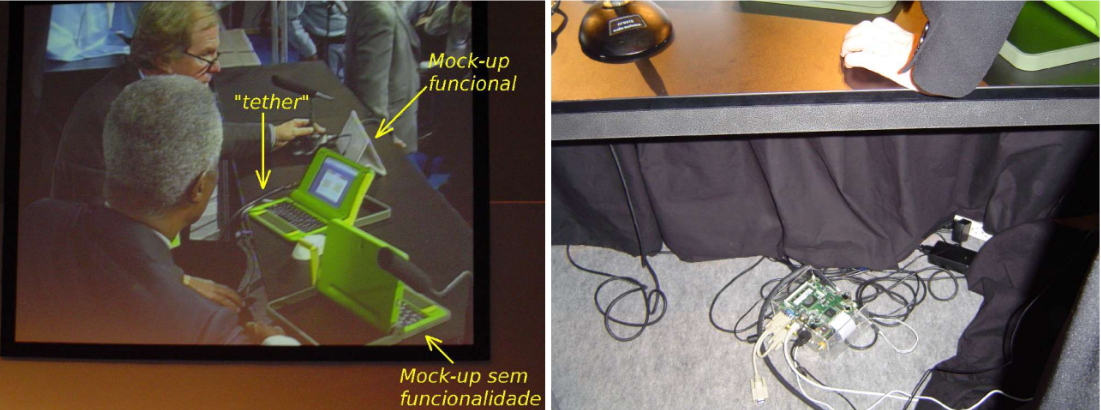
\includegraphics[max size={\textwidth}{\textheight}]{../../imagens/embaixo-mesa.png}

	\end{center}

	\caption{\label{009ca00e74581d7c5448a43112358cb91a959b69}Foto tirada por Victor Mammana mostrando que o OLPC ainda n\~ao tinha um prot\'otipo completo, mesmo com as negocia\c{c}\~oes avan\c{c}adas com o Governo Brasileiro. Essa situa\c{c}\~ao gerou muita inseguran\c{c}a na Presid\^encia da Rep\'ublica. (cr\'editos: Victor Mammana)}

\end{figure}

Sobre essa situa\c{c}\~ao,  MAMMANA (2006) alertava:













\noindent\begin{center}\mbox{\centering\fbox{\centering\par\parbox{0.7\linewidth}{\small\textit{\textquotedbl\{\}Do ponto de vista t\'ecnico, \'e preciso estar atento \`as cr\'{\i}ticas referentes \`a maneira desestruturada com que v\^em sendo proposto, gerando preocupa\c{c}\~oes sobre sua viabilidade pedag\'ogica, industrial, financeira e social, no longo prazo.\textquotedbl\{\} (Fonte:  MAMMANA (2006))}\normalsize}}}\end{center}


Outro aspecto analisado foi a ergonomia, tendo sido constatado que laptops s\~ao intrinsecamente n\~ao ergon\^omicos, por justapor tela e teclado numa mesma \textquotedbl\{\}caixa\textquotedbl\{\}. Essa constata\c{c}\~ao pode ser sumarizada nesta frase: \textquotedbl\{\}quando a tela est\'a numa posi\c{c}\~ao adequada para os olhos, o teclado fica em posi\c{c}\~ao inadequada, e vice-versa\textquotedbl\{\} (HIRAGA et al., 2006).












Sobre isso,  HIRAGA et al. (2006) constatava:













\noindent\begin{center}\mbox{\centering\fbox{\centering\par\parbox{0.7\linewidth}{\small\textit{\textquotedbl\{\}Ficou evidente que o projeto OLPC n\~ao leva em conta aspectos importantes de ergonomia quanto ao uso saud\'avel do laptop como, por exemplo, a postura corporal do usu\'ario, o tempo de uso, o mobili\'ario a ser utilizado, entre outros.\textquotedbl\{\} (Fonte:  HIRAGA et al. (2006))}\normalsize}}}\end{center}


Ao longo das an\'alises presentes nas dezenas de relat\'orios de avalia\c{c}\~ao gerados, muitas outras quest\~oes criaram questionamentos cujas respostas n\~ao pareciam satisfat\'orias, a exemplo de:













\begin{alineas}
\item obsolesc\^encia dos equipamentos e descarte seguro de lixo-eletr\^onico;
\item custo de aquisi\c{c}\~ao para o governo brasileiro;
\item manuten\c{c}\~ao dos equipamentos;
\item garantia de acesso \`a internet no prazo necess\'ario;
\item seguran\c{c}a das crian\c{c}as em v\'arios aspectos (e.g. conte\'udos impr\'oprios, exposi\c{c}\~ao a situa\c{c}\~oes de risco nas redes sociais);
\item capacita\c{c}\~ao dos profissionais de educa\c{c}\~ao para promover a melhor utiliza\c{c}\~ao dos equipamentos; e
\item custo da infraestrutura perif\'erica (adequa\c{c}\~ao do mobili\'ario, sistemas de carregamento de baterias, entre outros).
\end{alineas}

Em suma, o que se constatou \'e que, pelas dimens\~oes do Brasil e os prazos ex\'{\i}guos de ades\~ao exigidos pelo OLPC, havia muitos riscos para o sistema educacional brasileiro. Por outro lado, para pa\'{\i}ses menores, a ades\~ao poderia fazer mais sentido, dado que essas quest\~oes poderiam ser tratadas com mais detalhe e controle.












N\~ao obstante todas estas d\'uvidas, o valor da proposta OLPC foi reconhecido. \'E poss\'{\i}vel identificar na documenta\c{c}\~ao existente a \^ansia dos pesquisadores envolvidos em encontrar uma alternativa que fosse mais adequada \`a realidade brasileira, mas que, ao mesmo tempo, permanecesse usufruindo das virtudes pedag\'ogicas da proposta de Papert, sem os desafios or\c{c}ament\'arios, industriais e log\'{\i}sticos da forma de implanta\c{c}\~ao decorrente da proposta de Negroponte.












\subsection[A avalia\c{c}\~ao do PID pelo CTI como g\^enese do WASH]{A avalia\c{c}\~ao do PID pelo CTI como g\^enese do WASH}\label{A avalia\c{c}\~ao do PID pelo CTI como g\^enese do WASH}
Feitas essas reflex\~oes sobre o OLPC, cabe discorrer sobre um outro elemento importante para a concep\c{c}\~ao do WASH: a avalia\c{c}\~ao do Programa de Inclus\~ao Digital (PID), do Minist\'erio da Ci\^encia e Tecnologia (MCT), que era conduzido pela Secretaria de Inclus\~ao Social, nos anos, de 2005 a 2009. A avalia\c{c}\~ao, por seu lado, foi conduzida pelo Centro de Tecnologia da Informa\c{c}\~ao Renato Archer, em 2009-2010, coordenada pelo Dr. Victor Mammana, quando era chefe divis\~ao daquela unidade de pesquisa.












O PID, do Minist\'erio da Ci\^encia e Tecnologia (MCTI), na primeira d\'ecada do s\'eculo era fundamentado na disponibiliza\c{c}\~ao de infraestrutura, na forma de telecentros, carecendo de uma vis\~ao mais estruturada e sem previs\~ao de investimento nos verdadeiros atores do processo: as pessoas (CGEE, 2010). A maior parte do investimento era voltada para constru\c{c}\~ao de edifica\c{c}\~oes e aquisi\c{c}\~ao de equipamentos.












A avalia\c{c}\~ao do PID, solicitada pela pr\'opria SECIS, como elemento de qualifica\c{c}\~ao de suas pol\'{\i}ticas, foi conduzida pelo CTI, no contexto de um contrato com o Centro de Gest\~ao e Estudos Estrat\'egicos (CGEE) do MCT. Pudemos constatar que esse trabalho de avalia\c{c}\~ao foi o grande marco para a concep\c{c}\~ao do WASH, quando as respostas para os questionamentos levantados no OLPC come\c{c}aram a encontrar uma solu\c{c}\~ao. \'E da avalia\c{c}\~ao do PID que surgem, pela primeira vez, alguns elementos que hoje est\~ao presentes na Portaria CTI 178/2018.












O PID era um Programa baseado em recursos de emendas parlamentares, direcionadas para implementar telecentros por todo o pa\'{\i}s. Os recursos eram repassados para a SECIS, que gerenciava a cria\c{c}\~ao dos telecentros nas cidades interessadas, com fiscaliza\c{c}\~ao e apoio t\'ecnico da Caixa Econ\^omica. Cerca de 150 milh\~oes de reais foram empregados em cinco anos, em projetos de inclus\~ao social e digital (CGEE, 2010), colocando a iniciativa em patamar equivalente ao do Proinfo, para o mesmo per\'{\i}odo. O formato era particularmente atraente para os parlamentares, que podiam destinar o investimento para suas bases eleitorais. Isso inaugurou um inusitado interesse dos parlamentares pelo Minist\'erio da Ci\^encia e Tecnologia. Da parte do Minist\'erio, a condu\c{c}\~ao t\'ecnica de servidores da pasta e a fiscaliza\c{c}\~ao da Caixa Econ\^omica garantiam a devida \textquotedbl\{\}pasteuriza\c{c}\~ao\textquotedbl\{\} de interesses meramente pol\'{\i}ticos.












Os telecentros, no contexto do PID, eram estruturas f\'{\i}sicas (pr\'edios), equipados com computadores e conectividade (muitas vezes viabilizada pelo GESAC), com vistas a oferecer acesso \`a internet para os cidad\~aos da regi\~ao.












Sobre isso, os autores da avalia\c{c}\~ao CGEE (2010) identificaram, com base nos documentos constitutivos do PID, o tipo de equipamento p\'ublico que se pretendia construir no Programa antes de 2008:













\noindent\begin{center}\mbox{\centering\fbox{\centering\par\parbox{0.7\linewidth}{\small\textit{\textquotedbl\{\}(...) edifica\c{c}\~ao sob mando de uma institui\c{c}\~ao local, edifica\c{c}\~ao esta que, oficialmente: pode sofrer reformas, receber computadores conectados \`a internet, devendo estar aberta ao p\'ublico e oferecer acessibilidade f\'{\i}sica. A edifica\c{c}\~ao pode conter corpo de apoio, que por sua vez pode receber uma \'unica rodada de capacita\c{c}\~ao\textquotedbl\{\} (Fonte: CGEE (2010))}\normalsize}}}\end{center}


Esta descri\c{c}\~ao, por si s\'o, transparece a exist\^encia de fragilidades no Programa PID, na sua concep\c{c}\~ao original, como ficou bastante evidente na manifesta\c{c}\~ao dos avaliadores do CTI:













\noindent\begin{center}\mbox{\centering\fbox{\centering\par\parbox{0.7\linewidth}{\small\textit{\textquotedbl\{\}(...) o resultado pretendido (do PID) se omite quando n\~ao orienta o gestor local sobre op\c{c}\~oes de arranjo institucional para o centro/unidade, quando n\~ao prepara o sistema para a avalia\c{c}\~ao continuada, quando tangencia a quest\~ao educacional e se satisfaz com uma rela\c{c}\~ao com a municipalidade limitada ao tempo de implanta\c{c}\~ao do projeto, sem criar mecanismos para perpetuar esta intera\c{c}\~ao\textquotedbl\{\} (Fonte: CGEE (2010))}\normalsize}}}\end{center}


Foi da an\'alise das defici\^encias do OLPC e do PID, com influ\^encias do trabalho de Afira Ripper, que o Programa WASH nasceu, com ideias cujo amadurecimento se consolidaram em 2009-2010, quando o relat\'orio final de avalia\c{c}\~ao do PID foi entregue  (CGEE, 2010). Naquele relat\'orio apresentado ao CGEE, surge na forma de recomenda\c{c}\~ao para a revis\~ao do PID, os elementos que depois seriam a base do WASH, registrados tamb\'em na Portaria CTI 178/2018. Textualmente, consta o seguinte em  CGEE (2010):













\noindent\begin{center}\mbox{\centering\fbox{\centering\par\parbox{0.7\linewidth}{\small\textit{\textquotedbl\{\}A SECIS poderia, em conjunto com o CNPq, criar bolsas semelhantes \`as existentes para promo\c{c}\~ao da excel\^encia da doc\^encia (e.g. PQ e DT), mas no caso voltadas para motivar a participa\c{c}\~ao \`a dist\^ancia de membros da academia nos projetos do PIDS. Esta participa\c{c}\~ao poderia se dar de diversas formas como, por exemplo, pela orienta\c{c}\~ao de alunos de inicia\c{c}\~ao cient\'{\i}fica atuantes dentro dos centros/unidades, ou mesmo pela verifica\c{c}\~ao dos procedimentos pedag\'ogicos, proposi\c{c}\~ao de melhorias, elabora\c{c}\~ao de relat\'orios, verifica\c{c}\~ao de resultados etc. Este membro da academia, com caracter\'{\i}sticas de um “tutor”, se transformaria num agente da SECIS e elo entre ela e a “ponta”. A atua\c{c}\~ao deste agente poderia se dar no contexto de suas atividades acad\^emicas, dentro da universidade em que estivesse sediado.\textquotedbl\{\} (Fonte:  CGEE (2010))}\normalsize}}}\end{center}


O texto acima foi produzido quatro anos antes do primeiro evento do WASH (2013), antecipando parcialmente as caracter\'{\i}sticas que posteriormente estariam presentes na Portaria CTI 178/2018, quase uma d\'ecada depois. Este registro mostra que a proposta do WASH tem base num aprendizado muito longo sobre pol\'{\i}ticas p\'ublicas de educa\c{c}\~ao (OLPC), de inclus\~ao (PID) e de governo eletr\^onico (GESAC), embasando-se em fontes seguras e robustas.












\subsection[Papert no Brasil pela \'otica de Afira Ripper]{Papert no Brasil pela \'otica de Afira Ripper}\label{Papert no Brasil pela \'otica de Afira Ripper}
Nesta se\c{c}\~ao, trazemos uma vis\~ao sobre como Papert se aproximou do Brasil na d\'ecada de 70, a qual nem sempre est\'a presente na literatura sobre o assunto. Para isso, usamos como fonte a entrevista realizada por esta autora com a Profa. Dra. Afira Vianna Ripper, que foi testemunha ocular do que aconteceu naquele per\'{\i}odo. Sua entrevista \'e um dos produtos educacionais desta disserta\c{c}\~ao, e contou com a contribui\c{c}\~ao de Will Namen, Denise Vieira Pereira e Angel Luis. Um esmerado trabalho de produ\c{c}\~ao coordenado, foi realizado, observando os preceitos da acessibilidade. Como resultado, o v\'{\i}deo da entrevista conta com tradu\c{c}\~ao em libras, realizada pela int\'erprete Juliana Moralles Louvison. Esta entrevista consta do Cap\'{\i}tulo de Produtos Educacionais.












Professora da Pedagogia da Unicamp, desde a d\'ecada de 70, atualmente aposentada, Afira \'e uma figura que esteve presente em v\'arios momentos impactantes para a hist\'oria que se registra aqui. Sobressai o papel pioneiro que  desempenhou na cidade de Campinas na d\'ecada de 80, quando levou, em car\'ater piloto, pr\'aticas de Papert para escolas p\'ublicas municipais. Ela inaugurou o emprego de Bolsas da FAPESP (Funda\c{c}\~ao Paulista equivalente ao CNPq), direcionadas a professores do ensino fundamental participantes do projeto, uma abordagem que guarda certa similitude com o que foi implementado no WASH, no caso de Bolsas de Extens\~ao do CNPq. O coordenador do WASH, reconhece a influ\^encia desse projeto na concep\c{c}\~ao do Programa WASH.












Outro momento em que as hist\'orias se cruzaram foi a participa\c{c}\~ao de Afira Ripper na avalia\c{c}\~ao do OLPC em 2006, convidada pelo atual coordenador do WASH, que na \'epoca coordenava a avalia\c{c}\~ao por parte do CTI. Naquele epis\'odio, segundo relato do coordenador do WASH, ele reencontrou muitos daqueles que interagira no MIT, a exemplo de David Cavallo, entre outros. Ali\'as, seu esposo esteve presente em atividades do Centre Mondial Informatique et Ressource Humaine, na d\'ecada de 80, onde Negroponte atuou como diretor.












Como se ver\'a ao longo deste texto, Afira foi uma observadora brasileira privilegiada no que se refere \`as contribui\c{c}\~oes de Papert, e n\~ao \'e exagero dizer que a chegada relativamente precoce da \textquotedbl\{\}filosofia\textquotedbl\{\} LOGO no Brasil teve grande contribui\c{c}\~ao dela.












Afira havia se transferido para os Estados Unidos no come\c{c}o da d\'ecada de 60 para acompanhar seu esposo, o Prof. Jos\'e Ellis Ripper Filho, em seu doutorado no MIT.












Inquieta e comprometida com sua carreira, n\~ao era seu perfil permanecer apenas como acompanhante do esposo e buscou uma atividade no seu campo de forma\c{c}\~ao. Foi assim que se engajou como aluna ouvinte no MIT, tendo sido estudante e, depois, tendo convivido profissionalmente com Papert, em 1973. A experi\^encia foi bastante marcante para ela, tendo impacto tamb\'em na sua vida pessoal, dado que seu filho foi a primeira crian\c{c}a brasileira a experimentar a linguagem LOGO, quando estava sendo instalado o Media Lab, no MIT.












A professora Afira retornou ao Brasil e foi trabalhar num projeto de matem\'atica junto com o professor Ubiratan D’ambr\'osio, diretor do Instituto de Matem\'atica da Unicamp, IMEC, no come\c{c}o da d\'ecada de 70. A experi\^encia anterior de Afira no grupo de Papert oportunizou o convite, pela Unicamp, para que Seymour Papert, da \'area de educa\c{c}\~ao, e Marvin Minsky, da \'area de intelig\^encia artificial, viessem ao Brasil.












Antes de prosseguir, \'e preciso abrir um par\^enteses sobre como a Profa. Afira Ripper optou pela Unicamp, em seu retorno ao Brasil.  MAMMANA (2018), ap\'os entrevista com Prof. Jos\'e Ellis Ripper Filho, esposo da Profa. Afira, traz um relato interessante sobre a decis\~ao dos pesquisadores brasileiros, expatriados nos Estados Unidos na d\'ecada de 60, de retornarem ao Brasil em plena ditadura. Em resumo, a escolha de Campinas foi decorrente da invas\~ao da UNB pelo Ex\'ercito em 1968. Bras\'{\i}lia era o destino preferido dos pesquisadores Brasileiros, por conta da proposta arrojada de Darcy Ribeiro para a UNB, mas ponderaram o risco de estarem pr\'oximos demais da \textquotedbl\{\}toca do le\~ao\textquotedbl\{\}  (MAMMANA, 2018), optando pela Unicamp. Essa decis\~ao dos pesquisadores foi determinante para a consolida\c{c}\~ao da UNICAMP e, consequentemente, para a voca\c{c}\~ao de Campinas em ci\^encia e tecnologia, que se observou nas d\'ecadas subsequentes.












Cabe registrar que o papel de Ubiratan D Ambr\'osio \'e relatado, tamb\'em, por ALVAREZ (2015), mas a nuance do papel da Profa. Afira Ripper n\~ao \'e relatada.












Ali\'as, h\'a ainda que se uniformizar as fontes hist\'oricas para identificar o papel de cada institui\c{c}\~ao brasileira, nesse per\'{\i}odo. Por exemplo,  ALVAREZ (2015) menciona o pioneirismo da Universidade Federal do Rio de Janeiro, 1966, no uso de computador em atividades acad\^emicas. Por outro lado, o ITA reinvindica a constru\c{c}\~ao do primeiro computador em 1963, constru\'{\i}do no contexto de um curso de gradua\c{c}\~ao, com a participa\c{c}\~ao do, ent\~ao, estudante Jos\'e Ellis Ripper Filho.












Naquele tempo, d\'ecada de 70, a intelig\^encia artificial era uma disciplina extremamente nova. Os pesquisadores do MIT vieram para passar um m\^es dando palestras no IMEC da UNICAMP, sobre o programa, de intelig\^encia artificial e sobre a linguagem LOGO, que ainda estava numa fase inicial mesmo nos Estados Unidos. Afira relata que a primeira medida tomada pelos professores da Unicamp foi traduzir o livro do Papert sobre a linguagem LOGO.












Os professores brasileiros j\'a estavam contaminados pela ideia de que o trabalho com o computador poderia empoderar as crian\c{c}as em rela\c{c}\~ao ao exerc\'{\i}cio dos racioc\'{\i}nios matem\'atico e l\'ogico. \textquotedbl\{\}Refiro-me ao computador do pr\'e mouse, um computador em que voc\^e digitava os comandos e tinha que apertar o enter \textquotedbl\{\}, diz Afira Ripper sobre a interface de computador existente naquele tempo.












Muitos desenvolvimentos se seguiram depois, at\'e o ponto em que a Profa. Afira Ripper percebeu-se em condi\c{c}\~oes de estabelecer um projeto semelhante ao do MIT, no Brasil.












Afira formulou o Projeto Eureka, que pretendia introduzir o computador na escola como ferramenta pedag\'ogica para o trabalho do professor. O Projeto foi apresentado para a Secretaria Municipal de Educa\c{c}\~ao de Campinas, tendo sido aceito como projeto pedag\'ogico da Secretaria.












Ainda, segundo o relato da Profa. Afira Ripper, posteriormente uma diretora de pr\'e-escola (p\'ublica) de Campinas abarcou o projeto de pesquisa e inicia\c{c}\~ao cient\'{\i}fica, formando as professoras que passariam a trabalhar com os alunos, dentro da filosofia de Montessori. Na interpreta\c{c}\~ao da Profa. Afira, esta abordagem criava uma responsabilidade redobrada para os alunos que, motivados pelo LOGO, fazia com que eles tivessem um interesse enorme pelo computador, mesmo com barreiras iniciais, como a digita\c{c}\~ao, por exemplo.












Em sua entrevista, a professora Afira reporta ter sentido naquela \'epoca muito interesse pelo que os pr\'oprios estudantes conseguiam fazer no computador. Ainda, segundo sua descri\c{c}\~ao, as crian\c{c}as digitavam os c\'odigos e as professoras pediam para que fizessem os gestos dos comandos do LOGO: \textquotedbl\{\}em p\'e\textquotedbl\{\}, \textquotedbl\{\}vire \`a direita\textquotedbl\{\}, \textquotedbl\{\}vire \`a esquerda\textquotedbl\{\}, \textquotedbl\{\}d\^e passos para frente\textquotedbl\{\}, \textquotedbl\{\}para tr\'as\textquotedbl\{\}. Tanto para as crian\c{c}as quanto para os adultos, era um in\'{\i}cio da computa\c{c}\~ao em suas vidas.












Assim, foi poss\'{\i}vel trazer o LOGO como um elemento a mais para levar ao exerc\'{\i}cio natural de conceitos da l\'ogica, da \'algebra, das fun\c{c}\~oes e da teoria de conjuntos, criando um passo-a-passo menos traum\'atico para se chegar a uma experi\^encia mais org\^anica em torno da matem\'atica. Ao mesmo tempo, o LOGO n\~ao se restringe \`a superf\'{\i}cie dos conceitos, permitindo que o pensamento humano experimente ideias bem mais complexas e abstratas, como, por exemplo, a ideia da recurs\~ao, em que algoritmos invocam a si mesmos at\'e os limites da mem\'oria do computador.












Outra pesquisadora do LOGO, no Brasil, foi a professora  Dra Maria Cec\'{\i}lia Baranauskas (Unicamp), que investigou como  se dava a intera\c{c}\~ao de crian\c{c}as com o computador. Para tanto ela ofereceu oficinas para  crian\c{c}as, sendo uma delas Marina de Queiroz Tavares  e, posteriormente, Victor Pellegrini Mammana  tiveram a oportunidade  de  utilizar a Linguagem LOGO em um terminal gr\'afico (GT40), ligado a um mainframe (PDP10), do Centro de Computa\c{c}\~ao da UNICAMP. A disserta\c{c}\~ao de Mestrado de Baranauskas foi sobre os \textquotedbl\{\}Conceitos Geom\'etricos, atrav\'es da Linguagem LOGO\textquotedbl\{\}. A participa\c{c}\~ao da crian\c{c}a Victor naquela \textquotedbl\{\}oficina\textquotedbl\{\} no in\'{\i}cio da d\'ecada de 80, ficou em sua mem\'oria, tendo sido, reconhecidamente por ele, mais uma das inspira\c{c}\~oes para a cria\c{c}\~ao do WASH.












O site do Programa WASH publicou entrevista com a professora Maria Cec\'{\i}lia Baranauskas, na qual ela conta a sua experi\^encia com a Linguagem LOGO e rememora o seu contato com Papert e sua teoria. A entrevista est\'a dispon\'{\i}vel neste link: \textquotedbl\{\}Barreiras entre o homem e o computador e oficinas digitais s\~ao temas com membro da Unesco, Programa WASH\textquotedbl\{\}.












\subsection[A hist\'oria, a pr\'atica, os valores e os conceitos do Programa WASH]{A hist\'oria, a pr\'atica, os valores e os conceitos do Programa WASH}\label{A hist\'oria, a pr\'atica, os valores e os conceitos do Programa WASH}
Nesta se\c{c}\~ao, fazemos uma interpreta\c{c}\~ao do acervo do Programa WASH, principalmente no seu Documento de Refer\^encia, e os relat\'orios apresentados ao CNPq, durante os anos de execu\c{c}\~ao de seus projetos intermedi\'arios  (CNPq, 2020)   (CNPq, 2020a)  (CNPq, 2020b)  (WASHCNPq, 2022). Este esfor\c{c}o visa identificar os valores e conceitos do Programa WASH registrados, desde sua inaugura\c{c}\~ao, em 2013.












Nota-se que, embora tenha sido publicada a portaria em 2018, cinco anos ap\'os o in\'{\i}cio, de suas atividades, o Documento de Refer\^encia busca expressar \textquotedbl\{\}o que o WASH gostaria de ser\textquotedbl\{\}, ao passo que os relat\'orios de execu\c{c}\~ao do Programa entregues ao CNPq, no final de cada projeto, expressam \textquotedbl\{\}aquilo que o WASH conseguiu ser\textquotedbl\{\}.












Como coautora do Documento de Refer\^encia, esta candidata tem credenciais para discorrer sobre sua concep\c{c}\~ao. Esse documento n\~ao foi gerado de cima para baixo, mas constru\'{\i}do a partir de uma pr\'atica cotidiana de experimenta\c{c}\~ao que, com  \textquotedbl\{\}tentativa e erro\textquotedbl\{\}, foi sendo aprimorado pela viv\^encia de cada oficina, de cada projeto de inicia\c{c}\~ao cient\'{\i}fica, de cada roda de conversa, de cada  evento cultural, de cada nova realidade encontrada, das parcerias, das aprendizagens. de cada gera\c{c}\~ao que passou pelo WASH nesses 10 anos. Retrospectivamente, hoje podemos dizer que o processo de cria\c{c}\~ao do WASH seguiu, mesmo que instintivamente, o que o pr\'oprio Papert preconizava: que tentar e errar \'e uma forma de aprender. Portanto, \'e poss\'{\i}vel concluir que o documento de refer\^encia do WASH \'e resultado de um aprendizado de cinco anos de experimenta\c{c}\~ao de pr\'aticas educacionais e culturais.












Segundo consta no relat\'orio CNPq (2020), o Programa WASH foi iniciado em 28 de setembro de 2013, com \textquotedbl\{\}\'unico e pontual evento de hackers\textquotedbl\{\}. Essa informa\c{c}\~ao pode ser confirmada, tamb\'em, na plataforma Platu\'oxe (ver Fig. 27), que tem o registro do evento citado, com 92 participantes, entre adultos, adolescentes e crian\c{c}as. Nesse evento, foram realizadas diversas atividades voltadas para \textquotedbl\{\}hackers\textquotedbl\{\} e \textquotedbl\{\}geeks\textquotedbl\{\}, termos que designam pessoas aficionadas em tecnologia. Dentre as atividades do primeiro evento constavam: oficina de ardu\'{\i}no, oficina linguagem de programa\c{c}\~ao Alice, curso de drone, demonstra\c{c}\~oes de f\'{\i}sica e desafios.














\captionsetup{format=plain}
\begin{figure}[htb]

	\begin{center}

		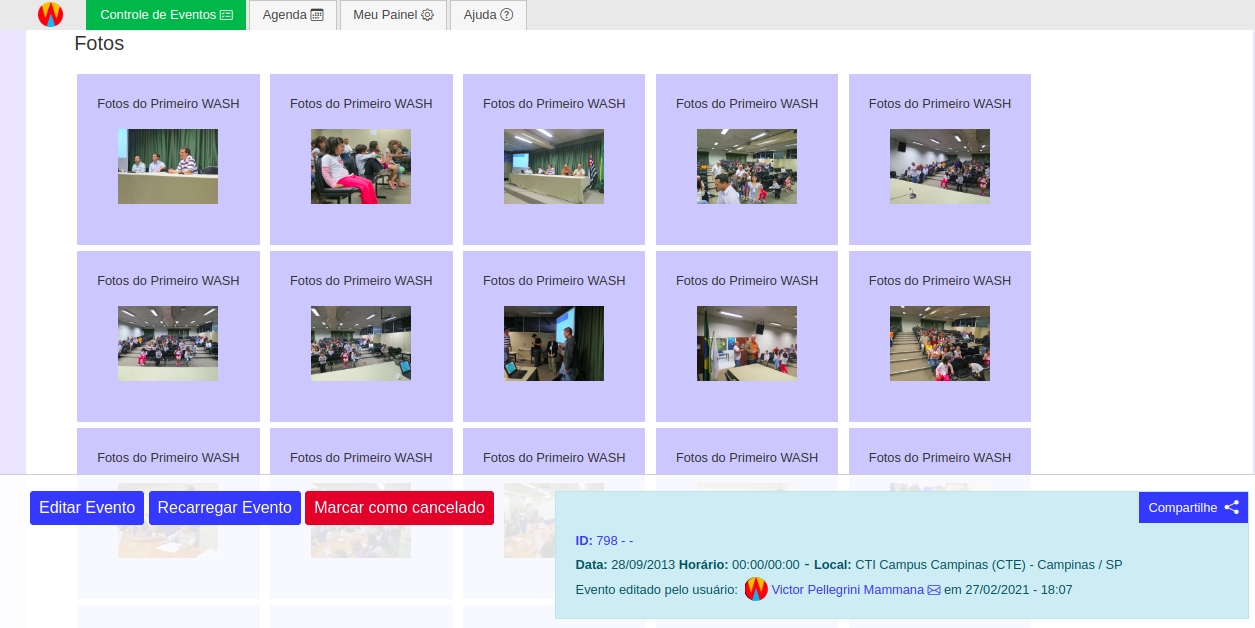
\includegraphics[max size={\textwidth}{\textheight}]{../../imagens/primeiro-wash-corte.png}

	\end{center}

	\caption{\label{11f122f06c11abd40a3af9574514af9c30c712b9}Imagem da tela da plataforma Platu\'oxe, registro do primeiro evento do WASH realizado em 28 de setembro de 2013. (fonte: Plataforma Platu\'oxe)}

\end{figure}

O foco em \textquotedbl\{\}hackers\textquotedbl\{\} (ou \textquotedbl\{\}geeks\textquotedbl\{\}) do primeiro evento indica que o p\'ublico alvo, inicialmente, era constitu\'{\i}do de jovens e adultos, com  poucas crian\c{c}as. Esse fato explica, em parte, o nome do programa, que usou a palavra em portugu\^es \textquotedbl\{\}aficionados\textquotedbl\{\} como tradu\c{c}\~ao livre de \textquotedbl\{\}hackers\textquotedbl\{\} ou \textquotedbl\{\}geeks\textquotedbl\{\}. Por diversas vezes, foi poss\'{\i}vel testemunhar as manifesta\c{c}\~oes do coordenador do WASH lamentando a manuten\c{c}\~ao desse nome para um Programa que depois veio atender crian\c{c}as (informa\c{c}\~ao autorizada pelo coordenador). Entretanto, observamos que o \textquotedbl\{\}batismo\textquotedbl\{\} do Programa fugira ao controle de seus criadores, uma vez que o nome do WASH fora adotado tamb\'em para os eventos com crian\c{c}as que vieram depois, talvez, por sua sonoridade. Assim, \textquotedbl\{\} WASH \textquotedbl\{\} passou a ser a identidade do Programa, mesmo considerando que o acr\^onimo n\~ao reflete com precis\~ao o que tem sido oferecido para os participantes, i.e., STEAM.












Esse fato, por si s\'o, indica que, a rigor, a organiza\c{c}\~ao do primeiro evento n\~ao vislumbrava um programa educacional para a escola p\'ublica.












O caminho em dire\c{c}\~ao a um Programa educacional para a escola p\'ublica foi sendo moldado ao longo de suas re-edi\c{c}\~oes, que gradualmente passaram a atrair um p\'ublico cada vez mais jovem, culminando no encontro definitivo de sua voca\c{c}\~ao, sintetizada em:













\noindent\begin{center}\mbox{\centering\fbox{\centering\par\parbox{0.7\linewidth}{\small\textit{\textquotedbl\{\}educa\c{c}\~ao cient\'{\i}fica e tecnol\'ogica para o ensino fundamental, mediante protagonismo de jovens do ensino m\'edio e superior\textquotedbl\{\} (Fonte:  CNPq (2020))}\normalsize}}}\end{center}


Ambicionando aplicar o que fora aprendido com avalia\c{c}\~ao pedag\'ogica do OLPC, inclusive com a influ\^encia e colabora\c{c}\~ao da professora Dra.Afira Vianna Ripper que, como vimos, participara da referida avalia\c{c}\~ao, o WASH sempre buscou se vincular aos conceitos subjacentes ao pensamento de Papert.












Rapidamente, acompanhando a tend\^encia mundial, o Programa se identificou com o STEM (Science, Technology, Engineering and Mathematics), adotando,tamb\'em, as artes como um elemento fundamental de suas oficinas  (CNPq, 2020), fato que pode ser atribu\'{\i}do \`a influ\^encia do GESAC.1












Como egressa do Programa GESAC, e ainda sem conhecer os conceitos constru\'{\i}dos por outros (e.g.  YAKMAN (2019)), esta autora prop\^os a introdu\c{c}\~ao das artes nas oficinas do WASH, aproximando-as das abordagens STEAM.












Essa mudan\c{c}a de \textquotedbl\{\}evento de hackers\textquotedbl\{\} para \textquotedbl\{\}evento STEAM\textquotedbl\{\} levou algum tempo para amadurecer e exigiu um compromisso maior com o conceito de m\'etodo cient\'{\i}fico, requerendo do Programa a ado\c{c}\~ao de um \textquotedbl\{\}crit\'erio de demarca\c{c}\~ao\textquotedbl\{\} da ci\^encia.












 CHIBENI (2006) alerta para o fato de que \textquotedbl\{\}n\~ao h\'a um m\'etodo cient\'{\i}fico no sentido de uma receita universal para se fazer ci\^encia\textquotedbl\{\}, mas \'e poss\'{\i}vel identificar na ci\^encia algumas especificidades em rela\c{c}\~ao a outras formas de adquirir saber.












Os criadores do WASH, em v\'arios pontos da documenta\c{c}\~ao existente, mencionavam, inicialmente, o crit\'erio da falseabilidade de Popper como forma de verificar se uma proposi\c{c}\~ao era cient\'{\i}fica ou n\~ao e; portanto, pass\'{\i}vel de fazer parte das atividades do Programa. Para isso, apresentavam a seguinte defini\c{c}\~ao como sendo uma \textquotedbl\{\}forma simplificada de expressar o pensamento de Popper\textquotedbl\{\}  (CNPq, 2020):













\noindent\begin{center}\mbox{\centering\fbox{\centering\par\parbox{0.7\linewidth}{\small\textit{\textquotedbl\{\}Falseabilidade - Todo conhecimento cient\'{\i}fico pode ser questionado e contestado, quando pode ser requerida a revis\~ao de suas bases experimentais e te\'oricas. O conhecimento que n\~ao pode ser contestado, a exemplo da f\'e religiosa ou do ocultismo, n\~ao \'e um conhecimento cient\'{\i}fico.\textquotedbl\{\}  (CNPq, 2020).}\normalsize}}}\end{center}


\'E poss\'{\i}vel identificar na documenta\c{c}\~ao do WASH o reconhecimento de que o crit\'erio da falseabilidade foi considerado como um \textquotedbl\{\}ponto de partida\textquotedbl\{\} para o trabalho de \textquotedbl\{\}demarca\c{c}\~ao de ci\^encia e n\~ao-ci\^encia\textquotedbl\{\}, mas que para \textquotedbl\{\}os primeiros anos escolares \'e preciso resistir \`a tenta\c{c}\~ao de ir muito al\'em disso na busca por uma defini\c{c}\~ao \'unica e generalizada do m\'etodo cient\'{\i}fico\textquotedbl\{\}  (CNPq, 2020).












O que se identifica nas pr\'aticas do WASH, seja pela inspe\c{c}\~ao da documenta\c{c}\~ao formal (relat\'orios), quanto pela busca dos temas de oficinas na plataforma \textquotedbl\{\}Platu\'oxe\textquotedbl\{\}, \'e que nunca existiu uma preocupa\c{c}\~ao em definir o conceito de m\'etodo cient\'{\i}fico para as crian\c{c}as, adotando como \textquotedbl\{\}divisa \textquotedbl\{\} a ideia simples de que \textquotedbl\{\}se voc\^e pode questionar, \'e ci\^encia\textquotedbl\{\}  (CNPq, 2020). Esta simplifica\c{c}\~ao est\'a de bom tamanho para os anos escolares iniciais, mas \'e claro que precisa se ampliar, com o amadurecimento.












A intera\c{c}\~ao, o trabalho desenvolvido com o coordenador do Programa WASH, bem como a an\'alise da documenta\c{c}\~ao existente  (CNPq, 2020)  (CNPQ, 2020a)  (MAMMANA et al., 2022a) mostram que existe uma predile\c{c}\~ao por uma defini\c{c}\~ao bastante simples e direta de ci\^encia, que \'e de f\'acil assimila\c{c}\~ao por todos os colaboradores:













\noindent\begin{center}\mbox{\centering\fbox{\centering\par\parbox{0.7\linewidth}{\small\textit{\textquotedbl\{\}Ci\^encia \'e a compreens\~ao que o outro constr\'oi sobre o conhecimento de algu\'em\textquotedbl\{\} (Fonte:   MAMMANA, V.P., CGEE (2010), p\'ag. 48)}\normalsize}}}\end{center}


A frase acima foi primeiramente apresentada em  CGEE (2010), pelo coordenador do Programa WASH, tendo car\'ater original. O conceito subjacente \'e de que \textquotedbl\{\}n\~ao h\'a ci\^encia se n\~ao houver a compreens\~ao por algu\'em dos conhecimentos gerados por outrem, mostrando que a ci\^encia tem car\'ater social, sendo parte integrante da cultura de uma comunidade\textquotedbl\{\}  (CNPq, 2020).












A forma como esse conceito \'e aproveitado no contexto da escola fundamental fica evidente na transcri\c{c}\~ao  CNPq (2020), abaixo:













\noindent\begin{center}\mbox{\centering\fbox{\centering\par\parbox{0.7\linewidth}{\small\textit{\textquotedbl\{\}Na atua\c{c}\~ao do WASH junto aos primeiros anos escolares, h\'a uma preocupa\c{c}\~ao de estimular uma boa comunica\c{c}\~ao, seja atrav\'es da prepara\c{c}\~ao dos bolsistas para a multiplica\c{c}\~ao (oficinas), registro de resultados ou produ\c{c}\~ao de audiovisual, por exemplo. Em outras palavras, \'e a preocupa\c{c}\~ao com a capacidade de produzir narrativas calcadas num m\'etodo.\textquotedbl\{\} (Fonte:  CNPq (2020))}\normalsize}}}\end{center}


Este est\'{\i}mulo \`a produ\c{c}\~ao de narrativas, que facilitem a compreens\~ao de algum conhecimento \'e, em \'ultima an\'alise, o m\'etodo cient\'{\i}fico do WASH. Atrav\'es dele, a crian\c{c}a (ou jovem) \'e convidada a organizar o conhecimento adquirido, para que, atrav\'es da convers\~ao em um discurso, outros possam assimil\'a-lo e question\'a-lo. Esta abordagem fica bem clara em  WASH CNPq (2022):













\noindent\begin{center}\mbox{\centering\fbox{\centering\par\parbox{0.7\linewidth}{\small\textit{\textquotedbl\{\}(...) Outra atividade oferecida pelo WASH \'e a constru\c{c}\~ao de discursos pelos participantes, muitas vezes na dire\c{c}\~ao de uma produ\c{c}\~ao audiovisual como ferramenta para o exerc\'{\i}cio de comunica\c{c}\~ao de suas descobertas e aprendizados. Nesse processo, s\~ao estimulados o planejamento, o debate de ideias, o trabalho em coopera\c{c}\~ao, a organiza\c{c}\~ao e algumas t\'ecnicas de produ\c{c}\~ao audiovisual, embora este \'ultimo aspecto seja mais instrumental. Tudo isso \'e feito de forma l\'udica e dentro da zona proximal da crian\c{c}a.\textquotedbl\{\} (Fonte:  WASH CNPq (2022))}\normalsize}}}\end{center}


Al\'em da quest\~ao de dissemina\c{c}\~ao do m\'etodo cient\'{\i}fico para a escola p\'ublica, \'e poss\'{\i}vel identificar outras preocupa\c{c}\~oes que levaram \`a formula\c{c}\~ao do WASH.












Na Fundamenta\c{c}\~ao Te\'orica, mostramos a discrep\^ancia entre o investimento por hora, por aluno, no \^ambito da escola p\'ublica em rela\c{c}\~ao \`a escola privada (ver tabela 1). Este investimento mostra-se de 4 a 5 vezes maior para crian\c{c}as matriculadas em escolas privadas de m\'edio padr\~ao em rela\c{c}\~ao \`a escola p\'ublica, podendo chegar a 10 vezes mais para escolas privadas de alto padr\~ao.












A situa\c{c}\~ao fica mais cr\'{\i}tica quando se consideram as oportunidades criadas pelas atividades de contraturno  (CNPq, 2020b):













\noindent\begin{center}\mbox{\centering\fbox{\centering\par\parbox{0.7\linewidth}{\small\textit{\textquotedbl\{\}Alunos de escolas privadas tradicionais da cidade de S\~ao Paulo, por exemplo, chegam a ter v\'arias dezenas de op\c{c}\~oes de atividades de contraturno que permitem enriquecer sua forma\c{c}\~ao em \'areas variadas, tais como: l\'{\i}nguas estrangeiras, programa\c{c}\~ao de computadores, Cultura Maker, STEAM, programa\c{c}\~ao de jogos de computador, artes pl\'asticas, m\'usica, modalidades esportivas, dan\c{c}a, express\~ao corporal, entre outras. Esta disparidade afeta principalmente os alunos de escolas p\'ublicas em regi\~oes perif\'ericas, que t\^em menos op\c{c}\~oes ainda para complementar sua forma\c{c}\~ao.\textquotedbl\{\} (Fonte:  CNPq (2020b))}\normalsize}}}\end{center}


Na releitura do Documento de Refer\^encia do WASH, da qual esta que escreve \'e coautora, observamos que a preocupa\c{c}\~ao em enfrentar essa disparidade sempre esteve presente no Programa. Em  CNPq (2020b), \'e identificada, por exemplo, a preocupa\c{c}\~ao com o in\'{\i}cio prematuro da vida profissional dos estudantes da escola p\'ublica, que acabam por interromper seus estudos, aprofundando o fosso em rela\c{c}\~ao \`as oportunidades das crian\c{c}as de fam\'{\i}lias abastadas. Na mesma refer\^encia, \'e enfatizada a jornada de trabalho dom\'estico antecipada  das meninas, bem como dos cuidados com irm\~aos e irm\~as menores, dificultando ainda mais o acesso, para as meninas, \`as mesmas oportunidades dispon\'{\i}veis aos estudantes do sexo masculino na mesma condi\c{c}\~ao social.












Portanto, fica evidente a preocupa\c{c}\~ao dos criadores do WASH com a \textquotedbl\{\} injusta diferen\c{c}a \textquotedbl\{\} existente entre estudantes de escolas p\'ublicas e privadas, que pode ter consequ\^encias duradouras para a inser\c{c}\~ao daquele indiv\'{\i}duo em sua pr\'opria cultura, prejudicando seu desempenho como cidad\~ao ativo e pr\'ospero da sociedade\textquotedbl\{\}  (CNPq, 2020b).













\noindent\begin{center}\mbox{\centering\fbox{\centering\par\parbox{0.7\linewidth}{\small\textit{\textquotedbl\{\}A principal contribui\c{c}\~ao que o Programa WASH busca dar \'e a constru\c{c}\~ao de uma forma escal\'avel para levar o STEAM \`a escola p\'ublica brasileira, respeitando suas peculiaridades, suas miss\~oes pedag\'ogicas e seus valores culturais.\textquotedbl\{\} (Fonte:  CNPq (2020))}\normalsize}}}\end{center}


O estudo das caracter\'{\i}sticas do Programa WASH, por meio da documenta\c{c}\~ao existente mostra, tamb\'em, a preocupa\c{c}\~ao de seus formuladores em conceb\^e-lo de forma sustent\'avel economicamente, visando valores por hora por aluno compat\'{\i}veis com a capacidade de investimento do setor p\'ublico  (CNPq, 2020b). Em v\'arias ocasi\~oes, o coordenador do WASH revelou que a cria\c{c}\~ao da Plataforma Platu\'oxe teve como motiva\c{c}\~ao principal a caracteriza\c{c}\~ao do custo por hora e por aluno.












Em termos pr\'aticos  (CNPq, 2020), o WASH vem buscando as seguinte caracter\'{\i}sticas para viabilizar a sua dissemina\c{c}\~ao no sistema educacional brasileiro, sem a necessidade de vultuosos investimentos:













\begin{alineas}
\item \textquotedbl\{\}foco no investimento em pessoas e n\~ao em equipamentos, buscando aproveitar a infraestrutura existente;\textquotedbl\{\}
\item \textquotedbl\{\}busca por capilaridade, aproveitando a rede federal de ensino como elemento de regionaliza\c{c}\~ao do programa;\textquotedbl\{\}
\item \textquotedbl\{\}envolvimento de jovens estudantes como elementos de multiplica\c{c}\~ao, desenvolvendo o conceito do ensinar como pretexto para aprender;\textquotedbl\{\}
\item \textquotedbl\{\}uso de meios institucionais j\'a existentes para a viabiliza\c{c}\~ao do financiamento do Programa, a exemplo da pol\'{\i}tica de bolsas do CNPq, a indica\c{c}\~ao de emendas parlamentares diminuindo custos de gest\~ao pela equipe;\textquotedbl\{\}
\item \textquotedbl\{\}cria\c{c}\~ao de uma  \textquotedbl\{\}liturgia pedag\'ogica,\textquotedbl\{\} a partir de viv\^encia, que permita sua reprodu\c{c}\~ao nas v\'arias localidades,sua adapta\c{c}\~ao \`as diferentes realidades em cada regi\~ao;\textquotedbl\{\}
\item \textquotedbl\{\}ren\'uncia ao conceito de curso;\textquotedbl\{\}
\item \textquotedbl\{\}ren\'uncia ao conteudismo, oferta de pelo menos tr\^es atividades motivacionais que podem, ou n\~ao, serem adotadas localmente\textquotedbl\{\}. Estas tr\^es etapas citadas em  CNPq (2020) referem-se \`as tr\^es oficinas de programa\c{c}\~ao mais comuns do WASH: \textquotedbl\{\}Labirinto I\textquotedbl\{\}, \textquotedbl\{\}Labirinto II\textquotedbl\{\} e \textquotedbl\{\}Space Invaders\textquotedbl\{\};
\item \textquotedbl\{\}demonstra\c{c}\~ao de oficinas\textquotedbl\{\} como meio de capacita\c{c}\~ao dos multiplicadores, sempre com foco na
simplicidade de reprodu\c{c}\~ao;\textquotedbl\{\}
\item \textquotedbl\{\}defini\c{c}\~ao clara dos objetivos de cada viv\^encia, sem exig\^encia de pr\'e-requisitos para a participa\c{c}\~ao nas mesmas;\textquotedbl\{\}e
\item \textquotedbl\{\}est\'{\i}mulo para que as viv\^encias encapsulem todo o conhecimento necess\'ario para  atingir  seus objetivos, sempre que poss\'{\i}vel, de forma que o programa possa acolher todas as crian\c{c}as, mesmo aquelas que n\~ao tiveram oportunidade de participar das experi\^encias anteriores.\textquotedbl\{\}
\end{alineas}

Para que essas caracter\'{\i}sticas pudessem ser conquistadas dentro de um patamar de investimentos p\'ublicos vi\'avel, sem a cria\c{c}\~ao de novas estruturas institucionais, os formuladores do WASH conceberam meios para aproveitar o investimento j\'a feito em centros de excel\^encia de pesquisa e educa\c{c}\~ao, existentes no Brasil.












Inicialmente, pela pr\'opria origem profissional do coordenador do WASH, concebeu-se a ideia de estabelecer pontes diretas entre as Unidades de Pesquisa do Minist\'erio de Ci\^encia e Tecnologia e o ensino fundamental.












Nos prim\'ordios do Programa, essa ideia n\~ao fora bem recebida, por alguns servidores do CTI Renato Archer, primeira institui\c{c}\~ao em que oficinas do WASH foram realizadas. Havia um receio de que tal atividade pudesse \textquotedbl\{\} desvirtuar \textquotedbl\{\} a miss\~ao de unidades que tinham a pesquisa como mote principal. Por envolver moradores de bairros de baixa renda, do entorno do CTI Renato Archer, percebia-se algum desconforto com a abertura da institui\c{c}\~ao para a comunidade nos finais de semana, para a realiza\c{c}\~ao das oficinas.












Para os cr\'{\i}ticos da ideia de receber crian\c{c}as em unidades de pesquisa do Minist\'erio, o coordenador do WASH, frequentemente, repetia um relato (testemunhado por esta autora) sobre sua experi\^encia no Lawrence Berkeley Laboratory, na Calif\'ornia, onde realizou a parte de pesquisa de seu trabalho de tese de doutorado:













\noindent\begin{center}\mbox{\centering\fbox{\centering\par\parbox{0.7\linewidth}{\small\textit{\textquotedbl\{\}Quando eu estava no Lawrence Berkeley Lab (LBL) eu me espantava com a presen\c{c}a de crian\c{c}as circulando num instituto t\~ao reputado e s\'erio, com 13 pr\^emios Nobel. O LBL abria suas portas para eventos de educa\c{c}\~ao cient\'{\i}fica para crian\c{c}as de variadas idades. No CTI Renato Archer n\~ao receb\'{\i}amos crian\c{c}as. Talvez, esteja nos faltando receb\^e-las para conquistar  um pr\^emio Nobel para o Brasil.\textquotedbl\{\} (fonte: interpreta\c{c}\~ao autorizada de relato feito pelo coordenador do WASH em suas palestras).}\normalsize}}}\end{center}


Posteriormente, a este in\'{\i}cio restrito ao CTI Renato Archer, o WASH foi sendo levado para outros centros de excel\^encia, tendo havido interesse imediato por parte do Instituto Federal de Educa\c{c}\~ao, Ci\^encia e Tecnologia de S\~ao Paulo-IFSP Campus Campinas.












A Fig. 28, obtida de uma apresenta\c{c}\~ao do WASH de 2016, mostra um diagrama de como a ponte entre o ensino fundamental e os centros de excel\^encia foi imaginada na fase inicial do Programa. Essa concep\c{c}\~ao est\'a presente at\'e os dias de hoje e foi cristalizada no Documento de Refer\^encia anexo \`a Portaria CTI 178/2018.














\captionsetup{format=plain}
\begin{figure}[htb]

	\begin{center}

		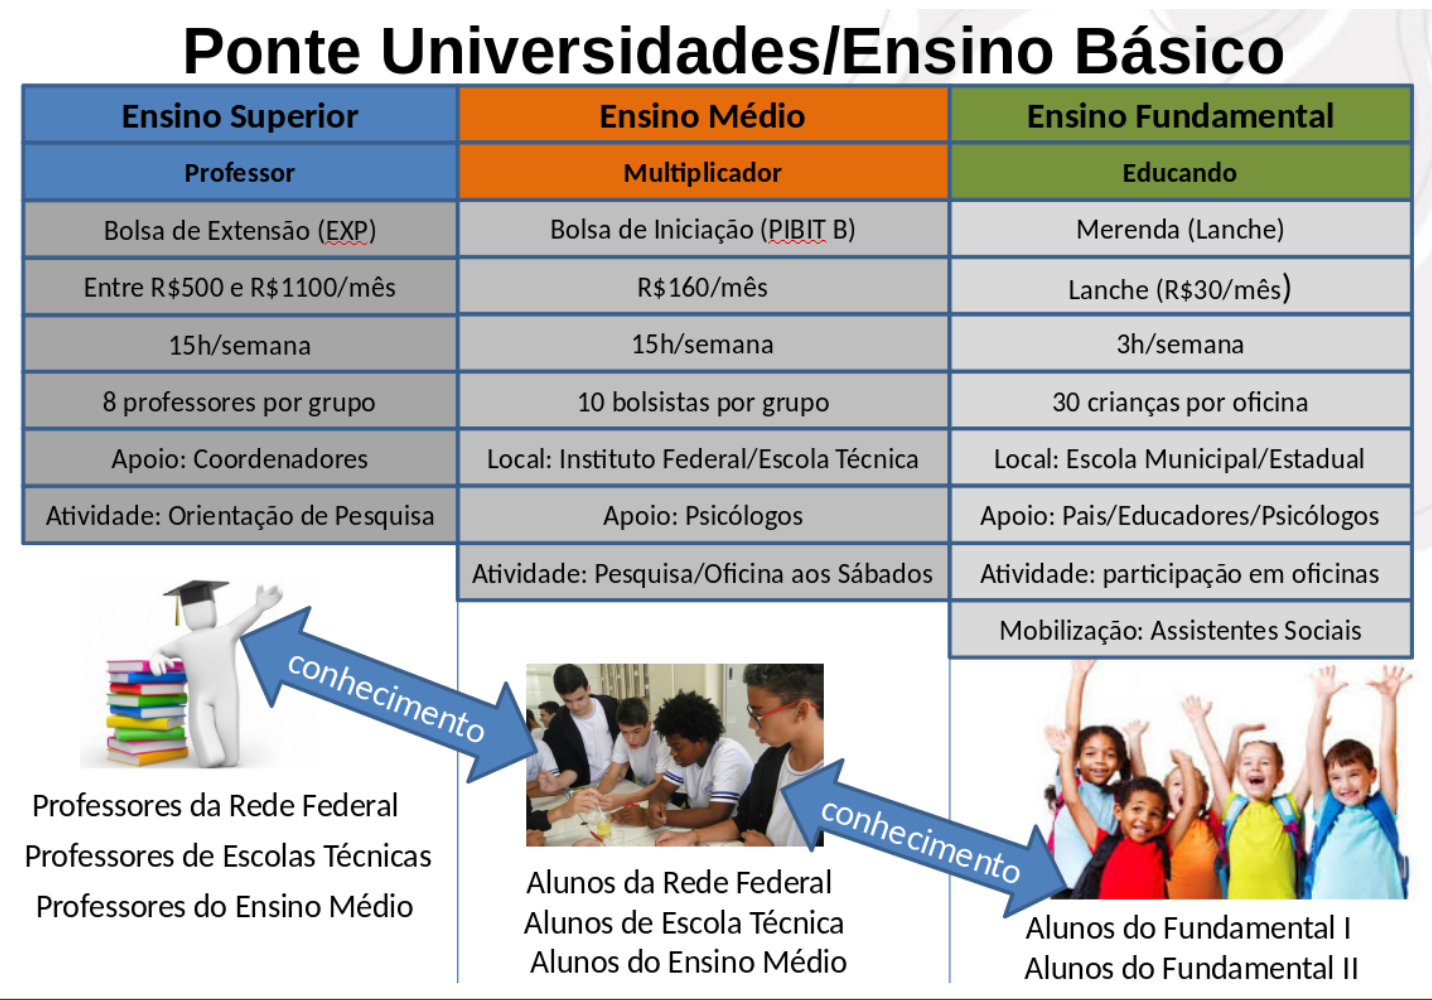
\includegraphics[max size={\textwidth}{\textheight}]{../../imagens/ponte-wash.png}

	\end{center}

	\caption{\label{061843808cd4a78f12d61af45200969bc8abf5ca}Diagrama mostrando o conceito de ponte entre centros de excel\^encia e o ensino fundamental, do WASH. (fonte: apresenta\c{c}\~ao de divulga\c{c}\~ao do WASH)}

\end{figure}

O diagrama da figura mostra que a dita \textquotedbl\{\}ponte\textquotedbl\{\}, uma met\'afora para indicar rela\c{c}\~oes entre institui\c{c}\~oes, est\'a estruturada em tr\^es n\'{\i}veis:













\begin{alineas}
\item n\'{\i}vel superior: educadores(as) do ensino superior, do ensino t\'ecnico e do ensino m\'edio s\~ao convidados a orientar projetos de inicia\c{c}\~ao cient\'{\i}fica de alunos(as) do ensino superior, t\'ecnico e m\'edio, com o compromisso de que uma parte do tempo do(a) aluno(a) seja dedicada para a realiza\c{c}\~ao de oficinas de dissemina\c{c}\~ao da ci\^encia no ensino fundamental;
\item n\'{\i}vel m\'edio, t\'ecnico e gradua\c{c}\~ao: s\~ao oferecidas bolsas de inicia\c{c}\~ao cient\'{\i}fica para alunos (as) do n\'{\i}vel m\'edio de escolas p\'ublicas, bem como alunos (as) do n\'{\i}vel superior e de escolas t\'ecnicas, cujos projetos ser\~ao orientados por educadores(as) do n\'{\i}vel superior. O(a) aluno(a) do ensino m\'edio, do ensino superior e das escolas t\'ecnicas que recebe bolsa se compromete a realizar oficinas no ensino fundamental, com o objetivo de disseminar conhecimentos aprendidos no WASH. As atividades com menores de idade s\~ao sempre supervisionadas por adultos(as) que tenham a  atribui\c{c}\~ao de responsabilidade pelos(as) menores de idade;e
\item n\'{\i}vel fundamental: por meio de um processo de mobiliza\c{c}\~ao, s\~ao identificadas as escolas, organiza\c{c}\~oes sociais que tenham interesse em disponibilizar as oficinas do WASH para suas crian\c{c}as. O Documento de Refer\^encia anexo \`a Portaria CTI 178/2018 \'e o instrumento que d\'a os par\^ametros de conduta para essa atividade, buscando torn\'a-la proveitosa e segura para todos os part\'{\i}cipes.

\end{alineas}

Com esse trabalho, podemos dizer, de forma simplificada, que o WASH \'e um Programa de Inicia\c{c}\~ao Cient\'{\i}fica com uma caracter\'{\i}stica especial: o aluno de inicia\c{c}\~ao assume o compromisso de multiplicar seus conhecimentos, participando como monitor de oficinas nas escolas de ensino fundamental ou outros tipos de institui\c{c}\~oes voltadas para educa\c{c}\~ao de menores de idade.












Este entendimento se coaduna com as inten\c{c}\~oes declaradas na Portaria CTI 178/2018, que \'e o Documento de Refer\^encia do Programa:













\noindent\begin{center}\mbox{\centering\fbox{\centering\par\parbox{0.7\linewidth}{\small\textit{\textquotedbl\{\}S\~ao os bolsistas de inicia\c{c}\~ao cient\'{\i}fica, que executam projetos de pesquisa, coordenados pelos orientadores (as). Os projetos s\~ao desenvolvidos, durante a semana, no ambiente de  estudo e pesquisa (normalmente na Entidade Promotora). Os bolsistas atuam, tamb\'em, como monitores dos educandos, sempre no contraturno da escola regular, atrav\'es da realiza\c{c}\~ao de oficinas. As duas atividades (inicia\c{c}\~ao cient\'{\i}fica e monitoria) devem ocupar no m\'aximo 15 horas semanais dos bolsistas.\textquotedbl\{\} (fonte: Portaria CTI 178/2018);}\normalsize}}}\end{center}


O Programa WASH, como visionado na avalia\c{c}\~ao do PID, \'e substancialmente financiado por meio de emendas parlamentares do Legislativo Federal, seguindo a bem-sucedida experi\^encia da Secretaria de Ci\^encia e Tecnologia para a Inclus\~ao Social- SECIS/MCT de financiar a inclus\~ao social, entre 2005 e 2009, por recursos com origem externa ao MCT da \'epoca. Essa caracter\'{\i}stica est\'a explicitada na Portaria CTI 178/2018:













\noindent\begin{center}\mbox{\centering\fbox{\centering\par\parbox{0.7\linewidth}{\small\textit{\textquotedbl\{\}O presente Programa (WASH) \'e substancialmente mantido por recursos oriundos de emendas parlamentares, que disponibilizam recursos financeiros  para o pagamento da maior parte das bolsas. Anualmente, os deputados podem indicar as emendas para o Programa WASH. Para conquistar este apoio, o interessado deve enviar ao gabinete do Deputado um of\'{\i}cio apresentando o Programa, de forma a formalizar a solicita\c{c}\~ao de emenda.\textquotedbl\{\} (fonte: Portaria CTI 178/2018)1}\normalsize}}}\end{center}


Identificamos 16 emendas aportadas ao WASH, as quais est\~ao listadas na se\c{c}\~ao deste cap\'{\i}tulo dedicada ao eixo 2.












As emendas, obtidas junto aos deputados federais, s\~ao direcionadas ao CNPq, que \'e o \'org\~ao respons\'avel pelo financiamento dos projetos de pesquisa e extens\~ao; e para cada emenda recebida \'e elaborado um projeto espec\'{\i}fico, como tamb\'em indicado na Portaria CTI 178/2018:













\noindent\begin{center}\mbox{\centering\fbox{\centering\par\parbox{0.7\linewidth}{\small\textit{\textquotedbl\{\}\'Org\~ao Executor: Conselho Nacional de Desenvolvimento Cient\'{\i}fico e Tecnol\'ogico (CNPq), entidade ao qual s\~ao destinados os recursos provenientes de emendas parlamentares para custeio do Programa WASH.\textquotedbl\{\} (fonte: Portaria CTI 178/2018)}\normalsize}}}\end{center}


Como estipulado pela Portaria CTI 178/2018, o Programa WASH estabelece pap\'eis a serem desempenhados pelos participantes, como segue:













\begin{alineas}
\item Coordenador: \textquotedbl\{\}Servidor, professor, cientista ou pesquisador respons\'avel pelo Programa WASH e interlocu\c{c}\~ao junto ao CNPq, incluindo a elabora\c{c}\~ao do Plano de Trabalho do Projeto\textquotedbl\{\}  (CTI, 2018) . Este papel vem sendo desempenhado pelo Dr. Victor Pellegrini Mammana. Observa-se uma crescente delega\c{c}\~ao dessas tarefas para os part\'{\i}cipes mais experientes do Programa. Dentre as atividades que devem ser desempenhadas pelo coordenador est\~ao: \textquotedbl\{\}inscrever e fazer gest\~ao da Plataforma Carlos Chagas com as indica\c{c}\~oes das bolsas. \'E o respons\'avel por solicitar prorroga\c{c}\~ao da execu\c{c}\~ao da emenda se houver necessidade, buscar financiamento para o Programa.\textquotedbl\{\}  (CTI, 2018) Al\'em dessas responsabilidades expressas no termo de refer\^encia, observamos ao longo de nossa experi\^encia outras, tais como: elaborar os relat\'orios para o CNPq, bem como a presta\c{c}\~ao de contas, com um minucioso trabalho de avalia\c{c}\~ao do desempenho de todos os bolsistas do projeto. Tamb\'em, soma-se \`as demais atividades o papel de encontrar novas institui\c{c}\~oes interessadas em realizar o Programa, buscando novas parcerias, assim como novos parlamentares interessados em financi\'a-lo. Observa-se que estas atividades t\^em recebido apoio dos demais colaboradores do WASH.
\item Coordenador local: \textquotedbl\{\}Respons\'avel por implementar o Programa junto aos interessados. Incluem-se dentre as suas atribui\c{c}\~oes: organizar e planejar as oficinas; preparar as reuni\~oes das equipes locais; planejar e promover as oficinas de multiplica\c{c}\~ao com as crian\c{c}as; elaborar com os orientadores e bolsistas os conte\'udos/temas das oficinas; monitorar a elabora\c{c}\~ao conjunta pelos orientadores e bolsistas dos planos de trabalho espec\'{\i}ficos pelos orientadores e bolsistas, apresentando-os para o coordenador do programa junto ao CNPq; elaborar os relat\'orios de gest\~ao do Programa; registrar a presen\c{c}a dos participantes;; organizar a participa\c{c}\~ao dos educandos e bolsistas na Semana Nacional de Ci\^encia e Tecnologia-SNCT e outros eventos similares.\textquotedbl\{\}  (CTI, 2018)
\item Monitor(a) ou Bolsista: \textquotedbl\{\} S\~ao os bolsistas de inicia\c{c}\~ao cient\'{\i}fica que executam projetos, de pesquisa coordenados pelos orientadores. Os projetos s\~ao desenvolvidos durante a semana, no ambiente de pesquisa (normalmente, na Entidade Promotora). Os bolsistas atuam, tamb\'em, como monitores dos educandos, sempre no contraturno da escola regular, atrav\'es da realiza\c{c}\~ao de oficinas. As duas atividades (Inicia\c{c}\~ao Cient\'{\i}fica e monitoria) devem ocupar no m\'aximo 15 horas semanais dos bolsistas. Respons\'avel por registrar os conte\'udos das oficinas no site do MIT (Scratch) e demais instrumentos de registro.\textquotedbl\{\}  (CTI, 2018)
\item Orientador (a): \textquotedbl\{\}Respons\'avel pela orienta\c{c}\~ao cient\'{\i}fica e metodol\'ogica, tanto na elabora\c{c}\~ao quanto na execu\c{c}\~ao dos planos de trabalho dos bolsistas/monitores, no Programa. Respons\'avel pela participa\c{c}\~ao em eventos de ci\^encia e tecnologia (congressos, Semana Nacional de Ci\^encia e Tecnologia) etc.
\item Educando: \textquotedbl\{\}Protagonista do fen\^omeno de aprendizagem. No presente contexto, o educando \'e o estudante do ensino fundamental que participa das oficinas.\textquotedbl\{\}  (CTI, 2018) Nossa experi\^encia mostra que este papel \'e desempenhado, principalmente, por alunos do ensino fundamental.
\end{alineas}

Durante a experi\^encia desta autora com a forma de executar o WASH no per\'{\i}odo anterior \`a pandemia de 2020, foi poss\'{\i}vel constatar que as oficinas se davam exclusivamente na forma presencial. Do ponto de vista formal, a Portaria CTI 178/2018 indica  a forma de realiza\c{c}\~ao das oficinas:













\noindent\begin{center}\mbox{\centering\fbox{\centering\par\parbox{0.7\linewidth}{\small\textit{\textquotedbl\{\}Oficina: Atividade de intera\c{c}\~ao humana que envolve quantidade de pessoas pr\'e-determinada, com dura\c{c}\~ao fixa e data definida, executada por equipe composta por coordenador local, orientadores e monitores/bolsistas (ver adiante), com \^enfase em conte\'udo ou n\~ao, durante a qual busca-se o protagonismo do educando no processo de aprendizagem.\textquotedbl\{\} (fonte: Portaria CTI 178/2018)}\normalsize}}}\end{center}


A \^enfase dada pela Portaria CTI 178/2018 \`a \textquotedbl\{\}presen\c{c}a\textquotedbl\{\} dos part\'{\i}cipes nas \textquotedbl\{\}viv\^encias\textquotedbl\{\}, ou oficinas, nos permite depreender que o WASH foi concebido para ser exclusivamente presencial. Esta concep\c{c}\~ao gerou dificuldades para o Programa no auge do isolamento social, durante a pandemia, e esse \'e um dos pontos que precisa ser tratado na revis\~ao do Documento de Refer\^encia do WASH.












No que tange \`a classifica\c{c}\~ao das institui\c{c}\~oes part\'{\i}cipes, a Portaria CTI 178/2018 explicita os seguintes tipos:













\begin{alineas}
\item \'Org\~ao Executor: usando uma terminologia caracter\'{\i}stica da gest\~ao p\'ublica, o CNPq \'e o \'org\~ao executor do WASH, uma vez que executa o or\c{c}amento viabilizado pelas emendas parlamentares.
\item \'Org\~ao Coexecutor: tamb\'em, no contexto da linguagem caracter\'{\i}stica do setor p\'ublico pode existir um \'org\~ao coexecutor dos recursos, papel que, na situa\c{c}\~ao em que o projeto estava em 2018, era desempenhado pelo CTI Renato Archer. Essa situa\c{c}\~ao n\~ao est\'a mais presente, uma vez que o coordenador dos projetos CNPq associados ao WASH n\~ao est\'a mais vinculado a aquela institui\c{c}\~ao, havendo que se rever esse aspecto no Documento de refer\^encia do Programa.
\item Entidade Promotora: \textquotedbl\{\}Institui\c{c}\~ao p\'ublica de educa\c{c}\~ao ou pesquisa (federal, estadual ou municipal) cuja miss\~ao estatut\'aria envolva a educa\c{c}\~ao e/ou a dissemina\c{c}\~ao da ci\^encia, incluindo Institui\c{c}\~oes Cient\'{\i}ficas, Tecnol\'ogicas e de Inova\c{c}\~ao (ICTs).\textquotedbl\{\} (CTI, 2018). Na concep\c{c}\~ao do WASH, a experi\^encia do CTI norteou muito a \textquotedbl\{\} liturgia \textquotedbl\{\} das atividades, havendo uma \^enfase na realiza\c{c}\~ao das atividades no contraturno, situa\c{c}\~ao em que era necess\'ario oferecer transporte e alimenta\c{c}\~ao para os participantes. Com a evolu\c{c}\~ao do Programa, sua atividades foram sendo integradas ao turno escolar, requerendo menor \^enfase no apoio ao transporte e alimenta\c{c}\~ao, j\'a oferecido pelas escolas part\'{\i}cipes (Entidades Respons\'aveis). Ao longo de uma d\'ecada, muitos tipos de institui\c{c}\~oes desempenharam o papel de Entidades Promotoras: Institutos Federais (e.g. IFSP Campinas, IFSP Campos do Jord\~ao, IFSP Jacare\'{\i}, IFSP S\~ao Jos\'e dos Campos, etc), Unidades de Pesquisa (CTI Renato Archer e CEMADEN), Universidades Estaduais (UNICAMP e USP), Universidades Federais (UFABC e UNIFESP), dentre tantas outras.
\item Entidade Respons\'avel: na Portaria CTI 178/2018, a institui\c{c}\~ao respons\'avel \'e \textquotedbl\{\}institui\c{c}\~ao p\'ublica (federal, estadual, municipal), ou entidades da sociedade civil sem fins lucrativos que tenham infraestrutura adequada para o oferecimento das oficinas.\textquotedbl\{\}  (CTI, 2018)  Com a evolu\c{c}\~ao do Programa, decidiu-se por aceitar como entidades respons\'aveis apenas aquelas que tivessem, al\'em da infraestrutura para as oficinas, a atribui\c{c}\~ao legal de responsabilidade pelos menos do ensino fundamental. Essa medida foi um aprimoramento da divis\~ao de responsabilidades, garantindo que apenas profissionais habilitados e legalmente autorizados assumissem a responsabilidade de \textquotedbl\{\}cuidar de crian\c{c}as\textquotedbl\{\}. No formato inicial, na aus\^encia de um profissional com essas caracter\'{\i}sticas, era exigida a presen\c{c}a de pelo menos um respons\'avel dos educandos, com a autoriza\c{c}\~ao dos demais, durante as oficinas. S\~ao exemplos de entidades respons\'aveis: as escolas municipais e estaduais, os sindicatos com escolas autorizadas (e.g. Dona Lind\'u), as igrejas, entre outras.
\end{alineas}

O WASH optou por n\~ao utilizar o instrumento de conv\^enio para disseminar suas pr\'aticas nas entidades promotoras e respons\'aveis. O motivo \'e a lentid\~ao do instrumento, Nossa experi\^encia de gest\~ao junto ao CTI Renato Archer, entre 2013 e 2018, quando esta autora foi secret\'aria executiva da  diretoria, mostrou que o estabelecimento de um conv\^enio entre entes federados pode levar meses; frequentemente, mais do que seis meses para ser assinado. Isso porque h\'a v\'arias inst\^ancias pelas quais o processo administrativo deve passar, entre elas a AGU.












Um conv\^enio \'e um tipo de \textquotedbl\{\}contrato\textquotedbl\{\} em que part\'{\i}cipes (e n\~ao partes) buscam um objetivo comum, estabelecendo direitos e obriga\c{c}\~oes. Avaliamos no in\'{\i}cio do Programa que este tipo de instrumento poderia ser dispensado se houvesse o cuidado de escolher entidades respons\'aveis que j\'a tivessem em sua miss\~ao a educa\c{c}\~ao, ao passo que houvesse, tamb\'em, o cuidado de escolher entidades promotoras que j\'a tivessem em sua miss\~ao a extens\~ao. Para garantir a agilidade da dissemina\c{c}\~ao, o WASH concebeu a ideia de \textquotedbl\{\}Documento de Refer\^encia\textquotedbl\{\}, que deveria ser citado em um termo de ades\~ao publicado pela entidade interessada em participar (promotora ou respons\'avel). Por meio desta publica\c{c}\~ao seriam assumidos compromissos com a metodologia do WASH, sem a necessidade do Conv\^enio, cabendo \`a entidade signat\'aria arcar com os \^onus dessa declara\c{c}\~ao p\'ublica. Essa ideia se mostrou bastante exitosa, como pode ser verificada pela lista de \textquotedbl\{\}termos de ades\~ao\textquotedbl\{\} publicadas pelos part\'{\i}cipes do WASH (ver neste Cap\'{\i}tulo a parte referente ao eixo 2).












\subsection[WASH na pandemia]{WASH na pandemia}\label{WASH na pandemia}
Vimos que o a Portaria CTI 178/2018 enfatiza a quest\~ao da \textquotedbl\{\}presen\c{c}a\textquotedbl\{\}, ao descrever as viv\^encias do WASH e, como testemunhado por esta autora, fato verific\'avel pela Plataforma Platu\'oxe, o Programa n\~ao realizava atividades \`a dist\^ancia antes da pandemia da covid.












Sabe-se que esse era um des\'{\i}gnio do coordenador do WASH, cujas declara\c{c}\~oes sobre a import\^ancia de manter o WASH como atividade presencial foram testemunhadas por todos os que participavam de reuni\~oes de Coordena\c{c}\~ao ao longo dos v\'arios anos do Programa. Justificava essa inten\c{c}\~ao pelo que tinha vivenciado nas visitas que fizera \`as oficinas promovidas por colaboradores de David Cavallo, em Massachussets, durante a avalia\c{c}\~ao do OLPC. David Cavallo era ativista do pensamento de Papert, contato de Afira Ripper no MIT e membro do OLPC, de Negroponte.












Na avalia\c{c}\~ao do PID  (CGEE, 2010a), ficava clara a predile\c{c}\~ao do coordenador do WASH pelo conceito de educa\c{c}\~ao como resultado da intera\c{c}\~ao entre indiv\'{\i}duos. Na avalia\c{c}\~ao OLPC, ele indicava a dificuldade de representar digitalmente todos os aspectos da intera\c{c}\~ao humana.












No entanto, a realidade da pandemia se imp\^os, impedindo a realiza\c{c}\~ao de atividades presenciais do Programa durante por mais de um ano. J\'a no primeiro semestre de 2020, assim que a gravidade da pandemia ficou evidente, foram tomadas medidas emergenciais para garantir a execu\c{c}\~ao das emendas parlamentares, mesmo no contexto de isolamento social.












Duas iniciativas se estabeleceram imediatamente:













\begin{alineas}
\item Oficinas remotas ass\'{\i}ncronas: o coordenador do Programa WASH iniciou experimentos utilizando o WhatsApp. Para isso contou com a iniciativa da Profa. Daniele de Souza Silva de experimentar uma nova forma de trabalho. A Profa. Daniele era da rede municipal de Educa\c{c}\~ao da cidade de Jacare\'{\i}, onde se desenvolveram os primeiros pilotos. A escola tinha poucos recursos, sem possibilidade de fornecer qualquer tipo de equipamento de inform\'atica aos estudantes, requerendo um modelo de oficina que pudesse ser realizado de forma ass\'{\i}ncrona, utilizando o celular dos respons\'aveis (pais, m\~aes, etc). A ideia era inverter a atividade de programa\c{c}\~ao de jogos, atribuindo aos alunos a especifica\c{c}\~ao do jogo, com a cria\c{c}\~ao das personagens. A programa\c{c}\~ao dos jogos, seguindo a especifica\c{c}\~ao das crian\c{c}as, seria feita em seguida, pelos bolsistas do WASH; tamb\'em remotamente, uma vez que estes tinham mais acesso a computadores. A experi\^encia, inicialmente limitada, resultou na produ\c{c}\~ao de um jogo e audiovisuais, descrevendo o que estava sendo feito, com a participa\c{c}\~ao dos educandos. Essa iniciativa foi depois aprimorada pelos bolsistas Michel Alencar Morandi e Ana Carolina de Deus Soares, tendo sido reproduzida em outras escolas.
\item \textquotedbl\{\}Ci\^encia e Cultura, vamos brincar?\textquotedbl\{\}  (TOZZI, 2021): \'e uma webs\'erie idealizada  e coordenada por essa  autora e produzida com o Movimento N\'os Somos a Ci\^encia e a Companhia Cultural Bola de Meia. A webs\'erie resguarda o m\'etodo cient\'{\i}fico e a cada epis\'odio  busca  alinhar as tem\'aticas cientificas \`as manifesta\c{c}\~oes  da cultura popular.  Foram criados e produzidos audiovisuais em n\'{\i}vel profissional, com diversas express\~oes e linguagens culturais  com a perspectiva de preservar a cultura da inf\^ancia; e ao mesmo tempo,  cultivar pr\'aticas cient\'{\i}ficas.  Os educandos com seus familiares tiveram a oportunidade de usufruir de uma programa\c{c}\~ao cientifica cultural para um p\'ublico 
intergeracional. Neste trabalho, foi poss\'{\i}vel dar visibilidade \`as pr\'aticas STEAM do WASH,  \`as entrevistas com cientistas renomados, conte\'udos tais como ci\^encia, m\'usica, conta\c{c}\~ao de hist\'orias, quadros do tipo \textquotedbl\{\}fa\c{c}a voc\^e mesmo\textquotedbl\{\} e entrevistas. Essa programa\c{c}\~ao foi denominada \textquotedbl\{\}Ci\^encia e Cultura, Vamos Brincar?\textquotedbl\{\} (CCVB) e foi disponibilizada em v\'arios meios (Youtube e TV Aberta). A Fig. 29 mostra o pedido de autoriza\c{c}\~ao para veicula\c{c}\~ao da webs\'erie pela TVT. Outros pedidos semelhantes foram formulados. Foram nove epis\'odios, os quais est\~ao listados na parte destinada ao eixo 2 deste cap\'{\i}tulo. Esta produ\c{c}\~ao contou com a participa\c{c}\~ao de uma ampla equipe, coordenada pela a autora. Os trabalhos foram concomitantes com o per\'{\i}odo em que esta autora esteve matriculada no mestrado, podendo ser considerados como um dos produtos educacionais da presente disserta\c{c}\~ao, raz\~ao pela qual \'e detalhada no cap\'{\i}tulo de Produtos Educacionais.
\end{alineas}



\captionsetup{format=plain}
\begin{figure}[max size={\textwidth}{\textheight}]

\centering


\begin{minipage}[b]{0.4\linewidth}
        \centering
                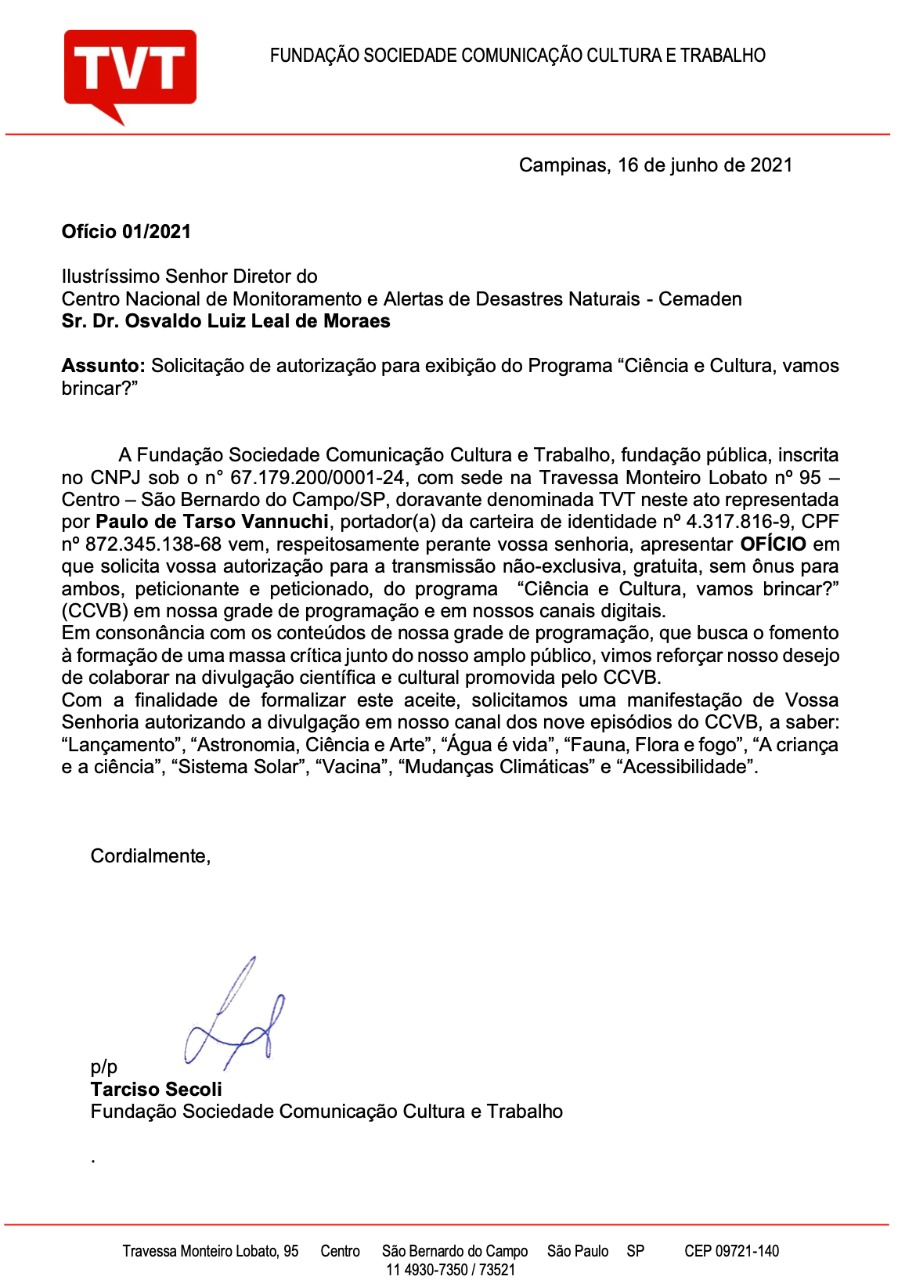
\includegraphics[width=1.0\linewidth]{../../imagens/TVT.jpg}
                \caption{Documento de solicita\c{c}\~ao de autoriza\c{c}\~ao para a veicula\c{c}\~ao da webs\'erie Ci\^encia e Cultura, vamos brincar?, exemplificando o interesse de TVs-web e abertas pela programa\c{c}\~ao criada pelo WASH. (fonte: acervo do WASH)}
                \label{51f9418c1ca6e2404e9d774513fb6c023d10b3bb}
\end{minipage}%
\hspace{0.5cm}
\end{figure}



A introdu\c{c}\~ao de atividades remotas no WASH, como resultado da experi\^encia da pandemia, \'e uma das justificativas para a revis\~ao do documento de refer\^encia.












\section[Caracteriza\c{c}\~ao dos Indicadores do WASH (eixo 2)]{Caracteriza\c{c}\~ao dos Indicadores do WASH (eixo 2)}\label{Caracteriza\c{c}\~ao dos Indicadores do WASH (eixo 2)}
Na se\c{c}\~ao da Fundamenta\c{c}\~ao Te\'orica, embasamos os conceitos de \textquotedbl\{\}dados\textquotedbl\{\}, \textquotedbl\{\}informa\c{c}\~oes\textquotedbl\{\} e \textquotedbl\{\}conhecimento\textquotedbl\{\}  atrav\'es da refer\^encia  Setzer e Silva (2017). Tra\c{c}ando um paralelo com aqueles conceitos, podemos dizer que o objetivo da realiza\c{c}\~ao de consultas estruturadas, via Plataforma \textquotedbl\{\}Platu\'oxe\textquotedbl\{\}, \'e produzir informa\c{c}\~oes, na forma de indicadores, os quais, analisados e interpretados, levar\~ao \`a produ\c{c}\~ao dos conhecimentos sobre objeto de estudo. Estes conhecimentos permitir\~ao avaliar as Hip\'oteses 1, 2, 4, 5 e 6.












Considerando os conceitos definidos na se\c{c}\~ao 2.3, da Fundamenta\c{c}\~ao Te\'orica (eventos, emendas parlamentares, planos de trabalho, relat\'orios e inicia\c{c}\~ao cient\'{\i}fica), s\~ao exemplos de indicadores a serem apresentados nesta se\c{c}\~ao:













\begin{alineas}
\item quantidade de emendas parlamentares concedidas ao WASH;
\item quantidade de termos de ades\~ao ao WASH;
\item estimativa do n\'umero de pessoas atendidas;
\item evolu\c{c}\~ao temporal do n\'umero de pessoas atendidas (participa\c{c}\~oes);
\item participantes por sexo (indicador de equidade);
\item n\'umero de bolsistas;
\item temas nos planos de trabalho e relat\'orios das inicia\c{c}\~oes cient\'{\i}ficas;
\item quantidade de eventos realizadas;
\item perfil et\'ario dos participantes em eventos;
\item distribui\c{c}\~ao de temas nos eventos;
\item distribui\c{c}\~ao das atividades nos eventos;
\item quantidade de cidades atendidas; e
\item produ\c{c}\~ao audiovisual.
\end{alineas}

Importante registrar que os indicadores foram obtidos a partir da contribui\c{c}\~ao de v\'arios colaboradores do WASH, que elaboraram os c\'odigos em SQL, para as consultas estruturadas, a partir de nossa especifica\c{c}\~ao.












Entretanto, o trabalho de produ\c{c}\~ao de indicadores n\~ao se restringiu \`a \textquotedbl\{\} Platu\'oxe\textquotedbl\{\} e outras tr\^es fontes de dados foram utilizadas:













\begin{alineas}
\item Plataforma de Planejamento Financeiro do Programa WASH: instrumento para acompanhamento das concess\~oes de bolsas, seus prazos e validades, documentos de outorgas e planos de trabalho. Trata-se de uma ferramenta de compliance e presta\c{c}\~ao de contas de cada projeto, mas que, tamb\'em, pode ser usada para a caracteriza\c{c}\~ao dos mesmos, pela abrang\^encia dos dados nela contida;
\item Planilhas eletr\^onicas: constru\'{\i}das  manualmente para viabilizar a verifica\c{c}\~ao dos dados das demais plataformas, uma vez que foram identificadas algumas fragilidades nas demais fontes de informa\c{c}\~oes;e

\item Acervo de documentos usados tamb\'em no \^ambito do eixo 1 (hist\'oria), bem como plataformas de entidades p\'ublicas, a exemplo da Plataforma Carlos Chagas do CNPq  (CHAGAS, 2022).
\end{alineas}

Dois recortes temporais foram adotados, como j\'a explicitado em Materiais e M\'etodos:













\begin{alineas}
\item Recorte A da Platu\'oxe, de setembro de 2013 a agosto de 2022 (congelada); e
\item Recorte B da Platu\'oxe, de setembro de 2013 a janeiro de 2023 (alimentada em tempo real).
\end{alineas}

\subsection[Lista de Emendas Parlamentares concedidas]{Lista de Emendas Parlamentares concedidas}\label{Lista de Emendas Parlamentares concedidas}
No eixo 1, identificamos que o WASH tem como fonte de financiamento principal as emendas parlamentares do Legislativo Federal, mas a lista completa ainda n\~ao foi apresentada.












Para levantar as listas, usamos como fonte a Plataforma Carlos Chagas do CNPq (CHAGAS, 2022), sendo poss\'{\i}vel constatar a exist\^encia das seguintes emendas concedidas ao WASH:













\begin{alineas}
\item \textquotedbl\{\}Programa WASH, emenda concedida pelo Deputado Federal Ivan Valente, em 2016;
\item \textquotedbl\{\}Programa WASH!\textquotedbl\{\}, emenda concedida pelo Deputado Ivan Valente, em 2017;
\item \textquotedbl\{\}Forma\c{c}\~ao em Captura de Movimentos\textquotedbl\{\}, emenda concedida pelo Deputado Federal Alex Canziani, em 2018;
\item \textquotedbl\{\}Cinema de anima\c{c}\~ao 3D e desenvolvimento de jogos com a ferramenta Blender e o Programa WASH\textquotedbl\{\}, emenda concedida pelo Deputado Alex Canziani, em 2019;
\item \textquotedbl\{\}Programa WASH no Paran\'a\textquotedbl\{\}, emenda concedida, em 2020, pelo Deputado Alex Canziani;
\item \textquotedbl\{\}PROGRAMA WASH-STEAM NO ESTADO DE S\~AO PAULO: Promo\c{c}\~ao da Ci\^encia, 
Tecnologia, Engenharia, Artes  e Matem\'atica na Rede P\'ublica de Ensino\textquotedbl\{\}, emenda concedida pelo Deputado Federal, Ivan Valente, em 2020;

\item \textquotedbl\{\}Regi\~oes Metropolitanas\textquotedbl\{\}, emenda parlamentar concedida, pelo Deputado Federal Alexandre Padilha, em 2020;
\item \textquotedbl\{\}Redes de Aprendizagem\textquotedbl\{\}, emenda concedida, em 2020, pelo Deputado Federal Ivan Valente;
\item \textquotedbl\{\}Programa WASH - Lei Aldir Blanc\textquotedbl\{\}, emenda parlamentar concedida, pelo Deputado Federal  Ivan Valente, em 2020;
\item \textquotedbl\{\}Programa WASH em Campos do Jord\~ao\textquotedbl\{\}, emenda parlamentar concedida, pelo Deputado Federal Eduardo Cury, em 2020;
\item \textquotedbl\{\}Programa WASH no ABC\textquotedbl\{\}, emenda parlamentar concedida, pelo Deputado Federal Vicentinho em 2022;
\item \textquotedbl\{\}WASH na USP\textquotedbl\{\}, emenda parlamentar concedida; pelo Deputado Federal Orlando Silva, em 2022;
\item \textquotedbl\{\}WASH na UFABC\textquotedbl\{\}, emenda parlamentar concedida, pelo Deputado Federal Alexandre Padilha, em 2022;
\item \textquotedbl\{\}WASH em S\~ao Bernardo do Campo\textquotedbl\{\}, emenda concedida, pelo Deputado Federal Carlos Zaratini, 2022 e
\item \textquotedbl\{\}Projeto Renato Archer\textquotedbl\{\}, emenda concedida, pelo Deputado Federal Ivan Valente, em 2022.
\end{alineas}

\subsection[Lista de Termos de Ades\~ao ao Programa WASH]{Lista de Termos de Ades\~ao ao Programa WASH}\label{Lista de Termos de Ades\~ao ao Programa WASH}
O WASH decidiu-se por n\~ao estabelecer o instrumento de Conv\^enio como meio de dissemina\c{c}\~ao do Programa. Essa decis\~ao foi decorrente do prazo excessivo para tramita\c{c}\~ao desse tipo de instrumento jur\'{\i}dico, que pode demorar v\'arios meses. Alternativamente, concebeu-se um formato de mobiliza\c{c}\~ao de outras institui\c{c}\~oes, baseado na ades\~ao por declara\c{c}\~oes  unilaterais, denominadas \textquotedbl\{\}ades\~oes\textquotedbl\{\}.












Combinando a busca na \textquotedbl\{\}Platu\'oxe\textquotedbl\{\} com a busca no cervo, identificamos os seguintes tipos de documentos de ades\~ao:  edi\c{c}\~ao de portarias, termos de ades\~ao, boletins, atas deliberativas de reuni\~oes de conselhos de escolas e de sa\'ude, manifesta\c{c}\~oes por of\'{\i}cios, enfim: documentos editados pelas entidades interessadas no Programa, que se configuram como atos de gest\~ao.












Abaixo, apresentamos, organizadas por tipos de institui\c{c}\~oes, as ades\~oes encontradas pela autora, nos registros do WASH.












No que se refere a \textquotedbl\{\}unidades de pesquisa\textquotedbl\{\}, identificamos os seguintes documentos:













\begin{alineas}
\item Centro de Tecnologia da Informa\c{c}\~ao Renato Archer - CTI - proponente inicial da metodologia, por meio da Portaria CTI 178/2018, como j\'a amplamente mencionado ao longo do texto:
\item CEMADEN - Portaria No. 144/2019/SEI-CEMADEN, de 02/12/2019 - Institui o Programa CEMADEN Educa\c{c}\~ao, define sua estrutura e formas de implementa\c{c}\~ao, e d\'a outras provid\^encias. A Portaria traz em seu Art 3o.: O Programa Cemaden Educa\c{c}\~ao adotar\'a como uma de suas formas de execu\c{c}\~ao o termo de refer\^encia do Programa WASH - Workshop Aficionados em Software e Hardware, conforme consta do Anexo I da Portaria, n° 178/2018/SEI-CTI, de 12 de novembro de 2018, promovendo a integra\c{c}\~ao das tem\'aticas de ci\^encia, tecnologia, matem\'atica, arte e engenharia, inerentes a aquele Programa, com as demais caracter\'{\i}sticas e tem\'aticas do Cemaden Educa\c{c}\~ao, realizando adapta\c{c}\~oes did\'aticas quando couber, conforme previsto no Anexo, I desta Portaria.
\end{alineas}

Na esfera municipal, identificamos  v\'arias formas de ades\~ao do Poder Executivo. Os casos mais emblem\'aticos s\~ao aqueles que se deram pela aprova\c{c}\~ao de leis municipais, como ocorreu nas cidades de Prado Ferreira e Dr. Camargo, no Estado do Paran\'a. Nestas duas iniciativas independentes, identificamos o protagonismo de duas autoridades p\'ublicas com grande comprometimento com a educa\c{c}\~ao em suas cidades, o ent\~ao prefeito, Silvio Damasceno, de Prado Ferreira; e a vereadora, Valdirene Maria dos Santos (Dila)  de Dr. Camargo. Nas demais cidades, observamos a utiliza\c{c}\~ao dos instrumentos de portaria, normalmente editada pelas secretarias de educa\c{c}\~ao. A participa\c{c}\~ao de Campinas, que envolveu o Observat\'orio Municipal, foi o \'unico caso de utiliza\c{c}\~ao de conv\^enio, como se v\^e na lista, a seguir:













\begin{alineas}
\item JACARE\'I - Secretaria Municipal de Educa\c{c}\~ao - Portaria 3865, de 20/02/2020. Adota a Metodologia do Programa WASH nas atividades pedag\'ogicas da Secretaria Municipal de Educa\c{c}\~ao de Jacare\'{\i} (Publicada no Boletim Oficial do Munic\'{\i}pio de Jacare\'{\i}, em 21/02/2020);
\item MUNIC\'IPIO DE DR. CAMARGO - Lei no.1601 de 2021-Institui a metodologia WASH como pol\'{\i}tica p\'ublica no munic\'{\i}pio paranaense, Dr. Camargo. Link: http://www.doutorcamargo.pr.gov.br/
\item MUNIC\'IPIO DE PRADO DE FERREIRA - LEI No. 496, DE 16 DE ABRIL DE 2019 - Institui o Programa Profiss\~ao 4.0 para a capacita\c{c}\~ao e orienta\c{c}\~ao profissional destinadas \`as crian\c{c}as, jovens e adultos do munic\'{\i}pio de Prado Ferreira/PR.
\item SECRETARIA MUNICIPAL DE CULTURA DE CAMPINAS- Conv\^enio com o Observat\'orio Municipal Jean Nicolini, 2018:
\item SECRETARIA MUNICIPAL DE SANTO IN\'ACIO/ PR - Oficializa a ades\~ao ao Programa WASH em, 20/12/2021;
\end{alineas}

Foram identificadas ades\~oes das seguintes universidades federais/estaduais e Institutos Federais:













\begin{alineas}
\item UNIVERSIDADE DE S\~AO PAULO - USP - Portaria GR 7669, de 8/07/2021- Estabelece as condi\c{c}\~oes para a execu\c{c}\~ao do Programa WASH na Universidade de S\~ao Paulo;
\item UNIVERSIDADE TECNOL\'OGICA FEDERAL DO PARAN\'A - Portaria DO DIRETOR-GERAL - No. 147, 05/11/2020 - Adota a Portaria 178/2018/SEI/CTI, de 12/11/2018 como modelo de refer\^encia do Programa WASH, criando condi\c{c}\~oes para que a UTFPR, atue como entidade promotora;
\item FUNDA\c{C}\~AO UNIVERSIDADE FEDERAL DO ABC - Portaria 915/2020, DE 27/08/2020- Adota o Programa WASH na UFABC, publicada no Boletim de Servi\c{c}o no. 977, em 28/08/2020;
\item IF CAMPUS JACARE\'I (SP) - Portaria JCR.0031/2019 - abril de 2019 - Institui o Programa WASH no Campus Jacare\'{\i};
\item IF CAMPUS LONDRINA (PR) - Portaria 101, de 22/04/2019 - Adota a Portaria 178/2018/SEI/CTI, de 12/11/2018, como modelo de refer\^encia do Programa WASH, para que o IF-PR atue como entidade promotora;
\item IF CAMPUS CAMPINAS (SP) - Portaria CMP 0043/2019, de 24/04/2019 - Institui o Programa WASH no Campus Campinas;
\item IF CAMPUS SOROCABA  (SP) - Portaria SOR .0027/2019 - 25 abril de 2019 - Institui o Programa WASH no IFSP, Campus Sorocaba;
\item IF CAMPUS ARARAQUARA (SP) - Portaria no ARQ. 0042/2019, de 25 de abril de 2019 - Institui o Programa WASH no Campus Araraquara do IFSP;
\item IF CAMPUS SALTO (SP) Portaria SLT - 0061/2019 - de 06 de maio de 2019 - Institui o Programa WASH no Campus SALTO;
\item IF CAMPUS CUBAT\~AO (SP) Portaria CBT 055/2019 - de 27 de maio de 2019 - Institui o Programa WASH no Campus Cubat\~ao;
\item IF CAMPUS S\~AO JOS\'E DOS CAMPOS (SP) Portaria  SJC. 0083/2019, de 10/06/2019 - Designa membros para o Grupo de Trabalho para Programa WASH;
\item IF CAMPUS DE CAMPOS DO JORD\~AO (SP) Portaria CJO 0109/2019, de 16/10/2019- Designar membros para o programa WASH; e
\item IF CAMPUS CARAGUATATUBA (SP) Portaria 95/2021 DRG/CAR/IFSP, 25 de Novembro de 2021 - Designar o servidor Nelson Alvez Pinto para coordenar o Grupo de Trabalho (GT) para ado\c{c}\~ao da Metodologia WASH, no Campus de Caraguatatuba.
\end{alineas}

Foram identificadas as ades\~oes formais das seguintes escolas estaduais:













\begin{alineas}
\item E.E. Ernesto Monte - Bauru/SP
\item E.E. Expedito Camargo Freire - Campos do Jord\~ao/SP
\item E.E. Prof. Sebasti\~ao Inoc Assump\c{c}\~ao - Arealva/SP
\item E.E. Profa. Fanny Monzoni Santos - Osasco/SP
\item E.E. Prof. Hadia Feres - Carapicu\'{\i}ba/SP
\item E.E. Dr. \'Alvaro de Souza Lima - S\~ao Paulo/SP
\item E.E. Dinah L\'ucia Balestreiro - Brotas/SP  
\item E.E. Prof. Walmar Louren\c{c}o Santiago - S\~ao Jos\'e dos Campos/SP
\item E.E. Rubens Moreira da Rocha- Santo Andr\'e/SP
\item E.E. Professora Cec\'{\i}lia Pereira - Campinas oficializa ades\~ao ao Programa WASH, por meio de of\'{\i}cio 112/2018, em 23/08/2018
\item E.E. Professora Lourdes Maria de Camargo - S\~ao Jos\'e dos Campos/SP oficializa ades\~ao \`a metodologia do Programa WASH; em 24/09/2021
\item E.E. Sebasti\~ao de Oliveira Rocha - S\~ao Carlos/SP
\item E.E. Prof. Juvenal Machado de Ara\'ujo - S\~ao Jos\'e dos Campos, ades\~ao \`a metodologia do Programa WASH, em 14/09/2021
\item E.E. Vitor Meireles - Campinas/SP, oficializa a ades\~ao \`a Metodologia do Programa WASH, por meio da aprecia\c{c}\~ao e aprova\c{c}\~ao do Conselho de Escola, em reuni\~ao realizada no dia  04/09/2020 .
\item E.E Prof. Mauro de Oliveira - S\~ao Paulo/SP, oficializa ades\~ao \`a metodologia do Programa WASH, em 08/04/2021
\end{alineas}

Foram identificadas ades\~oes das seguintes escolas t\'ecnicas estaduais:













\begin{alineas}
\item ETEC Irm\~a Agostina - S\~ao Paulo/SP
\item ETEC Gildo Mar\c{c}al Bezerra Brand\~ao - S\~ao Paulo/SP
\item ETEC Prof Marines Teodoro de Freitas Almeida - Novo Horizonte/SP oficializa ades\~ao \`a metodologia do Programa WASH, na data de 29/11/2021
\item ETEC Takashi Morita - S\~ao Paulo/SP
\item ETEC Francisco de Abreu - S\~ao Paulo/SP
\item ETEC Ten. Aviador Gustavo Klug - Pirassununga/SP
\end{alineas}

Foram identificadas ades\~oes das seguintes escolas municipais de ensino fundamental:













\begin{alineas}
\item EMEF Tancredo Neves - Campos do Jord\~ao/SP
\item EMEI Profa. \'Edera Irene Pereira de Oliveira Cardoso - S\~ao Jos\'e dos Campos/SP
\item EMEF Roberto Alves Lima J\'unior- Londrina PR, ades\~ao em 12/04/2021
\item EMEF Maestro Roberto Pereira Panico- Londrina/ PR
\item EMEF PROF Clotilde Barraquet Von Zuben - Campinas/SP oficializa ades\~ao \`a metodologia do Programa WASH, em 19/04/2022
\item EMEF Professora Maria Regina Cachut\'e- Jacare\'{\i}/SP, ades\~ao \`a metodologia do Programa WASH , em 10/11/2021
\item EMEF Luiz Gonzaga do Nascimento J\'unior-S\~ao Paulo/SP, oficializa ades\~ao \`a metodologia do Programa WASH em 03/09/2021
\item E.M. Tancredo Neves - Dr. Camargo/PR
\item E.M. Padre Mateus Elias - Dr. Camargo/PR
\item E.M. Helena Kolody - Prado Ferreira/PR, oficializa ades\~ao \`a metodologia do Programa WASH em 21/06/2022
\item E.M. Amadeu Carletti Junior - Campos do Jord\~ao/SP, oficializa ades\~ao \`a metodologia do Programa WASH em 19/05/2022
\item E.M. Dr. Ant\^onio Nicola Padula - Campos do Jord\~ao/SP, oficializa ades\~ao \`a metodologia do Programa WASH,  em 22/10/2021
\item E.M. Professora Luc\'{\i}lia Florence Cerquera, ades\~ao em maio de 2022.
\item EMEIF Professor Luiz Carlos Maiola Covre - Jacare\'{\i}/SP oficializa ades\~ao \`a metodologia do Programa WASH, em 12/10/2021
\item EMEFI -  Padre Francisco e Silva - Campinas/SP.
\item Col\'egio T\'ecnico de Lorena Prof. Nelson Pesciotta - Lorena/SP
\item Col\'egio  Estadual Acqua Ville, ensino fundamental e  m\'edio.  Oficializa ades\~ao a metodologia do Programa WASH ,em 09/02/2022
\end{alineas}

Foram identificadas as ades\~oes das seguintes organiza\c{c}\~oes sociais e sindicatos:













\begin{alineas}
\item Sindicato dos Metal\'urgicos do ABC
\item Instituto S\'ocio Cultural Voz Ativa- Campinas/SP,  parceria com o Programa WASH, em 01/02/2019
\item MSTL - Movimento Sem Terra de Luta - S\~ao Bernardo do Campo/SP
\item FUNBOSQUE - Funda\c{c}\~ao Centro de Refer\^encia em Educa\c{c}\~ao Ambiental Escola Bosque Eidorfe Moreira, S\~ao Jo\~ao do Outeiro, Bel\'em do Par\'a
\end{alineas}

Foram identificadas as ades\~oes das seguintes a\c{c}\~oes na \'area de sa\'ude:













\begin{alineas}
\item UNICAMP - CIN (Centro Integrado de Nefrologia) - Campinas/SP, oficializa ades\~ao \`a metodologia do Programa WASH, em 24/05/2022
\item Conselho Municipal de  Sa\'ude de Campinas - Termo de Ades\~ao e Compromisso de 14/07/2021 - Oficializa a ado\c{c}\~ao da Metodologia WASH/STEAM como meio de dissemina\c{c}\~ao de conhecimentos com base cient\'{\i}fica, principalmente na \'area de sa\'ude.
\item Comunidades Pico do Jaragu\'a e Heli\'opolis - S\~ao Paulo/SP
\end{alineas}

Os dados apresentados indicam a exist\^encia de documentos de ades\~ao editados por cerca de 66 institui\c{c}\~oes diferentes. Sabe-se que o n\'umero acumulado de institui\c{c}\~oes participantes \'e maior, dado que, ao longo de 10 anos, ocorreram muitos eventos em institui\c{c}\~oes e cidades, sem que os interessados publicassem um documento de ades\~ao.












\subsection[Quantidade e qualidade dos registros na amostra do p\'ublico atendido]{Quantidade e qualidade dos registros na amostra do p\'ublico atendido}\label{Quantidade e qualidade dos registros na amostra do p\'ublico atendido}
Iniciamos explicitando que parte dos indicadores apresentados neste cap\'{\i}tulo de Resultados, principalmente aqueles levantados com base na Platu\'oxe, foram obtidos por amostragem, uma vez que identificamos que o WASH n\~ao tem os instrumentos para coletar os dados de participantes integralmente.












Tal limita\c{c}\~ao, discutida no cap\'{\i}tulo de Materiais e M\'etodos, est\'a relacionada \`a falta de atribui\c{c}\~ao legal para que o Programa colete, por si s\'o, dados cadastrais de seus participantes, tornando-o dependente do registro e disponibiliza\c{c}\~ao destas informa\c{c}\~oes pelas entidades parceiras (promotoras e respons\'aveis).












Identificamos, tamb\'em, um outro motivo que ocorreu mesmo quando as restri\c{c}\~oes de registro n\~ao estavam presentes. Observamos o n\~ao cumprimento das diretrizes do WASH especificadas no documento de refer\^encia - ver \textquotedbl\{\}descri\c{c}\~ao de uma oficina\textquotedbl\{\} em  CTI (2018) - situa\c{c}\~ao que, em alguns casos, se deu por ina\c{c}\~ao dos pr\'oprios colaboradores do WASH, que deveriam relembrar o respons\'avel presente sobre a import\^ancia de elabora\c{c}\~ao da lista de presen\c{c}a, com nome e data de nascimento.












Portanto, tem ocorrido, frequentemente, a falta de registro na Platu\'oxe dos participantes que est\~ao sob cust\'odia da Entidade Respons\'avel.












A situa\c{c}\~ao se intensificou a partir da edi\c{c}\~ao da Lei Geral de Prote\c{c}\~ao de Dados (LGDP). Tudo indica que as veda\c{c}\~oes dessa lei, impostas aos gestores escolares, t\^em aumentado a resist\^encia, por parte dos parceiros, em compartilhar informa\c{c}\~oes dos estudantes, mesmo quando as listas de presen\c{c}a foram registradas na entidade respons\'avel.












Tais fatos indicam que o registro de presen\c{c}a precisa ser mais enfatizado na re-edi\c{c}\~ao do Documento de refer\^encia do Programa WASH, que tamb\'em precisa apresentar uma solu\c{c}\~ao melhor adaptada \`a nova realidade da LGPD.












Os indicadores, aqui, apresentados referem-se ao Recorte A, de setembro de 2013 a agosto de 2022.












Para conhecer o n\'umero de cadastros na base de dados, que representam a amostra do p\'ublico atendido, \'e preciso fazer uma consulta sobre a tabela \textquotedbl\{\}participantes2\textquotedbl\{\}, que \'e a parte da base de dados relacional que cont\'em os cadastros. Essa consulta \'e feita por meio da linguagem SQL, j\'a descrita na Fundamenta\c{c}\~ao Te\'orica e nos Materiais e M\'etodos.












O uso da linguagem SQL escapa ao escopo imediato deste trabalho, raz\~ao pela qual ser\'a omitido aqui o comando espec\'{\i}fico utilizado.












O resultado obtido com a consulta SQL, para os dados congelados em 26 de agosto de 2022 (Recorte A), foi de 3.312 (tr\^es mil,trezentos e doze) participantes.












Entretanto, uma inspe\c{c}\~ao da lista de participantes no \^ambito desta pesquisa indicou que h\'a cadastros repetidos; situa\c{c}\~ao resultante, provavelmente, de erros de digita\c{c}\~ao.












Felizmente, a linguagem SQL permite excluir os cadastros repetidos, tarefa que foi delegada \`a equipe de TI do WASH. Para isso, foi constru\'{\i}da uma nova consulta com a palavra reservada \textquotedbl\{\}distinct\textquotedbl\{\}, que resultou em um n\'umero um pouco menor de participantes: 3.265 (tr\^es mil duzentos e sessenta e cinco) pessoas, agora sem repeti\c{c}\~oes.












O conjunto de 47 pessoas representa a diferen\c{c}a entre 3.312 e 3.265 participantes, e pode conter duas situa\c{c}\~oes:













\begin{alineas}
\item cadastros indevidamente repetidos (por erro de digita\c{c}\~ao ou opera\c{c}\~ao), referentes \`a mesma pessoa; e
\item hom\^onimos.
\end{alineas}

Aplicamos, com apoio da equipe de TI do WASH, algumas variantes das consultas SQL para identificar, caso a caso, qual das duas situa\c{c}\~oes estava presente. Com isso, pudemos concluir que os cadastros repetidos n\~ao se referiam a hom\^onimos, evid\^encia de que a op\c{c}\~ao (a) acima \'e a mais prov\'avel. Consequentemente, 3.265 participantes \'e o n\'umero que melhor representa o tamanho da amostra de cadastrados registrada na plataforma Platu\'oxe,  com um erro de cerca de 1,4\% nos registros totais (47 repeti\c{c}\~oes). Este n\'umero de erros \'e relativamente pequeno para o universo de participantes. Os 47 registros repetidos foram exclu\'{\i}dos para a gera\c{c}\~ao dos demais indicadores no contexto do Recorte A.













\noindent\begin{center}\mbox{\centering\fbox{\centering\par\parbox{0.7\linewidth}{\small\textit{A amostra de participantes do WASH, registrada na plataforma Platu\'oxe, \'e constitu\'{\i}da de 3.265 participantes.}\normalsize}}}\end{center}


Um outro aspecto que precisa ser bastante enfatizado \'e que o n\'umero efetivo de participantes no WASH deve ser substancialmente maior do que a amostra de 3.265 cadastrados.












Para sustentar esta afirma\c{c}\~ao, \'e poss\'{\i}vel considerar que muitas oficinas do Programa, principalmente as que ocorreram em ambientes abertos foram realizadas sem registro de presen\c{c}a  de entrada, impedindo que o cadastro individualizado de participantes fosse feito.












Mas, esta afirma\c{c}\~ao n\~ao teria validade se n\~ao fosse poss\'{\i}vel apresentar evid\^encias de que eventos ocorreram com as caracter\'{\i}sticas citadas acima. Ou seja, precisamos mostrar casos em que o n\'umero de participantes foi maior do que o efetivamente cadastrado.












Desta forma, passamos a apresentar exemplos de eventos em que tal situa\c{c}\~ao ocorreu, verificando, de forma n\~ao exaustiva, que existiram pelo menos sete eventos de grande porte em que o n\'umero de registrados na plataforma n\~ao refletiu o que est\'a presente nos registros fotogr\'aficos. Parece-nos que a descri\c{c}\~ao de sete eventos nessa situa\c{c}\~ao \'e suficiente para comprovar nossa afirma\c{c}\~ao:













\begin{alineas}
\item evento de grande porte realizado no CTI Renato Archer, ocorrido em 11 de abril de 2015, quando centenas de crian\c{c}as participaram da apresenta\c{c}\~ao do \textquotedbl\{\}Ci\^encia em Show\textquotedbl\{\}. Os registros oficiais indicam a presen\c{c}a de cinco pessoas, o que n\~ao se coaduna com os registros fotogr\'aficos, que indicam um p\'ublico entre 150 e 200 pessoas (ver Fig. 30);
\item comemora\c{c}\~ao do dia das crian\c{c}as realizada em 3 de outubro de 2015, no CTI Renato Archer com atividades musicais e culturais. Os registros da plataforma, neste dia, apontam para a participa\c{c}\~ao de nove participantes, mas os registros fotogr\'aficos do evento apontam para uma presen\c{c}a muito superior (ver Fig. 31).
\item Evento de confraterniza\c{c}\~ao de Natal, realizado no CTI Renato Archer, com palestras e outras atividades l\'udicas, realizado em 19 de dezembro de 2015, com oito participantes, mas os registros fotogr\'aficos indicam a participa\c{c}\~ao substancialmente maior de crian\c{c}as (ver Fig. 32).
\item Evento Greenk, patrocinado pelo MCT, que aconteceu no Expo Center Norte Anhembi, em S\~ao Paulo, na semana de 27 de maio de 2018. O porte do evento e n\'umero de dias de realiza\c{c}\~ao indicam uma quantidade  maior do que o registrado (13 pessoas). Essa discrep\^ancia se deu porque o tipo de evento n\~ao permitia o cadastro de p\'ublico, ficando os registros restritos aos bolsistas multiplicadores, bem com aos demais respons\'aveis (ver Fig. 33).
\item Em 23 de junho de 2018 o Programa WASH promoveu uma visita ao Museu Aberto de Astronomia- MAAS, em Campinas. Os registros oficiais n\~ao trazem o n\'umero de participantes, mas os registros fotogr\'aficos indicam a presen\c{c}a de v\'arias dezenas de crian\c{c}as (ver Fig. 34);
\item Evento em pra\c{c}a p\'ublica realizado na cidade de Prado Ferreira/PR, em 31 de maio de 2019, para o lan\c{c}amento do Programa WASH no \^ambito do Projeto Municipal Profiss\~ao 4.0. Foi poss\'{\i}vel estimar uma presen\c{c}a de centenas de pessoas, com a pra\c{c}a tomada pelo p\'ublico (ver Figs. 35); e
\item Evento Dia da Fam\'{\i}lia na Escola, realizado na EMEF Milton Pereira Costa, em S\~ao Miguel Paulista, no dia 27 de novembro de 2022. Mediante of\'{\i}cio da Diretoria da escola, o Programa WASH foi informado que o p\'ublico foi de cerca de 300 pessoas. Na Platu\'oxe n\~ao consta o registro de presen\c{c}as nesse dia.
\end{alineas}



\captionsetup{format=plain}
\begin{figure}[max size={\textwidth}{\textheight}]

\centering


\begin{minipage}[b]{0.4\linewidth}
        \centering
                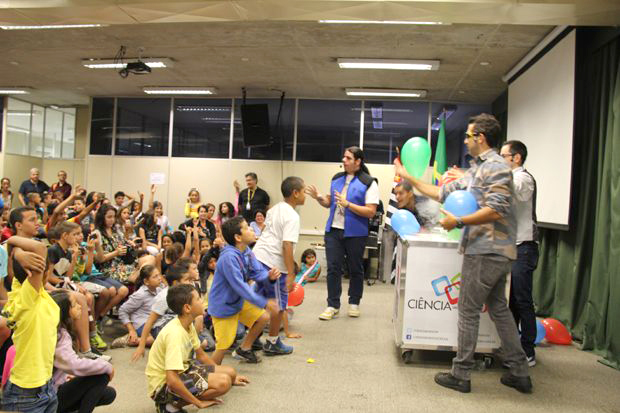
\includegraphics[width=1.0\linewidth]{../../imagens/Evento-Ciencia-Em-Show.jpg}
                \caption{Evento cient\'{i}fico e cultural do WASH, realizado no CTI Renato Archer, em 11 de abril de 2015, com a participa\c{c}\~ao do Ci\^encia em Show. O car\'ater amplo do evento n\~ao permitiu controlar a presen\c{c}a de participantes que p\^ode ser estimada em perto de duas centenas de crian\c{c}as. (acervo da autora).}
                \label{5340059e38852932c32c5ce8624858fef8a1f3f0}
\end{minipage}%
\hspace{0.5cm}
\begin{minipage}[b]{0.4\linewidth}
        \centering
                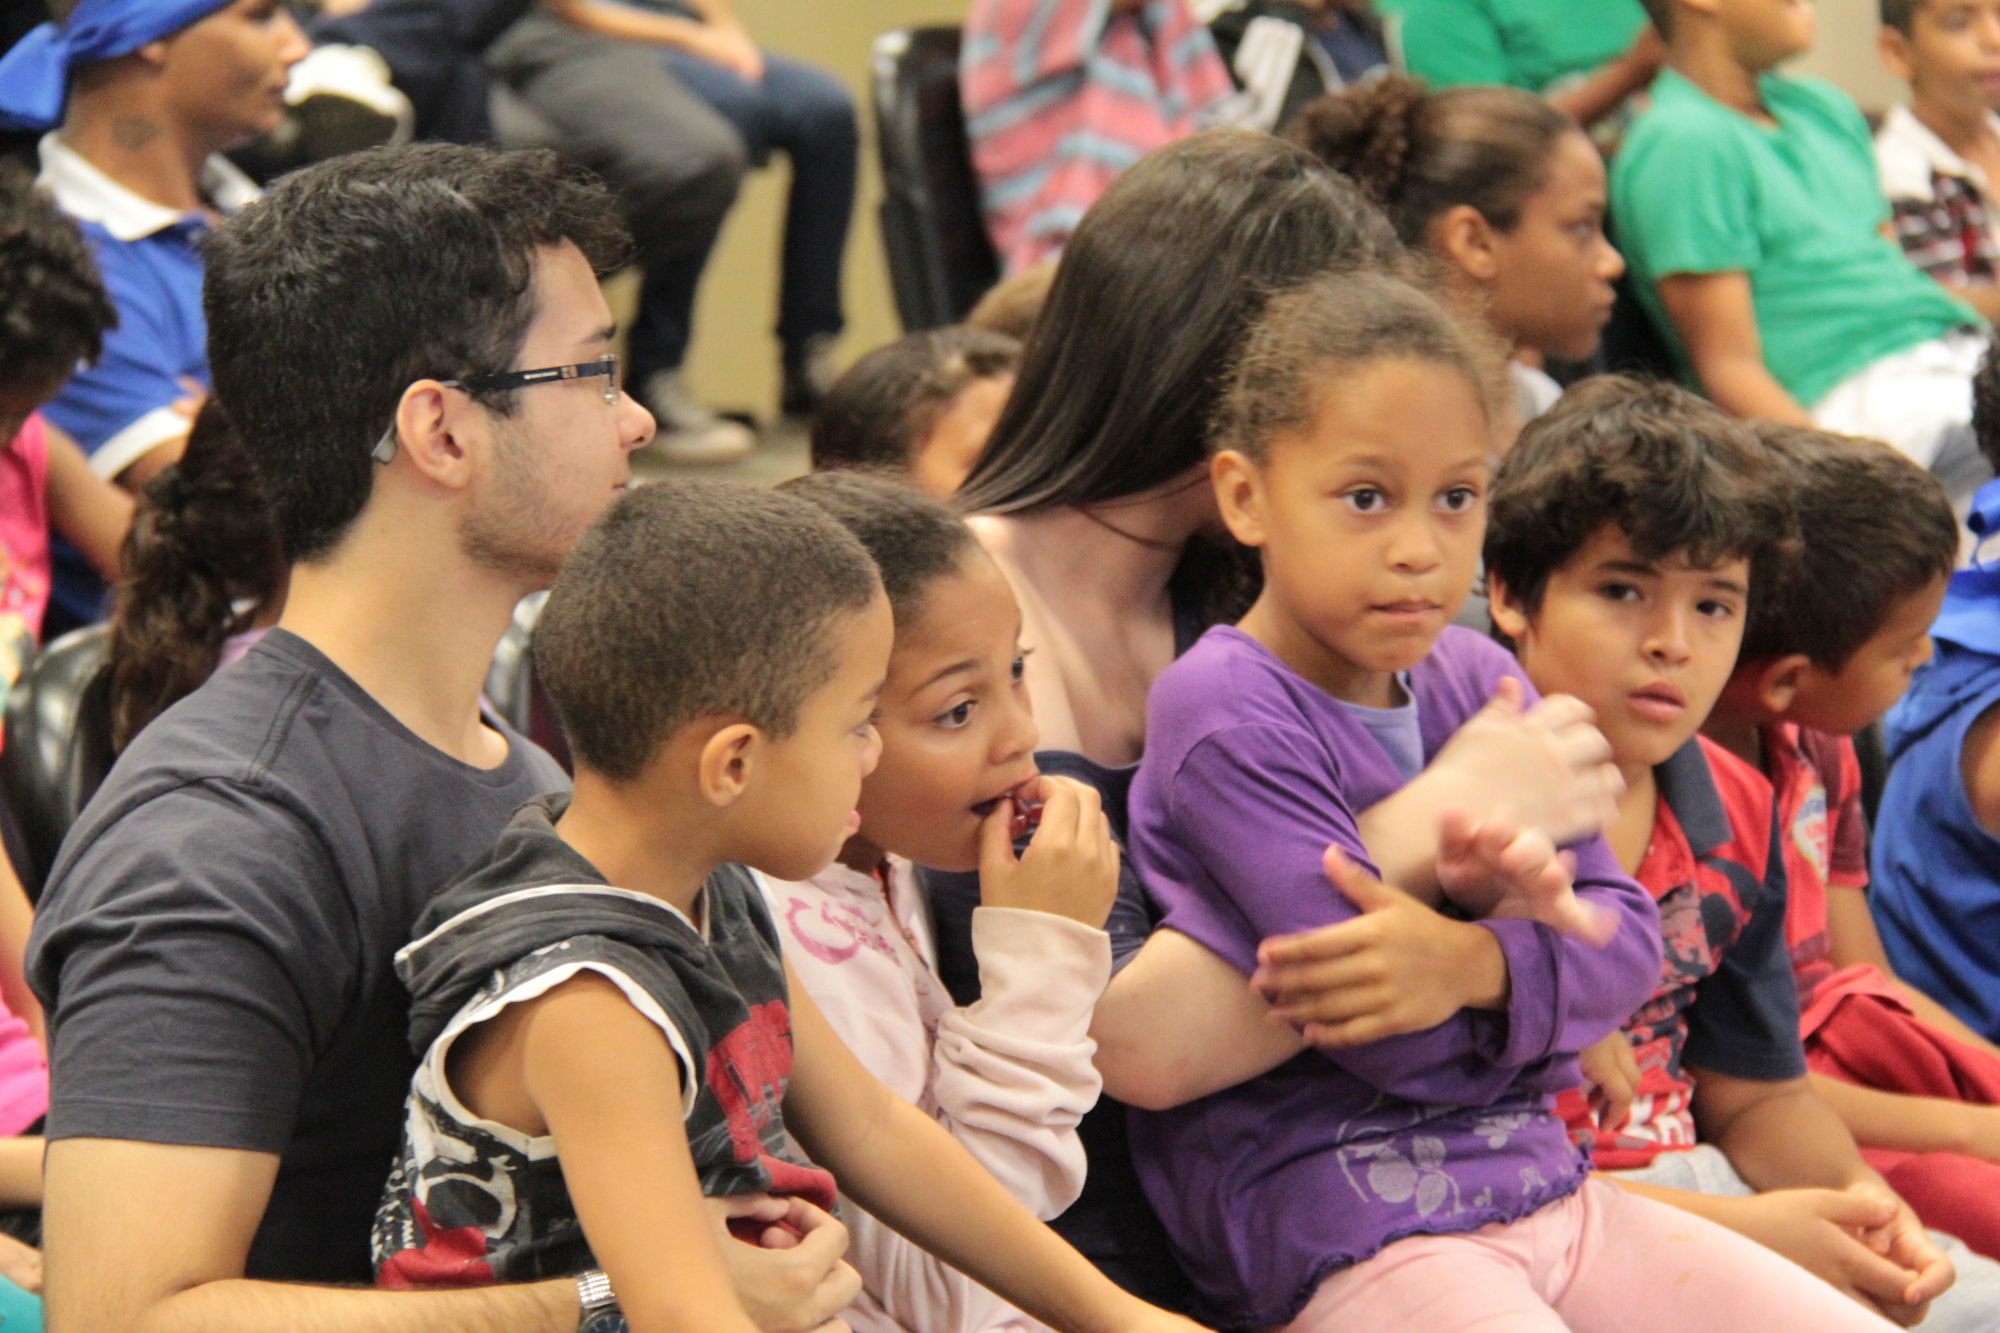
\includegraphics[width=1.0\linewidth]{../../imagens/dia-das-criancas-2022-10-03-menor.JPG}
                \caption{Evento de comemora\c{c}\~ao do dia das crian\c{c}as, com atividades musicais e culturais. Os registros da plataforma apontam para 9 participantes, mas os registros fotogr\'aficos indicam uma presen\c{c}a muito maior. (acervo da autora)}
                \label{31e991b69f3aba382518bb571a4e69a720fa8ccb}
\end{minipage}
\hspace{0.5cm}
\begin{minipage}[b]{0.4\linewidth}
        \centering
                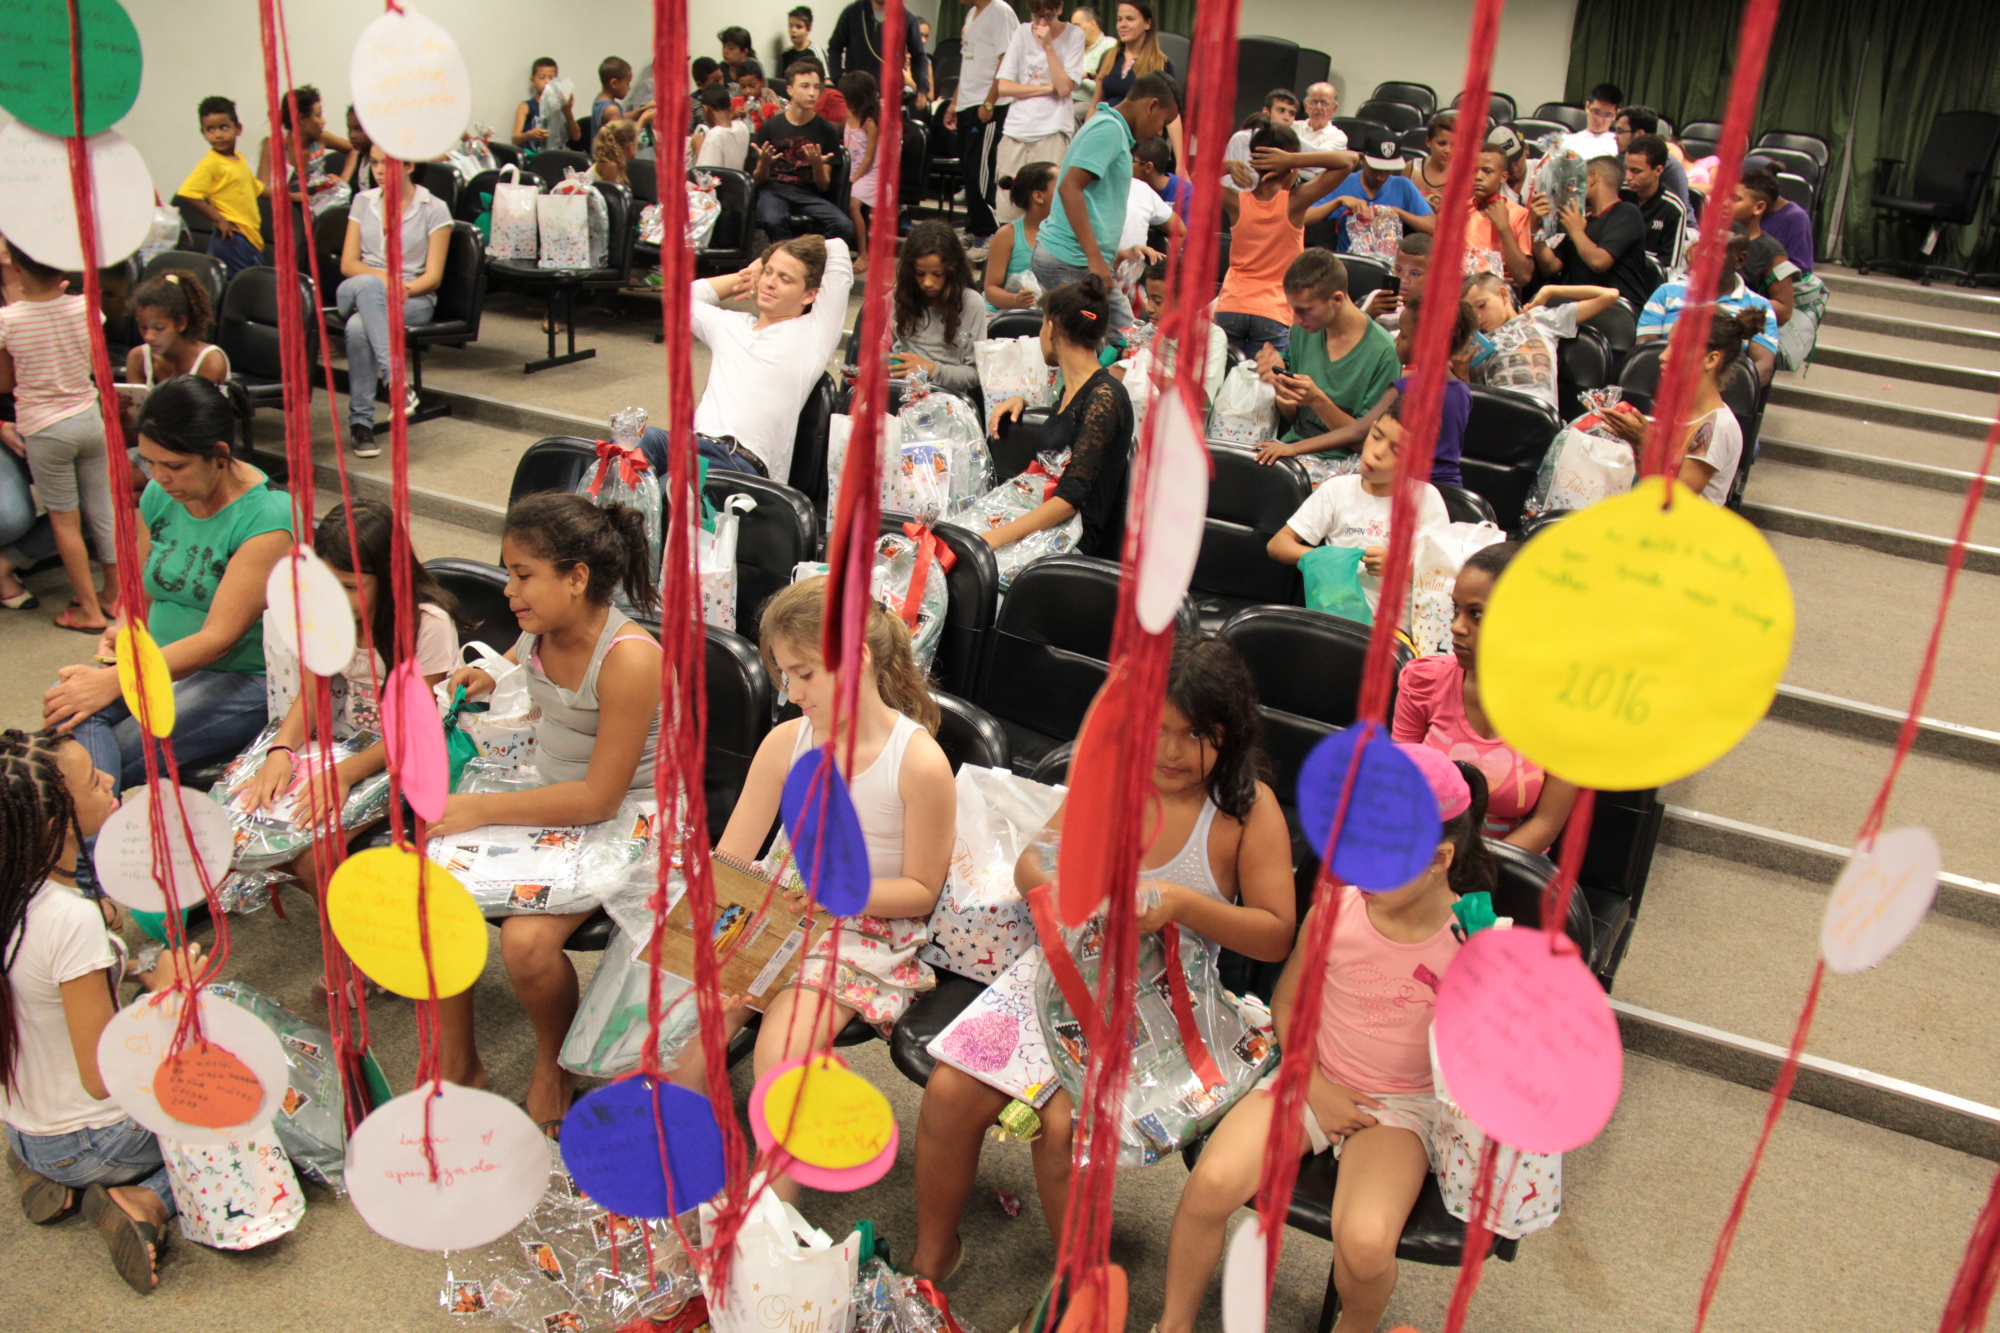
\includegraphics[width=1.0\linewidth]{../../imagens/confraternizacao-de-natal-menor.jpeg}
                \caption{Evento de Natal realizado no CTI Renato Archer, em 19 de dezembro de 2015. O evento incluiu uma variada gama de atividades l\'udicas e educacionais. Muito embora o registro oficial indique a participa\c{c}\~ao de oito pessoas, as fotos mostram que a participa\c{c}\~ao foi muito superior. (acervo da autora)}
                \label{afa1b2acd7f4c590f25d9821e48e82568bd28cf2}
\end{minipage}%
\hspace{0.5cm}
\begin{minipage}[b]{0.4\linewidth}
        \centering
                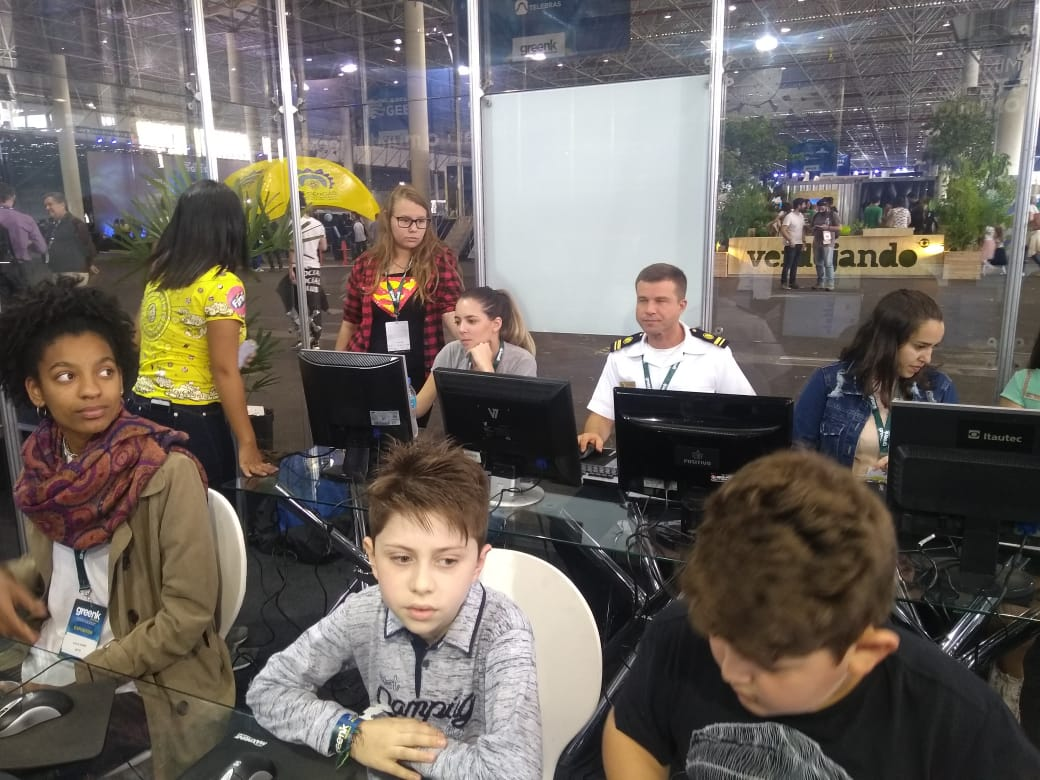
\includegraphics[width=1.0\linewidth]{../../imagens/Evento-Greenk-2018-05-27.jpg}
                \caption{Evento Greenk, patrocinado pelo MCTI, no Expo Center Anhembi em 27 de maio de 2018, que contou com oficinas do WASH. Neste tipo de evento, \'e dif\'{i}cil realizar o cadastro nominal de participantes pela amplitude do mesmo. O p\'ublico beneficiado pode ser estimado em algumas centenas de crian\c{c}as. (acervo da autora).}
                \label{04766cbd557212dbb84969d429be542b364bf87a}
\end{minipage}
\hspace{0.5cm}
\begin{minipage}[b]{0.4\linewidth}
        \centering
                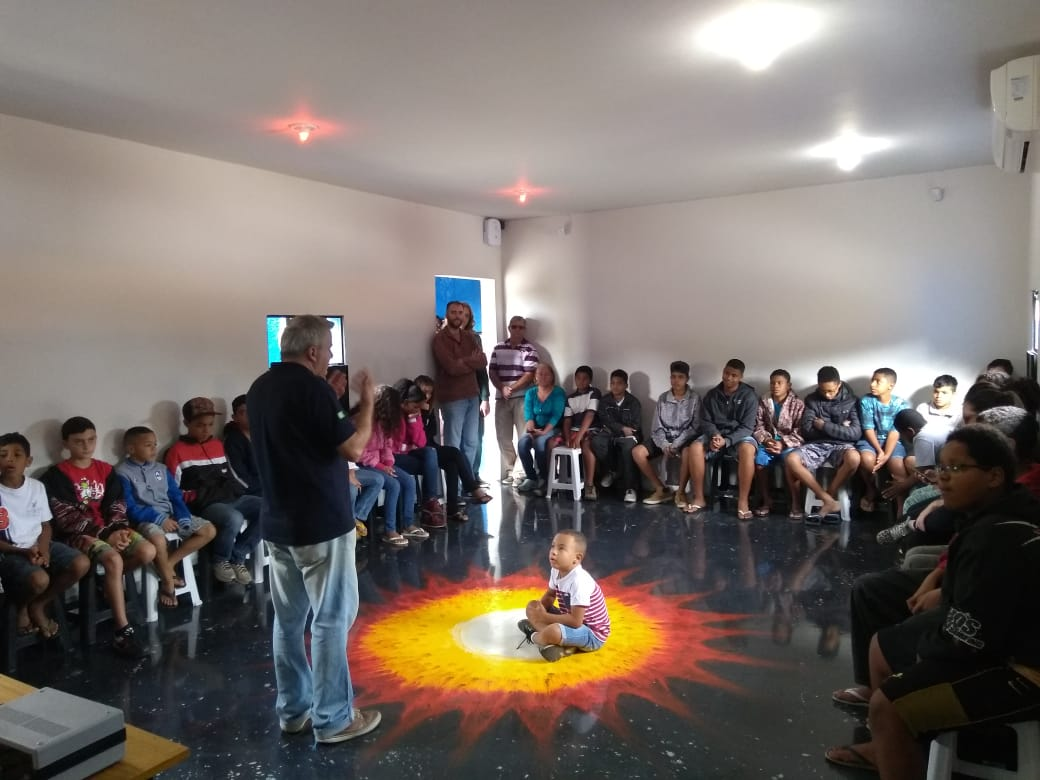
\includegraphics[width=1.0\linewidth]{../../imagens/MAAS.jpg}
                \caption{Evento no Museu Aberto de Astronomia, promovido pelo WASH. Os registros oficiais n\~ao indicam o n\'umero de participantes, mas os registros fotogr\'aficos mostram a participa\c{c}\~ao de dezenas de crian\c{c}as. (acervo da autora)}
                \label{b5542509570e0bcdbabe4949f7fef484141b805e}
\end{minipage}%
\hspace{0.5cm}
\begin{minipage}[b]{0.4\linewidth}
        \centering
                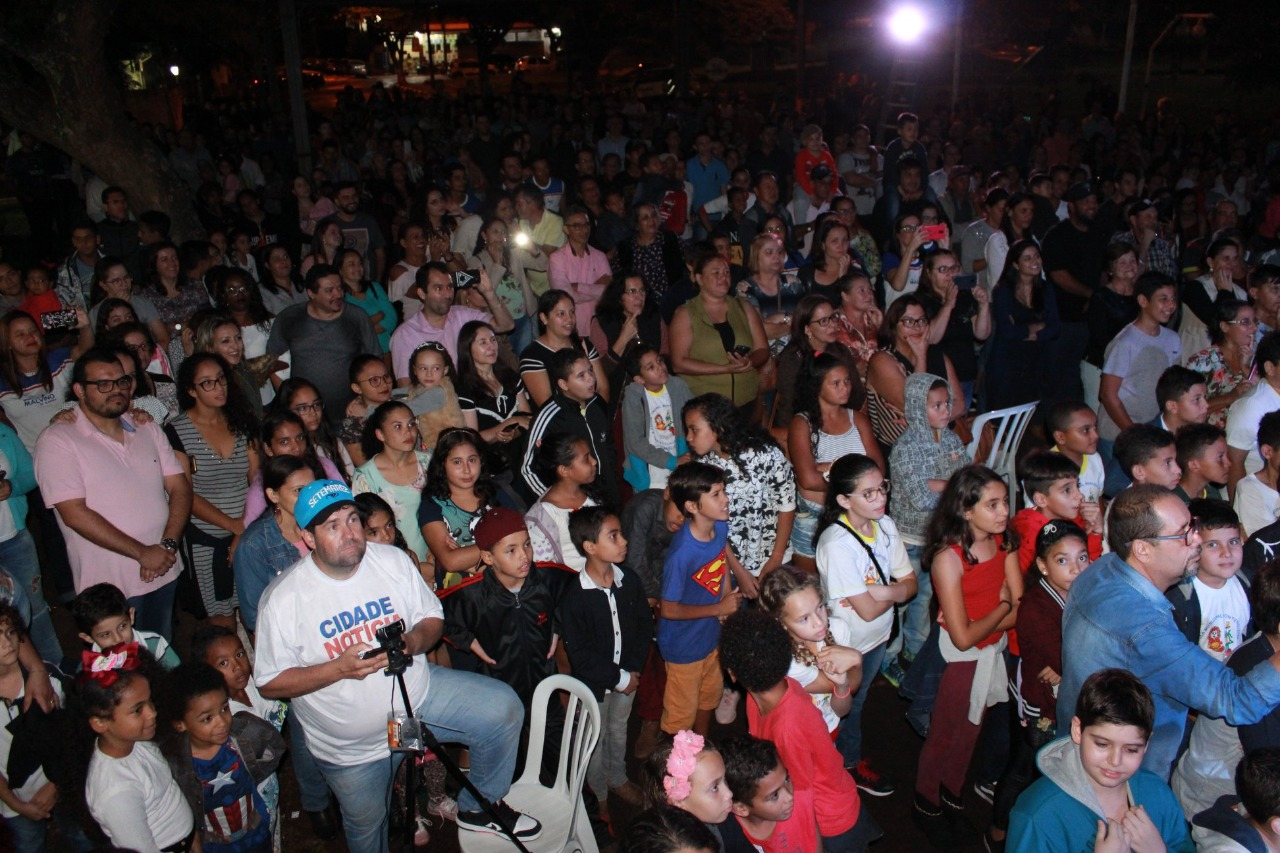
\includegraphics[width=1.0\linewidth]{../../imagens/Ciencia-Prado-publico.jpeg}
                \caption{Evento de demonstra\c{c}\~oes cient\'{i}ficas, na pra\c{c}a de Prado Ferreira, ocorrido em 31 de maio de 2019, onde o WASH realizou dezenas de oficinas. O evento foi promovido pelo WASH no lan\c{c}amento do Programa Profiss\~ao 4.0 e contou com a participa\c{c}\~ao do Ci\^encia em Show, trupe de artistas formados em f\'{i}sica com grande presen\c{c}a na m\'{i}dia televisiva. (acervo da autora)}
                \label{7b56c85cc265fcbf261a3bc788ae1e4619b70725}
\end{minipage}
\hspace{0.5cm}
\end{figure}


















\captionsetup{format=plain}
\begin{figure}[max size={\textwidth}{\textheight}]

\centering


\begin{minipage}[b]{0.4\linewidth}
        \centering
                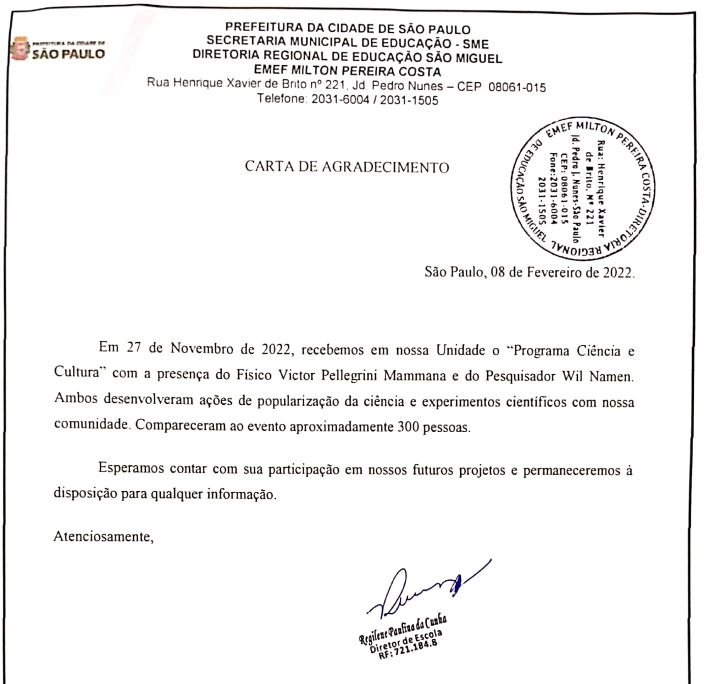
\includegraphics[width=1.0\linewidth]{../../imagens/evento-sao-miguel.png}
                \caption{P\'ublico no evento do Ci\^encia em Show (acervo do Prof. Felipe Can\'e)}
                \label{1005d976e3ba4fdcea3be1ed7501eff18485a145}
\end{minipage}%
\hspace{0.5cm}
\end{figure}



Com os exemplos de eventos at\'e aqui apresentados, buscamos sustentar a afirma\c{c}\~ao de que os 3.265 cadastros de participantes representa uma amostra modesta de todos os benefici\'arios do Programa WASH. Outra evid\^encia que sustenta essa informa\c{c}\~ao \'e o n\'umero de 3.771 eventos realizados, segundo os registros do Recorte B (ver se\c{c}\~ao 3.2). Muito embora ocorra a reten\c{c}\~ao de p\'ublico, com participantes de mais de um evento, a exist\^encia de mais eventos do que participantes recomenda um cuidado maior com a possibilidade de o n\'umero de pessoas benefici\'arias estar subestimado.












N\~ao obstante esse car\'ater amostral, ou seja, incompleto em termos de registros individuais dos participantes, sustentamos que essa amostra \'e adequada para extrair importantes informa\c{c}\~oes sobre o Programa. Entre elas est\'a o seu crescimento anual, o impacto da pandemia e o perfil et\'ario do p\'ublico alvo, por exemplo, o que pode ser verificado nas se\c{c}\~oes a seguir.












\subsection[Evolu\c{c}\~ao temporal do n\'umero de participa\c{c}\~oes]{Evolu\c{c}\~ao temporal do n\'umero de participa\c{c}\~oes}\label{Evolu\c{c}\~ao temporal do n\'umero de participa\c{c}\~oes}
Mesmo n\~ao representando o universo completo de participantes, os dados amostrais s\~ao importantes para identificar tend\^encias do Programa, a exemplo da evolu\c{c}\~ao anual do n\'umero de participa\c{c}\~oes, mostrada na Fig. 37.














\captionsetup{format=plain}
\begin{figure}[max size={\textwidth}{\textheight}]

\centering


\begin{minipage}[b]{0.4\linewidth}
        \centering
                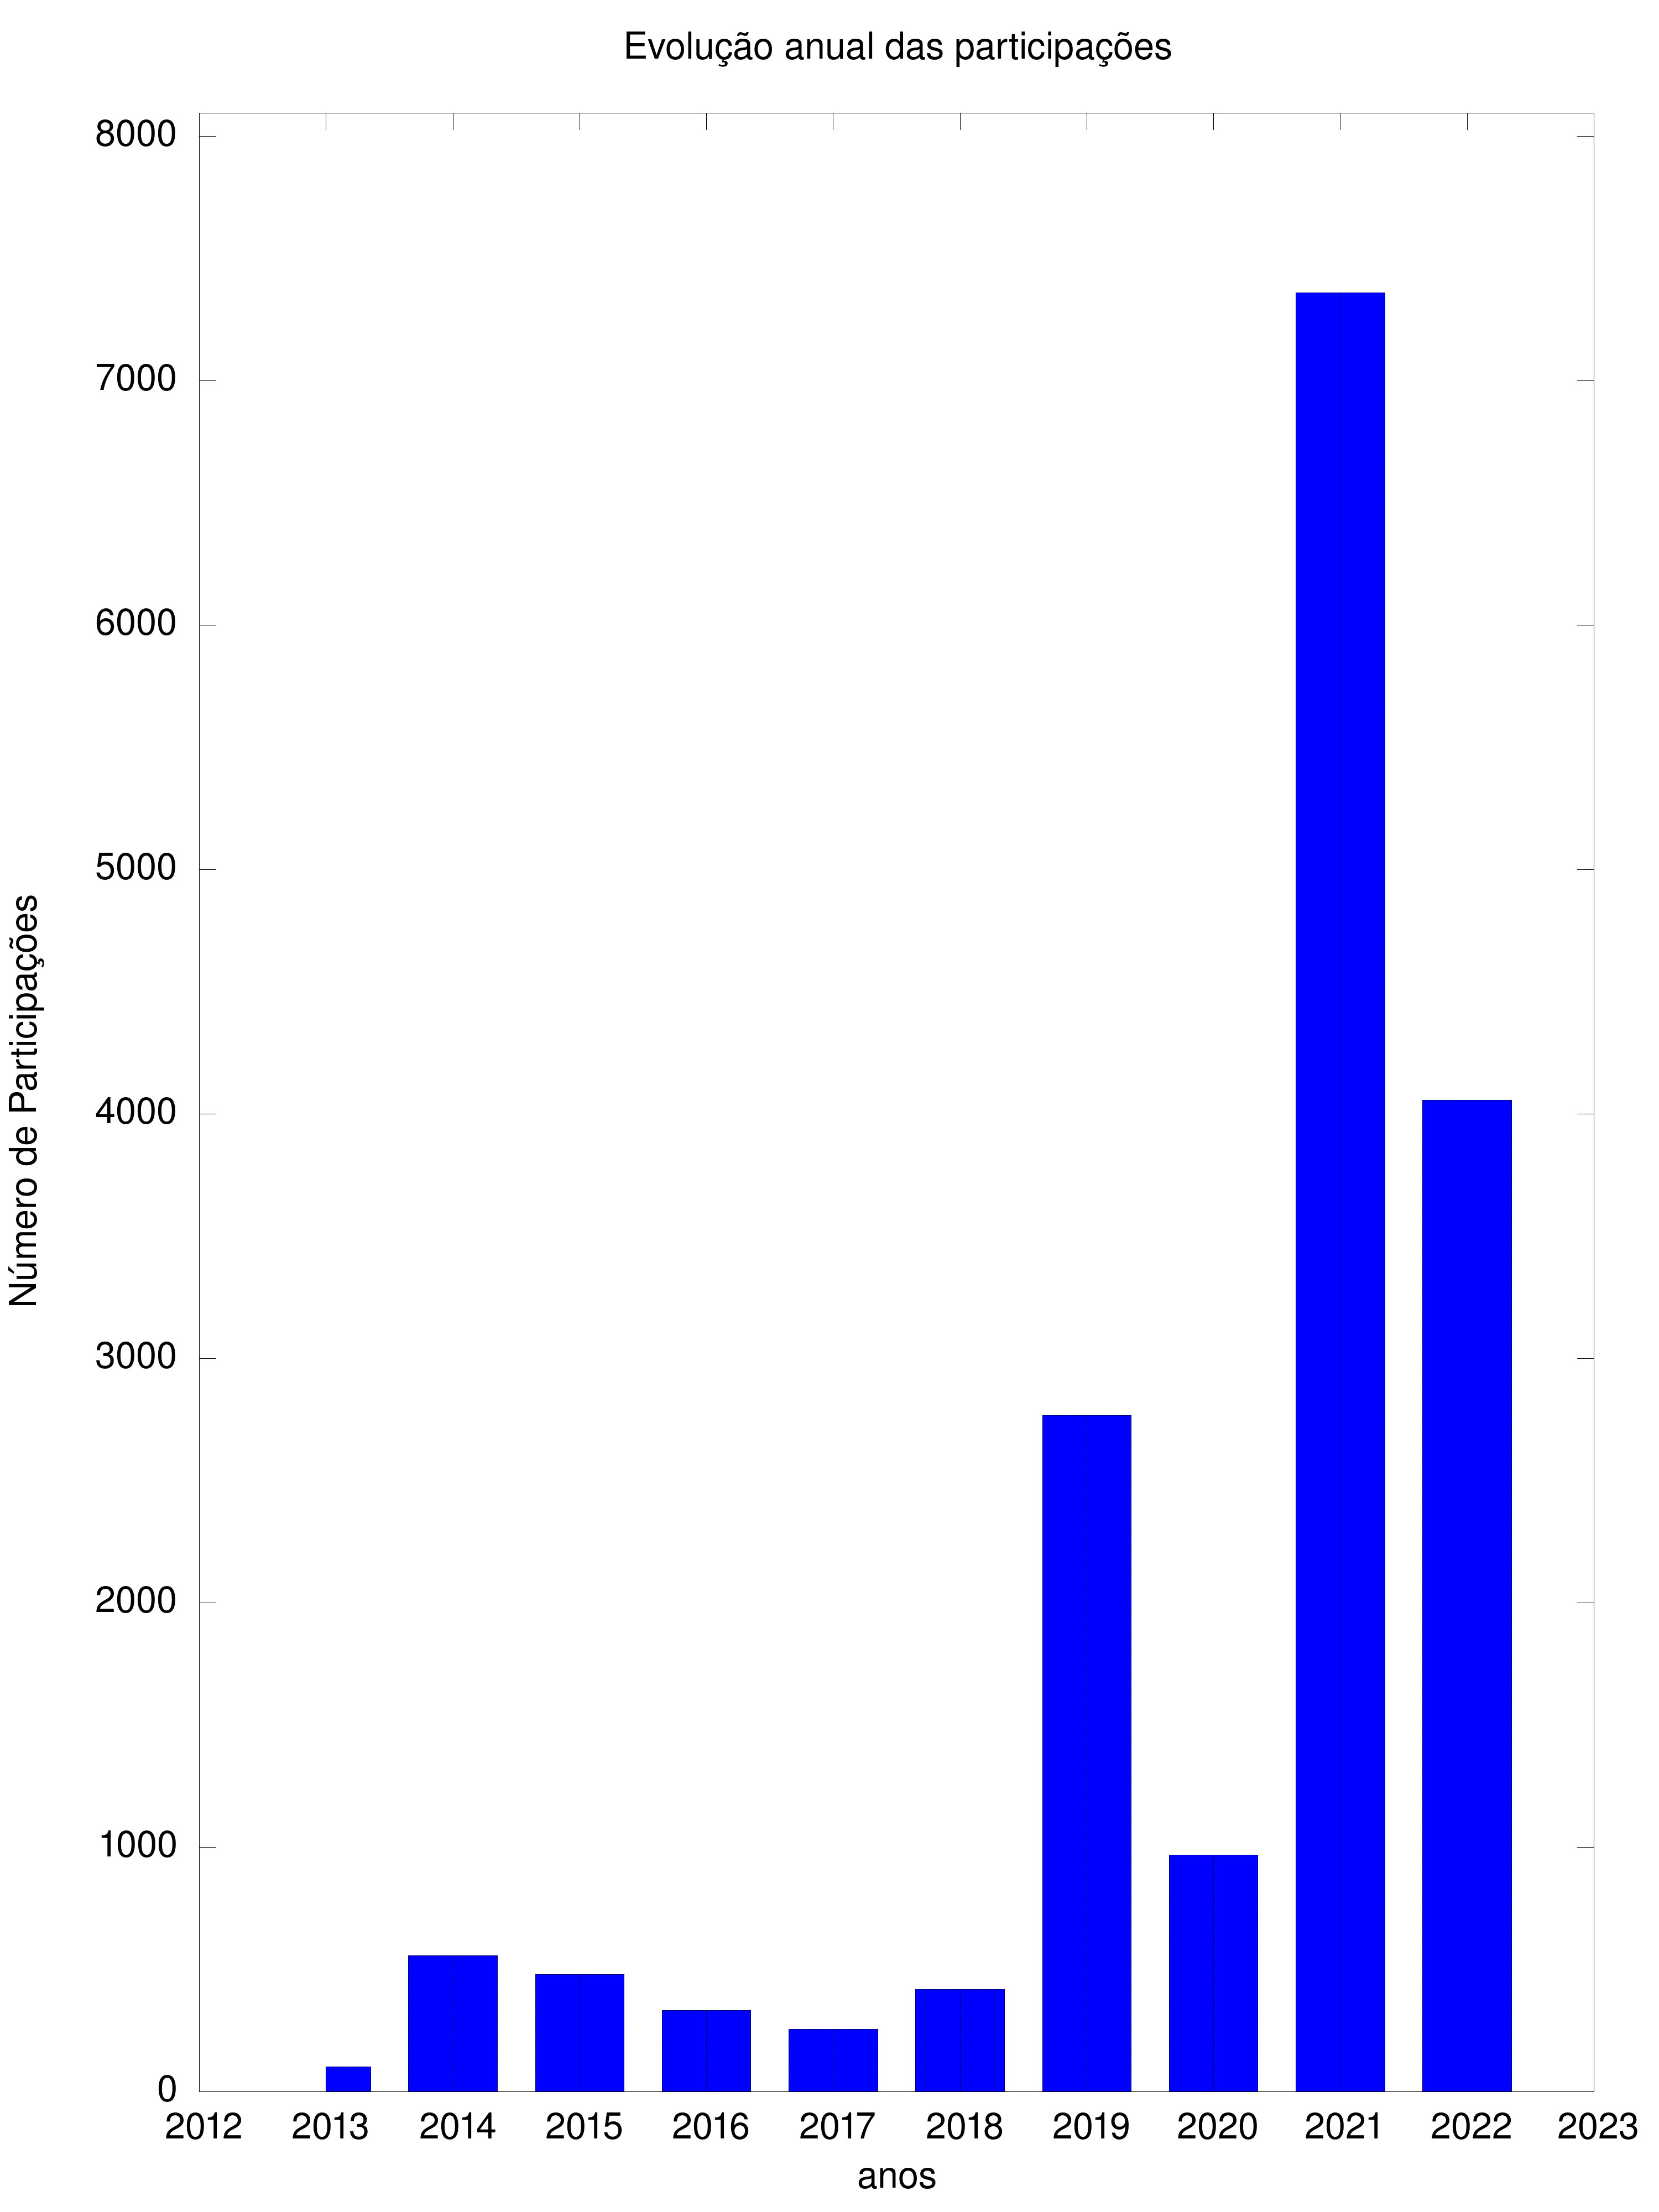
\includegraphics[width=1.0\linewidth]{../../imagens/output-participantes.jpeg}
                \caption{Evolu\c{c}\~ao temporal do n\'umero de participa\c{c}\~oes ao longo dos 10 anos de exist\^encia do Programa WASH, segundo o Recorte A (fonte: elabora\c{c}\~ao pr\'opria).}
                \label{19699bcc5ab8317274249d6743d62534dbfb95fa}
\end{minipage}%
\hspace{0.5cm}
\begin{minipage}[b]{0.4\linewidth}
        \centering
                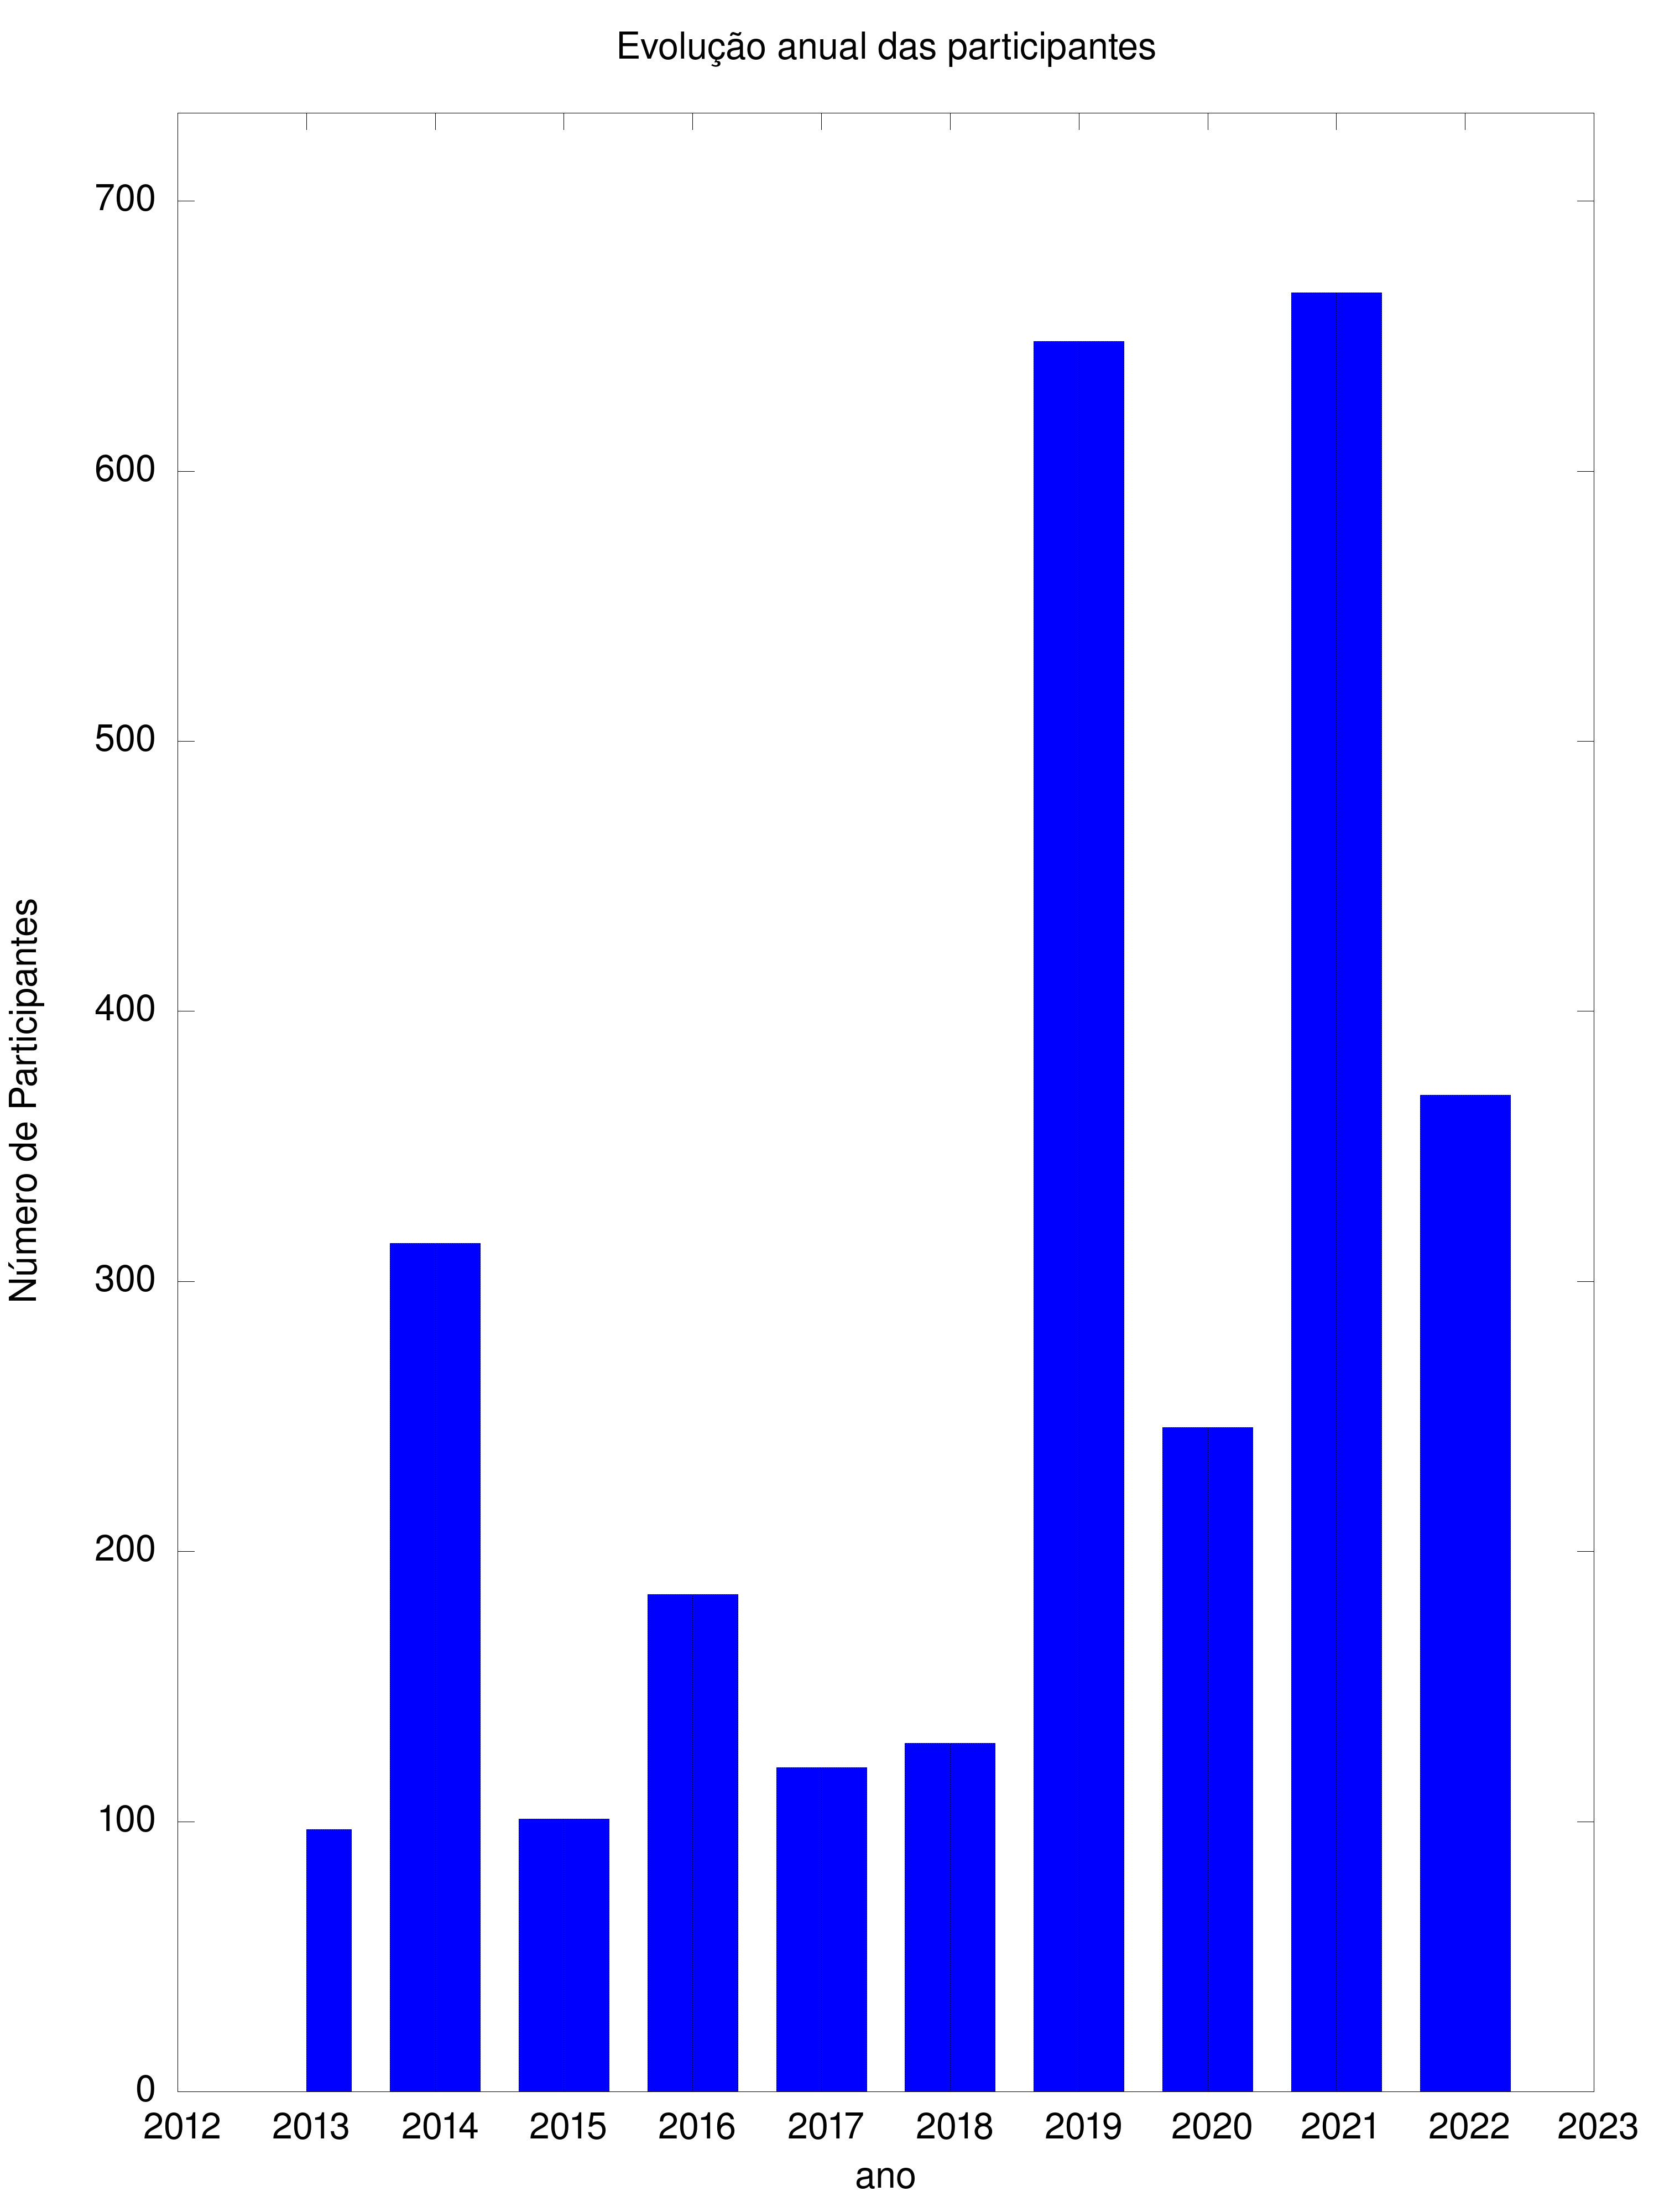
\includegraphics[width=1.0\linewidth]{../../imagens/output-participantes2.jpeg}
                \caption{Evolu\c{c}\~ao anual do n\'umero de participantes individuais segundo o Recorte A (fonte: elabora\c{c}\~ao pr\'opria).}
                \label{e01eb26f443a577db4a1d382417f8c1bb57ee435}
\end{minipage}
\hspace{0.5cm}
\begin{minipage}[b]{0.4\linewidth}
        \centering
                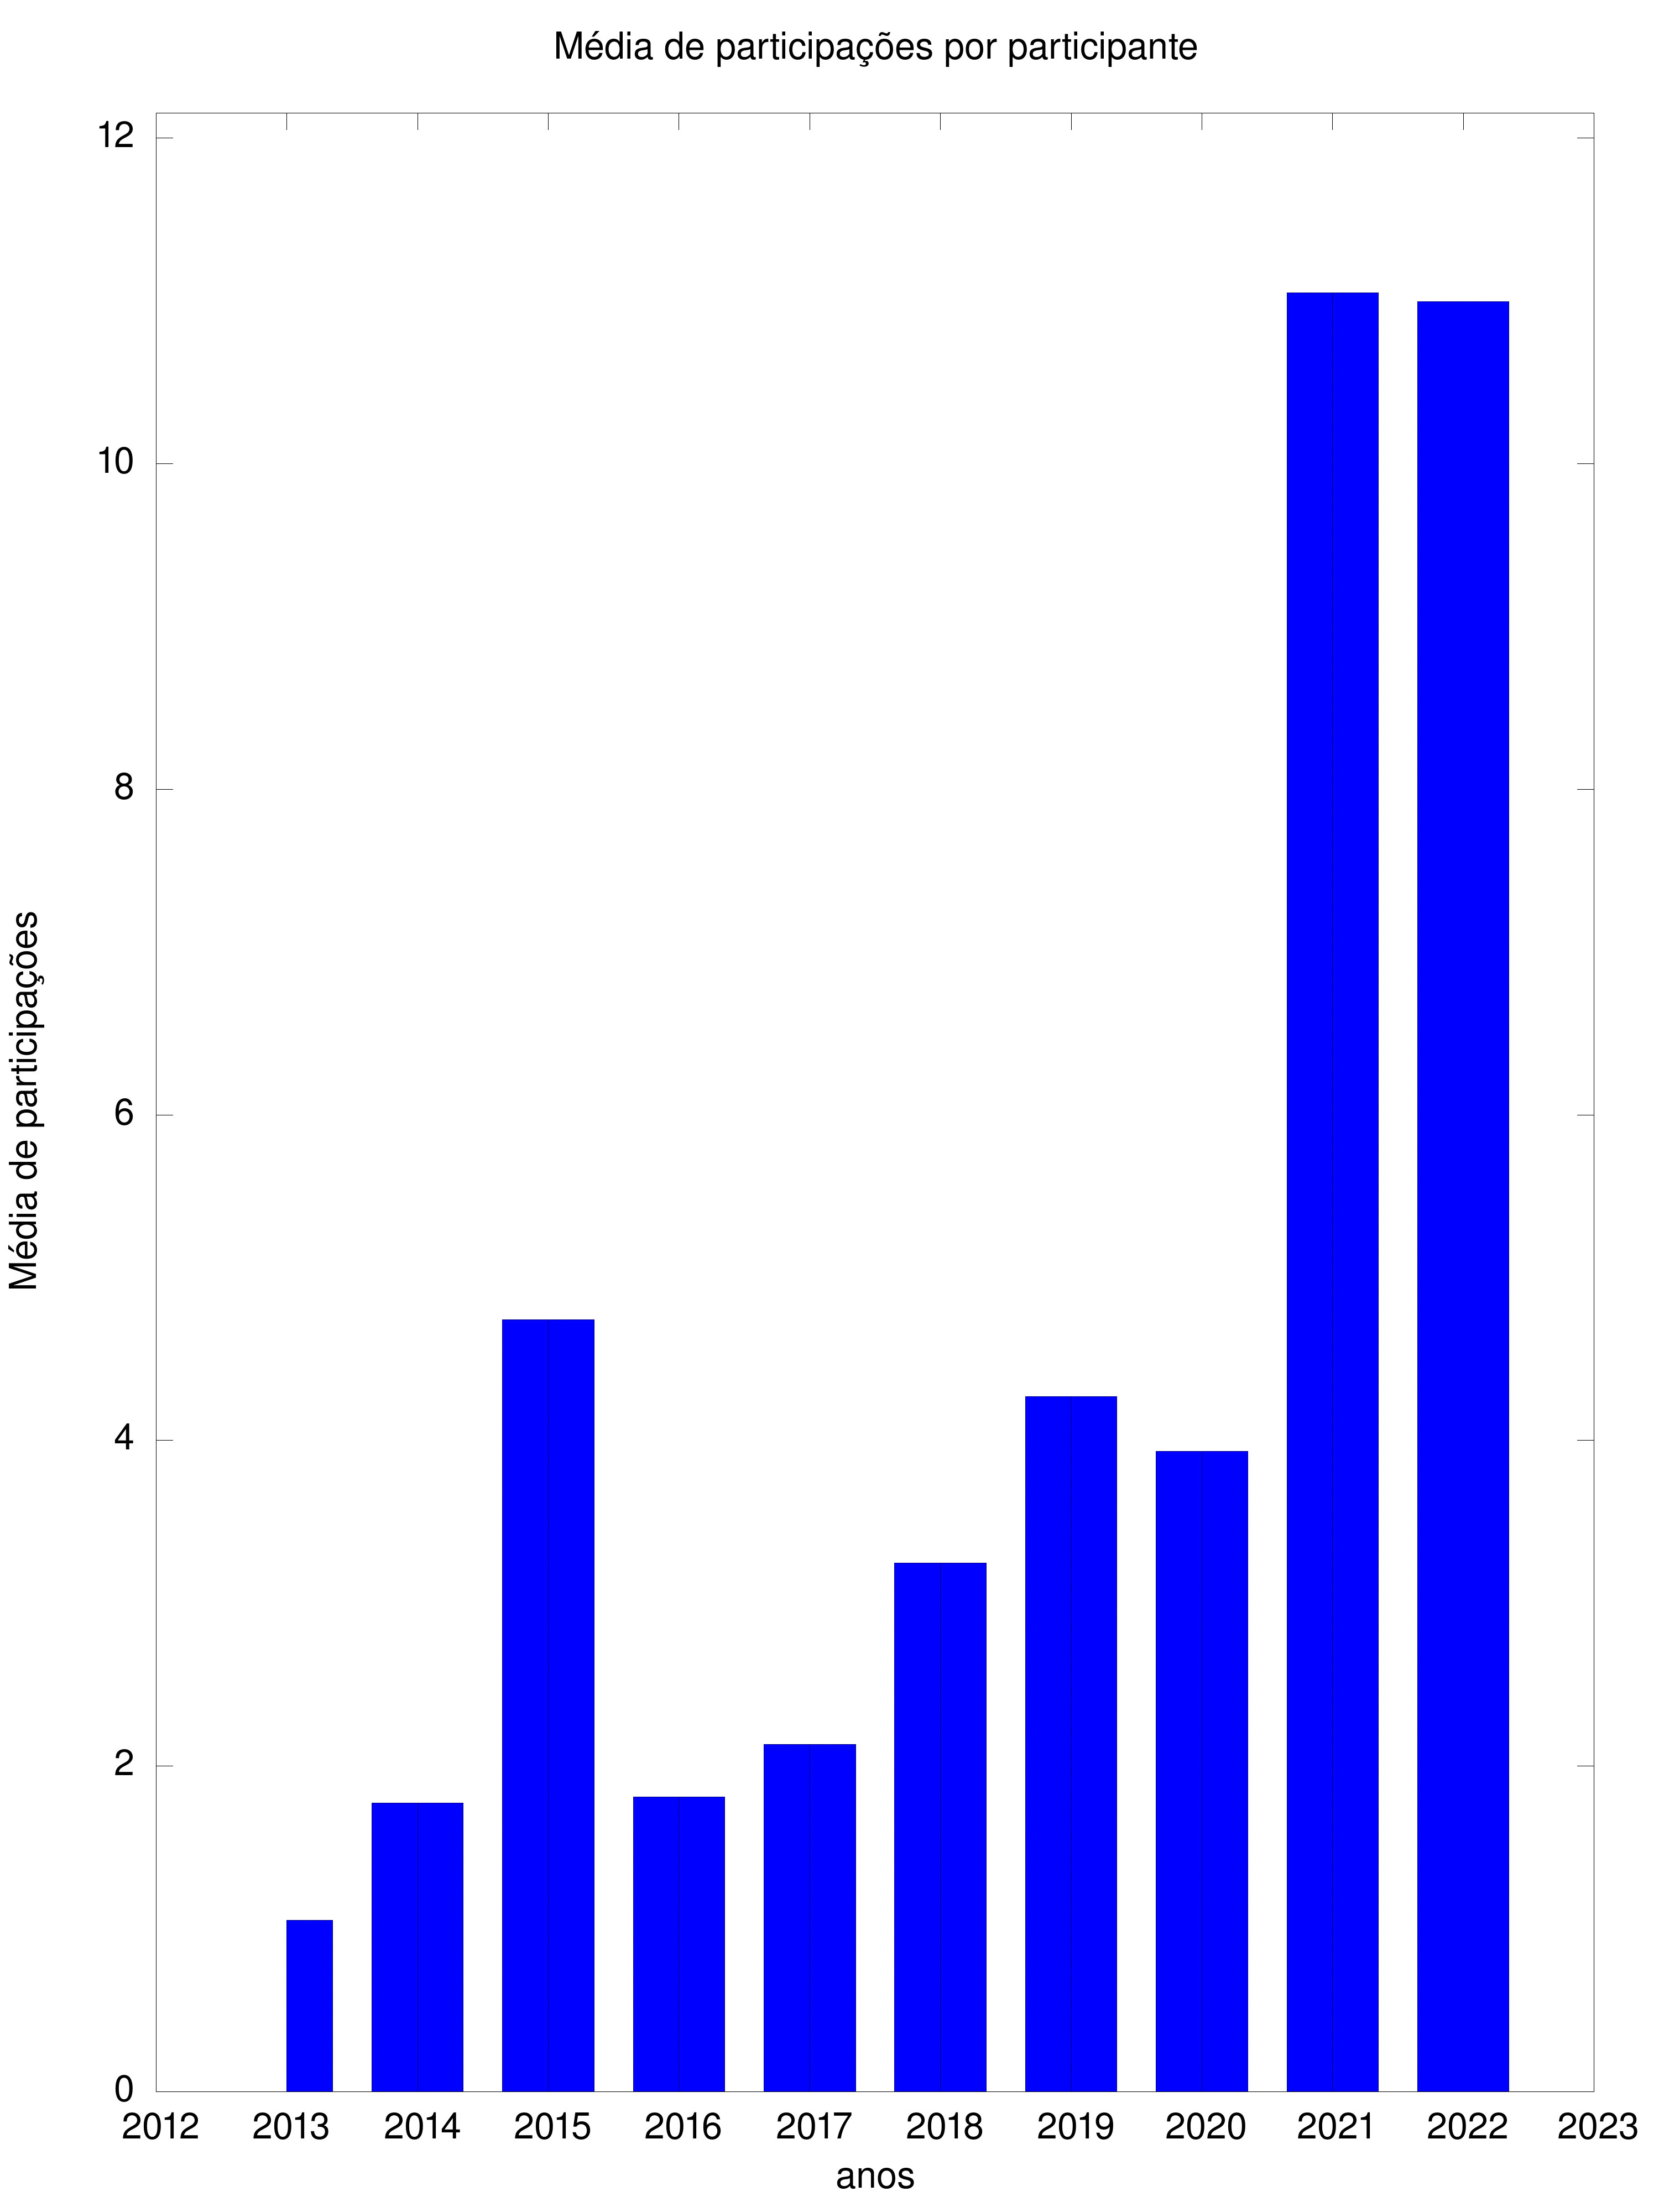
\includegraphics[width=1.0\linewidth]{../../imagens/output-media-participacoes.jpeg}
                \caption{Evolu\c{c}\~ao anual da m\'edia de participa\c{c}\~oes por participante segundo, o Recorte A (fonte: elabora\c{c}\~ao pr\'opria).}
                \label{a8f2d72073b88290f9b8731b144383d2f7c4dc4b}
\end{minipage}%
\hspace{0.5cm}
\end{figure}



\'E importante atentar para uma sutileza: a diferen\c{c}a entre o \textquotedbl\{\} n\'umero de participantes\textquotedbl\{\} e o \textquotedbl\{\}n\'umero de participa\c{c}\~oes\textquotedbl\{\}.












O n\'umero de participa\c{c}\~oes, mostrado na Fig. 37, significa o n\'umero de vezes que participantes frequentaram eventos do WASH naquele ano, ainda que seja contabilizada a mesma pessoa duas ou mais vezes.












O n\'umero de participantes, mostrado na Fig. 38, significa o n\'umero de indiv\'{\i}duos que partiparam de eventos naquele ano, contabilizados uma vez s\'o, ainda que tenham participado em mais de um evento no mesmo ano.












A Fig. 39 mostra a m\'edia de participa\c{c}\~oes por participante, dividindo, um a um, os dados da evolu\c{c}\~ao anual das participa\c{c}\~oes pela evolu\c{c}\~ao anual dos participantes. Como se v\^e no gr\'afico, os dados amostrais indicam um crescimento no n\'umero de \textquotedbl\{\}retornos\textquotedbl\{\} de participantes.












Os gr\'aficos de evolu\c{c}\~ao anual de participa\c{c}\~oes (ver Fig. 37), participantes (ver Fig. 38) e de m\'edia de participa\c{c}\~oes (ver Fig. 39) indicam um crescimento do Programa WASH, principalmente a partir de 2019, ano em que houve tamb\'em um crescimento no n\'umero de emendas parlamentares.












Ao mesmo tempo, os gr\'aficos indicam que a pandemia teve impacto negativo no atendimento de educandos por parte do WASH, uma vez que observou-se uma queda abrupta em 2020, tanto em termos de participa\c{c}\~oes quanto de participantes.












N\~ao obstante a manuten\c{c}\~ao de parte das restri\c{c}\~oes de isolamento social no ano de 2021, os gr\'aficos das Figs. 37 e 38 mostram uma recupera\c{c}\~ao nos indicadores de participantes e participa\c{c}\~oes naquele ano (lembrando que os dados para 2022, no Recorte A, s\~ao parciais). Atribu\'{\i}mos essa recupera\c{c}\~ao \`as medidas tomadas pelo WASH de desenvolver oficinas remotas, mesmo o WASH ter sido concebido como Programa presencial  (CTI, 2018). Essas medidas est\~ao descritas na se\c{c}\~ao 4.1.6.












Esse aprendizado sobre como realizar oficinas remotas precisa se refletir na revis\~ao do Documento de Refer\^encia do WASH, uma vez que o anexo \`a Portaria CTI 178/2018 n\~ao traz qualquer refer\^encia a este m\'etodo.












Finalmente, \'e preciso enfatizar que os dados para 2022 s\~ao parciais, uma vez que a presente an\'alise refere-se a um Recorte A, cujo per\'{\i}odo se encerra em agosto daquele ano.












\subsection[Distribui\c{c}\~ao de partipantes por sexo (equidade)]{Distribui\c{c}\~ao de partipantes por sexo (equidade)}\label{Distribui\c{c}\~ao de partipantes por sexo (equidade)}
As pessoas do sexo feminino s\~ao particularmente desprivilegiadas quando o tema \'e igualdade de acesso \`as disciplinas de Science, Technology, Engineering and Mathematics (Kijima et al., 2021).












Por esta raz\~ao, \'e de muito interesse para este trabalho analisar o equil\'{\i}brio no atendimento a participantes do sexo masculino e do sexo feminino, com vistas a determinar a equidade.












Mas esta an\'alise, como antecipado no cap\'{\i}tulo de Materiais e M\'etodos, n\~ao foi planejada no in\'{\i}cio do Programa.












Portanto, identificamos a necessidade de desenvolver um m\'etodo para estimar o equil\'{\i}brio entre participantes femininos e masculinos, criando um indicador de equidade. Este m\'etodo \'e baseado na contagem dos registros, cujo o primeiro nome do cadastrado est\'a presente numa lista de \textquotedbl\{\}nomes masculinos\textquotedbl\{\}; e na contagem simult\^anea dos registros, cujo o primeiro nome da cadastrada est\'a presente numa lista de \textquotedbl\{\} nomes femininos\textquotedbl\{\} (ver detalhes em Materiais e M\'etodos, se\c{c}\~ao 3.2.4).












Este m\'etodo de \textquotedbl\{\} estimativa \textquotedbl\{\} n\~ao tem a finalidade de atribuir, individualmente, o sexo a cada participante porque n\~ao se deseja estigmatizar os participantes que, por falha de cadastro do Programa, n\~ao tiveram a oportunidade de fazer sua autodeclara\c{c}\~ao de sexo.












A partir de 2019, foi inclu\'{\i}do na plataforma Platu\'oxe um campo autodeclarat\'orio sobre sexo do (a) participante, uma parte dos dados usada para gerar o indicador de equidade foi fornecida pelos (as) pr\'oprios (as) participantes.












O gr\'afico abaixo mostra a distribui\c{c}\~ao dos sexos feminino, masculino,  desconhecido e outros, no universo de participantes do WASH. Nota-se um equil\'{\i}brio entre o n\'umero de participantes, sendo 49.4\%  mulheres e 48.3\% homens, havendo ainda 2.1\% de sexo desconhecido. Apenas cinco cadastros apontam a identidade de g\^enero autodeclarada.












O gr\'afico de \textquotedbl\{\}pizza\textquotedbl\{\} da Fig. 44 mostra a distribui\c{c}\~ao de participantes do sexo masculino e feminino, referindo-se ao universo de participantes cadastrados na Platu\'oxe, de acordo com Recorte A, independentemente do tipo de v\'{\i}nculo. Uma outra informa\c{c}\~ao importante para avaliar a equidade do Programa  WASH \'e a que foi levantada por  FINK (2022), para o per\'{\i}odo de 2020 a 2021, per\'{\i}odo no qual foi poss\'{\i}vel identificar uma significativa preval\^encia de bolsistas do sexo masculino, como indicado na Fig. 41, para uma amostra de 101 bolsistas. Essa amostra refere-se a uma \'unica emenda (Processo CNPq 4000172015-6). Um estudo mais amplo de distribui\c{c}\~ao de bolsas por sexo precisa ser realizado para avaliar se essa tend\^encia continua presente. Do ponto de vista desta disserta\c{c}\~ao, essa situa\c{c}\~ao norteou a revis\~ao do Documento de Refer\^encia, como se ver\'a na se\c{c}\~ao 7.2.














\captionsetup{format=plain}
\begin{figure}[max size={\textwidth}{\textheight}]

\centering


\begin{minipage}[b]{0.4\linewidth}
        \centering
                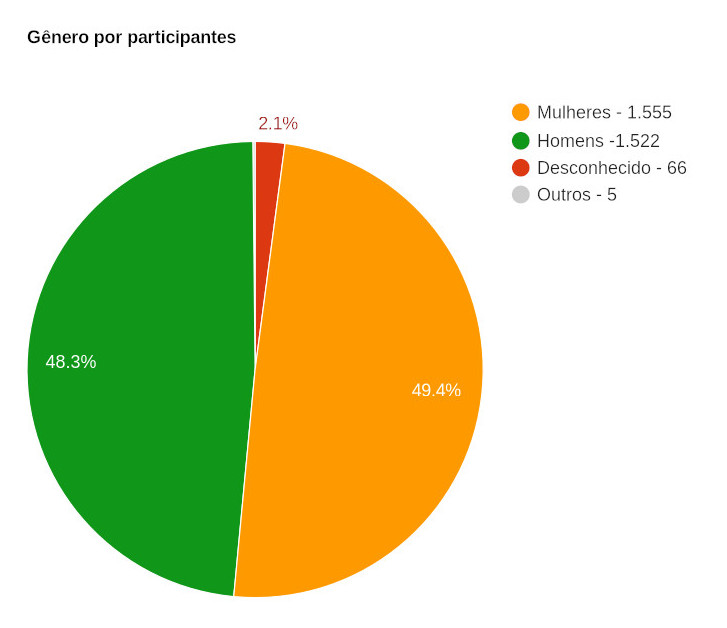
\includegraphics[width=1.0\linewidth]{../../imagens/genero-todos-crop.jpeg}
                \caption{Distribui\c{c}\~ao dos participantes por sexo. Esses dados foram obtidos por meio de infer\^encia, a posteriori, utilizando o primeiro nome dos participantes como forma de estimar o percentual de participantes de ambos os sexos. (fonte: elabora\c{c}\~ao pr\'opria)}
                \label{ef11d820efb73d78fb64eb6bdd03853471a8e89f}
\end{minipage}%
\hspace{0.5cm}
\begin{minipage}[b]{0.4\linewidth}
        \centering
                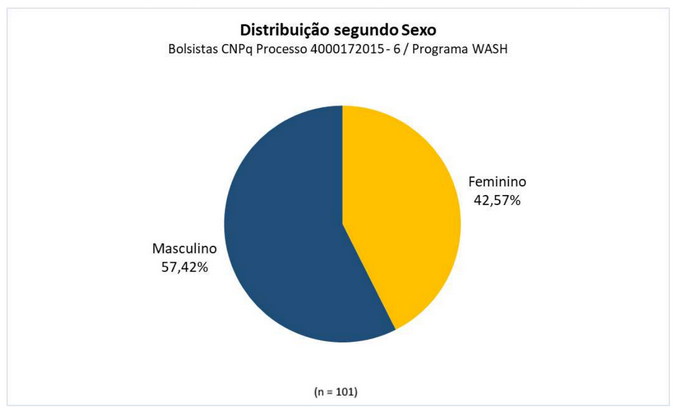
\includegraphics[width=1.0\linewidth]{../../imagens/distribuicao-sexo-bolsistas.png}
                \caption{Distribui\c{c}\~ao de bolsistas por sexo, indicando preval\^encia de bolsistas do sexo masculino para a emenda referente ao Processo CNPq 4000172015-6. O per\'{i}odo de an\'alise foi de 2019 a 2020. (fonte: [[FINK (2022)]])}
                \label{1164a3115bd14e3f25b6b141840652ffbd0d2374}
\end{minipage}
\hspace{0.5cm}
\end{figure}



\subsection[N\'umero de Bolsistas]{N\'umero de Bolsistas}\label{N\'umero de Bolsistas}
O m\'etodo do WASH pressup\~oe a atua\c{c}\~ao de bolsistas de inicia\c{c}\~ao cient\'{\i}fica, extens\~ao e apoio tecnol\'ogico nas seguintes modalidades: ITI A, ITI B, EXP, ATP e ADC, conforme pol\'{\i}tica de Bolsas do CNPq. Os bolsistas realizam suas pesquisas previstas em plano de trabalho, devendo, tamb\'em, atuar como multiplicadores do Programa.












Para determinar o n\'umero de bolsistas no Programa WASH, decidimos utilizar o Recorte B, aplicando consultas estruturadas, de car\'ater mais gen\'erico, na Platu\'oxe, trabalho desenvolvido por Michel Alencar Morandi e publicadas em  WASH (2023).












Para averiguar a abrang\^encia dos dados sobre os (as) bolsistas, no Recorte B da Platu\'oxe, apresentamos a evolu\c{c}\~ao anual de concess\~ao de bolsas, mostrada na Fig. 42.














\captionsetup{format=plain}
\begin{figure}[htb]

	\begin{center}

		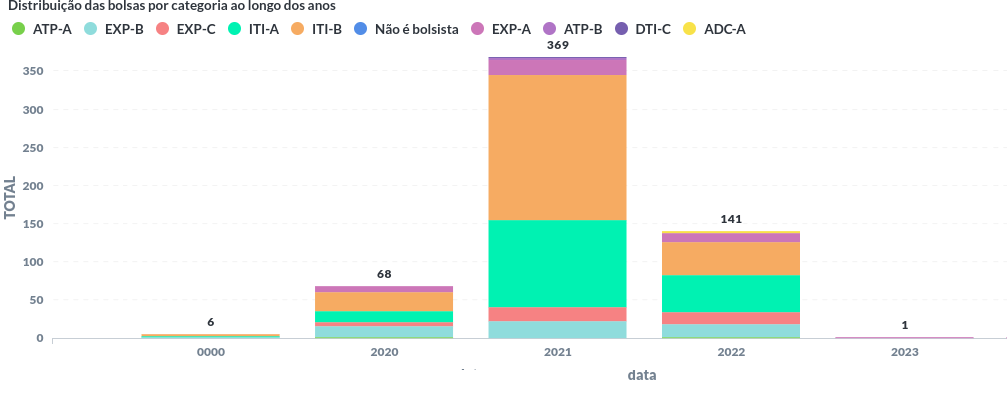
\includegraphics[max size={\textwidth}{\textheight}]{../../imagens/bolsas-anualmente-recorte-b-crop.png}

	\end{center}

	\caption{\label{3f695a85b367790579065c12b40bfa0acdd593f2}Evolu\c{c}\~ao anual de bolsistas do WASH, segundo o Recorte B. As cores indicam modalidades de bolsas. (fonte:  [[WASH (2023)]], por demanda da autora)}

\end{figure}

A Fig. 42, por n\~ao apresentar dados para anos anteriores a 2020, mostra que os dados de bolsistas, presentes no Recorte B da Platu\'oxe n\~ao refletem a totalidade de bolsistas do Programa, mesmo que o Recorte B se refira a um per\'{\i}odo iniciado em setembro de 2013. Em outras palavras, a Fig. 42 mostra que na Platu\'oxe est\~ao registradas apenas bolsas iniciadas  em 2020, 2021 e 2022. Isso ocorre porque o armazenamento dos dados de bolsistas n\~ao fazia parte da vers\~ao original da Platu\'osh, que passou a ter esse recurso apenas a partir de 2019-2020. A barra com legenda \textquotedbl\{\}0000\textquotedbl\{\} indica que h\'a dados esp\'urios na amostra, os quais devem ser desconsiderados (\textquotedbl\{\}0000\textquotedbl\{\} indica que o ano de concess\~ao da bolsa registrada na Platu\'oxe \'e desconhecido).












A interpreta\c{c}\~ao do gr\'afico da Fig. 42 requer um cuidado: ele n\~ao mostra as bolsas vigentes, mas iniciadas em determinado ano. Portanto, a barra para o ano de 2022, por exemplo, pode dar a ideia err\^onea de que houve uma redu\c{c}\~ao de bolsistas naquele ano, mas, a rigor, h\'a bolsas iniciadas em 2021 que ainda podem estar vigentes em 2022. Nesse caso, o n\'umero de bolsistas vigentes em 2022 seria maior do que o n\'umero de bolsas iniciadas em 2022.












Apesar da limita\c{c}\~ao do Recorte B que traz dados de bolsistas limitados aos anos de 2020 a 2023, ainda assim \'e poss\'{\i}vel desenvolver an\'alises de utilidade para essa disserta\c{c}\~ao. Mas, n\~ao se deve perder de vista que essas an\'alises s\~ao de car\'ater amostral.












A Fig. 43 mostra a distribui\c{c}\~ao de modalidades de bolsas do WASH, concedidas a partir de 2020 (subconjunto do Recorte B).














\captionsetup{format=plain}
\begin{figure}[htb]

	\begin{center}

		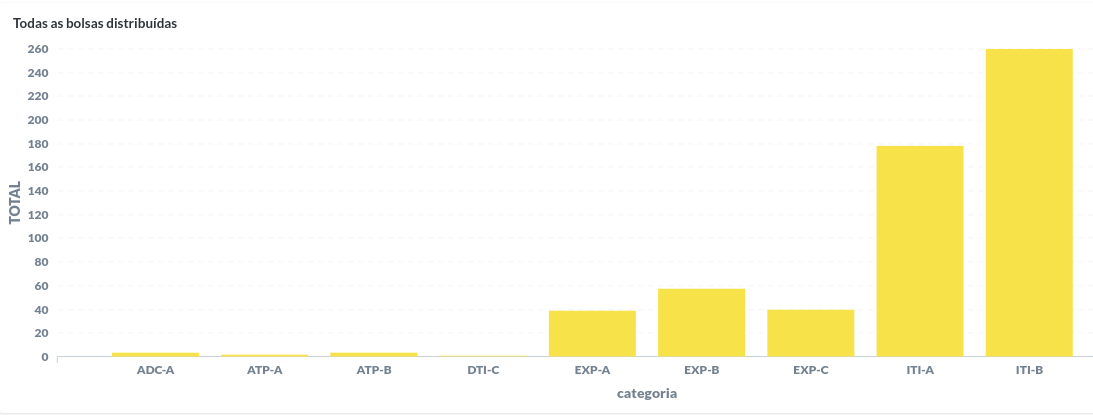
\includegraphics[max size={\textwidth}{\textheight}]{../../imagens/quantidade-bolsistas-3.png}

	\end{center}

	\caption{\label{27e98d39e299354bc7619996ee91fe3d2cf0e56c}Distribui\c{c}\~ao de tipos de bolsas no Programa WASH. (fonte: [[WASH (2023)]], por demanda da autora)}

\end{figure}

Os dados do gr\'afico da Fig. 43 podem ser vistos na Tabela 11.












A Tabela 11 mostra que 75\% das bolsas do WASH, concedidas entre 2020 e 2023 (Recorte B), s\~ao dedicadas para a inicia\c{c}\~ao cient\'{\i}fica (ITI A e ITI B). Isso \'e um indicativo de que o p\'ublico alvo do Programa, definido pela Portaria CTI 178/2018, tem sido priorizado, dado que s\~ao os bolsistas de inicia\c{c}\~ao cient\'{\i}fica que desempenham o papel de multiplica\c{c}\~ao junto aos educandos das redes de ensino e de outras entidades respons\'aveis. De fato, a Portaria CTI 178/2018 prev\^e:













\noindent\begin{center}\mbox{\centering\fbox{\centering\par\parbox{0.7\linewidth}{\small\textit{\textquotedbl\{\}O p\'ublico alvo das oficinas deve ser constitu\'{\i}do preponderantemente de estudantes do ensino fundamental, mas adolescentes e adultos tamb\'em podem participar, a exemplo dos pais dos educandos, os quais s\~ao sempre convidados.\textquotedbl\{\} (fonte: Portaria CTI 178/2018).}\normalsize}}}\end{center}






\begin{table}[htb]
\tiny
\caption{\label{2422b7c7fe35ecc5010472438083776a7ed64d61}Distribui\c{c}\~ao de bolsas por modalidade no Recorte B da Platu\'oxe, ressalvando que, nesse recorte, h\'a apenas dados das bolsas concedidas a partir de 2020. (fonte:  [[WASH (2023)]], por demanda da autora).}

\centering
\begin{tabular}{|c|c|c|}
\hline
modalidade de Bolsa  &  tipo  &  quantidade \\
\hline
ITI A  &  inicia\c{c}\~ao  &  178 \\
ITI B  &  inicia\c{c}\~ao  &  260 \\
EXP A  &  extens\~ao  &  39 \\
EXP B  &  extens\~ao  &  57 \\
EXP C  &  extens\~ao  &  40 \\
ATP A  &  extens\~ao  &  2 \\
ATP B  &  extens\~ao  &  3 \\
ADC A  &  difus\~ao  &  3 \\
DTI C  &  desenvolvimento  &  1 \\
\hline
  &  TOTAL  &  583 \\
\hline
\end{tabular}
\end{table}


Outro aspecto no Recorte B \'e a preval\^encia de bolsas de inicia\c{c}\~ao para estudantes do ensino m\'edio, uma \^enfase que est\'a tacitamente presente no Documento de Refer\^encia do WASH.













\noindent\begin{center}\mbox{\centering\fbox{\centering\par\parbox{0.7\linewidth}{\small\textit{\textquotedbl\{\}Os monitores/bolsistas devem ser estudantes do ensino m\'edio que, como forma de est\'{\i}mulo, recebam bolsas de inicia\c{c}\~ao cient\'{\i}fica. Tamb\'em, s\~ao aceitos como monitores/bolsistas os alunos do ensino superior, desde que beneficiados por bolsas de inicia\c{c}\~ao cient\'{\i}fica compat\'{\i}veis.\textquotedbl\{\} (fonte: Portaria CTI 178/2018)}\normalsize}}}\end{center}


Essa preval\^encia do ensino m\'edio \'e diferencial em rela\c{c}\~ao a outros programas de inicia\c{c}\~ao cient\'{\i}fica da academia, que focalizam a inicia\c{c}\~ao cient\'{\i}fica a partir do ensino superior.












Al\'em das an\'alises pertinentes ao Recorte B, \'e poss\'{\i}vel complementar a caracteriza\c{c}\~ao da concess\~ao de bolsas pelo WASH atrav\'es da an\'alise do Recorte C. Este recorte refere-se aos dados presentes na ferramenta de planejamento do WASH, cujos dados est\~ao limitados a 2020 e 2021. Mesmo com essa limita\c{c}\~ao, que d\'a um car\'ater amostral \`a an\'alise, o Recorte C permite conhecer o histograma de dura\c{c}\~ao das bolsas de inicia\c{c}\~ao cient\'{\i}fica do WASH, uma vez que armazena os per\'{\i}odos de vig\^encia das bolsas, marcando in\'{\i}cio e fim para cada bolsista. Outra caracter\'{\i}stica da ferramenta do Recorte C \'e que ela agrega a dura\c{c}\~ao da bolsa de um bolsista, mesmo quando esta \'e renovada diversas vezes, evitando a contabiliza\c{c}\~ao isolada de trechos de bolsas de um mesmo bolsista no histograma.












A Fig. 44 mostra o histograma de dura\c{c}\~ao das bolsas de inicia\c{c}\~ao cient\'{\i}fica (ITI A e B), agregando-as mesmo quando s\~ao interrompidas e renovadas. Sem esse cuidado, o histograma revelaria o tempo da vig\^encia das bolsas e n\~ao o tempo que um bolsista se vincula ao WASH.














\captionsetup{format=plain}
\begin{figure}[htb]

	\begin{center}

		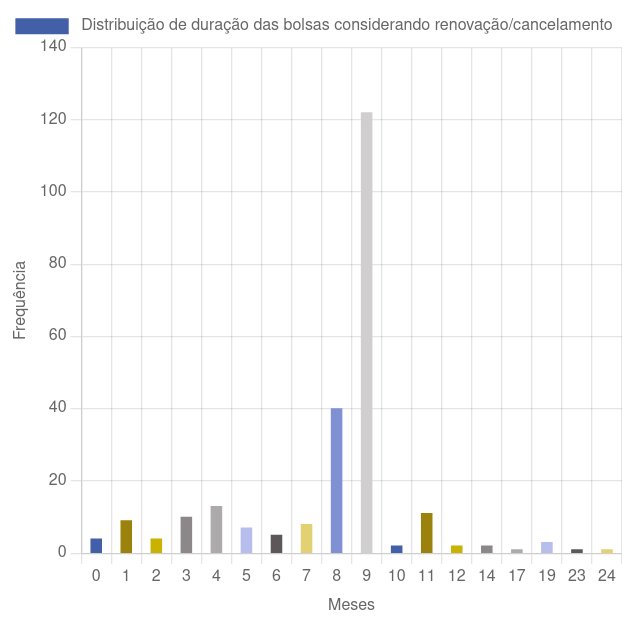
\includegraphics[max size={\textwidth}{\textheight}]{../../imagens/duracao-bolsas.png}

	\end{center}

	\caption{\label{57dff672d55e14e1a107d4c7f63ccc2759fb6b3a}Histograma de dura\c{c}\~ao das bolsas de inicia\c{c}\~ao cient\'{i}fica (ITI A e ITI B) para o Recorte C, pertinente ao per\'{i}odo de 2020 a 2021. (fonte: coordena\c{c}\~ao do Projeto WASH, com a participa\c{c}\~ao da autora)}

\end{figure}

O histograma da Fig. 44 indica que, para o per\'{\i}odo de 2020 a 2021, houve uma preval\^encia de vincula\c{c}\~ao de bolsistas de inicia\c{c}\~ao com dura\c{c}\~ao de nove meses, um tempo compat\'{\i}vel com o per\'{\i}odo letivo. O gr\'afico mostra, tamb\'em, que muitas bolsas se encerram com poucos meses de concess\~ao, indicando a ocorr\^encia de \textquotedbl\{\}turn-over\textquotedbl\{\}, ou seja, uma relevante rotatividade de bolsistas. Essa situa\c{c}\~ao \'e normalmente observada no n\'{\i}vel de inicia\c{c}\~ao cient\'{\i}fica, talvez um resultado das incertezas da adolesc\^encia, quando ainda n\~ao est\~ao consolidados os interesses profissionais.












Por outro lado, observam-se na Fig. 44 dados que indicam que h\'a estudantes que ficam por mais de um ano como bolsistas do WASH, embora isso ocorra com menor incid\^encia.












A amostra de bolsas de inicia\c{c}\~ao cient\'{\i}fica (438), mesmo limitada para o per\'{\i}odo de 2020 a 2023, coloca o WASH entre os maiores Programas do g\^enero no Brasil, inclusive quando essa quantidade \'e comparada com a de grandes universidades p\'ublicas brasileiras.












A experi\^encia da autora mostra que essa quantidade de bolsistas requer um grande esfor\c{c}o de gest\~ao, dado que cada bolsista precisa ter associados pelo menos os seguintes elementos: Curr\'{\i}culo Lattes, Plano de Trabalho, termo de outorga, coorientador definido, conta no Banco do Brasil, relat\'orio, produ\c{c}\~ao de artigos, participa\c{c}\~ao em oficinas e congressos cient\'{\i}ficos, produ\c{c}\~oes t\'ecnicas, audiovisual e jogos (Scratch).












Al\'em do esfor\c{c}o de gest\~ao dos documentos, h\'a a necessidade de presta\c{c}\~ao de contas anual, a qual \'e baseada na avalia\c{c}\~ao individual de cada bolsista feita pelo orientador em conjunto com o coorientador. Em muitos casos os bolsistas de extens\~ao do Programa (bolsas EXP) colaboram com a avalia\c{c}\~ao dos resultados. Esta avalia\c{c}\~ao precisa ser registrada na Plataforma Carlos Chagas do CNPq  (CHAGAS, 2022) em cada ciclo de avalia\c{c}\~ao para cada bolsista.












O registro dos eventos do WASH permite identificar a atua\c{c}\~ao de uma rede interna, voltada para a organiza\c{c}\~ao das atividades. Essa rede \'e constitu\'{\i}da, principalmente pelos  Bolsistas EXP, ADC, ATP e DTI, que s\~ao profissionais experientes na pr\'atica de extens\~ao. A an\'alise destas atividades mostram que esses profissionais tem o papel de organizar o Programa em suas v\'arias localidades de execu\c{c}\~ao, bem como garantir a multiplica\c{c}\~ao das oficinas, capacitando novos bolsistas, participando do planejamento com os coordenadores locais, produzindo conte\'udos e novas oficinas e trazendo novos parceiros. \'E tamb\'em uma atribui\c{c}\~ao dos bolsistas de extens\~ao, a realiza\c{c}\~ao de pesquisa especificada em um plano de trabalho, que visa a produ\c{c}\~ao de conhecimento baseado no m\'etodo cient\'{\i}fico.












As atividades descritas acima, que antes eram distribu\'{\i}das por todos os bolsistas, a partir de 2020, passaram a ser realizadas no \^ambito de uma estrutura interna denominada \textquotedbl\{\}Frente Multiplicadora\textquotedbl\{\}, que \'e um instrumento n\~ao formal, heter\'arquico de mobiliza\c{c}\~ao dos trabalhos. A Frente Multiplicadora \'e coordenada por Ana Carolina de Deus Soares e envolve dezenas de bolsistas de extens\~ao do WASH, em reuni\~oes peri\'odicas.












A descri\c{c}\~ao acima permite identificar pr\'aticas dos bolsistas no WASH que s\~ao similares \`as dos implementadores do GESAC que, tamb\'em, se organizavam em rede, sem hierarquia, para multiplicar e disseminar o conhecimento em Cultura Digital pelo pa\'{\i}s. Esse entendimento se sustenta, tamb\'em, na superposi\c{c}\~ao de bolsistas-chave do WASH que atuaram no GESAC ou em programas associados (Pontos de Cultura), a exemplo desta autora, de Ant\^onio Albuquerque, Rafael Gomes da Cruz (Banto), Michel Alencar Morandi, Vincenzo Tozzi, Andrea Saraiva e Angel Luis.












\subsection[Caracteriza\c{c}\~ao dos Planos de Trabalhos e Relat\'orios]{Caracteriza\c{c}\~ao dos Planos de Trabalhos e Relat\'orios}\label{Caracteriza\c{c}\~ao dos Planos de Trabalhos e Relat\'orios}
Ao receber o termo de outorga, expedido pelo CNPq, o (a) bolsista do WASH, de qualquer modalidade, assume o compromisso de realizar um projeto de pesquisa, al\'em das atividades de extens\~ao. Estas \'ultimas envolvem a participa\c{c}\~ao como multiplicadores das oficinas em escolas de ensino fundamental e demais entidades respons\'aveis. Em geral, \'e exigida uma dedica\c{c}\~ao de 15 horas semanais, das quais 12 horas dedicadas \`a pesquisa e tr\^es horas \`a multiplica\c{c}\~ao no ensino fundamental.












As atividades e os \textquotedbl\{\}entreg\'aveis\textquotedbl\{\} referentes ao projeto de pesquisa s\~ao especificadas por meio de um plano de trabalho, apresentado ao CNPq. Dentre os entreg\'aveis definidos nesse Plano de Trabalho, \'e obrigat\'orio constar o relat\'orio, que \'e uma forma de documenta\c{c}\~ao cient\'{\i}fica, que tamb\'em serve para a presta\c{c}\~ao de contas.












Assim, um aspecto importante da caracteriza\c{c}\~ao do Programa WASH \'e a contabiliza\c{c}\~ao e classifica\c{c}\~ao dos Planos de Trabalho e Relat\'orios produzidos pelos bolsistas.












Para essa contabiliza\c{c}\~ao foram empregados, neste trabalho, os seguintes instrumentos:













\begin{alineas}
\item plataforma Platu\'oxe, que tem um car\'ater amostral e n\~ao exaustivo em termos de coleta de dados de documentos, particularmente no que diz respeito a n\'umeros de bolsistas e n\'umero de documentos, uma vez que a ferramenta para esse tipo de registro ficou dispon\'{\i}vel apenas em 2019-2020, como j\'a indicado no cap\'{\i}tulo de Materiais e M\'etodo;
\item o planejamento financeiro, \'e um instrumento de compliance, mas que tamb\'em pode ser utilizado para suprir informa\c{c}\~oes sobre a documenta\c{c}\~ao presente no Programa;
\item o levantamento espec\'{\i}fico conduzido por esta autora, com base em dados objetivos da Plataforma Carlos Chagas do CNPq, a fonte mais confi\'avel de dados para esse tipo de caracteriza\c{c}\~ao; e
\item o levantamento conduzido pela colaboradora do WASH, Giselle Fink, em seu relat\'orio final de pesquisa produzido pela mesma.
\end{alineas}

A Fig. 45 apresenta a distribui\c{c}\~ao de documentos registrados na Platu\'oxe referentes ao Recorte B, lembrando que este recorte implica n\~ao ter o registro de produ\c{c}\~ao de bolsistas anterior a 2020, quando a respectiva ferramenta ainda n\~ao estava dispon\'{\i}vel. Mesmo como esse car\'ater amostral, \'e poss\'{\i}vel identificar quais s\~ao os documentos mais comuns do acervo do WASH. Note-se a exist\^encia de uma grande quantidade de documentos com tipos n\~ao declarados, uma caracter\'{\i}stica que aponta problemas com a capacita\c{c}\~ao dos usu\'arios da plataforma Platu\'oxe. Em muitos casos esses usu\'arios s\~ao os pr\'oprios bolsistas.














\captionsetup{format=plain}
\begin{figure}[htb]

	\begin{center}

		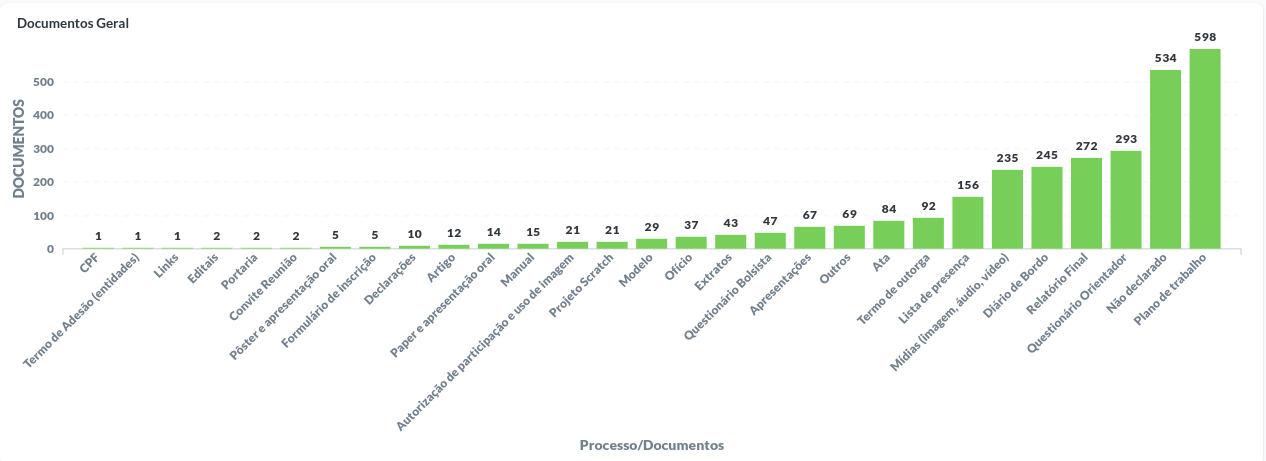
\includegraphics[max size={\textwidth}{\textheight}]{../../imagens/documentos-gerados.png}

	\end{center}

	\caption{\label{d4bddf3f657cfd53603dfd0dfc92b9c8ba526073}Distribui\c{c}\~ao de documentos no Programa WASH, segundo o estudo realizado no Recorte B, frisando que este recorte cont\'em registros de bolsistas ap\'os 2019-2020, quando o recurso foi integrado `a plataforma Platu\'oxe. (fonte:  [[WASH (2023)]]).}

\end{figure}

Os limites presentes no Recorte B quanto ao registro de documentos e bolsistas indicam que os dados da Fig. 45 s\~ao parciais, restringindo-se ao per\'{\i}odo de 2020 a 2023. Portanto, \'e razo\'avel considerar que o total de documentos no acervo do WASH \'e substancialmente maior, uma vez que o Programa se iniciou em 2013.












No que se refere \`as tem\'aticas dos planos de trabalho, utilizamos os resultados do estudo  FINK (2022), de car\'ater amostral, uma vez que \'e restrito ao per\'{\i}odo 2020 a 2021 para determinar o perfil de temas do WASH.  FINK (2022) indica uma preval\^encia da \'area \textquotedbl\{\}Ci\^encias Exatas e da Terra\textquotedbl\{\} (com 46,4\%) em rela\c{c}\~ao a \textquotedbl\{\}Ci\^encias Sociais Aplicadas\textquotedbl\{\} (com 17,8\%), \textquotedbl\{\}Ci\^encias Humanas\textquotedbl\{\} (com 17,8\%), \textquotedbl\{\}Divulga\c{c}\~ao Cient\'{\i}fica\textquotedbl\{\} (14,3\%) e \textquotedbl\{\}Ci\^encias Biol\'ogicas\textquotedbl\{\} (com 3,67\%).












Um estudo detalhado das sub\'areas de conhecimento abordadas pelos planos de trabalho do WASH \'e apresentado por FINK (2022) (ver Fig. 46). Este estudo \'e restrito ao Processo CNPq 4000172015-6, mas permite avaliar de forma amostral o perfil de temas dos projetos de pesquisa, que mostra uma distribui\c{c}\~ao com preval\^encia das tem\'aticas STEAM, ampliada da proposta original do Documento de Refer\^encia.














\captionsetup{format=plain}
\begin{figure}[htb]

	\begin{center}

		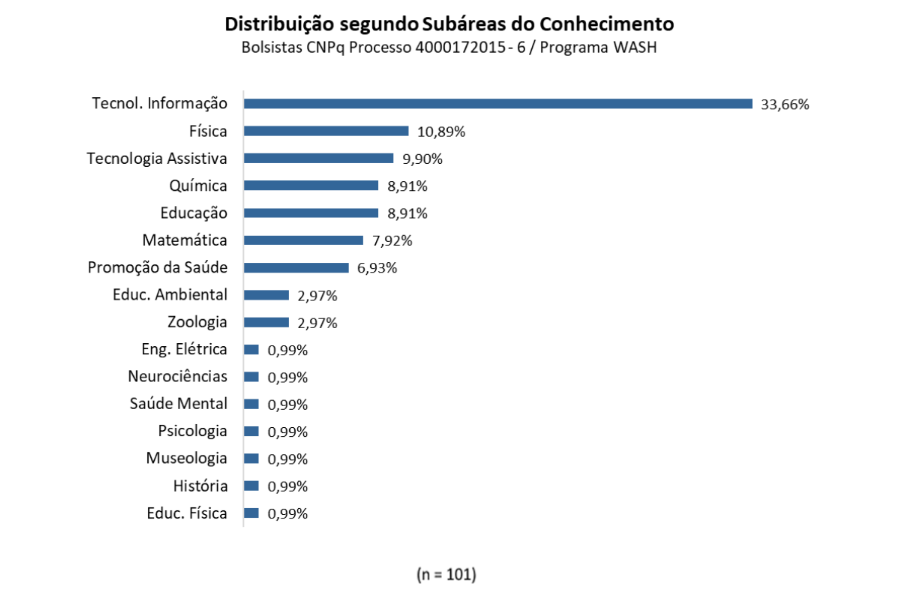
\includegraphics[max size={\textwidth}{\textheight}]{../../imagens/areas-conhecimento.png}

	\end{center}

	\caption{\label{8700d705d4d270f6322d938a607230e59db00978}Distribui\c{c}\~ao dos temas de planos de trabalho dos bolsistas de inicia\c{c}\~ao cient\'{i}fica, referentes `a emenda parlamentar associada ao Processo CNPq 4000172015-6. (fonte:  [[FINK (2022)]])}

\end{figure}

\subsection[N\'umero de eventos realizados]{N\'umero de eventos realizados}\label{N\'umero de eventos realizados}
O n\'umero de eventos realizados anualmente \'e um importante indicador da evolu\c{c}\~ao do Programa WASH, revelando, por exemplo, sua taxa de crescimento ou sua resposta a eventos externos, tais como o isolamento social imposto pela pandemia de COVID19.












Os eventos, como explicitado na se\c{c}\~ao 2.3 da Fundamenta\c{c}\~ao Te\'orica, s\~ao caracterizados pelo tipo de atividade e o tema trabalhado.












Utilizamos dados obtidos dos Recortes A e B para gerar as Figs. 47 e 48, respectivamente.












A fig. 47, referente ao Recorte A, traz a evolu\c{c}\~ao do n\'umero de eventos realizados ao longo dos 10 anos de exist\^encia do Programa, ressalvando-se que os dados para o ano de 2022 s\~ao parciais, uma vez que esse recorte se encerra em agosto de 2022.














\captionsetup{format=plain}
\begin{figure}[max size={\textwidth}{\textheight}]

\centering


\begin{minipage}[b]{0.4\linewidth}
        \centering
                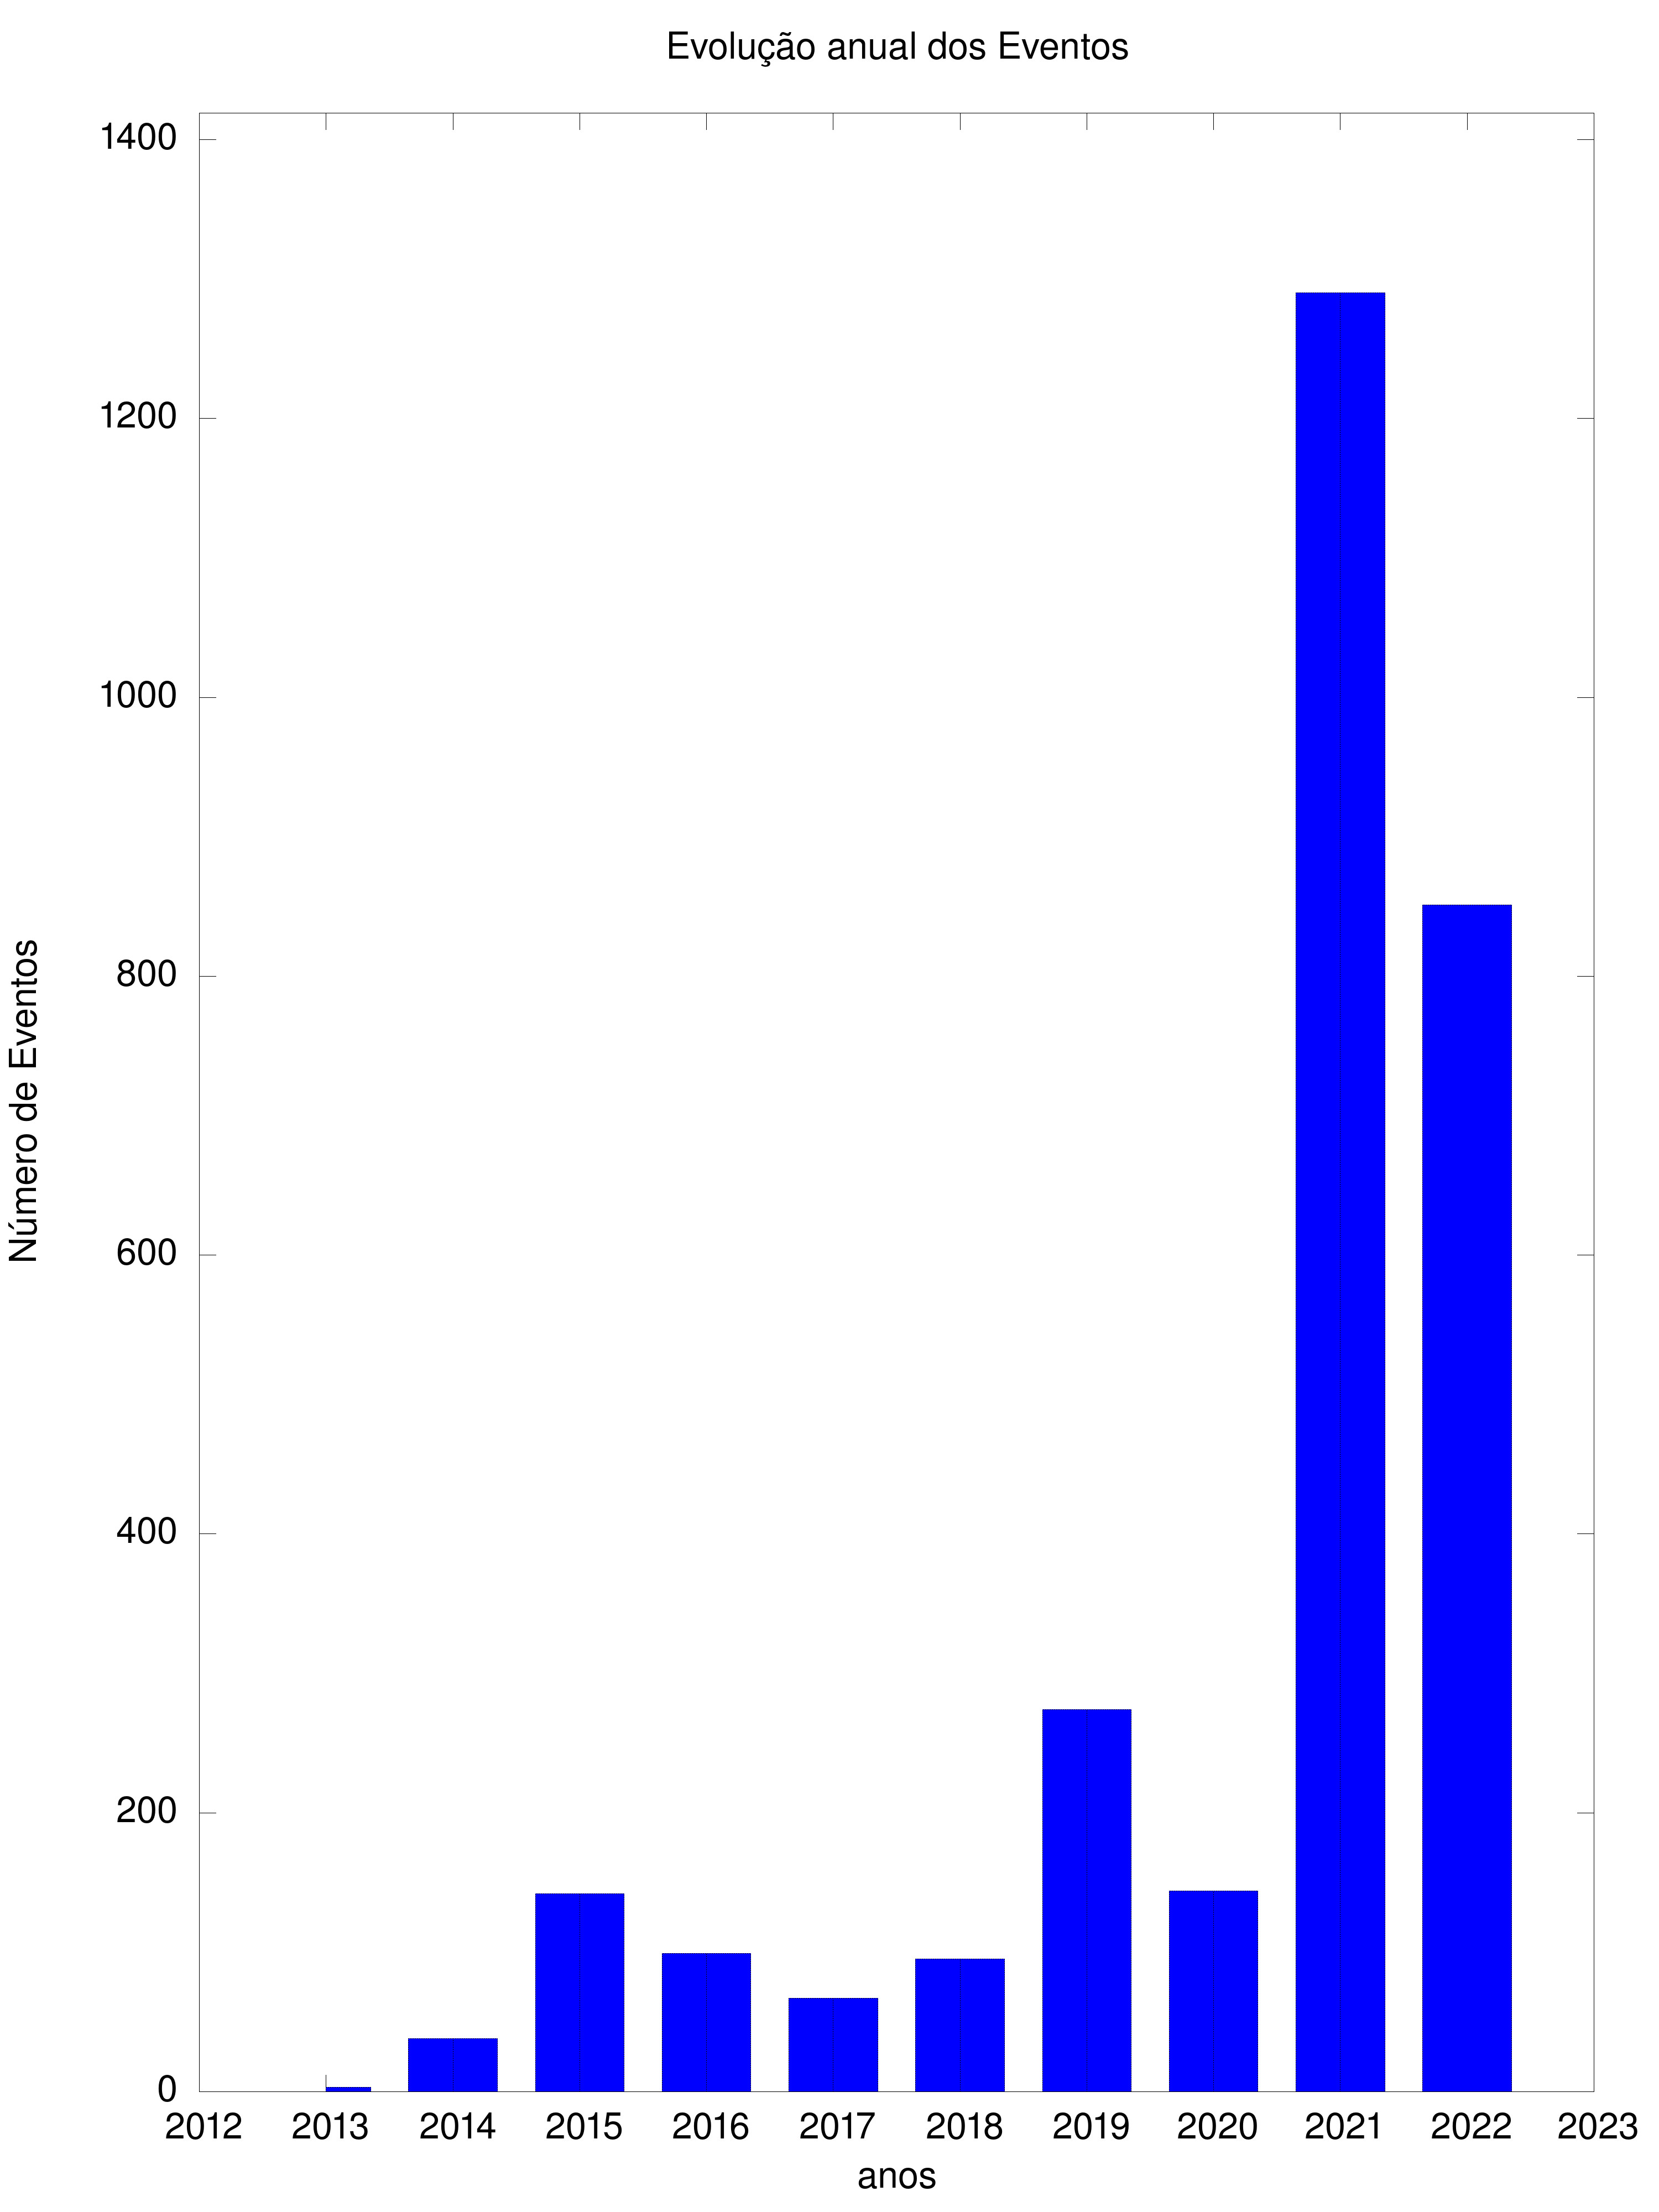
\includegraphics[width=1.0\linewidth]{../../imagens/output-eventos.jpeg}
                \caption{Evolu\c{c}\~ao anual do n\'umero de eventos realizados, obtida a partir do Recorte A. Os dados para 2022 s\~ao parciais, uma vez que a atualiza\c{c}\~ao foi interrompida em 26 de agosto de 2022.}
                \label{8af5236ba8f91623157f8f95ae10366b416d6049}
\end{minipage}%
\hspace{0.5cm}
\end{figure}



A Fig. 48 \'e referente ao Recorte B e, portanto, s\~ao os dados de janeiro de 2023 que s\~ao parciais.














\captionsetup{format=plain}
\begin{figure}[htb]

	\begin{center}

		\includegraphics[max size={\textwidth}{\textheight}]{../../imagens/eventos-ano-recorte-B.png}

	\end{center}

	\caption{\label{06b38fbf8d96a7c692475ebb4c27e84923107c5a}Evolu\c{c}\~ao anual do n\'umero de eventos com base no Recorte B. Os dados de janeiro de 2023 s\~ao parciais. (fonte:  [[WASH (2023)]])}

\end{figure}

Os gr\'aficos, independentemente do recorte escolhido, indicam um crescimento acentuado do Programa a partir de 2019, com uma interrup\c{c}\~ao em 2020, decorrente do isolamento social imposto pela pandemia. Decidimos apresentar os dois gr\'aficos para que seja poss\'{\i}vel avaliar a diferen\c{c}a entre os dados do Recorte A e B. O Recorte B \'e bem mais completo e indica a realiza\c{c}\~ao de 3.771 eventos, ao longo dos 10 anos do WASH.













\noindent\begin{center}\mbox{\centering\fbox{\centering\par\parbox{0.7\linewidth}{\small\textit{O Recorte B indica a realiza\c{c}\~ao de 3771 eventos pelo WASH.}\normalsize}}}\end{center}


O comportamento do gr\'afico de evolu\c{c}\~ao anual dos eventos \'e semelhante ao comportamento dos gr\'aficos de evolu\c{c}\~ao de participantes e participa\c{c}\~oes, j\'a mostrados na se\c{c}\~ao 4.2.4. Essa coincid\^encia refor\c{c}a a interpreta\c{c}\~ao de que o crescimento do Programa foi intensificado pela chegada de novas emendas a partir de 2019, que permitiram a expans\~ao em v\'arias localidades.












Uma an\'alise do Recorte B indicou que cerca de 22,5\% dos eventos referiram-se \`a programa\c{c}\~ao de jogos com a linguagem Scratch, segundo a declara\c{c}\~ao dos organizadores de cada evento. Esse n\'umero \'e substancialmente superior ao de qualquer outra tem\'atica abordada e pode estar subestimado, dado que depende da declara\c{c}\~ao dos organizadores.












No que se refere \`as escolas participantes, ainda dentro do Recorte B, foi poss\'{\i}vel identificar 50 escolas nominalmente nos registros. A escola E.E. Vitor Meirelles,  localizada em Campinas, se sobressaiu, representando cerca de 11\% dos registros de eventos em escolas.












Dentre as entidades promotoras, se sobressa\'{\i}ram: CTI Renato Archer (16\%), IFSP Jacare\'{\i} (17\%) e IFSP S\~ao Jos\'e dos Campos (16\%). Esse percentual de participa\c{c}\~ao \'e em rela\c{c}\~ao aos eventos com registro de entidade promotora.












\subsection[Distribui\c{c}\~ao et\'aria nos eventos]{Distribui\c{c}\~ao et\'aria nos eventos}\label{Distribui\c{c}\~ao et\'aria nos eventos}
Uma das quest\~oes fundamentais dessa pesquisa \'e verificar se o WASH realmente est\'a atingindo o p\'ublico alvo, declarado em seu documento de refer\^encia. Esse p\'ublico \'e constitu\'{\i}do de crian\c{c}as e jovens, faixas et\'arias pertinentes aos ensinos fundamental e m\'edio, respectivamente.












Uma forma de verificar essa efic\'acia de atendimento \'e organizar os dados de participa\c{c}\~ao em eventos na forma de um histograma de idades. Essa demanda, especificada pela autora, levou ao desenvolvimento de uma ferramenta de consulta estruturada espec\'{\i}fica para esse fim, a qual ficou vinculada ao Recorte A.












A Fig. 49 apresenta os histogramas de idade para os anos de 2013 a 2022. Os gr\'aficos est\~ao posicionados lado a lado em uma mesma p\'agina, com eixos cujas as escalas s\~ao id\^enticas, para que seja poss\'{\i}vel acompanhar a evolu\c{c}\~ao da forma de suas distribui\c{c}\~oes ao longo dos anos do Recorte A.












Antes de analisar a Fig. 49, \'e preciso enfatizar que os dados que originaram os histogramas s\~ao parciais, dado que os cadastros presentes na Platu\'oxe n\~ao est\~ao completos no que se refere ao ano de nascimento dos (as) participantes. Em outras palavras, os dados que geraram os histogramas s\~ao um subconjunto da amostra representada pela Platu\'oxe. A tabela participantes2, onde est\~ao registrados os cadastros, tem apenas uma fra\c{c}\~ao de registros com informa\c{c}\~ao de data de nascimento.












Mesmo com a limita\c{c}\~ao indicada, as tend\^encias observadas na Fig. 49 permitem compreender melhor a evolu\c{c}\~ao do p\'ublico alvo do WASH.














\captionsetup{format=plain}
\begin{figure}[htb]

	\begin{center}

		\includegraphics[max size={\textwidth}{\textheight}]{../../imagens/histograma-de-idades-no-ano-do-evento.png}

	\end{center}

	\caption{\label{978341992d3d49498d48c41acc77f05f08f49ead}Distribui\c{c}\~ao et\'aria dos participantes, ano a ano.}

\end{figure}

Uma observa\c{c}\~ao cuidadosa dos histogramas da Fig. 49 permitir\'a concluir que o pico das distribui\c{c}\~oes et\'arias est\'a se deslocando para a direita, com a passagem dos anos de execu\c{c}\~ao do WASH.












Esse deslocamento para a direita pode ser interpretado de duas formas:













\begin{alineas}
\item a idade m\'edia do p\'ublico alvo do WASH est\'a aumentando, com o atendimento de cada vez mais educandos jovens; e
\item a coleta de dados do WASH est\'a privilegiando o registro de participantes mais velhos, em detrimento do registro de crian\c{c}as, mascarando o real perfil et\'ario de atendimento do Programa.
\end{alineas}

\subsection[Distribui\c{c}\~ao de atividades realizadas nos eventos]{Distribui\c{c}\~ao de atividades realizadas nos eventos}\label{Distribui\c{c}\~ao de atividades realizadas nos eventos}
A distribui\c{c}\~ao de atividades realizadas durante os eventos \'e apresentada na Tabela 12. Elas podem ser classificadas como \textquotedbl\{\}atividade meio\textquotedbl\{\}, voltadas para garantir o funcionamento do WASH, e \textquotedbl\{\}fim\textquotedbl\{\}, voltadas para o atendimento do p\'ublico alvo e representam a atividade principal durante o evento, podendo haver outras atividades secund\'arias, que n\~ao est\~ao sendo consideradas.
















\begin{table}[htb]
\tiny
\caption{\label{a5eaff3e0d7afe3bcccdccd277cae286bd506174}Distribui\c{c}\~ao dos tipos de atividades realizadas durante eventos do WASH. (fonte:  [[WASH (2023)]])}

\centering
\begin{tabular}{|c|c|c|}
\hline
Atividade  &  Tipo  &  \% dos eventos \\
\hline
Apoio a Eventos  &  meio  &  0,13 \\
Apoio a Eventos de CTI  &  meio  &  0,03 \\
Apresenta\c{c}\~ao de Projetos  &  fim  &  0,60 \\
Apresenta\c{c}\~ao sobre o WASH  &  fim  &  3,04 \\
Ativ. Art\'{\i}sticas e Culturais  &  fim  &  0,17 \\
Documenta\c{c}\~ao de desenvolvimento  &  meio  &  0,77 \\
Eventos on-line  &  fim  &  0,30 \\
Oficina  &  fim  &  46,30 \\
Oficina de multiplica\c{c}\~ao  &  fim  &  1,91 \\
Palestras diversas  &  fim  &  0,17 \\
Participa\c{c}\~ao em Eventos  &  fim  &  0,20 \\
Participacao em Eventos de CTI  &  fim  &  0,37 \\
Realiza\c{c}\~ao de Eventos  &  fim  &  0,23 \\
Recep\c{c}\~ao de Visitas  &  fim  &  0,07 \\
Reuni\~ao com a Comunidade Atendida  &  fim  &  0,50 \\
Reuni\~ao com Interessados  &  fim  &  7,53 \\
Reuni\~ao da Coordenacao Geral  &  meio  &  1,37 \\
Reuni\~ao de Equipe  &  meio  &  23,55 \\
Reuni\~ao de Orienta\c{c}\~ao aos bolsistas  &  fim  &  8,03 \\
Reuni\~ao Frente Multiplicadora  &  meio  &  0,17 \\
Rodas de Conversa  &  meio  &  4,38 \\
Shows Cient\'{\i}ficos  &  fim  &  0,03 \\
Visita a entidade externa  &  fim  &  0,13 \\
\hline
  &  TOTAL MEIO  &  30,97 \\
  &  TOTAL FIM  &  69,01  \\
  &  TOTAL  &  100,00 \\
\hline
\end{tabular}
\end{table}


A Tabela mostra uma preval\^encia das atividades fim (69\%) em rela\c{c}\~ao \`as atividades meio (31\%).












\subsection[Cidades Atendidas]{Cidades Atendidas}\label{Cidades Atendidas}
Com base no Recorte B foi poss\'{\i}vel levantar a lista de cidades alcan\c{c}adas pelo WASH, em v\'arios contextos. Este levantamento foi feito por meio de consultas estruturadas, aplicadas \`a Platu\'oxe. Cabe relembrar que os dados dessa plataforma s\~ao uma amostra do total de atividades efetivamente realizadas pelo WASH.












Na Fig. 50, vemos o gr\'afico da distribui\c{c}\~ao dos bolsistas em fun\c{c}\~ao das cidades brasileiras onde est\~ao radicados. Por meio de legendas coloridas, o gr\'afico permite visualizar, simultaneamente, as distribui\c{c}\~oes de modalidades de bolsas por essas cidades. Note que n\~ao se tratam de cidades onde, necessariamente, ocorreram eventos do WASH. As cidades est\~ao ordenadas em ordem alfab\'etica.














\captionsetup{format=plain}
\begin{figure}[htb]

	\begin{center}

		\includegraphics[max size={\textwidth}{\textheight}]{../../imagens/distribuicao-bolsistas-por-cidades.png}

	\end{center}

	\caption{\label{272b812569e747beabce0484704c884a06f72e19}Distribui\c{c}\~ao das localidades onde bolsistas do WASH est\~ao radicados. (fonte:  [[WASH (2023)]])}

\end{figure}

A Fig. 51 traz a distribui\c{c}\~ao de eventos do WASH por cidades brasileiras.














\captionsetup{format=plain}
\begin{figure}[htb]

	\begin{center}

		\includegraphics[max size={\textwidth}{\textheight}]{../../imagens/eventos-cidades.png}

	\end{center}

	\caption{\label{f08c4c52c76dddcb99c8ad9685858f3c5990432d}Distribui\c{c}\~ao de eventos do WASH pelas cidades brasileiras. (fonte:  [[WASH (2023)]])}

\end{figure}

\subsection[Canal do WASH e a webs\'erie \textquotedbl\{\}Ci\^encia e Cultura Vamos Brincar?\textquotedbl\{\}]{Canal do WASH e a webs\'erie \textquotedbl\{\}Ci\^encia e Cultura Vamos Brincar?\textquotedbl\{\}}\label{Canal do WASH e a webs\'erie \textquotedbl\{\}Ci\^encia e Cultura Vamos Brincar?\textquotedbl\{\}}
O WASH disp\~oe de um canal na rede social Youtube para a dissemina\c{c}\~ao de sua produ\c{c}\~ao audiovisual, que \'e uma parte importante do resultado do trabalho dos alunos dos ensinos fundamental e m\'edio. Este canal \'e designado \textquotedbl\{\} Programa WASH \textquotedbl\{\} e seu acervo est\'a aberto para acesso ilimitado.












S\~ao 427 v\'{\i}deos carregados no canal desde 14 de dezembro de 2019, quando o canal foi criado. Anteriormente a essa data, os v\'{\i}deos do WASH eram \textquotedbl\{\}carregados\textquotedbl\{\} nos canais individuais de membros da equipe.












Segundo o sistema de estat\'{\i}stica do pr\'oprio Youtube, o canal teve 56.816 visualiza\c{c}\~oes at\'e fevereiro de 2023, divididas entre os 427 v\'{\i}deos. A produ\c{c}\~ao \'e muito variada, contendo anima\c{c}\~oes, dicas sobre programa\c{c}\~ao, \textquotedbl\{\}stop motion\textquotedbl\{\}, oficinas, entrevistas, conta\c{c}\~ao de est\'orias, v\'{\i}deos tipo \textquotedbl\{\}fa\c{c}a voc\^e mesmo\textquotedbl\{\}, m\'usicas, etc.












Consta do acervo do canal \textquotedbl\{\}Programa WASH\textquotedbl\{\}, a edi\c{c}\~ao de nove epis\'odios da webs\'erie \textquotedbl\{\}Ci\^encia e Cultura, vamos brincar?\textquotedbl\{\} (CCVB). Esse programa, como j\'a explicado na se\c{c}\~ao 4.1.6, foi criado como forma alternativa de promover a aprendizagem no contexto da pandemia, quando as oficinas presenciais n\~ao eram mais poss\'{\i}veis. O CCVB foi concebido por esta autora, que coordenou suas atividades.












A produ\c{c}\~ao do CCVB contou com a participa\c{c}\~ao de dezenas de colaboradores, divididos em tr\^es grupos principais  (WASHCNPq, 2022):













\begin{alineas}
\item WASH: esfor\c{c}o coordenado pela autora;
\item \textquotedbl\{\}N\'os somos a Ci\^encia\textquotedbl\{\}: iniciativa livre, coordenada pelo divulgador cient\'{\i}fico Will Namen, que posteriormente se integrou \`a equipe do WASH; e
\item Cia. Bola de Meia: esfor\c{c}o coordenado por Jacqueline Baumgratz e Celso Pan, que posteriormente passaram  a integrar tamb\'em a equipe do WASH.
\end{alineas}

Foram nove epis\'odios publicados no Youtube, listados a seguir.













\begin{alineas}
\item Epis\'odio 1: Lan\c{c}amento
\item Epis\'odio 2: Astronomia, ci\^encia e arte
\item Epis\'odio 3: \'Agua, vida, direito, dever e poder
\item Epis\'odio 4: Fauna, flora e fogo
\item Epis\'odio 5: A crian\c{c}a e a ci\^encia
\item Epis\'odio 6: Sistema Solar
\item Epis\'odio 7: Vacina
\item Epis\'odio 8: Mudan\c{c}as Clim\'aticas
\item Epis\'odio 9: Acessibilidade
\end{alineas}

Posteriormente \`a estr\'eia no Youtube, mediante solicita\c{c}\~ao formal, esses epis\'odios foram disponibilizados para TVs Abertas e \textquotedbl\{\}a cabo\textquotedbl\{\}, tendo sido veiculados por VRT, TV Taubat\'e e TVT.












\section[Linhas de Tempo]{Linhas de Tempo}\label{Linhas de Tempo}
Neste ponto do texto \'e poss\'{\i}vel consolidar na forma de \textquotedbl\{\}linhas do tempo\textquotedbl\{\} os conhecimentos obtidos a partir do emprego dos m\'etodos relacionados aos eixos 1 e 2.












Constru\'{\i}mos 3 linhas que s\~ao apresentadas nas se\c{c}\~oes a seguir.












\subsection[Trajet\'oria do Programa WASH]{Trajet\'oria do Programa WASH}\label{Trajet\'oria do Programa WASH}
O mapa da Fig. 52 apresenta, por dec\^enio, os principais fatos que contribu\'{\i}ram para o Programa WASH, com marcos hist\'oricos nacionais e internacionais, incluindo o papel desempenhado por pessoas, bem como os contextos que marcaram a trajet\'oria do Programa WASH.














\captionsetup{format=plain}
\begin{figure}[htb]

	\begin{center}

		\includegraphics[max size={\textwidth}{\textheight}]{../../imagens/Linha-do-Tempo-trajetoria-WASH-1.png}

	\end{center}

	\caption{\label{e12291971a1551c08a11d25104283d4772778aaf}Linha do tempo representando a trajet\'oria do WASH (produ\c{c}\~ao pr\'opria)}

\end{figure}

\'E poss\'{\i}vel identificar ra\'{\i}zes do Programa WASH nas d\'ecadas de 60 e 70 do s\'eculo passado, quando uma comunidade em torno de uma dita \textquotedbl\{\}cultura digital\textquotedbl\{\} come\c{c}ou a se formar. Nessas d\'ecadas \'e poss\'{\i}vel encontrar o pioneirismo de Jos\'e Ellis Ripper Filho, Alfred Volkmer e Andr\'as G. V\'as\'arhelyl, criadores do primeiro computador digital brasileiro no Instituto Tecnol\'ogico da Aeron\'autica. Essa iniciativa pioneira em S\~ao Jos\'e dos Campos foi seguida pela cria\c{c}\~ao do \textquotedbl\{\}Patinho Feio\textquotedbl\{\}, marco do desenvolvimento da Computa\c{c}\~ao na Universidade de S\~ao Paulo. Foi na d\'ecada de 60 que a Profa. Dra. Afira Ripper se transferiu para os Estados Unidos, estabelecendo o primeiro contato com a equipe de Papert, no MIT.












A cria\c{c}\~ao dos laborat\'orios de microeletr\^onica, tanto na USP como na Unicamp, tamb\'em s\~ao elementos de import\^ancia para entender a concep\c{c}\`ao do WASH, uma vez que desses laborat\'orios decorreu a cria\c{c}\~ao do Centro de Tecnologia para a Inform\'atica, em 1982, sucedido pelo Centro de Tecnologia da Informa\c{c}\~ao Renato Archer, ber\c{c}o do WASH.












Outro ponto inclu\'{\i}do na linha do tempo foi o estudo pioneiro no Brasil, realizado pela Profa. Cec\'{\i}lia Baranauskas, em torno da avalia\c{c}\~ao da aplica\c{c}\~ao da linguagem LOGO para crian\c{c}as












No intuito de mostrar as interrela\c{c}\~oes entre atores envolvidos com a cria\c{c}\~ao dessa \textquotedbl\{\}cultura digital\textquotedbl\{\}, inclu\'{\i}mos na linha do tempo a participa\c{c}\~ao do Prof. Jos\'e Ellis Ripper Filho no conselho do Centre Mondiale, quando esse centro de pesquisa franc\^es era dirigido por Nicholas Negroponte.












Finalmente, inclu\'{\i}mos alguns fatos relacionados com a atua\c{c}\~ao da autora, a exemplo da contribui\c{c}\~ao para a cria\c{c}\~ao de um sistema pioneiro de gest\~ao para sa\'ude (SOL), ou a participa\c{c}\~ao no Planejamento Estrat\'egico da Casa Civil para ado\c{c}\~ao do Software Livre pelo Governo Federal, dentre tantos outros.












\subsection[Trajet\'oria de Pol\'{\i}ticas P\'ublicas]{Trajet\'oria de Pol\'{\i}ticas P\'ublicas}\label{Trajet\'oria de Pol\'{\i}ticas P\'ublicas}
Neste ponto apresentamos uma linha do tempo das pol\'{\i}ticas p\'ublicas que, na nossa concep\c{c}\~ao, s\~ao pertinentes ao programa WASH (ver Fig. 53).














\captionsetup{format=plain}
\begin{figure}[htb]

	\begin{center}

		\includegraphics[max size={\textwidth}{\textheight}]{../../imagens/ Linha-do-Tempo-Politicas-Digitais Publicas-egov-2.png}

	\end{center}

	\caption{\label{435840ce031a949680fc4fef81afb2709efc0253}Linha do tempo representando a evolu\c{c}\~ao das pol\'{i}ticas p\'ublicas para o setor digital no Brasil (produ\c{c}\~ao pr\'opria)}

\end{figure}

A cria\c{c}\~ao do CNPq na d\'ecada de 50 \'e o grande marco para toda a \'area de ci\^encia e tecnologia brasileira. N\~ao poderia ser diferente para o WASH, que depende da estrutura do CNPq para garantir a concess\~ao de suas bolsas e avalia\c{c}\~ao de seus resultados. Por raz\~oes de escala, n\~ao foi poss\'{\i}vel representar na Fig. 53 o momento de cria\c{c}\~ao do CNPq. O primeiro fato registrado na figura \'e a cria\c{c}\~ao do Minist\'erio da Ci\^encia e Tecnologia, posterior, inclusive, \`a cria\c{c}\~ao do CTI Renato Archer.












O programa de inicia\c{c}\~ao cient\'{\i}fica para o ensino superior do CNPq foi criado em 1988 e posteriormente foi ampliado para o ensino m\'edio. A linha do tempo mostra tamb\'em o momento em que se iniciaram as discuss\~oes sobre governo eletr\^onico, seguido da cria\c{c}\~ao do GESAC, entre outros programas voltados para o setor digital.












\subsection[Consolida\c{c}\~ao das linhas de tempo]{Consolida\c{c}\~ao das linhas de tempo}\label{Consolida\c{c}\~ao das linhas de tempo}
O mapa da Fig. 54 consolida a hist\'oria do Programa WASH, atrav\'es da jun\c{c}\~ao da linha do tempo “Trajet\'oria Programa WASH” com o mapa “Pol\'{\i}ticas Digitais P\'ublicas”, e integrando dados sobre o desenvolvimento da linguagem SCRATCH.














\captionsetup{format=plain}
\begin{figure}[htb]

	\begin{center}

		\includegraphics[max size={\textwidth}{\textheight}]{../../imagens/Linha-do-Tempo-WASH-GERAL-4.png}

	\end{center}

	\caption{\label{7f3511906917a26c6f99731c141fb046fe43495d}Consolida\c{c}\~ao das linhas do tempo do Projeto WASH (produ\c{c}\~ao pr\'opria)}

\end{figure}

\section[Valida\c{c}\~ao das hip\'oteses]{Valida\c{c}\~ao das hip\'oteses}\label{Valida\c{c}\~ao das hip\'oteses}
A partir da s\'{\i}ntese dos resultados  dos eixos 1 e 2 ser\'a realizada  a valida\c{c}\~ao das hip\'oteses levantadas na introdu\c{c}\~ao.












\subsection[Hip\'otese 1: Efici\^encia e Efic\'acia do WASH]{Hip\'otese 1: Efici\^encia e Efic\'acia do WASH}\label{Hip\'otese 1: Efici\^encia e Efic\'acia do WASH}
Come\c{c}aremos a valida\c{c}\~ao da Hip\'otese 1 por meio da abordagem da efic\'acia, utilizando os resultados do eixo 2, como base para a an\'alise.












Empregaremos como medi\c{c}\~ao de efic\'acia a capacidade do WASH de atender o p\'ublico alvo definido em seu Documento de Refer\^encia.












O paralelo entre \textquotedbl\{\} p\'ublico alvo \textquotedbl\{\} e efic\'acia busca retirar da an\'alise, neste momento, os indicadores relacionados \`a efici\^encia, que ser\~ao tratados a seguir (e.g. n\'umero de benefici\'arios do Programa). Nesse racioc\'{\i}nio, consideramos o WASH eficaz caso o p\'ublico alvo atendido seja aquele especificado no Documento de Refer\^encia, comparando a quantidade relativa de crian\c{c}as (fundamental), jovens (m\'edio e superior) e adultos, independentemente de quantidade absoluta do somat\'orio desses tr\^es grupos.












Considerando a linguagem de Peter Drucker (ver Fundamenta\c{c}\~ao Te\'orica) sobre efic\'acia, trazida na se\c{c}\~ao 2.2.1, atingir o p\'ublico alvo \'e \textquotedbl\{\}fazer a coisa certa\textquotedbl\{\}, ou seja, cumprir com um objetivo expl\'{\i}cito do Programa.












No Documento de Refer\^encia  (CTI, 2018), que estabelece \textquotedbl\{\}o que o WASH gostaria de ter sido\textquotedbl\{\}, identificamos que deveria haver, no que tange ao p\'ublico alvo do WASH, uma preponder\^ancia dos alunos do ensino fundamental (ver se\c{c}\~ao 4.2.6) em rela\c{c}\~ao aos alunos do ensino m\'edio e superior.












Pelo lado dos resultados alcan\c{c}ados via eixo 2, que indicam \textquotedbl\{\}o que o WASH conseguiu ser\textquotedbl\{\}, revelamos em que medida o p\'ublico alvo, explicitado pelo  Documento de Refer\^encia foi alcan\c{c}ado. Ou seja, apresentamos indica\c{c}\~oes da efic\'acia do WASH. Fazemos isso expondo dois indicadores do Programa com vistas a avaliar sua efic\'acia, a saber:













\begin{alineas}
\item os histogramas de idades da Fig. 49, oriundos do Recorte A da Platu\'oxe, indicam picos de participantes na faixa de 10 a 16 anos, entre  2013 e 2019. N\~ao obstante o car\'ater amostral do Recorte A, porque n\~ao traz a totalidade de cadastros, o fato \'e que tal faixa et\'aria \'e compat\'{\i}vel com um p\'ublico alvo representativo do ensino fundamental. No entanto, para os anos de 2020 a 2022, identificamos um deslocamento \`a direita da posi\c{c}\~ao do pico, que chega a 19 anos, em 2022. Essa situa\c{c}\~ao poderia ser um indicativo de perda de efic\'acia do Programa, dado que seria um sinal de desvio de seu p\'ublico alvo (i.e. faixa et\'aria acima da almejada). Mas, segundo o que j\'a discutimos na se\c{c}\~ao 4.2.3, essa tend\^encia de crescimento da idade dos participantes verificada no Recorte A pode estar associada \`a coleta de dados deficiente, uma vez que a alimenta\c{c}\~ao de dados sobre crian\c{c}as participantes foi sendo reduzida pelos parceiros. Essa defici\^encia de coleta de dados foi associada ao advento da LGPD, dentre outros fatores.  Parece-nos que essa situa\c{c}\~ao \textquotedbl\{\}distorcida\textquotedbl\{\}  da amostra, a partir de 2020, \'e  mais prov\'avel do que um aumento da idade m\'edia dos participantes, exceto para o ano de 2020, quando a pandemia pode ter influenciado, tamb\'em, o perfil do p\'ublico alvo.
\item a distribui\c{c}\~ao dos tipos de modalidades de bolsas, mostrada na Fig. 43, obtida do Recorte B da Platu\'oxe, embora de car\'ater tamb\'em amostral, indica uma preval\^encia de bolsistas de inicia\c{c}\~ao cient\'{\i}fica (cerca de 75\%), que t\^em o papel de ser  multiplicador das oficinas WASH para o ensino fundamental.
\end{alineas}

As duas considera\c{c}\~oes acima indicam que o WASH tem sido bem-sucedido em focalizar o ensino fundamental como p\'ublico alvo, o que torna poss\'{\i}vel validar a primeira parte da Hip\'otese 1, i.e. efic\'acia. As evid\^encias de perda de representatividade das amostras, a partir de 2020, sugerem-nos descartar um poss\'{\i}vel desvio do p\'ublico alvo do Programa, a menos de um plaus\'{\i}vel desvio do p\'ublico alvo restrito a 2020, decorrente da fase inicial do isolamento social da pandemia. Esse comportamento discrepante \'e compat\'{\i}vel com a queda no n\'umero de eventos naquele ano, presente tanto na Fig. 47 quanto na Fig. 48.












Na linguagem de Peter Drucker, a efici\^encia se refere a \textquotedbl\{\}fazer do jeito certo\textquotedbl\{\}, abrindo a porta para tra\c{c}ar um paralelo com a quantidade de eventos realizados, a quantidade de benefici\'arios e a rela\c{c}\~ao atividade fim/meio. Esse racioc\'{\i}nio reflete a ideia de que se os processos do WASH forem eficientes (i.e. \textquotedbl\{\}feitos da forma correta\textquotedbl\{\}), mais pessoas ser\~ao atendidas com o mesmo recurso financeiro, independentemente dessas pessoas serem parte do p\'ublico alvo (i.e. ensino fundamental).












O primeiro aspecto para medir a efici\^encia \'e considerar o n\'umero de cadastros de participantes, oriundo do Recorte A da Platu\'oxe, que aponta 3.265 pessoas. Mostramos, pela identifica\c{c}\~ao de eventos em que os participantes n\~ao foram contabilizados (se\c{c}\~ao 4.2.3), que este n\'umero est\'a subavaliado. O n\'umero efetivo de participantes \'e pass\'{\i}vel de ser substancialmente maior, n\~ao havendo uma forma confi\'avel de apresentar um n\'umero consolidado. Por exemplo, o uso das imagens dos eventos para tentar corrigir o n\'umero efetivamente registrado na plataforma seria um m\'etodo muito impreciso, dado que as imagens s\~ao parciais.












Seja como for, se consider\'assemos a quantidade de 3.265 participantes, isoladamente, chegar\'{\i}amos a uma avalia\c{c}\~ao de que o WASH \'e ineficiente no atendimento de pessoas, dado que \'e um n\'umero relativamente pequeno. Por outro lado, essa avalia\c{c}\~ao n\~ao seria justa, dado que sabemos que esse n\'umero \'e subvalorado. O n\'umero de visualiza\c{c}\~oes do canal do WASH no Youtube, combinado com o alcance da divulga\c{c}\~ao do Programa nas TVs abertas e a cabo, tenderia a pender a balan\c{c}a da avalia\c{c}\~ao para o campo da efici\^encia, dado que s\~ao n\'umeros bastante expressivos.












Mas, o atendimento preponderante de alunos do fundamental n\~ao \'e o \'unico objetivo expresso no Documento de Refer\^encia do WASH. A realiza\c{c}\~ao de inicia\c{c}\~ao cient\'{\i}fica \'e um outro aspecto importante. Nesse quesito, o n\'umero de bolsistas \'e outro indicador importante de efic\'acia, com centenas de participantes, os quais produziram centenas de planos de trabalho, relat\'orios e audiovisuais, bem como centenas de joguinhos de computador registrados na plataforma do Scratch, do MIT. Entendemos que essa quantidade de produ\c{c}\~ao corrobora com uma avalia\c{c}\~ao de efici\^encia do Programa. No campo da efic\'acia, o perfil de bolsistas, concentrado em torno de alunos do ensino m\'edio (ver se\c{c}\~ao 4.2.6), indica que o Programa atendeu suas diretrizes originas.












Outro aspecto que pode ser usado para a avalia\c{c}\~ao da efici\^encia do Programa \'e o balan\c{c}o de atividades, classificadas nos tipos \textquotedbl\{\}meio\textquotedbl\{\} e \textquotedbl\{\}fim\textquotedbl\{\}. Como vimos na se\c{c}\~ao 4.2.10, h\'a uma quantidade relativamente grande de atividades fim (cerca de 69\%).












Com tudo isso em considera\c{c}\~ao, acreditamos ser poss\'{\i}vel validar a Hip\'otese 1, tanto no campo da efic\'acia (p\'ublico alvo) quanto no campo da efici\^encia (milhares de benefici\'arios), com ressalvas para a qualidade da coleta de dados, que ainda n\~ao permitiu obter um n\'umero consolidado de participantes e participa\c{c}\~oes, dado o car\'ater amostral dessa coleta. Tamb\'em o n\'umero de visualiza\c{c}\~oes do canal do WASH no ,Youtube, \'e um tanto question\'avel, porque os crit\'erio de contabiliza\c{c}\~ao daquela rede social n\~ao \'e claros. Os dados de espectadores dos canais abertos e de TV a cabo n\~ao foram levantados, n\~ao havendo uma estimativa validada no momento.












\subsection[Hip\'otese 2: Orienta\c{c}\~ao a Projetos]{Hip\'otese 2: Orienta\c{c}\~ao a Projetos}\label{Hip\'otese 2: Orienta\c{c}\~ao a Projetos}
No que se refere ao emprego de um m\'etodo de aprendizagem por \textquotedbl\{\}orienta\c{c}\~ao a projeto\textquotedbl\{\}, sentimo-nos confiantes em validar a presente hip\'otese. Essa valida\c{c}\~ao \'e poss\'{\i}vel por conta da expressiva quantidade de bolsas concedidas, resultantes em centenas de relat\'orios de projeto, publica\c{c}\~oes cient\'{\i}ficas, audiovisuais, dentre tantas outras produ\c{c}\~oes ocorridas no contexto dos projetos de cada bolsista. As tem\'aticas de projetos levantadas, em car\'ater amostral (ver se\c{c}\~ao 4.2.7), confirmam que os projetos se deram no contexto do STEM, como previsto no Documento de Refer\^encia.












\subsection[Hip\'otese 3: Origem do WASH]{Hip\'otese 3: Origem do WASH}\label{Hip\'otese 3: Origem do WASH}
O levantamento historiogr\'afico permite sustentar a validade desta hip\'otese, porque confirmou a exist\^encia de elementos que ligam a origem do WASH a Orogramas pregressos, tais como o GESAC, O OLPC e o PID, inclusive com superposi\c{c}\~ao de atores, m\'etodos de trabalho, objetivos e formas de organiza\c{c}\~ao. Tamb\'em foi poss\'{\i}vel identificar o trabalho da Profa. Afira Ripper como um dos elementos de inspira\c{c}\~ao dos m\'etodos do WASH.












\subsection[Hip\'otese 4: Pr\'atica Pedag\'ogica do WASH]{Hip\'otese 4: Pr\'atica Pedag\'ogica do WASH}\label{Hip\'otese 4: Pr\'atica Pedag\'ogica do WASH}
A \^enfase em pr\'aticas oriundas da pedagogia de Papert est\'a evidente no Programa WASH, principalmente pela preval\^encia de oficinas voltadas para o uso de programa\c{c}\~ao de computadores (linguagem Scratch).












Muito embora tenha travado contato com o pensamento de Papert, por meio da avalia\c{c}\~ao do Projeto OLPC (ver se\c{c}\~ao 4.1.2), um projeto de educa\c{c}\~ao baseado na aquisi\c{c}\~ao de notebooks, o WASH optou por um caminho diferente. Optou por concentrar todo o seu investimento em pessoas, sem propor a compra de equipamentos. Na concep\c{c}\~ao do WASH, o investimento em pessoas \'e feito por meio de bolsas do CNPq, aproveitando a infraestrutura e equipamentos j\'a existentes nas escolas e demais entidades respons\'aveis participantes para otimizar o uso de recursos.  Mesmo com essa diferen\c{c}a em rela\c{c}\~ao ao OLPC, acreditamos que seja poss\'{\i}vel validar integralmente esta hip\'otese.












\subsection[Hip\'otese 5: WASH como proto-pol\'{\i}tica p\'ublica]{Hip\'otese 5: WASH como proto-pol\'{\i}tica p\'ublica}\label{Hip\'otese 5: WASH como proto-pol\'{\i}tica p\'ublica}
O WASH se iniciou como uma atividade volunt\'aria de oferta de oficinas de tecnologia para crian\c{c}as e jovens de baixa renda, aos finais de semana,  sem financiamento. O fato do Programa, mesmo em car\'ater volunt\'ario, ter sido concebido e executado no seio de uma institui\c{c}\~ao de pesquisas federal (CTI Renato Archer), abriu uma oportunidade para propor sua evolu\c{c}\~ao para a condi\c{c}\~ao de projeto institucional. O sucesso das atividades foi demandando a repeti\c{c}\~ao dos projetos, ano ap\'os ano. A grande quantidade de projetos deu-lhe as caracter\'{\i}sticas de um programa, embora nunca tenha sido formalizado como tal na esfera federal.  Hoje, pode ser considerado como uma protopol\'{\i}tica p\'ublica nacional. Para sustentar essa hip\'otese, podemos considerar a variedade de documentos formais de ades\~ao ao seu m\'etodo, emitidos por autoridades p\'ublicas, bem como a grande quantidade de emendas parlamentares concedidas. Assim, o WASH n\~ao fica restrito ao v\'{\i}nculo com a administra\c{c}\~ao p\'ublica federal, estabelecendo pontes com os demais entes federados, com os poderes executivo e legislativo, com as redes de ensino, com os \'org\~aos de fomento cient\'{\i}fico e com as organiza\c{c}\~oes sociais.












Para que o WASH transite da condi\c{c}\~ao de protopol\'{\i}tica p\'ublica, h\'a que se institucionaliz\'a-lo por meio de instrumento jur\'{\i}dico e estruturas  adequados para a cria\c{c}\~ao efetiva de Programas, no \^ambito federal.












\subsection[Hip\'otese 6: WASH como organiza\c{c}\~ao heter\'arquica]{Hip\'otese 6: WASH como organiza\c{c}\~ao heter\'arquica}\label{Hip\'otese 6: WASH como organiza\c{c}\~ao heter\'arquica}
Vimos que o WASH n\~ao est\'a cristalizado, por meio de instrumento jur\'{\i}dico, no seio de uma institui\c{c}\~ao federal. A Portaria CTI 178/2018 traz um conjunto de conceitos, uma descri\c{c}\~ao do m\'etodo de execu\c{c}\~ao do WASH e da sua organiza\c{c}\~ao, sem o poder de vincular qualquer ator da administra\c{c}\~ao p\'ublica a esses des\'{\i}gnios.












A ades\~ao ao WASH se d\'a pela express\~ao da vontade unilateral de gestores p\'ublicos e de parceiros que, ao publicarem termos de ades\~ao ao Documento de Refer\^encia, assumem um compromisso com a sociedade de que aqueles des\'{\i}gnios ser\~ao seguidos.












Portanto, n\~ao existe rela\c{c}\~ao hier\'arquica entre as entidades aderentes ao \textquotedbl\{\}Programa\textquotedbl\{\}.












Similarmente, o WASH n\~ao tem organograma, sendo desenvolvido exclusivamente por bolsistas, cujas obriga\c{c}\~oes profissionais est\~ao definidas num termo de outorga, expedido pelo CNPq no momento de concess\~ao da bolsa. Portanto, n\~ao existe rela\c{c}\~ao hier\'arquica entre os profissionais, que se organizam para dividir tarefas de forma colegiada, em estruturas que no WASH foram denominadas \textquotedbl\{\}frentes\textquotedbl\{\}, a exemplo da citada \textquotedbl\{\}Frente Multiplicadora\textquotedbl\{\} (ver se\c{c}\~ao 4.2.6).












Portanto, \`a luz do que foi discutido na Fundamenta\c{c}\~ao Te\'orica sobre as diferen\c{c}as entre hierarquia e heterarquia, avaliamos que \'e poss\'{\i}vel validar a presente hip\'otese, confirmando que o WASH se organiza na forma de heterarquia.












\chapter[CONCLUS\~OES]{CONCLUS\~OES}\label{CONCLUS\~OES}
O primeiro aspecto que buscamos mostrar nesta disserta\c{c}\~ao \'e que o WASH nasceu no bojo de uma tradi\c{c}\~ao particular de programas de educa\c{c}\~ao, alfabetiza\c{c}\~ao cient\'{\i}fica e tecnol\'ogica, cultura digital e inclus\~ao social/digital.












Como caracter\'{\i}stica geral, essa tradi\c{c}\~ao tem por pano de fundo a busca pela inser\c{c}\~ao do indiv\'{\i}duo em sua pr\'opria cultura, atrav\'es da promo\c{c}\~ao de viv\^encias n\~ao padronizadas e n\~ao impostas por uma estrutura central.












Em outras palavras, identifica-se nessas tradi\c{c}\~oes a promo\c{c}\~ao de eventos de intera\c{c}\~ao humana, com \^enfase num ideal de justi\c{c}a social, distribu\'{\i}dos temporalmente e geograficamente, concebidos para garantir que essas intera\c{c}\~oes se deem no contexto da aprendizagem.












Pensando na met\'afora do \textquotedbl\{\}segundo dil\'uvio\textquotedbl\{\} de Ascott, citado na Introdu\c{c}\~ao, \'e inevit\'avel tra\c{c}ar um paralelo entre os programas GESAC, PID e OLPC como a \textquotedbl\{\}Arca de No\'e\textquotedbl\{\}, que permitiu sobreviv\^encia a esse \textquotedbl\{\}dil\'uvio\textquotedbl\{\}.












Ali\'as, na Introdu\c{c}\~ao, antecip\'aramos uma das conclus\~oes desta disserta\c{c}\~ao que aqui depois de todo o trabalho,  sentimos-nos mais confiantes em vaticinar:













\noindent\begin{center}\mbox{\centering\fbox{\centering\par\parbox{0.7\linewidth}{\small\textit{A exist\^encia do WASH pode  ser compreendida como mais um esfor\c{c}o - mais uma \textquotedbl\{\}Arca de No\'e\textquotedbl\{\} dos novos tempos, que ajuda na sobreviv\^encia e nos prepara para o \textquotedbl\{\}dil\'uvio informacional\textquotedbl\{\}, identificado por Ascott.}\normalsize}}}\end{center}


Assim,  o WASH compartilha caracter\'{\i}sticas em comum com os programas GESAC, PID e OLPC, estudados neste trabalho. Dentre estas caracter\'{\i}sticas podemos enunciar:













\begin{alineas}
\item o foco na aprendizagem e n\~ao no ensino;
\item o car\'ater estritamente p\'ublico e n\~ao vinculado a interesses comerciais;
\item a ado\c{c}\~ao do lema: \textquotedbl\{\}ensinar como pretexto para aprender\textquotedbl\{\};
\item o est\'{\i}mulo \`a produ\c{c}\~ao de conte\'udos pelos pr\'oprios educandos, respeitando seu protagonismo, em detrimento de um \textquotedbl\{\}conteudismo impositivo\textquotedbl\{\};
\item o respeito pelas caracter\'{\i}sticas e realidades locais, sem imposi\c{c}\~oes sobre a forma de atua\c{c}\~ao;
\item o respeito \`as lideran\c{c}as, aos coordenadores que se consolidam na organiza\c{c}\~ao e gest\~ao dos trabalhos;
\item a falta de controle centralizado vertical, em que uma ordem consensual impera, estabelecendo-se uma organiza\c{c}\~ao heter\'arquica;
\item a promo\c{c}\~ao e o uso das tecnologias livres;
\item o m\'etodo cient\'{\i}fico como valor fundamental.
\end{alineas}

A no\c{c}\~ao de que o WASH \'e um ep\'{\i}tome de uma forma de pensar as pol\'{\i}ticas p\'ublicas, se comprova pelo estudo que fizemos de suas origens.












A aplica\c{c}\~ao do nosso m\'etodo historiogr\'afico mostrou que o WASH \textquotedbl\{\}bebeu na fonte\textquotedbl\{\} das iniciativas pregressas citadas, transformando-as para suplantar suas defici\^encias.  Por exemplo, diferentemente do GESAC, PID e OLPC, o WASH optou por direcionar todos os seus recursos para o investimento em pessoas, por meio de suas atividades, e na forma de bolsas de diferentes modalidades, em detrimento do investimento em equipamentos. Al\'em disso, na busca de mais inclus\~ao, o WASH abdicou integralmente de apostilas, kits educacionais, livros, textos ou outras formas de conte\'udo e equipamentos, diferente do GESAC, por exemplo.












Adicionalmente, vimos que a vis\~ao sobre ci\^encia do WASH busca ser  simples, acess\'{\i}vel, poss\'{\i}vel: \textquotedbl\{\}Ci\^encia \'e a compreens\~ao que o outro constr\'oi sobre o conhecimento de algu\'em\textquotedbl\{\}. No contexto dessa vis\~ao, a realiza\c{c}\~ao da ci\^encia depende, sobretudo, da capacidade de express\~ao do indiv\'{\i}duo, que observa o mundo a sua volta, analisa e organiza os conhecimentos existentes, produzindo, em decorr\^encia, a sua pr\'opria narrativa sobre o que aprendeu.












Em s\'{\i}ntese, pode-se dizer que o WASH iniciou-se como um constructo resultante das impress\~oes que seus criadores tiveram sobre as iniciativas pregressas. O amadurecimento dessas ideias levou a sua concretiza\c{c}\~ao, inaugurada por uma primeira oficina,em setembro de 2013, seguida de subsequentes exerc\'{\i}cios e  viv\^encias que - oficina a oficina - resultaram num crescente aprendizado sobre o seu m\'etodo.












Quando seus criadores adquiriram a confian\c{c}a no que a ideia inicial do WASH foi se transformando decidiram formalizar suas pr\'aticas,valores e m\'etodos em conceitos, expressos  no Documento de Refer\^encia, cristalizando-o na forma de anexo a uma portaria  (CTI, 2018)  do Centro de Tecnologia da Informa\c{c}\~ao Renato Archer, em 2018.












N\~ao obstante o alcance legal limitado da referida Portaria, a aprova\c{c}\~ao formal do m\'etodo pelo CTI Renato Archer, que, na pr\'atica, a edi\c{c}\~ao da portaria representava, estimulou outras entidades a adot\'a-la. Com isso, criou-se, uma protopol\'{\i}tica p\'ublica que, como j\'a dito, s\~ao \textquotedbl\{\}daquelas que s\~ao vivenciadas, mas que ainda n\~ao est\~ao formalizadas numa lei federal\textquotedbl\{\}.












Ao longo de todo trabalho, buscamos comparar, com base na Portaria CTI 178/2018, \textquotedbl\{\}o que o WASH gostaria de ter sido\textquotedbl\{\} com \textquotedbl\{\}o que o WASH conseguiu ser\textquotedbl\{\}, vis\~ao obtida da aplica\c{c}\~ao dos m\'etodos dos eixos Hist\'oria e Indicadores.













\begin{alineas}
\item O WASH conseguiu manter-se fiel ao seu p\'ublico alvo pelo menos at\'e 2019. Com a chegada da pandemia, em 2020, os indicadores  aduziram um aumento na faixa et\'aria m\'edia de seus participantes, possivelmente um resultado da diminui\c{c}\~ao de oficinas ofertadas em escolas p\'ublicas fechadas pelo isolamento social, uma vez que essas institui\c{c}\~oes ainda n\~ao tinham formas contingentes de promover suas atividades.
\item A partir de 2021, os indicadores do Programa revelam um crescimento muito grande no n\'umero de atividades ofertadas pelo WASH, mas o deslocamento \`a direita do pico das faixas et\'arias permanece, mostrando, em tese, um p\'ublico com mais idade. A mudan\c{c}a no padr\~ao de coleta de dados do Programa (ver discuss\~ao sobre LGPD) indica que esse deslocamento pode estar associado ao desvirtuamento da qualidade da amostra de dados, dificultando a an\'alise apenas com base no cadastro presente na Platu\'oxe.
\item O WASH conseguiu atender milhares de pessoas no modo presencial. Por outro lado, os dados de participa\c{c}\~oes presenciais,cadastrados na plataforma do WASH Platu\'oxe - 3.265 pessoas - s\~ao amostrais e n\~ao refletem a quantidade total de pessoas atendidas. Entretanto, esse n\'umero \'e confi\'avel como valor m\'{\i}nimo absoluto de pessoas atendidas. Certamente, o n\'umero de pessoas atendidas \'e  superior, o que pudemos comprovar identificando eventos para os quais evid\^encias fotogr\'aficas comprovaram mais participa\c{c}\~oes do que as efetivamente cadastradas na plataforma.
\item A capacidade de atendimento de pessoas pelo WASH foi substancialmente incrementada com o advento da webs\'erie \textquotedbl\{\}Ci\^encia e Cultura, Vamos Brincar?\textquotedbl\{\}, que al\'em de dinamizar os acessos ao canal \textquotedbl\{\}Programa WASH\textquotedbl\{\} (que chegou a mais de 56.000 visualiza\c{c}\~oes), permitiu  aumentar o alcance da mensagem do WASH por meio de TV aberta e TV a cabo.
\item O WASH produziu uma profus\~ao de documentos, audiovisuais, artigos cient\'{\i}ficos e jogos de computador (Scratch), como antecipado pelo Documento de Refer\^encia, os quais est\~ao focalizados em tem\'aticas STEAM. Essa produ\c{c}\~ao se deu no \^ambito de centenas de inicia\c{c}\~oes cient\'{\i}ficas, que permitiram aos benefici\'arios exercitarem o m\'etodo cient\'{\i}fico e a atua\c{c}\~ao orientada a projetos. Essa constata\c{c}\~ao indica que houve uma transi\c{c}\~ao da especifica\c{c}\~ao inicial do Documento de Refer\^encia, que previa apenas atividades STEM, para a forma STEAM.
\item Os eventos produzidos no WASH apresentam elementos da pedagogia de Papert, complementados por outras ideias. A vis\~ao de Papert esteve tamb\'em presente na pr\'opria forma de organiza\c{c}\~ao das atividades do WASH, que se deu no formato heter\'arquico, seguindo ,tamb\'em, a tradi\c{c}\~ao do GESAC e, em parte, do OLPC.
\item As defici\^encias das amostras de dados, evidenciadas, no trabalho apontam para a necessidade de rever os processos de coletas de dados do WASH, que devem aprofundar o papel da Plataforma Platu\'oxe e transferir para os participantes e organizadores locais mais responsabilidade pela entrada de dados. Essa transfer\^encia deve introduzir meios de responsabiliza\c{c}\~ao autom\'atica na eventualidade de n\~ao haver compartilhamento de dados pelos participantes, principalmente no que se refere ao registro de presen\c{c}a, tem\'aticas, tipos de atividades, produ\c{c}\~ao e documentos gerados. Para que essa maior plataformiza\c{c}\~ao seja aceita pelos part\'{\i}cipes, o WASH deve preparar uma melhor resposta aos desafios da LGPD, aumentando a confian\c{c}a das entidades respons\'aveis ao compartilharem suas informa\c{c}\~oes.
\end{alineas}

\chapter[RECOMENDA\c{C}\~OES]{RECOMENDA\c{C}\~OES}\label{RECOMENDA\c{C}\~OES}
O trabalho de historiografia e o levantamento de indicadores, realizados at\'e o momento, permitiram identificar uma s\'erie de oportunidades para a melhoria do Programa WASH, as quais elencamos:













\begin{alineas}
\item Melhoria da Plaut\'osh: identificamos que o Banco de Dados da Platu\'oxe foi realizado sem o pr\'evio estabelecimento de um Modelo Entidade Relacionamento (MER - Modelo Conceitual). J\'a iniciamos este trabalho de modelagem e, com isso, pudemos identificar aspectos do banco de dados da Platu\'oxe que est\~ao fora da normatiza\c{c}\~ao requerida, a exemplo de tabelas com duplica\c{c}\~ao de dados (participantes2 e bolsistas). O esfor\c{c}o de modelagem MER deve culminar com a revis\~ao do banco de dados da Platu\'osh;
\item Com a revis\~ao do modelo de dados do WASH, h\'a que se integrar todos os recortes de dados (A, B, C), bem como dados em planilhas, integrando tudo em um s\'o sistema;
\item Os processos do WASH precisam ser modelados, para promover uma melhoria de qualidade geral no Programa. Recomendamos a utiliza\c{c}\~ao do m\'etodo Business Process Modelling Notation (BPMN), a exemplo do que foi realizado em car\'ater pioneiro pelo colega Saulo Monteiro, colaborador do WASH (Fig. 55);
\item A modelagem de processos do WASH deve ser integrada ao desenho da Platu\'oxe, para aumentar a qualidade da coleta de dados, criando mecanismos de responsabiliza\c{c}\~ao e premia\c{c}\~ao para os part\'{\i}cipes, em suas obriga\c{c}\~oes de entrada de dados;
\item Uma portaria de aprova\c{c}\~ao do Documento de Refer\^encia deve ser publicada por autoridade com compet\^encia para tal, ap\'os natural revis\~ao colegiada do \'org\~ao interessado. A nova portaria, diferentemente da Portaria CTI 178/2018, deve prever delega\c{c}\~ao para a coleta de dados de cadastro \`a autoridade que vier a coordenar o WASH, bem como instrumentos para implanta\c{c}\~ao dos mecanismos de seguran\c{c}a previstos na LGPD;
\item Para que se consolide como pol\'{\i}tica p\'ublica, o WASH deve procurar um melhor equil\'{\i}brio entre hierarquia e heterarquia, uma vez que apenas instrumentos formais da burocracia estatal s\~ao capazes de gerar as responsabiliza\c{c}\~oes necess\'arias para melhorar a coleta e prote\c{c}\~ao exigidas pela LGPD no contexto federal;
\item No campo da inclus\~ao e da acessibilidade, o WASH precisa atuar para tornar as oficinas mais inclusivas, avaliando em que medida deve permanecer focalizando a linguagem de programa Scratch, que \'e reconhecidamente inadequada para pessoas com defici\^encia visual;
\item O WASH deve aumentar sua aten\c{c}\~ao \`a quest\~ao da equidade de g\^enero, atuando preventivamente para evitar situa\c{c}\~oes de preval\^encia de bolsistas do sexo masculino, como a observada na Fig. 41;
\item A recente transfer\^encia do coordenador do WASH do CTI para o CEMADEN abriu a oportunidade de integrar as tem\'aticas de desastres naturais, educa\c{c}\~ao ambiental e ci\^encia cidad\~a ao Programa WASH. Essa integra\c{c}\~ao est\'a sendo estruturada no contexto do ESTEEM, acr\^onimo que integra seis disciplinas: Environment, Science, Technology, Engineering, Expression. As caracter\'{\i}sticas do ESTEEM est\~ao descritas em  MAMMANA et al. (2022a); e
\item O WASH deve passar a oferecer bolsas de inicia\c{c}\~ao cient\'{\i}fica para o ensino fundamental, no contexto de modalidade j\'a existente no CNPq (IC-J\'unior).
\end{alineas}



\captionsetup{format=plain}
\begin{figure}[htb]

	\begin{center}

		\includegraphics[max size={\textwidth}{\textheight}]{../../imagens/bizagi.png}

	\end{center}

	\caption{\label{17b9e2dc78c8926a87c5d8e8c0c9568cb175db59}Modelagem do processo de multiplica\c{c}\~ao do WASH, realizado por Saulo Monteiro. (fonte: relat\'orio de Saulo Monteiro)}

\end{figure}

\chapter[PRODUTOS EDUCACIONAIS]{PRODUTOS EDUCACIONAIS}\label{PRODUTOS EDUCACIONAIS}
Esta pesquisa gerou v\'arios produtos educacionais que s\~ao descritos a seguir:












\section[V\'{\i}deo/Entrevista: Papert e Afira Ripper]{V\'{\i}deo/Entrevista: Papert e Afira Ripper}\label{V\'{\i}deo/Entrevista: Papert e Afira Ripper}
A entrevista com a Profa. Dra Afira Vianna Ripper foi transformada em audiovisual, estando dispon\'{\i}vel ao p\'ublico por meio dos links:













\begin{alineas}
\item Parte 1: https://www.youtube.com/watch?v=fMsy7eW8vxU
\item Parte 2: https://www.youtube.com/watch?v=inxixL5iK4I
\end{alineas}

\section[Revis\~ao do Documento de Refer\^encia do Programa WASH]{Revis\~ao do Documento de Refer\^encia do Programa WASH}\label{Revis\~ao do Documento de Refer\^encia do Programa WASH}
Este produto educacional tem por objetivo apresentar, ap\'os anos de pr\'atica e de valida\c{c}\~ao do m\'etodo WASH, uma vers\~ao atualizada do Documento de Refer\^encia constante na Portaria nº 178/2018/SEI-CTI, de 12 de novembro de 2018.












A revis\~ao teve, como finalidade:













\begin{alineas}
\item melhorar as condi\c{c}\~oes de dissemina\c{c}\~ao da pr\'atica do WASH, ampliando sua ado\c{c}\~ao por escolas p\'ublicas;
\item contribuir com a dissemina\c{c}\~ao do m\'etodo cient\'{\i}fico, facilitando o acesso a atividades de turno e contraturno voltadas para STEAM;
\item adaptar o Programa WASH a situa\c{c}\~oes de isolamento social, prevendo atividades remotas;
\item promover uma melhor equidade na sele\c{c}\~ao de bolsistas, evitando situa\c{c}\~oes de preval\^encia masculina, como a observada no Processo 40001720150-6 (ver Fig. 41).
\item melhorar o processo de coleta de dados do WASH, para garantir indicadores com maior qualidade;e
\item incluir as tem\'aticas de preven\c{c}\~ao de desastres naturais, educa\c{c}\~ao ambiental e ci\^encia cidad\~a, por meio da ado\c{c}\~ao das pr\'aticas ESTEEM, definas em  MAMMANA et al. (2022a).
\end{alineas}

Identificamos esta necessidade de revis\~ao porque, ao longo de uma d\'ecada de execu\c{c}\~ao do Programa, observamos um crescente interesse, por parte de outras institui\c{c}\~oes, pela reprodu\c{c}\~ao do WASH.












\chapter[REFER\^ENCIAS]{REFER\^ENCIAS}\label{REFER\^ENCIAS}
\begin{flushleft}
\begin{flushleft}
\begin{flushleft}
\begin{flushleft}
\begin{flushleft}
\begin{flushleft}
\begin{flushleft}
\begin{flushleft}
\begin{flushleft}
\begin{flushleft}
\begin{flushleft}
\begin{flushleft}
[AFIRA, 2013] Afira, V.R.; Damin, M.A. da S. A Pesquisa e a Tecnologia na Forma\c{c}\~ao Docente, Prefeitura Municipal de Campinas, 2013
\end{flushleft}


\end{flushleft}


\end{flushleft}


\end{flushleft}


\end{flushleft}


\end{flushleft}


\end{flushleft}


\end{flushleft}


\end{flushleft}


\end{flushleft}


\end{flushleft}


\end{flushleft}


\begin{flushleft}
\begin{flushleft}
\begin{flushleft}
\begin{flushleft}
\begin{flushleft}
\begin{flushleft}
\begin{flushleft}
\begin{flushleft}
\begin{flushleft}
\begin{flushleft}
\begin{flushleft}
\begin{flushleft}
[ALVAREZ, 2015] Alvarez, C.S. O projeto \textquotedbl\{\}Um computador por Aluno\textquotedbl\{\} no Brasil: uma hist\'oria e experi\^encia por concluir, Tese de Doutorado, Universidade Federal do Rio Grande do Sul, 2015
\end{flushleft}


\end{flushleft}


\end{flushleft}


\end{flushleft}


\end{flushleft}


\end{flushleft}


\end{flushleft}


\end{flushleft}


\end{flushleft}


\end{flushleft}


\end{flushleft}


\end{flushleft}


\begin{flushleft}
\begin{flushleft}
\begin{flushleft}
\begin{flushleft}
\begin{flushleft}
\begin{flushleft}
\begin{flushleft}
\begin{flushleft}
\begin{flushleft}
\begin{flushleft}
\begin{flushleft}
\begin{flushleft}
[ANDRADE, 2022] Andrade, F.S. Tudo que voc\^e sempre quis saber sobre a urna eletr\^onica Brasileira, 1a. Edi\c{c}\~ao, S\~ao Jos\'e dos Campos, SindCT, 2022
\end{flushleft}


\end{flushleft}


\end{flushleft}


\end{flushleft}


\end{flushleft}


\end{flushleft}


\end{flushleft}


\end{flushleft}


\end{flushleft}


\end{flushleft}


\end{flushleft}


\end{flushleft}


\begin{flushleft}
\begin{flushleft}
\begin{flushleft}
\begin{flushleft}
\begin{flushleft}
\begin{flushleft}
\begin{flushleft}
\begin{flushleft}
\begin{flushleft}
\begin{flushleft}
\begin{flushleft}
\begin{flushleft}
[ARPANET, 2022] Verbete Arpanet na wikipedia
\end{flushleft}


\end{flushleft}


\end{flushleft}


\end{flushleft}


\end{flushleft}


\end{flushleft}


\end{flushleft}


\end{flushleft}


\end{flushleft}


\end{flushleft}


\end{flushleft}


\end{flushleft}


\begin{flushleft}
\begin{flushleft}
\begin{flushleft}
\begin{flushleft}
\begin{flushleft}
\begin{flushleft}
\begin{flushleft}
\begin{flushleft}
\begin{flushleft}
\begin{flushleft}
\begin{flushleft}
\begin{flushleft}
[BAOBAXIA, 2003] https://baobaxia.mocambos.net/
\end{flushleft}


\end{flushleft}


\end{flushleft}


\end{flushleft}


\end{flushleft}


\end{flushleft}


\end{flushleft}


\end{flushleft}


\end{flushleft}


\end{flushleft}


\end{flushleft}


\end{flushleft}


\begin{flushleft}
\begin{flushleft}
\begin{flushleft}
\begin{flushleft}
\begin{flushleft}
\begin{flushleft}
\begin{flushleft}
\begin{flushleft}
\begin{flushleft}
\begin{flushleft}
\begin{flushleft}
\begin{flushleft}
[BARRIOS, 2015] Barrios, J.E.R. Information, Genetics and Entropy, Principia 19(1): 121–146 (2015)
\end{flushleft}


\end{flushleft}


\end{flushleft}


\end{flushleft}


\end{flushleft}


\end{flushleft}


\end{flushleft}


\end{flushleft}


\end{flushleft}


\end{flushleft}


\end{flushleft}


\end{flushleft}


\begin{flushleft}
\begin{flushleft}
\begin{flushleft}
\begin{flushleft}
\begin{flushleft}
\begin{flushleft}
\begin{flushleft}
\begin{flushleft}
\begin{flushleft}
\begin{flushleft}
\begin{flushleft}
\begin{flushleft}
[BATES, 2014] BATES COLLEGE, How to Write a Paper in Scientific Journal Style and Format, v.10-2014, acessado em: https://www.bates.edu/biology/files/2010/06/How-to-Write-Guide-v10-2014.pdf, 2022
\end{flushleft}


\end{flushleft}


\end{flushleft}


\end{flushleft}


\end{flushleft}


\end{flushleft}


\end{flushleft}


\end{flushleft}


\end{flushleft}


\end{flushleft}


\end{flushleft}


\end{flushleft}


\begin{flushleft}
\begin{flushleft}
\begin{flushleft}
\begin{flushleft}
\begin{flushleft}
\begin{flushleft}
\begin{flushleft}
\begin{flushleft}
\begin{flushleft}
\begin{flushleft}
\begin{flushleft}
\begin{flushleft}
[BBC, 2012] Minitel: The rise and fall of the France-wide web, acessado em 17/11/2022, https://www.bbc.com/news/magazine-18610692, BBC, 2012
\end{flushleft}


\end{flushleft}


\end{flushleft}


\end{flushleft}


\end{flushleft}


\end{flushleft}


\end{flushleft}


\end{flushleft}


\end{flushleft}


\end{flushleft}


\end{flushleft}


\end{flushleft}


\begin{flushleft}
\begin{flushleft}
\begin{flushleft}
\begin{flushleft}
\begin{flushleft}
\begin{flushleft}
\begin{flushleft}
\begin{flushleft}
\begin{flushleft}
\begin{flushleft}
\begin{flushleft}
\begin{flushleft}
[BELL, 1973]  BELL, 1973, professor de Harvard, que a partir do texto The Coming of Post Industrial Society, Nova York: Basic Books, 1973
\end{flushleft}


\end{flushleft}


\end{flushleft}


\end{flushleft}


\end{flushleft}


\end{flushleft}


\end{flushleft}


\end{flushleft}


\end{flushleft}


\end{flushleft}


\end{flushleft}


\end{flushleft}


\begin{flushleft}
\begin{flushleft}
\begin{flushleft}
\begin{flushleft}
\begin{flushleft}
\begin{flushleft}
\begin{flushleft}
\begin{flushleft}
\begin{flushleft}
\begin{flushleft}
\begin{flushleft}
\begin{flushleft}
[BENTIVOGLIO, 2010] BENTIVOGLIO, J. Hist\'oria e narrativa na Historiografia alem\~a do s\'eculo XIX Anos 90, Porto Alegre, v. 17, n. 32, p.185-218, dez. 2010
\end{flushleft}


\end{flushleft}


\end{flushleft}


\end{flushleft}


\end{flushleft}


\end{flushleft}


\end{flushleft}


\end{flushleft}


\end{flushleft}


\end{flushleft}


\end{flushleft}


\end{flushleft}


\begin{flushleft}
\begin{flushleft}
\begin{flushleft}
\begin{flushleft}
\begin{flushleft}
\begin{flushleft}
\begin{flushleft}
\begin{flushleft}
\begin{flushleft}
\begin{flushleft}
\begin{flushleft}
\begin{flushleft}
[BERTALANFFY, 1968] Bertalanffy, L. von Teoria Geral de Sistemas, Tradu\c{c}\~ao de Francisco M. Guimar\~aes, 2a. edi\c{c}\~ao, Editora Vozes, 2006
\end{flushleft}


\end{flushleft}


\end{flushleft}


\end{flushleft}


\end{flushleft}


\end{flushleft}


\end{flushleft}


\end{flushleft}


\end{flushleft}


\end{flushleft}


\end{flushleft}


\end{flushleft}


\begin{flushleft}
\begin{flushleft}
\begin{flushleft}
\begin{flushleft}
\begin{flushleft}
\begin{flushleft}
\begin{flushleft}
\begin{flushleft}
\begin{flushleft}
\begin{flushleft}
\begin{flushleft}
\begin{flushleft}
[BLACK, 2001] Black, E. IBM and the Holocaust: The Strategic Alliance between Nazi Germany and America's Most Powerful Corporation, Dialog Press, 2001
\end{flushleft}


\end{flushleft}


\end{flushleft}


\end{flushleft}


\end{flushleft}


\end{flushleft}


\end{flushleft}


\end{flushleft}


\end{flushleft}


\end{flushleft}


\end{flushleft}


\end{flushleft}


\begin{flushleft}
\begin{flushleft}
\begin{flushleft}
\begin{flushleft}
\begin{flushleft}
\begin{flushleft}
\begin{flushleft}
\begin{flushleft}
\begin{flushleft}
\begin{flushleft}
\begin{flushleft}
\begin{flushleft}
[BRASIL, 2002] https://antigo.mctic.gov.br/mctic/opencms/legislacao/portarias/Portaria\_MC\_n\_256\_de\_13032002.html?searchRef=gesac
\end{flushleft}


\end{flushleft}


\end{flushleft}


\end{flushleft}


\end{flushleft}


\end{flushleft}


\end{flushleft}


\end{flushleft}


\end{flushleft}


\end{flushleft}


\end{flushleft}


\end{flushleft}


\begin{flushleft}
\begin{flushleft}
\begin{flushleft}
\begin{flushleft}
\begin{flushleft}
\begin{flushleft}
\begin{flushleft}
\begin{flushleft}
\begin{flushleft}
\begin{flushleft}
\begin{flushleft}
\begin{flushleft}
[BRITANNICA, 2022] Verbee Differential Analyser
\end{flushleft}


\end{flushleft}


\end{flushleft}


\end{flushleft}


\end{flushleft}


\end{flushleft}


\end{flushleft}


\end{flushleft}


\end{flushleft}


\end{flushleft}


\end{flushleft}


\end{flushleft}


\begin{flushleft}
\begin{flushleft}
\begin{flushleft}
\begin{flushleft}
\begin{flushleft}
\begin{flushleft}
\begin{flushleft}
\begin{flushleft}
\begin{flushleft}
\begin{flushleft}
\begin{flushleft}
\begin{flushleft}
[BRITANNICA, 2022a] Verbete STEM education
\end{flushleft}


\end{flushleft}


\end{flushleft}


\end{flushleft}


\end{flushleft}


\end{flushleft}


\end{flushleft}


\end{flushleft}


\end{flushleft}


\end{flushleft}


\end{flushleft}


\end{flushleft}


\begin{flushleft}
\begin{flushleft}
\begin{flushleft}
\begin{flushleft}
\begin{flushleft}
\begin{flushleft}
\begin{flushleft}
\begin{flushleft}
\begin{flushleft}
\begin{flushleft}
\begin{flushleft}
\begin{flushleft}
[BRUDNER, 2022] Brudner, E. Twenty Two Advantages and Disadvantages of Using Spreadsheets for Business, acessado via https://blog.hubspot.com/sales/dangers-of-using-spreadsheets-for-sales em 20 de setembro de 2022.
\end{flushleft}


\end{flushleft}


\end{flushleft}


\end{flushleft}


\end{flushleft}


\end{flushleft}


\end{flushleft}


\end{flushleft}


\end{flushleft}


\end{flushleft}


\end{flushleft}


\end{flushleft}


\begin{flushleft}
\begin{flushleft}
\begin{flushleft}
\begin{flushleft}
\begin{flushleft}
\begin{flushleft}
\begin{flushleft}
\begin{flushleft}
\begin{flushleft}
\begin{flushleft}
\begin{flushleft}
\begin{flushleft}
[BURKE, 1991] Burke, P. A Revolu\c{c}\~ao Francesa da historiografia: a Escola dos Annales 1929-1989 / Peter Burke; tradu\c{c}\~ao Nilo Od\'alia. – S\~ao Paulo: Editora Universidade Estadual Paulista, 1991
\end{flushleft}


\end{flushleft}


\end{flushleft}


\end{flushleft}


\end{flushleft}


\end{flushleft}


\end{flushleft}


\end{flushleft}


\end{flushleft}


\end{flushleft}


\end{flushleft}


\end{flushleft}


\begin{flushleft}
\begin{flushleft}
\begin{flushleft}
\begin{flushleft}
\begin{flushleft}
\begin{flushleft}
\begin{flushleft}
\begin{flushleft}
\begin{flushleft}
\begin{flushleft}
\begin{flushleft}
\begin{flushleft}
[BYBEE, 2010] Bybee, R. W. Advancing STEM Education: A 2020 Vision, Technology and Engineering Teacher, v70 n1 p30-35 Sep 2010
\end{flushleft}


\end{flushleft}


\end{flushleft}


\end{flushleft}


\end{flushleft}


\end{flushleft}


\end{flushleft}


\end{flushleft}


\end{flushleft}


\end{flushleft}


\end{flushleft}


\end{flushleft}


\begin{flushleft}
\begin{flushleft}
\begin{flushleft}
\begin{flushleft}
\begin{flushleft}
\begin{flushleft}
\begin{flushleft}
\begin{flushleft}
\begin{flushleft}
\begin{flushleft}
\begin{flushleft}
\begin{flushleft}
[BYBEE, 2013] Bybee, R.W. STEM education, challenges and Opportunities, publicado pela National Science Teachers Association, 2013
\end{flushleft}


\end{flushleft}


\end{flushleft}


\end{flushleft}


\end{flushleft}


\end{flushleft}


\end{flushleft}


\end{flushleft}


\end{flushleft}


\end{flushleft}


\end{flushleft}


\end{flushleft}


\begin{flushleft}
\begin{flushleft}
\begin{flushleft}
\begin{flushleft}
\begin{flushleft}
\begin{flushleft}
\begin{flushleft}
\begin{flushleft}
\begin{flushleft}
\begin{flushleft}
\begin{flushleft}
\begin{flushleft}
[CANALTECH, 2022] SITE https://canaltech.com.br/empresa/ifood/ acessado em 6 de janeiro de 2023
\end{flushleft}


\end{flushleft}


\end{flushleft}


\end{flushleft}


\end{flushleft}


\end{flushleft}


\end{flushleft}


\end{flushleft}


\end{flushleft}


\end{flushleft}


\end{flushleft}


\end{flushleft}


\begin{flushleft}
\begin{flushleft}
\begin{flushleft}
\begin{flushleft}
\begin{flushleft}
\begin{flushleft}
\begin{flushleft}
\begin{flushleft}
\begin{flushleft}
\begin{flushleft}
\begin{flushleft}
\begin{flushleft}
[CARDOSO, 2014] Cardoso, C.P. Organiza\c{c}\~oes, Sistemas e M\'etodos (OSM), Univerisdade Federal de Juiz de Fora
\end{flushleft}


\end{flushleft}


\end{flushleft}


\end{flushleft}


\end{flushleft}


\end{flushleft}


\end{flushleft}


\end{flushleft}


\end{flushleft}


\end{flushleft}


\end{flushleft}


\end{flushleft}


\begin{flushleft}
\begin{flushleft}
\begin{flushleft}
\begin{flushleft}
\begin{flushleft}
\begin{flushleft}
\begin{flushleft}
\begin{flushleft}
\begin{flushleft}
\begin{flushleft}
\begin{flushleft}
\begin{flushleft}
[CASTILHO, 2008] Castilho, C. A ‘heterarquia” , a nova palavra da moda na transi\c{c}\~ao da imprensa para a era digital, Monitor da Imprensa em Observat\'orio da Imprensa, acessado em 28 de novembro de 2022, https://www.observatoriodaimprensa.com.br/codigo-aberto/a-heterarquia-a-nova-palavra-da-moda-na-transicao-da-imprensa-para-a-era-digital/
\end{flushleft}


\end{flushleft}


\end{flushleft}


\end{flushleft}


\end{flushleft}


\end{flushleft}


\end{flushleft}


\end{flushleft}


\end{flushleft}


\end{flushleft}


\end{flushleft}


\end{flushleft}


\begin{flushleft}
\begin{flushleft}
\begin{flushleft}
\begin{flushleft}
\begin{flushleft}
\begin{flushleft}
\begin{flushleft}
\begin{flushleft}
\begin{flushleft}
\begin{flushleft}
\begin{flushleft}
\begin{flushleft}
[CATTERALL, 2017] CATTERALL, L.G. A brief history of STEM and STEAM from an Inadvertent Insider, The STEAM Journal, V 3(1) 2017
\end{flushleft}


\end{flushleft}


\end{flushleft}


\end{flushleft}


\end{flushleft}


\end{flushleft}


\end{flushleft}


\end{flushleft}


\end{flushleft}


\end{flushleft}


\end{flushleft}


\end{flushleft}


\begin{flushleft}
\begin{flushleft}
\begin{flushleft}
\begin{flushleft}
\begin{flushleft}
\begin{flushleft}
\begin{flushleft}
\begin{flushleft}
\begin{flushleft}
\begin{flushleft}
\begin{flushleft}
\begin{flushleft}
[CGEE, 2010] Avalia\c{c}\~ao do PIDs
\end{flushleft}


\end{flushleft}


\end{flushleft}


\end{flushleft}


\end{flushleft}


\end{flushleft}


\end{flushleft}


\end{flushleft}


\end{flushleft}


\end{flushleft}


\end{flushleft}


\end{flushleft}


\begin{flushleft}
\begin{flushleft}
\begin{flushleft}
\begin{flushleft}
\begin{flushleft}
\begin{flushleft}
\begin{flushleft}
\begin{flushleft}
\begin{flushleft}
\begin{flushleft}
\begin{flushleft}
\begin{flushleft}
[CGEE, 2010a] Mammana, V.P. et al. Produto No. 4 do Contrato CGEE no. 224/2009 - Projeto de Avalia\c{c}\~ao do Programa de Inclus\~ao Digital, 2009.
\end{flushleft}


\end{flushleft}


\end{flushleft}


\end{flushleft}


\end{flushleft}


\end{flushleft}


\end{flushleft}


\end{flushleft}


\end{flushleft}


\end{flushleft}


\end{flushleft}


\end{flushleft}


\begin{flushleft}
\begin{flushleft}
\begin{flushleft}
\begin{flushleft}
\begin{flushleft}
\begin{flushleft}
\begin{flushleft}
\begin{flushleft}
\begin{flushleft}
\begin{flushleft}
\begin{flushleft}
\begin{flushleft}
[CHAGAS, 2022] Plataforma Carlos Chagas, 2022
\end{flushleft}


\end{flushleft}


\end{flushleft}


\end{flushleft}


\end{flushleft}


\end{flushleft}


\end{flushleft}


\end{flushleft}


\end{flushleft}


\end{flushleft}


\end{flushleft}


\end{flushleft}


\begin{flushleft}
\begin{flushleft}
\begin{flushleft}
\begin{flushleft}
\begin{flushleft}
\begin{flushleft}
\begin{flushleft}
\begin{flushleft}
\begin{flushleft}
\begin{flushleft}
\begin{flushleft}
\begin{flushleft}
[CHIBENI, 2006] Chibeni, S.S. Algumas observa\c{c}\~oes sobre o M\'etodo Cient\'{\i}fico, Notas de aula 12/2006
\end{flushleft}


\end{flushleft}


\end{flushleft}


\end{flushleft}


\end{flushleft}


\end{flushleft}


\end{flushleft}


\end{flushleft}


\end{flushleft}


\end{flushleft}


\end{flushleft}


\end{flushleft}


\begin{flushleft}
\begin{flushleft}
\begin{flushleft}
\begin{flushleft}
\begin{flushleft}
\begin{flushleft}
\begin{flushleft}
\begin{flushleft}
\begin{flushleft}
\begin{flushleft}
\begin{flushleft}
\begin{flushleft}
[CIBERNECTZOO, 2010] The logo turtle - Seymour Papert et al., postado em 10/01/2010, acessado em http://cyberneticzoo.com/cyberneticanimals/1969-the-logo-turtle-seymour-papert-marvin-minsky-et-al-american/ em 23/11/2022
\end{flushleft}


\end{flushleft}


\end{flushleft}


\end{flushleft}


\end{flushleft}


\end{flushleft}


\end{flushleft}


\end{flushleft}


\end{flushleft}


\end{flushleft}


\end{flushleft}


\end{flushleft}


\begin{flushleft}
\begin{flushleft}
\begin{flushleft}
\begin{flushleft}
\begin{flushleft}
\begin{flushleft}
\begin{flushleft}
\begin{flushleft}
\begin{flushleft}
\begin{flushleft}
\begin{flushleft}
\begin{flushleft}
[CIPOLI, 2012] Cipoli, P. O que \'e a Lei de Moore, 2012, acessado em 17/11/2022 https://canaltech.com.br/mercado/O-que-e-a-Lei-de-Moore/
\end{flushleft}


\end{flushleft}


\end{flushleft}


\end{flushleft}


\end{flushleft}


\end{flushleft}


\end{flushleft}


\end{flushleft}


\end{flushleft}


\end{flushleft}


\end{flushleft}


\end{flushleft}


\begin{flushleft}
\begin{flushleft}
\begin{flushleft}
\begin{flushleft}
\begin{flushleft}
\begin{flushleft}
\begin{flushleft}
\begin{flushleft}
\begin{flushleft}
\begin{flushleft}
\begin{flushleft}
\begin{flushleft}
[CNPq, 2020] Mammana, V.P. et al. Relat\'orio CNPq Processo 405240/2017-1, 2020
\end{flushleft}


\end{flushleft}


\end{flushleft}


\end{flushleft}


\end{flushleft}


\end{flushleft}


\end{flushleft}


\end{flushleft}


\end{flushleft}


\end{flushleft}


\end{flushleft}


\end{flushleft}


\begin{flushleft}
\begin{flushleft}
\begin{flushleft}
\begin{flushleft}
\begin{flushleft}
\begin{flushleft}
\begin{flushleft}
\begin{flushleft}
\begin{flushleft}
\begin{flushleft}
\begin{flushleft}
\begin{flushleft}
[CNPq, 2020a] Mammana, V.P. et al. Relat\'orio CNPq Processo 44412120188, Coordenador Victor Pellegrini Mammana, 2020
\end{flushleft}


\end{flushleft}


\end{flushleft}


\end{flushleft}


\end{flushleft}


\end{flushleft}


\end{flushleft}


\end{flushleft}


\end{flushleft}


\end{flushleft}


\end{flushleft}


\end{flushleft}


\begin{flushleft}
\begin{flushleft}
\begin{flushleft}
\begin{flushleft}
\begin{flushleft}
\begin{flushleft}
\begin{flushleft}
\begin{flushleft}
\begin{flushleft}
\begin{flushleft}
\begin{flushleft}
\begin{flushleft}
[CNPq, 2020b] Mammana, V.P. Relat\'orio de Presta\c{c}\~ao de Contas para o CNPq da emenda Parlamentar do Deputado Ivan Valente, Processo 401040/2020-8, 2020
\end{flushleft}


\end{flushleft}


\end{flushleft}


\end{flushleft}


\end{flushleft}


\end{flushleft}


\end{flushleft}


\end{flushleft}


\end{flushleft}


\end{flushleft}


\end{flushleft}


\end{flushleft}


\begin{flushleft}
\begin{flushleft}
\begin{flushleft}
\begin{flushleft}
\begin{flushleft}
\begin{flushleft}
\begin{flushleft}
\begin{flushleft}
\begin{flushleft}
\begin{flushleft}
\begin{flushleft}
\begin{flushleft}
[CODD, 1970] Codd, E.F. A Relational Model of Data for Large Shared Data Banks, Communications of the ACM, V13, N6, 1970
\end{flushleft}


\end{flushleft}


\end{flushleft}


\end{flushleft}


\end{flushleft}


\end{flushleft}


\end{flushleft}


\end{flushleft}


\end{flushleft}


\end{flushleft}


\end{flushleft}


\end{flushleft}


\begin{flushleft}
\begin{flushleft}
\begin{flushleft}
\begin{flushleft}
\begin{flushleft}
\begin{flushleft}
\begin{flushleft}
\begin{flushleft}
\begin{flushleft}
\begin{flushleft}
\begin{flushleft}
\begin{flushleft}
[CONGRESS, 1998] 1998 Biennial Report to The United States Congress, Committee on Equal Opportunities in Science and Engineering, 1998
\end{flushleft}


\end{flushleft}


\end{flushleft}


\end{flushleft}


\end{flushleft}


\end{flushleft}


\end{flushleft}


\end{flushleft}


\end{flushleft}


\end{flushleft}


\end{flushleft}


\end{flushleft}


\begin{flushleft}
\begin{flushleft}
\begin{flushleft}
\begin{flushleft}
\begin{flushleft}
\begin{flushleft}
\begin{flushleft}
\begin{flushleft}
\begin{flushleft}
\begin{flushleft}
\begin{flushleft}
\begin{flushleft}
[COSTA e SILVA, 2019] Costa, A.S.M.; Silva, M.A.C. A pesquisa Hist\'oria em Administra\c{c}\~ao: uma proposta para Pr\'aticas de Pesquisa, DOI 10.13058/raep.2019.v20n1.1104, Administra\c{c}\~ao: Ensino e Pesquisa (RAEP) – v. 20, n. 1, 2019
\end{flushleft}


\end{flushleft}


\end{flushleft}


\end{flushleft}


\end{flushleft}


\end{flushleft}


\end{flushleft}


\end{flushleft}


\end{flushleft}


\end{flushleft}


\end{flushleft}


\end{flushleft}


\begin{flushleft}
\begin{flushleft}
\begin{flushleft}
\begin{flushleft}
\begin{flushleft}
\begin{flushleft}
\begin{flushleft}
\begin{flushleft}
\begin{flushleft}
\begin{flushleft}
\begin{flushleft}
\begin{flushleft}
[CRISTINA, 2005] Cristina, L. Brasil vai avaliar projeto norte-americano de distribui\c{c}\~ao de computadores baratos, EBC, acessado em http://memoria.ebc.com.br/agenciabrasil/noticia/2005-06-28/brasil-vai-avaliar-projeto-norte-americano-de-distribuicao-de-computadores-baratos, 2005
\end{flushleft}


\end{flushleft}


\end{flushleft}


\end{flushleft}


\end{flushleft}


\end{flushleft}


\end{flushleft}


\end{flushleft}


\end{flushleft}


\end{flushleft}


\end{flushleft}


\end{flushleft}


\begin{flushleft}
\begin{flushleft}
\begin{flushleft}
\begin{flushleft}
\begin{flushleft}
\begin{flushleft}
\begin{flushleft}
\begin{flushleft}
\begin{flushleft}
\begin{flushleft}
\begin{flushleft}
\begin{flushleft}
[CRUMLEY, 1995] Crumley, C.L. Heterarchy and the Analysis of Complex Societies, Archeological Papers of the American Anthropological Association, Number 6, 1995
\end{flushleft}


\end{flushleft}


\end{flushleft}


\end{flushleft}


\end{flushleft}


\end{flushleft}


\end{flushleft}


\end{flushleft}


\end{flushleft}


\end{flushleft}


\end{flushleft}


\end{flushleft}


\begin{flushleft}
\begin{flushleft}
\begin{flushleft}
\begin{flushleft}
\begin{flushleft}
\begin{flushleft}
\begin{flushleft}
\begin{flushleft}
\begin{flushleft}
\begin{flushleft}
\begin{flushleft}
\begin{flushleft}
[CTI, 2018] Portaria CTI 178/2018.
\end{flushleft}


\end{flushleft}


\end{flushleft}


\end{flushleft}


\end{flushleft}


\end{flushleft}


\end{flushleft}


\end{flushleft}


\end{flushleft}


\end{flushleft}


\end{flushleft}


\end{flushleft}


\begin{flushleft}
\begin{flushleft}
\begin{flushleft}
\begin{flushleft}
\begin{flushleft}
\begin{flushleft}
\begin{flushleft}
\begin{flushleft}
\begin{flushleft}
\begin{flushleft}
\begin{flushleft}
\begin{flushleft}
[DANTAS, 1988] DANTAS, V. Guerrilha Tecnol\'ogica, Livros T\'ecnicos e Cient\'{\i}ficos, janeiro de 1988
\end{flushleft}


\end{flushleft}


\end{flushleft}


\end{flushleft}


\end{flushleft}


\end{flushleft}


\end{flushleft}


\end{flushleft}


\end{flushleft}


\end{flushleft}


\end{flushleft}


\end{flushleft}


\begin{flushleft}
\begin{flushleft}
\begin{flushleft}
\begin{flushleft}
\begin{flushleft}
\begin{flushleft}
\begin{flushleft}
\begin{flushleft}
\begin{flushleft}
\begin{flushleft}
\begin{flushleft}
\begin{flushleft}
[DA SILVA, 2017] DA SILVA, A. S. Heterarquia na Aprendizagem Coletiva e Desenvolvimento de Compet\^encia Profissional Pericial num Centro de Criminal\'{\i}stica: O Caso da Pol\'{\i}cia Militar do Rio de Janeiro, Disserta\c{c}\~ao de Mestrado, Universidade Federal Rural do Rio de Janeiro, Orientador: Beatriz Quiroz Villardi, 2017
\end{flushleft}


\end{flushleft}


\end{flushleft}


\end{flushleft}


\end{flushleft}


\end{flushleft}


\end{flushleft}


\end{flushleft}


\end{flushleft}


\end{flushleft}


\end{flushleft}


\end{flushleft}


\begin{flushleft}
\begin{flushleft}
\begin{flushleft}
\begin{flushleft}
\begin{flushleft}
\begin{flushleft}
\begin{flushleft}
\begin{flushleft}
\begin{flushleft}
\begin{flushleft}
\begin{flushleft}
\begin{flushleft}
[DINIZ, 2009] Diniz, E.H. O governo eletr\^onico no Brasil: perspectiva hist\'orica a partir de um modelo estruturado de an\'alise, RAP — RIO DE JANEIRO 43(1):23-48, JAN./FEV. 2009
\end{flushleft}


\end{flushleft}


\end{flushleft}


\end{flushleft}


\end{flushleft}


\end{flushleft}


\end{flushleft}


\end{flushleft}


\end{flushleft}


\end{flushleft}


\end{flushleft}


\end{flushleft}


\begin{flushleft}
\begin{flushleft}
\begin{flushleft}
\begin{flushleft}
\begin{flushleft}
\begin{flushleft}
\begin{flushleft}
\begin{flushleft}
\begin{flushleft}
\begin{flushleft}
\begin{flushleft}
\begin{flushleft}
[DOSSE, 2012] Dosse, F. Hist\'oria do tempo presente e historiografia, Tempo e Argumento, Revista do Programa de P\'os-Gradua\c{c}\~ao em Hist\'oria, Florion\'opolis, v. 4, n. 1, p. 5-22, jan/jun 2022
\end{flushleft}


\end{flushleft}


\end{flushleft}


\end{flushleft}


\end{flushleft}


\end{flushleft}


\end{flushleft}


\end{flushleft}


\end{flushleft}


\end{flushleft}


\end{flushleft}


\end{flushleft}


\begin{flushleft}
\begin{flushleft}
\begin{flushleft}
\begin{flushleft}
\begin{flushleft}
\begin{flushleft}
\begin{flushleft}
\begin{flushleft}
\begin{flushleft}
\begin{flushleft}
\begin{flushleft}
\begin{flushleft}
[DUTTON, 2004] DUTTON, W. Social Transformation in an Information Society: Rethinking Access to You and the World, UNESCO 2004, Society: Rethinking Access to You and the World, 
\end{flushleft}


\end{flushleft}


\end{flushleft}


\end{flushleft}


\end{flushleft}


\end{flushleft}


\end{flushleft}


\end{flushleft}


\end{flushleft}


\end{flushleft}


\end{flushleft}


\end{flushleft}


\begin{flushleft}
\begin{flushleft}
\begin{flushleft}
\begin{flushleft}
\begin{flushleft}
\begin{flushleft}
\begin{flushleft}
\begin{flushleft}
\begin{flushleft}
\begin{flushleft}
\begin{flushleft}
\begin{flushleft}
[ENCTI, 2016] Estrat\'egia Nacional de Ci\^encia, Tecnologia e Inova\c{c}\~ao 2016/2022, Ci\^encia, Tecnologia e Inova\c{c}\~ao para o Desenvolvimento Econ\^omico e Social, Minist\'erio da Ci\^encia, Tecnologia, Inova\c{c}\~oes e Comunica\c{c}\~oes
\end{flushleft}


\end{flushleft}


\end{flushleft}


\end{flushleft}


\end{flushleft}


\end{flushleft}


\end{flushleft}


\end{flushleft}


\end{flushleft}


\end{flushleft}


\end{flushleft}


\end{flushleft}


\begin{flushleft}
\begin{flushleft}
\begin{flushleft}
\begin{flushleft}
\begin{flushleft}
\begin{flushleft}
\begin{flushleft}
\begin{flushleft}
\begin{flushleft}
\begin{flushleft}
\begin{flushleft}
\begin{flushleft}
[ENGLEBART, 2017] ENGLEBART, D. Microeletronics and the art of similitude, 1960 IEEE International Solid-State Circuits Conference. Digest of Technical Papers, 10-12 de fevereiro de 1960
\end{flushleft}


\end{flushleft}


\end{flushleft}


\end{flushleft}


\end{flushleft}


\end{flushleft}


\end{flushleft}


\end{flushleft}


\end{flushleft}


\end{flushleft}


\end{flushleft}


\end{flushleft}


\begin{flushleft}
\begin{flushleft}
\begin{flushleft}
\begin{flushleft}
\begin{flushleft}
\begin{flushleft}
\begin{flushleft}
\begin{flushleft}
\begin{flushleft}
\begin{flushleft}
\begin{flushleft}
\begin{flushleft}
[FAVERSANI, 1998] Faversani, F. Popper, ci\^encia e hist\'oria antiga, S\'INTESE NOVA FASE V . 25 N . 83 (1998): 527-550
\end{flushleft}


\end{flushleft}


\end{flushleft}


\end{flushleft}


\end{flushleft}


\end{flushleft}


\end{flushleft}


\end{flushleft}


\end{flushleft}


\end{flushleft}


\end{flushleft}


\end{flushleft}


\begin{flushleft}
\begin{flushleft}
\begin{flushleft}
\begin{flushleft}
\begin{flushleft}
\begin{flushleft}
\begin{flushleft}
\begin{flushleft}
\begin{flushleft}
\begin{flushleft}
\begin{flushleft}
\begin{flushleft}
[FINK, 2022] Fink, G. Relat\'orio T\'ecnico: Estudo Qualitativo e Quantitativo dos projetos desenvolvidos por bolsistas do Programa WASH - 2019/2020, apresentado ao CNPq em 2022.
\end{flushleft}


\end{flushleft}


\end{flushleft}


\end{flushleft}


\end{flushleft}


\end{flushleft}


\end{flushleft}


\end{flushleft}


\end{flushleft}


\end{flushleft}


\end{flushleft}


\end{flushleft}


\begin{flushleft}
\begin{flushleft}
\begin{flushleft}
\begin{flushleft}
\begin{flushleft}
\begin{flushleft}
\begin{flushleft}
\begin{flushleft}
\begin{flushleft}
\begin{flushleft}
\begin{flushleft}
\begin{flushleft}
[FIRAT, 1987] Firat, A.F. Historiografia, M\'etodo Cient\'{\i}fico e Eventos Hist\'oricos Excepcionais, NA Advances in Consumer Research Volume 14, 1987, P\'ag. 453-438
\end{flushleft}


\end{flushleft}


\end{flushleft}


\end{flushleft}


\end{flushleft}


\end{flushleft}


\end{flushleft}


\end{flushleft}


\end{flushleft}


\end{flushleft}


\end{flushleft}


\end{flushleft}


\begin{flushleft}
\begin{flushleft}
\begin{flushleft}
\begin{flushleft}
\begin{flushleft}
\begin{flushleft}
\begin{flushleft}
\begin{flushleft}
\begin{flushleft}
\begin{flushleft}
\begin{flushleft}
\begin{flushleft}
[FREITAS, 2019] FREITAS, I. TEORIAS DA HIST\'ORIA NA HISTORIOGRAFIA DE RANKE, Ponta de Lan\c{c}a, S\~ao Crist\'ov\~ao, v. 13, n. 25, jul. - dez. 2019.
\end{flushleft}


\end{flushleft}


\end{flushleft}


\end{flushleft}


\end{flushleft}


\end{flushleft}


\end{flushleft}


\end{flushleft}


\end{flushleft}


\end{flushleft}


\end{flushleft}


\end{flushleft}


\begin{flushleft}
\begin{flushleft}
\begin{flushleft}
\begin{flushleft}
\begin{flushleft}
\begin{flushleft}
\begin{flushleft}
\begin{flushleft}
\begin{flushleft}
\begin{flushleft}
\begin{flushleft}
\begin{flushleft}
[FULLER, 2011] Fuller, R. Advantages and hazards of using Microsoft Excel to Organize and display water quality data, Proceeedings of the 2011 Georgia Water Resources, held April 11-13, 2011 at the University of Georgia.
\end{flushleft}


\end{flushleft}


\end{flushleft}


\end{flushleft}


\end{flushleft}


\end{flushleft}


\end{flushleft}


\end{flushleft}


\end{flushleft}


\end{flushleft}


\end{flushleft}


\end{flushleft}


\begin{flushleft}
\begin{flushleft}
\begin{flushleft}
\begin{flushleft}
\begin{flushleft}
\begin{flushleft}
\begin{flushleft}
\begin{flushleft}
\begin{flushleft}
\begin{flushleft}
\begin{flushleft}
\begin{flushleft}
[GODOI et al., 2006] Godoi, C. K.; Bandeira-de-Mello, R.; Silva, A.B. Introdu\c{c}\~ao Pesquisa qualitativa e o debate sobre a propriedade de pesquisar in Pesquisa Qualitativa em estudos Organizacionais - Paradigmas, Estrat\'egias e M\'etodos, 2a. Edi\c{c}\~ao, Editora Saraiva, 2006
\end{flushleft}


\end{flushleft}


\end{flushleft}


\end{flushleft}


\end{flushleft}


\end{flushleft}


\end{flushleft}


\end{flushleft}


\end{flushleft}


\end{flushleft}


\end{flushleft}


\end{flushleft}


\begin{flushleft}
\begin{flushleft}
\begin{flushleft}
\begin{flushleft}
\begin{flushleft}
\begin{flushleft}
\begin{flushleft}
\begin{flushleft}
\begin{flushleft}
\begin{flushleft}
\begin{flushleft}
\begin{flushleft}
[GONZALES e KUENZI, 2012] Gonzalez, H.; Kuenzi K. J. Science, Technology, Engineering, and Mathmatics (STEM) Education: A Primer, Paperback, Kindle - August 10, 2012
\end{flushleft}


\end{flushleft}


\end{flushleft}


\end{flushleft}


\end{flushleft}


\end{flushleft}


\end{flushleft}


\end{flushleft}


\end{flushleft}


\end{flushleft}


\end{flushleft}


\end{flushleft}


\begin{flushleft}
\begin{flushleft}
\begin{flushleft}
\begin{flushleft}
\begin{flushleft}
\begin{flushleft}
\begin{flushleft}
\begin{flushleft}
\begin{flushleft}
\begin{flushleft}
\begin{flushleft}
\begin{flushleft}
[HARARI, 2018]  HARARI, Y. 21 Li\c{c}\~oes para o s\'eculo 21, Companhia das Letras, 2018
\end{flushleft}


\end{flushleft}


\end{flushleft}


\end{flushleft}


\end{flushleft}


\end{flushleft}


\end{flushleft}


\end{flushleft}


\end{flushleft}


\end{flushleft}


\end{flushleft}


\end{flushleft}


\begin{flushleft}
\begin{flushleft}
\begin{flushleft}
\begin{flushleft}
\begin{flushleft}
\begin{flushleft}
\begin{flushleft}
\begin{flushleft}
\begin{flushleft}
\begin{flushleft}
\begin{flushleft}
\begin{flushleft}
[HIRAGA et al., 2006] Hiraga, C.Y.; Andrade, E.C.; Diz, M.A.R.; Tinos, S.H. Um computador por crian\c{c}a - Ergonomia no uso de computadores (1B), 11 de outubro de 2006
\end{flushleft}


\end{flushleft}


\end{flushleft}


\end{flushleft}


\end{flushleft}


\end{flushleft}


\end{flushleft}


\end{flushleft}


\end{flushleft}


\end{flushleft}


\end{flushleft}


\end{flushleft}


\begin{flushleft}
\begin{flushleft}
\begin{flushleft}
\begin{flushleft}
\begin{flushleft}
\begin{flushleft}
\begin{flushleft}
\begin{flushleft}
\begin{flushleft}
\begin{flushleft}
\begin{flushleft}
\begin{flushleft}
[JANKOSKI, 2017] Jankoski, T. STEM— A Rebranded Idea of the Past, acessado em 10/02/2023 em https://blog.stemscopes.com/stem-a-rebranded-idea-of-the-past, 2017
\end{flushleft}


\end{flushleft}


\end{flushleft}


\end{flushleft}


\end{flushleft}


\end{flushleft}


\end{flushleft}


\end{flushleft}


\end{flushleft}


\end{flushleft}


\end{flushleft}


\end{flushleft}


\begin{flushleft}
\begin{flushleft}
\begin{flushleft}
\begin{flushleft}
\begin{flushleft}
\begin{flushleft}
\begin{flushleft}
\begin{flushleft}
\begin{flushleft}
\begin{flushleft}
\begin{flushleft}
\begin{flushleft}
[KARA-JUNIOR, 2014] KARA-JUNIOR, N. Estrutura, estilo e escrita de artigo cient\'{\i}fico: a maneira com que pesquisadores reconhecem seus pares, Revista Brasileira de Oftalmologia 73(5), Set-Out 2014.
\end{flushleft}


\end{flushleft}


\end{flushleft}


\end{flushleft}


\end{flushleft}


\end{flushleft}


\end{flushleft}


\end{flushleft}


\end{flushleft}


\end{flushleft}


\end{flushleft}


\end{flushleft}


\begin{flushleft}
\begin{flushleft}
\begin{flushleft}
\begin{flushleft}
\begin{flushleft}
\begin{flushleft}
\begin{flushleft}
\begin{flushleft}
\begin{flushleft}
\begin{flushleft}
\begin{flushleft}
\begin{flushleft}
[KIESER, 1994] Kieser, A. Why Organization Theory Needs Historical Analyses - And How This Should be Performed, Organization Science, V. 5, N. 4, November 1994
\end{flushleft}


\end{flushleft}


\end{flushleft}


\end{flushleft}


\end{flushleft}


\end{flushleft}


\end{flushleft}


\end{flushleft}


\end{flushleft}


\end{flushleft}


\end{flushleft}


\end{flushleft}


\begin{flushleft}
\begin{flushleft}
\begin{flushleft}
\begin{flushleft}
\begin{flushleft}
\begin{flushleft}
\begin{flushleft}
\begin{flushleft}
\begin{flushleft}
\begin{flushleft}
\begin{flushleft}
\begin{flushleft}
[KIJIMA et al., 2021] Kijima R., Yang-Yoshihara M., Maekawa M. Using design thinking to cultivate the next generation of female STEAM thinkers, International Journal of STEM Education (2021) 8:14 https://doi.org/10.1186/s40594-021-00271-6
\end{flushleft}


\end{flushleft}


\end{flushleft}


\end{flushleft}


\end{flushleft}


\end{flushleft}


\end{flushleft}


\end{flushleft}


\end{flushleft}


\end{flushleft}


\end{flushleft}


\end{flushleft}


\begin{flushleft}
\begin{flushleft}
\begin{flushleft}
\begin{flushleft}
\begin{flushleft}
\begin{flushleft}
\begin{flushleft}
\begin{flushleft}
\begin{flushleft}
\begin{flushleft}
\begin{flushleft}
\begin{flushleft}
[KIMPARA et al., 2023] Kimpara, E.T. et al., Guia Pr\'atico: Emendas Parlamentares, UNESP acessado em 3 de fevereiro de 2023 em www2.unesp.br/Home/propeg/emendas.pdf
\end{flushleft}


\end{flushleft}


\end{flushleft}


\end{flushleft}


\end{flushleft}


\end{flushleft}


\end{flushleft}


\end{flushleft}


\end{flushleft}


\end{flushleft}


\end{flushleft}


\end{flushleft}


\begin{flushleft}
\begin{flushleft}
\begin{flushleft}
\begin{flushleft}
\begin{flushleft}
\begin{flushleft}
\begin{flushleft}
\begin{flushleft}
\begin{flushleft}
\begin{flushleft}
\begin{flushleft}
\begin{flushleft}
[LEVY, 2000] LEVY, P. Cibercultura. 2 ed. Editora 34,  Rio de Janeiro:, 2000.p. 14 e 15.
\end{flushleft}


\end{flushleft}


\end{flushleft}


\end{flushleft}


\end{flushleft}


\end{flushleft}


\end{flushleft}


\end{flushleft}


\end{flushleft}


\end{flushleft}


\end{flushleft}


\end{flushleft}


\begin{flushleft}
\begin{flushleft}
\begin{flushleft}
\begin{flushleft}
\begin{flushleft}
\begin{flushleft}
\begin{flushleft}
\begin{flushleft}
\begin{flushleft}
\begin{flushleft}
\begin{flushleft}
\begin{flushleft}
[LONGHI, 2009] Longhi, R.R. Videotexto como precursor do jornalismo nos novos meios, Vol.3, no. 2, Dezembro, 2009, www.ppgcomufjf.bem-vindo.net/lumina
\end{flushleft}


\end{flushleft}


\end{flushleft}


\end{flushleft}


\end{flushleft}


\end{flushleft}


\end{flushleft}


\end{flushleft}


\end{flushleft}


\end{flushleft}


\end{flushleft}


\end{flushleft}


\begin{flushleft}
\begin{flushleft}
\begin{flushleft}
\begin{flushleft}
\begin{flushleft}
\begin{flushleft}
\begin{flushleft}
\begin{flushleft}
\begin{flushleft}
\begin{flushleft}
\begin{flushleft}
\begin{flushleft}
[MAMMANA et al., 2022] Mammana V.P., Tozzi E.S., Cruz R.G. da, Soares A.C. de D., Diogo C.P.M. e Morandi M.A. Memorando no. 70/2021/CEMADEN solicitando Registro de Software Desenvolvido em 2020, 25 de fevereiro de 2022.
\end{flushleft}


\end{flushleft}


\end{flushleft}


\end{flushleft}


\end{flushleft}


\end{flushleft}


\end{flushleft}


\end{flushleft}


\end{flushleft}


\end{flushleft}


\end{flushleft}


\end{flushleft}


\begin{flushleft}
\begin{flushleft}
\begin{flushleft}
\begin{flushleft}
\begin{flushleft}
\begin{flushleft}
\begin{flushleft}
\begin{flushleft}
\begin{flushleft}
\begin{flushleft}
\begin{flushleft}
\begin{flushleft}
[MAMMANA et al., 1990] Mammana, V.P.; Pereira, R.R.; Mammana G.P. Patente: Modelo de Utilidade. N\'umero do registro: PI9006074, t\'{\i}tulo: \textquotedbl\{\}Sistema Eletr\^onico de Pesquisa de Opini\~ao P\'ublica e Escrut\'{\i}nio\textquotedbl\{\} , Institui\c{c}\~ao de registro: INPI - Instituto Nacional da Propriedade Industrial. Dep\'osito: 23/11/1990
\end{flushleft}


\end{flushleft}


\end{flushleft}


\end{flushleft}


\end{flushleft}


\end{flushleft}


\end{flushleft}


\end{flushleft}


\end{flushleft}


\end{flushleft}


\end{flushleft}


\end{flushleft}


\begin{flushleft}
\begin{flushleft}
\begin{flushleft}
\begin{flushleft}
\begin{flushleft}
\begin{flushleft}
\begin{flushleft}
\begin{flushleft}
\begin{flushleft}
\begin{flushleft}
\begin{flushleft}
\begin{flushleft}
[MAMMANA et al., 2022a] Mammana, V.P. Disaster risk awareness through ESTEEM education in Ci\^encias Ambientais - estudos e inspira\c{c}\~oes em Educa\c{c}\~ao Ambiental e Sustentabilidade, organizado por Giovano Candiani e Let\'{\i}cia Viesba, V e V Editora, 2022
\end{flushleft}


\end{flushleft}


\end{flushleft}


\end{flushleft}


\end{flushleft}


\end{flushleft}


\end{flushleft}


\end{flushleft}


\end{flushleft}


\end{flushleft}


\end{flushleft}


\end{flushleft}


\begin{flushleft}
\begin{flushleft}
\begin{flushleft}
\begin{flushleft}
\begin{flushleft}
\begin{flushleft}
\begin{flushleft}
\begin{flushleft}
\begin{flushleft}
\begin{flushleft}
\begin{flushleft}
\begin{flushleft}
[MAMMANA e TOZZI, 2018] Avalia\c{c}\~ao do Programa OLPC, Cubat\~ao 2018
\end{flushleft}


\end{flushleft}


\end{flushleft}


\end{flushleft}


\end{flushleft}


\end{flushleft}


\end{flushleft}


\end{flushleft}


\end{flushleft}


\end{flushleft}


\end{flushleft}


\end{flushleft}


\begin{flushleft}
\begin{flushleft}
\begin{flushleft}
\begin{flushleft}
\begin{flushleft}
\begin{flushleft}
\begin{flushleft}
\begin{flushleft}
\begin{flushleft}
\begin{flushleft}
\begin{flushleft}
\begin{flushleft}
[MAMMANA, 2020] MAMMANA, A. Semin\'ario - Documenta\c{c}\~ao em Ci\^encia e Tecnologia, v\'{\i}deo do Youtube, https://www.youtube.com/watch?v=-ek\_EjIDWnE acessado em 12/08/2022
\end{flushleft}


\end{flushleft}


\end{flushleft}


\end{flushleft}


\end{flushleft}


\end{flushleft}


\end{flushleft}


\end{flushleft}


\end{flushleft}


\end{flushleft}


\end{flushleft}


\end{flushleft}


\begin{flushleft}
\begin{flushleft}
\begin{flushleft}
\begin{flushleft}
\begin{flushleft}
\begin{flushleft}
\begin{flushleft}
\begin{flushleft}
\begin{flushleft}
\begin{flushleft}
\begin{flushleft}
\begin{flushleft}
[MAMMANA, 1999] Mammana, C.Z. The Natual History of Information Processors in: The Quest for a Unified Theory of Information, Edited by Wolfgang Hofkirchner, Viena University, Austria, Gordon and Breach Publishers, 1999
\end{flushleft}


\end{flushleft}


\end{flushleft}


\end{flushleft}


\end{flushleft}


\end{flushleft}


\end{flushleft}


\end{flushleft}


\end{flushleft}


\end{flushleft}


\end{flushleft}


\end{flushleft}


\begin{flushleft}
\begin{flushleft}
\begin{flushleft}
\begin{flushleft}
\begin{flushleft}
\begin{flushleft}
\begin{flushleft}
\begin{flushleft}
\begin{flushleft}
\begin{flushleft}
\begin{flushleft}
\begin{flushleft}
[MAMMANA, 2005] Mammana, V.P. Apresenta\c{c}\~ao do Laptop de U$100 em T\'unis, Relat\'orio G apresentado \`a for\c{c}a tarefa da Presid\^encia da Rep\'ublica, 2005
\end{flushleft}


\end{flushleft}


\end{flushleft}


\end{flushleft}


\end{flushleft}


\end{flushleft}


\end{flushleft}


\end{flushleft}


\end{flushleft}


\end{flushleft}


\end{flushleft}


\end{flushleft}


\begin{flushleft}
\begin{flushleft}
\begin{flushleft}
\begin{flushleft}
\begin{flushleft}
\begin{flushleft}
\begin{flushleft}
\begin{flushleft}
\begin{flushleft}
\begin{flushleft}
\begin{flushleft}
\begin{flushleft}
[MAMMANA, 2006] Mammana, V.P. Relat\'orio A: Educa\c{c}\~ao, M\'{\i}dia e Displays - Um computador por Aluno, relat\'orio apresentado \`a Presid\^encia da Rep\'ublica, acervo de Victor Mammana, 2006
\end{flushleft}


\end{flushleft}


\end{flushleft}


\end{flushleft}


\end{flushleft}


\end{flushleft}


\end{flushleft}


\end{flushleft}


\end{flushleft}


\end{flushleft}


\end{flushleft}


\end{flushleft}


\begin{flushleft}
\begin{flushleft}
\begin{flushleft}
\begin{flushleft}
\begin{flushleft}
\begin{flushleft}
\begin{flushleft}
\begin{flushleft}
\begin{flushleft}
\begin{flushleft}
\begin{flushleft}
\begin{flushleft}
[MAMMANA, 2005a] Mammana, V.P. Um computador por crian\c{c}a - Escopo de atua\c{c}\~ao e revis\~ao da proposta OLPC, 2005
\end{flushleft}


\end{flushleft}


\end{flushleft}


\end{flushleft}


\end{flushleft}


\end{flushleft}


\end{flushleft}


\end{flushleft}


\end{flushleft}


\end{flushleft}


\end{flushleft}


\end{flushleft}


\begin{flushleft}
\begin{flushleft}
\begin{flushleft}
\begin{flushleft}
\begin{flushleft}
\begin{flushleft}
\begin{flushleft}
\begin{flushleft}
\begin{flushleft}
\begin{flushleft}
\begin{flushleft}
\begin{flushleft}
[MAMMANA, 2018] Mammana, V.P. As origens da voca\c{c}\~ao de Campinas em Tecnologia da Informa\c{c}\~ao, Correio Popular de Campinas, 04/07/2018, acessado em 20222 atrav\'es de https://correio.rac.com.br/as-origens-da-vocac-o-de-campinas-em-tecnologia-da-informac-o-1.707672
\end{flushleft}


\end{flushleft}


\end{flushleft}


\end{flushleft}


\end{flushleft}


\end{flushleft}


\end{flushleft}


\end{flushleft}


\end{flushleft}


\end{flushleft}


\end{flushleft}


\end{flushleft}


\begin{flushleft}
\begin{flushleft}
\begin{flushleft}
\begin{flushleft}
\begin{flushleft}
\begin{flushleft}
\begin{flushleft}
\begin{flushleft}
\begin{flushleft}
\begin{flushleft}
\begin{flushleft}
\begin{flushleft}
[MAMMANA, 2019] MAMMANA, A.P. Documenta\c{c}\~ao Cient\'{\i}fica, acessado no Youtube em 2022
\end{flushleft}


\end{flushleft}


\end{flushleft}


\end{flushleft}


\end{flushleft}


\end{flushleft}


\end{flushleft}


\end{flushleft}


\end{flushleft}


\end{flushleft}


\end{flushleft}


\end{flushleft}


\begin{flushleft}
\begin{flushleft}
\begin{flushleft}
\begin{flushleft}
\begin{flushleft}
\begin{flushleft}
\begin{flushleft}
\begin{flushleft}
\begin{flushleft}
\begin{flushleft}
\begin{flushleft}
\begin{flushleft}
[MANYIKA, 2016] Manyika, J. Independent work: Choice, necessity, and the gig economy, Mackinsey Global Institute, 10 de outubro de 2016
\end{flushleft}


\end{flushleft}


\end{flushleft}


\end{flushleft}


\end{flushleft}


\end{flushleft}


\end{flushleft}


\end{flushleft}


\end{flushleft}


\end{flushleft}


\end{flushleft}


\end{flushleft}


\begin{flushleft}
\begin{flushleft}
\begin{flushleft}
\begin{flushleft}
\begin{flushleft}
\begin{flushleft}
\begin{flushleft}
\begin{flushleft}
\begin{flushleft}
\begin{flushleft}
\begin{flushleft}
\begin{flushleft}
[Manzano e Krein, 2022] Manzano, M., Krein A. DIMENS\~OES DO TRABALHO POR PLATAFORMAS DIGITAIS NO BRASIL in \textquotedbl\{\}O Trabalho Controlado por Plataformas Digitais no Brasil\textquotedbl\{\} (Org. S. Machado e A. Zanoni), Universidade Federal do Paran\'a, 2022
\end{flushleft}


\end{flushleft}


\end{flushleft}


\end{flushleft}


\end{flushleft}


\end{flushleft}


\end{flushleft}


\end{flushleft}


\end{flushleft}


\end{flushleft}


\end{flushleft}


\end{flushleft}


\begin{flushleft}
\begin{flushleft}
\begin{flushleft}
\begin{flushleft}
\begin{flushleft}
\begin{flushleft}
\begin{flushleft}
\begin{flushleft}
\begin{flushleft}
\begin{flushleft}
\begin{flushleft}
\begin{flushleft}
[MARCZAL, 2016] Marczal, E. S. Introdu\c{c}\~ao \`a historiografia: da abordagem tradicional \`as perspectivas p\'os-modernas. Curitiba: Intersaberes, 2016, 1a Edi\c{c}\~ao.
\end{flushleft}


\end{flushleft}


\end{flushleft}


\end{flushleft}


\end{flushleft}


\end{flushleft}


\end{flushleft}


\end{flushleft}


\end{flushleft}


\end{flushleft}


\end{flushleft}


\end{flushleft}


\begin{flushleft}
\begin{flushleft}
\begin{flushleft}
\begin{flushleft}
\begin{flushleft}
\begin{flushleft}
\begin{flushleft}
\begin{flushleft}
\begin{flushleft}
\begin{flushleft}
\begin{flushleft}
\begin{flushleft}
[MARKOFF, 2005] Markoff, J. Negroponte leva laptop popular a Davos, transcrito do New York Times na edi\c{c}\~ao do dia primeiro de fevereiro de 2005 da Folha de S\~ao Paulo, traduzido por Paulo Migliacci, 2005
\end{flushleft}


\end{flushleft}


\end{flushleft}


\end{flushleft}


\end{flushleft}


\end{flushleft}


\end{flushleft}


\end{flushleft}


\end{flushleft}


\end{flushleft}


\end{flushleft}


\end{flushleft}


\begin{flushleft}
\begin{flushleft}
\begin{flushleft}
\begin{flushleft}
\begin{flushleft}
\begin{flushleft}
\begin{flushleft}
\begin{flushleft}
\begin{flushleft}
\begin{flushleft}
\begin{flushleft}
\begin{flushleft}
[MARTINEZ et al., 2004] Martinez, A.; Ristuccia, C.; Pisarello, R.; Stubbs, E.; Caminotti, L.; Balparda, J.; Valdez, J.; Mangiaterra, N. Las categor\'{\i}as o facetas fundamentales: una metodolog\'{\i}a para el diseño de taxonom\'{\i}as corporativas de sitios Web Argentinos, Ci. Inf., Bras\'{\i}lia, v. 33, n. 2, p. 106-111, maio/ago. 2004
\end{flushleft}


\end{flushleft}


\end{flushleft}


\end{flushleft}


\end{flushleft}


\end{flushleft}


\end{flushleft}


\end{flushleft}


\end{flushleft}


\end{flushleft}


\end{flushleft}


\end{flushleft}


\begin{flushleft}
\begin{flushleft}
\begin{flushleft}
\begin{flushleft}
\begin{flushleft}
\begin{flushleft}
\begin{flushleft}
\begin{flushleft}
\begin{flushleft}
\begin{flushleft}
\begin{flushleft}
\begin{flushleft}
[MAXIMIANO, 1981] Maximiano, A.C.A. Introdu\c{c}\~ao \`a Administra\c{c}\~ao, 5a edi\c{c}\~ao, Atlas, 1981
\end{flushleft}


\end{flushleft}


\end{flushleft}


\end{flushleft}


\end{flushleft}


\end{flushleft}


\end{flushleft}


\end{flushleft}


\end{flushleft}


\end{flushleft}


\end{flushleft}


\end{flushleft}


\begin{flushleft}
\begin{flushleft}
\begin{flushleft}
\begin{flushleft}
\begin{flushleft}
\begin{flushleft}
\begin{flushleft}
\begin{flushleft}
\begin{flushleft}
\begin{flushleft}
\begin{flushleft}
\begin{flushleft}
[M\'AXIMO, 2022] M\'aximo, W. N\'umero de usu\'arios do Pix chega a 51 milh\~oes em mar\c{c}o, Ag\^encia Brasil, https://agenciabrasil.ebc.com.br/economia/noticia/2022-07/numero-de-usuarios-do-pix-chega-51-milhoes-em-marco, acessado 6 de janeiro de 2023
\end{flushleft}


\end{flushleft}


\end{flushleft}


\end{flushleft}


\end{flushleft}


\end{flushleft}


\end{flushleft}


\end{flushleft}


\end{flushleft}


\end{flushleft}


\end{flushleft}


\end{flushleft}


\begin{flushleft}
\begin{flushleft}
\begin{flushleft}
\begin{flushleft}
\begin{flushleft}
\begin{flushleft}
\begin{flushleft}
\begin{flushleft}
\begin{flushleft}
\begin{flushleft}
\begin{flushleft}
\begin{flushleft}
[McCULLOCH, 1945] McCulloch, W.S. A Heterarchy of Values Determined By the Topology of Nervous Sets, Bull. Math. Biophysics, 7(1945) 89-93
\end{flushleft}


\end{flushleft}


\end{flushleft}


\end{flushleft}


\end{flushleft}


\end{flushleft}


\end{flushleft}


\end{flushleft}


\end{flushleft}


\end{flushleft}


\end{flushleft}


\end{flushleft}


\begin{flushleft}
\begin{flushleft}
\begin{flushleft}
\begin{flushleft}
\begin{flushleft}
\begin{flushleft}
\begin{flushleft}
\begin{flushleft}
\begin{flushleft}
\begin{flushleft}
\begin{flushleft}
\begin{flushleft}
[MC, 2008] Manual do Usu\'ario do Programa GESAC, editado pelo Minist\'erio das Comunica\c{c}\~oes, Secretaria de Telecomunica\c{c}\~oes, Departamento de Servi\c{c}os de Inclus\~ao digital,  Bras\'{\i}lia, 2008, 4ª edi\c{c}\~ao.
\end{flushleft}


\end{flushleft}


\end{flushleft}


\end{flushleft}


\end{flushleft}


\end{flushleft}


\end{flushleft}


\end{flushleft}


\end{flushleft}


\end{flushleft}


\end{flushleft}


\end{flushleft}


\begin{flushleft}
\begin{flushleft}
\begin{flushleft}
\begin{flushleft}
\begin{flushleft}
\begin{flushleft}
\begin{flushleft}
\begin{flushleft}
\begin{flushleft}
\begin{flushleft}
\begin{flushleft}
\begin{flushleft}
[MEADOWS, 2006] Meadows, D. apud: Indicators and information Systems for sustainable development. The Sustainability Institute, 1998, In: WORKSHOP INTERNACIONAL PESQUISA EM INDICADORES DE SUSTENTABILIDADE. S\~ao Paulo, Faculdade de Sa\'ude P\'ublica, 2006.
\end{flushleft}


\end{flushleft}


\end{flushleft}


\end{flushleft}


\end{flushleft}


\end{flushleft}


\end{flushleft}


\end{flushleft}


\end{flushleft}


\end{flushleft}


\end{flushleft}


\end{flushleft}


\begin{flushleft}
\begin{flushleft}
\begin{flushleft}
\begin{flushleft}
\begin{flushleft}
\begin{flushleft}
\begin{flushleft}
\begin{flushleft}
\begin{flushleft}
\begin{flushleft}
\begin{flushleft}
\begin{flushleft}
[MENDON\c{C}A, 2015] Mendon\c{c}a, A.V.M. A integra\c{c}\~ao de redes sociais e tecnol\'ogicas: an\'alise do processo de comunica\c{c}\~ao para inclus\~ao digital, da professora Ana Val\'eria  Machado  Mendon\c{c}a.
\end{flushleft}


\end{flushleft}


\end{flushleft}


\end{flushleft}


\end{flushleft}


\end{flushleft}


\end{flushleft}


\end{flushleft}


\end{flushleft}


\end{flushleft}


\end{flushleft}


\end{flushleft}


\begin{flushleft}
\begin{flushleft}
\begin{flushleft}
\begin{flushleft}
\begin{flushleft}
\begin{flushleft}
\begin{flushleft}
\begin{flushleft}
\begin{flushleft}
\begin{flushleft}
\begin{flushleft}
\begin{flushleft}
[MEO, 2018] Meo, S.A. Anatomy and physiology of a scientific paper, Saudi Journal of Biological Sciences, V.25, I.7, November 2018, Pg. 1278-1283
\end{flushleft}


\end{flushleft}


\end{flushleft}


\end{flushleft}


\end{flushleft}


\end{flushleft}


\end{flushleft}


\end{flushleft}


\end{flushleft}


\end{flushleft}


\end{flushleft}


\end{flushleft}


\begin{flushleft}
\begin{flushleft}
\begin{flushleft}
\begin{flushleft}
\begin{flushleft}
\begin{flushleft}
\begin{flushleft}
\begin{flushleft}
\begin{flushleft}
\begin{flushleft}
\begin{flushleft}
\begin{flushleft}
[NEGROPONTE, 2004] NEGROPONTE, N. Brazil's Plan 2004, acervo pessoal de Victor Mammana
\end{flushleft}


\end{flushleft}


\end{flushleft}


\end{flushleft}


\end{flushleft}


\end{flushleft}


\end{flushleft}


\end{flushleft}


\end{flushleft}


\end{flushleft}


\end{flushleft}


\end{flushleft}


\begin{flushleft}
\begin{flushleft}
\begin{flushleft}
\begin{flushleft}
\begin{flushleft}
\begin{flushleft}
\begin{flushleft}
\begin{flushleft}
\begin{flushleft}
\begin{flushleft}
\begin{flushleft}
\begin{flushleft}
[PAPERT, 1980] PAPERT, S. LOGO: Computadores e educa\c{c}\~ao, tradu\c{c}\~ao de Jos\'e Armando Valente, Beatriz Bitelman e Afira Vianna Ripper, 1ª edi\c{c}\~ao 1985.
\end{flushleft}


\end{flushleft}


\end{flushleft}


\end{flushleft}


\end{flushleft}


\end{flushleft}


\end{flushleft}


\end{flushleft}


\end{flushleft}


\end{flushleft}


\end{flushleft}


\end{flushleft}


\begin{flushleft}
\begin{flushleft}
\begin{flushleft}
\begin{flushleft}
\begin{flushleft}
\begin{flushleft}
\begin{flushleft}
\begin{flushleft}
\begin{flushleft}
\begin{flushleft}
\begin{flushleft}
\begin{flushleft}
[PAPERT, 1994] PAPERT, S. A M\'aquina das Crian\c{c}as, Edi\c{c}\~ao Revisada, tradua\c{c}\~ao de Sandra Costa, 1994
\end{flushleft}


\end{flushleft}


\end{flushleft}


\end{flushleft}


\end{flushleft}


\end{flushleft}


\end{flushleft}


\end{flushleft}


\end{flushleft}


\end{flushleft}


\end{flushleft}


\end{flushleft}


\begin{flushleft}
\begin{flushleft}
\begin{flushleft}
\begin{flushleft}
\begin{flushleft}
\begin{flushleft}
\begin{flushleft}
\begin{flushleft}
\begin{flushleft}
\begin{flushleft}
\begin{flushleft}
\begin{flushleft}
[PAPERT, 1999] Papert, S. Eight Big Ideas Behind the Construcionist Learning Lab, obtido da disserta\c{c}\~ao de Doutorado \textquotedbl\{\}An investigation of Construcionism in the Maine Youth Center\textquotedbl\{\} (Gary Stager), 1999
\end{flushleft}


\end{flushleft}


\end{flushleft}


\end{flushleft}


\end{flushleft}


\end{flushleft}


\end{flushleft}


\end{flushleft}


\end{flushleft}


\end{flushleft}


\end{flushleft}


\end{flushleft}


\begin{flushleft}
\begin{flushleft}
\begin{flushleft}
\begin{flushleft}
\begin{flushleft}
\begin{flushleft}
\begin{flushleft}
\begin{flushleft}
\begin{flushleft}
\begin{flushleft}
\begin{flushleft}
\begin{flushleft}
[PAPERT, 2005a] Papert, S. Voc\^e n\~ao pode pensar em pensar sem pensar em algo. Quest\~oes contempor\^aneas em tecnologia e forma\c{c}\~ao de professores, 5(3,4), 366-367, 2005
\end{flushleft}


\end{flushleft}


\end{flushleft}


\end{flushleft}


\end{flushleft}


\end{flushleft}


\end{flushleft}


\end{flushleft}


\end{flushleft}


\end{flushleft}


\end{flushleft}


\end{flushleft}


\begin{flushleft}
\begin{flushleft}
\begin{flushleft}
\begin{flushleft}
\begin{flushleft}
\begin{flushleft}
\begin{flushleft}
\begin{flushleft}
\begin{flushleft}
\begin{flushleft}
\begin{flushleft}
\begin{flushleft}
[PAPERT, 2005] PAPERT, S. (2005). Teaching Children Thinking. Contemporary Issues in Technology and Teacher Education, 5(3), 353-365. Waynesville, NC USA: Society for Information Technology \& Teacher Education. Retrieved July 26, 2022
\end{flushleft}


\end{flushleft}


\end{flushleft}


\end{flushleft}


\end{flushleft}


\end{flushleft}


\end{flushleft}


\end{flushleft}


\end{flushleft}


\end{flushleft}


\end{flushleft}


\end{flushleft}


\begin{flushleft}
\begin{flushleft}
\begin{flushleft}
\begin{flushleft}
\begin{flushleft}
\begin{flushleft}
\begin{flushleft}
\begin{flushleft}
\begin{flushleft}
\begin{flushleft}
\begin{flushleft}
\begin{flushleft}
[PARMENTER, 2007] PARMENTER, D. Key Performance Indicators - Developing, Implementing, and Using Winning KPIs, John Wiley 
\end{flushleft}


\end{flushleft}


\end{flushleft}


\end{flushleft}


\end{flushleft}


\end{flushleft}


\end{flushleft}


\end{flushleft}


\end{flushleft}


\end{flushleft}


\end{flushleft}


\end{flushleft}


\begin{flushleft}
\begin{flushleft}
\begin{flushleft}
\begin{flushleft}
\begin{flushleft}
\begin{flushleft}
\begin{flushleft}
\begin{flushleft}
\begin{flushleft}
\begin{flushleft}
\begin{flushleft}
\begin{flushleft}
[PERLO et al., 2012] Perlo, C.L. et al. Aprendizagem Organizacional e Poder: Hierarquia, Heterarquia, Holarquias e Redes, Nova Perspectiva Sist\^emica, Rio de Janeiro, n. 43, p. 99-112, ago. 2012
\end{flushleft}


\end{flushleft}


\end{flushleft}


\end{flushleft}


\end{flushleft}


\end{flushleft}


\end{flushleft}


\end{flushleft}


\end{flushleft}


\end{flushleft}


\end{flushleft}


\end{flushleft}


\begin{flushleft}
\begin{flushleft}
\begin{flushleft}
\begin{flushleft}
\begin{flushleft}
\begin{flushleft}
\begin{flushleft}
\begin{flushleft}
\begin{flushleft}
\begin{flushleft}
\begin{flushleft}
\begin{flushleft}
[PIERANTI, 2022] Pieranti, O.P. A metodologia historiogr\'afica na pesquisa em administra\c{c}\~ao: uma discuss\~ao acerca de princ\'{\i}pios e sua aplicabilidade no Brasil contempor\^aneo. Acessado em 11/01/22. www.scielo.br/cebape/a/
\end{flushleft}


\end{flushleft}


\end{flushleft}


\end{flushleft}


\end{flushleft}


\end{flushleft}


\end{flushleft}


\end{flushleft}


\end{flushleft}


\end{flushleft}


\end{flushleft}


\end{flushleft}


\begin{flushleft}
\begin{flushleft}
\begin{flushleft}
\begin{flushleft}
\begin{flushleft}
\begin{flushleft}
\begin{flushleft}
\begin{flushleft}
\begin{flushleft}
\begin{flushleft}
\begin{flushleft}
\begin{flushleft}
[PIRES, 2009] PIRES, M.F. de C. O materialismo hist\'orico-dial\'etico e a Educa\c{c}\~ao. Interface - Comunica\c{c}\~ao, Sa\'ude, Educa\c{c}\~ao [online]. 1997, v. 1, n. 1 [Acessado 31 Agosto 2022] , pp. 83-94. Dispon\'{\i}vel em: <https://doi.org/10.1590/S1414-32831997000200006>. Epub 04 Ago 2009. ISSN 1807-5762. https://doi.org/10.1590/S1414-32831997000200006.
\end{flushleft}


\end{flushleft}


\end{flushleft}


\end{flushleft}


\end{flushleft}


\end{flushleft}


\end{flushleft}


\end{flushleft}


\end{flushleft}


\end{flushleft}


\end{flushleft}


\end{flushleft}


\begin{flushleft}
\begin{flushleft}
\begin{flushleft}
\begin{flushleft}
\begin{flushleft}
\begin{flushleft}
\begin{flushleft}
\begin{flushleft}
\begin{flushleft}
\begin{flushleft}
\begin{flushleft}
\begin{flushleft}
[PMI, 2008] Project Management Institute. (2008b). The standard for program management—Second edition. Newtown Square, PA: Author.
\end{flushleft}


\end{flushleft}


\end{flushleft}


\end{flushleft}


\end{flushleft}


\end{flushleft}


\end{flushleft}


\end{flushleft}


\end{flushleft}


\end{flushleft}


\end{flushleft}


\end{flushleft}


\begin{flushleft}
\begin{flushleft}
\begin{flushleft}
\begin{flushleft}
\begin{flushleft}
\begin{flushleft}
\begin{flushleft}
\begin{flushleft}
\begin{flushleft}
\begin{flushleft}
\begin{flushleft}
\begin{flushleft}
[REIS , 2006] (A Escola Met\'odica dita Positivista in: REIS, Jos\'e Carlos; Hist\'oria entre a Filosofia e a Ci\^encia; p\'ag. 22, 3 ed., 1 reimp; Belo Horizonte: Aut\^entica, 200
\end{flushleft}


\end{flushleft}


\end{flushleft}


\end{flushleft}


\end{flushleft}


\end{flushleft}


\end{flushleft}


\end{flushleft}


\end{flushleft}


\end{flushleft}


\end{flushleft}


\end{flushleft}


\begin{flushleft}
\begin{flushleft}
\begin{flushleft}
\begin{flushleft}
\begin{flushleft}
\begin{flushleft}
\begin{flushleft}
\begin{flushleft}
\begin{flushleft}
\begin{flushleft}
\begin{flushleft}
\begin{flushleft}
[RelDB, 2019] Post sobre as 12 regras de Codd no website da empresa RelDB, obtido de https://reldb.org/c/index.php/twelve-rules/ em 21 de setembro de 2022.
\end{flushleft}


\end{flushleft}


\end{flushleft}


\end{flushleft}


\end{flushleft}


\end{flushleft}


\end{flushleft}


\end{flushleft}


\end{flushleft}


\end{flushleft}


\end{flushleft}


\end{flushleft}


\begin{flushleft}
\begin{flushleft}
\begin{flushleft}
\begin{flushleft}
\begin{flushleft}
\begin{flushleft}
\begin{flushleft}
\begin{flushleft}
\begin{flushleft}
\begin{flushleft}
\begin{flushleft}
\begin{flushleft}
[RODRIGUES, 2010] Rodrigues, Z.M.R. Sistema de indicadores e desigualdade socioambiental intraurbana de S\~ao Lu\'{\i}z-MA, Tese de Doutorado, Orientador: Prof. Dr. Wagner Costa Ribeiro, Programa de P\'os-Gradua\c{c}\~ao da Universidade de S\~ao Paulo, 2010
\end{flushleft}


\end{flushleft}


\end{flushleft}


\end{flushleft}


\end{flushleft}


\end{flushleft}


\end{flushleft}


\end{flushleft}


\end{flushleft}


\end{flushleft}


\end{flushleft}


\end{flushleft}


\begin{flushleft}
\begin{flushleft}
\begin{flushleft}
\begin{flushleft}
\begin{flushleft}
\begin{flushleft}
\begin{flushleft}
\begin{flushleft}
\begin{flushleft}
\begin{flushleft}
\begin{flushleft}
\begin{flushleft}
[SCHMITZ et al., 2021] Schmitz, C.A.A.; et al. Dezoito anos em dois dias, https://doi.org/10.1590/SciELOPreprints.3126
\end{flushleft}


\end{flushleft}


\end{flushleft}


\end{flushleft}


\end{flushleft}


\end{flushleft}


\end{flushleft}


\end{flushleft}


\end{flushleft}


\end{flushleft}


\end{flushleft}


\end{flushleft}


\begin{flushleft}
\begin{flushleft}
\begin{flushleft}
\begin{flushleft}
\begin{flushleft}
\begin{flushleft}
\begin{flushleft}
\begin{flushleft}
\begin{flushleft}
\begin{flushleft}
\begin{flushleft}
\begin{flushleft}
[SETZER e SILVA, 2017] Setzer, V. W.; Silva, F. S. C. Banco de Dados - Aprenda o que s\~ao, melhore seu conhecimento, construa os seus, Editora Edgard Blucher, 3a reimpress\~ao, 2017
\end{flushleft}


\end{flushleft}


\end{flushleft}


\end{flushleft}


\end{flushleft}


\end{flushleft}


\end{flushleft}


\end{flushleft}


\end{flushleft}


\end{flushleft}


\end{flushleft}


\end{flushleft}


\begin{flushleft}
\begin{flushleft}
\begin{flushleft}
\begin{flushleft}
\begin{flushleft}
\begin{flushleft}
\begin{flushleft}
\begin{flushleft}
\begin{flushleft}
\begin{flushleft}
\begin{flushleft}
\begin{flushleft}
[SILVA e CATELLI, 2019] Silva, F.S.; Catelli, F. Os modelos na ci\^encia: tra\c{c}os da evolu\c{c}\~ao hist\'orico-epistemol\'ogica,  Rev. Bras. Ensino F\'{\i}s. 41 (4) 2019
\end{flushleft}


\end{flushleft}


\end{flushleft}


\end{flushleft}


\end{flushleft}


\end{flushleft}


\end{flushleft}


\end{flushleft}


\end{flushleft}


\end{flushleft}


\end{flushleft}


\end{flushleft}


\begin{flushleft}
\begin{flushleft}
\begin{flushleft}
\begin{flushleft}
\begin{flushleft}
\begin{flushleft}
\begin{flushleft}
\begin{flushleft}
\begin{flushleft}
\begin{flushleft}
\begin{flushleft}
\begin{flushleft}
[SOLOMON et al., 2020] Solomon, C. et al. History of Logo, Proc. ACM Program. Lang., Vol. 4, No. HOPL, Article 79. Publication date: June 2020.
\end{flushleft}


\end{flushleft}


\end{flushleft}


\end{flushleft}


\end{flushleft}


\end{flushleft}


\end{flushleft}


\end{flushleft}


\end{flushleft}


\end{flushleft}


\end{flushleft}


\end{flushleft}


\begin{flushleft}
\begin{flushleft}
\begin{flushleft}
\begin{flushleft}
\begin{flushleft}
\begin{flushleft}
\begin{flushleft}
\begin{flushleft}
\begin{flushleft}
\begin{flushleft}
\begin{flushleft}
\begin{flushleft}
[STATISTA, 2022] \textquotedbl\{\}Social media usage in Brazil - Statistics 
\end{flushleft}


\end{flushleft}


\end{flushleft}


\end{flushleft}


\end{flushleft}


\end{flushleft}


\end{flushleft}


\end{flushleft}


\end{flushleft}


\end{flushleft}


\end{flushleft}


\end{flushleft}


\begin{flushleft}
\begin{flushleft}
\begin{flushleft}
\begin{flushleft}
\begin{flushleft}
\begin{flushleft}
\begin{flushleft}
\begin{flushleft}
\begin{flushleft}
\begin{flushleft}
\begin{flushleft}
\begin{flushleft}
[SUNG, 2019] Sung, Y-H.; Jeong, Y-S. Development and Application of Programming Education Model Based on Visual Thinking Strategy for Pre-service Teachers, Universal Journal of Educational Research 7(5A): 42-53, 2019
\end{flushleft}


\end{flushleft}


\end{flushleft}


\end{flushleft}


\end{flushleft}


\end{flushleft}


\end{flushleft}


\end{flushleft}


\end{flushleft}


\end{flushleft}


\end{flushleft}


\end{flushleft}


\begin{flushleft}
\begin{flushleft}
\begin{flushleft}
\begin{flushleft}
\begin{flushleft}
\begin{flushleft}
\begin{flushleft}
\begin{flushleft}
\begin{flushleft}
\begin{flushleft}
\begin{flushleft}
\begin{flushleft}
[TEIXEIRA, 2008] TEIXEIRA, F.C. Uma constru\c{c}\~ao de fatos e palavras: C\'{\i}cero e a concep\c{c}\~ao ret\'orica da hist\'oria, VARIA HISTORIA, Belo Horizonte, vol. 24, nº 40: p.551-568, jul/dez 2008
\end{flushleft}


\end{flushleft}


\end{flushleft}


\end{flushleft}


\end{flushleft}


\end{flushleft}


\end{flushleft}


\end{flushleft}


\end{flushleft}


\end{flushleft}


\end{flushleft}


\end{flushleft}


\begin{flushleft}
\begin{flushleft}
\begin{flushleft}
\begin{flushleft}
\begin{flushleft}
\begin{flushleft}
\begin{flushleft}
\begin{flushleft}
\begin{flushleft}
\begin{flushleft}
\begin{flushleft}
\begin{flushleft}
[TOZZI, 2021] Tozzi, E.S., Baumgratz, J., Pereira, D.V., Gon\c{c}alves,C.H., Namen, W., Proc\'opio, R., Soares, A.C.D., Morandi, M.A., Ara\'ujo, T.L, Rodrigues, A.P., Accorsi, F., Mammana, V.P., Ci\^encia e Cultura Vamos Brincar?, in Relatos e investiga\c{c}\~ao de pr\'aticas de ensino de Ci\^encias e Tecnologia Atas do Encontro internacional “A Voz dos Professores de C
\end{flushleft}


\end{flushleft}


\end{flushleft}


\end{flushleft}


\end{flushleft}


\end{flushleft}


\end{flushleft}


\end{flushleft}


\end{flushleft}


\end{flushleft}


\end{flushleft}


\end{flushleft}


\begin{flushleft}
\begin{flushleft}
\begin{flushleft}
\begin{flushleft}
\begin{flushleft}
\begin{flushleft}
\begin{flushleft}
\begin{flushleft}
\begin{flushleft}
\begin{flushleft}
\begin{flushleft}
\begin{flushleft}
[TOZZI, 2021a] Tozzi, E.S., Baumgratz, J., Pereira, D.V., Gon\c{c}alves,C.H., Namen, W., Proc\'opio, R., Soares, A.C.D., Morandi, M.A., Ara\'ujo, T.L, Rodrigues, A.P., Accorsi, F., Mammana, V.P., Alfabetiza\c{c}\~ao Cient\'{\i}fica no Brasil atrav\'es do Programa WASH, in Relatos e investiga\c{c}\~ao de pr\'aticas de ensino de Ci\^encias e Tecnologia Atas do Encontro internacional “A Voz dos Professores de C
\end{flushleft}


\end{flushleft}


\end{flushleft}


\end{flushleft}


\end{flushleft}


\end{flushleft}


\end{flushleft}


\end{flushleft}


\end{flushleft}


\end{flushleft}


\end{flushleft}


\end{flushleft}


\begin{flushleft}
\begin{flushleft}
\begin{flushleft}
\begin{flushleft}
\begin{flushleft}
\begin{flushleft}
\begin{flushleft}
\begin{flushleft}
\begin{flushleft}
\begin{flushleft}
\begin{flushleft}
\begin{flushleft}
[TutorialsPoint, 2022] Lista das Regras de Codd obtido do website https://www.tutorialspoint.com/dbms/dbms\_codds\_rules.htm em 21 de setembro de 2022
\end{flushleft}


\end{flushleft}


\end{flushleft}


\end{flushleft}


\end{flushleft}


\end{flushleft}


\end{flushleft}


\end{flushleft}


\end{flushleft}


\end{flushleft}


\end{flushleft}


\end{flushleft}


\begin{flushleft}
\begin{flushleft}
\begin{flushleft}
\begin{flushleft}
\begin{flushleft}
\begin{flushleft}
\begin{flushleft}
\begin{flushleft}
\begin{flushleft}
\begin{flushleft}
\begin{flushleft}
\begin{flushleft}
[VITAL e CAF\'E, 2011] Vital, L.P.; Caf\'e, L.M.A. Ontologias e taxonomias: diferen\c{c}as, Perspect. ci\^enc. inf. 16(2), Jun 2011
\end{flushleft}


\end{flushleft}


\end{flushleft}


\end{flushleft}


\end{flushleft}


\end{flushleft}


\end{flushleft}


\end{flushleft}


\end{flushleft}


\end{flushleft}


\end{flushleft}


\end{flushleft}


\begin{flushleft}
\begin{flushleft}
\begin{flushleft}
\begin{flushleft}
\begin{flushleft}
\begin{flushleft}
\begin{flushleft}
\begin{flushleft}
\begin{flushleft}
\begin{flushleft}
\begin{flushleft}
\begin{flushleft}
[WASHCNPq, 2022] Mammana et al., Relat\'orio de Presta\c{c}\~ao de Contas para o CNPq da emenda Parlamentar do Deputado Alex Canziani, Processo 401051/2020-0, 2022
\end{flushleft}


\end{flushleft}


\end{flushleft}


\end{flushleft}


\end{flushleft}


\end{flushleft}


\end{flushleft}


\end{flushleft}


\end{flushleft}


\end{flushleft}


\end{flushleft}


\end{flushleft}


\begin{flushleft}
\begin{flushleft}
\begin{flushleft}
\begin{flushleft}
\begin{flushleft}
\begin{flushleft}
\begin{flushleft}
\begin{flushleft}
\begin{flushleft}
\begin{flushleft}
\begin{flushleft}
\begin{flushleft}
[WASH, 2023] Plataforma Metabase com consultas estruturadas \`a Platu\'oxe, http://metabase.wash.net.br:3000/public/dashboard/29c7c658-d71b-4bc5-ab71-2c33f9082132
\end{flushleft}


\end{flushleft}


\end{flushleft}


\end{flushleft}


\end{flushleft}


\end{flushleft}


\end{flushleft}


\end{flushleft}


\end{flushleft}


\end{flushleft}


\end{flushleft}


\end{flushleft}


\begin{flushleft}
\begin{flushleft}
\begin{flushleft}
\begin{flushleft}
\begin{flushleft}
\begin{flushleft}
\begin{flushleft}
\begin{flushleft}
\begin{flushleft}
\begin{flushleft}
\begin{flushleft}
\begin{flushleft}
[Weaver, 2010] Weaver, P. (2010). Understanding Programs and Projects—Oh, There's a Difference! Paper presented at PMI® Global Congress 2010—Asia Pacific, Melbourne, Victoria, Australia. Newtown Square, PA: Project Management Institute.
\end{flushleft}


\end{flushleft}


\end{flushleft}


\end{flushleft}


\end{flushleft}


\end{flushleft}


\end{flushleft}


\end{flushleft}


\end{flushleft}


\end{flushleft}


\end{flushleft}


\end{flushleft}


\begin{flushleft}
\begin{flushleft}
\begin{flushleft}
\begin{flushleft}
\begin{flushleft}
\begin{flushleft}
\begin{flushleft}
\begin{flushleft}
\begin{flushleft}
\begin{flushleft}
\begin{flushleft}
\begin{flushleft}
[Wikipedia\_Codd, 2022] obtido de https://pt.wikipedia.org/wiki/Edgar\_Frank\_Codd em 21 de setembro de 2022.
\end{flushleft}


\end{flushleft}


\end{flushleft}


\end{flushleft}


\end{flushleft}


\end{flushleft}


\end{flushleft}


\end{flushleft}


\end{flushleft}


\end{flushleft}


\end{flushleft}


\end{flushleft}


\begin{flushleft}
\begin{flushleft}
\begin{flushleft}
\begin{flushleft}
\begin{flushleft}
\begin{flushleft}
\begin{flushleft}
\begin{flushleft}
\begin{flushleft}
\begin{flushleft}
\begin{flushleft}
\begin{flushleft}
[WIKIPEDIA, 2022] Imagem obtida da WIKIPEDIA acessada em 17 de agosto de 2022, atrav\'es da URL https://pt.wikipedia.org/wiki/Her\'odoto
\end{flushleft}


\end{flushleft}


\end{flushleft}


\end{flushleft}


\end{flushleft}


\end{flushleft}


\end{flushleft}


\end{flushleft}


\end{flushleft}


\end{flushleft}


\end{flushleft}


\end{flushleft}


\begin{flushleft}
\begin{flushleft}
\begin{flushleft}
\begin{flushleft}
\begin{flushleft}
\begin{flushleft}
\begin{flushleft}
\begin{flushleft}
\begin{flushleft}
\begin{flushleft}
\begin{flushleft}
\begin{flushleft}
[WONG, 2006] WONG, C. apud: Indicators for Urban and Regional PLanning, New York: Routledge Taylor 
\end{flushleft}


\end{flushleft}


\end{flushleft}


\end{flushleft}


\end{flushleft}


\end{flushleft}


\end{flushleft}


\end{flushleft}


\end{flushleft}


\end{flushleft}


\end{flushleft}


\end{flushleft}


\begin{flushleft}
\begin{flushleft}
\begin{flushleft}
\begin{flushleft}
\begin{flushleft}
\begin{flushleft}
\begin{flushleft}
\begin{flushleft}
\begin{flushleft}
\begin{flushleft}
\begin{flushleft}
\begin{flushleft}
[YAKMAN, 2019] Yakman, Georgette, Y. STEAM- An Educational Framework to Relate Things To Each Other And Reality, acessado em 18/11/2022, https://www.k12digest.com/steam-an-educational-framework-to-relate-things-to-each-other-and-reality/
\end{flushleft}


\end{flushleft}


\end{flushleft}


\end{flushleft}


\end{flushleft}


\end{flushleft}


\end{flushleft}


\end{flushleft}


\end{flushleft}


\end{flushleft}


\end{flushleft}


\end{flushleft}


\chapter[AP\^ENDICE A: revis\~ao sobre historiografia]{AP\^ENDICE A: revis\~ao sobre historiografia}\label{AP\^ENDICE A: revis\~ao sobre historiografia}
Para que o registro hist\'orico de interesse para este texto se d\^e no contexto da ci\^encia, no qual todas as afirma\c{c}\~oes aqui devem se inserir, \'e preciso que estas se baseiem em um m\'etodo.












Ao se basearem num m\'etodo, estas afirma\c{c}\~oes de cunho hist\'orico adquirem a propriedade de serem contest\'aveis (false\'aveis), uma vez que o caminho percorrido para sua constru\c{c}\~ao (pertinente ao m\'etodo) pode ser revisitado por outros que queiram verific\'a-las, n\~ao obstante o car\'ater tautol\'ogico que Popper tentou dar \`a cientificidade hist\'orica  (Firat, 1987). Adiante revisitaremos essa quest\~ao epistemol\'ogica.












Este caminho escolhido para a constru\c{c}\~ao da narrativa hist\'orica ser\'a descrito no cap\'{\i}tulo de \textquotedbl\{\}Materiais e M\'etodos\textquotedbl\{\}, deixando para o cap\'{\i}tulo de \textquotedbl\{\}Resultados\textquotedbl\{\} a apresenta\c{c}\~ao do discurso hist\'orico propriamente dito.












Com base no m\'etodo descrito no cap\'{\i}tulo de \textquotedbl\{\}Materiais e M\'etodos\textquotedbl\{\}, qualquer outro poder\'a avaliar o escopo de validade das afirma\c{c}\~oes presentes no cap\'{\i}tulo de \textquotedbl\{\}Resultados\textquotedbl\{\}.












Mas a escolha do m\'etodo de caracteriza\c{c}\~ao hist\'orica do WASH a ser aqui empregado precisa ter suas ra\'{\i}zes em m\'etodos pregressos, para aproveitar o conhecimento j\'a existente na \'area de hist\'oria. Por esse motivo, neste cap\'{\i}tulo de \textquotedbl\{\}Fundamenta\c{c}\~ao Te\'orica\textquotedbl\{\} ser\'a feita uma breve revis\~ao do m\'etodo historiogr\'afico.












Muito embora a humanidade venha \textquotedbl\{\}contando\textquotedbl\{\} suas hist\'orias desde tempo imemoriais, um primeiro registro historiogr\'afico pode ser atribu\'{\i}do a Her\'odoto no s\'eculo V, assim como a estrutura\c{c}\~ao da \textquotedbl\{\}Hist\'oria\textquotedbl\{\} como atividade profissional remonta ao in\'{\i}cio do s\'eculo XIX, com a contribui\c{c}\~ao da Escola Hist\'orica Prussiana.












Como nos ensina  Marczal (2016),  Her\'odoto e Tuc\'{\i}dides s\~ao muitas vezes reconhecidos como os primeiros a elaborar relatos historiogr\'aficos, pela obra que deixaram sobre os confrontos entre gregos e persas no s\'eculo V a.c. ou da Guerra do Peloponeso, respectivamente. Her\'odoto chegou a ser considerado por C\'{\i}cero como o \textquotedbl\{\}pai da hist\'oria\textquotedbl\{\}.












Confirmando, TEIXEIRA (2008)  tamb\'em ensina que surgiu com Her\'odoto e Tuc\'{\i}dides, no s\'eculo V, a hist\'oria \textquotedbl\{\}entendida como pr\'atica de inquiri\c{c}\~ao sobre as grandes e memor\'aveis obras dos homens(...), cujo prop\'osito central seria o de salvar os feitos humanos do esquecimento\textquotedbl\{\}  (TEIXEIRA, 2008).












Mas a origem da hist\'oria como atividade profissional, com o vi\'es de ci\^encia, \'e frequentemente atribu\'{\i}da ao historicismo alem\~ao do s\'eculo XIX, vinculado ao trabalho de Leopold Von Ranke, historiador alem\~ao nascido em 1795 e falecido em 1886 (Marczal, 2016). Ranke teve papel no surgimento da chamada Escola Hist\'orica Prussiana, liderando-a ao lado de Humboldt, Droysen e Gervinus  (BENTIVOGLIO, 2010) .














\captionsetup{format=plain}
\begin{figure}[max size={\textwidth}{\textheight}]

\centering


\begin{minipage}[b]{0.4\linewidth}
        \centering
                \includegraphics[width=1.0\linewidth]{../../imagens/ranke.jpg}
                \caption{Leopold Von Ranke (fonte: dom\'{i}nio p\'ublico)}
                \label{e978df58deaf86ca4da4073fca97b28afd4d3a3b}
\end{minipage}%
\hspace{0.5cm}
\end{figure}



Se o termo \textquotedbl\{\}historiador\textquotedbl\{\} era bastante impreciso na Antiguidade (TEIXEIRA, 2008), o \textquotedbl\{\}jeito\textquotedbl\{\} de fazer hist\'oria no s\'eculo XIX, cujo pioneirismo pode ser atribu\'{\i}do a Ranke, tem como caracter\'{\i}stica \textquotedbl\{\}o rigor metodol\'ogico do processo de investiga\c{c}\~ao\textquotedbl\{\}, assim como sua consolida\c{c}\~ao como disciplina acad\^emica (Marczal, 2016).












A ideia subjacente ao pensamento Rankeano \'e de que existe uma verdade objetiva no passado que precisa ser descoberta e descrita no presente como \textquotedbl\{\}conhecimento verdadeiro\textquotedbl\{\}, com base em vest\'{\i}gios aut\^enticos que servem para comprovar o que est\'a sendo narrado (Marczal, 2016).












Para a constru\c{c}\~ao do m\'etodo de registro hist\'orico que ser\'a utilizado neste trabalho, n\~ao negligenciaremos, mesmo sem ficar restritos a ele, o entendimento de Ranke, exposto no Pref\'acio \`a 1ª edi\c{c}\~ao de seu \textquotedbl\{\}Hist\'oria dos povos germ\^anicos e latinos\textquotedbl\{\}  (apud BENTIVOGLIO, 2010), que explicita:













\noindent\begin{center}\mbox{\centering\fbox{\centering\par\parbox{0.7\linewidth}{\small\textit{\textquotedbl\{\}[...] a origem da mat\'eria [hist\'orica] s\~ao mem\'orias, di\'arios, cartas, relatos de delega\c{c}\~oes e narra\c{c}\~oes originadas de testemunhas oculares; baseia-se em outros escritos somente quando estes foram diretamente derivados destes, ou quando pareciam terem sido tornados equivalentes a estes com base em algum conhecimento original\textquotedbl\{\} (Fonte: Leopold von Ranke, no Pref\'acio da 1ª Edi\c{c}\~ao de \textquotedbl\{\}Hist\'oria dos povos germ\^anicos e latinos\textquotedbl\{\}, citado por  BENTIVOGLIO (2010))}\normalsize}}}\end{center}


Ranke, no mesmo texto, ainda segundo  BENTIVOGLIO (2010), exp\~oe qual seria o 2º passo da atividade de pesquisa hist\'orica: \textquotedbl\{\}(...)uma rigorosa exposi\c{c}\~ao de fatos seja esta t\~ao condicionada e desagrad\'avel quanto for \'e, sem d\'uvida, lei suprema\textquotedbl\{\}, refor\c{c}ando que \textquotedbl\{\}(...)n\~ao se pode fazer o mesmo desenvolvimento livre que, pelo menos, a teoria busca numa obra po\'etica(...)\textquotedbl\{\}.












Evidente que os m\'etodos da pesquisa em Hist\'oria evolu\'{\i}ram muito depois das contribui\c{c}\~oes de Ranke e seus colegas da Escola Hist\'orica Prussiana do s\'eculo XIX, sobretudo, pelo fato da ci\^encia  da hist\'oria se tornar o centro de oposi\c{c}\~ao ao idealismo, ensejando o surgimento de v\'arios outros movimentos historiogr\'aficos e Escolas.












Sem, contudo, adentrar ao detalhamento te\'orico-filos\'ofico-metodol\'ogico, citamos, dentre as principais correntes historiogr\'aficas, al\'em da Escola Prussiana: a Escola Met\'odica dita Positivista, o Materialismo Hist\'orico e a Escola dos Annales, que passamos a descrever.












Pode-se dizer que a Escola Met\'odica, dita Positivista, foi inspirada em Von Ranke, mas teve tamb\'em influ\^encia da corrente filos\'ofica positivista difundida pelo franc\^es Augusto Comte.












A Escola Met\'odica nasceu com a proposta de  lan\c{c}ar sobre as pesquisas em hist\'oria uma vis\~ao cient\'{\i}fica, tratando a hist\'oria como uma ci\^encia metodologicamente rigorosa, tendo como modelo as ci\^encias naturais, seguindo o m\'etodo das ci\^encias f\'{\i}sicas.












Atrav\'es da Revista Hist\'orica, seus principais representantes, Charles-Vitor Langlois e Charles Seignobos, difundiam seus pensamentos.













\noindent\begin{center}\mbox{\centering\fbox{\centering\par\parbox{0.7\linewidth}{\small\textit{\textquotedbl\{\}M\'etodo tornou-se a palavra-chave, e o que distinguia a hist\'oria da literatura. A hist\'oria se profissionalizou definitivamente numerosas cadeiras na universidade, sociedades cient\'{\i}ficas cole\c{c}\~oes de documentos, revistas, manuais, publica\c{c}\~ao de textos hist\'oricos, um p\'ublico culto comprador de livros hist\'oricos”  (REIS , 2006)}\normalsize}}}\end{center}


Assim, embora essa Escola tenha recebido justas cr\'{\i}ticas dos historiadores do s\'eculo XX, a Escola met\'odica francesa teve o m\'erito inconteste de atribuir confiabilidade ao m\'etodo hist\'orico












O Materialismo Hist\'orico e Dial\'etico, ou simplesmente Materialismo Hist\'orico, foi desenvolvido  por Karl Marx (1818-1883) e Friedrich Engels (1820-1895). Nasceu da oposi\c{c}\~ao ao idealismo e se diferencia por ser uma corrente filos\'ofica que utiliza o conceito de dial\'etica para entender a din\^amica e os processos sociais, cujo enfoque te\'orico, metodol\'ogico e anal\'{\i}tico \'e utilizado para compreender as grandes transforma\c{c}\~oes da hist\'oria e das sociedades humanas.












Para  Pires (2009), o m\'etodo materialista hist\'orico-dial\'etico “caracteriza-se pelo movimento do pensamento atrav\'es da materialidade hist\'orica da vida dos homens em sociedade, isto \'e, trata-se de descobrir (pelo movimento do pensamento) as leis fundamentais que definem a forma organizativa dos homens durante a hist\'oria da humanidade.”, sendo um paradigma que vem influenciando at\'e hoje a historiografia mundial.












Para Firat (1987), \textquotedbl\{\}a an\'alise marxista se situa entre os Annales e as tradi\c{c}\~oes hermen\^euticas\textquotedbl\{\}, alertando para o risco da interpreta\c{c}\~ao da realidade ser distorcida pelas \textquotedbl\{\}experi\^encias materiais dos seres humanos\textquotedbl\{\}.












Dando prosseguimento a esta breve e despretensiosa revis\~ao do m\'etodo historiogr\'afico, chegamos \`a Escola de Annales, cujo nome tem origem na sua forma de mobiliza\c{c}\~ao inicial, a Revista Annales: \'economies, societ\'es, civilisations, fundada em 1929, que representou uma ruptura com a vis\~ao hist\'orica tradicional (PIERANTI, 2022) .












A Escola de Annales trouxe uma nova abordagem, com in\'umeras consequ\^encias e influ\^encias at\'e nossos dias. Tem como principais mentores  Marc Bloch e Lucian Febvre.












Sobre a revista, Peter Burke (1991) afirma no Pref\'acio que esta:













\noindent\begin{center}\mbox{\centering\fbox{\centering\par\parbox{0.7\linewidth}{\small\textit{“foi fundada para promover uma nova esp\'ecie de hist\'oria e continua, ainda hoje, a encorajar inova\c{c}\~oes. As id\'eias diretrizes da revista, que criou e excitou entusiasmo em muitos leitores, na  Fran\c{c}a e no exterior, podem ser sumariadas brevemente. Em primeiro lugar, a substitui\c{c}\~ao da tradicional narrativa de acontecimentos por uma hist\'oria-problema. Em segundo lugar, a hist\'oria de todas as atividades humanas e n\~ao apenas hist\'oria pol\'{\i}tica. Em terceiro lugar, visando completar os dois primeiros objetivos, a colabora\c{c}\~ao com outras disciplinas, tais como a geografia, a sociologia, a psicologia, a economia, a lingu\'{\i}stica, a antropologia social, e tantas outras.\textquotedbl\{\}  (Burke, 1991)}\normalsize}}}\end{center}


N\~ao obstante a percep\c{c}\~ao de uma certa proximidade entre a Escola de Annales e o positivismo, quando comparada com outras tradi\c{c}\~oes na metodologia da hist\'oria, dado que ambas t\^em a abordagem pelo m\'etodo cient\'{\i}fico como dominante, sempre com \^enfase em fatos emp\'{\i}ricos (Firat, 1987), \'e evidente que na Escola de Annales a narrativa linear dos acontecimentos sai de cena (PIERANTI, 2022), dando espa\c{c}o a uma metodologia cr\'{\i}tica.












Em sua segunda fase, identificada com Fernand Braudel, a ideia fundamental era de que a hist\'oria \'e regida por fen\^omenos de longa dura\c{c}\~ao, como os que dominaram a Revolu\c{c}\~ao Francesa ou a Idade M\'edia, por exemplo. \'E justamente o estudo sobre a Revolu\c{c}\~ao Francesa, conduzido por Ernest Labrousse, que traz para dentro da Escola de Annales a dita \textquotedbl\{\}revolu\c{c}\~ao quantitativa\textquotedbl\{\}, entre os anos de 1950 e 1970  (Burke, 1991).












Este per\'{\i}odo, que \'e de maior interesse para o m\'etodo que aqui construiremos, se caracteriza pelo nascimento da Hist\'oria Quantitativa (Burke, 1991), no contexto dos estudos sobre pre\c{c}os na Fran\c{c}a do s\'eculo XVIII.












Tais estudos se caracterizavam pelos m\'etodos estat\'{\i}sticos trazidos para a Escola de Annales por Labrousse, que, por sua vez, era \textquotedbl\{\}incentivado pelos economistas Albert Aftalion e Fran\c{c}ois Simiand a empreender um rigoroso estudo quantitativo da economia francesa do s\'eculo XVIII\textquotedbl\{\}  (Burke, 1991). Esse estudo culminou em duas publica\c{c}\~oes:













\begin{alineas}
\item \textquotedbl\{\}Esquisse\textquotedbl\{\} (1933), ou \textquotedbl\{\}Retrato Falado\textquotedbl\{\} (em tradu\c{c}\~ao livre), sobre os movimentos de pre\c{c}os entre 1701 e 1817  (Burke, 1991)
\item La crise de l`economie fran\c{c}aise \`a la fin de l`Ancien R\'egime et au d\'ebut de la Revolution (1944), ou \textquotedbl\{\}A crise da economia francesa no final do Antigo Regime e in\'{\i}cio da Revolu\c{c}\~ao\textquotedbl\{\} (em tradu\c{c}\~ao livre), sobre o fim do antigo regime  (Burke, 1991).
\end{alineas}

Segundo  Burke (1991), Braudel teria proclamado, em sua \'epoca, o segundo livro de Labrousse, dois anos mais velho, como \textquotedbl\{\}o maior livro de hist\'oria publicado na Fran\c{c}a nestes \'ultimos vinte e cinco anos\textquotedbl\{\}.












Ambos os livros de Labrousse se caracterizam por serem altamente t\'ecnicos, \textquotedbl\{\}saturados de gr\'aficos e tabelas\textquotedbl\{\}  (Burke, 1991), referindo-se a movimentos de longa dura\c{c}\~ao, mas com aten\c{c}\~ao a ciclos de curta dura\c{c}\~ao.












Burke (1991) refere-se a Labrousse como uma \textquotedbl\{\}emin\^encia parda dos Annales\textquotedbl\{\}, uma vez que \textquotedbl\{\}h\'a motivos para se suspeitar que houve influ\^encia de Labrousse na 2a. Edi\c{c}\~ao do cl\'assico Mediterrainn\'ee de Braudel\textquotedbl\{\}. Isso porque nessa 2a. Edi\c{c}\~ao, de 1966, surge uma maior \^enfase na dita Hist\'oria Quantitativa, com a inclus\~ao de tabelas e gr\'aficos inexistentes na primeira Edi\c{c}\~ao.












 Firat (1987) menciona a \^enfase da Escola de Annales em \textquotedbl\{\}desenvolver um conjunto de m\'etodos na coleta e an\'alise de dados hist\'oricos\textquotedbl\{\}, visando \textquotedbl\{\}trazer cientificidade e respeitabilidade para a hist\'oria\textquotedbl\{\}.












Esta auto-imagem de ci\^encia expressada pela Escola de Annales, contrasta com a vis\~ao de Popper, que tentou reduzir as tradi\c{c}\~oes historiogr\'aficas \`a tautologia, que, nesta condi\c{c}\~ao, n\~ao poderiam ser false\'aveis e, consequentemente, seriam pseudo-ci\^encia  (Firat, 1987).












Acreditamos que esse posicionamento de Popper vem sendo superados e, objetivamente, nos atrai a vis\~ao de  Kieser (1994), que traz quatro motivos principais para re-introduzir a hist\'oria nos estudos organizacionais:













\begin{alineas}
\item Estruturas e comportamentos no presente das organiza\c{c}\~oes refletem desenvolvimentos hist\'oricos que s\~ao culturalmente espec\'{\i}ficos  (Kieser, 1994, tradu\c{c}\~ao livre). Para exemplificar,  Kieser (1994) compara a forma como organiza\c{c}\~oes alem\~as e francesas se estruturam.
\item A identifica\c{c}\~ao de como as organiza\c{c}\~oes acham solu\c{c}\~oes para seus problemas ocorre, frequentemente, de forma n\~ao independente de ideologia  (Kieser, 1994, tradu\c{c}\~ao livre) . Como exemplo,  Kieser (1994) traz o papel  que tradi\c{c}\~oes de fraternidades medievais (medieval guilds) t\^em em estruturas como IBM e Hewlett Packard, mesmo considerando que s\~ao empresas que j\'a t\^em culturas organizacionais fort\'{\i}ssimas.
\item A an\'alise hist\'orica nos ensina a interpretar estruturas organizacionais existentes n\~ao como resultado de legisla\c{c}\~ao mas como resultado de decis\~oes tomadas no passado das escolhas dispon\'{\i}veis, algumas feitas de forma intencional e outras mais implicitamente  (Kieser, 1994, tradu\c{c}\~ao livre). Como exemplo,  Kieser (1994) traz que a decis\~ao por \textquotedbl\{\}terceiriza\c{c}\~ao\textquotedbl\{\} (putting out) teve no sucesso de algumas organiza\c{c}\~oes.
\item A confronta\c{c}\~ao de teorias de mudan\c{c}a organizacional com o desenvolvimento hist\'orico submetes essas teorias a um teste mais radical do que o que teriam que passar se fossem apenas comparadas com dados de curto prazo (Kieser, 1994, tradu\c{c}\~ao livre). Como exemplo,  Kieser (1994) cita casos de ecologia das organiza\c{c}\~oes.
\end{alineas}

\chapter[AP\^ENDICE B: revis\~ao sobre Bancos de Dados Relacionais]{AP\^ENDICE B: revis\~ao sobre Bancos de Dados Relacionais}\label{AP\^ENDICE B: revis\~ao sobre Bancos de Dados Relacionais}
Neste Ap\^endice documentamos nossa compreens\~ao sobre a teoria dos bancos de dados relacionais, integrando conhecimentos presentes no artigo de  CODD (1970) e  Setzer e Silva (2017), bem como conhecimentos presentes em Wikipedia\_Codd (2022),  TutorialsPoint (2022) e  RelDB (2019). Portanto estamos combinando fontes can\^onicas, a exemplo de  CODD (1970) e Setzer e Silva (2017), com outras mais heterod\'oxicas, o que \'e perfeitamente plaus\'{\i}vel no caso, uma vez que n\~ao se trata de especialidade da autora, mas instrumental para justificar algumas decis\~oes tomadas ao longo deste trabalho.












Para come\c{c}ar a compreender os Bancos de Dados relacionais, vamos aceitar uma regra fundamental desse esquema que \'e:













\noindent\begin{center}\mbox{\centering\fbox{\centering\par\parbox{0.7\linewidth}{\small\textit{Toda informa\c{c}\~ao num Banco de Dados Relacional \'e representada exclusivamente por meio de tabelas, com linhas e colunas (adaptado de RelDB (2019))}\normalsize}}}\end{center}


Num primeiro momento, analisada isoladamente, esta regra pode confundir as pessoas, levando-as a pensar que, como as planilhas eletr\^onicas s\~ao tabelas, elas tamb\'em s\~ao bancos de dados relacionais, mas isto n\~ao \'e verdade, como ficar\'a claro pelas demais regras.












Posto isto, vamos ver o que \'e uma tabela dentro do conceito de Bancos de Dados relacionais:
















\begin{table}[htb]
\tiny
\caption{\label{f66c1ac239a347d2b455611f794c18300b1974b6}Exemplo de tabela de um banco de dados relacional: cadastro de pessoas.}

\centering
\begin{tabular}{|c|c|c|c|}
\hline
Nome  &  Cidade  &  Data de Nascimento  &  Escola \\
Jos\'e  &  Campinas  &  10/10/2010  &  Bento \\
Maria  &  Campinas  &  03/04/2012  &  Bento \\
Jo\~ao  &  Campinas  &  11/12/2004  &  Bento \\
M\'ario  &  Campinas  &  30/01/2009  &  Bento \\
Pedro  &  Campinas  &  13/02/2013  &  Bento \\
\hline
\end{tabular}
\end{table}


Como se v\^e, uma tabela no sentido de banco de dados relacionais \'e exatamente o que vem \`a mente quando uma pessoa sem forma\c{c}\~ao na \'area imagina: um conjunto de linhas e colunas que se cruzam nos dados que ser\~ao armazenados. A linha representa todos os atributos de uma \'unica pessoa, e a coluna representa uma caracter\'{\i}stica que pode ser atribu\'{\i}da a todas as pessoas. Assim, a tabela indica que o  Jos\'e da primeira linha nasceu em Campinas, em 10 de outubro de 2010 e estuda na escola Bento.












Sabemos, ao observar a tabela, que todas as pessoas registradas precisam ter um nome representado por um conjunto de letras (e.g. Jos\'e), podem ter uma cidade de nascimento (e.g. Campinas), que tamb\'em \'e representada por um conjunto de letras, podem ter uma dada de nascimento (e.g. 10/10/2010), que \'e representado por um conjunto de n\'umeros separados por barras e podem estar estudando numa escola (e.g. Bento), que tamb\'em \'e representado por um conjunto de letras.












Um banco de dados relacional, normalmente, tem muitas tabelas ao mesmo tempo, como a que apresentamos, cada uma representando um tipo de informa\c{c}\~ao. Para que possam ser consideradas tabelas de um modelo relacional, elas precisam seguir algumas regras.












A lista abaixo de regras \'e bastante calcada no que nos ensina  Setzer e Silva (2017), com algumas complementa\c{c}\~oes:













\begin{alineas}
\item cada tabela segue um esquema que define suas caracter\'{\i}sticas e recebe um nome pr\'oprio, distinto do nome de qualquer outra tabela do banco de dados (adaptado de Setzer e Silva, 2017)
\item cada tabela tem pelo menos uma coluna que precisa ter um nome ( adaptado de Setzer e Silva, 2017). Aqui j\'a vemos uma diferen\c{c}a entre as planilhas eletr\^onicas e os bancos de dados relacionais, uma vez que nas planilhas as colunas s\~ao identificadas por letras, ao passo que no banco de dados relacional \'e usado um nome que pode ser constitu\'{\i}do por muitas letras
\item duas colunas distintas de uma mesma tabela devem ter nomes diferentes (adaptado de Setzer e Silva (2017)). Esta regra \'e importante porque permite identificar cada coluna de forma \'unica, sem confus\~ao. Note que tabelas diferentes podem ter colunas com o mesmo nome, mas uma mesma tabela precisa ter todas as suas colunas com nomes diferentes
\item usando-se os nomes para fazer refer\^encia \`as colunas, a ordem dessas colunas \'e irrelevante  (Setzer e Silva, 2017). Este \'e um ponto que tamb\'em diferencia os bancos de dados relacionais das planilhas eletr\^onicas, porque nas planilhas existe uma ordem fixa nas colunas, ou seja, a coluna A vem antes da coluna B que, por sua vez, vem antes da coluna C, e assim por diante. Nos bancos de dados relacionais essa ordem n\~ao \'e necess\'aria e \'e essa caracter\'{\i}stica que d\'a a robustez para o esse tipo de estrutura
\item os valores de uma coluna de uma tabela s\~ao elementos de um s\'o conjunto, denominado de dom\'{\i}nio da coluna  (Setzer e Silva, 2017). Aqui entra o conceito de tipo de dado: uma coluna s\'o pode ter um tipo de dado. Por exemplo: uma coluna de nome de estudantes pode ter uma sequ\^encia de letras como tipo de dados. Uma coluna de data de nascimento, por sua vez, n\~ao pode ter letras como tipo de dado, mas apenas n\'umeros (de 0 a 9) e separadores (por exemplo a barra ou o dois pontos). Se o usu\'ario tenta entrar uma letra numa coluna que \'e do tipo data, o sistema de gerenciamento de banco de dados relacional n\~ao vai permitir, o que promove a auto-consist\^encia dos dados. Na planilha eletr\^onica essa verifica\c{c}\~ao n\~ao existe e \'e um dos motivos para ser mais f\'acil ocorrer erros nelas
\item duas ou mais colunas distintas de uma mesma tabela podem ser definidas como parte de um mesmo dom\'{\i}nio  (Setzer e Silva, 2017). Um ponto importante \'e que duas colunas diferentes de uma mesma tabela, num sistema de bancos de dados relacional, podem ter o mesmo tipo de dado, ou seja, para uma mesma tabela podemos ter duas colunas de data, desde que tenham nomes diferentes. Um exemplo \'e colocar na tabela de estudantes uma coluna de data de nascimento e uma coluna de data de registro, por exemplo. As duas colunas t\^em o mesmo tipo de dado (data), mas t\^em nomes diferentes e portanto seguem as regras de Codd para bancos de dados relacionais
\item N\~ao h\'a linhas iguais, mesmo que elas tenham exatamente os mesmos valores  (adaptado de Setzer e Silva, 2017). Este ponto significa o seguinte: mesmo que uma tabela tenha linhas id\^enticas, ou seja, com todas as c\'elulas iguais, estas linhas id\^enticas ser\~ao consideradas como distintas no sentido de que guardam a mesma informa\c{c}\~ao sobre entidades distintas
\item a ordem com que o computador armazena as linhas na tabela \'e irrelevante para o usu\'ario  (adaptado de Setzer e Silva (2017)). Esta regra \'e equivalente \`a regra que diz que a ordem das colunas \'e irrelevante, diferenciando o banco de dados relacional das planilhas eletr\^onicas. Na planilha existe uma ordem nas linhas: a linha 1 vem antes da linha 2 que, por sua vez, vem antes da linha 3 e assim por diante. Para o banco de dados relacional esta ordem \'e irrelevante e \'e isso que garante a sua robustez e flexibilidade
\item cada c\'elula de uma tabela pode ser vazia ou, ao contr\'ario, conter no m\'aximo um \'unico valor elementar (isto \'e, uma c\'elula n\~ao pode conter um conjunto de valores e nem um valor composto)  S (Setzer e Silva, 2017)
\end{alineas}

Importante ressaltar que a interpreta\c{c}\~ao dada para cada norma foi discutida com especialistas da \'area e foge um pouco da forma\c{c}\~ao desta candidata. A compreens\~ao das consequ\^encias de cada regra n\~ao \'e imediata e n\~ao existe aqui a pretens\~ao de passar a imagem de que a candidata domina todas estas consequ\^encias. Mas como se ver\'a adiante, alguma delas podem ser inferidas a partir de exemplos simples.












Nos dias de hoje o rigor das normas propostas por Codd tem sido revisto e \'e aceito que bancos de dados podem ter diferentes n\'{\i}veis de formaliza\c{c}\~ao, seguindo integralmente ou em parte normas bastante espec\'{\i}ficas (Setzer e Silva, 2017), dependendo das caracter\'{\i}sticas e necessidades do sistema que se quer modelar.












Ent\~ao vamos ver como os bancos de dados relacionais podem evitar os problemas que identificamos nas planilhas eletr\^onicas. Para isso vamos nos valer daquela situa\c{c}\~ao em que o campo de data foi preenchido no lugar do nome da escola na tabela 3, ou seja, a c\'elula C1 daquela tabela foi preenchida com a palavra \textquotedbl\{\}Bento\textquotedbl\{\}, que \'e o nome da escola. Num banco de dados relacional esse erro nunca ocorreria, porque a coluna C, referente a data, n\~ao poderia receber letras.












Agora vamos analisar o outro caso, presente na tabela 2, onde a coluna B, que cont\'em dados de cidades n\~ao est\'a uniformizada. No caso mostrado, a cidade de S\~ao Paulo est\'a grafada de 3 formas diferentes: S\~ao Paulo, S. Paulo e Sao Paulo. Esta multiplicidade de grafias n\~ao \'e um erro de digita\c{c}\~ao, mas revela uma situa\c{c}\~ao muito comum quando os dados s\~ao preenchidos por pessoas diferentes: cada um pode ter uma pr\'atica diferente grafar o nome da cidade.












Nos bancos de dados relacionais essa situa\c{c}\~ao \'e resolvida atrav\'es do uso de duas tabelas, uma para guardar as pessoas e outra para guardar os nomes da cidades. Vamos ver como isso \'e feito abaixo:
















\begin{table}[htb]
\tiny
\caption{\label{e4d91173469576e32f3571663aaeb94e34415b3e}Tabela de cidades num banco de dados relacional.}

\centering
\begin{tabular}{|c|c|}
\hline
Identificador  &  Cidade \\
1  &  Campinas \\
2  &  S\~ao Paulo \\
3  &  Taubat\'e \\
\hline
\end{tabular}
\end{table}






\begin{table}[htb]
\tiny
\caption{\label{559b867b37e81cc1a5e7621bf9c9ed9b847f27fc}Tabela para a representa\c{c}\~ao de pessoas num banco de dados relacional}

\centering
\begin{tabular}{|c|c|c|}
\hline
Nome  &  Data de Nascimento  &  Identificador da Cidade \\
Jos\'e  &  10/10/2010  &  1 \\
Maria  & 03/04/2012  &  1 \\
Jo\~ao  &  11/12/2004  &  2 \\
M\'ario  & 30/01/2009  &  3 \\
Pedro  & 13/02/2013  &  3 \\
\hline
\end{tabular}
\end{table}


O sistema de duas tabelas indicado \'e a forma para evitar a falta de uniformiza\c{c}\~ao no preenchimento do nome da cidade. Isso foi conseguindo separando as informa\c{c}\~oes das cidades das informa\c{c}\~oes das pessoas em duas tabelas diferentes. Essa separa\c{c}\~ao, al\'em de organizar melhor os dados, permite que o sistema de gerenciamento de banco de dados verifique se o registro da cidade de um novo cadastro j\'a est\'a presente na tabela de cidades.












Essa prote\c{c}\~ao normalmente ocorre discriminando quais usu\'arios podem colocar nomes de novas cidades na tabela de cidades. Assim, uma organiza\c{c}\~ao pode capacitar funcion\'arios especificamente para entrar dados sobre cidades, melhorando a qualidade dos dados para os demais usu\'arios usufru\'{\i}rem.












Al\'em disso, essa prote\c{c}\~ao ocorre quando um novo cadastro \'e preenchido: o sistema apresenta para o usu\'ario que est\'a fazendo o preenchimento quais s\~ao as cidades dispon\'{\i}veis na tabela de cidades para ele atribuir para o novo cadastrado. Desta forma, fica imposs\'{\i}vel n\~ao haver a uniformiza\c{c}\~ao dos dados.












Claro que a pessoa que est\'a entrando o dado pode errar a cidade e marcar, por exemplo, Campinas para uma pessoa que \'e de S\~ao Paulo. Este tipo de erro o sistema de banco de dados relacional n\~ao consegue perceber. Mas fica imposs\'{\i}vel uma pessoa escrever o nome da cidade de S\~ao Paulo de formas diferentes, por exemplo, porque normalmente o acesso \`a tabela de cidades \'e dado apenas para funcion\'arios capacitados, como j\'a citado.












A ideia de separar os tipos de informa\c{c}\~ao em tabelas diferentes \'e a ess\^encia da modelagem de bancos de dados relacionais. No exemplo, vimos que \'e importante separar as informa\c{c}\~oes sobre as pessoas das informa\c{c}\~oes sobre as cidades. Mas esse racioc\'{\i}nio pode ser estendido de forma repetida para todos os demais tipos de informa\c{c}\~ao.












Assim, o WASH teve que tomar o cuidado de modelar seus dados de forma a separar as seguintes informa\c{c}\~oes em tabelas diferentes:













\begin{alineas}
\item pessoas
\item cidades
\item entidades participantes
\item eventos
\item documentos
\item tipos de atividades
\item temas
\end{alineas}

\chapter[AP\^ENDICE C: ficha t\'ecnica do \textquotedbl\{\}Ci\^encia e Cultura Vamos Brincar?\textquotedbl\{\}]{AP\^ENDICE C: ficha t\'ecnica do \textquotedbl\{\}Ci\^encia e Cultura Vamos Brincar?\textquotedbl\{\}}\label{AP\^ENDICE C: ficha t\'ecnica do \textquotedbl\{\}Ci\^encia e Cultura Vamos Brincar?\textquotedbl\{\}}
Segue a lista de profissionais envolvidos com a produ\c{c}\~ao do \textquotedbl\{\}Ci\^encia e Cultura Vamos Brincar?\textquotedbl\{\}:













\begin{alineas}
\item Idealizadora e Produtora: Elaine da Silva Tozzi
\item Dire\c{c}\~ao geral e apresenta\c{c}\~ao: Will Namen
\item Roteiro: Rafael Proc\'opio
\item Assistente de dire\c{c}\~ao: Rafael Proc\'opio e Wagner Rodrigo da Silva
\item Arte: Fabiane Kitagawa e Roberta Santana
\item Edi\c{c}\~ao e montagem: Tayssa Marques e Wagner Rodrigo da Silva
\item Anima\c{c}\~ao: Tayssa Marques
\item Trilha sonora: Celso Pan
\item Videografismo: Luiz Fernando da Costa Pedro
\item Int\'erprete de libras: Juliana Moralles Louvison
\item Transcri\c{c}\~ao e legendas: Cleide Maria dos Santos, Clotilde Pierini Mafra Diogo, Denise Pereira, Michel Alencar Morandi e Nadia Abilel de Melo
\item Equipe de Produ\c{c}\~ao: Ana Carolina de Deus Soares, Clotilde Pierini Mafra Diogo, Cleide Maria dos Santos, Barbara Baraquet, Denise Pereira, Elaine da Silva Tozzi, Fabiane Kitagawa, Michel Alencar Morandi, Nadia Abilel de Melo, Rafael Proc\'opio e Victor Pellegrini Mammana
\item Reda\c{c}\~ao e divulga\c{c}\~ao: Denise Pereira e Barbara Baraquet
\item Parlamentares: Ivan Valente, Alex Canziani, Lu\'{\i}sa Canziani, Alexandre Padilha, Eduardo Cury, Vicentinho
\item Texto e letras das m\'usicas: Jacqueline Baumgratz
\item Trilha sonora e composi\c{c}\~ao musical: Celso Henrique Gon\c{c}alves (Celso Pan)
\item Dire\c{c}\~ao de cena: Elizeu Francisco Moreira Vieira
\item Som: Fernando Marville
% @[pontoinsercaotextoprincipal]@
% ---

% ---
% Cap\'{\i}tulo 2
% ---

% Cap\'{\i}tulo 3 - Conclus\~ao
% ---
% ---

% ----------------------------------------------------------
% ELEMENTOS P\'OS-TEXTUAIS
% ----------------------------------------------------------
\postextual
% ----------------------------------------------------------

% -----------------------------------------------------------
% Refer\^encias bibliogr\'aficas
% ----------------------------------------------------------


% @[bibliografia]@


% ----------------------------------------------------------
% Gloss\'ario
% ----------------------------------------------------------
%
% Consulte o manual da classe abntex2 para orienta\c{c}\~oes sobre o gloss\'ario.
%
%\glossary

% ----------------------------------------------------------
% Ap\^endices
% ----------------------------------------------------------

% ----------------------------------------------------------
% Anexos
% ----------------------------------------------------------
%% USPSC-Anexos.tex
% ---
% Inicia os anexos
% ---
\begin{anexosenv}

% Imprime uma p\'agina indicando o in\'{\i}cio dos anexos
\partanexos

% ---
\chapter{Exemplo de anexo}
% ---
Elemento opcional, que consiste em um texto ou documento n\~ao elaborado pelo autor, que serve de fundamenta\c{c}\~ao, comprova\c{c}\~ao e ilustra\c{c}\~ao, conforme a ABNT NBR 14724. \cite{nbr14724}.

O \textbf{ANEXO B} exemplifica como incluir um anexo em pdf.

\chapter{Acentua\c{c}\~ao (modo texto - \LaTeX)}
\begin{figure}[H]
	\begin{center}
	\caption{\label{fig_anexob}Acentua\c{c}\~ao (modo texto - \LaTeX)}
	\includegraphics[scale=1.0]{USPSC-img/USPSC-AcentuacaoLaTeX.png} \\
	Fonte: \citeonline{comandos}
	\end{center}	
\end{figure}

\end{anexosenv}


%---------------------------------------------------------------------
% INDICE REMISSIVO
%--------------------------------------------------------------------
%% USPSC-IndicexRemissivosTutorial.tex
% ---
% Inicia os Índices Remissivos
% ---
%---------------------------------------------------------------------
% INDICE REMISSIVO
%--------------------------------------------------------------------
\phantompart
\printindex
%---------------------------------------------------------------------


%---------------------------------------------------------------------

\end{document}
